\documentclass[twoside]{book}

% Packages required by doxygen
\usepackage{fixltx2e}
\usepackage{calc}
\usepackage{doxygen}
\usepackage[export]{adjustbox} % also loads graphicx
\usepackage{graphicx}
\usepackage[utf8]{inputenc}
\usepackage{makeidx}
\usepackage{multicol}
\usepackage{multirow}
\PassOptionsToPackage{warn}{textcomp}
\usepackage{textcomp}
\usepackage[nointegrals]{wasysym}
\usepackage[table]{xcolor}

% Font selection
\usepackage[T1]{fontenc}
\usepackage[scaled=.90]{helvet}
\usepackage{courier}
\usepackage{amssymb}
\usepackage{sectsty}
\renewcommand{\familydefault}{\sfdefault}
\allsectionsfont{%
  \fontseries{bc}\selectfont%
  \color{darkgray}%
}
\renewcommand{\DoxyLabelFont}{%
  \fontseries{bc}\selectfont%
  \color{darkgray}%
}
\newcommand{\+}{\discretionary{\mbox{\scriptsize$\hookleftarrow$}}{}{}}

% Page & text layout
\usepackage{geometry}
\geometry{%
  a4paper,%
  top=2.5cm,%
  bottom=2.5cm,%
  left=2.5cm,%
  right=2.5cm%
}
\tolerance=750
\hfuzz=15pt
\hbadness=750
\setlength{\emergencystretch}{15pt}
\setlength{\parindent}{0cm}
\setlength{\parskip}{3ex plus 2ex minus 2ex}
\makeatletter
\renewcommand{\paragraph}{%
  \@startsection{paragraph}{4}{0ex}{-1.0ex}{1.0ex}{%
    \normalfont\normalsize\bfseries\SS@parafont%
  }%
}
\renewcommand{\subparagraph}{%
  \@startsection{subparagraph}{5}{0ex}{-1.0ex}{1.0ex}{%
    \normalfont\normalsize\bfseries\SS@subparafont%
  }%
}
\makeatother

% Headers & footers
\usepackage{fancyhdr}
\pagestyle{fancyplain}
\fancyhead[LE]{\fancyplain{}{\bfseries\thepage}}
\fancyhead[CE]{\fancyplain{}{}}
\fancyhead[RE]{\fancyplain{}{\bfseries\leftmark}}
\fancyhead[LO]{\fancyplain{}{\bfseries\rightmark}}
\fancyhead[CO]{\fancyplain{}{}}
\fancyhead[RO]{\fancyplain{}{\bfseries\thepage}}
\fancyfoot[LE]{\fancyplain{}{}}
\fancyfoot[CE]{\fancyplain{}{}}
\fancyfoot[RE]{\fancyplain{}{\bfseries\scriptsize Generated by Doxygen }}
\fancyfoot[LO]{\fancyplain{}{\bfseries\scriptsize Generated by Doxygen }}
\fancyfoot[CO]{\fancyplain{}{}}
\fancyfoot[RO]{\fancyplain{}{}}
\renewcommand{\footrulewidth}{0.4pt}
\renewcommand{\chaptermark}[1]{%
  \markboth{#1}{}%
}
\renewcommand{\sectionmark}[1]{%
  \markright{\thesection\ #1}%
}

% Indices & bibliography
\usepackage{natbib}
\usepackage[titles]{tocloft}
\setcounter{tocdepth}{3}
\setcounter{secnumdepth}{5}
\makeindex

% Hyperlinks (required, but should be loaded last)
\usepackage{ifpdf}
\ifpdf
  \usepackage[pdftex,pagebackref=true]{hyperref}
\else
  \usepackage[ps2pdf,pagebackref=true]{hyperref}
\fi
\hypersetup{%
  colorlinks=true,%
  linkcolor=blue,%
  citecolor=blue,%
  unicode%
}

% Custom commands
\newcommand{\clearemptydoublepage}{%
  \newpage{\pagestyle{empty}\cleardoublepage}%
}

\usepackage{caption}
\captionsetup{labelsep=space,justification=centering,font={bf},singlelinecheck=off,skip=4pt,position=top}

%===== C O N T E N T S =====

\begin{document}

% Titlepage & ToC
\hypersetup{pageanchor=false,
             bookmarksnumbered=true,
             pdfencoding=unicode
            }
\pagenumbering{alph}
\begin{titlepage}
\vspace*{7cm}
\begin{center}%
{\Large Computer Graphics Task 1 }\\
\vspace*{1cm}
{\large Generated by Doxygen 1.8.13}\\
\end{center}
\end{titlepage}
\clearemptydoublepage
\pagenumbering{roman}
\tableofcontents
\clearemptydoublepage
\pagenumbering{arabic}
\hypersetup{pageanchor=true}

%--- Begin generated contents ---
\chapter{Class Index}
\doxysection{Class List}
Here are the classes, structs, unions and interfaces with brief descriptions\+:\begin{DoxyCompactList}
\item\contentsline{section}{\mbox{\hyperlink{structImage}{Image}} \\*Class representation of \mbox{\hyperlink{structImage}{Image}} abstraction }{\pageref{structImage}}{}
\item\contentsline{section}{\mbox{\hyperlink{structInputState}{Input\+State}} }{\pageref{structInputState}}{}
\item\contentsline{section}{\mbox{\hyperlink{structPixel}{Pixel}} \\*\mbox{\hyperlink{structPixel}{Pixel}} in R\+G\+BA representation }{\pageref{structPixel}}{}
\item\contentsline{section}{\mbox{\hyperlink{structPlayer}{Player}} }{\pageref{structPlayer}}{}
\item\contentsline{section}{\mbox{\hyperlink{structPoint}{Point}} }{\pageref{structPoint}}{}
\item\contentsline{section}{\mbox{\hyperlink{structstbi__io__callbacks}{stbi\+\_\+io\+\_\+callbacks}} }{\pageref{structstbi__io__callbacks}}{}
\end{DoxyCompactList}

\chapter{File Index}
\section{File List}
Here is a list of all files with brief descriptions\+:\begin{DoxyCompactList}
\item\contentsline{section}{inc/\hyperlink{common_8h}{common.\+h} \\*C-\/errors handling with exceptions }{\pageref{common_8h}}{}
\item\contentsline{section}{inc/\hyperlink{Image_8h}{Image.\+h} }{\pageref{Image_8h}}{}
\item\contentsline{section}{inc/\hyperlink{Player_8h}{Player.\+h} }{\pageref{Player_8h}}{}
\item\contentsline{section}{inc/\hyperlink{stb__image_8h}{stb\+\_\+image.\+h} }{\pageref{stb__image_8h}}{}
\item\contentsline{section}{inc/\hyperlink{stb__image__write_8h}{stb\+\_\+image\+\_\+write.\+h} }{\pageref{stb__image__write_8h}}{}
\item\contentsline{section}{src/\hyperlink{glad_8c}{glad.\+c} }{\pageref{glad_8c}}{}
\item\contentsline{section}{src/\hyperlink{Image_8cpp}{Image.\+cpp} }{\pageref{Image_8cpp}}{}
\item\contentsline{section}{src/\hyperlink{main_8cpp}{main.\+cpp} }{\pageref{main_8cpp}}{}
\item\contentsline{section}{src/\hyperlink{Player_8cpp}{Player.\+cpp} }{\pageref{Player_8cpp}}{}
\end{DoxyCompactList}

\chapter{Class Documentation}
\hypertarget{structImage}{}\doxysection{Image Struct Reference}
\label{structImage}\index{Image@{Image}}


Class representation of \mbox{\hyperlink{structImage}{Image}} abstraction.  




{\ttfamily \#include $<$Image.\+h$>$}



Inheritance diagram for Image\+:
% FIG 0


Collaboration diagram for Image\+:
% FIG 1
\doxysubsection*{Public Member Functions}
\begin{DoxyCompactItemize}
\item 
\mbox{\hyperlink{structImage_a9a7eb017b8c9babc495030a6d5e34e5a}{Image}} (const std\+::string \&a\+\_\+path)
\begin{DoxyCompactList}\small\item\em Construct a new \mbox{\hyperlink{structImage}{Image}} object from image in path. \end{DoxyCompactList}\item 
\mbox{\hyperlink{structImage_ad04e368629b03afab0737f1b523947f9}{Image}} (int a\+\_\+width, int a\+\_\+height, int a\+\_\+channels)
\begin{DoxyCompactList}\small\item\em Construct a blank \mbox{\hyperlink{structImage}{Image}} object. \end{DoxyCompactList}\item 
int \mbox{\hyperlink{structImage_a4cb69c5911f1f8e4944047825dcf117c}{Save}} (const std\+::string \&a\+\_\+path)
\begin{DoxyCompactList}\small\item\em Save an image to path. \end{DoxyCompactList}\item 
int \mbox{\hyperlink{structImage_a191889676e394b6eba27e994edb7e02d}{Width}} () const
\item 
int \mbox{\hyperlink{structImage_a617543a57fd7abf1a4a052539fe35807}{Height}} () const
\item 
int \mbox{\hyperlink{structImage_acd164a8d76fb05eb3f0123b50032b4a4}{Channels}} () const
\item 
size\+\_\+t \mbox{\hyperlink{structImage_a3690a0986d16c2f5f30e2625e645cc8e}{Size}} () const
\item 
\mbox{\hyperlink{structPixel}{Pixel}} $\ast$ \mbox{\hyperlink{structImage_aad45e088de1f92fde63d3bcd7d542cdd}{Data}} ()
\item 
\mbox{\hyperlink{structPixel}{Pixel}} \mbox{\hyperlink{structImage_a376a8990402b0f5b584281f688bb982e}{Get\+Pixel}} (int x, int y) const
\item 
void \mbox{\hyperlink{structImage_ad728f53861c64498690a311abe1667c4}{Put\+Pixel}} (int x, int y, const \mbox{\hyperlink{structPixel}{Pixel}} \&pix)
\item 
\mbox{\hyperlink{structImage_a0294f63700543e11c0f0da85601c7ae5}{$\sim$\+Image}} ()
\end{DoxyCompactItemize}
\doxysubsection*{Protected Attributes}
\begin{DoxyCompactItemize}
\item 
int \mbox{\hyperlink{structImage_ab8d12f635013c04159cd4d3d972bac88}{width}} = -\/1
\item 
int \mbox{\hyperlink{structImage_a51df43db420c9c0b57536cb2dd36de5c}{height}} = -\/1
\end{DoxyCompactItemize}


\doxysubsection{Detailed Description}
Class representation of \mbox{\hyperlink{structImage}{Image}} abstraction. 



\doxysubsection{Constructor \& Destructor Documentation}
\mbox{\Hypertarget{structImage_a9a7eb017b8c9babc495030a6d5e34e5a}\label{structImage_a9a7eb017b8c9babc495030a6d5e34e5a}} 
\index{Image@{Image}!Image@{Image}}
\index{Image@{Image}!Image@{Image}}
\doxysubsubsection{\texorpdfstring{Image()}{Image()}\hspace{0.1cm}{\footnotesize\ttfamily [1/2]}}
{\footnotesize\ttfamily Image\+::\+Image (\begin{DoxyParamCaption}\item[{const std\+::string \&}]{a\+\_\+path }\end{DoxyParamCaption})\hspace{0.3cm}{\ttfamily [explicit]}}



Construct a new \mbox{\hyperlink{structImage}{Image}} object from image in path. 


\begin{DoxyParams}{Parameters}
{\em a\+\_\+path} & -\/ path to an image we\textquotesingle{}d like to load \\
\hline
\end{DoxyParams}
Here is the call graph for this function\+:
% FIG 2
\mbox{\Hypertarget{structImage_ad04e368629b03afab0737f1b523947f9}\label{structImage_ad04e368629b03afab0737f1b523947f9}} 
\index{Image@{Image}!Image@{Image}}
\index{Image@{Image}!Image@{Image}}
\doxysubsubsection{\texorpdfstring{Image()}{Image()}\hspace{0.1cm}{\footnotesize\ttfamily [2/2]}}
{\footnotesize\ttfamily Image\+::\+Image (\begin{DoxyParamCaption}\item[{int}]{a\+\_\+width,  }\item[{int}]{a\+\_\+height,  }\item[{int}]{a\+\_\+channels }\end{DoxyParamCaption})}



Construct a blank \mbox{\hyperlink{structImage}{Image}} object. 


\begin{DoxyParams}{Parameters}
{\em a\+\_\+width} & -\/ width of generated image \\
\hline
{\em a\+\_\+height} & -\/ height of generated image \\
\hline
{\em a\+\_\+channels} & -\/ number of channels in a new image \\
\hline
\end{DoxyParams}
\mbox{\Hypertarget{structImage_a0294f63700543e11c0f0da85601c7ae5}\label{structImage_a0294f63700543e11c0f0da85601c7ae5}} 
\index{Image@{Image}!````~Image@{$\sim$Image}}
\index{````~Image@{$\sim$Image}!Image@{Image}}
\doxysubsubsection{\texorpdfstring{$\sim$Image()}{~Image()}}
{\footnotesize\ttfamily Image\+::$\sim$\+Image (\begin{DoxyParamCaption}{ }\end{DoxyParamCaption})}

Here is the call graph for this function\+:
% FIG 3


\doxysubsection{Member Function Documentation}
\mbox{\Hypertarget{structImage_acd164a8d76fb05eb3f0123b50032b4a4}\label{structImage_acd164a8d76fb05eb3f0123b50032b4a4}} 
\index{Image@{Image}!Channels@{Channels}}
\index{Channels@{Channels}!Image@{Image}}
\doxysubsubsection{\texorpdfstring{Channels()}{Channels()}}
{\footnotesize\ttfamily int Image\+::\+Channels (\begin{DoxyParamCaption}{ }\end{DoxyParamCaption}) const\hspace{0.3cm}{\ttfamily [inline]}}

\mbox{\Hypertarget{structImage_aad45e088de1f92fde63d3bcd7d542cdd}\label{structImage_aad45e088de1f92fde63d3bcd7d542cdd}} 
\index{Image@{Image}!Data@{Data}}
\index{Data@{Data}!Image@{Image}}
\doxysubsubsection{\texorpdfstring{Data()}{Data()}}
{\footnotesize\ttfamily \mbox{\hyperlink{structPixel}{Pixel}}$\ast$ Image\+::\+Data (\begin{DoxyParamCaption}{ }\end{DoxyParamCaption})\hspace{0.3cm}{\ttfamily [inline]}}

Here is the caller graph for this function\+:
% FIG 4
\mbox{\Hypertarget{structImage_a376a8990402b0f5b584281f688bb982e}\label{structImage_a376a8990402b0f5b584281f688bb982e}} 
\index{Image@{Image}!GetPixel@{GetPixel}}
\index{GetPixel@{GetPixel}!Image@{Image}}
\doxysubsubsection{\texorpdfstring{GetPixel()}{GetPixel()}}
{\footnotesize\ttfamily \mbox{\hyperlink{structPixel}{Pixel}} Image\+::\+Get\+Pixel (\begin{DoxyParamCaption}\item[{int}]{x,  }\item[{int}]{y }\end{DoxyParamCaption}) const\hspace{0.3cm}{\ttfamily [inline]}}

Here is the caller graph for this function\+:
% FIG 5
\mbox{\Hypertarget{structImage_a617543a57fd7abf1a4a052539fe35807}\label{structImage_a617543a57fd7abf1a4a052539fe35807}} 
\index{Image@{Image}!Height@{Height}}
\index{Height@{Height}!Image@{Image}}
\doxysubsubsection{\texorpdfstring{Height()}{Height()}}
{\footnotesize\ttfamily int Image\+::\+Height (\begin{DoxyParamCaption}{ }\end{DoxyParamCaption}) const\hspace{0.3cm}{\ttfamily [inline]}}

Here is the caller graph for this function\+:
% FIG 6
\mbox{\Hypertarget{structImage_ad728f53861c64498690a311abe1667c4}\label{structImage_ad728f53861c64498690a311abe1667c4}} 
\index{Image@{Image}!PutPixel@{PutPixel}}
\index{PutPixel@{PutPixel}!Image@{Image}}
\doxysubsubsection{\texorpdfstring{PutPixel()}{PutPixel()}}
{\footnotesize\ttfamily void Image\+::\+Put\+Pixel (\begin{DoxyParamCaption}\item[{int}]{x,  }\item[{int}]{y,  }\item[{const \mbox{\hyperlink{structPixel}{Pixel}} \&}]{pix }\end{DoxyParamCaption})\hspace{0.3cm}{\ttfamily [inline]}}

Here is the caller graph for this function\+:
% FIG 7
\mbox{\Hypertarget{structImage_a4cb69c5911f1f8e4944047825dcf117c}\label{structImage_a4cb69c5911f1f8e4944047825dcf117c}} 
\index{Image@{Image}!Save@{Save}}
\index{Save@{Save}!Image@{Image}}
\doxysubsubsection{\texorpdfstring{Save()}{Save()}}
{\footnotesize\ttfamily int Image\+::\+Save (\begin{DoxyParamCaption}\item[{const std\+::string \&}]{a\+\_\+path }\end{DoxyParamCaption})}



Save an image to path. 

If path ends with $\ast$.jpg the \mbox{\hyperlink{structImage}{Image}} object will be saved in J\+PG format ~\newline
If path ends with $\ast$.png the \mbox{\hyperlink{structImage}{Image}} object will be saved in P\+NG format


\begin{DoxyParams}{Parameters}
{\em a\+\_\+path} & -\/ path where to save an \mbox{\hyperlink{structImage}{Image}} \\
\hline
\end{DoxyParams}
\begin{DoxyReturn}{Returns}
int -\/ 0 on success; 1 on error 
\end{DoxyReturn}
Here is the call graph for this function\+:
% FIG 8
\mbox{\Hypertarget{structImage_a3690a0986d16c2f5f30e2625e645cc8e}\label{structImage_a3690a0986d16c2f5f30e2625e645cc8e}} 
\index{Image@{Image}!Size@{Size}}
\index{Size@{Size}!Image@{Image}}
\doxysubsubsection{\texorpdfstring{Size()}{Size()}}
{\footnotesize\ttfamily size\+\_\+t Image\+::\+Size (\begin{DoxyParamCaption}{ }\end{DoxyParamCaption}) const\hspace{0.3cm}{\ttfamily [inline]}}

\mbox{\Hypertarget{structImage_a191889676e394b6eba27e994edb7e02d}\label{structImage_a191889676e394b6eba27e994edb7e02d}} 
\index{Image@{Image}!Width@{Width}}
\index{Width@{Width}!Image@{Image}}
\doxysubsubsection{\texorpdfstring{Width()}{Width()}}
{\footnotesize\ttfamily int Image\+::\+Width (\begin{DoxyParamCaption}{ }\end{DoxyParamCaption}) const\hspace{0.3cm}{\ttfamily [inline]}}

Here is the caller graph for this function\+:
% FIG 9


\doxysubsection{Member Data Documentation}
\mbox{\Hypertarget{structImage_a51df43db420c9c0b57536cb2dd36de5c}\label{structImage_a51df43db420c9c0b57536cb2dd36de5c}} 
\index{Image@{Image}!height@{height}}
\index{height@{height}!Image@{Image}}
\doxysubsubsection{\texorpdfstring{height}{height}}
{\footnotesize\ttfamily int Image\+::height = -\/1\hspace{0.3cm}{\ttfamily [protected]}}

\mbox{\Hypertarget{structImage_ab8d12f635013c04159cd4d3d972bac88}\label{structImage_ab8d12f635013c04159cd4d3d972bac88}} 
\index{Image@{Image}!width@{width}}
\index{width@{width}!Image@{Image}}
\doxysubsubsection{\texorpdfstring{width}{width}}
{\footnotesize\ttfamily int Image\+::width = -\/1\hspace{0.3cm}{\ttfamily [protected]}}



The documentation for this struct was generated from the following files\+:\begin{DoxyCompactItemize}
\item 
inc/graphics/\mbox{\hyperlink{Image_8h}{Image.\+h}}\item 
src/graphics/\mbox{\hyperlink{Image_8cpp}{Image.\+cpp}}\end{DoxyCompactItemize}

\hypertarget{structInputState}{}\doxysection{Input\+State Struct Reference}
\label{structInputState}\index{InputState@{InputState}}


{\ttfamily \#include $<$input\+\_\+processing.\+h$>$}



Collaboration diagram for Input\+State\+:
% FIG 0
\doxysubsection*{Public Attributes}
\begin{DoxyCompactItemize}
\item 
bool \mbox{\hyperlink{structInputState_a6821699434a96ab81583ec2b43f0fc0b}{keys}} \mbox{[}1024\mbox{]} \{\}
\item 
G\+Lfloat \mbox{\hyperlink{structInputState_a5dd10a0ab1fc5f4275a26335d733c79b}{lastX}} = 400
\item 
G\+Lfloat \mbox{\hyperlink{structInputState_a0eda88bc636b0b2a150caa48310a05e3}{lastY}} = 300
\item 
bool \mbox{\hyperlink{structInputState_a289aa049f05b5fad72c9f2c772d99c1e}{first\+Mouse}} = true
\item 
bool \mbox{\hyperlink{structInputState_a0f1bccefb8c7067c973c423692295420}{capture\+Mouse}} = true
\item 
bool \mbox{\hyperlink{structInputState_a2f8fa6ce827fe9a9310cc6c4ebccb1f8}{captured\+Mouse\+Just\+Now}} = false
\end{DoxyCompactItemize}


\doxysubsection{Member Data Documentation}
\mbox{\Hypertarget{structInputState_a2f8fa6ce827fe9a9310cc6c4ebccb1f8}\label{structInputState_a2f8fa6ce827fe9a9310cc6c4ebccb1f8}} 
\index{InputState@{InputState}!capturedMouseJustNow@{capturedMouseJustNow}}
\index{capturedMouseJustNow@{capturedMouseJustNow}!InputState@{InputState}}
\doxysubsubsection{\texorpdfstring{capturedMouseJustNow}{capturedMouseJustNow}}
{\footnotesize\ttfamily bool Input\+State\+::captured\+Mouse\+Just\+Now = false}

\mbox{\Hypertarget{structInputState_a0f1bccefb8c7067c973c423692295420}\label{structInputState_a0f1bccefb8c7067c973c423692295420}} 
\index{InputState@{InputState}!captureMouse@{captureMouse}}
\index{captureMouse@{captureMouse}!InputState@{InputState}}
\doxysubsubsection{\texorpdfstring{captureMouse}{captureMouse}}
{\footnotesize\ttfamily bool Input\+State\+::capture\+Mouse = true}

\mbox{\Hypertarget{structInputState_a289aa049f05b5fad72c9f2c772d99c1e}\label{structInputState_a289aa049f05b5fad72c9f2c772d99c1e}} 
\index{InputState@{InputState}!firstMouse@{firstMouse}}
\index{firstMouse@{firstMouse}!InputState@{InputState}}
\doxysubsubsection{\texorpdfstring{firstMouse}{firstMouse}}
{\footnotesize\ttfamily bool Input\+State\+::first\+Mouse = true}

\mbox{\Hypertarget{structInputState_a6821699434a96ab81583ec2b43f0fc0b}\label{structInputState_a6821699434a96ab81583ec2b43f0fc0b}} 
\index{InputState@{InputState}!keys@{keys}}
\index{keys@{keys}!InputState@{InputState}}
\doxysubsubsection{\texorpdfstring{keys}{keys}}
{\footnotesize\ttfamily bool Input\+State\+::keys\mbox{[}1024\mbox{]} \{\}}

\mbox{\Hypertarget{structInputState_a5dd10a0ab1fc5f4275a26335d733c79b}\label{structInputState_a5dd10a0ab1fc5f4275a26335d733c79b}} 
\index{InputState@{InputState}!lastX@{lastX}}
\index{lastX@{lastX}!InputState@{InputState}}
\doxysubsubsection{\texorpdfstring{lastX}{lastX}}
{\footnotesize\ttfamily G\+Lfloat Input\+State\+::lastX = 400}

\mbox{\Hypertarget{structInputState_a0eda88bc636b0b2a150caa48310a05e3}\label{structInputState_a0eda88bc636b0b2a150caa48310a05e3}} 
\index{InputState@{InputState}!lastY@{lastY}}
\index{lastY@{lastY}!InputState@{InputState}}
\doxysubsubsection{\texorpdfstring{lastY}{lastY}}
{\footnotesize\ttfamily G\+Lfloat Input\+State\+::lastY = 300}



The documentation for this struct was generated from the following file\+:\begin{DoxyCompactItemize}
\item 
inc/\mbox{\hyperlink{input__processing_8h}{input\+\_\+processing.\+h}}\end{DoxyCompactItemize}

\hypertarget{structPixel}{}\section{Pixel Struct Reference}
\label{structPixel}\index{Pixel@{Pixel}}


{\ttfamily \#include $<$Image.\+h$>$}



Collaboration diagram for Pixel\+:
\nopagebreak
\begin{figure}[H]
\begin{center}
\leavevmode
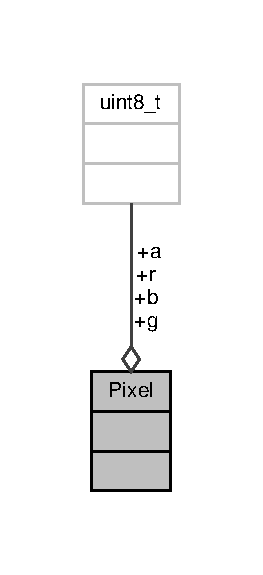
\includegraphics[width=126pt]{structPixel__coll__graph}
\end{center}
\end{figure}
\subsection*{Public Attributes}
\begin{DoxyCompactItemize}
\item 
uint8\+\_\+t \hyperlink{structPixel_a47d65d4a410f57c46746ddedd709e177}{r}
\item 
uint8\+\_\+t \hyperlink{structPixel_aeab078b7768caf273f8fe1daffa50729}{g}
\item 
uint8\+\_\+t \hyperlink{structPixel_abc9f592730eddbfcb270a1974a498d78}{b}
\item 
uint8\+\_\+t \hyperlink{structPixel_ad5c63be985fc9e1d1089907a89d7671c}{a}
\end{DoxyCompactItemize}


\subsection{Member Data Documentation}
\mbox{\Hypertarget{structPixel_ad5c63be985fc9e1d1089907a89d7671c}\label{structPixel_ad5c63be985fc9e1d1089907a89d7671c}} 
\index{Pixel@{Pixel}!a@{a}}
\index{a@{a}!Pixel@{Pixel}}
\subsubsection{\texorpdfstring{a}{a}}
{\footnotesize\ttfamily uint8\+\_\+t Pixel\+::a}

\mbox{\Hypertarget{structPixel_abc9f592730eddbfcb270a1974a498d78}\label{structPixel_abc9f592730eddbfcb270a1974a498d78}} 
\index{Pixel@{Pixel}!b@{b}}
\index{b@{b}!Pixel@{Pixel}}
\subsubsection{\texorpdfstring{b}{b}}
{\footnotesize\ttfamily uint8\+\_\+t Pixel\+::b}

\mbox{\Hypertarget{structPixel_aeab078b7768caf273f8fe1daffa50729}\label{structPixel_aeab078b7768caf273f8fe1daffa50729}} 
\index{Pixel@{Pixel}!g@{g}}
\index{g@{g}!Pixel@{Pixel}}
\subsubsection{\texorpdfstring{g}{g}}
{\footnotesize\ttfamily uint8\+\_\+t Pixel\+::g}

\mbox{\Hypertarget{structPixel_a47d65d4a410f57c46746ddedd709e177}\label{structPixel_a47d65d4a410f57c46746ddedd709e177}} 
\index{Pixel@{Pixel}!r@{r}}
\index{r@{r}!Pixel@{Pixel}}
\subsubsection{\texorpdfstring{r}{r}}
{\footnotesize\ttfamily uint8\+\_\+t Pixel\+::r}



The documentation for this struct was generated from the following file\+:\begin{DoxyCompactItemize}
\item 
inc/\hyperlink{Image_8h}{Image.\+h}\end{DoxyCompactItemize}

\hypertarget{structPlayer}{}\doxysection{Player Struct Reference}
\label{structPlayer}\index{Player@{Player}}


{\ttfamily \#include $<$Player.\+h$>$}



Collaboration diagram for Player\+:
% FIG 0
\doxysubsection*{Public Member Functions}
\begin{DoxyCompactItemize}
\item 
\mbox{\hyperlink{structPlayer_a02434d25ce99e4bedb9f30c6cd76c73c}{Player}} (\mbox{\hyperlink{structPoint}{Point}} pos=\{.x=10,.y=10\})
\item 
bool \mbox{\hyperlink{structPlayer_a743da3dcbc81ed11bfcb81943aae175b}{Moved}} () const
\item 
void \mbox{\hyperlink{structPlayer_a4b275c51f881fb61b52d1ede3d1dcba3}{Process\+Input}} (\mbox{\hyperlink{Player_8h_aa91f5cffa9b1b82e96c8824b1fe5c61f}{Movement\+Dir}} dir)
\begin{DoxyCompactList}\small\item\em Move the player from it\textquotesingle{}s current position to the direction. \end{DoxyCompactList}\item 
void \mbox{\hyperlink{structPlayer_a1a10995b61d63b46c6b562bd026382c4}{Draw}} (\mbox{\hyperlink{structImage}{Image}} \&screen)
\begin{DoxyCompactList}\small\item\em If player moved, move the player tile, save old coords. \end{DoxyCompactList}\end{DoxyCompactItemize}


\doxysubsection{Constructor \& Destructor Documentation}
\mbox{\Hypertarget{structPlayer_a02434d25ce99e4bedb9f30c6cd76c73c}\label{structPlayer_a02434d25ce99e4bedb9f30c6cd76c73c}} 
\index{Player@{Player}!Player@{Player}}
\index{Player@{Player}!Player@{Player}}
\doxysubsubsection{\texorpdfstring{Player()}{Player()}}
{\footnotesize\ttfamily Player\+::\+Player (\begin{DoxyParamCaption}\item[{\mbox{\hyperlink{structPoint}{Point}}}]{pos = {\ttfamily \{.x~=~10,~.y~=~10\}} }\end{DoxyParamCaption})\hspace{0.3cm}{\ttfamily [inline]}, {\ttfamily [explicit]}}



\doxysubsection{Member Function Documentation}
\mbox{\Hypertarget{structPlayer_a1a10995b61d63b46c6b562bd026382c4}\label{structPlayer_a1a10995b61d63b46c6b562bd026382c4}} 
\index{Player@{Player}!Draw@{Draw}}
\index{Draw@{Draw}!Player@{Player}}
\doxysubsubsection{\texorpdfstring{Draw()}{Draw()}}
{\footnotesize\ttfamily void Player\+::\+Draw (\begin{DoxyParamCaption}\item[{\mbox{\hyperlink{structImage}{Image}} \&}]{screen }\end{DoxyParamCaption})}



If player moved, move the player tile, save old coords. 


\begin{DoxyParams}{Parameters}
{\em screen} & -\/ Reference to \mbox{\hyperlink{structImage}{Image}} object on which we\textquotesingle{}re planning to draw \\
\hline
\end{DoxyParams}
Here is the call graph for this function\+:
% FIG 1
\mbox{\Hypertarget{structPlayer_a743da3dcbc81ed11bfcb81943aae175b}\label{structPlayer_a743da3dcbc81ed11bfcb81943aae175b}} 
\index{Player@{Player}!Moved@{Moved}}
\index{Moved@{Moved}!Player@{Player}}
\doxysubsubsection{\texorpdfstring{Moved()}{Moved()}}
{\footnotesize\ttfamily bool Player\+::\+Moved (\begin{DoxyParamCaption}{ }\end{DoxyParamCaption}) const}

\begin{DoxyReturn}{Returns}
true -\/ if current coordinates are equal to old 

false -\/ if current coordinates are not equal to old 
\end{DoxyReturn}
Here is the caller graph for this function\+:
% FIG 2
\mbox{\Hypertarget{structPlayer_a4b275c51f881fb61b52d1ede3d1dcba3}\label{structPlayer_a4b275c51f881fb61b52d1ede3d1dcba3}} 
\index{Player@{Player}!ProcessInput@{ProcessInput}}
\index{ProcessInput@{ProcessInput}!Player@{Player}}
\doxysubsubsection{\texorpdfstring{ProcessInput()}{ProcessInput()}}
{\footnotesize\ttfamily void Player\+::\+Process\+Input (\begin{DoxyParamCaption}\item[{\mbox{\hyperlink{Player_8h_aa91f5cffa9b1b82e96c8824b1fe5c61f}{Movement\+Dir}}}]{dir }\end{DoxyParamCaption})}



Move the player from it\textquotesingle{}s current position to the direction. 


\begin{DoxyParams}{Parameters}
{\em dir} & -\/ movement direction (of enum class Movement\+Dir) \\
\hline
\end{DoxyParams}
Here is the caller graph for this function\+:
% FIG 3


The documentation for this struct was generated from the following files\+:\begin{DoxyCompactItemize}
\item 
inc/\mbox{\hyperlink{Player_8h}{Player.\+h}}\item 
src/\mbox{\hyperlink{Player_8cpp}{Player.\+cpp}}\end{DoxyCompactItemize}

\hypertarget{structPoint}{}\doxysection{Point Struct Reference}
\label{structPoint}\index{Point@{Point}}


{\ttfamily \#include $<$Player.\+h$>$}



Collaboration diagram for Point\+:
% FIG 0
\doxysubsection*{Public Attributes}
\begin{DoxyCompactItemize}
\item 
int \mbox{\hyperlink{structPoint_a8c779e11e694b20e0946105a9f5de842}{x}}
\item 
int \mbox{\hyperlink{structPoint_a2e1b5fb2b2a83571f5c0bc0f66a73cf7}{y}}
\end{DoxyCompactItemize}


\doxysubsection{Member Data Documentation}
\mbox{\Hypertarget{structPoint_a8c779e11e694b20e0946105a9f5de842}\label{structPoint_a8c779e11e694b20e0946105a9f5de842}} 
\index{Point@{Point}!x@{x}}
\index{x@{x}!Point@{Point}}
\doxysubsubsection{\texorpdfstring{x}{x}}
{\footnotesize\ttfamily int Point\+::x}

\mbox{\Hypertarget{structPoint_a2e1b5fb2b2a83571f5c0bc0f66a73cf7}\label{structPoint_a2e1b5fb2b2a83571f5c0bc0f66a73cf7}} 
\index{Point@{Point}!y@{y}}
\index{y@{y}!Point@{Point}}
\doxysubsubsection{\texorpdfstring{y}{y}}
{\footnotesize\ttfamily int Point\+::y}



The documentation for this struct was generated from the following file\+:\begin{DoxyCompactItemize}
\item 
inc/gameplay/\mbox{\hyperlink{Player_8h}{Player.\+h}}\end{DoxyCompactItemize}

\hypertarget{structstbi__io__callbacks}{}\doxysection{stbi\+\_\+io\+\_\+callbacks Struct Reference}
\label{structstbi__io__callbacks}\index{stbi\_io\_callbacks@{stbi\_io\_callbacks}}


{\ttfamily \#include $<$stb\+\_\+image.\+h$>$}



Collaboration diagram for stbi\+\_\+io\+\_\+callbacks\+:
% FIG 0
\doxysubsection*{Public Attributes}
\begin{DoxyCompactItemize}
\item 
int($\ast$ \mbox{\hyperlink{structstbi__io__callbacks_a623e46b3a2a019611601409926283a88}{read}} )(void $\ast$user, char $\ast$data, int size)
\item 
void($\ast$ \mbox{\hyperlink{structstbi__io__callbacks_a257aac5480a90a6c4b8fbe86c1b01068}{skip}} )(void $\ast$user, int n)
\item 
int($\ast$ \mbox{\hyperlink{structstbi__io__callbacks_a319639db2f76e715eed7a7a974136832}{eof}} )(void $\ast$user)
\end{DoxyCompactItemize}


\doxysubsection{Member Data Documentation}
\mbox{\Hypertarget{structstbi__io__callbacks_a319639db2f76e715eed7a7a974136832}\label{structstbi__io__callbacks_a319639db2f76e715eed7a7a974136832}} 
\index{stbi\_io\_callbacks@{stbi\_io\_callbacks}!eof@{eof}}
\index{eof@{eof}!stbi\_io\_callbacks@{stbi\_io\_callbacks}}
\doxysubsubsection{\texorpdfstring{eof}{eof}}
{\footnotesize\ttfamily int($\ast$ stbi\+\_\+io\+\_\+callbacks\+::eof) (void $\ast$user)}

\mbox{\Hypertarget{structstbi__io__callbacks_a623e46b3a2a019611601409926283a88}\label{structstbi__io__callbacks_a623e46b3a2a019611601409926283a88}} 
\index{stbi\_io\_callbacks@{stbi\_io\_callbacks}!read@{read}}
\index{read@{read}!stbi\_io\_callbacks@{stbi\_io\_callbacks}}
\doxysubsubsection{\texorpdfstring{read}{read}}
{\footnotesize\ttfamily int($\ast$ stbi\+\_\+io\+\_\+callbacks\+::read) (void $\ast$user, char $\ast$data, int size)}

\mbox{\Hypertarget{structstbi__io__callbacks_a257aac5480a90a6c4b8fbe86c1b01068}\label{structstbi__io__callbacks_a257aac5480a90a6c4b8fbe86c1b01068}} 
\index{stbi\_io\_callbacks@{stbi\_io\_callbacks}!skip@{skip}}
\index{skip@{skip}!stbi\_io\_callbacks@{stbi\_io\_callbacks}}
\doxysubsubsection{\texorpdfstring{skip}{skip}}
{\footnotesize\ttfamily void($\ast$ stbi\+\_\+io\+\_\+callbacks\+::skip) (void $\ast$user, int n)}



The documentation for this struct was generated from the following file\+:\begin{DoxyCompactItemize}
\item 
inc/graphics/\mbox{\hyperlink{stb__image_8h}{stb\+\_\+image.\+h}}\end{DoxyCompactItemize}

\chapter{File Documentation}
\hypertarget{common_8h}{}\section{inc/common.h File Reference}
\label{common_8h}\index{inc/common.\+h@{inc/common.\+h}}


File Which co.  


{\ttfamily \#include $<$iostream$>$}\newline
{\ttfamily \#include $<$fstream$>$}\newline
{\ttfamily \#include $<$string$>$}\newline
{\ttfamily \#include $<$glad/glad.\+h$>$}\newline
Include dependency graph for common.\+h\+:
\nopagebreak
\begin{figure}[H]
\begin{center}
\leavevmode
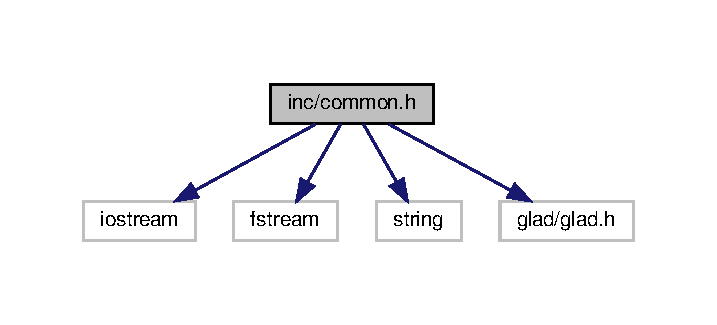
\includegraphics[width=344pt]{common_8h__incl}
\end{center}
\end{figure}
This graph shows which files directly or indirectly include this file\+:
\nopagebreak
\begin{figure}[H]
\begin{center}
\leavevmode
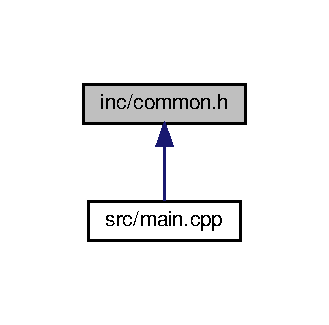
\includegraphics[width=158pt]{common_8h__dep__incl}
\end{center}
\end{figure}
\subsection*{Macros}
\begin{DoxyCompactItemize}
\item 
\#define \hyperlink{common_8h_a0c19729acaa7baef460908e525be0e7f}{G\+L\+\_\+\+C\+H\+E\+C\+K\+\_\+\+E\+R\+R\+O\+RS}~Throw\+Exception\+On\+G\+L\+Error(\+\_\+\+\_\+\+L\+I\+N\+E\+\_\+\+\_\+,\+\_\+\+\_\+\+F\+I\+L\+E\+\_\+\+\_\+);
\end{DoxyCompactItemize}


\subsection{Detailed Description}
File Which co. 

Details. 

\subsection{Macro Definition Documentation}
\mbox{\Hypertarget{common_8h_a0c19729acaa7baef460908e525be0e7f}\label{common_8h_a0c19729acaa7baef460908e525be0e7f}} 
\index{common.\+h@{common.\+h}!G\+L\+\_\+\+C\+H\+E\+C\+K\+\_\+\+E\+R\+R\+O\+RS@{G\+L\+\_\+\+C\+H\+E\+C\+K\+\_\+\+E\+R\+R\+O\+RS}}
\index{G\+L\+\_\+\+C\+H\+E\+C\+K\+\_\+\+E\+R\+R\+O\+RS@{G\+L\+\_\+\+C\+H\+E\+C\+K\+\_\+\+E\+R\+R\+O\+RS}!common.\+h@{common.\+h}}
\subsubsection{\texorpdfstring{G\+L\+\_\+\+C\+H\+E\+C\+K\+\_\+\+E\+R\+R\+O\+RS}{GL\_CHECK\_ERRORS}}
{\footnotesize\ttfamily \#define G\+L\+\_\+\+C\+H\+E\+C\+K\+\_\+\+E\+R\+R\+O\+RS~Throw\+Exception\+On\+G\+L\+Error(\+\_\+\+\_\+\+L\+I\+N\+E\+\_\+\+\_\+,\+\_\+\+\_\+\+F\+I\+L\+E\+\_\+\+\_\+);}


\hypertarget{Image_8h}{}\doxysection{inc/\+Image.h File Reference}
\label{Image_8h}\index{inc/Image.h@{inc/Image.h}}


\mbox{\hyperlink{structImage}{Image}} and \mbox{\hyperlink{structPixel}{Pixel}} representation.  


{\ttfamily \#include $<$string$>$}\newline
Include dependency graph for Image.\+h\+:
\nopagebreak
\begin{figure}[H]
\begin{center}
\leavevmode
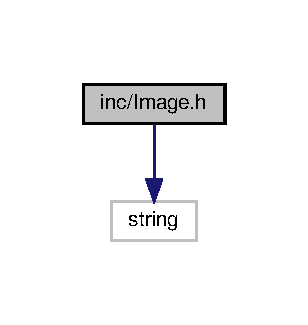
\includegraphics[width=148pt]{Image_8h__incl}
\end{center}
\end{figure}
This graph shows which files directly or indirectly include this file\+:
\nopagebreak
\begin{figure}[H]
\begin{center}
\leavevmode
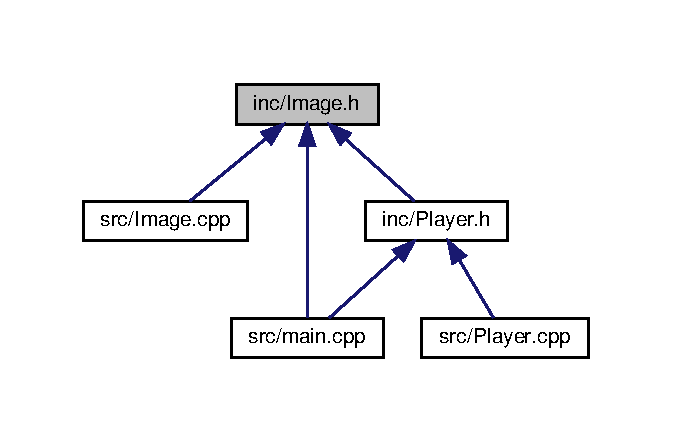
\includegraphics[width=323pt]{Image_8h__dep__incl}
\end{center}
\end{figure}
\doxysubsection*{Classes}
\begin{DoxyCompactItemize}
\item 
struct \mbox{\hyperlink{structPixel}{Pixel}}
\begin{DoxyCompactList}\small\item\em \mbox{\hyperlink{structPixel}{Pixel}} in R\+G\+BA representation. \end{DoxyCompactList}\item 
struct \mbox{\hyperlink{structImage}{Image}}
\begin{DoxyCompactList}\small\item\em Class representation of \mbox{\hyperlink{structImage}{Image}} abstraction. \end{DoxyCompactList}\end{DoxyCompactItemize}
\doxysubsection*{Variables}
\begin{DoxyCompactItemize}
\item 
constexpr int \mbox{\hyperlink{Image_8h_a23cad1852a877fb7d9bb6c37452073c7}{tile\+Size}} = 16
\item 
constexpr \mbox{\hyperlink{structPixel}{Pixel}} \mbox{\hyperlink{Image_8h_a7b2ce04fb84806f4dd901b6c8b426a28}{background\+Color}} \{0, 0, 0, 0\}
\end{DoxyCompactItemize}


\doxysubsection{Detailed Description}
\mbox{\hyperlink{structImage}{Image}} and \mbox{\hyperlink{structPixel}{Pixel}} representation. 



\doxysubsection{Variable Documentation}
\mbox{\Hypertarget{Image_8h_a7b2ce04fb84806f4dd901b6c8b426a28}\label{Image_8h_a7b2ce04fb84806f4dd901b6c8b426a28}} 
\index{Image.h@{Image.h}!backgroundColor@{backgroundColor}}
\index{backgroundColor@{backgroundColor}!Image.h@{Image.h}}
\doxysubsubsection{\texorpdfstring{backgroundColor}{backgroundColor}}
{\footnotesize\ttfamily constexpr \mbox{\hyperlink{structPixel}{Pixel}} background\+Color \{0, 0, 0, 0\}\hspace{0.3cm}{\ttfamily [constexpr]}}

\mbox{\Hypertarget{Image_8h_a23cad1852a877fb7d9bb6c37452073c7}\label{Image_8h_a23cad1852a877fb7d9bb6c37452073c7}} 
\index{Image.h@{Image.h}!tileSize@{tileSize}}
\index{tileSize@{tileSize}!Image.h@{Image.h}}
\doxysubsubsection{\texorpdfstring{tileSize}{tileSize}}
{\footnotesize\ttfamily constexpr int tile\+Size = 16\hspace{0.3cm}{\ttfamily [constexpr]}}


\hypertarget{Player_8h}{}\doxysection{inc/\+Player.h File Reference}
\label{Player_8h}\index{inc/Player.h@{inc/Player.h}}


\mbox{\hyperlink{structPoint}{Point}}, Movement\+Direction and \mbox{\hyperlink{structPlayer}{Player}} classes.  


{\ttfamily \#include \char`\"{}Image.\+h\char`\"{}}\newline
Include dependency graph for Player.\+h\+:
% FIG 0
This graph shows which files directly or indirectly include this file\+:
% FIG 1
\doxysubsection*{Classes}
\begin{DoxyCompactItemize}
\item 
struct \mbox{\hyperlink{structPoint}{Point}}
\item 
struct \mbox{\hyperlink{structPlayer}{Player}}
\end{DoxyCompactItemize}
\doxysubsection*{Enumerations}
\begin{DoxyCompactItemize}
\item 
enum \mbox{\hyperlink{Player_8h_aa91f5cffa9b1b82e96c8824b1fe5c61f}{Movement\+Dir}} \{ \mbox{\hyperlink{Player_8h_aa91f5cffa9b1b82e96c8824b1fe5c61fafbaedde498cdead4f2780217646e9ba1}{Movement\+Dir\+::\+UP}}, 
\mbox{\hyperlink{Player_8h_aa91f5cffa9b1b82e96c8824b1fe5c61fac4e0e4e3118472beeb2ae75827450f1f}{Movement\+Dir\+::\+D\+O\+WN}}, 
\mbox{\hyperlink{Player_8h_aa91f5cffa9b1b82e96c8824b1fe5c61fa684d325a7303f52e64011467ff5c5758}{Movement\+Dir\+::\+L\+E\+FT}}, 
\mbox{\hyperlink{Player_8h_aa91f5cffa9b1b82e96c8824b1fe5c61fa21507b40c80068eda19865706fdc2403}{Movement\+Dir\+::\+R\+I\+G\+HT}}
 \}
\end{DoxyCompactItemize}


\doxysubsection{Detailed Description}
\mbox{\hyperlink{structPoint}{Point}}, Movement\+Direction and \mbox{\hyperlink{structPlayer}{Player}} classes. 



\doxysubsection{Enumeration Type Documentation}
\mbox{\Hypertarget{Player_8h_aa91f5cffa9b1b82e96c8824b1fe5c61f}\label{Player_8h_aa91f5cffa9b1b82e96c8824b1fe5c61f}} 
\index{Player.h@{Player.h}!MovementDir@{MovementDir}}
\index{MovementDir@{MovementDir}!Player.h@{Player.h}}
\doxysubsubsection{\texorpdfstring{MovementDir}{MovementDir}}
{\footnotesize\ttfamily enum \mbox{\hyperlink{Player_8h_aa91f5cffa9b1b82e96c8824b1fe5c61f}{Movement\+Dir}}\hspace{0.3cm}{\ttfamily [strong]}}

\begin{DoxyEnumFields}{Enumerator}
\raisebox{\heightof{T}}[0pt][0pt]{\index{UP@{UP}!Player.h@{Player.h}}\index{Player.h@{Player.h}!UP@{UP}}}\mbox{\Hypertarget{Player_8h_aa91f5cffa9b1b82e96c8824b1fe5c61fafbaedde498cdead4f2780217646e9ba1}\label{Player_8h_aa91f5cffa9b1b82e96c8824b1fe5c61fafbaedde498cdead4f2780217646e9ba1}} 
UP&\\
\hline

\raisebox{\heightof{T}}[0pt][0pt]{\index{DOWN@{DOWN}!Player.h@{Player.h}}\index{Player.h@{Player.h}!DOWN@{DOWN}}}\mbox{\Hypertarget{Player_8h_aa91f5cffa9b1b82e96c8824b1fe5c61fac4e0e4e3118472beeb2ae75827450f1f}\label{Player_8h_aa91f5cffa9b1b82e96c8824b1fe5c61fac4e0e4e3118472beeb2ae75827450f1f}} 
D\+O\+WN&\\
\hline

\raisebox{\heightof{T}}[0pt][0pt]{\index{LEFT@{LEFT}!Player.h@{Player.h}}\index{Player.h@{Player.h}!LEFT@{LEFT}}}\mbox{\Hypertarget{Player_8h_aa91f5cffa9b1b82e96c8824b1fe5c61fa684d325a7303f52e64011467ff5c5758}\label{Player_8h_aa91f5cffa9b1b82e96c8824b1fe5c61fa684d325a7303f52e64011467ff5c5758}} 
L\+E\+FT&\\
\hline

\raisebox{\heightof{T}}[0pt][0pt]{\index{RIGHT@{RIGHT}!Player.h@{Player.h}}\index{Player.h@{Player.h}!RIGHT@{RIGHT}}}\mbox{\Hypertarget{Player_8h_aa91f5cffa9b1b82e96c8824b1fe5c61fa21507b40c80068eda19865706fdc2403}\label{Player_8h_aa91f5cffa9b1b82e96c8824b1fe5c61fa21507b40c80068eda19865706fdc2403}} 
R\+I\+G\+HT&\\
\hline

\end{DoxyEnumFields}

\hypertarget{stb__image_8h}{}\section{inc/stb\+\_\+image.h File Reference}
\label{stb__image_8h}\index{inc/stb\+\_\+image.\+h@{inc/stb\+\_\+image.\+h}}
{\ttfamily \#include $<$stdio.\+h$>$}\newline
{\ttfamily \#include $<$stdlib.\+h$>$}\newline
Include dependency graph for stb\+\_\+image.\+h\+:
\nopagebreak
\begin{figure}[H]
\begin{center}
\leavevmode
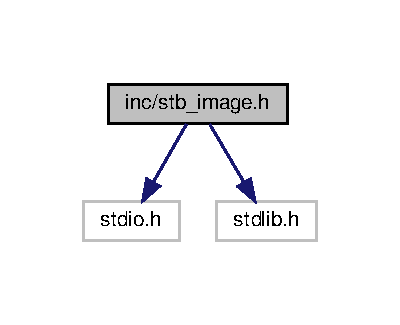
\includegraphics[width=192pt]{stb__image_8h__incl}
\end{center}
\end{figure}
This graph shows which files directly or indirectly include this file\+:
\nopagebreak
\begin{figure}[H]
\begin{center}
\leavevmode
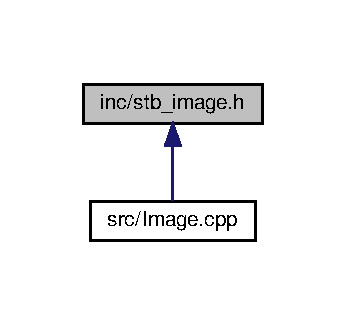
\includegraphics[width=166pt]{stb__image_8h__dep__incl}
\end{center}
\end{figure}
\subsection*{Classes}
\begin{DoxyCompactItemize}
\item 
struct \hyperlink{structstbi__io__callbacks}{stbi\+\_\+io\+\_\+callbacks}
\end{DoxyCompactItemize}
\subsection*{Macros}
\begin{DoxyCompactItemize}
\item 
\#define \hyperlink{stb__image_8h_aed6cd14a3bf678808c4c179e808866aa}{S\+T\+B\+I\+\_\+\+V\+E\+R\+S\+I\+ON}~1
\item 
\#define \hyperlink{stb__image_8h_a2d9ec9850cd12aefe7641b456266a4c2}{S\+T\+B\+I\+D\+EF}~extern
\end{DoxyCompactItemize}
\subsection*{Typedefs}
\begin{DoxyCompactItemize}
\item 
typedef unsigned char \hyperlink{stb__image_8h_a28eb51a1512ce382ee50f20e1d04d50d}{stbi\+\_\+uc}
\item 
typedef unsigned short \hyperlink{stb__image_8h_a648037d4c55689328ba08c8f5d293df2}{stbi\+\_\+us}
\end{DoxyCompactItemize}
\subsection*{Enumerations}
\begin{DoxyCompactItemize}
\item 
enum \{ \newline
\hyperlink{stb__image_8h_a06fc87d81c62e9abb8790b6e5713c55ba0177ac2c5002f4f251bb766d41752029}{S\+T\+B\+I\+\_\+default} = 0, 
\hyperlink{stb__image_8h_a06fc87d81c62e9abb8790b6e5713c55bad1eb95ca1fa7706bf732bf35a0ed40aa}{S\+T\+B\+I\+\_\+grey} = 1, 
\hyperlink{stb__image_8h_a06fc87d81c62e9abb8790b6e5713c55baf5829d16d4cca6077465c5abd346e2f8}{S\+T\+B\+I\+\_\+grey\+\_\+alpha} = 2, 
\hyperlink{stb__image_8h_a06fc87d81c62e9abb8790b6e5713c55baa59123e5d0af25f9b1539f5cf1facddf}{S\+T\+B\+I\+\_\+rgb} = 3, 
\newline
\hyperlink{stb__image_8h_a06fc87d81c62e9abb8790b6e5713c55baa7b1af0c9f0310c3ada2aa29a32de293}{S\+T\+B\+I\+\_\+rgb\+\_\+alpha} = 4
 \}
\end{DoxyCompactItemize}
\subsection*{Functions}
\begin{DoxyCompactItemize}
\item 
\hyperlink{stb__image_8h_a2d9ec9850cd12aefe7641b456266a4c2}{S\+T\+B\+I\+D\+EF} \hyperlink{stb__image_8h_a28eb51a1512ce382ee50f20e1d04d50d}{stbi\+\_\+uc} $\ast$ \hyperlink{stb__image_8h_acae25d31bfae29d75482f07fecf2935f}{stbi\+\_\+load\+\_\+from\+\_\+memory} (\hyperlink{stb__image_8h_a28eb51a1512ce382ee50f20e1d04d50d}{stbi\+\_\+uc} const $\ast$buffer, int len, int $\ast$x, int $\ast$y, int $\ast$channels\+\_\+in\+\_\+file, int desired\+\_\+channels)
\item 
\hyperlink{stb__image_8h_a2d9ec9850cd12aefe7641b456266a4c2}{S\+T\+B\+I\+D\+EF} \hyperlink{stb__image_8h_a28eb51a1512ce382ee50f20e1d04d50d}{stbi\+\_\+uc} $\ast$ \hyperlink{stb__image_8h_a95ebc5c42c1a753200be8d465e933af7}{stbi\+\_\+load\+\_\+from\+\_\+callbacks} (\hyperlink{structstbi__io__callbacks}{stbi\+\_\+io\+\_\+callbacks} const $\ast$clbk, void $\ast$user, int $\ast$x, int $\ast$y, int $\ast$channels\+\_\+in\+\_\+file, int desired\+\_\+channels)
\item 
\hyperlink{stb__image_8h_a2d9ec9850cd12aefe7641b456266a4c2}{S\+T\+B\+I\+D\+EF} \hyperlink{stb__image_8h_a28eb51a1512ce382ee50f20e1d04d50d}{stbi\+\_\+uc} $\ast$ \hyperlink{stb__image_8h_aefdc7387857a14894bbf321e9ea4f048}{stbi\+\_\+load} (char const $\ast$filename, int $\ast$x, int $\ast$y, int $\ast$channels\+\_\+in\+\_\+file, int desired\+\_\+channels)
\item 
\hyperlink{stb__image_8h_a2d9ec9850cd12aefe7641b456266a4c2}{S\+T\+B\+I\+D\+EF} \hyperlink{stb__image_8h_a28eb51a1512ce382ee50f20e1d04d50d}{stbi\+\_\+uc} $\ast$ \hyperlink{stb__image_8h_aa9994764695597161e8f3776e97caa99}{stbi\+\_\+load\+\_\+from\+\_\+file} (F\+I\+LE $\ast$f, int $\ast$x, int $\ast$y, int $\ast$channels\+\_\+in\+\_\+file, int desired\+\_\+channels)
\item 
\hyperlink{stb__image_8h_a2d9ec9850cd12aefe7641b456266a4c2}{S\+T\+B\+I\+D\+EF} \hyperlink{stb__image_8h_a28eb51a1512ce382ee50f20e1d04d50d}{stbi\+\_\+uc} $\ast$ \hyperlink{stb__image_8h_ab81ccbc3526368d651117ef48df82b01}{stbi\+\_\+load\+\_\+gif\+\_\+from\+\_\+memory} (\hyperlink{stb__image_8h_a28eb51a1512ce382ee50f20e1d04d50d}{stbi\+\_\+uc} const $\ast$buffer, int len, int $\ast$$\ast$delays, int $\ast$x, int $\ast$y, int $\ast$z, int $\ast$comp, int req\+\_\+comp)
\item 
\hyperlink{stb__image_8h_a2d9ec9850cd12aefe7641b456266a4c2}{S\+T\+B\+I\+D\+EF} \hyperlink{stb__image_8h_a648037d4c55689328ba08c8f5d293df2}{stbi\+\_\+us} $\ast$ \hyperlink{stb__image_8h_ad30fd870ed2138ce8f38c9dd29b2f76a}{stbi\+\_\+load\+\_\+16\+\_\+from\+\_\+memory} (\hyperlink{stb__image_8h_a28eb51a1512ce382ee50f20e1d04d50d}{stbi\+\_\+uc} const $\ast$buffer, int len, int $\ast$x, int $\ast$y, int $\ast$channels\+\_\+in\+\_\+file, int desired\+\_\+channels)
\item 
\hyperlink{stb__image_8h_a2d9ec9850cd12aefe7641b456266a4c2}{S\+T\+B\+I\+D\+EF} \hyperlink{stb__image_8h_a648037d4c55689328ba08c8f5d293df2}{stbi\+\_\+us} $\ast$ \hyperlink{stb__image_8h_a82bcc0957b6a4ebfdfa3d7f04fbaed18}{stbi\+\_\+load\+\_\+16\+\_\+from\+\_\+callbacks} (\hyperlink{structstbi__io__callbacks}{stbi\+\_\+io\+\_\+callbacks} const $\ast$clbk, void $\ast$user, int $\ast$x, int $\ast$y, int $\ast$channels\+\_\+in\+\_\+file, int desired\+\_\+channels)
\item 
\hyperlink{stb__image_8h_a2d9ec9850cd12aefe7641b456266a4c2}{S\+T\+B\+I\+D\+EF} \hyperlink{stb__image_8h_a648037d4c55689328ba08c8f5d293df2}{stbi\+\_\+us} $\ast$ \hyperlink{stb__image_8h_a8a58b6bcd805afa1bdb14f988dd37fee}{stbi\+\_\+load\+\_\+16} (char const $\ast$filename, int $\ast$x, int $\ast$y, int $\ast$channels\+\_\+in\+\_\+file, int desired\+\_\+channels)
\item 
\hyperlink{stb__image_8h_a2d9ec9850cd12aefe7641b456266a4c2}{S\+T\+B\+I\+D\+EF} \hyperlink{stb__image_8h_a648037d4c55689328ba08c8f5d293df2}{stbi\+\_\+us} $\ast$ \hyperlink{stb__image_8h_a9ca2591f0987284129e82bf9dbcf7c6c}{stbi\+\_\+load\+\_\+from\+\_\+file\+\_\+16} (F\+I\+LE $\ast$f, int $\ast$x, int $\ast$y, int $\ast$channels\+\_\+in\+\_\+file, int desired\+\_\+channels)
\item 
\hyperlink{stb__image_8h_a2d9ec9850cd12aefe7641b456266a4c2}{S\+T\+B\+I\+D\+EF} float $\ast$ \hyperlink{stb__image_8h_a5d47fb76ce1e34eb0729ad932c9c48e2}{stbi\+\_\+loadf\+\_\+from\+\_\+memory} (\hyperlink{stb__image_8h_a28eb51a1512ce382ee50f20e1d04d50d}{stbi\+\_\+uc} const $\ast$buffer, int len, int $\ast$x, int $\ast$y, int $\ast$channels\+\_\+in\+\_\+file, int desired\+\_\+channels)
\item 
\hyperlink{stb__image_8h_a2d9ec9850cd12aefe7641b456266a4c2}{S\+T\+B\+I\+D\+EF} float $\ast$ \hyperlink{stb__image_8h_a6e7fd261af79ecef2208df3a6cc806bb}{stbi\+\_\+loadf\+\_\+from\+\_\+callbacks} (\hyperlink{structstbi__io__callbacks}{stbi\+\_\+io\+\_\+callbacks} const $\ast$clbk, void $\ast$user, int $\ast$x, int $\ast$y, int $\ast$channels\+\_\+in\+\_\+file, int desired\+\_\+channels)
\item 
\hyperlink{stb__image_8h_a2d9ec9850cd12aefe7641b456266a4c2}{S\+T\+B\+I\+D\+EF} float $\ast$ \hyperlink{stb__image_8h_af4f17acd30945a75901fdc022f90575f}{stbi\+\_\+loadf} (char const $\ast$filename, int $\ast$x, int $\ast$y, int $\ast$channels\+\_\+in\+\_\+file, int desired\+\_\+channels)
\item 
\hyperlink{stb__image_8h_a2d9ec9850cd12aefe7641b456266a4c2}{S\+T\+B\+I\+D\+EF} float $\ast$ \hyperlink{stb__image_8h_ace82446ecd7b5c760cde062179660f46}{stbi\+\_\+loadf\+\_\+from\+\_\+file} (F\+I\+LE $\ast$f, int $\ast$x, int $\ast$y, int $\ast$channels\+\_\+in\+\_\+file, int desired\+\_\+channels)
\item 
\hyperlink{stb__image_8h_a2d9ec9850cd12aefe7641b456266a4c2}{S\+T\+B\+I\+D\+EF} void \hyperlink{stb__image_8h_ab18889e43518d6b4421b705782bb1b5e}{stbi\+\_\+hdr\+\_\+to\+\_\+ldr\+\_\+gamma} (float gamma)
\item 
\hyperlink{stb__image_8h_a2d9ec9850cd12aefe7641b456266a4c2}{S\+T\+B\+I\+D\+EF} void \hyperlink{stb__image_8h_ae21cc1184eeb5cc814699f1ed62c5258}{stbi\+\_\+hdr\+\_\+to\+\_\+ldr\+\_\+scale} (float scale)
\item 
\hyperlink{stb__image_8h_a2d9ec9850cd12aefe7641b456266a4c2}{S\+T\+B\+I\+D\+EF} void \hyperlink{stb__image_8h_a1feccdcf726dcc6b5502e3efa85b7dbb}{stbi\+\_\+ldr\+\_\+to\+\_\+hdr\+\_\+gamma} (float gamma)
\item 
\hyperlink{stb__image_8h_a2d9ec9850cd12aefe7641b456266a4c2}{S\+T\+B\+I\+D\+EF} void \hyperlink{stb__image_8h_af946583656a362a316b40c0421c20561}{stbi\+\_\+ldr\+\_\+to\+\_\+hdr\+\_\+scale} (float scale)
\item 
\hyperlink{stb__image_8h_a2d9ec9850cd12aefe7641b456266a4c2}{S\+T\+B\+I\+D\+EF} int \hyperlink{stb__image_8h_af0e94f316fe1848f632517ca3c11d077}{stbi\+\_\+is\+\_\+hdr\+\_\+from\+\_\+callbacks} (\hyperlink{structstbi__io__callbacks}{stbi\+\_\+io\+\_\+callbacks} const $\ast$clbk, void $\ast$user)
\item 
\hyperlink{stb__image_8h_a2d9ec9850cd12aefe7641b456266a4c2}{S\+T\+B\+I\+D\+EF} int \hyperlink{stb__image_8h_a5cbc6f5cbb3b2d0d87ee959fcee9d23e}{stbi\+\_\+is\+\_\+hdr\+\_\+from\+\_\+memory} (\hyperlink{stb__image_8h_a28eb51a1512ce382ee50f20e1d04d50d}{stbi\+\_\+uc} const $\ast$buffer, int len)
\item 
\hyperlink{stb__image_8h_a2d9ec9850cd12aefe7641b456266a4c2}{S\+T\+B\+I\+D\+EF} int \hyperlink{stb__image_8h_ae70f9a302f7e87fd971075e7f758d55c}{stbi\+\_\+is\+\_\+hdr} (char const $\ast$filename)
\item 
\hyperlink{stb__image_8h_a2d9ec9850cd12aefe7641b456266a4c2}{S\+T\+B\+I\+D\+EF} int \hyperlink{stb__image_8h_aaf10d41631e1e9214fde1688bdbd8524}{stbi\+\_\+is\+\_\+hdr\+\_\+from\+\_\+file} (F\+I\+LE $\ast$f)
\item 
\hyperlink{stb__image_8h_a2d9ec9850cd12aefe7641b456266a4c2}{S\+T\+B\+I\+D\+EF} const char $\ast$ \hyperlink{stb__image_8h_aa874b3ba909f3281d499894909678336}{stbi\+\_\+failure\+\_\+reason} (void)
\item 
\hyperlink{stb__image_8h_a2d9ec9850cd12aefe7641b456266a4c2}{S\+T\+B\+I\+D\+EF} void \hyperlink{stb__image_8h_ad3e11bb44412a7ba348acfbad09caacb}{stbi\+\_\+image\+\_\+free} (void $\ast$retval\+\_\+from\+\_\+stbi\+\_\+load)
\item 
\hyperlink{stb__image_8h_a2d9ec9850cd12aefe7641b456266a4c2}{S\+T\+B\+I\+D\+EF} int \hyperlink{stb__image_8h_acfef077febce3bc3f1f339de478f3315}{stbi\+\_\+info\+\_\+from\+\_\+memory} (\hyperlink{stb__image_8h_a28eb51a1512ce382ee50f20e1d04d50d}{stbi\+\_\+uc} const $\ast$buffer, int len, int $\ast$x, int $\ast$y, int $\ast$comp)
\item 
\hyperlink{stb__image_8h_a2d9ec9850cd12aefe7641b456266a4c2}{S\+T\+B\+I\+D\+EF} int \hyperlink{stb__image_8h_a86291c64cb663f41a34647d5e1abf363}{stbi\+\_\+info\+\_\+from\+\_\+callbacks} (\hyperlink{structstbi__io__callbacks}{stbi\+\_\+io\+\_\+callbacks} const $\ast$clbk, void $\ast$user, int $\ast$x, int $\ast$y, int $\ast$comp)
\item 
\hyperlink{stb__image_8h_a2d9ec9850cd12aefe7641b456266a4c2}{S\+T\+B\+I\+D\+EF} int \hyperlink{stb__image_8h_a548d486e07e0eb95671cb200d3a9530f}{stbi\+\_\+is\+\_\+16\+\_\+bit\+\_\+from\+\_\+memory} (\hyperlink{stb__image_8h_a28eb51a1512ce382ee50f20e1d04d50d}{stbi\+\_\+uc} const $\ast$buffer, int len)
\item 
\hyperlink{stb__image_8h_a2d9ec9850cd12aefe7641b456266a4c2}{S\+T\+B\+I\+D\+EF} int \hyperlink{stb__image_8h_a990e0e38ab6e600bd9cbf5d30abd2f8f}{stbi\+\_\+is\+\_\+16\+\_\+bit\+\_\+from\+\_\+callbacks} (\hyperlink{structstbi__io__callbacks}{stbi\+\_\+io\+\_\+callbacks} const $\ast$clbk, void $\ast$user)
\item 
\hyperlink{stb__image_8h_a2d9ec9850cd12aefe7641b456266a4c2}{S\+T\+B\+I\+D\+EF} int \hyperlink{stb__image_8h_aede708cca1304520b2afcf4d5eb61d70}{stbi\+\_\+info} (char const $\ast$filename, int $\ast$x, int $\ast$y, int $\ast$comp)
\item 
\hyperlink{stb__image_8h_a2d9ec9850cd12aefe7641b456266a4c2}{S\+T\+B\+I\+D\+EF} int \hyperlink{stb__image_8h_a28abedef4a0a93909332080df6be0021}{stbi\+\_\+info\+\_\+from\+\_\+file} (F\+I\+LE $\ast$f, int $\ast$x, int $\ast$y, int $\ast$comp)
\item 
\hyperlink{stb__image_8h_a2d9ec9850cd12aefe7641b456266a4c2}{S\+T\+B\+I\+D\+EF} int \hyperlink{stb__image_8h_a7d9af55a35382c011cc186f7b62c00af}{stbi\+\_\+is\+\_\+16\+\_\+bit} (char const $\ast$filename)
\item 
\hyperlink{stb__image_8h_a2d9ec9850cd12aefe7641b456266a4c2}{S\+T\+B\+I\+D\+EF} int \hyperlink{stb__image_8h_a42fa266b80bfde22a0781ba2112d1c62}{stbi\+\_\+is\+\_\+16\+\_\+bit\+\_\+from\+\_\+file} (F\+I\+LE $\ast$f)
\item 
\hyperlink{stb__image_8h_a2d9ec9850cd12aefe7641b456266a4c2}{S\+T\+B\+I\+D\+EF} void \hyperlink{stb__image_8h_a3f02e0053e1c8d08a3ed436e6a82c7c9}{stbi\+\_\+set\+\_\+unpremultiply\+\_\+on\+\_\+load} (int flag\+\_\+true\+\_\+if\+\_\+should\+\_\+unpremultiply)
\item 
\hyperlink{stb__image_8h_a2d9ec9850cd12aefe7641b456266a4c2}{S\+T\+B\+I\+D\+EF} void \hyperlink{stb__image_8h_a23525ef2b882f3de426b47ecf8d9151b}{stbi\+\_\+convert\+\_\+iphone\+\_\+png\+\_\+to\+\_\+rgb} (int flag\+\_\+true\+\_\+if\+\_\+should\+\_\+convert)
\item 
\hyperlink{stb__image_8h_a2d9ec9850cd12aefe7641b456266a4c2}{S\+T\+B\+I\+D\+EF} void \hyperlink{stb__image_8h_ab89c177fc52f1bb2dc1c05e48129a0a4}{stbi\+\_\+set\+\_\+flip\+\_\+vertically\+\_\+on\+\_\+load} (int flag\+\_\+true\+\_\+if\+\_\+should\+\_\+flip)
\item 
\hyperlink{stb__image_8h_a2d9ec9850cd12aefe7641b456266a4c2}{S\+T\+B\+I\+D\+EF} void \hyperlink{stb__image_8h_ad683202a3f6ec89729b5ad9220ae98ee}{stbi\+\_\+set\+\_\+flip\+\_\+vertically\+\_\+on\+\_\+load\+\_\+thread} (int flag\+\_\+true\+\_\+if\+\_\+should\+\_\+flip)
\item 
\hyperlink{stb__image_8h_a2d9ec9850cd12aefe7641b456266a4c2}{S\+T\+B\+I\+D\+EF} char $\ast$ \hyperlink{stb__image_8h_aaaa17a529bec51403cc23dc2e7c36d79}{stbi\+\_\+zlib\+\_\+decode\+\_\+malloc\+\_\+guesssize} (const char $\ast$buffer, int len, int initial\+\_\+size, int $\ast$outlen)
\item 
\hyperlink{stb__image_8h_a2d9ec9850cd12aefe7641b456266a4c2}{S\+T\+B\+I\+D\+EF} char $\ast$ \hyperlink{stb__image_8h_a038b0e741859a482b8b9d60167e54d27}{stbi\+\_\+zlib\+\_\+decode\+\_\+malloc\+\_\+guesssize\+\_\+headerflag} (const char $\ast$buffer, int len, int initial\+\_\+size, int $\ast$outlen, int parse\+\_\+header)
\item 
\hyperlink{stb__image_8h_a2d9ec9850cd12aefe7641b456266a4c2}{S\+T\+B\+I\+D\+EF} char $\ast$ \hyperlink{stb__image_8h_a4919b67b12e0e3acc5301f185ca77e2e}{stbi\+\_\+zlib\+\_\+decode\+\_\+malloc} (const char $\ast$buffer, int len, int $\ast$outlen)
\item 
\hyperlink{stb__image_8h_a2d9ec9850cd12aefe7641b456266a4c2}{S\+T\+B\+I\+D\+EF} int \hyperlink{stb__image_8h_ae8447830c49bc17f8491e12c1f0ded48}{stbi\+\_\+zlib\+\_\+decode\+\_\+buffer} (char $\ast$obuffer, int olen, const char $\ast$ibuffer, int ilen)
\item 
\hyperlink{stb__image_8h_a2d9ec9850cd12aefe7641b456266a4c2}{S\+T\+B\+I\+D\+EF} char $\ast$ \hyperlink{stb__image_8h_a7fbd65c83495f13f22469fe493775739}{stbi\+\_\+zlib\+\_\+decode\+\_\+noheader\+\_\+malloc} (const char $\ast$buffer, int len, int $\ast$outlen)
\item 
\hyperlink{stb__image_8h_a2d9ec9850cd12aefe7641b456266a4c2}{S\+T\+B\+I\+D\+EF} int \hyperlink{stb__image_8h_a0d12efc011adfff7521f3b924feb0b0e}{stbi\+\_\+zlib\+\_\+decode\+\_\+noheader\+\_\+buffer} (char $\ast$obuffer, int olen, const char $\ast$ibuffer, int ilen)
\end{DoxyCompactItemize}


\subsection{Macro Definition Documentation}
\mbox{\Hypertarget{stb__image_8h_aed6cd14a3bf678808c4c179e808866aa}\label{stb__image_8h_aed6cd14a3bf678808c4c179e808866aa}} 
\index{stb\+\_\+image.\+h@{stb\+\_\+image.\+h}!S\+T\+B\+I\+\_\+\+V\+E\+R\+S\+I\+ON@{S\+T\+B\+I\+\_\+\+V\+E\+R\+S\+I\+ON}}
\index{S\+T\+B\+I\+\_\+\+V\+E\+R\+S\+I\+ON@{S\+T\+B\+I\+\_\+\+V\+E\+R\+S\+I\+ON}!stb\+\_\+image.\+h@{stb\+\_\+image.\+h}}
\subsubsection{\texorpdfstring{S\+T\+B\+I\+\_\+\+V\+E\+R\+S\+I\+ON}{STBI\_VERSION}}
{\footnotesize\ttfamily \#define S\+T\+B\+I\+\_\+\+V\+E\+R\+S\+I\+ON~1}

\mbox{\Hypertarget{stb__image_8h_a2d9ec9850cd12aefe7641b456266a4c2}\label{stb__image_8h_a2d9ec9850cd12aefe7641b456266a4c2}} 
\index{stb\+\_\+image.\+h@{stb\+\_\+image.\+h}!S\+T\+B\+I\+D\+EF@{S\+T\+B\+I\+D\+EF}}
\index{S\+T\+B\+I\+D\+EF@{S\+T\+B\+I\+D\+EF}!stb\+\_\+image.\+h@{stb\+\_\+image.\+h}}
\subsubsection{\texorpdfstring{S\+T\+B\+I\+D\+EF}{STBIDEF}}
{\footnotesize\ttfamily \#define S\+T\+B\+I\+D\+EF~extern}



\subsection{Typedef Documentation}
\mbox{\Hypertarget{stb__image_8h_a28eb51a1512ce382ee50f20e1d04d50d}\label{stb__image_8h_a28eb51a1512ce382ee50f20e1d04d50d}} 
\index{stb\+\_\+image.\+h@{stb\+\_\+image.\+h}!stbi\+\_\+uc@{stbi\+\_\+uc}}
\index{stbi\+\_\+uc@{stbi\+\_\+uc}!stb\+\_\+image.\+h@{stb\+\_\+image.\+h}}
\subsubsection{\texorpdfstring{stbi\+\_\+uc}{stbi\_uc}}
{\footnotesize\ttfamily typedef unsigned char \hyperlink{stb__image_8h_a28eb51a1512ce382ee50f20e1d04d50d}{stbi\+\_\+uc}}

\mbox{\Hypertarget{stb__image_8h_a648037d4c55689328ba08c8f5d293df2}\label{stb__image_8h_a648037d4c55689328ba08c8f5d293df2}} 
\index{stb\+\_\+image.\+h@{stb\+\_\+image.\+h}!stbi\+\_\+us@{stbi\+\_\+us}}
\index{stbi\+\_\+us@{stbi\+\_\+us}!stb\+\_\+image.\+h@{stb\+\_\+image.\+h}}
\subsubsection{\texorpdfstring{stbi\+\_\+us}{stbi\_us}}
{\footnotesize\ttfamily typedef unsigned short \hyperlink{stb__image_8h_a648037d4c55689328ba08c8f5d293df2}{stbi\+\_\+us}}



\subsection{Enumeration Type Documentation}
\mbox{\Hypertarget{stb__image_8h_a06fc87d81c62e9abb8790b6e5713c55b}\label{stb__image_8h_a06fc87d81c62e9abb8790b6e5713c55b}} 
\subsubsection{\texorpdfstring{anonymous enum}{anonymous enum}}
{\footnotesize\ttfamily anonymous enum}

\begin{DoxyEnumFields}{Enumerator}
\raisebox{\heightof{T}}[0pt][0pt]{\index{S\+T\+B\+I\+\_\+default@{S\+T\+B\+I\+\_\+default}!stb\+\_\+image.\+h@{stb\+\_\+image.\+h}}\index{stb\+\_\+image.\+h@{stb\+\_\+image.\+h}!S\+T\+B\+I\+\_\+default@{S\+T\+B\+I\+\_\+default}}}\mbox{\Hypertarget{stb__image_8h_a06fc87d81c62e9abb8790b6e5713c55ba0177ac2c5002f4f251bb766d41752029}\label{stb__image_8h_a06fc87d81c62e9abb8790b6e5713c55ba0177ac2c5002f4f251bb766d41752029}} 
S\+T\+B\+I\+\_\+default&\\
\hline

\raisebox{\heightof{T}}[0pt][0pt]{\index{S\+T\+B\+I\+\_\+grey@{S\+T\+B\+I\+\_\+grey}!stb\+\_\+image.\+h@{stb\+\_\+image.\+h}}\index{stb\+\_\+image.\+h@{stb\+\_\+image.\+h}!S\+T\+B\+I\+\_\+grey@{S\+T\+B\+I\+\_\+grey}}}\mbox{\Hypertarget{stb__image_8h_a06fc87d81c62e9abb8790b6e5713c55bad1eb95ca1fa7706bf732bf35a0ed40aa}\label{stb__image_8h_a06fc87d81c62e9abb8790b6e5713c55bad1eb95ca1fa7706bf732bf35a0ed40aa}} 
S\+T\+B\+I\+\_\+grey&\\
\hline

\raisebox{\heightof{T}}[0pt][0pt]{\index{S\+T\+B\+I\+\_\+grey\+\_\+alpha@{S\+T\+B\+I\+\_\+grey\+\_\+alpha}!stb\+\_\+image.\+h@{stb\+\_\+image.\+h}}\index{stb\+\_\+image.\+h@{stb\+\_\+image.\+h}!S\+T\+B\+I\+\_\+grey\+\_\+alpha@{S\+T\+B\+I\+\_\+grey\+\_\+alpha}}}\mbox{\Hypertarget{stb__image_8h_a06fc87d81c62e9abb8790b6e5713c55baf5829d16d4cca6077465c5abd346e2f8}\label{stb__image_8h_a06fc87d81c62e9abb8790b6e5713c55baf5829d16d4cca6077465c5abd346e2f8}} 
S\+T\+B\+I\+\_\+grey\+\_\+alpha&\\
\hline

\raisebox{\heightof{T}}[0pt][0pt]{\index{S\+T\+B\+I\+\_\+rgb@{S\+T\+B\+I\+\_\+rgb}!stb\+\_\+image.\+h@{stb\+\_\+image.\+h}}\index{stb\+\_\+image.\+h@{stb\+\_\+image.\+h}!S\+T\+B\+I\+\_\+rgb@{S\+T\+B\+I\+\_\+rgb}}}\mbox{\Hypertarget{stb__image_8h_a06fc87d81c62e9abb8790b6e5713c55baa59123e5d0af25f9b1539f5cf1facddf}\label{stb__image_8h_a06fc87d81c62e9abb8790b6e5713c55baa59123e5d0af25f9b1539f5cf1facddf}} 
S\+T\+B\+I\+\_\+rgb&\\
\hline

\raisebox{\heightof{T}}[0pt][0pt]{\index{S\+T\+B\+I\+\_\+rgb\+\_\+alpha@{S\+T\+B\+I\+\_\+rgb\+\_\+alpha}!stb\+\_\+image.\+h@{stb\+\_\+image.\+h}}\index{stb\+\_\+image.\+h@{stb\+\_\+image.\+h}!S\+T\+B\+I\+\_\+rgb\+\_\+alpha@{S\+T\+B\+I\+\_\+rgb\+\_\+alpha}}}\mbox{\Hypertarget{stb__image_8h_a06fc87d81c62e9abb8790b6e5713c55baa7b1af0c9f0310c3ada2aa29a32de293}\label{stb__image_8h_a06fc87d81c62e9abb8790b6e5713c55baa7b1af0c9f0310c3ada2aa29a32de293}} 
S\+T\+B\+I\+\_\+rgb\+\_\+alpha&\\
\hline

\end{DoxyEnumFields}


\subsection{Function Documentation}
\mbox{\Hypertarget{stb__image_8h_a23525ef2b882f3de426b47ecf8d9151b}\label{stb__image_8h_a23525ef2b882f3de426b47ecf8d9151b}} 
\index{stb\+\_\+image.\+h@{stb\+\_\+image.\+h}!stbi\+\_\+convert\+\_\+iphone\+\_\+png\+\_\+to\+\_\+rgb@{stbi\+\_\+convert\+\_\+iphone\+\_\+png\+\_\+to\+\_\+rgb}}
\index{stbi\+\_\+convert\+\_\+iphone\+\_\+png\+\_\+to\+\_\+rgb@{stbi\+\_\+convert\+\_\+iphone\+\_\+png\+\_\+to\+\_\+rgb}!stb\+\_\+image.\+h@{stb\+\_\+image.\+h}}
\subsubsection{\texorpdfstring{stbi\+\_\+convert\+\_\+iphone\+\_\+png\+\_\+to\+\_\+rgb()}{stbi\_convert\_iphone\_png\_to\_rgb()}}
{\footnotesize\ttfamily \hyperlink{stb__image_8h_a2d9ec9850cd12aefe7641b456266a4c2}{S\+T\+B\+I\+D\+EF} void stbi\+\_\+convert\+\_\+iphone\+\_\+png\+\_\+to\+\_\+rgb (\begin{DoxyParamCaption}\item[{int}]{flag\+\_\+true\+\_\+if\+\_\+should\+\_\+convert }\end{DoxyParamCaption})}

\mbox{\Hypertarget{stb__image_8h_aa874b3ba909f3281d499894909678336}\label{stb__image_8h_aa874b3ba909f3281d499894909678336}} 
\index{stb\+\_\+image.\+h@{stb\+\_\+image.\+h}!stbi\+\_\+failure\+\_\+reason@{stbi\+\_\+failure\+\_\+reason}}
\index{stbi\+\_\+failure\+\_\+reason@{stbi\+\_\+failure\+\_\+reason}!stb\+\_\+image.\+h@{stb\+\_\+image.\+h}}
\subsubsection{\texorpdfstring{stbi\+\_\+failure\+\_\+reason()}{stbi\_failure\_reason()}}
{\footnotesize\ttfamily \hyperlink{stb__image_8h_a2d9ec9850cd12aefe7641b456266a4c2}{S\+T\+B\+I\+D\+EF} const char$\ast$ stbi\+\_\+failure\+\_\+reason (\begin{DoxyParamCaption}\item[{void}]{ }\end{DoxyParamCaption})}

\mbox{\Hypertarget{stb__image_8h_ab18889e43518d6b4421b705782bb1b5e}\label{stb__image_8h_ab18889e43518d6b4421b705782bb1b5e}} 
\index{stb\+\_\+image.\+h@{stb\+\_\+image.\+h}!stbi\+\_\+hdr\+\_\+to\+\_\+ldr\+\_\+gamma@{stbi\+\_\+hdr\+\_\+to\+\_\+ldr\+\_\+gamma}}
\index{stbi\+\_\+hdr\+\_\+to\+\_\+ldr\+\_\+gamma@{stbi\+\_\+hdr\+\_\+to\+\_\+ldr\+\_\+gamma}!stb\+\_\+image.\+h@{stb\+\_\+image.\+h}}
\subsubsection{\texorpdfstring{stbi\+\_\+hdr\+\_\+to\+\_\+ldr\+\_\+gamma()}{stbi\_hdr\_to\_ldr\_gamma()}}
{\footnotesize\ttfamily \hyperlink{stb__image_8h_a2d9ec9850cd12aefe7641b456266a4c2}{S\+T\+B\+I\+D\+EF} void stbi\+\_\+hdr\+\_\+to\+\_\+ldr\+\_\+gamma (\begin{DoxyParamCaption}\item[{float}]{gamma }\end{DoxyParamCaption})}

\mbox{\Hypertarget{stb__image_8h_ae21cc1184eeb5cc814699f1ed62c5258}\label{stb__image_8h_ae21cc1184eeb5cc814699f1ed62c5258}} 
\index{stb\+\_\+image.\+h@{stb\+\_\+image.\+h}!stbi\+\_\+hdr\+\_\+to\+\_\+ldr\+\_\+scale@{stbi\+\_\+hdr\+\_\+to\+\_\+ldr\+\_\+scale}}
\index{stbi\+\_\+hdr\+\_\+to\+\_\+ldr\+\_\+scale@{stbi\+\_\+hdr\+\_\+to\+\_\+ldr\+\_\+scale}!stb\+\_\+image.\+h@{stb\+\_\+image.\+h}}
\subsubsection{\texorpdfstring{stbi\+\_\+hdr\+\_\+to\+\_\+ldr\+\_\+scale()}{stbi\_hdr\_to\_ldr\_scale()}}
{\footnotesize\ttfamily \hyperlink{stb__image_8h_a2d9ec9850cd12aefe7641b456266a4c2}{S\+T\+B\+I\+D\+EF} void stbi\+\_\+hdr\+\_\+to\+\_\+ldr\+\_\+scale (\begin{DoxyParamCaption}\item[{float}]{scale }\end{DoxyParamCaption})}

\mbox{\Hypertarget{stb__image_8h_ad3e11bb44412a7ba348acfbad09caacb}\label{stb__image_8h_ad3e11bb44412a7ba348acfbad09caacb}} 
\index{stb\+\_\+image.\+h@{stb\+\_\+image.\+h}!stbi\+\_\+image\+\_\+free@{stbi\+\_\+image\+\_\+free}}
\index{stbi\+\_\+image\+\_\+free@{stbi\+\_\+image\+\_\+free}!stb\+\_\+image.\+h@{stb\+\_\+image.\+h}}
\subsubsection{\texorpdfstring{stbi\+\_\+image\+\_\+free()}{stbi\_image\_free()}}
{\footnotesize\ttfamily \hyperlink{stb__image_8h_a2d9ec9850cd12aefe7641b456266a4c2}{S\+T\+B\+I\+D\+EF} void stbi\+\_\+image\+\_\+free (\begin{DoxyParamCaption}\item[{void $\ast$}]{retval\+\_\+from\+\_\+stbi\+\_\+load }\end{DoxyParamCaption})}

Here is the caller graph for this function\+:
\nopagebreak
\begin{figure}[H]
\begin{center}
\leavevmode
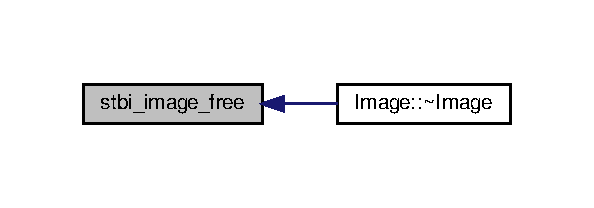
\includegraphics[width=285pt]{stb__image_8h_ad3e11bb44412a7ba348acfbad09caacb_icgraph}
\end{center}
\end{figure}
\mbox{\Hypertarget{stb__image_8h_aede708cca1304520b2afcf4d5eb61d70}\label{stb__image_8h_aede708cca1304520b2afcf4d5eb61d70}} 
\index{stb\+\_\+image.\+h@{stb\+\_\+image.\+h}!stbi\+\_\+info@{stbi\+\_\+info}}
\index{stbi\+\_\+info@{stbi\+\_\+info}!stb\+\_\+image.\+h@{stb\+\_\+image.\+h}}
\subsubsection{\texorpdfstring{stbi\+\_\+info()}{stbi\_info()}}
{\footnotesize\ttfamily \hyperlink{stb__image_8h_a2d9ec9850cd12aefe7641b456266a4c2}{S\+T\+B\+I\+D\+EF} int stbi\+\_\+info (\begin{DoxyParamCaption}\item[{char const $\ast$}]{filename,  }\item[{int $\ast$}]{x,  }\item[{int $\ast$}]{y,  }\item[{int $\ast$}]{comp }\end{DoxyParamCaption})}

\mbox{\Hypertarget{stb__image_8h_a86291c64cb663f41a34647d5e1abf363}\label{stb__image_8h_a86291c64cb663f41a34647d5e1abf363}} 
\index{stb\+\_\+image.\+h@{stb\+\_\+image.\+h}!stbi\+\_\+info\+\_\+from\+\_\+callbacks@{stbi\+\_\+info\+\_\+from\+\_\+callbacks}}
\index{stbi\+\_\+info\+\_\+from\+\_\+callbacks@{stbi\+\_\+info\+\_\+from\+\_\+callbacks}!stb\+\_\+image.\+h@{stb\+\_\+image.\+h}}
\subsubsection{\texorpdfstring{stbi\+\_\+info\+\_\+from\+\_\+callbacks()}{stbi\_info\_from\_callbacks()}}
{\footnotesize\ttfamily \hyperlink{stb__image_8h_a2d9ec9850cd12aefe7641b456266a4c2}{S\+T\+B\+I\+D\+EF} int stbi\+\_\+info\+\_\+from\+\_\+callbacks (\begin{DoxyParamCaption}\item[{\hyperlink{structstbi__io__callbacks}{stbi\+\_\+io\+\_\+callbacks} const $\ast$}]{clbk,  }\item[{void $\ast$}]{user,  }\item[{int $\ast$}]{x,  }\item[{int $\ast$}]{y,  }\item[{int $\ast$}]{comp }\end{DoxyParamCaption})}

\mbox{\Hypertarget{stb__image_8h_a28abedef4a0a93909332080df6be0021}\label{stb__image_8h_a28abedef4a0a93909332080df6be0021}} 
\index{stb\+\_\+image.\+h@{stb\+\_\+image.\+h}!stbi\+\_\+info\+\_\+from\+\_\+file@{stbi\+\_\+info\+\_\+from\+\_\+file}}
\index{stbi\+\_\+info\+\_\+from\+\_\+file@{stbi\+\_\+info\+\_\+from\+\_\+file}!stb\+\_\+image.\+h@{stb\+\_\+image.\+h}}
\subsubsection{\texorpdfstring{stbi\+\_\+info\+\_\+from\+\_\+file()}{stbi\_info\_from\_file()}}
{\footnotesize\ttfamily \hyperlink{stb__image_8h_a2d9ec9850cd12aefe7641b456266a4c2}{S\+T\+B\+I\+D\+EF} int stbi\+\_\+info\+\_\+from\+\_\+file (\begin{DoxyParamCaption}\item[{F\+I\+LE $\ast$}]{f,  }\item[{int $\ast$}]{x,  }\item[{int $\ast$}]{y,  }\item[{int $\ast$}]{comp }\end{DoxyParamCaption})}

\mbox{\Hypertarget{stb__image_8h_acfef077febce3bc3f1f339de478f3315}\label{stb__image_8h_acfef077febce3bc3f1f339de478f3315}} 
\index{stb\+\_\+image.\+h@{stb\+\_\+image.\+h}!stbi\+\_\+info\+\_\+from\+\_\+memory@{stbi\+\_\+info\+\_\+from\+\_\+memory}}
\index{stbi\+\_\+info\+\_\+from\+\_\+memory@{stbi\+\_\+info\+\_\+from\+\_\+memory}!stb\+\_\+image.\+h@{stb\+\_\+image.\+h}}
\subsubsection{\texorpdfstring{stbi\+\_\+info\+\_\+from\+\_\+memory()}{stbi\_info\_from\_memory()}}
{\footnotesize\ttfamily \hyperlink{stb__image_8h_a2d9ec9850cd12aefe7641b456266a4c2}{S\+T\+B\+I\+D\+EF} int stbi\+\_\+info\+\_\+from\+\_\+memory (\begin{DoxyParamCaption}\item[{\hyperlink{stb__image_8h_a28eb51a1512ce382ee50f20e1d04d50d}{stbi\+\_\+uc} const $\ast$}]{buffer,  }\item[{int}]{len,  }\item[{int $\ast$}]{x,  }\item[{int $\ast$}]{y,  }\item[{int $\ast$}]{comp }\end{DoxyParamCaption})}

\mbox{\Hypertarget{stb__image_8h_a7d9af55a35382c011cc186f7b62c00af}\label{stb__image_8h_a7d9af55a35382c011cc186f7b62c00af}} 
\index{stb\+\_\+image.\+h@{stb\+\_\+image.\+h}!stbi\+\_\+is\+\_\+16\+\_\+bit@{stbi\+\_\+is\+\_\+16\+\_\+bit}}
\index{stbi\+\_\+is\+\_\+16\+\_\+bit@{stbi\+\_\+is\+\_\+16\+\_\+bit}!stb\+\_\+image.\+h@{stb\+\_\+image.\+h}}
\subsubsection{\texorpdfstring{stbi\+\_\+is\+\_\+16\+\_\+bit()}{stbi\_is\_16\_bit()}}
{\footnotesize\ttfamily \hyperlink{stb__image_8h_a2d9ec9850cd12aefe7641b456266a4c2}{S\+T\+B\+I\+D\+EF} int stbi\+\_\+is\+\_\+16\+\_\+bit (\begin{DoxyParamCaption}\item[{char const $\ast$}]{filename }\end{DoxyParamCaption})}

\mbox{\Hypertarget{stb__image_8h_a990e0e38ab6e600bd9cbf5d30abd2f8f}\label{stb__image_8h_a990e0e38ab6e600bd9cbf5d30abd2f8f}} 
\index{stb\+\_\+image.\+h@{stb\+\_\+image.\+h}!stbi\+\_\+is\+\_\+16\+\_\+bit\+\_\+from\+\_\+callbacks@{stbi\+\_\+is\+\_\+16\+\_\+bit\+\_\+from\+\_\+callbacks}}
\index{stbi\+\_\+is\+\_\+16\+\_\+bit\+\_\+from\+\_\+callbacks@{stbi\+\_\+is\+\_\+16\+\_\+bit\+\_\+from\+\_\+callbacks}!stb\+\_\+image.\+h@{stb\+\_\+image.\+h}}
\subsubsection{\texorpdfstring{stbi\+\_\+is\+\_\+16\+\_\+bit\+\_\+from\+\_\+callbacks()}{stbi\_is\_16\_bit\_from\_callbacks()}}
{\footnotesize\ttfamily \hyperlink{stb__image_8h_a2d9ec9850cd12aefe7641b456266a4c2}{S\+T\+B\+I\+D\+EF} int stbi\+\_\+is\+\_\+16\+\_\+bit\+\_\+from\+\_\+callbacks (\begin{DoxyParamCaption}\item[{\hyperlink{structstbi__io__callbacks}{stbi\+\_\+io\+\_\+callbacks} const $\ast$}]{clbk,  }\item[{void $\ast$}]{user }\end{DoxyParamCaption})}

\mbox{\Hypertarget{stb__image_8h_a42fa266b80bfde22a0781ba2112d1c62}\label{stb__image_8h_a42fa266b80bfde22a0781ba2112d1c62}} 
\index{stb\+\_\+image.\+h@{stb\+\_\+image.\+h}!stbi\+\_\+is\+\_\+16\+\_\+bit\+\_\+from\+\_\+file@{stbi\+\_\+is\+\_\+16\+\_\+bit\+\_\+from\+\_\+file}}
\index{stbi\+\_\+is\+\_\+16\+\_\+bit\+\_\+from\+\_\+file@{stbi\+\_\+is\+\_\+16\+\_\+bit\+\_\+from\+\_\+file}!stb\+\_\+image.\+h@{stb\+\_\+image.\+h}}
\subsubsection{\texorpdfstring{stbi\+\_\+is\+\_\+16\+\_\+bit\+\_\+from\+\_\+file()}{stbi\_is\_16\_bit\_from\_file()}}
{\footnotesize\ttfamily \hyperlink{stb__image_8h_a2d9ec9850cd12aefe7641b456266a4c2}{S\+T\+B\+I\+D\+EF} int stbi\+\_\+is\+\_\+16\+\_\+bit\+\_\+from\+\_\+file (\begin{DoxyParamCaption}\item[{F\+I\+LE $\ast$}]{f }\end{DoxyParamCaption})}

\mbox{\Hypertarget{stb__image_8h_a548d486e07e0eb95671cb200d3a9530f}\label{stb__image_8h_a548d486e07e0eb95671cb200d3a9530f}} 
\index{stb\+\_\+image.\+h@{stb\+\_\+image.\+h}!stbi\+\_\+is\+\_\+16\+\_\+bit\+\_\+from\+\_\+memory@{stbi\+\_\+is\+\_\+16\+\_\+bit\+\_\+from\+\_\+memory}}
\index{stbi\+\_\+is\+\_\+16\+\_\+bit\+\_\+from\+\_\+memory@{stbi\+\_\+is\+\_\+16\+\_\+bit\+\_\+from\+\_\+memory}!stb\+\_\+image.\+h@{stb\+\_\+image.\+h}}
\subsubsection{\texorpdfstring{stbi\+\_\+is\+\_\+16\+\_\+bit\+\_\+from\+\_\+memory()}{stbi\_is\_16\_bit\_from\_memory()}}
{\footnotesize\ttfamily \hyperlink{stb__image_8h_a2d9ec9850cd12aefe7641b456266a4c2}{S\+T\+B\+I\+D\+EF} int stbi\+\_\+is\+\_\+16\+\_\+bit\+\_\+from\+\_\+memory (\begin{DoxyParamCaption}\item[{\hyperlink{stb__image_8h_a28eb51a1512ce382ee50f20e1d04d50d}{stbi\+\_\+uc} const $\ast$}]{buffer,  }\item[{int}]{len }\end{DoxyParamCaption})}

\mbox{\Hypertarget{stb__image_8h_ae70f9a302f7e87fd971075e7f758d55c}\label{stb__image_8h_ae70f9a302f7e87fd971075e7f758d55c}} 
\index{stb\+\_\+image.\+h@{stb\+\_\+image.\+h}!stbi\+\_\+is\+\_\+hdr@{stbi\+\_\+is\+\_\+hdr}}
\index{stbi\+\_\+is\+\_\+hdr@{stbi\+\_\+is\+\_\+hdr}!stb\+\_\+image.\+h@{stb\+\_\+image.\+h}}
\subsubsection{\texorpdfstring{stbi\+\_\+is\+\_\+hdr()}{stbi\_is\_hdr()}}
{\footnotesize\ttfamily \hyperlink{stb__image_8h_a2d9ec9850cd12aefe7641b456266a4c2}{S\+T\+B\+I\+D\+EF} int stbi\+\_\+is\+\_\+hdr (\begin{DoxyParamCaption}\item[{char const $\ast$}]{filename }\end{DoxyParamCaption})}

\mbox{\Hypertarget{stb__image_8h_af0e94f316fe1848f632517ca3c11d077}\label{stb__image_8h_af0e94f316fe1848f632517ca3c11d077}} 
\index{stb\+\_\+image.\+h@{stb\+\_\+image.\+h}!stbi\+\_\+is\+\_\+hdr\+\_\+from\+\_\+callbacks@{stbi\+\_\+is\+\_\+hdr\+\_\+from\+\_\+callbacks}}
\index{stbi\+\_\+is\+\_\+hdr\+\_\+from\+\_\+callbacks@{stbi\+\_\+is\+\_\+hdr\+\_\+from\+\_\+callbacks}!stb\+\_\+image.\+h@{stb\+\_\+image.\+h}}
\subsubsection{\texorpdfstring{stbi\+\_\+is\+\_\+hdr\+\_\+from\+\_\+callbacks()}{stbi\_is\_hdr\_from\_callbacks()}}
{\footnotesize\ttfamily \hyperlink{stb__image_8h_a2d9ec9850cd12aefe7641b456266a4c2}{S\+T\+B\+I\+D\+EF} int stbi\+\_\+is\+\_\+hdr\+\_\+from\+\_\+callbacks (\begin{DoxyParamCaption}\item[{\hyperlink{structstbi__io__callbacks}{stbi\+\_\+io\+\_\+callbacks} const $\ast$}]{clbk,  }\item[{void $\ast$}]{user }\end{DoxyParamCaption})}

\mbox{\Hypertarget{stb__image_8h_aaf10d41631e1e9214fde1688bdbd8524}\label{stb__image_8h_aaf10d41631e1e9214fde1688bdbd8524}} 
\index{stb\+\_\+image.\+h@{stb\+\_\+image.\+h}!stbi\+\_\+is\+\_\+hdr\+\_\+from\+\_\+file@{stbi\+\_\+is\+\_\+hdr\+\_\+from\+\_\+file}}
\index{stbi\+\_\+is\+\_\+hdr\+\_\+from\+\_\+file@{stbi\+\_\+is\+\_\+hdr\+\_\+from\+\_\+file}!stb\+\_\+image.\+h@{stb\+\_\+image.\+h}}
\subsubsection{\texorpdfstring{stbi\+\_\+is\+\_\+hdr\+\_\+from\+\_\+file()}{stbi\_is\_hdr\_from\_file()}}
{\footnotesize\ttfamily \hyperlink{stb__image_8h_a2d9ec9850cd12aefe7641b456266a4c2}{S\+T\+B\+I\+D\+EF} int stbi\+\_\+is\+\_\+hdr\+\_\+from\+\_\+file (\begin{DoxyParamCaption}\item[{F\+I\+LE $\ast$}]{f }\end{DoxyParamCaption})}

\mbox{\Hypertarget{stb__image_8h_a5cbc6f5cbb3b2d0d87ee959fcee9d23e}\label{stb__image_8h_a5cbc6f5cbb3b2d0d87ee959fcee9d23e}} 
\index{stb\+\_\+image.\+h@{stb\+\_\+image.\+h}!stbi\+\_\+is\+\_\+hdr\+\_\+from\+\_\+memory@{stbi\+\_\+is\+\_\+hdr\+\_\+from\+\_\+memory}}
\index{stbi\+\_\+is\+\_\+hdr\+\_\+from\+\_\+memory@{stbi\+\_\+is\+\_\+hdr\+\_\+from\+\_\+memory}!stb\+\_\+image.\+h@{stb\+\_\+image.\+h}}
\subsubsection{\texorpdfstring{stbi\+\_\+is\+\_\+hdr\+\_\+from\+\_\+memory()}{stbi\_is\_hdr\_from\_memory()}}
{\footnotesize\ttfamily \hyperlink{stb__image_8h_a2d9ec9850cd12aefe7641b456266a4c2}{S\+T\+B\+I\+D\+EF} int stbi\+\_\+is\+\_\+hdr\+\_\+from\+\_\+memory (\begin{DoxyParamCaption}\item[{\hyperlink{stb__image_8h_a28eb51a1512ce382ee50f20e1d04d50d}{stbi\+\_\+uc} const $\ast$}]{buffer,  }\item[{int}]{len }\end{DoxyParamCaption})}

\mbox{\Hypertarget{stb__image_8h_a1feccdcf726dcc6b5502e3efa85b7dbb}\label{stb__image_8h_a1feccdcf726dcc6b5502e3efa85b7dbb}} 
\index{stb\+\_\+image.\+h@{stb\+\_\+image.\+h}!stbi\+\_\+ldr\+\_\+to\+\_\+hdr\+\_\+gamma@{stbi\+\_\+ldr\+\_\+to\+\_\+hdr\+\_\+gamma}}
\index{stbi\+\_\+ldr\+\_\+to\+\_\+hdr\+\_\+gamma@{stbi\+\_\+ldr\+\_\+to\+\_\+hdr\+\_\+gamma}!stb\+\_\+image.\+h@{stb\+\_\+image.\+h}}
\subsubsection{\texorpdfstring{stbi\+\_\+ldr\+\_\+to\+\_\+hdr\+\_\+gamma()}{stbi\_ldr\_to\_hdr\_gamma()}}
{\footnotesize\ttfamily \hyperlink{stb__image_8h_a2d9ec9850cd12aefe7641b456266a4c2}{S\+T\+B\+I\+D\+EF} void stbi\+\_\+ldr\+\_\+to\+\_\+hdr\+\_\+gamma (\begin{DoxyParamCaption}\item[{float}]{gamma }\end{DoxyParamCaption})}

\mbox{\Hypertarget{stb__image_8h_af946583656a362a316b40c0421c20561}\label{stb__image_8h_af946583656a362a316b40c0421c20561}} 
\index{stb\+\_\+image.\+h@{stb\+\_\+image.\+h}!stbi\+\_\+ldr\+\_\+to\+\_\+hdr\+\_\+scale@{stbi\+\_\+ldr\+\_\+to\+\_\+hdr\+\_\+scale}}
\index{stbi\+\_\+ldr\+\_\+to\+\_\+hdr\+\_\+scale@{stbi\+\_\+ldr\+\_\+to\+\_\+hdr\+\_\+scale}!stb\+\_\+image.\+h@{stb\+\_\+image.\+h}}
\subsubsection{\texorpdfstring{stbi\+\_\+ldr\+\_\+to\+\_\+hdr\+\_\+scale()}{stbi\_ldr\_to\_hdr\_scale()}}
{\footnotesize\ttfamily \hyperlink{stb__image_8h_a2d9ec9850cd12aefe7641b456266a4c2}{S\+T\+B\+I\+D\+EF} void stbi\+\_\+ldr\+\_\+to\+\_\+hdr\+\_\+scale (\begin{DoxyParamCaption}\item[{float}]{scale }\end{DoxyParamCaption})}

\mbox{\Hypertarget{stb__image_8h_aefdc7387857a14894bbf321e9ea4f048}\label{stb__image_8h_aefdc7387857a14894bbf321e9ea4f048}} 
\index{stb\+\_\+image.\+h@{stb\+\_\+image.\+h}!stbi\+\_\+load@{stbi\+\_\+load}}
\index{stbi\+\_\+load@{stbi\+\_\+load}!stb\+\_\+image.\+h@{stb\+\_\+image.\+h}}
\subsubsection{\texorpdfstring{stbi\+\_\+load()}{stbi\_load()}}
{\footnotesize\ttfamily \hyperlink{stb__image_8h_a2d9ec9850cd12aefe7641b456266a4c2}{S\+T\+B\+I\+D\+EF} \hyperlink{stb__image_8h_a28eb51a1512ce382ee50f20e1d04d50d}{stbi\+\_\+uc}$\ast$ stbi\+\_\+load (\begin{DoxyParamCaption}\item[{char const $\ast$}]{filename,  }\item[{int $\ast$}]{x,  }\item[{int $\ast$}]{y,  }\item[{int $\ast$}]{channels\+\_\+in\+\_\+file,  }\item[{int}]{desired\+\_\+channels }\end{DoxyParamCaption})}

Here is the caller graph for this function\+:
\nopagebreak
\begin{figure}[H]
\begin{center}
\leavevmode
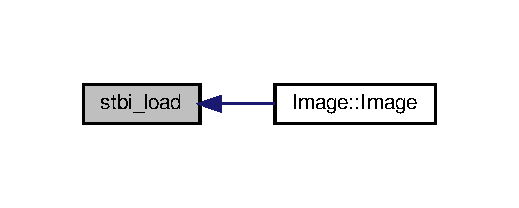
\includegraphics[width=249pt]{stb__image_8h_aefdc7387857a14894bbf321e9ea4f048_icgraph}
\end{center}
\end{figure}
\mbox{\Hypertarget{stb__image_8h_a8a58b6bcd805afa1bdb14f988dd37fee}\label{stb__image_8h_a8a58b6bcd805afa1bdb14f988dd37fee}} 
\index{stb\+\_\+image.\+h@{stb\+\_\+image.\+h}!stbi\+\_\+load\+\_\+16@{stbi\+\_\+load\+\_\+16}}
\index{stbi\+\_\+load\+\_\+16@{stbi\+\_\+load\+\_\+16}!stb\+\_\+image.\+h@{stb\+\_\+image.\+h}}
\subsubsection{\texorpdfstring{stbi\+\_\+load\+\_\+16()}{stbi\_load\_16()}}
{\footnotesize\ttfamily \hyperlink{stb__image_8h_a2d9ec9850cd12aefe7641b456266a4c2}{S\+T\+B\+I\+D\+EF} \hyperlink{stb__image_8h_a648037d4c55689328ba08c8f5d293df2}{stbi\+\_\+us}$\ast$ stbi\+\_\+load\+\_\+16 (\begin{DoxyParamCaption}\item[{char const $\ast$}]{filename,  }\item[{int $\ast$}]{x,  }\item[{int $\ast$}]{y,  }\item[{int $\ast$}]{channels\+\_\+in\+\_\+file,  }\item[{int}]{desired\+\_\+channels }\end{DoxyParamCaption})}

\mbox{\Hypertarget{stb__image_8h_a82bcc0957b6a4ebfdfa3d7f04fbaed18}\label{stb__image_8h_a82bcc0957b6a4ebfdfa3d7f04fbaed18}} 
\index{stb\+\_\+image.\+h@{stb\+\_\+image.\+h}!stbi\+\_\+load\+\_\+16\+\_\+from\+\_\+callbacks@{stbi\+\_\+load\+\_\+16\+\_\+from\+\_\+callbacks}}
\index{stbi\+\_\+load\+\_\+16\+\_\+from\+\_\+callbacks@{stbi\+\_\+load\+\_\+16\+\_\+from\+\_\+callbacks}!stb\+\_\+image.\+h@{stb\+\_\+image.\+h}}
\subsubsection{\texorpdfstring{stbi\+\_\+load\+\_\+16\+\_\+from\+\_\+callbacks()}{stbi\_load\_16\_from\_callbacks()}}
{\footnotesize\ttfamily \hyperlink{stb__image_8h_a2d9ec9850cd12aefe7641b456266a4c2}{S\+T\+B\+I\+D\+EF} \hyperlink{stb__image_8h_a648037d4c55689328ba08c8f5d293df2}{stbi\+\_\+us}$\ast$ stbi\+\_\+load\+\_\+16\+\_\+from\+\_\+callbacks (\begin{DoxyParamCaption}\item[{\hyperlink{structstbi__io__callbacks}{stbi\+\_\+io\+\_\+callbacks} const $\ast$}]{clbk,  }\item[{void $\ast$}]{user,  }\item[{int $\ast$}]{x,  }\item[{int $\ast$}]{y,  }\item[{int $\ast$}]{channels\+\_\+in\+\_\+file,  }\item[{int}]{desired\+\_\+channels }\end{DoxyParamCaption})}

\mbox{\Hypertarget{stb__image_8h_ad30fd870ed2138ce8f38c9dd29b2f76a}\label{stb__image_8h_ad30fd870ed2138ce8f38c9dd29b2f76a}} 
\index{stb\+\_\+image.\+h@{stb\+\_\+image.\+h}!stbi\+\_\+load\+\_\+16\+\_\+from\+\_\+memory@{stbi\+\_\+load\+\_\+16\+\_\+from\+\_\+memory}}
\index{stbi\+\_\+load\+\_\+16\+\_\+from\+\_\+memory@{stbi\+\_\+load\+\_\+16\+\_\+from\+\_\+memory}!stb\+\_\+image.\+h@{stb\+\_\+image.\+h}}
\subsubsection{\texorpdfstring{stbi\+\_\+load\+\_\+16\+\_\+from\+\_\+memory()}{stbi\_load\_16\_from\_memory()}}
{\footnotesize\ttfamily \hyperlink{stb__image_8h_a2d9ec9850cd12aefe7641b456266a4c2}{S\+T\+B\+I\+D\+EF} \hyperlink{stb__image_8h_a648037d4c55689328ba08c8f5d293df2}{stbi\+\_\+us}$\ast$ stbi\+\_\+load\+\_\+16\+\_\+from\+\_\+memory (\begin{DoxyParamCaption}\item[{\hyperlink{stb__image_8h_a28eb51a1512ce382ee50f20e1d04d50d}{stbi\+\_\+uc} const $\ast$}]{buffer,  }\item[{int}]{len,  }\item[{int $\ast$}]{x,  }\item[{int $\ast$}]{y,  }\item[{int $\ast$}]{channels\+\_\+in\+\_\+file,  }\item[{int}]{desired\+\_\+channels }\end{DoxyParamCaption})}

\mbox{\Hypertarget{stb__image_8h_a95ebc5c42c1a753200be8d465e933af7}\label{stb__image_8h_a95ebc5c42c1a753200be8d465e933af7}} 
\index{stb\+\_\+image.\+h@{stb\+\_\+image.\+h}!stbi\+\_\+load\+\_\+from\+\_\+callbacks@{stbi\+\_\+load\+\_\+from\+\_\+callbacks}}
\index{stbi\+\_\+load\+\_\+from\+\_\+callbacks@{stbi\+\_\+load\+\_\+from\+\_\+callbacks}!stb\+\_\+image.\+h@{stb\+\_\+image.\+h}}
\subsubsection{\texorpdfstring{stbi\+\_\+load\+\_\+from\+\_\+callbacks()}{stbi\_load\_from\_callbacks()}}
{\footnotesize\ttfamily \hyperlink{stb__image_8h_a2d9ec9850cd12aefe7641b456266a4c2}{S\+T\+B\+I\+D\+EF} \hyperlink{stb__image_8h_a28eb51a1512ce382ee50f20e1d04d50d}{stbi\+\_\+uc}$\ast$ stbi\+\_\+load\+\_\+from\+\_\+callbacks (\begin{DoxyParamCaption}\item[{\hyperlink{structstbi__io__callbacks}{stbi\+\_\+io\+\_\+callbacks} const $\ast$}]{clbk,  }\item[{void $\ast$}]{user,  }\item[{int $\ast$}]{x,  }\item[{int $\ast$}]{y,  }\item[{int $\ast$}]{channels\+\_\+in\+\_\+file,  }\item[{int}]{desired\+\_\+channels }\end{DoxyParamCaption})}

\mbox{\Hypertarget{stb__image_8h_aa9994764695597161e8f3776e97caa99}\label{stb__image_8h_aa9994764695597161e8f3776e97caa99}} 
\index{stb\+\_\+image.\+h@{stb\+\_\+image.\+h}!stbi\+\_\+load\+\_\+from\+\_\+file@{stbi\+\_\+load\+\_\+from\+\_\+file}}
\index{stbi\+\_\+load\+\_\+from\+\_\+file@{stbi\+\_\+load\+\_\+from\+\_\+file}!stb\+\_\+image.\+h@{stb\+\_\+image.\+h}}
\subsubsection{\texorpdfstring{stbi\+\_\+load\+\_\+from\+\_\+file()}{stbi\_load\_from\_file()}}
{\footnotesize\ttfamily \hyperlink{stb__image_8h_a2d9ec9850cd12aefe7641b456266a4c2}{S\+T\+B\+I\+D\+EF} \hyperlink{stb__image_8h_a28eb51a1512ce382ee50f20e1d04d50d}{stbi\+\_\+uc}$\ast$ stbi\+\_\+load\+\_\+from\+\_\+file (\begin{DoxyParamCaption}\item[{F\+I\+LE $\ast$}]{f,  }\item[{int $\ast$}]{x,  }\item[{int $\ast$}]{y,  }\item[{int $\ast$}]{channels\+\_\+in\+\_\+file,  }\item[{int}]{desired\+\_\+channels }\end{DoxyParamCaption})}

\mbox{\Hypertarget{stb__image_8h_a9ca2591f0987284129e82bf9dbcf7c6c}\label{stb__image_8h_a9ca2591f0987284129e82bf9dbcf7c6c}} 
\index{stb\+\_\+image.\+h@{stb\+\_\+image.\+h}!stbi\+\_\+load\+\_\+from\+\_\+file\+\_\+16@{stbi\+\_\+load\+\_\+from\+\_\+file\+\_\+16}}
\index{stbi\+\_\+load\+\_\+from\+\_\+file\+\_\+16@{stbi\+\_\+load\+\_\+from\+\_\+file\+\_\+16}!stb\+\_\+image.\+h@{stb\+\_\+image.\+h}}
\subsubsection{\texorpdfstring{stbi\+\_\+load\+\_\+from\+\_\+file\+\_\+16()}{stbi\_load\_from\_file\_16()}}
{\footnotesize\ttfamily \hyperlink{stb__image_8h_a2d9ec9850cd12aefe7641b456266a4c2}{S\+T\+B\+I\+D\+EF} \hyperlink{stb__image_8h_a648037d4c55689328ba08c8f5d293df2}{stbi\+\_\+us}$\ast$ stbi\+\_\+load\+\_\+from\+\_\+file\+\_\+16 (\begin{DoxyParamCaption}\item[{F\+I\+LE $\ast$}]{f,  }\item[{int $\ast$}]{x,  }\item[{int $\ast$}]{y,  }\item[{int $\ast$}]{channels\+\_\+in\+\_\+file,  }\item[{int}]{desired\+\_\+channels }\end{DoxyParamCaption})}

\mbox{\Hypertarget{stb__image_8h_acae25d31bfae29d75482f07fecf2935f}\label{stb__image_8h_acae25d31bfae29d75482f07fecf2935f}} 
\index{stb\+\_\+image.\+h@{stb\+\_\+image.\+h}!stbi\+\_\+load\+\_\+from\+\_\+memory@{stbi\+\_\+load\+\_\+from\+\_\+memory}}
\index{stbi\+\_\+load\+\_\+from\+\_\+memory@{stbi\+\_\+load\+\_\+from\+\_\+memory}!stb\+\_\+image.\+h@{stb\+\_\+image.\+h}}
\subsubsection{\texorpdfstring{stbi\+\_\+load\+\_\+from\+\_\+memory()}{stbi\_load\_from\_memory()}}
{\footnotesize\ttfamily \hyperlink{stb__image_8h_a2d9ec9850cd12aefe7641b456266a4c2}{S\+T\+B\+I\+D\+EF} \hyperlink{stb__image_8h_a28eb51a1512ce382ee50f20e1d04d50d}{stbi\+\_\+uc}$\ast$ stbi\+\_\+load\+\_\+from\+\_\+memory (\begin{DoxyParamCaption}\item[{\hyperlink{stb__image_8h_a28eb51a1512ce382ee50f20e1d04d50d}{stbi\+\_\+uc} const $\ast$}]{buffer,  }\item[{int}]{len,  }\item[{int $\ast$}]{x,  }\item[{int $\ast$}]{y,  }\item[{int $\ast$}]{channels\+\_\+in\+\_\+file,  }\item[{int}]{desired\+\_\+channels }\end{DoxyParamCaption})}

\mbox{\Hypertarget{stb__image_8h_ab81ccbc3526368d651117ef48df82b01}\label{stb__image_8h_ab81ccbc3526368d651117ef48df82b01}} 
\index{stb\+\_\+image.\+h@{stb\+\_\+image.\+h}!stbi\+\_\+load\+\_\+gif\+\_\+from\+\_\+memory@{stbi\+\_\+load\+\_\+gif\+\_\+from\+\_\+memory}}
\index{stbi\+\_\+load\+\_\+gif\+\_\+from\+\_\+memory@{stbi\+\_\+load\+\_\+gif\+\_\+from\+\_\+memory}!stb\+\_\+image.\+h@{stb\+\_\+image.\+h}}
\subsubsection{\texorpdfstring{stbi\+\_\+load\+\_\+gif\+\_\+from\+\_\+memory()}{stbi\_load\_gif\_from\_memory()}}
{\footnotesize\ttfamily \hyperlink{stb__image_8h_a2d9ec9850cd12aefe7641b456266a4c2}{S\+T\+B\+I\+D\+EF} \hyperlink{stb__image_8h_a28eb51a1512ce382ee50f20e1d04d50d}{stbi\+\_\+uc}$\ast$ stbi\+\_\+load\+\_\+gif\+\_\+from\+\_\+memory (\begin{DoxyParamCaption}\item[{\hyperlink{stb__image_8h_a28eb51a1512ce382ee50f20e1d04d50d}{stbi\+\_\+uc} const $\ast$}]{buffer,  }\item[{int}]{len,  }\item[{int $\ast$$\ast$}]{delays,  }\item[{int $\ast$}]{x,  }\item[{int $\ast$}]{y,  }\item[{int $\ast$}]{z,  }\item[{int $\ast$}]{comp,  }\item[{int}]{req\+\_\+comp }\end{DoxyParamCaption})}

\mbox{\Hypertarget{stb__image_8h_af4f17acd30945a75901fdc022f90575f}\label{stb__image_8h_af4f17acd30945a75901fdc022f90575f}} 
\index{stb\+\_\+image.\+h@{stb\+\_\+image.\+h}!stbi\+\_\+loadf@{stbi\+\_\+loadf}}
\index{stbi\+\_\+loadf@{stbi\+\_\+loadf}!stb\+\_\+image.\+h@{stb\+\_\+image.\+h}}
\subsubsection{\texorpdfstring{stbi\+\_\+loadf()}{stbi\_loadf()}}
{\footnotesize\ttfamily \hyperlink{stb__image_8h_a2d9ec9850cd12aefe7641b456266a4c2}{S\+T\+B\+I\+D\+EF} float$\ast$ stbi\+\_\+loadf (\begin{DoxyParamCaption}\item[{char const $\ast$}]{filename,  }\item[{int $\ast$}]{x,  }\item[{int $\ast$}]{y,  }\item[{int $\ast$}]{channels\+\_\+in\+\_\+file,  }\item[{int}]{desired\+\_\+channels }\end{DoxyParamCaption})}

\mbox{\Hypertarget{stb__image_8h_a6e7fd261af79ecef2208df3a6cc806bb}\label{stb__image_8h_a6e7fd261af79ecef2208df3a6cc806bb}} 
\index{stb\+\_\+image.\+h@{stb\+\_\+image.\+h}!stbi\+\_\+loadf\+\_\+from\+\_\+callbacks@{stbi\+\_\+loadf\+\_\+from\+\_\+callbacks}}
\index{stbi\+\_\+loadf\+\_\+from\+\_\+callbacks@{stbi\+\_\+loadf\+\_\+from\+\_\+callbacks}!stb\+\_\+image.\+h@{stb\+\_\+image.\+h}}
\subsubsection{\texorpdfstring{stbi\+\_\+loadf\+\_\+from\+\_\+callbacks()}{stbi\_loadf\_from\_callbacks()}}
{\footnotesize\ttfamily \hyperlink{stb__image_8h_a2d9ec9850cd12aefe7641b456266a4c2}{S\+T\+B\+I\+D\+EF} float$\ast$ stbi\+\_\+loadf\+\_\+from\+\_\+callbacks (\begin{DoxyParamCaption}\item[{\hyperlink{structstbi__io__callbacks}{stbi\+\_\+io\+\_\+callbacks} const $\ast$}]{clbk,  }\item[{void $\ast$}]{user,  }\item[{int $\ast$}]{x,  }\item[{int $\ast$}]{y,  }\item[{int $\ast$}]{channels\+\_\+in\+\_\+file,  }\item[{int}]{desired\+\_\+channels }\end{DoxyParamCaption})}

\mbox{\Hypertarget{stb__image_8h_ace82446ecd7b5c760cde062179660f46}\label{stb__image_8h_ace82446ecd7b5c760cde062179660f46}} 
\index{stb\+\_\+image.\+h@{stb\+\_\+image.\+h}!stbi\+\_\+loadf\+\_\+from\+\_\+file@{stbi\+\_\+loadf\+\_\+from\+\_\+file}}
\index{stbi\+\_\+loadf\+\_\+from\+\_\+file@{stbi\+\_\+loadf\+\_\+from\+\_\+file}!stb\+\_\+image.\+h@{stb\+\_\+image.\+h}}
\subsubsection{\texorpdfstring{stbi\+\_\+loadf\+\_\+from\+\_\+file()}{stbi\_loadf\_from\_file()}}
{\footnotesize\ttfamily \hyperlink{stb__image_8h_a2d9ec9850cd12aefe7641b456266a4c2}{S\+T\+B\+I\+D\+EF} float$\ast$ stbi\+\_\+loadf\+\_\+from\+\_\+file (\begin{DoxyParamCaption}\item[{F\+I\+LE $\ast$}]{f,  }\item[{int $\ast$}]{x,  }\item[{int $\ast$}]{y,  }\item[{int $\ast$}]{channels\+\_\+in\+\_\+file,  }\item[{int}]{desired\+\_\+channels }\end{DoxyParamCaption})}

\mbox{\Hypertarget{stb__image_8h_a5d47fb76ce1e34eb0729ad932c9c48e2}\label{stb__image_8h_a5d47fb76ce1e34eb0729ad932c9c48e2}} 
\index{stb\+\_\+image.\+h@{stb\+\_\+image.\+h}!stbi\+\_\+loadf\+\_\+from\+\_\+memory@{stbi\+\_\+loadf\+\_\+from\+\_\+memory}}
\index{stbi\+\_\+loadf\+\_\+from\+\_\+memory@{stbi\+\_\+loadf\+\_\+from\+\_\+memory}!stb\+\_\+image.\+h@{stb\+\_\+image.\+h}}
\subsubsection{\texorpdfstring{stbi\+\_\+loadf\+\_\+from\+\_\+memory()}{stbi\_loadf\_from\_memory()}}
{\footnotesize\ttfamily \hyperlink{stb__image_8h_a2d9ec9850cd12aefe7641b456266a4c2}{S\+T\+B\+I\+D\+EF} float$\ast$ stbi\+\_\+loadf\+\_\+from\+\_\+memory (\begin{DoxyParamCaption}\item[{\hyperlink{stb__image_8h_a28eb51a1512ce382ee50f20e1d04d50d}{stbi\+\_\+uc} const $\ast$}]{buffer,  }\item[{int}]{len,  }\item[{int $\ast$}]{x,  }\item[{int $\ast$}]{y,  }\item[{int $\ast$}]{channels\+\_\+in\+\_\+file,  }\item[{int}]{desired\+\_\+channels }\end{DoxyParamCaption})}

\mbox{\Hypertarget{stb__image_8h_ab89c177fc52f1bb2dc1c05e48129a0a4}\label{stb__image_8h_ab89c177fc52f1bb2dc1c05e48129a0a4}} 
\index{stb\+\_\+image.\+h@{stb\+\_\+image.\+h}!stbi\+\_\+set\+\_\+flip\+\_\+vertically\+\_\+on\+\_\+load@{stbi\+\_\+set\+\_\+flip\+\_\+vertically\+\_\+on\+\_\+load}}
\index{stbi\+\_\+set\+\_\+flip\+\_\+vertically\+\_\+on\+\_\+load@{stbi\+\_\+set\+\_\+flip\+\_\+vertically\+\_\+on\+\_\+load}!stb\+\_\+image.\+h@{stb\+\_\+image.\+h}}
\subsubsection{\texorpdfstring{stbi\+\_\+set\+\_\+flip\+\_\+vertically\+\_\+on\+\_\+load()}{stbi\_set\_flip\_vertically\_on\_load()}}
{\footnotesize\ttfamily \hyperlink{stb__image_8h_a2d9ec9850cd12aefe7641b456266a4c2}{S\+T\+B\+I\+D\+EF} void stbi\+\_\+set\+\_\+flip\+\_\+vertically\+\_\+on\+\_\+load (\begin{DoxyParamCaption}\item[{int}]{flag\+\_\+true\+\_\+if\+\_\+should\+\_\+flip }\end{DoxyParamCaption})}

\mbox{\Hypertarget{stb__image_8h_ad683202a3f6ec89729b5ad9220ae98ee}\label{stb__image_8h_ad683202a3f6ec89729b5ad9220ae98ee}} 
\index{stb\+\_\+image.\+h@{stb\+\_\+image.\+h}!stbi\+\_\+set\+\_\+flip\+\_\+vertically\+\_\+on\+\_\+load\+\_\+thread@{stbi\+\_\+set\+\_\+flip\+\_\+vertically\+\_\+on\+\_\+load\+\_\+thread}}
\index{stbi\+\_\+set\+\_\+flip\+\_\+vertically\+\_\+on\+\_\+load\+\_\+thread@{stbi\+\_\+set\+\_\+flip\+\_\+vertically\+\_\+on\+\_\+load\+\_\+thread}!stb\+\_\+image.\+h@{stb\+\_\+image.\+h}}
\subsubsection{\texorpdfstring{stbi\+\_\+set\+\_\+flip\+\_\+vertically\+\_\+on\+\_\+load\+\_\+thread()}{stbi\_set\_flip\_vertically\_on\_load\_thread()}}
{\footnotesize\ttfamily \hyperlink{stb__image_8h_a2d9ec9850cd12aefe7641b456266a4c2}{S\+T\+B\+I\+D\+EF} void stbi\+\_\+set\+\_\+flip\+\_\+vertically\+\_\+on\+\_\+load\+\_\+thread (\begin{DoxyParamCaption}\item[{int}]{flag\+\_\+true\+\_\+if\+\_\+should\+\_\+flip }\end{DoxyParamCaption})}

\mbox{\Hypertarget{stb__image_8h_a3f02e0053e1c8d08a3ed436e6a82c7c9}\label{stb__image_8h_a3f02e0053e1c8d08a3ed436e6a82c7c9}} 
\index{stb\+\_\+image.\+h@{stb\+\_\+image.\+h}!stbi\+\_\+set\+\_\+unpremultiply\+\_\+on\+\_\+load@{stbi\+\_\+set\+\_\+unpremultiply\+\_\+on\+\_\+load}}
\index{stbi\+\_\+set\+\_\+unpremultiply\+\_\+on\+\_\+load@{stbi\+\_\+set\+\_\+unpremultiply\+\_\+on\+\_\+load}!stb\+\_\+image.\+h@{stb\+\_\+image.\+h}}
\subsubsection{\texorpdfstring{stbi\+\_\+set\+\_\+unpremultiply\+\_\+on\+\_\+load()}{stbi\_set\_unpremultiply\_on\_load()}}
{\footnotesize\ttfamily \hyperlink{stb__image_8h_a2d9ec9850cd12aefe7641b456266a4c2}{S\+T\+B\+I\+D\+EF} void stbi\+\_\+set\+\_\+unpremultiply\+\_\+on\+\_\+load (\begin{DoxyParamCaption}\item[{int}]{flag\+\_\+true\+\_\+if\+\_\+should\+\_\+unpremultiply }\end{DoxyParamCaption})}

\mbox{\Hypertarget{stb__image_8h_ae8447830c49bc17f8491e12c1f0ded48}\label{stb__image_8h_ae8447830c49bc17f8491e12c1f0ded48}} 
\index{stb\+\_\+image.\+h@{stb\+\_\+image.\+h}!stbi\+\_\+zlib\+\_\+decode\+\_\+buffer@{stbi\+\_\+zlib\+\_\+decode\+\_\+buffer}}
\index{stbi\+\_\+zlib\+\_\+decode\+\_\+buffer@{stbi\+\_\+zlib\+\_\+decode\+\_\+buffer}!stb\+\_\+image.\+h@{stb\+\_\+image.\+h}}
\subsubsection{\texorpdfstring{stbi\+\_\+zlib\+\_\+decode\+\_\+buffer()}{stbi\_zlib\_decode\_buffer()}}
{\footnotesize\ttfamily \hyperlink{stb__image_8h_a2d9ec9850cd12aefe7641b456266a4c2}{S\+T\+B\+I\+D\+EF} int stbi\+\_\+zlib\+\_\+decode\+\_\+buffer (\begin{DoxyParamCaption}\item[{char $\ast$}]{obuffer,  }\item[{int}]{olen,  }\item[{const char $\ast$}]{ibuffer,  }\item[{int}]{ilen }\end{DoxyParamCaption})}

\mbox{\Hypertarget{stb__image_8h_a4919b67b12e0e3acc5301f185ca77e2e}\label{stb__image_8h_a4919b67b12e0e3acc5301f185ca77e2e}} 
\index{stb\+\_\+image.\+h@{stb\+\_\+image.\+h}!stbi\+\_\+zlib\+\_\+decode\+\_\+malloc@{stbi\+\_\+zlib\+\_\+decode\+\_\+malloc}}
\index{stbi\+\_\+zlib\+\_\+decode\+\_\+malloc@{stbi\+\_\+zlib\+\_\+decode\+\_\+malloc}!stb\+\_\+image.\+h@{stb\+\_\+image.\+h}}
\subsubsection{\texorpdfstring{stbi\+\_\+zlib\+\_\+decode\+\_\+malloc()}{stbi\_zlib\_decode\_malloc()}}
{\footnotesize\ttfamily \hyperlink{stb__image_8h_a2d9ec9850cd12aefe7641b456266a4c2}{S\+T\+B\+I\+D\+EF} char$\ast$ stbi\+\_\+zlib\+\_\+decode\+\_\+malloc (\begin{DoxyParamCaption}\item[{const char $\ast$}]{buffer,  }\item[{int}]{len,  }\item[{int $\ast$}]{outlen }\end{DoxyParamCaption})}

\mbox{\Hypertarget{stb__image_8h_aaaa17a529bec51403cc23dc2e7c36d79}\label{stb__image_8h_aaaa17a529bec51403cc23dc2e7c36d79}} 
\index{stb\+\_\+image.\+h@{stb\+\_\+image.\+h}!stbi\+\_\+zlib\+\_\+decode\+\_\+malloc\+\_\+guesssize@{stbi\+\_\+zlib\+\_\+decode\+\_\+malloc\+\_\+guesssize}}
\index{stbi\+\_\+zlib\+\_\+decode\+\_\+malloc\+\_\+guesssize@{stbi\+\_\+zlib\+\_\+decode\+\_\+malloc\+\_\+guesssize}!stb\+\_\+image.\+h@{stb\+\_\+image.\+h}}
\subsubsection{\texorpdfstring{stbi\+\_\+zlib\+\_\+decode\+\_\+malloc\+\_\+guesssize()}{stbi\_zlib\_decode\_malloc\_guesssize()}}
{\footnotesize\ttfamily \hyperlink{stb__image_8h_a2d9ec9850cd12aefe7641b456266a4c2}{S\+T\+B\+I\+D\+EF} char$\ast$ stbi\+\_\+zlib\+\_\+decode\+\_\+malloc\+\_\+guesssize (\begin{DoxyParamCaption}\item[{const char $\ast$}]{buffer,  }\item[{int}]{len,  }\item[{int}]{initial\+\_\+size,  }\item[{int $\ast$}]{outlen }\end{DoxyParamCaption})}

\mbox{\Hypertarget{stb__image_8h_a038b0e741859a482b8b9d60167e54d27}\label{stb__image_8h_a038b0e741859a482b8b9d60167e54d27}} 
\index{stb\+\_\+image.\+h@{stb\+\_\+image.\+h}!stbi\+\_\+zlib\+\_\+decode\+\_\+malloc\+\_\+guesssize\+\_\+headerflag@{stbi\+\_\+zlib\+\_\+decode\+\_\+malloc\+\_\+guesssize\+\_\+headerflag}}
\index{stbi\+\_\+zlib\+\_\+decode\+\_\+malloc\+\_\+guesssize\+\_\+headerflag@{stbi\+\_\+zlib\+\_\+decode\+\_\+malloc\+\_\+guesssize\+\_\+headerflag}!stb\+\_\+image.\+h@{stb\+\_\+image.\+h}}
\subsubsection{\texorpdfstring{stbi\+\_\+zlib\+\_\+decode\+\_\+malloc\+\_\+guesssize\+\_\+headerflag()}{stbi\_zlib\_decode\_malloc\_guesssize\_headerflag()}}
{\footnotesize\ttfamily \hyperlink{stb__image_8h_a2d9ec9850cd12aefe7641b456266a4c2}{S\+T\+B\+I\+D\+EF} char$\ast$ stbi\+\_\+zlib\+\_\+decode\+\_\+malloc\+\_\+guesssize\+\_\+headerflag (\begin{DoxyParamCaption}\item[{const char $\ast$}]{buffer,  }\item[{int}]{len,  }\item[{int}]{initial\+\_\+size,  }\item[{int $\ast$}]{outlen,  }\item[{int}]{parse\+\_\+header }\end{DoxyParamCaption})}

\mbox{\Hypertarget{stb__image_8h_a0d12efc011adfff7521f3b924feb0b0e}\label{stb__image_8h_a0d12efc011adfff7521f3b924feb0b0e}} 
\index{stb\+\_\+image.\+h@{stb\+\_\+image.\+h}!stbi\+\_\+zlib\+\_\+decode\+\_\+noheader\+\_\+buffer@{stbi\+\_\+zlib\+\_\+decode\+\_\+noheader\+\_\+buffer}}
\index{stbi\+\_\+zlib\+\_\+decode\+\_\+noheader\+\_\+buffer@{stbi\+\_\+zlib\+\_\+decode\+\_\+noheader\+\_\+buffer}!stb\+\_\+image.\+h@{stb\+\_\+image.\+h}}
\subsubsection{\texorpdfstring{stbi\+\_\+zlib\+\_\+decode\+\_\+noheader\+\_\+buffer()}{stbi\_zlib\_decode\_noheader\_buffer()}}
{\footnotesize\ttfamily \hyperlink{stb__image_8h_a2d9ec9850cd12aefe7641b456266a4c2}{S\+T\+B\+I\+D\+EF} int stbi\+\_\+zlib\+\_\+decode\+\_\+noheader\+\_\+buffer (\begin{DoxyParamCaption}\item[{char $\ast$}]{obuffer,  }\item[{int}]{olen,  }\item[{const char $\ast$}]{ibuffer,  }\item[{int}]{ilen }\end{DoxyParamCaption})}

\mbox{\Hypertarget{stb__image_8h_a7fbd65c83495f13f22469fe493775739}\label{stb__image_8h_a7fbd65c83495f13f22469fe493775739}} 
\index{stb\+\_\+image.\+h@{stb\+\_\+image.\+h}!stbi\+\_\+zlib\+\_\+decode\+\_\+noheader\+\_\+malloc@{stbi\+\_\+zlib\+\_\+decode\+\_\+noheader\+\_\+malloc}}
\index{stbi\+\_\+zlib\+\_\+decode\+\_\+noheader\+\_\+malloc@{stbi\+\_\+zlib\+\_\+decode\+\_\+noheader\+\_\+malloc}!stb\+\_\+image.\+h@{stb\+\_\+image.\+h}}
\subsubsection{\texorpdfstring{stbi\+\_\+zlib\+\_\+decode\+\_\+noheader\+\_\+malloc()}{stbi\_zlib\_decode\_noheader\_malloc()}}
{\footnotesize\ttfamily \hyperlink{stb__image_8h_a2d9ec9850cd12aefe7641b456266a4c2}{S\+T\+B\+I\+D\+EF} char$\ast$ stbi\+\_\+zlib\+\_\+decode\+\_\+noheader\+\_\+malloc (\begin{DoxyParamCaption}\item[{const char $\ast$}]{buffer,  }\item[{int}]{len,  }\item[{int $\ast$}]{outlen }\end{DoxyParamCaption})}


\hypertarget{stb__image__write_8h}{}\doxysection{inc/stb\+\_\+image\+\_\+write.h File Reference}
\label{stb__image__write_8h}\index{inc/stb\_image\_write.h@{inc/stb\_image\_write.h}}
{\ttfamily \#include $<$stdlib.\+h$>$}\newline
Include dependency graph for stb\+\_\+image\+\_\+write.\+h\+:
% FIG 0
This graph shows which files directly or indirectly include this file\+:
% FIG 1
\doxysubsection*{Macros}
\begin{DoxyCompactItemize}
\item 
\#define \mbox{\hyperlink{stb__image__write_8h_a1d964457ebf7cc898b8cb14e66cbfaa8}{S\+T\+B\+I\+W\+D\+EF}}~extern
\end{DoxyCompactItemize}
\doxysubsection*{Typedefs}
\begin{DoxyCompactItemize}
\item 
typedef void \mbox{\hyperlink{stb__image__write_8h_a2326fd2fd79095b9ef34695a0bda114f}{stbi\+\_\+write\+\_\+func}}(void $\ast$context, void $\ast$data, int size)
\end{DoxyCompactItemize}
\doxysubsection*{Functions}
\begin{DoxyCompactItemize}
\item 
\mbox{\hyperlink{stb__image__write_8h_a1d964457ebf7cc898b8cb14e66cbfaa8}{S\+T\+B\+I\+W\+D\+EF}} int \mbox{\hyperlink{stb__image__write_8h_a9c03e5171f6aea47fde6dafcf3249ccf}{stbi\+\_\+write\+\_\+png}} (char const $\ast$filename, int w, int h, int comp, const void $\ast$data, int stride\+\_\+in\+\_\+bytes)
\item 
\mbox{\hyperlink{stb__image__write_8h_a1d964457ebf7cc898b8cb14e66cbfaa8}{S\+T\+B\+I\+W\+D\+EF}} int \mbox{\hyperlink{stb__image__write_8h_a4f63ec842984e5db3edf2da89f16038e}{stbi\+\_\+write\+\_\+bmp}} (char const $\ast$filename, int w, int h, int comp, const void $\ast$data)
\item 
\mbox{\hyperlink{stb__image__write_8h_a1d964457ebf7cc898b8cb14e66cbfaa8}{S\+T\+B\+I\+W\+D\+EF}} int \mbox{\hyperlink{stb__image__write_8h_ab7a84427c6d7e894090fbeae3bc8f6da}{stbi\+\_\+write\+\_\+tga}} (char const $\ast$filename, int w, int h, int comp, const void $\ast$data)
\item 
\mbox{\hyperlink{stb__image__write_8h_a1d964457ebf7cc898b8cb14e66cbfaa8}{S\+T\+B\+I\+W\+D\+EF}} int \mbox{\hyperlink{stb__image__write_8h_a21f22be0194761e08b682ed543ef6161}{stbi\+\_\+write\+\_\+hdr}} (char const $\ast$filename, int w, int h, int comp, const float $\ast$data)
\item 
\mbox{\hyperlink{stb__image__write_8h_a1d964457ebf7cc898b8cb14e66cbfaa8}{S\+T\+B\+I\+W\+D\+EF}} int \mbox{\hyperlink{stb__image__write_8h_a41048e8f918179d2788284ef9cc2590c}{stbi\+\_\+write\+\_\+jpg}} (char const $\ast$filename, int x, int y, int comp, const void $\ast$data, int quality)
\item 
\mbox{\hyperlink{stb__image__write_8h_a1d964457ebf7cc898b8cb14e66cbfaa8}{S\+T\+B\+I\+W\+D\+EF}} int \mbox{\hyperlink{stb__image__write_8h_a72dcd18698d64c92082449912c39a4e5}{stbi\+\_\+write\+\_\+png\+\_\+to\+\_\+func}} (\mbox{\hyperlink{stb__image__write_8h_a2326fd2fd79095b9ef34695a0bda114f}{stbi\+\_\+write\+\_\+func}} $\ast$func, void $\ast$context, int w, int h, int comp, const void $\ast$data, int stride\+\_\+in\+\_\+bytes)
\item 
\mbox{\hyperlink{stb__image__write_8h_a1d964457ebf7cc898b8cb14e66cbfaa8}{S\+T\+B\+I\+W\+D\+EF}} int \mbox{\hyperlink{stb__image__write_8h_aca9573665994b2244a6a045b2a1df1ea}{stbi\+\_\+write\+\_\+bmp\+\_\+to\+\_\+func}} (\mbox{\hyperlink{stb__image__write_8h_a2326fd2fd79095b9ef34695a0bda114f}{stbi\+\_\+write\+\_\+func}} $\ast$func, void $\ast$context, int w, int h, int comp, const void $\ast$data)
\item 
\mbox{\hyperlink{stb__image__write_8h_a1d964457ebf7cc898b8cb14e66cbfaa8}{S\+T\+B\+I\+W\+D\+EF}} int \mbox{\hyperlink{stb__image__write_8h_a5e5c6483c1d45a65fe208f52937cd315}{stbi\+\_\+write\+\_\+tga\+\_\+to\+\_\+func}} (\mbox{\hyperlink{stb__image__write_8h_a2326fd2fd79095b9ef34695a0bda114f}{stbi\+\_\+write\+\_\+func}} $\ast$func, void $\ast$context, int w, int h, int comp, const void $\ast$data)
\item 
\mbox{\hyperlink{stb__image__write_8h_a1d964457ebf7cc898b8cb14e66cbfaa8}{S\+T\+B\+I\+W\+D\+EF}} int \mbox{\hyperlink{stb__image__write_8h_ac9214f775162b61a3503c76875966c11}{stbi\+\_\+write\+\_\+hdr\+\_\+to\+\_\+func}} (\mbox{\hyperlink{stb__image__write_8h_a2326fd2fd79095b9ef34695a0bda114f}{stbi\+\_\+write\+\_\+func}} $\ast$func, void $\ast$context, int w, int h, int comp, const float $\ast$data)
\item 
\mbox{\hyperlink{stb__image__write_8h_a1d964457ebf7cc898b8cb14e66cbfaa8}{S\+T\+B\+I\+W\+D\+EF}} int \mbox{\hyperlink{stb__image__write_8h_afbe60a9afbcbd6d54f98f72afd46a676}{stbi\+\_\+write\+\_\+jpg\+\_\+to\+\_\+func}} (\mbox{\hyperlink{stb__image__write_8h_a2326fd2fd79095b9ef34695a0bda114f}{stbi\+\_\+write\+\_\+func}} $\ast$func, void $\ast$context, int x, int y, int comp, const void $\ast$data, int quality)
\item 
\mbox{\hyperlink{stb__image__write_8h_a1d964457ebf7cc898b8cb14e66cbfaa8}{S\+T\+B\+I\+W\+D\+EF}} void \mbox{\hyperlink{stb__image__write_8h_a5c41a5d16dc665edd2489b982ba29b85}{stbi\+\_\+flip\+\_\+vertically\+\_\+on\+\_\+write}} (int flip\+\_\+boolean)
\end{DoxyCompactItemize}
\doxysubsection*{Variables}
\begin{DoxyCompactItemize}
\item 
int \mbox{\hyperlink{stb__image__write_8h_a7aa69838d830bd1e917b2a20d2030e0c}{stbi\+\_\+write\+\_\+tga\+\_\+with\+\_\+rle}}
\item 
int \mbox{\hyperlink{stb__image__write_8h_ac40d349d241f781ed7b621259ce2b3c2}{stbi\+\_\+write\+\_\+png\+\_\+compression\+\_\+level}}
\item 
int \mbox{\hyperlink{stb__image__write_8h_acfc7bbb01f0c4f6079727cfa1b086912}{stbi\+\_\+write\+\_\+force\+\_\+png\+\_\+filter}}
\end{DoxyCompactItemize}


\doxysubsection{Macro Definition Documentation}
\mbox{\Hypertarget{stb__image__write_8h_a1d964457ebf7cc898b8cb14e66cbfaa8}\label{stb__image__write_8h_a1d964457ebf7cc898b8cb14e66cbfaa8}} 
\index{stb\_image\_write.h@{stb\_image\_write.h}!STBIWDEF@{STBIWDEF}}
\index{STBIWDEF@{STBIWDEF}!stb\_image\_write.h@{stb\_image\_write.h}}
\doxysubsubsection{\texorpdfstring{STBIWDEF}{STBIWDEF}}
{\footnotesize\ttfamily \#define S\+T\+B\+I\+W\+D\+EF~extern}



\doxysubsection{Typedef Documentation}
\mbox{\Hypertarget{stb__image__write_8h_a2326fd2fd79095b9ef34695a0bda114f}\label{stb__image__write_8h_a2326fd2fd79095b9ef34695a0bda114f}} 
\index{stb\_image\_write.h@{stb\_image\_write.h}!stbi\_write\_func@{stbi\_write\_func}}
\index{stbi\_write\_func@{stbi\_write\_func}!stb\_image\_write.h@{stb\_image\_write.h}}
\doxysubsubsection{\texorpdfstring{stbi\_write\_func}{stbi\_write\_func}}
{\footnotesize\ttfamily typedef void stbi\+\_\+write\+\_\+func(void $\ast$context, void $\ast$data, int size)}



\doxysubsection{Function Documentation}
\mbox{\Hypertarget{stb__image__write_8h_a5c41a5d16dc665edd2489b982ba29b85}\label{stb__image__write_8h_a5c41a5d16dc665edd2489b982ba29b85}} 
\index{stb\_image\_write.h@{stb\_image\_write.h}!stbi\_flip\_vertically\_on\_write@{stbi\_flip\_vertically\_on\_write}}
\index{stbi\_flip\_vertically\_on\_write@{stbi\_flip\_vertically\_on\_write}!stb\_image\_write.h@{stb\_image\_write.h}}
\doxysubsubsection{\texorpdfstring{stbi\_flip\_vertically\_on\_write()}{stbi\_flip\_vertically\_on\_write()}}
{\footnotesize\ttfamily \mbox{\hyperlink{stb__image__write_8h_a1d964457ebf7cc898b8cb14e66cbfaa8}{S\+T\+B\+I\+W\+D\+EF}} void stbi\+\_\+flip\+\_\+vertically\+\_\+on\+\_\+write (\begin{DoxyParamCaption}\item[{int}]{flip\+\_\+boolean }\end{DoxyParamCaption})}

\mbox{\Hypertarget{stb__image__write_8h_a4f63ec842984e5db3edf2da89f16038e}\label{stb__image__write_8h_a4f63ec842984e5db3edf2da89f16038e}} 
\index{stb\_image\_write.h@{stb\_image\_write.h}!stbi\_write\_bmp@{stbi\_write\_bmp}}
\index{stbi\_write\_bmp@{stbi\_write\_bmp}!stb\_image\_write.h@{stb\_image\_write.h}}
\doxysubsubsection{\texorpdfstring{stbi\_write\_bmp()}{stbi\_write\_bmp()}}
{\footnotesize\ttfamily \mbox{\hyperlink{stb__image__write_8h_a1d964457ebf7cc898b8cb14e66cbfaa8}{S\+T\+B\+I\+W\+D\+EF}} int stbi\+\_\+write\+\_\+bmp (\begin{DoxyParamCaption}\item[{char const $\ast$}]{filename,  }\item[{int}]{w,  }\item[{int}]{h,  }\item[{int}]{comp,  }\item[{const void $\ast$}]{data }\end{DoxyParamCaption})}

\mbox{\Hypertarget{stb__image__write_8h_aca9573665994b2244a6a045b2a1df1ea}\label{stb__image__write_8h_aca9573665994b2244a6a045b2a1df1ea}} 
\index{stb\_image\_write.h@{stb\_image\_write.h}!stbi\_write\_bmp\_to\_func@{stbi\_write\_bmp\_to\_func}}
\index{stbi\_write\_bmp\_to\_func@{stbi\_write\_bmp\_to\_func}!stb\_image\_write.h@{stb\_image\_write.h}}
\doxysubsubsection{\texorpdfstring{stbi\_write\_bmp\_to\_func()}{stbi\_write\_bmp\_to\_func()}}
{\footnotesize\ttfamily \mbox{\hyperlink{stb__image__write_8h_a1d964457ebf7cc898b8cb14e66cbfaa8}{S\+T\+B\+I\+W\+D\+EF}} int stbi\+\_\+write\+\_\+bmp\+\_\+to\+\_\+func (\begin{DoxyParamCaption}\item[{\mbox{\hyperlink{stb__image__write_8h_a2326fd2fd79095b9ef34695a0bda114f}{stbi\+\_\+write\+\_\+func}} $\ast$}]{func,  }\item[{void $\ast$}]{context,  }\item[{int}]{w,  }\item[{int}]{h,  }\item[{int}]{comp,  }\item[{const void $\ast$}]{data }\end{DoxyParamCaption})}

\mbox{\Hypertarget{stb__image__write_8h_a21f22be0194761e08b682ed543ef6161}\label{stb__image__write_8h_a21f22be0194761e08b682ed543ef6161}} 
\index{stb\_image\_write.h@{stb\_image\_write.h}!stbi\_write\_hdr@{stbi\_write\_hdr}}
\index{stbi\_write\_hdr@{stbi\_write\_hdr}!stb\_image\_write.h@{stb\_image\_write.h}}
\doxysubsubsection{\texorpdfstring{stbi\_write\_hdr()}{stbi\_write\_hdr()}}
{\footnotesize\ttfamily \mbox{\hyperlink{stb__image__write_8h_a1d964457ebf7cc898b8cb14e66cbfaa8}{S\+T\+B\+I\+W\+D\+EF}} int stbi\+\_\+write\+\_\+hdr (\begin{DoxyParamCaption}\item[{char const $\ast$}]{filename,  }\item[{int}]{w,  }\item[{int}]{h,  }\item[{int}]{comp,  }\item[{const float $\ast$}]{data }\end{DoxyParamCaption})}

\mbox{\Hypertarget{stb__image__write_8h_ac9214f775162b61a3503c76875966c11}\label{stb__image__write_8h_ac9214f775162b61a3503c76875966c11}} 
\index{stb\_image\_write.h@{stb\_image\_write.h}!stbi\_write\_hdr\_to\_func@{stbi\_write\_hdr\_to\_func}}
\index{stbi\_write\_hdr\_to\_func@{stbi\_write\_hdr\_to\_func}!stb\_image\_write.h@{stb\_image\_write.h}}
\doxysubsubsection{\texorpdfstring{stbi\_write\_hdr\_to\_func()}{stbi\_write\_hdr\_to\_func()}}
{\footnotesize\ttfamily \mbox{\hyperlink{stb__image__write_8h_a1d964457ebf7cc898b8cb14e66cbfaa8}{S\+T\+B\+I\+W\+D\+EF}} int stbi\+\_\+write\+\_\+hdr\+\_\+to\+\_\+func (\begin{DoxyParamCaption}\item[{\mbox{\hyperlink{stb__image__write_8h_a2326fd2fd79095b9ef34695a0bda114f}{stbi\+\_\+write\+\_\+func}} $\ast$}]{func,  }\item[{void $\ast$}]{context,  }\item[{int}]{w,  }\item[{int}]{h,  }\item[{int}]{comp,  }\item[{const float $\ast$}]{data }\end{DoxyParamCaption})}

\mbox{\Hypertarget{stb__image__write_8h_a41048e8f918179d2788284ef9cc2590c}\label{stb__image__write_8h_a41048e8f918179d2788284ef9cc2590c}} 
\index{stb\_image\_write.h@{stb\_image\_write.h}!stbi\_write\_jpg@{stbi\_write\_jpg}}
\index{stbi\_write\_jpg@{stbi\_write\_jpg}!stb\_image\_write.h@{stb\_image\_write.h}}
\doxysubsubsection{\texorpdfstring{stbi\_write\_jpg()}{stbi\_write\_jpg()}}
{\footnotesize\ttfamily \mbox{\hyperlink{stb__image__write_8h_a1d964457ebf7cc898b8cb14e66cbfaa8}{S\+T\+B\+I\+W\+D\+EF}} int stbi\+\_\+write\+\_\+jpg (\begin{DoxyParamCaption}\item[{char const $\ast$}]{filename,  }\item[{int}]{x,  }\item[{int}]{y,  }\item[{int}]{comp,  }\item[{const void $\ast$}]{data,  }\item[{int}]{quality }\end{DoxyParamCaption})}

Here is the caller graph for this function\+:
% FIG 2
\mbox{\Hypertarget{stb__image__write_8h_afbe60a9afbcbd6d54f98f72afd46a676}\label{stb__image__write_8h_afbe60a9afbcbd6d54f98f72afd46a676}} 
\index{stb\_image\_write.h@{stb\_image\_write.h}!stbi\_write\_jpg\_to\_func@{stbi\_write\_jpg\_to\_func}}
\index{stbi\_write\_jpg\_to\_func@{stbi\_write\_jpg\_to\_func}!stb\_image\_write.h@{stb\_image\_write.h}}
\doxysubsubsection{\texorpdfstring{stbi\_write\_jpg\_to\_func()}{stbi\_write\_jpg\_to\_func()}}
{\footnotesize\ttfamily \mbox{\hyperlink{stb__image__write_8h_a1d964457ebf7cc898b8cb14e66cbfaa8}{S\+T\+B\+I\+W\+D\+EF}} int stbi\+\_\+write\+\_\+jpg\+\_\+to\+\_\+func (\begin{DoxyParamCaption}\item[{\mbox{\hyperlink{stb__image__write_8h_a2326fd2fd79095b9ef34695a0bda114f}{stbi\+\_\+write\+\_\+func}} $\ast$}]{func,  }\item[{void $\ast$}]{context,  }\item[{int}]{x,  }\item[{int}]{y,  }\item[{int}]{comp,  }\item[{const void $\ast$}]{data,  }\item[{int}]{quality }\end{DoxyParamCaption})}

\mbox{\Hypertarget{stb__image__write_8h_a9c03e5171f6aea47fde6dafcf3249ccf}\label{stb__image__write_8h_a9c03e5171f6aea47fde6dafcf3249ccf}} 
\index{stb\_image\_write.h@{stb\_image\_write.h}!stbi\_write\_png@{stbi\_write\_png}}
\index{stbi\_write\_png@{stbi\_write\_png}!stb\_image\_write.h@{stb\_image\_write.h}}
\doxysubsubsection{\texorpdfstring{stbi\_write\_png()}{stbi\_write\_png()}}
{\footnotesize\ttfamily \mbox{\hyperlink{stb__image__write_8h_a1d964457ebf7cc898b8cb14e66cbfaa8}{S\+T\+B\+I\+W\+D\+EF}} int stbi\+\_\+write\+\_\+png (\begin{DoxyParamCaption}\item[{char const $\ast$}]{filename,  }\item[{int}]{w,  }\item[{int}]{h,  }\item[{int}]{comp,  }\item[{const void $\ast$}]{data,  }\item[{int}]{stride\+\_\+in\+\_\+bytes }\end{DoxyParamCaption})}

Here is the caller graph for this function\+:
% FIG 3
\mbox{\Hypertarget{stb__image__write_8h_a72dcd18698d64c92082449912c39a4e5}\label{stb__image__write_8h_a72dcd18698d64c92082449912c39a4e5}} 
\index{stb\_image\_write.h@{stb\_image\_write.h}!stbi\_write\_png\_to\_func@{stbi\_write\_png\_to\_func}}
\index{stbi\_write\_png\_to\_func@{stbi\_write\_png\_to\_func}!stb\_image\_write.h@{stb\_image\_write.h}}
\doxysubsubsection{\texorpdfstring{stbi\_write\_png\_to\_func()}{stbi\_write\_png\_to\_func()}}
{\footnotesize\ttfamily \mbox{\hyperlink{stb__image__write_8h_a1d964457ebf7cc898b8cb14e66cbfaa8}{S\+T\+B\+I\+W\+D\+EF}} int stbi\+\_\+write\+\_\+png\+\_\+to\+\_\+func (\begin{DoxyParamCaption}\item[{\mbox{\hyperlink{stb__image__write_8h_a2326fd2fd79095b9ef34695a0bda114f}{stbi\+\_\+write\+\_\+func}} $\ast$}]{func,  }\item[{void $\ast$}]{context,  }\item[{int}]{w,  }\item[{int}]{h,  }\item[{int}]{comp,  }\item[{const void $\ast$}]{data,  }\item[{int}]{stride\+\_\+in\+\_\+bytes }\end{DoxyParamCaption})}

\mbox{\Hypertarget{stb__image__write_8h_ab7a84427c6d7e894090fbeae3bc8f6da}\label{stb__image__write_8h_ab7a84427c6d7e894090fbeae3bc8f6da}} 
\index{stb\_image\_write.h@{stb\_image\_write.h}!stbi\_write\_tga@{stbi\_write\_tga}}
\index{stbi\_write\_tga@{stbi\_write\_tga}!stb\_image\_write.h@{stb\_image\_write.h}}
\doxysubsubsection{\texorpdfstring{stbi\_write\_tga()}{stbi\_write\_tga()}}
{\footnotesize\ttfamily \mbox{\hyperlink{stb__image__write_8h_a1d964457ebf7cc898b8cb14e66cbfaa8}{S\+T\+B\+I\+W\+D\+EF}} int stbi\+\_\+write\+\_\+tga (\begin{DoxyParamCaption}\item[{char const $\ast$}]{filename,  }\item[{int}]{w,  }\item[{int}]{h,  }\item[{int}]{comp,  }\item[{const void $\ast$}]{data }\end{DoxyParamCaption})}

\mbox{\Hypertarget{stb__image__write_8h_a5e5c6483c1d45a65fe208f52937cd315}\label{stb__image__write_8h_a5e5c6483c1d45a65fe208f52937cd315}} 
\index{stb\_image\_write.h@{stb\_image\_write.h}!stbi\_write\_tga\_to\_func@{stbi\_write\_tga\_to\_func}}
\index{stbi\_write\_tga\_to\_func@{stbi\_write\_tga\_to\_func}!stb\_image\_write.h@{stb\_image\_write.h}}
\doxysubsubsection{\texorpdfstring{stbi\_write\_tga\_to\_func()}{stbi\_write\_tga\_to\_func()}}
{\footnotesize\ttfamily \mbox{\hyperlink{stb__image__write_8h_a1d964457ebf7cc898b8cb14e66cbfaa8}{S\+T\+B\+I\+W\+D\+EF}} int stbi\+\_\+write\+\_\+tga\+\_\+to\+\_\+func (\begin{DoxyParamCaption}\item[{\mbox{\hyperlink{stb__image__write_8h_a2326fd2fd79095b9ef34695a0bda114f}{stbi\+\_\+write\+\_\+func}} $\ast$}]{func,  }\item[{void $\ast$}]{context,  }\item[{int}]{w,  }\item[{int}]{h,  }\item[{int}]{comp,  }\item[{const void $\ast$}]{data }\end{DoxyParamCaption})}



\doxysubsection{Variable Documentation}
\mbox{\Hypertarget{stb__image__write_8h_acfc7bbb01f0c4f6079727cfa1b086912}\label{stb__image__write_8h_acfc7bbb01f0c4f6079727cfa1b086912}} 
\index{stb\_image\_write.h@{stb\_image\_write.h}!stbi\_write\_force\_png\_filter@{stbi\_write\_force\_png\_filter}}
\index{stbi\_write\_force\_png\_filter@{stbi\_write\_force\_png\_filter}!stb\_image\_write.h@{stb\_image\_write.h}}
\doxysubsubsection{\texorpdfstring{stbi\_write\_force\_png\_filter}{stbi\_write\_force\_png\_filter}}
{\footnotesize\ttfamily int stbi\+\_\+write\+\_\+force\+\_\+png\+\_\+filter}

\mbox{\Hypertarget{stb__image__write_8h_ac40d349d241f781ed7b621259ce2b3c2}\label{stb__image__write_8h_ac40d349d241f781ed7b621259ce2b3c2}} 
\index{stb\_image\_write.h@{stb\_image\_write.h}!stbi\_write\_png\_compression\_level@{stbi\_write\_png\_compression\_level}}
\index{stbi\_write\_png\_compression\_level@{stbi\_write\_png\_compression\_level}!stb\_image\_write.h@{stb\_image\_write.h}}
\doxysubsubsection{\texorpdfstring{stbi\_write\_png\_compression\_level}{stbi\_write\_png\_compression\_level}}
{\footnotesize\ttfamily int stbi\+\_\+write\+\_\+png\+\_\+compression\+\_\+level}

\mbox{\Hypertarget{stb__image__write_8h_a7aa69838d830bd1e917b2a20d2030e0c}\label{stb__image__write_8h_a7aa69838d830bd1e917b2a20d2030e0c}} 
\index{stb\_image\_write.h@{stb\_image\_write.h}!stbi\_write\_tga\_with\_rle@{stbi\_write\_tga\_with\_rle}}
\index{stbi\_write\_tga\_with\_rle@{stbi\_write\_tga\_with\_rle}!stb\_image\_write.h@{stb\_image\_write.h}}
\doxysubsubsection{\texorpdfstring{stbi\_write\_tga\_with\_rle}{stbi\_write\_tga\_with\_rle}}
{\footnotesize\ttfamily int stbi\+\_\+write\+\_\+tga\+\_\+with\+\_\+rle}


\hypertarget{glad_8c}{}\doxysection{src/glad.c File Reference}
\label{glad_8c}\index{src/glad.c@{src/glad.c}}
{\ttfamily \#include $<$stdio.\+h$>$}\newline
{\ttfamily \#include $<$stdlib.\+h$>$}\newline
{\ttfamily \#include $<$string.\+h$>$}\newline
{\ttfamily \#include $<$glad/glad.\+h$>$}\newline
{\ttfamily \#include $<$dlfcn.\+h$>$}\newline
Include dependency graph for glad.\+c\+:
% FIG 0
\doxysubsection*{Typedefs}
\begin{DoxyCompactItemize}
\item 
typedef void $\ast$A\+P\+I\+E\+N\+T\+R\+YP \mbox{\hyperlink{glad_8c_aca765b78242406adec0d1614c5d7036b}{P\+F\+N\+G\+L\+X\+G\+E\+T\+P\+R\+O\+C\+A\+D\+D\+R\+E\+S\+S\+P\+R\+O\+C\+\_\+\+P\+R\+I\+V\+A\+TE}}(const char $\ast$)
\end{DoxyCompactItemize}
\doxysubsection*{Functions}
\begin{DoxyCompactItemize}
\item 
static void $\ast$ \mbox{\hyperlink{glad_8c_ad63f2bf7c845fd310286b42a454ba71d}{get\+\_\+proc}} (const char $\ast$namez)
\item 
static int \mbox{\hyperlink{glad_8c_a538b0e09de5780f026ad62462fade0a6}{open\+\_\+gl}} (void)
\item 
static void \mbox{\hyperlink{glad_8c_aa3222c9728bc7f7846f3e684b440a030}{close\+\_\+gl}} ()
\item 
int \mbox{\hyperlink{glad_8c_a137453294a2756a898902ef399b3d437}{glad\+Load\+GL}} (void)
\item 
static int \mbox{\hyperlink{glad_8c_abfb50eb07d43a6e366811edf9feff173}{get\+\_\+exts}} (void)
\item 
static void \mbox{\hyperlink{glad_8c_a250a03ed54f517313be3fb311c1d0929}{free\+\_\+exts}} (void)
\item 
static int \mbox{\hyperlink{glad_8c_abfdc555a06ed44e71045a703a7d43951}{has\+\_\+ext}} (const char $\ast$ext)
\item 
static void \mbox{\hyperlink{glad_8c_ac9cefadc8a6c809297856b3cb546d1d4}{load\+\_\+\+G\+L\+\_\+\+V\+E\+R\+S\+I\+O\+N\+\_\+1\+\_\+0}} (G\+L\+A\+Dloadproc load)
\item 
static void \mbox{\hyperlink{glad_8c_a35dbc78b11773681adc60e990fef7005}{load\+\_\+\+G\+L\+\_\+\+V\+E\+R\+S\+I\+O\+N\+\_\+1\+\_\+1}} (G\+L\+A\+Dloadproc load)
\item 
static void \mbox{\hyperlink{glad_8c_a577c4b9e1351249c243b007ecc4a975e}{load\+\_\+\+G\+L\+\_\+\+V\+E\+R\+S\+I\+O\+N\+\_\+1\+\_\+2}} (G\+L\+A\+Dloadproc load)
\item 
static void \mbox{\hyperlink{glad_8c_a64db1ca3b160134bd85d5121be77ab1c}{load\+\_\+\+G\+L\+\_\+\+V\+E\+R\+S\+I\+O\+N\+\_\+1\+\_\+3}} (G\+L\+A\+Dloadproc load)
\item 
static void \mbox{\hyperlink{glad_8c_a3fcc343e68a41abbf2aaf2898ba6c662}{load\+\_\+\+G\+L\+\_\+\+V\+E\+R\+S\+I\+O\+N\+\_\+1\+\_\+4}} (G\+L\+A\+Dloadproc load)
\item 
static void \mbox{\hyperlink{glad_8c_a5b8a4ead1fe41911c78f289e1e099c17}{load\+\_\+\+G\+L\+\_\+\+V\+E\+R\+S\+I\+O\+N\+\_\+1\+\_\+5}} (G\+L\+A\+Dloadproc load)
\item 
static void \mbox{\hyperlink{glad_8c_ada4838bbc696bf9bd3fee9945ae2fc62}{load\+\_\+\+G\+L\+\_\+\+V\+E\+R\+S\+I\+O\+N\+\_\+2\+\_\+0}} (G\+L\+A\+Dloadproc load)
\item 
static void \mbox{\hyperlink{glad_8c_a6b1ddad462fc87b8ca81a8228c81bf9f}{load\+\_\+\+G\+L\+\_\+\+V\+E\+R\+S\+I\+O\+N\+\_\+2\+\_\+1}} (G\+L\+A\+Dloadproc load)
\item 
static void \mbox{\hyperlink{glad_8c_a66fb68f92ff5be9c41e8fd9e3a0f1f22}{load\+\_\+\+G\+L\+\_\+\+V\+E\+R\+S\+I\+O\+N\+\_\+3\+\_\+0}} (G\+L\+A\+Dloadproc load)
\item 
static void \mbox{\hyperlink{glad_8c_aa0161dc921d58866d5c9384b365bfae7}{load\+\_\+\+G\+L\+\_\+\+V\+E\+R\+S\+I\+O\+N\+\_\+3\+\_\+1}} (G\+L\+A\+Dloadproc load)
\item 
static void \mbox{\hyperlink{glad_8c_aa4ad9ec346eeec0578169e552b802662}{load\+\_\+\+G\+L\+\_\+\+V\+E\+R\+S\+I\+O\+N\+\_\+3\+\_\+2}} (G\+L\+A\+Dloadproc load)
\item 
static void \mbox{\hyperlink{glad_8c_a5b35a05be99645aebc78627b564fb0be}{load\+\_\+\+G\+L\+\_\+\+V\+E\+R\+S\+I\+O\+N\+\_\+3\+\_\+3}} (G\+L\+A\+Dloadproc load)
\item 
static void \mbox{\hyperlink{glad_8c_afd687e92ccc3435db99eb010fc5565a4}{load\+\_\+\+G\+L\+\_\+\+V\+E\+R\+S\+I\+O\+N\+\_\+4\+\_\+0}} (G\+L\+A\+Dloadproc load)
\item 
static void \mbox{\hyperlink{glad_8c_ab46b2b729425b5bb92c402e7b08c90fa}{load\+\_\+\+G\+L\+\_\+\+V\+E\+R\+S\+I\+O\+N\+\_\+4\+\_\+1}} (G\+L\+A\+Dloadproc load)
\item 
static void \mbox{\hyperlink{glad_8c_a34c73452306d56278046dd284ec050bd}{load\+\_\+\+G\+L\+\_\+\+V\+E\+R\+S\+I\+O\+N\+\_\+4\+\_\+2}} (G\+L\+A\+Dloadproc load)
\item 
static void \mbox{\hyperlink{glad_8c_ac96c85fb3086e40f55ecc2a85e88f940}{load\+\_\+\+G\+L\+\_\+\+V\+E\+R\+S\+I\+O\+N\+\_\+4\+\_\+3}} (G\+L\+A\+Dloadproc load)
\item 
static void \mbox{\hyperlink{glad_8c_a3379f8fef4545548f7508288d9f23d91}{load\+\_\+\+G\+L\+\_\+\+V\+E\+R\+S\+I\+O\+N\+\_\+4\+\_\+4}} (G\+L\+A\+Dloadproc load)
\item 
static void \mbox{\hyperlink{glad_8c_a09519edf390523b7e1eda978dc24fc0e}{load\+\_\+\+G\+L\+\_\+\+V\+E\+R\+S\+I\+O\+N\+\_\+4\+\_\+5}} (G\+L\+A\+Dloadproc load)
\item 
static void \mbox{\hyperlink{glad_8c_a19a87c3f49eec57840b60e259a1f009f}{load\+\_\+\+G\+L\+\_\+\+V\+E\+R\+S\+I\+O\+N\+\_\+4\+\_\+6}} (G\+L\+A\+Dloadproc load)
\item 
static int \mbox{\hyperlink{glad_8c_aec888869187731b49111dfbea5f7cd56}{find\+\_\+extensions\+GL}} (void)
\item 
static void \mbox{\hyperlink{glad_8c_a1e6b94e667c5087bcd17801e4e4942a3}{find\+\_\+core\+GL}} (void)
\item 
int \mbox{\hyperlink{glad_8c_af70e4674f75bd3bbfedf7979607c65ef}{glad\+Load\+G\+L\+Loader}} (G\+L\+A\+Dloadproc load)
\end{DoxyCompactItemize}
\doxysubsection*{Variables}
\begin{DoxyCompactItemize}
\item 
static void $\ast$ \mbox{\hyperlink{glad_8c_a3c299869dbd023d474ce0f8d7d77a09a}{lib\+GL}}
\item 
static \mbox{\hyperlink{glad_8c_aca765b78242406adec0d1614c5d7036b}{P\+F\+N\+G\+L\+X\+G\+E\+T\+P\+R\+O\+C\+A\+D\+D\+R\+E\+S\+S\+P\+R\+O\+C\+\_\+\+P\+R\+I\+V\+A\+TE}} \mbox{\hyperlink{glad_8c_a533ffb590d3a069e5d568eb898c1f251}{glad\+Get\+Proc\+Address\+Ptr}}
\item 
struct glad\+G\+Lversion\+Struct \mbox{\hyperlink{glad_8c_a936871a0ece33eb83e12fe9a0b19aec5}{G\+L\+Version}}
\item 
static int \mbox{\hyperlink{glad_8c_a9e504bd5bf1cd6a49e3a76a33a58ede4}{max\+\_\+loaded\+\_\+major}}
\item 
static int \mbox{\hyperlink{glad_8c_ad98d2ec0df0b5d1256e056d8d663980e}{max\+\_\+loaded\+\_\+minor}}
\item 
static const char $\ast$ \mbox{\hyperlink{glad_8c_a866827ab8f22713c7232944595e94906}{exts}} = N\+U\+LL
\item 
static int \mbox{\hyperlink{glad_8c_afa6e943e56556f413c9720e419157252}{num\+\_\+exts\+\_\+i}} = 0
\item 
static const char $\ast$$\ast$ \mbox{\hyperlink{glad_8c_a08801e74281bbcbf8a58ac37ddd1def8}{exts\+\_\+i}} = N\+U\+LL
\item 
int \mbox{\hyperlink{glad_8c_a36ca5b6d392d79f489283e35c4f59886}{G\+L\+A\+D\+\_\+\+G\+L\+\_\+\+V\+E\+R\+S\+I\+O\+N\+\_\+1\+\_\+0}}
\item 
int \mbox{\hyperlink{glad_8c_a72f5c2c53a25a3411a9d3d1ec595a445}{G\+L\+A\+D\+\_\+\+G\+L\+\_\+\+V\+E\+R\+S\+I\+O\+N\+\_\+1\+\_\+1}}
\item 
int \mbox{\hyperlink{glad_8c_a98446be7f32ba314c20ce8f1887c1a6e}{G\+L\+A\+D\+\_\+\+G\+L\+\_\+\+V\+E\+R\+S\+I\+O\+N\+\_\+1\+\_\+2}}
\item 
int \mbox{\hyperlink{glad_8c_a7d5a1046898057af127a76b4ebda642e}{G\+L\+A\+D\+\_\+\+G\+L\+\_\+\+V\+E\+R\+S\+I\+O\+N\+\_\+1\+\_\+3}}
\item 
int \mbox{\hyperlink{glad_8c_ab467084103b9bf0fadf0285ba3b2be92}{G\+L\+A\+D\+\_\+\+G\+L\+\_\+\+V\+E\+R\+S\+I\+O\+N\+\_\+1\+\_\+4}}
\item 
int \mbox{\hyperlink{glad_8c_a3e0a29fb94488db80914f358a986c1a0}{G\+L\+A\+D\+\_\+\+G\+L\+\_\+\+V\+E\+R\+S\+I\+O\+N\+\_\+1\+\_\+5}}
\item 
int \mbox{\hyperlink{glad_8c_a40f63cf24bf7c1b2b921b2a592a0ef99}{G\+L\+A\+D\+\_\+\+G\+L\+\_\+\+V\+E\+R\+S\+I\+O\+N\+\_\+2\+\_\+0}}
\item 
int \mbox{\hyperlink{glad_8c_af3e324557ab88547818471d65dc5d57e}{G\+L\+A\+D\+\_\+\+G\+L\+\_\+\+V\+E\+R\+S\+I\+O\+N\+\_\+2\+\_\+1}}
\item 
int \mbox{\hyperlink{glad_8c_a60c438fb96d9b4c9d1bfc63ed2f610d3}{G\+L\+A\+D\+\_\+\+G\+L\+\_\+\+V\+E\+R\+S\+I\+O\+N\+\_\+3\+\_\+0}}
\item 
int \mbox{\hyperlink{glad_8c_aa8877d647b8e1cef3fa39a6cb1286d5a}{G\+L\+A\+D\+\_\+\+G\+L\+\_\+\+V\+E\+R\+S\+I\+O\+N\+\_\+3\+\_\+1}}
\item 
int \mbox{\hyperlink{glad_8c_a32681a519ad91af0a441b63253a6f10f}{G\+L\+A\+D\+\_\+\+G\+L\+\_\+\+V\+E\+R\+S\+I\+O\+N\+\_\+3\+\_\+2}}
\item 
int \mbox{\hyperlink{glad_8c_a67fc3be6cd6075c41297d05d12320692}{G\+L\+A\+D\+\_\+\+G\+L\+\_\+\+V\+E\+R\+S\+I\+O\+N\+\_\+3\+\_\+3}}
\item 
int \mbox{\hyperlink{glad_8c_a815c7b5ff43e808b7895710146932b0e}{G\+L\+A\+D\+\_\+\+G\+L\+\_\+\+V\+E\+R\+S\+I\+O\+N\+\_\+4\+\_\+0}}
\item 
int \mbox{\hyperlink{glad_8c_af40ffa850cab45bf8d666cc002052a43}{G\+L\+A\+D\+\_\+\+G\+L\+\_\+\+V\+E\+R\+S\+I\+O\+N\+\_\+4\+\_\+1}}
\item 
int \mbox{\hyperlink{glad_8c_adaa47c948e30299906ba7a8a2355ed56}{G\+L\+A\+D\+\_\+\+G\+L\+\_\+\+V\+E\+R\+S\+I\+O\+N\+\_\+4\+\_\+2}}
\item 
int \mbox{\hyperlink{glad_8c_aa9bf131c977959b96973bc4229c49a7b}{G\+L\+A\+D\+\_\+\+G\+L\+\_\+\+V\+E\+R\+S\+I\+O\+N\+\_\+4\+\_\+3}}
\item 
int \mbox{\hyperlink{glad_8c_a63e726f8184d07e39c891b98ed00f925}{G\+L\+A\+D\+\_\+\+G\+L\+\_\+\+V\+E\+R\+S\+I\+O\+N\+\_\+4\+\_\+4}}
\item 
int \mbox{\hyperlink{glad_8c_a8d9b47e5f80eaae4169eaeb2888b8b6d}{G\+L\+A\+D\+\_\+\+G\+L\+\_\+\+V\+E\+R\+S\+I\+O\+N\+\_\+4\+\_\+5}}
\item 
int \mbox{\hyperlink{glad_8c_ad2a6812c71eb238d5b5d1f7b9759d432}{G\+L\+A\+D\+\_\+\+G\+L\+\_\+\+V\+E\+R\+S\+I\+O\+N\+\_\+4\+\_\+6}}
\item 
P\+F\+N\+G\+L\+C\+O\+P\+Y\+T\+E\+X\+I\+M\+A\+G\+E1\+D\+P\+R\+OC \mbox{\hyperlink{glad_8c_a0a289a129835507246162c06574461aa}{glad\+\_\+gl\+Copy\+Tex\+Image1D}}
\item 
P\+F\+N\+G\+L\+T\+E\+X\+T\+U\+R\+E\+P\+A\+R\+A\+M\+E\+T\+E\+R\+F\+P\+R\+OC \mbox{\hyperlink{glad_8c_af483a34a65ab9beb79404a0b3c3bbc4d}{glad\+\_\+gl\+Texture\+Parameterf}}
\item 
P\+F\+N\+G\+L\+V\+E\+R\+T\+E\+X\+A\+T\+T\+R\+I\+B\+I3\+U\+I\+P\+R\+OC \mbox{\hyperlink{glad_8c_a67091dfa47c0878563d0378bde55c55e}{glad\+\_\+gl\+Vertex\+Attrib\+I3ui}}
\item 
P\+F\+N\+G\+L\+V\+E\+R\+T\+E\+X\+A\+R\+R\+A\+Y\+E\+L\+E\+M\+E\+N\+T\+B\+U\+F\+F\+E\+R\+P\+R\+OC \mbox{\hyperlink{glad_8c_a66da58c7466c85010e90bcf0654f7025}{glad\+\_\+gl\+Vertex\+Array\+Element\+Buffer}}
\item 
P\+F\+N\+G\+L\+W\+I\+N\+D\+O\+W\+P\+O\+S2\+S\+P\+R\+OC \mbox{\hyperlink{glad_8c_a263f7515d76f7edc63070c5d4f9ab00d}{glad\+\_\+gl\+Window\+Pos2s}}
\item 
P\+F\+N\+G\+L\+T\+E\+X\+T\+U\+R\+E\+S\+T\+O\+R\+A\+G\+E3\+D\+M\+U\+L\+T\+I\+S\+A\+M\+P\+L\+E\+P\+R\+OC \mbox{\hyperlink{glad_8c_addbdc8a12986b79a33eddd1d7e982a85}{glad\+\_\+gl\+Texture\+Storage3\+D\+Multisample}}
\item 
P\+F\+N\+G\+L\+T\+E\+X\+T\+U\+R\+E\+P\+A\+R\+A\+M\+E\+T\+E\+R\+F\+V\+P\+R\+OC \mbox{\hyperlink{glad_8c_a8ddb59f2bbbc9b067fc1d352085f0568}{glad\+\_\+gl\+Texture\+Parameterfv}}
\item 
P\+F\+N\+G\+L\+W\+I\+N\+D\+O\+W\+P\+O\+S2\+I\+P\+R\+OC \mbox{\hyperlink{glad_8c_a9d6c0a613ed6744d559b8dd9a7be22f1}{glad\+\_\+gl\+Window\+Pos2i}}
\item 
P\+F\+N\+G\+L\+W\+I\+N\+D\+O\+W\+P\+O\+S2\+F\+P\+R\+OC \mbox{\hyperlink{glad_8c_a0199401c5926592d77f7a9f95fdb1724}{glad\+\_\+gl\+Window\+Pos2f}}
\item 
P\+F\+N\+G\+L\+W\+I\+N\+D\+O\+W\+P\+O\+S2\+D\+P\+R\+OC \mbox{\hyperlink{glad_8c_a6a3d533d84d658514c5d61110c309d0f}{glad\+\_\+gl\+Window\+Pos2d}}
\item 
P\+F\+N\+G\+L\+V\+E\+R\+T\+E\+X2\+F\+V\+P\+R\+OC \mbox{\hyperlink{glad_8c_a8ab36f7ad08894b6b0ce22aa08420e93}{glad\+\_\+gl\+Vertex2fv}}
\item 
P\+F\+N\+G\+L\+I\+N\+D\+E\+X\+I\+P\+R\+OC \mbox{\hyperlink{glad_8c_a05d39d44ef39e0e372fa203b4ae09de2}{glad\+\_\+gl\+Indexi}}
\item 
P\+F\+N\+G\+L\+F\+R\+A\+M\+E\+B\+U\+F\+F\+E\+R\+R\+E\+N\+D\+E\+R\+B\+U\+F\+F\+E\+R\+P\+R\+OC \mbox{\hyperlink{glad_8c_a5838eaa5cb0b2c67a4417913d4054ac1}{glad\+\_\+gl\+Framebuffer\+Renderbuffer}}
\item 
P\+F\+N\+G\+L\+U\+N\+I\+F\+O\+R\+M\+S\+U\+B\+R\+O\+U\+T\+I\+N\+E\+S\+U\+I\+V\+P\+R\+OC \mbox{\hyperlink{glad_8c_a1e91d7ad640389eb97c63e0a28253161}{glad\+\_\+gl\+Uniform\+Subroutinesuiv}}
\item 
P\+F\+N\+G\+L\+R\+E\+C\+T\+D\+V\+P\+R\+OC \mbox{\hyperlink{glad_8c_a3f647e5f9eface000998338038af74ed}{glad\+\_\+gl\+Rectdv}}
\item 
P\+F\+N\+G\+L\+C\+O\+M\+P\+R\+E\+S\+S\+E\+D\+T\+E\+X\+S\+U\+B\+I\+M\+A\+G\+E3\+D\+P\+R\+OC \mbox{\hyperlink{glad_8c_ac28801a9ce6ca0b835294791daeb0d87}{glad\+\_\+gl\+Compressed\+Tex\+Sub\+Image3D}}
\item 
P\+F\+N\+G\+L\+E\+V\+A\+L\+C\+O\+O\+R\+D2\+D\+P\+R\+OC \mbox{\hyperlink{glad_8c_abdb191da12200367012ae0f0204448fb}{glad\+\_\+gl\+Eval\+Coord2d}}
\item 
P\+F\+N\+G\+L\+E\+V\+A\+L\+C\+O\+O\+R\+D2\+F\+P\+R\+OC \mbox{\hyperlink{glad_8c_abaad2fd81457a3d1a5c07f980cfc79b1}{glad\+\_\+gl\+Eval\+Coord2f}}
\item 
P\+F\+N\+G\+L\+G\+E\+T\+D\+O\+U\+B\+L\+E\+I\+\_\+\+V\+P\+R\+OC \mbox{\hyperlink{glad_8c_a1d73a15f742707dc239a59309fd55b58}{glad\+\_\+gl\+Get\+Doublei\+\_\+v}}
\item 
P\+F\+N\+G\+L\+I\+N\+D\+E\+X\+D\+P\+R\+OC \mbox{\hyperlink{glad_8c_ae56b463250f1937c28e65f30bc90278c}{glad\+\_\+gl\+Indexd}}
\item 
P\+F\+N\+G\+L\+V\+E\+R\+T\+E\+X\+A\+T\+T\+R\+I\+B1\+S\+V\+P\+R\+OC \mbox{\hyperlink{glad_8c_a20a30e40cf2213d15d858ce0cf79c45b}{glad\+\_\+gl\+Vertex\+Attrib1sv}}
\item 
P\+F\+N\+G\+L\+I\+N\+D\+E\+X\+F\+P\+R\+OC \mbox{\hyperlink{glad_8c_a7773f3209d3bdd04f5e08599946c4604}{glad\+\_\+gl\+Indexf}}
\item 
P\+F\+N\+G\+L\+B\+I\+N\+D\+S\+A\+M\+P\+L\+E\+R\+P\+R\+OC \mbox{\hyperlink{glad_8c_a38799e8d56d22eaa00c79f5c3b95dbeb}{glad\+\_\+gl\+Bind\+Sampler}}
\item 
P\+F\+N\+G\+L\+L\+I\+N\+E\+W\+I\+D\+T\+H\+P\+R\+OC \mbox{\hyperlink{glad_8c_a26f46e0aa17a8dd07f9848861c527ae1}{glad\+\_\+gl\+Line\+Width}}
\item 
P\+F\+N\+G\+L\+C\+O\+L\+O\+R\+P3\+U\+I\+V\+P\+R\+OC \mbox{\hyperlink{glad_8c_ac8b72d16268ed106c65462c3c0a3ccc2}{glad\+\_\+gl\+Color\+P3uiv}}
\item 
P\+F\+N\+G\+L\+G\+E\+T\+I\+N\+T\+E\+G\+E\+R\+I\+\_\+\+V\+P\+R\+OC \mbox{\hyperlink{glad_8c_af9545a624ce2dccdec9c229f7ac57860}{glad\+\_\+gl\+Get\+Integeri\+\_\+v}}
\item 
P\+F\+N\+G\+L\+G\+E\+T\+M\+A\+P\+F\+V\+P\+R\+OC \mbox{\hyperlink{glad_8c_a379b870704cdc2fca27733f998aac10d}{glad\+\_\+gl\+Get\+Mapfv}}
\item 
P\+F\+N\+G\+L\+I\+N\+D\+E\+X\+S\+P\+R\+OC \mbox{\hyperlink{glad_8c_aa4a066bad14f605d003fbf1bf4ee1bfd}{glad\+\_\+gl\+Indexs}}
\item 
P\+F\+N\+G\+L\+C\+O\+M\+P\+I\+L\+E\+S\+H\+A\+D\+E\+R\+P\+R\+OC \mbox{\hyperlink{glad_8c_afc4ba7a686d5cfb169f6d7f63c3efaef}{glad\+\_\+gl\+Compile\+Shader}}
\item 
P\+F\+N\+G\+L\+G\+E\+T\+T\+R\+A\+N\+S\+F\+O\+R\+M\+F\+E\+E\+D\+B\+A\+C\+K\+V\+A\+R\+Y\+I\+N\+G\+P\+R\+OC \mbox{\hyperlink{glad_8c_a8383020ecde9b26904241fc960243513}{glad\+\_\+gl\+Get\+Transform\+Feedback\+Varying}}
\item 
P\+F\+N\+G\+L\+W\+I\+N\+D\+O\+W\+P\+O\+S2\+I\+V\+P\+R\+OC \mbox{\hyperlink{glad_8c_adf3d9ca04430488aa21829fd6672d21e}{glad\+\_\+gl\+Window\+Pos2iv}}
\item 
P\+F\+N\+G\+L\+D\+R\+A\+W\+T\+R\+A\+N\+S\+F\+O\+R\+M\+F\+E\+E\+D\+B\+A\+C\+K\+S\+T\+R\+E\+A\+M\+I\+N\+S\+T\+A\+N\+C\+E\+D\+P\+R\+OC \mbox{\hyperlink{glad_8c_a7d4c3254bf69c2660504fe5e536966f3}{glad\+\_\+gl\+Draw\+Transform\+Feedback\+Stream\+Instanced}}
\item 
P\+F\+N\+G\+L\+I\+N\+D\+E\+X\+F\+V\+P\+R\+OC \mbox{\hyperlink{glad_8c_a0502d63c5d0f4d2fec6fb9deaf5e9a4d}{glad\+\_\+gl\+Indexfv}}
\item 
P\+F\+N\+G\+L\+G\+E\+T\+C\+O\+M\+P\+R\+E\+S\+S\+E\+D\+T\+E\+X\+T\+U\+R\+E\+I\+M\+A\+G\+E\+P\+R\+OC \mbox{\hyperlink{glad_8c_a6d70c7b5aa8fcc142b1190491c04106a}{glad\+\_\+gl\+Get\+Compressed\+Texture\+Image}}
\item 
P\+F\+N\+G\+L\+G\+E\+T\+N\+M\+A\+P\+F\+V\+P\+R\+OC \mbox{\hyperlink{glad_8c_a0ad50b272b5c1c11b0a994b58f82a88d}{glad\+\_\+gl\+Getn\+Mapfv}}
\item 
P\+F\+N\+G\+L\+F\+O\+G\+I\+V\+P\+R\+OC \mbox{\hyperlink{glad_8c_ad4c2216153ccc3505a7bfe99e8fa6154}{glad\+\_\+gl\+Fogiv}}
\item 
P\+F\+N\+G\+L\+S\+T\+E\+N\+C\+I\+L\+M\+A\+S\+K\+S\+E\+P\+A\+R\+A\+T\+E\+P\+R\+OC \mbox{\hyperlink{glad_8c_abbb267deec41954d7b61330d01f90375}{glad\+\_\+gl\+Stencil\+Mask\+Separate}}
\item 
P\+F\+N\+G\+L\+R\+A\+S\+T\+E\+R\+P\+O\+S2\+F\+V\+P\+R\+OC \mbox{\hyperlink{glad_8c_a3fc2d9df5b8c97ddbf4d3dd21d5714f3}{glad\+\_\+gl\+Raster\+Pos2fv}}
\item 
P\+F\+N\+G\+L\+L\+I\+G\+H\+T\+M\+O\+D\+E\+L\+I\+V\+P\+R\+OC \mbox{\hyperlink{glad_8c_a4032ac51f056602d319f61950a75c0f3}{glad\+\_\+gl\+Light\+Modeliv}}
\item 
P\+F\+N\+G\+L\+D\+E\+P\+T\+H\+R\+A\+N\+G\+E\+F\+P\+R\+OC \mbox{\hyperlink{glad_8c_ac60b8856f57e50ecdcdb86db15cb4cea}{glad\+\_\+gl\+Depth\+Rangef}}
\item 
P\+F\+N\+G\+L\+M\+U\+L\+T\+I\+D\+R\+A\+W\+E\+L\+E\+M\+E\+N\+T\+S\+I\+N\+D\+I\+R\+E\+C\+T\+C\+O\+U\+N\+T\+P\+R\+OC \mbox{\hyperlink{glad_8c_a1a2a6822c08dc9233da4f974f6282457}{glad\+\_\+gl\+Multi\+Draw\+Elements\+Indirect\+Count}}
\item 
P\+F\+N\+G\+L\+C\+O\+L\+O\+R4\+U\+I\+P\+R\+OC \mbox{\hyperlink{glad_8c_a9213a0429053bc1a1b522606de5882e7}{glad\+\_\+gl\+Color4ui}}
\item 
P\+F\+N\+G\+L\+S\+E\+C\+O\+N\+D\+A\+R\+Y\+C\+O\+L\+O\+R3\+F\+V\+P\+R\+OC \mbox{\hyperlink{glad_8c_a294389ddf6417819313fbfd44b9ed057}{glad\+\_\+gl\+Secondary\+Color3fv}}
\item 
P\+F\+N\+G\+L\+M\+U\+L\+T\+I\+T\+E\+X\+C\+O\+O\+R\+D\+P3\+U\+I\+P\+R\+OC \mbox{\hyperlink{glad_8c_a0754b7ad6123bb59165506a54e36cc1c}{glad\+\_\+gl\+Multi\+Tex\+Coord\+P3ui}}
\item 
P\+F\+N\+G\+L\+M\+E\+M\+O\+R\+Y\+B\+A\+R\+R\+I\+E\+R\+B\+Y\+R\+E\+G\+I\+O\+N\+P\+R\+OC \mbox{\hyperlink{glad_8c_a198fc77111fbd72f4cfc72da3c2b415b}{glad\+\_\+gl\+Memory\+Barrier\+By\+Region}}
\item 
P\+F\+N\+G\+L\+G\+E\+T\+N\+A\+M\+E\+D\+B\+U\+F\+F\+E\+R\+P\+A\+R\+A\+M\+E\+T\+E\+R\+I\+V\+P\+R\+OC \mbox{\hyperlink{glad_8c_a302f0bce64d6bf28f4a4d4fb13b2c086}{glad\+\_\+gl\+Get\+Named\+Buffer\+Parameteriv}}
\item 
P\+F\+N\+G\+L\+F\+O\+G\+F\+V\+P\+R\+OC \mbox{\hyperlink{glad_8c_a2e4744ecaee39e1b79268ab9ab6de1a3}{glad\+\_\+gl\+Fogfv}}
\item 
P\+F\+N\+G\+L\+V\+E\+R\+T\+E\+X\+P4\+U\+I\+P\+R\+OC \mbox{\hyperlink{glad_8c_ab815be62bf55855c3f6cf08e1d5b315f}{glad\+\_\+gl\+Vertex\+P4ui}}
\item 
P\+F\+N\+G\+L\+D\+R\+A\+W\+E\+L\+E\+M\+E\+N\+T\+S\+I\+N\+S\+T\+A\+N\+C\+E\+D\+B\+A\+S\+E\+I\+N\+S\+T\+A\+N\+C\+E\+P\+R\+OC \mbox{\hyperlink{glad_8c_aac58fcfa4ab2950674914fa65b39a7fa}{glad\+\_\+gl\+Draw\+Elements\+Instanced\+Base\+Instance}}
\item 
P\+F\+N\+G\+L\+E\+N\+A\+B\+L\+E\+I\+P\+R\+OC \mbox{\hyperlink{glad_8c_a6fec8b20e9d3c3107013f6498b7d9e9c}{glad\+\_\+gl\+Enablei}}
\item 
P\+F\+N\+G\+L\+P\+R\+O\+G\+R\+A\+M\+U\+N\+I\+F\+O\+R\+M3\+D\+V\+P\+R\+OC \mbox{\hyperlink{glad_8c_ae2fe58a3d948ab2cfd17076a150f5663}{glad\+\_\+gl\+Program\+Uniform3dv}}
\item 
P\+F\+N\+G\+L\+V\+E\+R\+T\+E\+X4\+I\+V\+P\+R\+OC \mbox{\hyperlink{glad_8c_a74718c8628c699ce652d31849a21b238}{glad\+\_\+gl\+Vertex4iv}}
\item 
P\+F\+N\+G\+L\+E\+V\+A\+L\+C\+O\+O\+R\+D1\+F\+V\+P\+R\+OC \mbox{\hyperlink{glad_8c_a61895a7941715f7206fdcaa1d2ba8ad8}{glad\+\_\+gl\+Eval\+Coord1fv}}
\item 
P\+F\+N\+G\+L\+W\+I\+N\+D\+O\+W\+P\+O\+S2\+S\+V\+P\+R\+OC \mbox{\hyperlink{glad_8c_a87126880b4a2c15b422b3712ded9f39e}{glad\+\_\+gl\+Window\+Pos2sv}}
\item 
P\+F\+N\+G\+L\+V\+E\+R\+T\+E\+X\+A\+T\+T\+R\+I\+B\+P4\+U\+I\+P\+R\+OC \mbox{\hyperlink{glad_8c_ab0cf989d164c527c7ac948dff2ac02fe}{glad\+\_\+gl\+Vertex\+Attrib\+P4ui}}
\item 
P\+F\+N\+G\+L\+C\+R\+E\+A\+T\+E\+S\+H\+A\+D\+E\+R\+P\+R\+OC \mbox{\hyperlink{glad_8c_a165990daa1d6f95898fe6882baa3bccf}{glad\+\_\+gl\+Create\+Shader}}
\item 
P\+F\+N\+G\+L\+I\+S\+B\+U\+F\+F\+E\+R\+P\+R\+OC \mbox{\hyperlink{glad_8c_a4552929fee92bb3bf92ad7256e0869b8}{glad\+\_\+gl\+Is\+Buffer}}
\item 
P\+F\+N\+G\+L\+G\+E\+T\+M\+U\+L\+T\+I\+S\+A\+M\+P\+L\+E\+F\+V\+P\+R\+OC \mbox{\hyperlink{glad_8c_acda4652b4003def6bffb0213803fffe7}{glad\+\_\+gl\+Get\+Multisamplefv}}
\item 
P\+F\+N\+G\+L\+P\+R\+O\+G\+R\+A\+M\+U\+N\+I\+F\+O\+R\+M\+M\+A\+T\+R\+I\+X2\+D\+V\+P\+R\+OC \mbox{\hyperlink{glad_8c_aade1fb07ca256b6e76fc1ae71c1540cd}{glad\+\_\+gl\+Program\+Uniform\+Matrix2dv}}
\item 
P\+F\+N\+G\+L\+G\+E\+N\+R\+E\+N\+D\+E\+R\+B\+U\+F\+F\+E\+R\+S\+P\+R\+OC \mbox{\hyperlink{glad_8c_a0259bab2ca95448e992fbc5e9451edf3}{glad\+\_\+gl\+Gen\+Renderbuffers}}
\item 
P\+F\+N\+G\+L\+C\+O\+P\+Y\+T\+E\+X\+S\+U\+B\+I\+M\+A\+G\+E2\+D\+P\+R\+OC \mbox{\hyperlink{glad_8c_ae7b3d60dc02031050ab878d4c63e1f69}{glad\+\_\+gl\+Copy\+Tex\+Sub\+Image2D}}
\item 
P\+F\+N\+G\+L\+C\+O\+M\+P\+R\+E\+S\+S\+E\+D\+T\+E\+X\+I\+M\+A\+G\+E2\+D\+P\+R\+OC \mbox{\hyperlink{glad_8c_a0a5a7ad506585fcb8aa2573c49e53b73}{glad\+\_\+gl\+Compressed\+Tex\+Image2D}}
\item 
P\+F\+N\+G\+L\+V\+E\+R\+T\+E\+X\+A\+T\+T\+R\+I\+B1\+F\+P\+R\+OC \mbox{\hyperlink{glad_8c_a066d7e0cf58d1c27fe85ec29ec3f44d0}{glad\+\_\+gl\+Vertex\+Attrib1f}}
\item 
P\+F\+N\+G\+L\+B\+L\+E\+N\+D\+F\+U\+N\+C\+S\+E\+P\+A\+R\+A\+T\+E\+P\+R\+OC \mbox{\hyperlink{glad_8c_a0210edbcf63c0ac3078e86fddf937cf0}{glad\+\_\+gl\+Blend\+Func\+Separate}}
\item 
P\+F\+N\+G\+L\+V\+E\+R\+T\+E\+X4\+F\+V\+P\+R\+OC \mbox{\hyperlink{glad_8c_a0a7a46fefaaf01eeeab88be4bfd7eac1}{glad\+\_\+gl\+Vertex4fv}}
\item 
P\+F\+N\+G\+L\+M\+I\+N\+S\+A\+M\+P\+L\+E\+S\+H\+A\+D\+I\+N\+G\+P\+R\+OC \mbox{\hyperlink{glad_8c_a436423653b3d3c1ff9da63dca2563af3}{glad\+\_\+gl\+Min\+Sample\+Shading}}
\item 
P\+F\+N\+G\+L\+C\+L\+E\+A\+R\+N\+A\+M\+E\+D\+F\+R\+A\+M\+E\+B\+U\+F\+F\+E\+R\+F\+I\+P\+R\+OC \mbox{\hyperlink{glad_8c_a1250857eb7f83f9fad48ee289e7f3c5c}{glad\+\_\+gl\+Clear\+Named\+Framebufferfi}}
\item 
P\+F\+N\+G\+L\+G\+E\+T\+Q\+U\+E\+R\+Y\+B\+U\+F\+F\+E\+R\+O\+B\+J\+E\+C\+T\+U\+I\+V\+P\+R\+OC \mbox{\hyperlink{glad_8c_a0e00ab8514b3b598aa915ea1d420d3ff}{glad\+\_\+gl\+Get\+Query\+Buffer\+Objectuiv}}
\item 
P\+F\+N\+G\+L\+B\+I\+N\+D\+T\+E\+X\+T\+U\+R\+E\+P\+R\+OC \mbox{\hyperlink{glad_8c_ac87b1051d27d2cdbe8bad7d32c4c7804}{glad\+\_\+gl\+Bind\+Texture}}
\item 
P\+F\+N\+G\+L\+V\+E\+R\+T\+E\+X\+A\+T\+T\+R\+I\+B1\+S\+P\+R\+OC \mbox{\hyperlink{glad_8c_aeae3c62ccf1141131ec7ad992e5c0732}{glad\+\_\+gl\+Vertex\+Attrib1s}}
\item 
P\+F\+N\+G\+L\+T\+E\+X\+C\+O\+O\+R\+D2\+F\+V\+P\+R\+OC \mbox{\hyperlink{glad_8c_a96dd9d1f063da36ccbb00c02c8eb165b}{glad\+\_\+gl\+Tex\+Coord2fv}}
\item 
P\+F\+N\+G\+L\+S\+A\+M\+P\+L\+E\+M\+A\+S\+K\+I\+P\+R\+OC \mbox{\hyperlink{glad_8c_aa7658e7a51ede271f0b4b58051fb4a28}{glad\+\_\+gl\+Sample\+Maski}}
\item 
P\+F\+N\+G\+L\+V\+E\+R\+T\+E\+X\+P2\+U\+I\+P\+R\+OC \mbox{\hyperlink{glad_8c_aadcfb0d729ec6785d3f39c1cfe5a6e54}{glad\+\_\+gl\+Vertex\+P2ui}}
\item 
P\+F\+N\+G\+L\+D\+R\+A\+W\+R\+A\+N\+G\+E\+E\+L\+E\+M\+E\+N\+T\+S\+B\+A\+S\+E\+V\+E\+R\+T\+E\+X\+P\+R\+OC \mbox{\hyperlink{glad_8c_aceaee6935d1cfcf660e773e47a15502a}{glad\+\_\+gl\+Draw\+Range\+Elements\+Base\+Vertex}}
\item 
P\+F\+N\+G\+L\+T\+E\+X\+C\+O\+O\+R\+D4\+F\+V\+P\+R\+OC \mbox{\hyperlink{glad_8c_a45a8194a17c640c50150a12b517b3b3f}{glad\+\_\+gl\+Tex\+Coord4fv}}
\item 
P\+F\+N\+G\+L\+U\+N\+I\+F\+O\+R\+M\+M\+A\+T\+R\+I\+X3\+X2\+F\+V\+P\+R\+OC \mbox{\hyperlink{glad_8c_a2c355dfe7cbb6ae594c0d17c519c45b5}{glad\+\_\+gl\+Uniform\+Matrix3x2fv}}
\item 
P\+F\+N\+G\+L\+D\+E\+B\+U\+G\+M\+E\+S\+S\+A\+G\+E\+C\+O\+N\+T\+R\+O\+L\+P\+R\+OC \mbox{\hyperlink{glad_8c_a3e24001e3ef4a768e9d9412dd1ff4e69}{glad\+\_\+gl\+Debug\+Message\+Control}}
\item 
P\+F\+N\+G\+L\+P\+O\+I\+N\+T\+S\+I\+Z\+E\+P\+R\+OC \mbox{\hyperlink{glad_8c_aa13d920905e7725302af5f4e662a4da4}{glad\+\_\+gl\+Point\+Size}}
\item 
P\+F\+N\+G\+L\+B\+I\+N\+D\+T\+E\+X\+T\+U\+R\+E\+U\+N\+I\+T\+P\+R\+OC \mbox{\hyperlink{glad_8c_a901ee468f2b1425e7ba9f71e9e19199c}{glad\+\_\+gl\+Bind\+Texture\+Unit}}
\item 
P\+F\+N\+G\+L\+V\+E\+R\+T\+E\+X\+A\+T\+T\+R\+I\+B2\+D\+V\+P\+R\+OC \mbox{\hyperlink{glad_8c_a6361e0660e325353f09aa336169a54a4}{glad\+\_\+gl\+Vertex\+Attrib2dv}}
\item 
P\+F\+N\+G\+L\+D\+E\+L\+E\+T\+E\+P\+R\+O\+G\+R\+A\+M\+P\+R\+OC \mbox{\hyperlink{glad_8c_a1b57e984418aaadfde61cab4dfeb06d9}{glad\+\_\+gl\+Delete\+Program}}
\item 
P\+F\+N\+G\+L\+C\+O\+L\+O\+R4\+B\+V\+P\+R\+OC \mbox{\hyperlink{glad_8c_aa1d806b496388c122e23e4a4d6d68ee3}{glad\+\_\+gl\+Color4bv}}
\item 
P\+F\+N\+G\+L\+R\+A\+S\+T\+E\+R\+P\+O\+S2\+F\+P\+R\+OC \mbox{\hyperlink{glad_8c_a0898eb4e6d8f71fbdf9be1710131c59e}{glad\+\_\+gl\+Raster\+Pos2f}}
\item 
P\+F\+N\+G\+L\+R\+A\+S\+T\+E\+R\+P\+O\+S2\+D\+P\+R\+OC \mbox{\hyperlink{glad_8c_a38b9da5bdc883e6a5ab4967322ba26d4}{glad\+\_\+gl\+Raster\+Pos2d}}
\item 
P\+F\+N\+G\+L\+L\+O\+A\+D\+I\+D\+E\+N\+T\+I\+T\+Y\+P\+R\+OC \mbox{\hyperlink{glad_8c_ab9e4552c4621345b0c6351db57e6549e}{glad\+\_\+gl\+Load\+Identity}}
\item 
P\+F\+N\+G\+L\+R\+A\+S\+T\+E\+R\+P\+O\+S2\+I\+P\+R\+OC \mbox{\hyperlink{glad_8c_a777d5eab185bbece0d55cc6be5ef154f}{glad\+\_\+gl\+Raster\+Pos2i}}
\item 
P\+F\+N\+G\+L\+M\+U\+L\+T\+I\+D\+R\+A\+W\+A\+R\+R\+A\+Y\+S\+I\+N\+D\+I\+R\+E\+C\+T\+P\+R\+OC \mbox{\hyperlink{glad_8c_a2cd89acf426cea2798a94168d6263d6a}{glad\+\_\+gl\+Multi\+Draw\+Arrays\+Indirect}}
\item 
P\+F\+N\+G\+L\+R\+E\+N\+D\+E\+R\+B\+U\+F\+F\+E\+R\+S\+T\+O\+R\+A\+G\+E\+P\+R\+OC \mbox{\hyperlink{glad_8c_a9098151a15cb141e77c22d32683358d9}{glad\+\_\+gl\+Renderbuffer\+Storage}}
\item 
P\+F\+N\+G\+L\+U\+N\+I\+F\+O\+R\+M\+M\+A\+T\+R\+I\+X4\+X3\+F\+V\+P\+R\+OC \mbox{\hyperlink{glad_8c_abf71fa4bf64c8a3230289c93523cc01e}{glad\+\_\+gl\+Uniform\+Matrix4x3fv}}
\item 
P\+F\+N\+G\+L\+C\+O\+L\+O\+R3\+B\+P\+R\+OC \mbox{\hyperlink{glad_8c_aa29275c01a319b09ab72303ae0bef26b}{glad\+\_\+gl\+Color3b}}
\item 
P\+F\+N\+G\+L\+C\+L\+E\+A\+R\+B\+U\+F\+F\+E\+R\+F\+V\+P\+R\+OC \mbox{\hyperlink{glad_8c_ac28dd4efe0f471d60ebbf85b6d8f7283}{glad\+\_\+gl\+Clear\+Bufferfv}}
\item 
P\+F\+N\+G\+L\+E\+D\+G\+E\+F\+L\+A\+G\+P\+R\+OC \mbox{\hyperlink{glad_8c_ab8cb9e16bfbdb8814c19d23292780d3e}{glad\+\_\+gl\+Edge\+Flag}}
\item 
P\+F\+N\+G\+L\+D\+E\+L\+E\+T\+E\+S\+A\+M\+P\+L\+E\+R\+S\+P\+R\+OC \mbox{\hyperlink{glad_8c_a1949e22086e12b57d213d4a0fe6defc5}{glad\+\_\+gl\+Delete\+Samplers}}
\item 
P\+F\+N\+G\+L\+V\+E\+R\+T\+E\+X3\+D\+P\+R\+OC \mbox{\hyperlink{glad_8c_a126b62c730542e50daf2e7bbbd0d24d8}{glad\+\_\+gl\+Vertex3d}}
\item 
P\+F\+N\+G\+L\+V\+E\+R\+T\+E\+X3\+F\+P\+R\+OC \mbox{\hyperlink{glad_8c_af4737079ef582ec5a0f7d0a5c995ad11}{glad\+\_\+gl\+Vertex3f}}
\item 
P\+F\+N\+G\+L\+G\+E\+T\+N\+M\+A\+P\+I\+V\+P\+R\+OC \mbox{\hyperlink{glad_8c_abbe1810d298ae246ccf9410be3362c94}{glad\+\_\+gl\+Getn\+Mapiv}}
\item 
P\+F\+N\+G\+L\+V\+E\+R\+T\+E\+X3\+I\+P\+R\+OC \mbox{\hyperlink{glad_8c_a9e3ba59d2aea3d2c2c512f525755e024}{glad\+\_\+gl\+Vertex3i}}
\item 
P\+F\+N\+G\+L\+C\+O\+L\+O\+R3\+I\+P\+R\+OC \mbox{\hyperlink{glad_8c_ac92b2956ae4d722db4435731f64bce7f}{glad\+\_\+gl\+Color3i}}
\item 
P\+F\+N\+G\+L\+U\+N\+I\+F\+O\+R\+M3\+D\+P\+R\+OC \mbox{\hyperlink{glad_8c_aed17a35a6b5b912c83ffc4d8297316b0}{glad\+\_\+gl\+Uniform3d}}
\item 
P\+F\+N\+G\+L\+U\+N\+I\+F\+O\+R\+M3\+F\+P\+R\+OC \mbox{\hyperlink{glad_8c_a7c72087efc0b2a5fe77b98fc71402b91}{glad\+\_\+gl\+Uniform3f}}
\item 
P\+F\+N\+G\+L\+V\+E\+R\+T\+E\+X\+A\+T\+T\+R\+I\+B4\+U\+B\+V\+P\+R\+OC \mbox{\hyperlink{glad_8c_a95639cdc3860487a220eaa3de71b6e6e}{glad\+\_\+gl\+Vertex\+Attrib4ubv}}
\item 
P\+F\+N\+G\+L\+C\+O\+L\+O\+R3\+S\+P\+R\+OC \mbox{\hyperlink{glad_8c_a27b4ae3f42d9aa6201ac84a0a72707bc}{glad\+\_\+gl\+Color3s}}
\item 
P\+F\+N\+G\+L\+V\+E\+R\+T\+E\+X3\+S\+P\+R\+OC \mbox{\hyperlink{glad_8c_a5e22a88b3cb2aaa808d7ae2c3b7e19fc}{glad\+\_\+gl\+Vertex3s}}
\item 
P\+F\+N\+G\+L\+T\+E\+X\+C\+O\+O\+R\+D\+P2\+U\+I\+P\+R\+OC \mbox{\hyperlink{glad_8c_a1d19303f6be5269988bf62fc6819bd85}{glad\+\_\+gl\+Tex\+Coord\+P2ui}}
\item 
P\+F\+N\+G\+L\+C\+O\+L\+O\+R\+M\+A\+S\+K\+I\+P\+R\+OC \mbox{\hyperlink{glad_8c_ac5564c33b1301e8686e78fcf7d4a0cec}{glad\+\_\+gl\+Color\+Maski}}
\item 
P\+F\+N\+G\+L\+C\+L\+E\+A\+R\+B\+U\+F\+F\+E\+R\+F\+I\+P\+R\+OC \mbox{\hyperlink{glad_8c_a80c4883b3682216223bbfab16a1a8ca9}{glad\+\_\+gl\+Clear\+Bufferfi}}
\item 
P\+F\+N\+G\+L\+D\+R\+A\+W\+A\+R\+R\+A\+Y\+S\+I\+N\+D\+I\+R\+E\+C\+T\+P\+R\+OC \mbox{\hyperlink{glad_8c_a7e4217ab64d5e162daae60b5d7941a3b}{glad\+\_\+gl\+Draw\+Arrays\+Indirect}}
\item 
P\+F\+N\+G\+L\+T\+E\+X\+C\+O\+O\+R\+D1\+I\+V\+P\+R\+OC \mbox{\hyperlink{glad_8c_a69ddca2a3f15205322087c7a467892be}{glad\+\_\+gl\+Tex\+Coord1iv}}
\item 
P\+F\+N\+G\+L\+B\+L\+I\+T\+F\+R\+A\+M\+E\+B\+U\+F\+F\+E\+R\+P\+R\+OC \mbox{\hyperlink{glad_8c_a89bea870162ccb5d4f99666eb24a94bc}{glad\+\_\+gl\+Blit\+Framebuffer}}
\item 
P\+F\+N\+G\+L\+P\+A\+U\+S\+E\+T\+R\+A\+N\+S\+F\+O\+R\+M\+F\+E\+E\+D\+B\+A\+C\+K\+P\+R\+OC \mbox{\hyperlink{glad_8c_a005a8c2601bb885add40026872b5cd2b}{glad\+\_\+gl\+Pause\+Transform\+Feedback}}
\item 
P\+F\+N\+G\+L\+M\+U\+L\+T\+I\+T\+E\+X\+C\+O\+O\+R\+D\+P2\+U\+I\+P\+R\+OC \mbox{\hyperlink{glad_8c_aca08348acbb172d1e6ebce7c51588855}{glad\+\_\+gl\+Multi\+Tex\+Coord\+P2ui}}
\item 
P\+F\+N\+G\+L\+P\+R\+O\+G\+R\+A\+M\+U\+N\+I\+F\+O\+R\+M\+M\+A\+T\+R\+I\+X3\+X2\+D\+V\+P\+R\+OC \mbox{\hyperlink{glad_8c_a2d624bf4bd6640f0ba959bd267a3129b}{glad\+\_\+gl\+Program\+Uniform\+Matrix3x2dv}}
\item 
P\+F\+N\+G\+L\+C\+O\+P\+Y\+N\+A\+M\+E\+D\+B\+U\+F\+F\+E\+R\+S\+U\+B\+D\+A\+T\+A\+P\+R\+OC \mbox{\hyperlink{glad_8c_a435e78b63a7c42883318ed0b0314e052}{glad\+\_\+gl\+Copy\+Named\+Buffer\+Sub\+Data}}
\item 
P\+F\+N\+G\+L\+N\+A\+M\+E\+D\+F\+R\+A\+M\+E\+B\+U\+F\+F\+E\+R\+T\+E\+X\+T\+U\+R\+E\+P\+R\+OC \mbox{\hyperlink{glad_8c_a347fcefc551410b212fffa92011d5947}{glad\+\_\+gl\+Named\+Framebuffer\+Texture}}
\item 
P\+F\+N\+G\+L\+P\+R\+O\+G\+R\+A\+M\+U\+N\+I\+F\+O\+R\+M\+M\+A\+T\+R\+I\+X3\+X2\+F\+V\+P\+R\+OC \mbox{\hyperlink{glad_8c_a3b91c27a73bf82a839615fb7e7c30d63}{glad\+\_\+gl\+Program\+Uniform\+Matrix3x2fv}}
\item 
P\+F\+N\+G\+L\+G\+E\+T\+S\+A\+M\+P\+L\+E\+R\+P\+A\+R\+A\+M\+E\+T\+E\+R\+I\+I\+V\+P\+R\+OC \mbox{\hyperlink{glad_8c_a31e690da0004af51f5e7f5164cd988a5}{glad\+\_\+gl\+Get\+Sampler\+Parameter\+Iiv}}
\item 
P\+F\+N\+G\+L\+G\+E\+T\+F\+R\+A\+G\+D\+A\+T\+A\+I\+N\+D\+E\+X\+P\+R\+OC \mbox{\hyperlink{glad_8c_a772abcc46db3cb915030d8d7ce273d9d}{glad\+\_\+gl\+Get\+Frag\+Data\+Index}}
\item 
P\+F\+N\+G\+L\+V\+E\+R\+T\+E\+X\+A\+T\+T\+R\+I\+B\+L4\+D\+P\+R\+OC \mbox{\hyperlink{glad_8c_aa3e28c0188f56dad36a3dabd95ed07ed}{glad\+\_\+gl\+Vertex\+Attrib\+L4d}}
\item 
P\+F\+N\+G\+L\+B\+I\+N\+D\+I\+M\+A\+G\+E\+T\+E\+X\+T\+U\+R\+E\+P\+R\+OC \mbox{\hyperlink{glad_8c_ab72e62a4319ef7959fbd999e31f16a3d}{glad\+\_\+gl\+Bind\+Image\+Texture}}
\item 
P\+F\+N\+G\+L\+V\+E\+R\+T\+E\+X\+A\+T\+T\+R\+I\+B3\+F\+P\+R\+OC \mbox{\hyperlink{glad_8c_a9cce4000a27857fa7106a81a12850aae}{glad\+\_\+gl\+Vertex\+Attrib3f}}
\item 
P\+F\+N\+G\+L\+P\+R\+O\+G\+R\+A\+M\+U\+N\+I\+F\+O\+R\+M\+M\+A\+T\+R\+I\+X4\+F\+V\+P\+R\+OC \mbox{\hyperlink{glad_8c_a072596b4543637008359229ff1ac37a8}{glad\+\_\+gl\+Program\+Uniform\+Matrix4fv}}
\item 
P\+F\+N\+G\+L\+V\+E\+R\+T\+E\+X2\+I\+V\+P\+R\+OC \mbox{\hyperlink{glad_8c_a8c7c24fd9d0b339a925c46ec62146506}{glad\+\_\+gl\+Vertex2iv}}
\item 
P\+F\+N\+G\+L\+G\+E\+T\+Q\+U\+E\+R\+Y\+B\+U\+F\+F\+E\+R\+O\+B\+J\+E\+C\+T\+I64\+V\+P\+R\+OC \mbox{\hyperlink{glad_8c_abb901c8b581d77b216906586e4e1c551}{glad\+\_\+gl\+Get\+Query\+Buffer\+Objecti64v}}
\item 
P\+F\+N\+G\+L\+C\+O\+L\+O\+R3\+S\+V\+P\+R\+OC \mbox{\hyperlink{glad_8c_ae730aa3cdbd12bb747faa16341c9cdcd}{glad\+\_\+gl\+Color3sv}}
\item 
P\+F\+N\+G\+L\+G\+E\+T\+V\+E\+R\+T\+E\+X\+A\+T\+T\+R\+I\+B\+D\+V\+P\+R\+OC \mbox{\hyperlink{glad_8c_ae1307ddfb52e3008e66e85d0df8f0d75}{glad\+\_\+gl\+Get\+Vertex\+Attribdv}}
\item 
P\+F\+N\+G\+L\+A\+C\+T\+I\+V\+E\+S\+H\+A\+D\+E\+R\+P\+R\+O\+G\+R\+A\+M\+P\+R\+OC \mbox{\hyperlink{glad_8c_a5c4ed9b2bca2011d15ac4923690ab9b5}{glad\+\_\+gl\+Active\+Shader\+Program}}
\item 
P\+F\+N\+G\+L\+U\+N\+I\+F\+O\+R\+M\+M\+A\+T\+R\+I\+X3\+X4\+F\+V\+P\+R\+OC \mbox{\hyperlink{glad_8c_a897b1a202d73633ca4fca731441adbd1}{glad\+\_\+gl\+Uniform\+Matrix3x4fv}}
\item 
P\+F\+N\+G\+L\+U\+N\+I\+F\+O\+R\+M\+M\+A\+T\+R\+I\+X3\+D\+V\+P\+R\+OC \mbox{\hyperlink{glad_8c_acf49d3e1678348794df92c4716f4dcb9}{glad\+\_\+gl\+Uniform\+Matrix3dv}}
\item 
P\+F\+N\+G\+L\+N\+O\+R\+M\+A\+L\+P\+O\+I\+N\+T\+E\+R\+P\+R\+OC \mbox{\hyperlink{glad_8c_ab3ffe7b9fe99eef0740cd7cce9a36e7e}{glad\+\_\+gl\+Normal\+Pointer}}
\item 
P\+F\+N\+G\+L\+T\+E\+X\+C\+O\+O\+R\+D\+P3\+U\+I\+V\+P\+R\+OC \mbox{\hyperlink{glad_8c_a1d71a4ce83830f61a4aa87145bdfca01}{glad\+\_\+gl\+Tex\+Coord\+P3uiv}}
\item 
P\+F\+N\+G\+L\+V\+E\+R\+T\+E\+X4\+S\+V\+P\+R\+OC \mbox{\hyperlink{glad_8c_a74e753c99487db73ba874ead551a3159}{glad\+\_\+gl\+Vertex4sv}}
\item 
P\+F\+N\+G\+L\+V\+E\+R\+T\+E\+X\+A\+R\+R\+A\+Y\+A\+T\+T\+R\+I\+B\+L\+F\+O\+R\+M\+A\+T\+P\+R\+OC \mbox{\hyperlink{glad_8c_ac88df3f3f4e21844214ac82f508e1d14}{glad\+\_\+gl\+Vertex\+Array\+Attrib\+L\+Format}}
\item 
P\+F\+N\+G\+L\+I\+N\+V\+A\+L\+I\+D\+A\+T\+E\+B\+U\+F\+F\+E\+R\+S\+U\+B\+D\+A\+T\+A\+P\+R\+OC \mbox{\hyperlink{glad_8c_ade923f633d459f4483c9ae45bc019cb3}{glad\+\_\+gl\+Invalidate\+Buffer\+Sub\+Data}}
\item 
P\+F\+N\+G\+L\+P\+A\+S\+S\+T\+H\+R\+O\+U\+G\+H\+P\+R\+OC \mbox{\hyperlink{glad_8c_addcc841ff2afc81c2fb4ecf0e4f57531}{glad\+\_\+gl\+Pass\+Through}}
\item 
P\+F\+N\+G\+L\+M\+U\+L\+T\+I\+T\+E\+X\+C\+O\+O\+R\+D\+P4\+U\+I\+P\+R\+OC \mbox{\hyperlink{glad_8c_aa0cd278b488e8501bc29a7e8ae938db7}{glad\+\_\+gl\+Multi\+Tex\+Coord\+P4ui}}
\item 
P\+F\+N\+G\+L\+F\+O\+G\+I\+P\+R\+OC \mbox{\hyperlink{glad_8c_a638c39aab491167e512b12f807728c7a}{glad\+\_\+gl\+Fogi}}
\item 
P\+F\+N\+G\+L\+B\+E\+G\+I\+N\+P\+R\+OC \mbox{\hyperlink{glad_8c_aae7d95efad5f61d5b31573f36c9adcc8}{glad\+\_\+gl\+Begin}}
\item 
P\+F\+N\+G\+L\+E\+V\+A\+L\+C\+O\+O\+R\+D2\+D\+V\+P\+R\+OC \mbox{\hyperlink{glad_8c_afa30f075f0301dbfbfe13479c33862cd}{glad\+\_\+gl\+Eval\+Coord2dv}}
\item 
P\+F\+N\+G\+L\+C\+O\+L\+O\+R3\+U\+B\+V\+P\+R\+OC \mbox{\hyperlink{glad_8c_a411e8b76c8c1902499cb0d36eddcca4a}{glad\+\_\+gl\+Color3ubv}}
\item 
P\+F\+N\+G\+L\+V\+E\+R\+T\+E\+X\+P\+O\+I\+N\+T\+E\+R\+P\+R\+OC \mbox{\hyperlink{glad_8c_a766f6a0f89310a712251d8a4d9d01f83}{glad\+\_\+gl\+Vertex\+Pointer}}
\item 
P\+F\+N\+G\+L\+S\+E\+C\+O\+N\+D\+A\+R\+Y\+C\+O\+L\+O\+R3\+U\+I\+V\+P\+R\+OC \mbox{\hyperlink{glad_8c_ac49af36a85351a61fdc4f24fe576a9bb}{glad\+\_\+gl\+Secondary\+Color3uiv}}
\item 
P\+F\+N\+G\+L\+D\+E\+L\+E\+T\+E\+F\+R\+A\+M\+E\+B\+U\+F\+F\+E\+R\+S\+P\+R\+OC \mbox{\hyperlink{glad_8c_a245528c6dd8bf4870c8f0a01b3c756a3}{glad\+\_\+gl\+Delete\+Framebuffers}}
\item 
P\+F\+N\+G\+L\+D\+R\+A\+W\+A\+R\+R\+A\+Y\+S\+P\+R\+OC \mbox{\hyperlink{glad_8c_ae1cba28ae876c953c687a757b72cc685}{glad\+\_\+gl\+Draw\+Arrays}}
\item 
P\+F\+N\+G\+L\+U\+N\+I\+F\+O\+R\+M1\+U\+I\+P\+R\+OC \mbox{\hyperlink{glad_8c_af46e537aa5840de37145ceefff635e3d}{glad\+\_\+gl\+Uniform1ui}}
\item 
P\+F\+N\+G\+L\+G\+E\+T\+T\+R\+A\+N\+S\+F\+O\+R\+M\+F\+E\+E\+D\+B\+A\+C\+K\+I\+V\+P\+R\+OC \mbox{\hyperlink{glad_8c_ac6580192491be37cfc6b33b755acff2d}{glad\+\_\+gl\+Get\+Transform\+Feedbackiv}}
\item 
P\+F\+N\+G\+L\+M\+U\+L\+T\+I\+T\+E\+X\+C\+O\+O\+R\+D1\+D\+P\+R\+OC \mbox{\hyperlink{glad_8c_a7c822765a013a607b5dfa0431d3d9662}{glad\+\_\+gl\+Multi\+Tex\+Coord1d}}
\item 
P\+F\+N\+G\+L\+M\+U\+L\+T\+I\+T\+E\+X\+C\+O\+O\+R\+D1\+F\+P\+R\+OC \mbox{\hyperlink{glad_8c_a63880e9df518dca598efa8bf5f06fa9f}{glad\+\_\+gl\+Multi\+Tex\+Coord1f}}
\item 
P\+F\+N\+G\+L\+P\+R\+O\+G\+R\+A\+M\+P\+A\+R\+A\+M\+E\+T\+E\+R\+I\+P\+R\+OC \mbox{\hyperlink{glad_8c_a67c803a72ceb58d17eb185558a2924f8}{glad\+\_\+gl\+Program\+Parameteri}}
\item 
P\+F\+N\+G\+L\+L\+I\+G\+H\+T\+F\+V\+P\+R\+OC \mbox{\hyperlink{glad_8c_abebd5fe8d1efdd318cabba7dfb01e2df}{glad\+\_\+gl\+Lightfv}}
\item 
P\+F\+N\+G\+L\+T\+E\+X\+C\+O\+O\+R\+D\+P3\+U\+I\+P\+R\+OC \mbox{\hyperlink{glad_8c_a9db2a38eb6de3b59761709e6c3ec15ec}{glad\+\_\+gl\+Tex\+Coord\+P3ui}}
\item 
P\+F\+N\+G\+L\+V\+E\+R\+T\+E\+X\+A\+T\+T\+R\+I\+B3\+D\+P\+R\+OC \mbox{\hyperlink{glad_8c_ac5256336c51477685d950bf65eb3686a}{glad\+\_\+gl\+Vertex\+Attrib3d}}
\item 
P\+F\+N\+G\+L\+C\+L\+E\+A\+R\+P\+R\+OC \mbox{\hyperlink{glad_8c_a076f13d78b49731d188dcf7aa618a866}{glad\+\_\+gl\+Clear}}
\item 
P\+F\+N\+G\+L\+M\+U\+L\+T\+I\+T\+E\+X\+C\+O\+O\+R\+D1\+I\+P\+R\+OC \mbox{\hyperlink{glad_8c_ac8344cb1a3a0da7f68620350012679cf}{glad\+\_\+gl\+Multi\+Tex\+Coord1i}}
\item 
P\+F\+N\+G\+L\+G\+E\+T\+A\+C\+T\+I\+V\+E\+U\+N\+I\+F\+O\+R\+M\+N\+A\+M\+E\+P\+R\+OC \mbox{\hyperlink{glad_8c_a03785938001ebdd6878f53689d02d091}{glad\+\_\+gl\+Get\+Active\+Uniform\+Name}}
\item 
P\+F\+N\+G\+L\+M\+E\+M\+O\+R\+Y\+B\+A\+R\+R\+I\+E\+R\+P\+R\+OC \mbox{\hyperlink{glad_8c_a468c9506bc56e9dee30c95b171f9e7f8}{glad\+\_\+gl\+Memory\+Barrier}}
\item 
P\+F\+N\+G\+L\+G\+E\+T\+G\+R\+A\+P\+H\+I\+C\+S\+R\+E\+S\+E\+T\+S\+T\+A\+T\+U\+S\+P\+R\+OC \mbox{\hyperlink{glad_8c_aa1cb593f25546a45c7dd8335d37da193}{glad\+\_\+gl\+Get\+Graphics\+Reset\+Status}}
\item 
P\+F\+N\+G\+L\+M\+U\+L\+T\+I\+T\+E\+X\+C\+O\+O\+R\+D1\+S\+P\+R\+OC \mbox{\hyperlink{glad_8c_a95fe1ea3339ae3b81111eb71d7b1799e}{glad\+\_\+gl\+Multi\+Tex\+Coord1s}}
\item 
P\+F\+N\+G\+L\+I\+S\+E\+N\+A\+B\+L\+E\+D\+P\+R\+OC \mbox{\hyperlink{glad_8c_adfea330633892140ff7fc24c514e2b41}{glad\+\_\+gl\+Is\+Enabled}}
\item 
P\+F\+N\+G\+L\+S\+T\+E\+N\+C\+I\+L\+O\+P\+P\+R\+OC \mbox{\hyperlink{glad_8c_a2318baf47b85c78242442e4a27ef0448}{glad\+\_\+gl\+Stencil\+Op}}
\item 
P\+F\+N\+G\+L\+G\+E\+T\+Q\+U\+E\+R\+Y\+O\+B\+J\+E\+C\+T\+U\+I\+V\+P\+R\+OC \mbox{\hyperlink{glad_8c_aac29f39b68df85a7d100f446bae26350}{glad\+\_\+gl\+Get\+Query\+Objectuiv}}
\item 
P\+F\+N\+G\+L\+F\+R\+A\+M\+E\+B\+U\+F\+F\+E\+R\+T\+E\+X\+T\+U\+R\+E2\+D\+P\+R\+OC \mbox{\hyperlink{glad_8c_a7eaae955dc43716bd102de7339a2b698}{glad\+\_\+gl\+Framebuffer\+Texture2D}}
\item 
P\+F\+N\+G\+L\+G\+E\+T\+F\+R\+A\+M\+E\+B\+U\+F\+F\+E\+R\+A\+T\+T\+A\+C\+H\+M\+E\+N\+T\+P\+A\+R\+A\+M\+E\+T\+E\+R\+I\+V\+P\+R\+OC \mbox{\hyperlink{glad_8c_a7c35307ce7ab91d3cc9bc7dc0c55eb67}{glad\+\_\+gl\+Get\+Framebuffer\+Attachment\+Parameteriv}}
\item 
P\+F\+N\+G\+L\+T\+R\+A\+N\+S\+L\+A\+T\+E\+F\+P\+R\+OC \mbox{\hyperlink{glad_8c_a5043907d80715a3ff96b2c988b3dd48d}{glad\+\_\+gl\+Translatef}}
\item 
P\+F\+N\+G\+L\+V\+E\+R\+T\+E\+X\+A\+T\+T\+R\+I\+B4\+N\+U\+B\+P\+R\+OC \mbox{\hyperlink{glad_8c_ac9652d825fa7b7b9fa9c779b5738fc27}{glad\+\_\+gl\+Vertex\+Attrib4\+Nub}}
\item 
P\+F\+N\+G\+L\+T\+R\+A\+N\+S\+L\+A\+T\+E\+D\+P\+R\+OC \mbox{\hyperlink{glad_8c_afefa5ae7acdb23fe24a86b3b00ddc93d}{glad\+\_\+gl\+Translated}}
\item 
P\+F\+N\+G\+L\+T\+E\+X\+C\+O\+O\+R\+D3\+S\+V\+P\+R\+OC \mbox{\hyperlink{glad_8c_a93434c3a0a7c0ed50b6eb0fdf66ad682}{glad\+\_\+gl\+Tex\+Coord3sv}}
\item 
P\+F\+N\+G\+L\+G\+E\+T\+F\+R\+A\+G\+D\+A\+T\+A\+L\+O\+C\+A\+T\+I\+O\+N\+P\+R\+OC \mbox{\hyperlink{glad_8c_a37f1e5a98ecee25e1b04fe999978067c}{glad\+\_\+gl\+Get\+Frag\+Data\+Location}}
\item 
P\+F\+N\+G\+L\+G\+E\+T\+T\+E\+X\+T\+U\+R\+E\+P\+A\+R\+A\+M\+E\+T\+E\+R\+I\+I\+V\+P\+R\+OC \mbox{\hyperlink{glad_8c_a13f25d203d7e43c7af8a81064c665e08}{glad\+\_\+gl\+Get\+Texture\+Parameter\+Iiv}}
\item 
P\+F\+N\+G\+L\+T\+E\+X\+I\+M\+A\+G\+E1\+D\+P\+R\+OC \mbox{\hyperlink{glad_8c_a4f8d36a7323416d32f1b187162aa0aed}{glad\+\_\+gl\+Tex\+Image1D}}
\item 
P\+F\+N\+G\+L\+C\+O\+P\+Y\+T\+E\+X\+T\+U\+R\+E\+S\+U\+B\+I\+M\+A\+G\+E3\+D\+P\+R\+OC \mbox{\hyperlink{glad_8c_a87a9c8d8b551b89457db47ba3a7a95d0}{glad\+\_\+gl\+Copy\+Texture\+Sub\+Image3D}}
\item 
P\+F\+N\+G\+L\+V\+E\+R\+T\+E\+X\+P3\+U\+I\+V\+P\+R\+OC \mbox{\hyperlink{glad_8c_a5f2de43ea0144bed4fbf0e0ed0c5b6ee}{glad\+\_\+gl\+Vertex\+P3uiv}}
\item 
P\+F\+N\+G\+L\+T\+E\+X\+P\+A\+R\+A\+M\+E\+T\+E\+R\+I\+V\+P\+R\+OC \mbox{\hyperlink{glad_8c_a0fcba97414a65d496346b372ab19700a}{glad\+\_\+gl\+Tex\+Parameteriv}}
\item 
P\+F\+N\+G\+L\+V\+E\+R\+T\+E\+X\+A\+R\+R\+A\+Y\+A\+T\+T\+R\+I\+B\+I\+F\+O\+R\+M\+A\+T\+P\+R\+OC \mbox{\hyperlink{glad_8c_acad1d664cb3fea27731873d40715ea7d}{glad\+\_\+gl\+Vertex\+Array\+Attrib\+I\+Format}}
\item 
P\+F\+N\+G\+L\+S\+E\+C\+O\+N\+D\+A\+R\+Y\+C\+O\+L\+O\+R3\+B\+V\+P\+R\+OC \mbox{\hyperlink{glad_8c_a6fd9f857d3cb2b6d122c5c6febb9f17e}{glad\+\_\+gl\+Secondary\+Color3bv}}
\item 
P\+F\+N\+G\+L\+G\+E\+T\+M\+A\+T\+E\+R\+I\+A\+L\+F\+V\+P\+R\+OC \mbox{\hyperlink{glad_8c_a6503cdb7d2e6f13e0be8abd382838446}{glad\+\_\+gl\+Get\+Materialfv}}
\item 
P\+F\+N\+G\+L\+G\+E\+T\+T\+E\+X\+I\+M\+A\+G\+E\+P\+R\+OC \mbox{\hyperlink{glad_8c_acc2a08722bd7467d64faa254599657d8}{glad\+\_\+gl\+Get\+Tex\+Image}}
\item 
P\+F\+N\+G\+L\+F\+O\+G\+C\+O\+O\+R\+D\+F\+V\+P\+R\+OC \mbox{\hyperlink{glad_8c_ae641ac65dd08d6bf66f15b3950955ec2}{glad\+\_\+gl\+Fog\+Coordfv}}
\item 
P\+F\+N\+G\+L\+P\+I\+X\+E\+L\+M\+A\+P\+U\+I\+V\+P\+R\+OC \mbox{\hyperlink{glad_8c_a8cc41086fa0d598d3dbeb4c5e4dbbd68}{glad\+\_\+gl\+Pixel\+Mapuiv}}
\item 
P\+F\+N\+G\+L\+G\+E\+T\+S\+H\+A\+D\+E\+R\+I\+N\+F\+O\+L\+O\+G\+P\+R\+OC \mbox{\hyperlink{glad_8c_a6e2bc2bdef4934c5d2fa27a8c5afc0b2}{glad\+\_\+gl\+Get\+Shader\+Info\+Log}}
\item 
P\+F\+N\+G\+L\+G\+E\+T\+Q\+U\+E\+R\+Y\+O\+B\+J\+E\+C\+T\+I64\+V\+P\+R\+OC \mbox{\hyperlink{glad_8c_acbd66d938af71f8f94cecb6f5b003ca7}{glad\+\_\+gl\+Get\+Query\+Objecti64v}}
\item 
P\+F\+N\+G\+L\+G\+E\+N\+F\+R\+A\+M\+E\+B\+U\+F\+F\+E\+R\+S\+P\+R\+OC \mbox{\hyperlink{glad_8c_aa57f41b452705a5470375e4f0cc36dd1}{glad\+\_\+gl\+Gen\+Framebuffers}}
\item 
P\+F\+N\+G\+L\+C\+R\+E\+A\+T\+E\+T\+E\+X\+T\+U\+R\+E\+S\+P\+R\+OC \mbox{\hyperlink{glad_8c_a79a582a772495b8bbcbdd051dcca9299}{glad\+\_\+gl\+Create\+Textures}}
\item 
P\+F\+N\+G\+L\+T\+R\+A\+N\+S\+F\+O\+R\+M\+F\+E\+E\+D\+B\+A\+C\+K\+B\+U\+F\+F\+E\+R\+B\+A\+S\+E\+P\+R\+OC \mbox{\hyperlink{glad_8c_aa61a8e131405ab3bcc7b610e7195c177}{glad\+\_\+gl\+Transform\+Feedback\+Buffer\+Base}}
\item 
P\+F\+N\+G\+L\+I\+N\+D\+E\+X\+S\+V\+P\+R\+OC \mbox{\hyperlink{glad_8c_a41816b60267e7f04f7d7ac1e3e050666}{glad\+\_\+gl\+Indexsv}}
\item 
P\+F\+N\+G\+L\+C\+L\+E\+A\+R\+T\+E\+X\+S\+U\+B\+I\+M\+A\+G\+E\+P\+R\+OC \mbox{\hyperlink{glad_8c_a6a2c8bd5c33ceecb9e674c327e6d874c}{glad\+\_\+gl\+Clear\+Tex\+Sub\+Image}}
\item 
P\+F\+N\+G\+L\+P\+R\+O\+G\+R\+A\+M\+U\+N\+I\+F\+O\+R\+M\+M\+A\+T\+R\+I\+X3\+X4\+D\+V\+P\+R\+OC \mbox{\hyperlink{glad_8c_a96ca8e40be941db5c27b052ac2e5bc80}{glad\+\_\+gl\+Program\+Uniform\+Matrix3x4dv}}
\item 
P\+F\+N\+G\+L\+G\+E\+T\+A\+T\+T\+A\+C\+H\+E\+D\+S\+H\+A\+D\+E\+R\+S\+P\+R\+OC \mbox{\hyperlink{glad_8c_a10c06547a4967ac82535b5ba6996c643}{glad\+\_\+gl\+Get\+Attached\+Shaders}}
\item 
P\+F\+N\+G\+L\+I\+S\+R\+E\+N\+D\+E\+R\+B\+U\+F\+F\+E\+R\+P\+R\+OC \mbox{\hyperlink{glad_8c_ab40b7074d5d32b07fb7da712182c4bdd}{glad\+\_\+gl\+Is\+Renderbuffer}}
\item 
P\+F\+N\+G\+L\+V\+E\+R\+T\+E\+X3\+I\+V\+P\+R\+OC \mbox{\hyperlink{glad_8c_a86cf3674f9198d953b8ad1e33785e555}{glad\+\_\+gl\+Vertex3iv}}
\item 
P\+F\+N\+G\+L\+B\+I\+T\+M\+A\+P\+P\+R\+OC \mbox{\hyperlink{glad_8c_a5afd1051cf627fbe1de35db2ed0827ae}{glad\+\_\+gl\+Bitmap}}
\item 
P\+F\+N\+G\+L\+G\+E\+T\+D\+E\+B\+U\+G\+M\+E\+S\+S\+A\+G\+E\+L\+O\+G\+P\+R\+OC \mbox{\hyperlink{glad_8c_a639096513760aedf0dc4b47d7be026d5}{glad\+\_\+gl\+Get\+Debug\+Message\+Log}}
\item 
P\+F\+N\+G\+L\+P\+R\+O\+G\+R\+A\+M\+U\+N\+I\+F\+O\+R\+M1\+U\+I\+V\+P\+R\+OC \mbox{\hyperlink{glad_8c_a645ddf6ef0497f4213d5f717db856160}{glad\+\_\+gl\+Program\+Uniform1uiv}}
\item 
P\+F\+N\+G\+L\+M\+A\+T\+E\+R\+I\+A\+L\+I\+P\+R\+OC \mbox{\hyperlink{glad_8c_a6371b7e27cd8b1b38b246977ae75ba5b}{glad\+\_\+gl\+Materiali}}
\item 
P\+F\+N\+G\+L\+I\+S\+V\+E\+R\+T\+E\+X\+A\+R\+R\+A\+Y\+P\+R\+OC \mbox{\hyperlink{glad_8c_a45a41695cdbf22bee9db643dd9566c29}{glad\+\_\+gl\+Is\+Vertex\+Array}}
\item 
P\+F\+N\+G\+L\+D\+I\+S\+A\+B\+L\+E\+V\+E\+R\+T\+E\+X\+A\+T\+T\+R\+I\+B\+A\+R\+R\+A\+Y\+P\+R\+OC \mbox{\hyperlink{glad_8c_a24ccf1c3efa41db319d108c182305646}{glad\+\_\+gl\+Disable\+Vertex\+Attrib\+Array}}
\item 
P\+F\+N\+G\+L\+P\+R\+O\+G\+R\+A\+M\+U\+N\+I\+F\+O\+R\+M2\+I\+V\+P\+R\+OC \mbox{\hyperlink{glad_8c_ac5b63daaf69cd331b20abf131d502fc2}{glad\+\_\+gl\+Program\+Uniform2iv}}
\item 
P\+F\+N\+G\+L\+G\+E\+T\+Q\+U\+E\+R\+Y\+I\+V\+P\+R\+OC \mbox{\hyperlink{glad_8c_a12e2891a6088006751420480751ebb0a}{glad\+\_\+gl\+Get\+Queryiv}}
\item 
P\+F\+N\+G\+L\+T\+E\+X\+C\+O\+O\+R\+D4\+F\+P\+R\+OC \mbox{\hyperlink{glad_8c_a702102677f06534ee2232d88b3a010f9}{glad\+\_\+gl\+Tex\+Coord4f}}
\item 
P\+F\+N\+G\+L\+B\+L\+I\+T\+N\+A\+M\+E\+D\+F\+R\+A\+M\+E\+B\+U\+F\+F\+E\+R\+P\+R\+OC \mbox{\hyperlink{glad_8c_a31fe9c154b09136cafaddb5316d36d29}{glad\+\_\+gl\+Blit\+Named\+Framebuffer}}
\item 
P\+F\+N\+G\+L\+T\+E\+X\+C\+O\+O\+R\+D4\+D\+P\+R\+OC \mbox{\hyperlink{glad_8c_acaae09d98999278c6a6dc33a9bba24d6}{glad\+\_\+gl\+Tex\+Coord4d}}
\item 
P\+F\+N\+G\+L\+C\+R\+E\+A\+T\+E\+Q\+U\+E\+R\+I\+E\+S\+P\+R\+OC \mbox{\hyperlink{glad_8c_ad1531fe73174885538bac230dbbc117a}{glad\+\_\+gl\+Create\+Queries}}
\item 
P\+F\+N\+G\+L\+G\+E\+T\+S\+A\+M\+P\+L\+E\+R\+P\+A\+R\+A\+M\+E\+T\+E\+R\+F\+V\+P\+R\+OC \mbox{\hyperlink{glad_8c_a6a746ca540dec2e7d89fd1b8d4cf09af}{glad\+\_\+gl\+Get\+Sampler\+Parameterfv}}
\item 
P\+F\+N\+G\+L\+T\+E\+X\+C\+O\+O\+R\+D4\+I\+P\+R\+OC \mbox{\hyperlink{glad_8c_a65c90a636de5fd10321f4649abc8922b}{glad\+\_\+gl\+Tex\+Coord4i}}
\item 
P\+F\+N\+G\+L\+S\+H\+A\+D\+E\+R\+S\+T\+O\+R\+A\+G\+E\+B\+L\+O\+C\+K\+B\+I\+N\+D\+I\+N\+G\+P\+R\+OC \mbox{\hyperlink{glad_8c_a9a8e5ab526a5edb39d841747758a8578}{glad\+\_\+gl\+Shader\+Storage\+Block\+Binding}}
\item 
P\+F\+N\+G\+L\+M\+A\+T\+E\+R\+I\+A\+L\+F\+P\+R\+OC \mbox{\hyperlink{glad_8c_afe9448bc03dec05d42dbb629b6bb3b9a}{glad\+\_\+gl\+Materialf}}
\item 
P\+F\+N\+G\+L\+T\+E\+X\+C\+O\+O\+R\+D4\+S\+P\+R\+OC \mbox{\hyperlink{glad_8c_a87aa956ef125abcdae69c5a7ff9ee5f1}{glad\+\_\+gl\+Tex\+Coord4s}}
\item 
P\+F\+N\+G\+L\+P\+R\+O\+G\+R\+A\+M\+U\+N\+I\+F\+O\+R\+M\+M\+A\+T\+R\+I\+X4\+X2\+D\+V\+P\+R\+OC \mbox{\hyperlink{glad_8c_ad4e579fd27255f8166042f55ecbe2993}{glad\+\_\+gl\+Program\+Uniform\+Matrix4x2dv}}
\item 
P\+F\+N\+G\+L\+G\+E\+T\+U\+N\+I\+F\+O\+R\+M\+I\+N\+D\+I\+C\+E\+S\+P\+R\+OC \mbox{\hyperlink{glad_8c_a30bfb3bf3a632b874e58c04fb0fb597f}{glad\+\_\+gl\+Get\+Uniform\+Indices}}
\item 
P\+F\+N\+G\+L\+I\+S\+S\+H\+A\+D\+E\+R\+P\+R\+OC \mbox{\hyperlink{glad_8c_ac7eb2fda8037718d1ef0a8c66df650b6}{glad\+\_\+gl\+Is\+Shader}}
\item 
P\+F\+N\+G\+L\+M\+U\+L\+T\+I\+T\+E\+X\+C\+O\+O\+R\+D2\+S\+P\+R\+OC \mbox{\hyperlink{glad_8c_a9638ef7373381c8d1fa36b64d4be7f42}{glad\+\_\+gl\+Multi\+Tex\+Coord2s}}
\item 
P\+F\+N\+G\+L\+V\+E\+R\+T\+E\+X\+A\+T\+T\+R\+I\+B\+I4\+U\+B\+V\+P\+R\+OC \mbox{\hyperlink{glad_8c_a01a23cd5129de095098a015adf2eddf2}{glad\+\_\+gl\+Vertex\+Attrib\+I4ubv}}
\item 
P\+F\+N\+G\+L\+V\+E\+R\+T\+E\+X3\+D\+V\+P\+R\+OC \mbox{\hyperlink{glad_8c_ab11b4fa0174ff8faece2c7543b64c8b4}{glad\+\_\+gl\+Vertex3dv}}
\item 
P\+F\+N\+G\+L\+G\+E\+T\+I\+N\+T\+E\+G\+E\+R64\+V\+P\+R\+OC \mbox{\hyperlink{glad_8c_a6c2a3c3fc5eed469a8fd498073e5a78e}{glad\+\_\+gl\+Get\+Integer64v}}
\item 
P\+F\+N\+G\+L\+P\+O\+I\+N\+T\+P\+A\+R\+A\+M\+E\+T\+E\+R\+I\+V\+P\+R\+OC \mbox{\hyperlink{glad_8c_a2ec6ccaedb5173294f19b4ac7b9c3eda}{glad\+\_\+gl\+Point\+Parameteriv}}
\item 
P\+F\+N\+G\+L\+G\+E\+T\+N\+M\+I\+N\+M\+A\+X\+P\+R\+OC \mbox{\hyperlink{glad_8c_a7928ed86106633f29d72e04e6fe8703e}{glad\+\_\+gl\+Getn\+Minmax}}
\item 
P\+F\+N\+G\+L\+E\+N\+A\+B\+L\+E\+P\+R\+OC \mbox{\hyperlink{glad_8c_a4b002f6dc35e9e0289af881ed319e5a1}{glad\+\_\+gl\+Enable}}
\item 
P\+F\+N\+G\+L\+G\+E\+T\+A\+C\+T\+I\+V\+E\+U\+N\+I\+F\+O\+R\+M\+S\+I\+V\+P\+R\+OC \mbox{\hyperlink{glad_8c_a773a527e03ecc8d33d8113c7a9da76ee}{glad\+\_\+gl\+Get\+Active\+Uniformsiv}}
\item 
P\+F\+N\+G\+L\+C\+O\+L\+O\+R4\+F\+V\+P\+R\+OC \mbox{\hyperlink{glad_8c_af219c48441a5fbea7cd281c1156a74a7}{glad\+\_\+gl\+Color4fv}}
\item 
P\+F\+N\+G\+L\+T\+E\+X\+C\+O\+O\+R\+D1\+F\+V\+P\+R\+OC \mbox{\hyperlink{glad_8c_aa85477a925e7172d3558c63eedb0b90e}{glad\+\_\+gl\+Tex\+Coord1fv}}
\item 
P\+F\+N\+G\+L\+V\+E\+R\+T\+E\+X\+A\+R\+R\+A\+Y\+A\+T\+T\+R\+I\+B\+B\+I\+N\+D\+I\+N\+G\+P\+R\+OC \mbox{\hyperlink{glad_8c_aa5e5d348ac701ae188ef82bb90a80813}{glad\+\_\+gl\+Vertex\+Array\+Attrib\+Binding}}
\item 
P\+F\+N\+G\+L\+T\+E\+X\+T\+U\+R\+E\+S\+T\+O\+R\+A\+G\+E1\+D\+P\+R\+OC \mbox{\hyperlink{glad_8c_aefc3a7cda9d6673942c2e1d6a6ffa4fe}{glad\+\_\+gl\+Texture\+Storage1D}}
\item 
P\+F\+N\+G\+L\+P\+O\+P\+D\+E\+B\+U\+G\+G\+R\+O\+U\+P\+P\+R\+OC \mbox{\hyperlink{glad_8c_a7b96dabdb5bb53a4a60247657b50c51e}{glad\+\_\+gl\+Pop\+Debug\+Group}}
\item 
P\+F\+N\+G\+L\+B\+L\+E\+N\+D\+E\+Q\+U\+A\+T\+I\+O\+N\+I\+P\+R\+OC \mbox{\hyperlink{glad_8c_a2dfc304817e54ffd346bf062f143f816}{glad\+\_\+gl\+Blend\+Equationi}}
\item 
P\+F\+N\+G\+L\+T\+E\+X\+C\+O\+O\+R\+D2\+S\+V\+P\+R\+OC \mbox{\hyperlink{glad_8c_a537ed704febf662a24daa8b96d3e62f2}{glad\+\_\+gl\+Tex\+Coord2sv}}
\item 
P\+F\+N\+G\+L\+V\+E\+R\+T\+E\+X\+A\+T\+T\+R\+I\+B4\+D\+V\+P\+R\+OC \mbox{\hyperlink{glad_8c_a5c88194a6e6efa0f8fc8d60f41c466bd}{glad\+\_\+gl\+Vertex\+Attrib4dv}}
\item 
P\+F\+N\+G\+L\+M\+U\+L\+T\+I\+T\+E\+X\+C\+O\+O\+R\+D1\+D\+V\+P\+R\+OC \mbox{\hyperlink{glad_8c_a3c660fec49af2451e59fb47db87c6fc2}{glad\+\_\+gl\+Multi\+Tex\+Coord1dv}}
\item 
P\+F\+N\+G\+L\+G\+E\+T\+P\+R\+O\+G\+R\+A\+M\+I\+N\+T\+E\+R\+F\+A\+C\+E\+I\+V\+P\+R\+OC \mbox{\hyperlink{glad_8c_a8ce336c594b74f5d910a5c66acfde892}{glad\+\_\+gl\+Get\+Program\+Interfaceiv}}
\item 
P\+F\+N\+G\+L\+M\+U\+L\+T\+I\+T\+E\+X\+C\+O\+O\+R\+D2\+I\+P\+R\+OC \mbox{\hyperlink{glad_8c_a8f3a0e87f1b7e761fd3736ec811196ef}{glad\+\_\+gl\+Multi\+Tex\+Coord2i}}
\item 
P\+F\+N\+G\+L\+T\+E\+X\+C\+O\+O\+R\+D3\+F\+V\+P\+R\+OC \mbox{\hyperlink{glad_8c_a309f9405b9ea9dcf3ee78655710c0d51}{glad\+\_\+gl\+Tex\+Coord3fv}}
\item 
P\+F\+N\+G\+L\+S\+E\+C\+O\+N\+D\+A\+R\+Y\+C\+O\+L\+O\+R3\+U\+S\+V\+P\+R\+OC \mbox{\hyperlink{glad_8c_a061f94780aa631fa070240edc2964cf8}{glad\+\_\+gl\+Secondary\+Color3usv}}
\item 
P\+F\+N\+G\+L\+T\+E\+X\+G\+E\+N\+F\+P\+R\+OC \mbox{\hyperlink{glad_8c_a0e5a35507c10ca696b176f27befd8bae}{glad\+\_\+gl\+Tex\+Genf}}
\item 
P\+F\+N\+G\+L\+M\+A\+P\+N\+A\+M\+E\+D\+B\+U\+F\+F\+E\+R\+P\+R\+OC \mbox{\hyperlink{glad_8c_a5da2eb7ae736f14495bae6e7463489fe}{glad\+\_\+gl\+Map\+Named\+Buffer}}
\item 
P\+F\+N\+G\+L\+M\+U\+L\+T\+I\+T\+E\+X\+C\+O\+O\+R\+D\+P3\+U\+I\+V\+P\+R\+OC \mbox{\hyperlink{glad_8c_afd029c86fccf283cd1105e8ef8dc5c9b}{glad\+\_\+gl\+Multi\+Tex\+Coord\+P3uiv}}
\item 
P\+F\+N\+G\+L\+V\+E\+R\+T\+E\+X\+A\+T\+T\+R\+I\+B\+P3\+U\+I\+P\+R\+OC \mbox{\hyperlink{glad_8c_afb497ff6d8c470b126c233b4eb348e62}{glad\+\_\+gl\+Vertex\+Attrib\+P3ui}}
\item 
P\+F\+N\+G\+L\+V\+E\+R\+T\+E\+X\+A\+T\+T\+R\+I\+B\+L1\+D\+V\+P\+R\+OC \mbox{\hyperlink{glad_8c_a94c483a99bba7f52dae28e53467daaa7}{glad\+\_\+gl\+Vertex\+Attrib\+L1dv}}
\item 
P\+F\+N\+G\+L\+T\+E\+X\+T\+U\+R\+E\+B\+U\+F\+F\+E\+R\+R\+A\+N\+G\+E\+P\+R\+OC \mbox{\hyperlink{glad_8c_aa41d198dcb7ac8988d3134b591f9275f}{glad\+\_\+gl\+Texture\+Buffer\+Range}}
\item 
P\+F\+N\+G\+L\+G\+E\+T\+N\+U\+N\+I\+F\+O\+R\+M\+D\+V\+P\+R\+OC \mbox{\hyperlink{glad_8c_ad00f2c2982da7a3c8636338f7e3c7926}{glad\+\_\+gl\+Getn\+Uniformdv}}
\item 
P\+F\+N\+G\+L\+M\+U\+L\+T\+I\+T\+E\+X\+C\+O\+O\+R\+D\+P1\+U\+I\+P\+R\+OC \mbox{\hyperlink{glad_8c_ad3453efc6352ba693e42799382be6a51}{glad\+\_\+gl\+Multi\+Tex\+Coord\+P1ui}}
\item 
P\+F\+N\+G\+L\+P\+R\+O\+G\+R\+A\+M\+U\+N\+I\+F\+O\+R\+M3\+U\+I\+P\+R\+OC \mbox{\hyperlink{glad_8c_addad954f4844b378e600b13b568abefa}{glad\+\_\+gl\+Program\+Uniform3ui}}
\item 
P\+F\+N\+G\+L\+T\+R\+A\+N\+S\+F\+O\+R\+M\+F\+E\+E\+D\+B\+A\+C\+K\+B\+U\+F\+F\+E\+R\+R\+A\+N\+G\+E\+P\+R\+OC \mbox{\hyperlink{glad_8c_ada3cdd2f1aade0df4f310f44e31d57dd}{glad\+\_\+gl\+Transform\+Feedback\+Buffer\+Range}}
\item 
P\+F\+N\+G\+L\+G\+E\+T\+P\+O\+I\+N\+T\+E\+R\+V\+P\+R\+OC \mbox{\hyperlink{glad_8c_a3d20727c9c7d50d32071e5e76d89da35}{glad\+\_\+gl\+Get\+Pointerv}}
\item 
P\+F\+N\+G\+L\+V\+E\+R\+T\+E\+X\+B\+I\+N\+D\+I\+N\+G\+D\+I\+V\+I\+S\+O\+R\+P\+R\+OC \mbox{\hyperlink{glad_8c_a252cead45f3d294b492e14ba23d5e94f}{glad\+\_\+gl\+Vertex\+Binding\+Divisor}}
\item 
P\+F\+N\+G\+L\+P\+O\+L\+Y\+G\+O\+N\+O\+F\+F\+S\+E\+T\+P\+R\+OC \mbox{\hyperlink{glad_8c_a66b5a80f49ae0c63d9b87fec25330fb0}{glad\+\_\+gl\+Polygon\+Offset}}
\item 
P\+F\+N\+G\+L\+G\+E\+T\+U\+N\+I\+F\+O\+R\+M\+U\+I\+V\+P\+R\+OC \mbox{\hyperlink{glad_8c_ac48dd95acac773dc61c88550ff526ef0}{glad\+\_\+gl\+Get\+Uniformuiv}}
\item 
P\+F\+N\+G\+L\+N\+O\+R\+M\+A\+L3\+F\+V\+P\+R\+OC \mbox{\hyperlink{glad_8c_a32b36759daa309ed463bb8d665e1f665}{glad\+\_\+gl\+Normal3fv}}
\item 
P\+F\+N\+G\+L\+S\+E\+C\+O\+N\+D\+A\+R\+Y\+C\+O\+L\+O\+R3\+S\+P\+R\+OC \mbox{\hyperlink{glad_8c_a69defe79ddd862fbaecdcac5ffc8b5b9}{glad\+\_\+gl\+Secondary\+Color3s}}
\item 
P\+F\+N\+G\+L\+N\+A\+M\+E\+D\+F\+R\+A\+M\+E\+B\+U\+F\+F\+E\+R\+D\+R\+A\+W\+B\+U\+F\+F\+E\+R\+S\+P\+R\+OC \mbox{\hyperlink{glad_8c_a7e38418c5573a8fc0b0bef2e5564c558}{glad\+\_\+gl\+Named\+Framebuffer\+Draw\+Buffers}}
\item 
P\+F\+N\+G\+L\+D\+E\+P\+T\+H\+R\+A\+N\+G\+E\+P\+R\+OC \mbox{\hyperlink{glad_8c_a01156f2bae2efb177e1b5c201e915b50}{glad\+\_\+gl\+Depth\+Range}}
\item 
P\+F\+N\+G\+L\+F\+R\+U\+S\+T\+U\+M\+P\+R\+OC \mbox{\hyperlink{glad_8c_a2f3685072614c6472e9df8dc86871927}{glad\+\_\+gl\+Frustum}}
\item 
P\+F\+N\+G\+L\+M\+U\+L\+T\+I\+T\+E\+X\+C\+O\+O\+R\+D4\+S\+V\+P\+R\+OC \mbox{\hyperlink{glad_8c_aca69afa74c110d4e61b9adf00094addd}{glad\+\_\+gl\+Multi\+Tex\+Coord4sv}}
\item 
P\+F\+N\+G\+L\+V\+E\+R\+T\+E\+X\+A\+R\+R\+A\+Y\+B\+I\+N\+D\+I\+N\+G\+D\+I\+V\+I\+S\+O\+R\+P\+R\+OC \mbox{\hyperlink{glad_8c_a373b408856cc619fad5ffb48ba442464}{glad\+\_\+gl\+Vertex\+Array\+Binding\+Divisor}}
\item 
P\+F\+N\+G\+L\+D\+R\+A\+W\+B\+U\+F\+F\+E\+R\+P\+R\+OC \mbox{\hyperlink{glad_8c_a6edd52ab9afa02a84c15222fa671ede7}{glad\+\_\+gl\+Draw\+Buffer}}
\item 
P\+F\+N\+G\+L\+P\+U\+S\+H\+M\+A\+T\+R\+I\+X\+P\+R\+OC \mbox{\hyperlink{glad_8c_ab71b8781cdcb7608b2973779848bcd81}{glad\+\_\+gl\+Push\+Matrix}}
\item 
P\+F\+N\+G\+L\+G\+E\+T\+N\+P\+I\+X\+E\+L\+M\+A\+P\+U\+S\+V\+P\+R\+OC \mbox{\hyperlink{glad_8c_aebd664eeb5133ad2371c48997600bfb0}{glad\+\_\+gl\+Getn\+Pixel\+Mapusv}}
\item 
P\+F\+N\+G\+L\+R\+A\+S\+T\+E\+R\+P\+O\+S3\+F\+V\+P\+R\+OC \mbox{\hyperlink{glad_8c_adaa87afead435e306f354c75382cacd2}{glad\+\_\+gl\+Raster\+Pos3fv}}
\item 
P\+F\+N\+G\+L\+O\+R\+T\+H\+O\+P\+R\+OC \mbox{\hyperlink{glad_8c_a3abfa262bc62240b717ee141bf59245c}{glad\+\_\+gl\+Ortho}}
\item 
P\+F\+N\+G\+L\+D\+R\+A\+W\+E\+L\+E\+M\+E\+N\+T\+S\+I\+N\+S\+T\+A\+N\+C\+E\+D\+P\+R\+OC \mbox{\hyperlink{glad_8c_a2a55cc09dae00b40533a35bb274c78b8}{glad\+\_\+gl\+Draw\+Elements\+Instanced}}
\item 
P\+F\+N\+G\+L\+W\+I\+N\+D\+O\+W\+P\+O\+S3\+S\+V\+P\+R\+OC \mbox{\hyperlink{glad_8c_aaf7b5a062bd21769a146e6fdd67e48a5}{glad\+\_\+gl\+Window\+Pos3sv}}
\item 
P\+F\+N\+G\+L\+V\+E\+R\+T\+E\+X\+A\+T\+T\+R\+I\+B\+L4\+D\+V\+P\+R\+OC \mbox{\hyperlink{glad_8c_aa34a5d8b84cb695637995426257ed5c0}{glad\+\_\+gl\+Vertex\+Attrib\+L4dv}}
\item 
P\+F\+N\+G\+L\+P\+R\+O\+G\+R\+A\+M\+U\+N\+I\+F\+O\+R\+M1\+I\+P\+R\+OC \mbox{\hyperlink{glad_8c_ac5506bea7f2da8ea9357ff4c1512c706}{glad\+\_\+gl\+Program\+Uniform1i}}
\item 
P\+F\+N\+G\+L\+U\+N\+I\+F\+O\+R\+M2\+D\+V\+P\+R\+OC \mbox{\hyperlink{glad_8c_a647035592751b1e051e507a212597d0e}{glad\+\_\+gl\+Uniform2dv}}
\item 
P\+F\+N\+G\+L\+P\+R\+O\+G\+R\+A\+M\+U\+N\+I\+F\+O\+R\+M1\+D\+P\+R\+OC \mbox{\hyperlink{glad_8c_a7dd88569cff43473f9ed7221b009b6fe}{glad\+\_\+gl\+Program\+Uniform1d}}
\item 
P\+F\+N\+G\+L\+P\+R\+O\+G\+R\+A\+M\+U\+N\+I\+F\+O\+R\+M1\+F\+P\+R\+OC \mbox{\hyperlink{glad_8c_a91cc591f3dcde7f42e593e3c330c3d25}{glad\+\_\+gl\+Program\+Uniform1f}}
\item 
P\+F\+N\+G\+L\+C\+L\+E\+A\+R\+I\+N\+D\+E\+X\+P\+R\+OC \mbox{\hyperlink{glad_8c_a67d38c715e2595db77ac0c41756fc6f9}{glad\+\_\+gl\+Clear\+Index}}
\item 
P\+F\+N\+G\+L\+M\+A\+P1\+D\+P\+R\+OC \mbox{\hyperlink{glad_8c_a28c1daefb1c17f6dbaf5a058b6e04bea}{glad\+\_\+gl\+Map1d}}
\item 
P\+F\+N\+G\+L\+M\+A\+P1\+F\+P\+R\+OC \mbox{\hyperlink{glad_8c_aa58a41cb354b059e414840142e163582}{glad\+\_\+gl\+Map1f}}
\item 
P\+F\+N\+G\+L\+F\+L\+U\+S\+H\+P\+R\+OC \mbox{\hyperlink{glad_8c_a66367101aa9adf43a2be23e410bff44e}{glad\+\_\+gl\+Flush}}
\item 
P\+F\+N\+G\+L\+G\+E\+T\+R\+E\+N\+D\+E\+R\+B\+U\+F\+F\+E\+R\+P\+A\+R\+A\+M\+E\+T\+E\+R\+I\+V\+P\+R\+OC \mbox{\hyperlink{glad_8c_a94703d55b1a5951c50df749019043b4a}{glad\+\_\+gl\+Get\+Renderbuffer\+Parameteriv}}
\item 
P\+F\+N\+G\+L\+B\+E\+G\+I\+N\+Q\+U\+E\+R\+Y\+I\+N\+D\+E\+X\+E\+D\+P\+R\+OC \mbox{\hyperlink{glad_8c_afb094920075c5d4fc6a34ca3a7609182}{glad\+\_\+gl\+Begin\+Query\+Indexed}}
\item 
P\+F\+N\+G\+L\+P\+R\+O\+G\+R\+A\+M\+U\+N\+I\+F\+O\+R\+M3\+I\+V\+P\+R\+OC \mbox{\hyperlink{glad_8c_ae63cb350666651aa6f25526eeaa20c84}{glad\+\_\+gl\+Program\+Uniform3iv}}
\item 
P\+F\+N\+G\+L\+I\+N\+D\+E\+X\+I\+V\+P\+R\+OC \mbox{\hyperlink{glad_8c_aa0a8286bfe2b0d37eaa6f5479b014fb0}{glad\+\_\+gl\+Indexiv}}
\item 
P\+F\+N\+G\+L\+N\+A\+M\+E\+D\+R\+E\+N\+D\+E\+R\+B\+U\+F\+F\+E\+R\+S\+T\+O\+R\+A\+G\+E\+P\+R\+OC \mbox{\hyperlink{glad_8c_affbfbe4bbee5ed953a015d28945c2cb7}{glad\+\_\+gl\+Named\+Renderbuffer\+Storage}}
\item 
P\+F\+N\+G\+L\+R\+A\+S\+T\+E\+R\+P\+O\+S3\+S\+V\+P\+R\+OC \mbox{\hyperlink{glad_8c_a3d9b1a0f236991c20c7feb75d5c5d096}{glad\+\_\+gl\+Raster\+Pos3sv}}
\item 
P\+F\+N\+G\+L\+G\+E\+T\+V\+E\+R\+T\+E\+X\+A\+T\+T\+R\+I\+B\+P\+O\+I\+N\+T\+E\+R\+V\+P\+R\+OC \mbox{\hyperlink{glad_8c_a937ca8e8835ff89a8f4f8970b911f0ed}{glad\+\_\+gl\+Get\+Vertex\+Attrib\+Pointerv}}
\item 
P\+F\+N\+G\+L\+P\+I\+X\+E\+L\+Z\+O\+O\+M\+P\+R\+OC \mbox{\hyperlink{glad_8c_a8c5d66b2e51592d21dbe342410d1099d}{glad\+\_\+gl\+Pixel\+Zoom}}
\item 
P\+F\+N\+G\+L\+P\+O\+L\+Y\+G\+O\+N\+O\+F\+F\+S\+E\+T\+C\+L\+A\+M\+P\+P\+R\+OC \mbox{\hyperlink{glad_8c_afdad918458e0e9a411b07bb279ea7d5d}{glad\+\_\+gl\+Polygon\+Offset\+Clamp}}
\item 
P\+F\+N\+G\+L\+F\+E\+N\+C\+E\+S\+Y\+N\+C\+P\+R\+OC \mbox{\hyperlink{glad_8c_a85a7ee90b4b4ef2f623138e4d242e59f}{glad\+\_\+gl\+Fence\+Sync}}
\item 
P\+F\+N\+G\+L\+D\+E\+L\+E\+T\+E\+V\+E\+R\+T\+E\+X\+A\+R\+R\+A\+Y\+S\+P\+R\+OC \mbox{\hyperlink{glad_8c_ad37c2cac2e71e782806c89ddc8d9fdf2}{glad\+\_\+gl\+Delete\+Vertex\+Arrays}}
\item 
P\+F\+N\+G\+L\+C\+O\+L\+O\+R\+P3\+U\+I\+P\+R\+OC \mbox{\hyperlink{glad_8c_acae3317ed53fd65d884ca75ec3e06b51}{glad\+\_\+gl\+Color\+P3ui}}
\item 
P\+F\+N\+G\+L\+D\+R\+A\+W\+E\+L\+E\+M\+E\+N\+T\+S\+I\+N\+S\+T\+A\+N\+C\+E\+D\+B\+A\+S\+E\+V\+E\+R\+T\+E\+X\+B\+A\+S\+E\+I\+N\+S\+T\+A\+N\+C\+E\+P\+R\+OC \mbox{\hyperlink{glad_8c_a7321eb993851c4e4684a9f42bc294eb0}{glad\+\_\+gl\+Draw\+Elements\+Instanced\+Base\+Vertex\+Base\+Instance}}
\item 
P\+F\+N\+G\+L\+T\+E\+X\+T\+U\+R\+E\+S\+T\+O\+R\+A\+G\+E2\+D\+M\+U\+L\+T\+I\+S\+A\+M\+P\+L\+E\+P\+R\+OC \mbox{\hyperlink{glad_8c_a117aa6226824da782ac14537fd8290ab}{glad\+\_\+gl\+Texture\+Storage2\+D\+Multisample}}
\item 
P\+F\+N\+G\+L\+V\+E\+R\+T\+E\+X\+A\+T\+T\+R\+I\+B3\+S\+V\+P\+R\+OC \mbox{\hyperlink{glad_8c_a95f396631b4e3b235e1b5c674280ef1d}{glad\+\_\+gl\+Vertex\+Attrib3sv}}
\item 
P\+F\+N\+G\+L\+B\+E\+G\+I\+N\+C\+O\+N\+D\+I\+T\+I\+O\+N\+A\+L\+R\+E\+N\+D\+E\+R\+P\+R\+OC \mbox{\hyperlink{glad_8c_aa398c56dff52c82a1b1e5f59408f7f56}{glad\+\_\+gl\+Begin\+Conditional\+Render}}
\item 
P\+F\+N\+G\+L\+P\+U\+S\+H\+D\+E\+B\+U\+G\+G\+R\+O\+U\+P\+P\+R\+OC \mbox{\hyperlink{glad_8c_af3841e72e8dfb5875a5ea96bed516c11}{glad\+\_\+gl\+Push\+Debug\+Group}}
\item 
P\+F\+N\+G\+L\+G\+E\+T\+S\+H\+A\+D\+E\+R\+P\+R\+E\+C\+I\+S\+I\+O\+N\+F\+O\+R\+M\+A\+T\+P\+R\+OC \mbox{\hyperlink{glad_8c_a7496599b41b9e95fa68f829d5873d78e}{glad\+\_\+gl\+Get\+Shader\+Precision\+Format}}
\item 
P\+F\+N\+G\+L\+V\+A\+L\+I\+D\+A\+T\+E\+P\+R\+O\+G\+R\+A\+M\+P\+I\+P\+E\+L\+I\+N\+E\+P\+R\+OC \mbox{\hyperlink{glad_8c_a20648882528e14a6e1131d56f85b72dd}{glad\+\_\+gl\+Validate\+Program\+Pipeline}}
\item 
P\+F\+N\+G\+L\+D\+R\+A\+W\+E\+L\+E\+M\+E\+N\+T\+S\+B\+A\+S\+E\+V\+E\+R\+T\+E\+X\+P\+R\+OC \mbox{\hyperlink{glad_8c_a38b8ae19ef63aa03096a395498f9a7d7}{glad\+\_\+gl\+Draw\+Elements\+Base\+Vertex}}
\item 
P\+F\+N\+G\+L\+G\+E\+T\+T\+E\+X\+L\+E\+V\+E\+L\+P\+A\+R\+A\+M\+E\+T\+E\+R\+I\+V\+P\+R\+OC \mbox{\hyperlink{glad_8c_a1108d8eaf12848a1292c083fae46a228}{glad\+\_\+gl\+Get\+Tex\+Level\+Parameteriv}}
\item 
P\+F\+N\+G\+L\+L\+I\+G\+H\+T\+I\+P\+R\+OC \mbox{\hyperlink{glad_8c_a784e08d2f974b4a76124baf05a31d735}{glad\+\_\+gl\+Lighti}}
\item 
P\+F\+N\+G\+L\+M\+U\+L\+T\+I\+T\+E\+X\+C\+O\+O\+R\+D\+P4\+U\+I\+V\+P\+R\+OC \mbox{\hyperlink{glad_8c_a53780e95764c134d2f31e590d946e6b3}{glad\+\_\+gl\+Multi\+Tex\+Coord\+P4uiv}}
\item 
P\+F\+N\+G\+L\+V\+E\+R\+T\+E\+X\+A\+R\+R\+A\+Y\+V\+E\+R\+T\+E\+X\+B\+U\+F\+F\+E\+R\+P\+R\+OC \mbox{\hyperlink{glad_8c_a97ed67b0875106fef3048ad668f039a1}{glad\+\_\+gl\+Vertex\+Array\+Vertex\+Buffer}}
\item 
P\+F\+N\+G\+L\+L\+I\+G\+H\+T\+F\+P\+R\+OC \mbox{\hyperlink{glad_8c_afcf64105ca3ad7648b0ee7e2b385b221}{glad\+\_\+gl\+Lightf}}
\item 
P\+F\+N\+G\+L\+B\+I\+N\+D\+V\+E\+R\+T\+E\+X\+B\+U\+F\+F\+E\+R\+S\+P\+R\+OC \mbox{\hyperlink{glad_8c_ac15502a5bc4f1dc3696e45b8cd9438b1}{glad\+\_\+gl\+Bind\+Vertex\+Buffers}}
\item 
P\+F\+N\+G\+L\+G\+E\+T\+A\+T\+T\+R\+I\+B\+L\+O\+C\+A\+T\+I\+O\+N\+P\+R\+OC \mbox{\hyperlink{glad_8c_a37f399158f2b8fe3f183b5b7394c8ebd}{glad\+\_\+gl\+Get\+Attrib\+Location}}
\item 
P\+F\+N\+G\+L\+T\+E\+X\+S\+T\+O\+R\+A\+G\+E3\+D\+M\+U\+L\+T\+I\+S\+A\+M\+P\+L\+E\+P\+R\+OC \mbox{\hyperlink{glad_8c_a3f9c7586b735c74fc4f4e019eed987e5}{glad\+\_\+gl\+Tex\+Storage3\+D\+Multisample}}
\item 
P\+F\+N\+G\+L\+S\+T\+E\+N\+C\+I\+L\+F\+U\+N\+C\+S\+E\+P\+A\+R\+A\+T\+E\+P\+R\+OC \mbox{\hyperlink{glad_8c_a65c6cc2b1a1345947eaadfd93f77d150}{glad\+\_\+gl\+Stencil\+Func\+Separate}}
\item 
P\+F\+N\+G\+L\+D\+I\+S\+A\+B\+L\+E\+V\+E\+R\+T\+E\+X\+A\+R\+R\+A\+Y\+A\+T\+T\+R\+I\+B\+P\+R\+OC \mbox{\hyperlink{glad_8c_a6b3cab74b5281009de0595861ea96c41}{glad\+\_\+gl\+Disable\+Vertex\+Array\+Attrib}}
\item 
P\+F\+N\+G\+L\+G\+E\+N\+S\+A\+M\+P\+L\+E\+R\+S\+P\+R\+OC \mbox{\hyperlink{glad_8c_a57391a3e33b14f3d3982f2adaf6ba4a4}{glad\+\_\+gl\+Gen\+Samplers}}
\item 
P\+F\+N\+G\+L\+C\+L\+A\+M\+P\+C\+O\+L\+O\+R\+P\+R\+OC \mbox{\hyperlink{glad_8c_ae16459597c58a277908c5c1844157b3c}{glad\+\_\+gl\+Clamp\+Color}}
\item 
P\+F\+N\+G\+L\+U\+N\+I\+F\+O\+R\+M4\+I\+V\+P\+R\+OC \mbox{\hyperlink{glad_8c_a833ee0a9138a51aaef18231ea9faddb9}{glad\+\_\+gl\+Uniform4iv}}
\item 
P\+F\+N\+G\+L\+C\+L\+E\+A\+R\+S\+T\+E\+N\+C\+I\+L\+P\+R\+OC \mbox{\hyperlink{glad_8c_ab4ce8bba4e6f576b933e11e181e782b6}{glad\+\_\+gl\+Clear\+Stencil}}
\item 
P\+F\+N\+G\+L\+T\+E\+X\+C\+O\+O\+R\+D\+P1\+U\+I\+V\+P\+R\+OC \mbox{\hyperlink{glad_8c_a1020fb9d562e0486e32bc91579bcf0fe}{glad\+\_\+gl\+Tex\+Coord\+P1uiv}}
\item 
P\+F\+N\+G\+L\+G\+E\+T\+N\+A\+M\+E\+D\+R\+E\+N\+D\+E\+R\+B\+U\+F\+F\+E\+R\+P\+A\+R\+A\+M\+E\+T\+E\+R\+I\+V\+P\+R\+OC \mbox{\hyperlink{glad_8c_afcdd043d7eef91fb4d3efee94d35ca79}{glad\+\_\+gl\+Get\+Named\+Renderbuffer\+Parameteriv}}
\item 
P\+F\+N\+G\+L\+D\+R\+A\+W\+T\+R\+A\+N\+S\+F\+O\+R\+M\+F\+E\+E\+D\+B\+A\+C\+K\+I\+N\+S\+T\+A\+N\+C\+E\+D\+P\+R\+OC \mbox{\hyperlink{glad_8c_afceb0959b54d238920cde951d3a3c30d}{glad\+\_\+gl\+Draw\+Transform\+Feedback\+Instanced}}
\item 
P\+F\+N\+G\+L\+S\+P\+E\+C\+I\+A\+L\+I\+Z\+E\+S\+H\+A\+D\+E\+R\+P\+R\+OC \mbox{\hyperlink{glad_8c_ad9924e605191390c0174bc7592edff25}{glad\+\_\+gl\+Specialize\+Shader}}
\item 
P\+F\+N\+G\+L\+M\+U\+L\+T\+I\+T\+E\+X\+C\+O\+O\+R\+D3\+F\+V\+P\+R\+OC \mbox{\hyperlink{glad_8c_a20162e89f17c779a265266ca43e8b761}{glad\+\_\+gl\+Multi\+Tex\+Coord3fv}}
\item 
P\+F\+N\+G\+L\+G\+E\+T\+P\+I\+X\+E\+L\+M\+A\+P\+U\+I\+V\+P\+R\+OC \mbox{\hyperlink{glad_8c_a2bbd15ff6d07b38d560a4f054794d9c1}{glad\+\_\+gl\+Get\+Pixel\+Mapuiv}}
\item 
P\+F\+N\+G\+L\+G\+E\+N\+T\+E\+X\+T\+U\+R\+E\+S\+P\+R\+OC \mbox{\hyperlink{glad_8c_a6b9b6b7bc18f7cc7bb418b7c402fede7}{glad\+\_\+gl\+Gen\+Textures}}
\item 
P\+F\+N\+G\+L\+T\+E\+X\+C\+O\+O\+R\+D4\+I\+V\+P\+R\+OC \mbox{\hyperlink{glad_8c_a766883c110506f99a25cc9f3a4b9eab9}{glad\+\_\+gl\+Tex\+Coord4iv}}
\item 
P\+F\+N\+G\+L\+D\+R\+A\+W\+T\+R\+A\+N\+S\+F\+O\+R\+M\+F\+E\+E\+D\+B\+A\+C\+K\+P\+R\+OC \mbox{\hyperlink{glad_8c_a70f19897cc35bfc9e68f356965deb852}{glad\+\_\+gl\+Draw\+Transform\+Feedback}}
\item 
P\+F\+N\+G\+L\+U\+N\+I\+F\+O\+R\+M1\+D\+V\+P\+R\+OC \mbox{\hyperlink{glad_8c_ab31e945cafdfff29e61c527069ca13ef}{glad\+\_\+gl\+Uniform1dv}}
\item 
P\+F\+N\+G\+L\+G\+E\+T\+T\+E\+X\+P\+A\+R\+A\+M\+E\+T\+E\+R\+I\+U\+I\+V\+P\+R\+OC \mbox{\hyperlink{glad_8c_aec1ed5cfbdfb1a3c0f1acc79624194a6}{glad\+\_\+gl\+Get\+Tex\+Parameter\+Iuiv}}
\item 
P\+F\+N\+G\+L\+G\+E\+T\+T\+R\+A\+N\+S\+F\+O\+R\+M\+F\+E\+E\+D\+B\+A\+C\+K\+I\+\_\+\+V\+P\+R\+OC \mbox{\hyperlink{glad_8c_a804652316bda9fe52ffc86d1f5c9847b}{glad\+\_\+gl\+Get\+Transform\+Feedbacki\+\_\+v}}
\item 
P\+F\+N\+G\+L\+I\+N\+D\+E\+X\+P\+O\+I\+N\+T\+E\+R\+P\+R\+OC \mbox{\hyperlink{glad_8c_a388c5dca0438d9ece17ad36a8ac9098b}{glad\+\_\+gl\+Index\+Pointer}}
\item 
P\+F\+N\+G\+L\+G\+E\+T\+N\+P\+O\+L\+Y\+G\+O\+N\+S\+T\+I\+P\+P\+L\+E\+P\+R\+OC \mbox{\hyperlink{glad_8c_a7fbdd5d14828390e94f320857e8f5158}{glad\+\_\+gl\+Getn\+Polygon\+Stipple}}
\item 
P\+F\+N\+G\+L\+V\+E\+R\+T\+E\+X\+A\+T\+T\+R\+I\+B4\+N\+B\+V\+P\+R\+OC \mbox{\hyperlink{glad_8c_a76fa789f75e0acc69634b358c5421838}{glad\+\_\+gl\+Vertex\+Attrib4\+Nbv}}
\item 
P\+F\+N\+G\+L\+C\+L\+E\+A\+R\+N\+A\+M\+E\+D\+F\+R\+A\+M\+E\+B\+U\+F\+F\+E\+R\+U\+I\+V\+P\+R\+OC \mbox{\hyperlink{glad_8c_a01d92571953e623988e5d7871e9e6d8d}{glad\+\_\+gl\+Clear\+Named\+Framebufferuiv}}
\item 
P\+F\+N\+G\+L\+G\+E\+T\+V\+E\+R\+T\+E\+X\+A\+R\+R\+A\+Y\+I\+N\+D\+E\+X\+E\+D\+I\+V\+P\+R\+OC \mbox{\hyperlink{glad_8c_a62bbf207991c04e9c4afcd3367368e28}{glad\+\_\+gl\+Get\+Vertex\+Array\+Indexediv}}
\item 
P\+F\+N\+G\+L\+I\+S\+S\+Y\+N\+C\+P\+R\+OC \mbox{\hyperlink{glad_8c_a28a8461e62616cf8dbef07f988a8de58}{glad\+\_\+gl\+Is\+Sync}}
\item 
P\+F\+N\+G\+L\+V\+E\+R\+T\+E\+X2\+F\+P\+R\+OC \mbox{\hyperlink{glad_8c_aea6889d7d8b13b4b6a173939302d0d62}{glad\+\_\+gl\+Vertex2f}}
\item 
P\+F\+N\+G\+L\+V\+E\+R\+T\+E\+X2\+D\+P\+R\+OC \mbox{\hyperlink{glad_8c_a4aafc3a9b9bb2475555f8763942136aa}{glad\+\_\+gl\+Vertex2d}}
\item 
P\+F\+N\+G\+L\+D\+E\+L\+E\+T\+E\+R\+E\+N\+D\+E\+R\+B\+U\+F\+F\+E\+R\+S\+P\+R\+OC \mbox{\hyperlink{glad_8c_ad8e8503520c9b0e1addb1ee545d8c2d4}{glad\+\_\+gl\+Delete\+Renderbuffers}}
\item 
P\+F\+N\+G\+L\+U\+N\+I\+F\+O\+R\+M2\+I\+P\+R\+OC \mbox{\hyperlink{glad_8c_ae57339f86bff11418977fe38f93d9316}{glad\+\_\+gl\+Uniform2i}}
\item 
P\+F\+N\+G\+L\+M\+A\+P\+G\+R\+I\+D2\+D\+P\+R\+OC \mbox{\hyperlink{glad_8c_a41bee08318ee9731e149f2b887a16199}{glad\+\_\+gl\+Map\+Grid2d}}
\item 
P\+F\+N\+G\+L\+M\+A\+P\+G\+R\+I\+D2\+F\+P\+R\+OC \mbox{\hyperlink{glad_8c_aa08e0fe51a632b040fd7d3e07c475473}{glad\+\_\+gl\+Map\+Grid2f}}
\item 
P\+F\+N\+G\+L\+T\+E\+X\+C\+O\+O\+R\+D\+P4\+U\+I\+P\+R\+OC \mbox{\hyperlink{glad_8c_a94f956ba852702c27538160b873dcbdc}{glad\+\_\+gl\+Tex\+Coord\+P4ui}}
\item 
P\+F\+N\+G\+L\+V\+E\+R\+T\+E\+X2\+I\+P\+R\+OC \mbox{\hyperlink{glad_8c_a197c60acfd2ca1ea8623f3c8c1069b32}{glad\+\_\+gl\+Vertex2i}}
\item 
P\+F\+N\+G\+L\+V\+E\+R\+T\+E\+X\+A\+T\+T\+R\+I\+B\+P\+O\+I\+N\+T\+E\+R\+P\+R\+OC \mbox{\hyperlink{glad_8c_a8d5967a3971591b8274185bd7f9a0da4}{glad\+\_\+gl\+Vertex\+Attrib\+Pointer}}
\item 
P\+F\+N\+G\+L\+P\+R\+O\+G\+R\+A\+M\+U\+N\+I\+F\+O\+R\+M1\+U\+I\+P\+R\+OC \mbox{\hyperlink{glad_8c_ad933ff143e7d303589bff25a96144fd7}{glad\+\_\+gl\+Program\+Uniform1ui}}
\item 
P\+F\+N\+G\+L\+F\+R\+A\+M\+E\+B\+U\+F\+F\+E\+R\+T\+E\+X\+T\+U\+R\+E\+L\+A\+Y\+E\+R\+P\+R\+OC \mbox{\hyperlink{glad_8c_acff7fa263030259b559dbd9793475940}{glad\+\_\+gl\+Framebuffer\+Texture\+Layer}}
\item 
P\+F\+N\+G\+L\+V\+E\+R\+T\+E\+X2\+S\+P\+R\+OC \mbox{\hyperlink{glad_8c_a043ec8ce88f18e39056ab3ff6ef5ffc9}{glad\+\_\+gl\+Vertex2s}}
\item 
P\+F\+N\+G\+L\+G\+E\+T\+O\+B\+J\+E\+C\+T\+P\+T\+R\+L\+A\+B\+E\+L\+P\+R\+OC \mbox{\hyperlink{glad_8c_a8684edfdc0bd4d941cf0c22f761b27f9}{glad\+\_\+gl\+Get\+Object\+Ptr\+Label}}
\item 
P\+F\+N\+G\+L\+T\+E\+X\+T\+U\+R\+E\+P\+A\+R\+A\+M\+E\+T\+E\+R\+I\+P\+R\+OC \mbox{\hyperlink{glad_8c_a6a4b822724c9a8826a287928c3e89fcd}{glad\+\_\+gl\+Texture\+Parameteri}}
\item 
P\+F\+N\+G\+L\+N\+O\+R\+M\+A\+L3\+B\+V\+P\+R\+OC \mbox{\hyperlink{glad_8c_aff838bf3b5b70faa8b09370eaaccdb99}{glad\+\_\+gl\+Normal3bv}}
\item 
P\+F\+N\+G\+L\+V\+E\+R\+T\+E\+X\+A\+T\+T\+R\+I\+B4\+N\+U\+I\+V\+P\+R\+OC \mbox{\hyperlink{glad_8c_a425519ab41c999c46b976d3b8a77f7b5}{glad\+\_\+gl\+Vertex\+Attrib4\+Nuiv}}
\item 
P\+F\+N\+G\+L\+F\+L\+U\+S\+H\+M\+A\+P\+P\+E\+D\+B\+U\+F\+F\+E\+R\+R\+A\+N\+G\+E\+P\+R\+OC \mbox{\hyperlink{glad_8c_a074f9b86b931f92965a4476e0cb231e3}{glad\+\_\+gl\+Flush\+Mapped\+Buffer\+Range}}
\item 
P\+F\+N\+G\+L\+P\+R\+O\+G\+R\+A\+M\+U\+N\+I\+F\+O\+R\+M2\+F\+V\+P\+R\+OC \mbox{\hyperlink{glad_8c_a3e936312a2d945129fac538e9a58836c}{glad\+\_\+gl\+Program\+Uniform2fv}}
\item 
P\+F\+N\+G\+L\+U\+N\+I\+F\+O\+R\+M\+M\+A\+T\+R\+I\+X2\+X3\+D\+V\+P\+R\+OC \mbox{\hyperlink{glad_8c_ac3e4dbcc28ac6a10cf68254be61ab6c1}{glad\+\_\+gl\+Uniform\+Matrix2x3dv}}
\item 
P\+F\+N\+G\+L\+P\+R\+O\+G\+R\+A\+M\+U\+N\+I\+F\+O\+R\+M\+M\+A\+T\+R\+I\+X4\+D\+V\+P\+R\+OC \mbox{\hyperlink{glad_8c_a4e48c1c8f207181a6cb65ded50deb1d9}{glad\+\_\+gl\+Program\+Uniform\+Matrix4dv}}
\item 
P\+F\+N\+G\+L\+S\+E\+C\+O\+N\+D\+A\+R\+Y\+C\+O\+L\+O\+R3\+S\+V\+P\+R\+OC \mbox{\hyperlink{glad_8c_a32e4d63eb63e47a923ed7cd6155305e9}{glad\+\_\+gl\+Secondary\+Color3sv}}
\item 
P\+F\+N\+G\+L\+P\+R\+O\+G\+R\+A\+M\+U\+N\+I\+F\+O\+R\+M\+M\+A\+T\+R\+I\+X2\+X4\+D\+V\+P\+R\+OC \mbox{\hyperlink{glad_8c_aee7b4a7d3545f4c310fafd600f8ef137}{glad\+\_\+gl\+Program\+Uniform\+Matrix2x4dv}}
\item 
P\+F\+N\+G\+L\+D\+I\+S\+P\+A\+T\+C\+H\+C\+O\+M\+P\+U\+T\+E\+P\+R\+OC \mbox{\hyperlink{glad_8c_a171280aefe62b464f768cbdf9a0aecd3}{glad\+\_\+gl\+Dispatch\+Compute}}
\item 
P\+F\+N\+G\+L\+V\+E\+R\+T\+E\+X3\+S\+V\+P\+R\+OC \mbox{\hyperlink{glad_8c_a4940d37eb9cdcc5e4e33917592d49ccb}{glad\+\_\+gl\+Vertex3sv}}
\item 
P\+F\+N\+G\+L\+G\+E\+N\+Q\+U\+E\+R\+I\+E\+S\+P\+R\+OC \mbox{\hyperlink{glad_8c_a04bddb9243e5eae7622029f1cee599b8}{glad\+\_\+gl\+Gen\+Queries}}
\item 
P\+F\+N\+G\+L\+G\+E\+T\+P\+I\+X\+E\+L\+M\+A\+P\+F\+V\+P\+R\+OC \mbox{\hyperlink{glad_8c_aa8e7b8a40405421e00ba74ee0d5f57f3}{glad\+\_\+gl\+Get\+Pixel\+Mapfv}}
\item 
P\+F\+N\+G\+L\+T\+E\+X\+E\+N\+V\+F\+P\+R\+OC \mbox{\hyperlink{glad_8c_a35c2d642a68fdf8459b267046bc62760}{glad\+\_\+gl\+Tex\+Envf}}
\item 
P\+F\+N\+G\+L\+V\+E\+R\+T\+E\+X\+A\+T\+T\+R\+I\+B\+P1\+U\+I\+P\+R\+OC \mbox{\hyperlink{glad_8c_ac178d1b63ec870f7c2b01ca0734d4f50}{glad\+\_\+gl\+Vertex\+Attrib\+P1ui}}
\item 
P\+F\+N\+G\+L\+T\+E\+X\+S\+U\+B\+I\+M\+A\+G\+E3\+D\+P\+R\+OC \mbox{\hyperlink{glad_8c_a8541c33f4a85ae7d8d81bf2db7baee28}{glad\+\_\+gl\+Tex\+Sub\+Image3D}}
\item 
P\+F\+N\+G\+L\+G\+E\+T\+I\+N\+T\+E\+G\+E\+R64\+I\+\_\+\+V\+P\+R\+OC \mbox{\hyperlink{glad_8c_a941b20709002dd1849ea44d7c6a9a9de}{glad\+\_\+gl\+Get\+Integer64i\+\_\+v}}
\item 
P\+F\+N\+G\+L\+F\+O\+G\+C\+O\+O\+R\+D\+D\+P\+R\+OC \mbox{\hyperlink{glad_8c_af1878e0c0e21202716889749dbae98ce}{glad\+\_\+gl\+Fog\+Coordd}}
\item 
P\+F\+N\+G\+L\+F\+O\+G\+C\+O\+O\+R\+D\+F\+P\+R\+OC \mbox{\hyperlink{glad_8c_ab5fbf179c257da1bd3bd8df5768bfc06}{glad\+\_\+gl\+Fog\+Coordf}}
\item 
P\+F\+N\+G\+L\+C\+O\+P\+Y\+T\+E\+X\+I\+M\+A\+G\+E2\+D\+P\+R\+OC \mbox{\hyperlink{glad_8c_a8015b31be37c10c45e11e124a893ac3b}{glad\+\_\+gl\+Copy\+Tex\+Image2D}}
\item 
P\+F\+N\+G\+L\+T\+E\+X\+E\+N\+V\+I\+P\+R\+OC \mbox{\hyperlink{glad_8c_a817882193083cfde5bee525fc94c56ac}{glad\+\_\+gl\+Tex\+Envi}}
\item 
P\+F\+N\+G\+L\+M\+U\+L\+T\+I\+T\+E\+X\+C\+O\+O\+R\+D1\+I\+V\+P\+R\+OC \mbox{\hyperlink{glad_8c_a8908b7812e1dd1de5d9721c1a30810c4}{glad\+\_\+gl\+Multi\+Tex\+Coord1iv}}
\item 
P\+F\+N\+G\+L\+I\+S\+E\+N\+A\+B\+L\+E\+D\+I\+P\+R\+OC \mbox{\hyperlink{glad_8c_a44406f8bba94058538608cde796b44f8}{glad\+\_\+gl\+Is\+Enabledi}}
\item 
P\+F\+N\+G\+L\+B\+I\+N\+D\+B\+U\+F\+F\+E\+R\+S\+R\+A\+N\+G\+E\+P\+R\+OC \mbox{\hyperlink{glad_8c_ad9ad80d0d7baf2d44b4cd463cb3282f8}{glad\+\_\+gl\+Bind\+Buffers\+Range}}
\item 
P\+F\+N\+G\+L\+S\+E\+C\+O\+N\+D\+A\+R\+Y\+C\+O\+L\+O\+R\+P3\+U\+I\+P\+R\+OC \mbox{\hyperlink{glad_8c_a07de7d3e8ab99e2f0283a028215daa82}{glad\+\_\+gl\+Secondary\+Color\+P3ui}}
\item 
P\+F\+N\+G\+L\+V\+E\+R\+T\+E\+X\+A\+T\+T\+R\+I\+B\+I2\+I\+P\+R\+OC \mbox{\hyperlink{glad_8c_a20196e08ce91b6b2d29234f8b67a6727}{glad\+\_\+gl\+Vertex\+Attrib\+I2i}}
\item 
P\+F\+N\+G\+L\+B\+I\+N\+D\+F\+R\+A\+G\+D\+A\+T\+A\+L\+O\+C\+A\+T\+I\+O\+N\+I\+N\+D\+E\+X\+E\+D\+P\+R\+OC \mbox{\hyperlink{glad_8c_a91547787aefaaa2dcc43f0d31071a4a2}{glad\+\_\+gl\+Bind\+Frag\+Data\+Location\+Indexed}}
\item 
P\+F\+N\+G\+L\+C\+O\+P\+Y\+I\+M\+A\+G\+E\+S\+U\+B\+D\+A\+T\+A\+P\+R\+OC \mbox{\hyperlink{glad_8c_a56e28c87236fc967521f53910eb63638}{glad\+\_\+gl\+Copy\+Image\+Sub\+Data}}
\item 
P\+F\+N\+G\+L\+M\+U\+L\+T\+I\+T\+E\+X\+C\+O\+O\+R\+D2\+D\+V\+P\+R\+OC \mbox{\hyperlink{glad_8c_adc267bc01b18d1274d919536a5fbbd71}{glad\+\_\+gl\+Multi\+Tex\+Coord2dv}}
\item 
P\+F\+N\+G\+L\+U\+N\+I\+F\+O\+R\+M2\+I\+V\+P\+R\+OC \mbox{\hyperlink{glad_8c_a6e8dd363dc7f303ffd70f0b33d583fba}{glad\+\_\+gl\+Uniform2iv}}
\item 
P\+F\+N\+G\+L\+V\+E\+R\+T\+E\+X\+A\+T\+T\+R\+I\+B1\+F\+V\+P\+R\+OC \mbox{\hyperlink{glad_8c_a054642258628787ef44da6f3db2c6548}{glad\+\_\+gl\+Vertex\+Attrib1fv}}
\item 
P\+F\+N\+G\+L\+G\+E\+T\+I\+N\+T\+E\+R\+N\+A\+L\+F\+O\+R\+M\+A\+T\+I\+V\+P\+R\+OC \mbox{\hyperlink{glad_8c_a9bb4be8074d43f45fbe8f19a3f365e47}{glad\+\_\+gl\+Get\+Internalformativ}}
\item 
P\+F\+N\+G\+L\+U\+N\+I\+F\+O\+R\+M4\+U\+I\+V\+P\+R\+OC \mbox{\hyperlink{glad_8c_ac2af92d7717b56c4de16b79a8c9676c7}{glad\+\_\+gl\+Uniform4uiv}}
\item 
P\+F\+N\+G\+L\+M\+A\+T\+R\+I\+X\+M\+O\+D\+E\+P\+R\+OC \mbox{\hyperlink{glad_8c_a4d74093feb94dc962598d41f5318ac55}{glad\+\_\+gl\+Matrix\+Mode}}
\item 
P\+F\+N\+G\+L\+G\+E\+T\+T\+E\+X\+T\+U\+R\+E\+I\+M\+A\+G\+E\+P\+R\+OC \mbox{\hyperlink{glad_8c_a6211264ffed60b578be7b9bd89eee46f}{glad\+\_\+gl\+Get\+Texture\+Image}}
\item 
P\+F\+N\+G\+L\+F\+E\+E\+D\+B\+A\+C\+K\+B\+U\+F\+F\+E\+R\+P\+R\+OC \mbox{\hyperlink{glad_8c_ad2d420ce5b576baa21d59ddde452a881}{glad\+\_\+gl\+Feedback\+Buffer}}
\item 
P\+F\+N\+G\+L\+P\+R\+O\+G\+R\+A\+M\+U\+N\+I\+F\+O\+R\+M2\+D\+V\+P\+R\+OC \mbox{\hyperlink{glad_8c_a4bae186e1f974db6143023a3ab5d63f3}{glad\+\_\+gl\+Program\+Uniform2dv}}
\item 
P\+F\+N\+G\+L\+E\+N\+D\+Q\+U\+E\+R\+Y\+I\+N\+D\+E\+X\+E\+D\+P\+R\+OC \mbox{\hyperlink{glad_8c_a8abbfa38928428a3ebce25037581eea9}{glad\+\_\+gl\+End\+Query\+Indexed}}
\item 
P\+F\+N\+G\+L\+G\+E\+T\+M\+A\+P\+I\+V\+P\+R\+OC \mbox{\hyperlink{glad_8c_af540ea4b9289b9ff554033122d77fdcb}{glad\+\_\+gl\+Get\+Mapiv}}
\item 
P\+F\+N\+G\+L\+T\+E\+X\+T\+U\+R\+E\+S\+U\+B\+I\+M\+A\+G\+E3\+D\+P\+R\+OC \mbox{\hyperlink{glad_8c_a9b4a7027ca650e038045ef32898f9a39}{glad\+\_\+gl\+Texture\+Sub\+Image3D}}
\item 
P\+F\+N\+G\+L\+F\+R\+A\+M\+E\+B\+U\+F\+F\+E\+R\+T\+E\+X\+T\+U\+R\+E1\+D\+P\+R\+OC \mbox{\hyperlink{glad_8c_abb685878b444cdf4ae99aec050fc90ba}{glad\+\_\+gl\+Framebuffer\+Texture1D}}
\item 
P\+F\+N\+G\+L\+U\+N\+I\+F\+O\+R\+M4\+D\+P\+R\+OC \mbox{\hyperlink{glad_8c_a4152008f97b71e86c9df066fac3360f1}{glad\+\_\+gl\+Uniform4d}}
\item 
P\+F\+N\+G\+L\+G\+E\+T\+S\+H\+A\+D\+E\+R\+I\+V\+P\+R\+OC \mbox{\hyperlink{glad_8c_a2a5ca490f3e03fb7026162498d433242}{glad\+\_\+gl\+Get\+Shaderiv}}
\item 
P\+F\+N\+G\+L\+M\+U\+L\+T\+I\+T\+E\+X\+C\+O\+O\+R\+D2\+D\+P\+R\+OC \mbox{\hyperlink{glad_8c_a4b336cafa0234a225908c29dc77a32b7}{glad\+\_\+gl\+Multi\+Tex\+Coord2d}}
\item 
P\+F\+N\+G\+L\+M\+U\+L\+T\+I\+T\+E\+X\+C\+O\+O\+R\+D2\+F\+P\+R\+OC \mbox{\hyperlink{glad_8c_a907ae7a121a2078fd8c40c83043913e8}{glad\+\_\+gl\+Multi\+Tex\+Coord2f}}
\item 
P\+F\+N\+G\+L\+P\+R\+O\+G\+R\+A\+M\+U\+N\+I\+F\+O\+R\+M\+M\+A\+T\+R\+I\+X3\+F\+V\+P\+R\+OC \mbox{\hyperlink{glad_8c_a6ba109abbb19bcd993166a9cdb05b6c2}{glad\+\_\+gl\+Program\+Uniform\+Matrix3fv}}
\item 
P\+F\+N\+G\+L\+O\+B\+J\+E\+C\+T\+P\+T\+R\+L\+A\+B\+E\+L\+P\+R\+OC \mbox{\hyperlink{glad_8c_a906df0122e99ea909386f306882554e6}{glad\+\_\+gl\+Object\+Ptr\+Label}}
\item 
P\+F\+N\+G\+L\+I\+N\+V\+A\+L\+I\+D\+A\+T\+E\+F\+R\+A\+M\+E\+B\+U\+F\+F\+E\+R\+P\+R\+OC \mbox{\hyperlink{glad_8c_a7c2325216e64bb9b61073e840a13ffc3}{glad\+\_\+gl\+Invalidate\+Framebuffer}}
\item 
P\+F\+N\+G\+L\+B\+I\+N\+D\+T\+E\+X\+T\+U\+R\+E\+S\+P\+R\+OC \mbox{\hyperlink{glad_8c_a4c50080c0ff695f498b19a4d167355fe}{glad\+\_\+gl\+Bind\+Textures}}
\item 
P\+F\+N\+G\+L\+B\+I\+N\+D\+F\+R\+A\+G\+D\+A\+T\+A\+L\+O\+C\+A\+T\+I\+O\+N\+P\+R\+OC \mbox{\hyperlink{glad_8c_af20d70806f1af8d437ccde7bd990fed9}{glad\+\_\+gl\+Bind\+Frag\+Data\+Location}}
\item 
P\+F\+N\+G\+L\+N\+A\+M\+E\+D\+B\+U\+F\+F\+E\+R\+S\+T\+O\+R\+A\+G\+E\+P\+R\+OC \mbox{\hyperlink{glad_8c_a7255afac025a76c8686d765374b1d3a8}{glad\+\_\+gl\+Named\+Buffer\+Storage}}
\item 
P\+F\+N\+G\+L\+S\+C\+I\+S\+S\+O\+R\+A\+R\+R\+A\+Y\+V\+P\+R\+OC \mbox{\hyperlink{glad_8c_aff9243fb012ecd9fb416374431124818}{glad\+\_\+gl\+Scissor\+Arrayv}}
\item 
P\+F\+N\+G\+L\+P\+R\+I\+O\+R\+I\+T\+I\+Z\+E\+T\+E\+X\+T\+U\+R\+E\+S\+P\+R\+OC \mbox{\hyperlink{glad_8c_a1befa69d4d54faddee46e3a603247a80}{glad\+\_\+gl\+Prioritize\+Textures}}
\item 
P\+F\+N\+G\+L\+C\+A\+L\+L\+L\+I\+S\+T\+P\+R\+OC \mbox{\hyperlink{glad_8c_aff095cb8129b65d5a59908d32e76da9e}{glad\+\_\+gl\+Call\+List}}
\item 
P\+F\+N\+G\+L\+P\+A\+T\+C\+H\+P\+A\+R\+A\+M\+E\+T\+E\+R\+F\+V\+P\+R\+OC \mbox{\hyperlink{glad_8c_a4fcc07c59067ab3dfd3dec9734adbf4e}{glad\+\_\+gl\+Patch\+Parameterfv}}
\item 
P\+F\+N\+G\+L\+S\+E\+C\+O\+N\+D\+A\+R\+Y\+C\+O\+L\+O\+R3\+U\+B\+V\+P\+R\+OC \mbox{\hyperlink{glad_8c_aeb35c1afc9071db90ecb2497a3c37dec}{glad\+\_\+gl\+Secondary\+Color3ubv}}
\item 
P\+F\+N\+G\+L\+G\+E\+T\+D\+O\+U\+B\+L\+E\+V\+P\+R\+OC \mbox{\hyperlink{glad_8c_a2a45dff6a1fdb491c97716f05d1754e4}{glad\+\_\+gl\+Get\+Doublev}}
\item 
P\+F\+N\+G\+L\+M\+U\+L\+T\+I\+T\+E\+X\+C\+O\+O\+R\+D3\+I\+V\+P\+R\+OC \mbox{\hyperlink{glad_8c_a7fa1d5ac75117ff917b3272a7f41b37a}{glad\+\_\+gl\+Multi\+Tex\+Coord3iv}}
\item 
P\+F\+N\+G\+L\+V\+E\+R\+T\+E\+X\+A\+T\+T\+R\+I\+B1\+D\+P\+R\+OC \mbox{\hyperlink{glad_8c_a4364094d01edc8ed0779c13bb78cc626}{glad\+\_\+gl\+Vertex\+Attrib1d}}
\item 
P\+F\+N\+G\+L\+U\+N\+I\+F\+O\+R\+M4\+D\+V\+P\+R\+OC \mbox{\hyperlink{glad_8c_a673914225045bd3b298cde49da32d2d0}{glad\+\_\+gl\+Uniform4dv}}
\item 
P\+F\+N\+G\+L\+L\+I\+G\+H\+T\+M\+O\+D\+E\+L\+F\+P\+R\+OC \mbox{\hyperlink{glad_8c_ad7b0fd69b145f7a69618184e57ee7fed}{glad\+\_\+gl\+Light\+Modelf}}
\item 
P\+F\+N\+G\+L\+G\+E\+T\+U\+N\+I\+F\+O\+R\+M\+I\+V\+P\+R\+OC \mbox{\hyperlink{glad_8c_abdc74a55e92413dc8d687f27edff34c0}{glad\+\_\+gl\+Get\+Uniformiv}}
\item 
P\+F\+N\+G\+L\+I\+N\+V\+A\+L\+I\+D\+A\+T\+E\+B\+U\+F\+F\+E\+R\+D\+A\+T\+A\+P\+R\+OC \mbox{\hyperlink{glad_8c_a5b274970880953157557c2f955b4bb35}{glad\+\_\+gl\+Invalidate\+Buffer\+Data}}
\item 
P\+F\+N\+G\+L\+V\+E\+R\+T\+E\+X2\+S\+V\+P\+R\+OC \mbox{\hyperlink{glad_8c_a366fdf33ed365f9adb9c886dd0350cbc}{glad\+\_\+gl\+Vertex2sv}}
\item 
P\+F\+N\+G\+L\+V\+E\+R\+T\+E\+X\+A\+R\+R\+A\+Y\+V\+E\+R\+T\+E\+X\+B\+U\+F\+F\+E\+R\+S\+P\+R\+OC \mbox{\hyperlink{glad_8c_ac8faa7f58e01bca576e56f5b04568b63}{glad\+\_\+gl\+Vertex\+Array\+Vertex\+Buffers}}
\item 
P\+F\+N\+G\+L\+C\+O\+M\+P\+R\+E\+S\+S\+E\+D\+T\+E\+X\+T\+U\+R\+E\+S\+U\+B\+I\+M\+A\+G\+E1\+D\+P\+R\+OC \mbox{\hyperlink{glad_8c_a8be1a7a3240c4d36d11133a66ece265c}{glad\+\_\+gl\+Compressed\+Texture\+Sub\+Image1D}}
\item 
P\+F\+N\+G\+L\+L\+I\+G\+H\+T\+M\+O\+D\+E\+L\+I\+P\+R\+OC \mbox{\hyperlink{glad_8c_a66ad76dbd57238325bd20f132d53aa85}{glad\+\_\+gl\+Light\+Modeli}}
\item 
P\+F\+N\+G\+L\+W\+I\+N\+D\+O\+W\+P\+O\+S3\+I\+V\+P\+R\+OC \mbox{\hyperlink{glad_8c_af3e9f30830f25d32a7bdc1e74654c678}{glad\+\_\+gl\+Window\+Pos3iv}}
\item 
P\+F\+N\+G\+L\+M\+U\+L\+T\+I\+T\+E\+X\+C\+O\+O\+R\+D\+P1\+U\+I\+V\+P\+R\+OC \mbox{\hyperlink{glad_8c_aab0aa95ed3c895956eb39a056ea130fd}{glad\+\_\+gl\+Multi\+Tex\+Coord\+P1uiv}}
\item 
P\+F\+N\+G\+L\+U\+N\+I\+F\+O\+R\+M3\+F\+V\+P\+R\+OC \mbox{\hyperlink{glad_8c_a75d56d4a16522840023d446c487865ce}{glad\+\_\+gl\+Uniform3fv}}
\item 
P\+F\+N\+G\+L\+P\+I\+X\+E\+L\+S\+T\+O\+R\+E\+I\+P\+R\+OC \mbox{\hyperlink{glad_8c_ac57e49551696f0a7e30d0ae22d93c893}{glad\+\_\+gl\+Pixel\+Storei}}
\item 
P\+F\+N\+G\+L\+G\+E\+T\+P\+R\+O\+G\+R\+A\+M\+P\+I\+P\+E\+L\+I\+N\+E\+I\+N\+F\+O\+L\+O\+G\+P\+R\+OC \mbox{\hyperlink{glad_8c_a80bae60e712aa383609f3ff534973211}{glad\+\_\+gl\+Get\+Program\+Pipeline\+Info\+Log}}
\item 
P\+F\+N\+G\+L\+C\+A\+L\+L\+L\+I\+S\+T\+S\+P\+R\+OC \mbox{\hyperlink{glad_8c_aeb158f02f72a552c46571ed78cd67b32}{glad\+\_\+gl\+Call\+Lists}}
\item 
P\+F\+N\+G\+L\+P\+R\+O\+G\+R\+A\+M\+U\+N\+I\+F\+O\+R\+M\+M\+A\+T\+R\+I\+X3\+X4\+F\+V\+P\+R\+OC \mbox{\hyperlink{glad_8c_a0e6ff8584fec5dfc295e01248793a31a}{glad\+\_\+gl\+Program\+Uniform\+Matrix3x4fv}}
\item 
P\+F\+N\+G\+L\+I\+N\+V\+A\+L\+I\+D\+A\+T\+E\+S\+U\+B\+F\+R\+A\+M\+E\+B\+U\+F\+F\+E\+R\+P\+R\+OC \mbox{\hyperlink{glad_8c_a7adb4d6a0e287aed9523c73499016f11}{glad\+\_\+gl\+Invalidate\+Sub\+Framebuffer}}
\item 
P\+F\+N\+G\+L\+M\+A\+P\+B\+U\+F\+F\+E\+R\+P\+R\+OC \mbox{\hyperlink{glad_8c_ac6d6f5b6d6119462d2548790de0f8638}{glad\+\_\+gl\+Map\+Buffer}}
\item 
P\+F\+N\+G\+L\+S\+E\+C\+O\+N\+D\+A\+R\+Y\+C\+O\+L\+O\+R3\+D\+P\+R\+OC \mbox{\hyperlink{glad_8c_ac8b3702852d3cd0dfbcc25c5d9df63e0}{glad\+\_\+gl\+Secondary\+Color3d}}
\item 
P\+F\+N\+G\+L\+T\+E\+X\+C\+O\+O\+R\+D3\+I\+P\+R\+OC \mbox{\hyperlink{glad_8c_a192fad49c64b8e32e0fa61b63d90ecb3}{glad\+\_\+gl\+Tex\+Coord3i}}
\item 
P\+F\+N\+G\+L\+M\+U\+L\+T\+I\+T\+E\+X\+C\+O\+O\+R\+D4\+F\+V\+P\+R\+OC \mbox{\hyperlink{glad_8c_aa684a9c6ea5849c3d6af09579c563108}{glad\+\_\+gl\+Multi\+Tex\+Coord4fv}}
\item 
P\+F\+N\+G\+L\+R\+A\+S\+T\+E\+R\+P\+O\+S3\+I\+P\+R\+OC \mbox{\hyperlink{glad_8c_a2088ced4f563ccc674c02ec2eee9813b}{glad\+\_\+gl\+Raster\+Pos3i}}
\item 
P\+F\+N\+G\+L\+S\+E\+C\+O\+N\+D\+A\+R\+Y\+C\+O\+L\+O\+R3\+B\+P\+R\+OC \mbox{\hyperlink{glad_8c_af4c8eef2c4571fe316d215ca229dc366}{glad\+\_\+gl\+Secondary\+Color3b}}
\item 
P\+F\+N\+G\+L\+R\+A\+S\+T\+E\+R\+P\+O\+S3\+D\+P\+R\+OC \mbox{\hyperlink{glad_8c_a8441d4ce9b271599cda3c629e1e6510b}{glad\+\_\+gl\+Raster\+Pos3d}}
\item 
P\+F\+N\+G\+L\+R\+A\+S\+T\+E\+R\+P\+O\+S3\+F\+P\+R\+OC \mbox{\hyperlink{glad_8c_a8e0f1b584b70443951970316587d838a}{glad\+\_\+gl\+Raster\+Pos3f}}
\item 
P\+F\+N\+G\+L\+C\+O\+M\+P\+R\+E\+S\+S\+E\+D\+T\+E\+X\+I\+M\+A\+G\+E3\+D\+P\+R\+OC \mbox{\hyperlink{glad_8c_a108140b6811dfb0b5c9da34e491200d3}{glad\+\_\+gl\+Compressed\+Tex\+Image3D}}
\item 
P\+F\+N\+G\+L\+T\+E\+X\+C\+O\+O\+R\+D3\+F\+P\+R\+OC \mbox{\hyperlink{glad_8c_a746392f38039460f5c15dca452881f70}{glad\+\_\+gl\+Tex\+Coord3f}}
\item 
P\+F\+N\+G\+L\+D\+E\+L\+E\+T\+E\+S\+Y\+N\+C\+P\+R\+OC \mbox{\hyperlink{glad_8c_ab1e3d49f8d6afe28840c1193673da543}{glad\+\_\+gl\+Delete\+Sync}}
\item 
P\+F\+N\+G\+L\+T\+E\+X\+C\+O\+O\+R\+D3\+D\+P\+R\+OC \mbox{\hyperlink{glad_8c_aea3221918d5d39057a306464ca6da924}{glad\+\_\+gl\+Tex\+Coord3d}}
\item 
P\+F\+N\+G\+L\+G\+E\+T\+T\+R\+A\+N\+S\+F\+O\+R\+M\+F\+E\+E\+D\+B\+A\+C\+K\+I64\+\_\+\+V\+P\+R\+OC \mbox{\hyperlink{glad_8c_a3bade988d113fc5e5b2548d253f5e123}{glad\+\_\+gl\+Get\+Transform\+Feedbacki64\+\_\+v}}
\item 
P\+F\+N\+G\+L\+U\+N\+I\+F\+O\+R\+M\+M\+A\+T\+R\+I\+X4\+D\+V\+P\+R\+OC \mbox{\hyperlink{glad_8c_a937729aa250da5f75ae941dcb7911378}{glad\+\_\+gl\+Uniform\+Matrix4dv}}
\item 
P\+F\+N\+G\+L\+T\+E\+X\+I\+M\+A\+G\+E2\+D\+M\+U\+L\+T\+I\+S\+A\+M\+P\+L\+E\+P\+R\+OC \mbox{\hyperlink{glad_8c_a080011605430da4570d18dfbed1c1a1b}{glad\+\_\+gl\+Tex\+Image2\+D\+Multisample}}
\item 
P\+F\+N\+G\+L\+G\+E\+T\+V\+E\+R\+T\+E\+X\+A\+T\+T\+R\+I\+B\+I\+V\+P\+R\+OC \mbox{\hyperlink{glad_8c_afc5a657665c449781c5d54ae87343a01}{glad\+\_\+gl\+Get\+Vertex\+Attribiv}}
\item 
P\+F\+N\+G\+L\+U\+N\+I\+F\+O\+R\+M\+M\+A\+T\+R\+I\+X4\+X2\+D\+V\+P\+R\+OC \mbox{\hyperlink{glad_8c_adbba00e43d3cc8491896426dd5360bd2}{glad\+\_\+gl\+Uniform\+Matrix4x2dv}}
\item 
P\+F\+N\+G\+L\+M\+U\+L\+T\+I\+D\+R\+A\+W\+E\+L\+E\+M\+E\+N\+T\+S\+P\+R\+OC \mbox{\hyperlink{glad_8c_ace848f562dc4a46ca2944163be8d5909}{glad\+\_\+gl\+Multi\+Draw\+Elements}}
\item 
P\+F\+N\+G\+L\+V\+E\+R\+T\+E\+X\+A\+T\+T\+R\+I\+B3\+F\+V\+P\+R\+OC \mbox{\hyperlink{glad_8c_afad2b579303f0792c094ae9aea848fca}{glad\+\_\+gl\+Vertex\+Attrib3fv}}
\item 
P\+F\+N\+G\+L\+T\+E\+X\+C\+O\+O\+R\+D3\+S\+P\+R\+OC \mbox{\hyperlink{glad_8c_a73549efd0d76386692bf242a5c390b09}{glad\+\_\+gl\+Tex\+Coord3s}}
\item 
P\+F\+N\+G\+L\+U\+N\+I\+F\+O\+R\+M3\+I\+V\+P\+R\+OC \mbox{\hyperlink{glad_8c_a0a1daa802ba856a771390813e7cdc48a}{glad\+\_\+gl\+Uniform3iv}}
\item 
P\+F\+N\+G\+L\+R\+A\+S\+T\+E\+R\+P\+O\+S3\+S\+P\+R\+OC \mbox{\hyperlink{glad_8c_af4f4ab769d886205dc93cc29edacd16d}{glad\+\_\+gl\+Raster\+Pos3s}}
\item 
P\+F\+N\+G\+L\+P\+O\+L\+Y\+G\+O\+N\+M\+O\+D\+E\+P\+R\+OC \mbox{\hyperlink{glad_8c_adfdcd47f78ba9dabf3611e06f03add95}{glad\+\_\+gl\+Polygon\+Mode}}
\item 
P\+F\+N\+G\+L\+D\+R\+A\+W\+B\+U\+F\+F\+E\+R\+S\+P\+R\+OC \mbox{\hyperlink{glad_8c_a3b31e04c75a503ff7c854bc85ad25bca}{glad\+\_\+gl\+Draw\+Buffers}}
\item 
P\+F\+N\+G\+L\+G\+E\+T\+N\+H\+I\+S\+T\+O\+G\+R\+A\+M\+P\+R\+OC \mbox{\hyperlink{glad_8c_af877a33f473b82ad64a2cea739f589ee}{glad\+\_\+gl\+Getn\+Histogram}}
\item 
P\+F\+N\+G\+L\+G\+E\+T\+A\+C\+T\+I\+V\+E\+U\+N\+I\+F\+O\+R\+M\+B\+L\+O\+C\+K\+I\+V\+P\+R\+OC \mbox{\hyperlink{glad_8c_aafe440c625d78deb49bf90e16887b58a}{glad\+\_\+gl\+Get\+Active\+Uniform\+Blockiv}}
\item 
P\+F\+N\+G\+L\+A\+R\+E\+T\+E\+X\+T\+U\+R\+E\+S\+R\+E\+S\+I\+D\+E\+N\+T\+P\+R\+OC \mbox{\hyperlink{glad_8c_a49fd8700f312dadcb11380b5e84142d7}{glad\+\_\+gl\+Are\+Textures\+Resident}}
\item 
P\+F\+N\+G\+L\+P\+R\+O\+G\+R\+A\+M\+U\+N\+I\+F\+O\+R\+M2\+D\+P\+R\+OC \mbox{\hyperlink{glad_8c_a22d9c34acaff27cfb41d3f50136e2a43}{glad\+\_\+gl\+Program\+Uniform2d}}
\item 
P\+F\+N\+G\+L\+P\+R\+O\+G\+R\+A\+M\+U\+N\+I\+F\+O\+R\+M\+M\+A\+T\+R\+I\+X4\+X3\+D\+V\+P\+R\+OC \mbox{\hyperlink{glad_8c_adf7d9e2e79d1710c112824705957c048}{glad\+\_\+gl\+Program\+Uniform\+Matrix4x3dv}}
\item 
P\+F\+N\+G\+L\+I\+S\+L\+I\+S\+T\+P\+R\+OC \mbox{\hyperlink{glad_8c_aa6049b7e3c1ae5f49396838664bc87f2}{glad\+\_\+gl\+Is\+List}}
\item 
P\+F\+N\+G\+L\+P\+R\+O\+G\+R\+A\+M\+U\+N\+I\+F\+O\+R\+M4\+I\+V\+P\+R\+OC \mbox{\hyperlink{glad_8c_a125deda17a3ec7f9b3b94ef3c554f8c1}{glad\+\_\+gl\+Program\+Uniform4iv}}
\item 
P\+F\+N\+G\+L\+R\+A\+S\+T\+E\+R\+P\+O\+S2\+S\+V\+P\+R\+OC \mbox{\hyperlink{glad_8c_a0d63fbdf50788c6a51c558c315836b49}{glad\+\_\+gl\+Raster\+Pos2sv}}
\item 
P\+F\+N\+G\+L\+R\+A\+S\+T\+E\+R\+P\+O\+S4\+S\+V\+P\+R\+OC \mbox{\hyperlink{glad_8c_a536253e30a68b5f036cffae6aee87456}{glad\+\_\+gl\+Raster\+Pos4sv}}
\item 
P\+F\+N\+G\+L\+C\+O\+L\+O\+R4\+S\+P\+R\+OC \mbox{\hyperlink{glad_8c_a0fa0da5c4d00b73d8d49fa3ab656181d}{glad\+\_\+gl\+Color4s}}
\item 
P\+F\+N\+G\+L\+G\+E\+T\+P\+R\+O\+G\+R\+A\+M\+B\+I\+N\+A\+R\+Y\+P\+R\+OC \mbox{\hyperlink{glad_8c_adb1eb1e5dd30df28b608a7805600b987}{glad\+\_\+gl\+Get\+Program\+Binary}}
\item 
P\+F\+N\+G\+L\+U\+S\+E\+P\+R\+O\+G\+R\+A\+M\+P\+R\+OC \mbox{\hyperlink{glad_8c_aea4f53856718895f5113b30ffbd6d899}{glad\+\_\+gl\+Use\+Program}}
\item 
P\+F\+N\+G\+L\+L\+I\+N\+E\+S\+T\+I\+P\+P\+L\+E\+P\+R\+OC \mbox{\hyperlink{glad_8c_a12e20e7910aa84e28358fc5e26492197}{glad\+\_\+gl\+Line\+Stipple}}
\item 
P\+F\+N\+G\+L\+M\+U\+L\+T\+I\+T\+E\+X\+C\+O\+O\+R\+D1\+S\+V\+P\+R\+OC \mbox{\hyperlink{glad_8c_ac24eb13c5f17b32a42238b49e54339cf}{glad\+\_\+gl\+Multi\+Tex\+Coord1sv}}
\item 
P\+F\+N\+G\+L\+G\+E\+T\+P\+R\+O\+G\+R\+A\+M\+I\+N\+F\+O\+L\+O\+G\+P\+R\+OC \mbox{\hyperlink{glad_8c_ac0bfffb0f71052d3b71ecc9e3986a7bd}{glad\+\_\+gl\+Get\+Program\+Info\+Log}}
\item 
P\+F\+N\+G\+L\+C\+L\+E\+A\+R\+T\+E\+X\+I\+M\+A\+G\+E\+P\+R\+OC \mbox{\hyperlink{glad_8c_a738a2506376daa2a9c6cd400e475aa2a}{glad\+\_\+gl\+Clear\+Tex\+Image}}
\item 
P\+F\+N\+G\+L\+G\+E\+T\+B\+U\+F\+F\+E\+R\+P\+A\+R\+A\+M\+E\+T\+E\+R\+I\+V\+P\+R\+OC \mbox{\hyperlink{glad_8c_a850fe08b71ce270159c07c8a489dc5bd}{glad\+\_\+gl\+Get\+Buffer\+Parameteriv}}
\item 
P\+F\+N\+G\+L\+M\+U\+L\+T\+I\+T\+E\+X\+C\+O\+O\+R\+D2\+I\+V\+P\+R\+OC \mbox{\hyperlink{glad_8c_a0cbd84bba72766cfc608b3b246a8c34c}{glad\+\_\+gl\+Multi\+Tex\+Coord2iv}}
\item 
P\+F\+N\+G\+L\+U\+N\+I\+F\+O\+R\+M\+M\+A\+T\+R\+I\+X2\+X4\+F\+V\+P\+R\+OC \mbox{\hyperlink{glad_8c_af3c488b8db33cb594afec5dbb964f906}{glad\+\_\+gl\+Uniform\+Matrix2x4fv}}
\item 
P\+F\+N\+G\+L\+B\+I\+N\+D\+V\+E\+R\+T\+E\+X\+A\+R\+R\+A\+Y\+P\+R\+OC \mbox{\hyperlink{glad_8c_a9acaf655356353928fcf451c7b4b664a}{glad\+\_\+gl\+Bind\+Vertex\+Array}}
\item 
P\+F\+N\+G\+L\+C\+O\+L\+O\+R4\+B\+P\+R\+OC \mbox{\hyperlink{glad_8c_a672ede557d1cd1c45c27899e2a76df82}{glad\+\_\+gl\+Color4b}}
\item 
P\+F\+N\+G\+L\+S\+E\+C\+O\+N\+D\+A\+R\+Y\+C\+O\+L\+O\+R3\+F\+P\+R\+OC \mbox{\hyperlink{glad_8c_ad24ddc426847765bb77113e151af8f22}{glad\+\_\+gl\+Secondary\+Color3f}}
\item 
P\+F\+N\+G\+L\+C\+O\+L\+O\+R4\+F\+P\+R\+OC \mbox{\hyperlink{glad_8c_a149c142292744859aa24a94fe425f8b9}{glad\+\_\+gl\+Color4f}}
\item 
P\+F\+N\+G\+L\+C\+O\+L\+O\+R4\+D\+P\+R\+OC \mbox{\hyperlink{glad_8c_af2479367c0ca725402db3b17932f72d1}{glad\+\_\+gl\+Color4d}}
\item 
P\+F\+N\+G\+L\+C\+O\+L\+O\+R4\+I\+P\+R\+OC \mbox{\hyperlink{glad_8c_adbf5fcb9ab66c4289118aeb478c353be}{glad\+\_\+gl\+Color4i}}
\item 
P\+F\+N\+G\+L\+S\+A\+M\+P\+L\+E\+R\+P\+A\+R\+A\+M\+E\+T\+E\+R\+I\+I\+V\+P\+R\+OC \mbox{\hyperlink{glad_8c_a743f1eac31c562d40a0e20e5b3bdb755}{glad\+\_\+gl\+Sampler\+Parameter\+Iiv}}
\item 
P\+F\+N\+G\+L\+M\+U\+L\+T\+I\+D\+R\+A\+W\+E\+L\+E\+M\+E\+N\+T\+S\+B\+A\+S\+E\+V\+E\+R\+T\+E\+X\+P\+R\+OC \mbox{\hyperlink{glad_8c_ad116ff912308e1ab554257c504f53475}{glad\+\_\+gl\+Multi\+Draw\+Elements\+Base\+Vertex}}
\item 
P\+F\+N\+G\+L\+V\+E\+R\+T\+E\+X\+A\+T\+T\+R\+I\+B\+L\+F\+O\+R\+M\+A\+T\+P\+R\+OC \mbox{\hyperlink{glad_8c_afe90e2ac03786daabb2afef52b70d5d3}{glad\+\_\+gl\+Vertex\+Attrib\+L\+Format}}
\item 
P\+F\+N\+G\+L\+R\+A\+S\+T\+E\+R\+P\+O\+S3\+I\+V\+P\+R\+OC \mbox{\hyperlink{glad_8c_a2d8914cc23a801a53c1aaf95e3e55545}{glad\+\_\+gl\+Raster\+Pos3iv}}
\item 
P\+F\+N\+G\+L\+T\+E\+X\+T\+U\+R\+E\+S\+T\+O\+R\+A\+G\+E2\+D\+P\+R\+OC \mbox{\hyperlink{glad_8c_a94d0d483a244fd243f159d63ddc1fee5}{glad\+\_\+gl\+Texture\+Storage2D}}
\item 
P\+F\+N\+G\+L\+G\+E\+N\+E\+R\+A\+T\+E\+T\+E\+X\+T\+U\+R\+E\+M\+I\+P\+M\+A\+P\+P\+R\+OC \mbox{\hyperlink{glad_8c_a737083c28a27d15d35562db807e11b18}{glad\+\_\+gl\+Generate\+Texture\+Mipmap}}
\item 
P\+F\+N\+G\+L\+V\+E\+R\+T\+E\+X2\+D\+V\+P\+R\+OC \mbox{\hyperlink{glad_8c_adf7fd3be4cff99f2b1631d2d5ec82062}{glad\+\_\+gl\+Vertex2dv}}
\item 
P\+F\+N\+G\+L\+T\+E\+X\+C\+O\+O\+R\+D4\+S\+V\+P\+R\+OC \mbox{\hyperlink{glad_8c_a599e6516dcfb858031d319014c88a090}{glad\+\_\+gl\+Tex\+Coord4sv}}
\item 
P\+F\+N\+G\+L\+U\+N\+I\+F\+O\+R\+M2\+U\+I\+V\+P\+R\+OC \mbox{\hyperlink{glad_8c_abdb7d834c50fd64743026bbb56abb03e}{glad\+\_\+gl\+Uniform2uiv}}
\item 
P\+F\+N\+G\+L\+C\+O\+M\+P\+R\+E\+S\+S\+E\+D\+T\+E\+X\+S\+U\+B\+I\+M\+A\+G\+E1\+D\+P\+R\+OC \mbox{\hyperlink{glad_8c_adc289536eaf07b299e227b452539c733}{glad\+\_\+gl\+Compressed\+Tex\+Sub\+Image1D}}
\item 
P\+F\+N\+G\+L\+F\+I\+N\+I\+S\+H\+P\+R\+OC \mbox{\hyperlink{glad_8c_a6cc5e2d3f42c507c9713a6e4687a3cdf}{glad\+\_\+gl\+Finish}}
\item 
P\+F\+N\+G\+L\+D\+E\+P\+T\+H\+R\+A\+N\+G\+E\+I\+N\+D\+E\+X\+E\+D\+P\+R\+OC \mbox{\hyperlink{glad_8c_a7e1aa605755a03669597c48094f97c6e}{glad\+\_\+gl\+Depth\+Range\+Indexed}}
\item 
P\+F\+N\+G\+L\+G\+E\+T\+B\+O\+O\+L\+E\+A\+N\+V\+P\+R\+OC \mbox{\hyperlink{glad_8c_ac870892fc72522d8936f8a1d99ef7473}{glad\+\_\+gl\+Get\+Booleanv}}
\item 
P\+F\+N\+G\+L\+D\+E\+L\+E\+T\+E\+S\+H\+A\+D\+E\+R\+P\+R\+OC \mbox{\hyperlink{glad_8c_a451a3a46f91627c4ed4ed3a5ed9c3a59}{glad\+\_\+gl\+Delete\+Shader}}
\item 
P\+F\+N\+G\+L\+D\+R\+A\+W\+E\+L\+E\+M\+E\+N\+T\+S\+P\+R\+OC \mbox{\hyperlink{glad_8c_ac74c0642a9f57626e37dbc461326379c}{glad\+\_\+gl\+Draw\+Elements}}
\item 
P\+F\+N\+G\+L\+G\+E\+T\+I\+N\+T\+E\+R\+N\+A\+L\+F\+O\+R\+M\+A\+T\+I64\+V\+P\+R\+OC \mbox{\hyperlink{glad_8c_adc0a7be4ca0b792dd9ed34c5489cd346}{glad\+\_\+gl\+Get\+Internalformati64v}}
\item 
P\+F\+N\+G\+L\+R\+A\+S\+T\+E\+R\+P\+O\+S2\+S\+P\+R\+OC \mbox{\hyperlink{glad_8c_a44c33d66d206d92ce50acbee1ac9cec4}{glad\+\_\+gl\+Raster\+Pos2s}}
\item 
P\+F\+N\+G\+L\+C\+O\+P\+Y\+T\+E\+X\+T\+U\+R\+E\+S\+U\+B\+I\+M\+A\+G\+E1\+D\+P\+R\+OC \mbox{\hyperlink{glad_8c_accfd9b4b7f4e426e5ed3052553300e5b}{glad\+\_\+gl\+Copy\+Texture\+Sub\+Image1D}}
\item 
P\+F\+N\+G\+L\+G\+E\+T\+M\+A\+P\+D\+V\+P\+R\+OC \mbox{\hyperlink{glad_8c_a7bf3ffbbbdf892b28f802fd95a2485ce}{glad\+\_\+gl\+Get\+Mapdv}}
\item 
P\+F\+N\+G\+L\+V\+E\+R\+T\+E\+X\+A\+T\+T\+R\+I\+B4\+N\+S\+V\+P\+R\+OC \mbox{\hyperlink{glad_8c_ae0f479ba40f447bbd1517c68376179d5}{glad\+\_\+gl\+Vertex\+Attrib4\+Nsv}}
\item 
P\+F\+N\+G\+L\+M\+A\+T\+E\+R\+I\+A\+L\+F\+V\+P\+R\+OC \mbox{\hyperlink{glad_8c_a26cce40efe113450a8419f7a86cc7994}{glad\+\_\+gl\+Materialfv}}
\item 
P\+F\+N\+G\+L\+T\+E\+X\+T\+U\+R\+E\+P\+A\+R\+A\+M\+E\+T\+E\+R\+I\+U\+I\+V\+P\+R\+OC \mbox{\hyperlink{glad_8c_a0f6b43eca9aafa3c303745e80a494c64}{glad\+\_\+gl\+Texture\+Parameter\+Iuiv}}
\item 
P\+F\+N\+G\+L\+V\+I\+E\+W\+P\+O\+R\+T\+P\+R\+OC \mbox{\hyperlink{glad_8c_a365736d809f6e718b10d8dae171e6111}{glad\+\_\+gl\+Viewport}}
\item 
P\+F\+N\+G\+L\+U\+N\+I\+F\+O\+R\+M1\+U\+I\+V\+P\+R\+OC \mbox{\hyperlink{glad_8c_a255fc6cad825b63c749e95be823a80c2}{glad\+\_\+gl\+Uniform1uiv}}
\item 
P\+F\+N\+G\+L\+T\+R\+A\+N\+S\+F\+O\+R\+M\+F\+E\+E\+D\+B\+A\+C\+K\+V\+A\+R\+Y\+I\+N\+G\+S\+P\+R\+OC \mbox{\hyperlink{glad_8c_a8b03134d0635f0f3036bc412f59a994a}{glad\+\_\+gl\+Transform\+Feedback\+Varyings}}
\item 
P\+F\+N\+G\+L\+I\+N\+D\+E\+X\+D\+V\+P\+R\+OC \mbox{\hyperlink{glad_8c_ae68cdc01c9e169263135a607be0b2001}{glad\+\_\+gl\+Indexdv}}
\item 
P\+F\+N\+G\+L\+C\+O\+P\+Y\+T\+E\+X\+S\+U\+B\+I\+M\+A\+G\+E3\+D\+P\+R\+OC \mbox{\hyperlink{glad_8c_a29fa78b906c7e56192fd4adc0d6e4e99}{glad\+\_\+gl\+Copy\+Tex\+Sub\+Image3D}}
\item 
P\+F\+N\+G\+L\+T\+E\+X\+C\+O\+O\+R\+D3\+I\+V\+P\+R\+OC \mbox{\hyperlink{glad_8c_a5033a95c390012422c574f5070dcd97a}{glad\+\_\+gl\+Tex\+Coord3iv}}
\item 
P\+F\+N\+G\+L\+D\+E\+B\+U\+G\+M\+E\+S\+S\+A\+G\+E\+C\+A\+L\+L\+B\+A\+C\+K\+P\+R\+OC \mbox{\hyperlink{glad_8c_a697deb162f5a61346fb40570afe02ec1}{glad\+\_\+gl\+Debug\+Message\+Callback}}
\item 
P\+F\+N\+G\+L\+V\+E\+R\+T\+E\+X\+A\+T\+T\+R\+I\+B\+I3\+I\+P\+R\+OC \mbox{\hyperlink{glad_8c_a99f7136fd820bf9d70e99f0480ea65b0}{glad\+\_\+gl\+Vertex\+Attrib\+I3i}}
\item 
P\+F\+N\+G\+L\+I\+N\+V\+A\+L\+I\+D\+A\+T\+E\+T\+E\+X\+I\+M\+A\+G\+E\+P\+R\+OC \mbox{\hyperlink{glad_8c_a16e0e9c6b61ea2afe663ba23a3108746}{glad\+\_\+gl\+Invalidate\+Tex\+Image}}
\item 
P\+F\+N\+G\+L\+V\+E\+R\+T\+E\+X\+A\+T\+T\+R\+I\+B\+F\+O\+R\+M\+A\+T\+P\+R\+OC \mbox{\hyperlink{glad_8c_a7a99d0b1e9eab9923b499bdf85f35957}{glad\+\_\+gl\+Vertex\+Attrib\+Format}}
\item 
P\+F\+N\+G\+L\+C\+L\+E\+A\+R\+D\+E\+P\+T\+H\+P\+R\+OC \mbox{\hyperlink{glad_8c_a1abe43eda1bb87de27487e5fa666fc82}{glad\+\_\+gl\+Clear\+Depth}}
\item 
P\+F\+N\+G\+L\+V\+E\+R\+T\+E\+X\+A\+T\+T\+R\+I\+B\+I4\+U\+S\+V\+P\+R\+OC \mbox{\hyperlink{glad_8c_a3d8c82da2167097c224c2fe5b7df9679}{glad\+\_\+gl\+Vertex\+Attrib\+I4usv}}
\item 
P\+F\+N\+G\+L\+T\+E\+X\+P\+A\+R\+A\+M\+E\+T\+E\+R\+F\+P\+R\+OC \mbox{\hyperlink{glad_8c_aa8185745bb1d5dd4f014e83c445524f2}{glad\+\_\+gl\+Tex\+Parameterf}}
\item 
P\+F\+N\+G\+L\+V\+E\+R\+T\+E\+X\+A\+T\+T\+R\+I\+B\+B\+I\+N\+D\+I\+N\+G\+P\+R\+OC \mbox{\hyperlink{glad_8c_a73aabcb5f0bff5478d7bf1c0c83ddeb5}{glad\+\_\+gl\+Vertex\+Attrib\+Binding}}
\item 
P\+F\+N\+G\+L\+T\+E\+X\+P\+A\+R\+A\+M\+E\+T\+E\+R\+I\+P\+R\+OC \mbox{\hyperlink{glad_8c_a59e7274ac8199dcb10695cdb5a63359f}{glad\+\_\+gl\+Tex\+Parameteri}}
\item 
P\+F\+N\+G\+L\+G\+E\+T\+A\+C\+T\+I\+V\+E\+S\+U\+B\+R\+O\+U\+T\+I\+N\+E\+U\+N\+I\+F\+O\+R\+M\+I\+V\+P\+R\+OC \mbox{\hyperlink{glad_8c_a8bd8973e225571efb62c0cd0098ed6b5}{glad\+\_\+gl\+Get\+Active\+Subroutine\+Uniformiv}}
\item 
P\+F\+N\+G\+L\+G\+E\+T\+S\+H\+A\+D\+E\+R\+S\+O\+U\+R\+C\+E\+P\+R\+OC \mbox{\hyperlink{glad_8c_a4cf2ad7616994c9cca16633042b717a5}{glad\+\_\+gl\+Get\+Shader\+Source}}
\item 
P\+F\+N\+G\+L\+C\+R\+E\+A\+T\+E\+T\+R\+A\+N\+S\+F\+O\+R\+M\+F\+E\+E\+D\+B\+A\+C\+K\+S\+P\+R\+OC \mbox{\hyperlink{glad_8c_a3c6eefa91260078d81e1bc6ba9e5f688}{glad\+\_\+gl\+Create\+Transform\+Feedbacks}}
\item 
P\+F\+N\+G\+L\+G\+E\+T\+N\+T\+E\+X\+I\+M\+A\+G\+E\+P\+R\+OC \mbox{\hyperlink{glad_8c_a198677f9f3dda9eba306d14390bbbf24}{glad\+\_\+gl\+Getn\+Tex\+Image}}
\item 
P\+F\+N\+G\+L\+T\+E\+X\+B\+U\+F\+F\+E\+R\+P\+R\+OC \mbox{\hyperlink{glad_8c_ae584c74ce05e7bc2e1729ba789cff8b3}{glad\+\_\+gl\+Tex\+Buffer}}
\item 
P\+F\+N\+G\+L\+P\+O\+P\+N\+A\+M\+E\+P\+R\+OC \mbox{\hyperlink{glad_8c_a9cc6a54b7bb6493770d844fd775eefdb}{glad\+\_\+gl\+Pop\+Name}}
\item 
P\+F\+N\+G\+L\+V\+A\+L\+I\+D\+A\+T\+E\+P\+R\+O\+G\+R\+A\+M\+P\+R\+OC \mbox{\hyperlink{glad_8c_a648559b41b0546083e19879557f033f0}{glad\+\_\+gl\+Validate\+Program}}
\item 
P\+F\+N\+G\+L\+P\+I\+X\+E\+L\+S\+T\+O\+R\+E\+F\+P\+R\+OC \mbox{\hyperlink{glad_8c_abed0dc4f28ea8e8704c0c1b7c2f768ac}{glad\+\_\+gl\+Pixel\+Storef}}
\item 
P\+F\+N\+G\+L\+U\+N\+I\+F\+O\+R\+M3\+U\+I\+V\+P\+R\+OC \mbox{\hyperlink{glad_8c_a8bbbe16ce067d78a8aa54c7abe300350}{glad\+\_\+gl\+Uniform3uiv}}
\item 
P\+F\+N\+G\+L\+V\+I\+E\+W\+P\+O\+R\+T\+I\+N\+D\+E\+X\+E\+D\+F\+P\+R\+OC \mbox{\hyperlink{glad_8c_aaf40508701fad218ac7fad34e092fe49}{glad\+\_\+gl\+Viewport\+Indexedf}}
\item 
P\+F\+N\+G\+L\+R\+A\+S\+T\+E\+R\+P\+O\+S4\+F\+V\+P\+R\+OC \mbox{\hyperlink{glad_8c_a5b30eaed8e3873d9f4d4b8df0961b3b2}{glad\+\_\+gl\+Raster\+Pos4fv}}
\item 
P\+F\+N\+G\+L\+E\+V\+A\+L\+C\+O\+O\+R\+D1\+D\+V\+P\+R\+OC \mbox{\hyperlink{glad_8c_a98f4453fa8f238d51f9430deee2a85ab}{glad\+\_\+gl\+Eval\+Coord1dv}}
\item 
P\+F\+N\+G\+L\+M\+U\+L\+T\+I\+T\+E\+X\+C\+O\+O\+R\+D\+P2\+U\+I\+V\+P\+R\+OC \mbox{\hyperlink{glad_8c_a84bfc9bb68c45838a14498547cfff34f}{glad\+\_\+gl\+Multi\+Tex\+Coord\+P2uiv}}
\item 
P\+F\+N\+G\+L\+G\+E\+N\+P\+R\+O\+G\+R\+A\+M\+P\+I\+P\+E\+L\+I\+N\+E\+S\+P\+R\+OC \mbox{\hyperlink{glad_8c_a758875d960590f991c3d1aa451220417}{glad\+\_\+gl\+Gen\+Program\+Pipelines}}
\item 
P\+F\+N\+G\+L\+R\+E\+C\+T\+I\+P\+R\+OC \mbox{\hyperlink{glad_8c_ace969f6d590325727076e47bf48b4ab0}{glad\+\_\+gl\+Recti}}
\item 
P\+F\+N\+G\+L\+C\+O\+L\+O\+R4\+U\+B\+P\+R\+OC \mbox{\hyperlink{glad_8c_a4840401ad44fdffe49626237d6a1236b}{glad\+\_\+gl\+Color4ub}}
\item 
P\+F\+N\+G\+L\+M\+U\+L\+T\+T\+R\+A\+N\+S\+P\+O\+S\+E\+M\+A\+T\+R\+I\+X\+F\+P\+R\+OC \mbox{\hyperlink{glad_8c_a1a1f92f112ff3bc92dfcebcc0c147390}{glad\+\_\+gl\+Mult\+Transpose\+Matrixf}}
\item 
P\+F\+N\+G\+L\+R\+E\+C\+T\+F\+P\+R\+OC \mbox{\hyperlink{glad_8c_ae1fd75f10d520f4b7b5cc4ab3fbdcfda}{glad\+\_\+gl\+Rectf}}
\item 
P\+F\+N\+G\+L\+R\+E\+C\+T\+D\+P\+R\+OC \mbox{\hyperlink{glad_8c_a0142d6837c2165a10c497dc2ffee2850}{glad\+\_\+gl\+Rectd}}
\item 
P\+F\+N\+G\+L\+N\+O\+R\+M\+A\+L3\+S\+V\+P\+R\+OC \mbox{\hyperlink{glad_8c_a7071b98098785eed26c8edcd03602c54}{glad\+\_\+gl\+Normal3sv}}
\item 
P\+F\+N\+G\+L\+N\+E\+W\+L\+I\+S\+T\+P\+R\+OC \mbox{\hyperlink{glad_8c_a58d96d8c372fe36d828f3afd394e7c1e}{glad\+\_\+gl\+New\+List}}
\item 
P\+F\+N\+G\+L\+P\+R\+O\+G\+R\+A\+M\+U\+N\+I\+F\+O\+R\+M\+M\+A\+T\+R\+I\+X2\+X3\+D\+V\+P\+R\+OC \mbox{\hyperlink{glad_8c_a57ef37f1c887d83cf60dffb9be5913c4}{glad\+\_\+gl\+Program\+Uniform\+Matrix2x3dv}}
\item 
P\+F\+N\+G\+L\+C\+O\+L\+O\+R4\+U\+S\+P\+R\+OC \mbox{\hyperlink{glad_8c_a8f62690790c3d2a8e4dfc43c360a5843}{glad\+\_\+gl\+Color4us}}
\item 
P\+F\+N\+G\+L\+V\+E\+R\+T\+E\+X\+A\+T\+T\+R\+I\+B\+P1\+U\+I\+V\+P\+R\+OC \mbox{\hyperlink{glad_8c_af091a6697ab47c757c2508b2562c4bfa}{glad\+\_\+gl\+Vertex\+Attrib\+P1uiv}}
\item 
P\+F\+N\+G\+L\+L\+I\+N\+K\+P\+R\+O\+G\+R\+A\+M\+P\+R\+OC \mbox{\hyperlink{glad_8c_aa64ca7f2f20b0043e13f6bb26b8b70f5}{glad\+\_\+gl\+Link\+Program}}
\item 
P\+F\+N\+G\+L\+H\+I\+N\+T\+P\+R\+OC \mbox{\hyperlink{glad_8c_a00aa740b57bdeb17cd0c0a7a05b74c16}{glad\+\_\+gl\+Hint}}
\item 
P\+F\+N\+G\+L\+R\+E\+C\+T\+S\+P\+R\+OC \mbox{\hyperlink{glad_8c_aa615b0b476b584f9c2bc11450db7763f}{glad\+\_\+gl\+Rects}}
\item 
P\+F\+N\+G\+L\+T\+E\+X\+C\+O\+O\+R\+D2\+D\+V\+P\+R\+OC \mbox{\hyperlink{glad_8c_a2bde9abe6f2f5dd2a6ed4867131a270f}{glad\+\_\+gl\+Tex\+Coord2dv}}
\item 
P\+F\+N\+G\+L\+R\+A\+S\+T\+E\+R\+P\+O\+S4\+I\+V\+P\+R\+OC \mbox{\hyperlink{glad_8c_aacc9edd620a33e3b8ebb91be2db31380}{glad\+\_\+gl\+Raster\+Pos4iv}}
\item 
P\+F\+N\+G\+L\+G\+E\+T\+O\+B\+J\+E\+C\+T\+L\+A\+B\+E\+L\+P\+R\+OC \mbox{\hyperlink{glad_8c_a6d8b808258c9eb8f8f4877526ba01515}{glad\+\_\+gl\+Get\+Object\+Label}}
\item 
P\+F\+N\+G\+L\+P\+R\+O\+G\+R\+A\+M\+U\+N\+I\+F\+O\+R\+M2\+F\+P\+R\+OC \mbox{\hyperlink{glad_8c_a10cacd910b5d4e7403e0162453258adb}{glad\+\_\+gl\+Program\+Uniform2f}}
\item 
P\+F\+N\+G\+L\+G\+E\+T\+S\+T\+R\+I\+N\+G\+P\+R\+OC \mbox{\hyperlink{glad_8c_a974140fe2957b70f6d7996c617152e20}{glad\+\_\+gl\+Get\+String}}
\item 
P\+F\+N\+G\+L\+V\+E\+R\+T\+E\+X\+A\+T\+T\+R\+I\+B\+P2\+U\+I\+V\+P\+R\+OC \mbox{\hyperlink{glad_8c_a07a192ac8dba49c2f4e8c57af1aee5fd}{glad\+\_\+gl\+Vertex\+Attrib\+P2uiv}}
\item 
P\+F\+N\+G\+L\+E\+D\+G\+E\+F\+L\+A\+G\+V\+P\+R\+OC \mbox{\hyperlink{glad_8c_a2aec22a2204b6713a4a552ec67fa4d70}{glad\+\_\+gl\+Edge\+Flagv}}
\item 
P\+F\+N\+G\+L\+D\+E\+T\+A\+C\+H\+S\+H\+A\+D\+E\+R\+P\+R\+OC \mbox{\hyperlink{glad_8c_a37d3086393e3eca775d5d25deb235c0f}{glad\+\_\+gl\+Detach\+Shader}}
\item 
P\+F\+N\+G\+L\+P\+R\+O\+G\+R\+A\+M\+U\+N\+I\+F\+O\+R\+M3\+I\+P\+R\+OC \mbox{\hyperlink{glad_8c_a7ccd0f858d56ee5886a2485da1cf466b}{glad\+\_\+gl\+Program\+Uniform3i}}
\item 
P\+F\+N\+G\+L\+S\+C\+A\+L\+E\+F\+P\+R\+OC \mbox{\hyperlink{glad_8c_a7e3837d926fc90203bb64ee7ca066477}{glad\+\_\+gl\+Scalef}}
\item 
P\+F\+N\+G\+L\+E\+N\+D\+Q\+U\+E\+R\+Y\+P\+R\+OC \mbox{\hyperlink{glad_8c_a93cd55f823f617d2b7d0909f984abd5c}{glad\+\_\+gl\+End\+Query}}
\item 
P\+F\+N\+G\+L\+S\+C\+A\+L\+E\+D\+P\+R\+OC \mbox{\hyperlink{glad_8c_a54173abaede6ead615d760bfb8331028}{glad\+\_\+gl\+Scaled}}
\item 
P\+F\+N\+G\+L\+E\+D\+G\+E\+F\+L\+A\+G\+P\+O\+I\+N\+T\+E\+R\+P\+R\+OC \mbox{\hyperlink{glad_8c_a1b6d051b221f60b10d6a0eb64eb90e55}{glad\+\_\+gl\+Edge\+Flag\+Pointer}}
\item 
P\+F\+N\+G\+L\+F\+R\+A\+M\+E\+B\+U\+F\+F\+E\+R\+P\+A\+R\+A\+M\+E\+T\+E\+R\+I\+P\+R\+OC \mbox{\hyperlink{glad_8c_a9df09255417f4a6bd668d4d2a7eac894}{glad\+\_\+gl\+Framebuffer\+Parameteri}}
\item 
P\+F\+N\+G\+L\+G\+E\+T\+P\+R\+O\+G\+R\+A\+M\+R\+E\+S\+O\+U\+R\+C\+E\+N\+A\+M\+E\+P\+R\+OC \mbox{\hyperlink{glad_8c_aba07c18bf3aa41b16c924a7630e61423}{glad\+\_\+gl\+Get\+Program\+Resource\+Name}}
\item 
P\+F\+N\+G\+L\+U\+N\+I\+F\+O\+R\+M\+M\+A\+T\+R\+I\+X4\+X3\+D\+V\+P\+R\+OC \mbox{\hyperlink{glad_8c_a19d71898823fd1d68efd57e673463ebe}{glad\+\_\+gl\+Uniform\+Matrix4x3dv}}
\item 
P\+F\+N\+G\+L\+D\+E\+P\+T\+H\+R\+A\+N\+G\+E\+A\+R\+R\+A\+Y\+V\+P\+R\+OC \mbox{\hyperlink{glad_8c_a66b09b1739b88008149d9a2ccd36cdca}{glad\+\_\+gl\+Depth\+Range\+Arrayv}}
\item 
P\+F\+N\+G\+L\+C\+O\+P\+Y\+P\+I\+X\+E\+L\+S\+P\+R\+OC \mbox{\hyperlink{glad_8c_a2f6ff4ebdc945e733625b2f7ccd0fc30}{glad\+\_\+gl\+Copy\+Pixels}}
\item 
P\+F\+N\+G\+L\+V\+E\+R\+T\+E\+X\+A\+T\+T\+R\+I\+B\+I2\+U\+I\+P\+R\+OC \mbox{\hyperlink{glad_8c_ac400b5f4b2bf9ef8439da55f5fa4e071}{glad\+\_\+gl\+Vertex\+Attrib\+I2ui}}
\item 
P\+F\+N\+G\+L\+G\+E\+T\+P\+R\+O\+G\+R\+A\+M\+R\+E\+S\+O\+U\+R\+C\+E\+L\+O\+C\+A\+T\+I\+O\+N\+P\+R\+OC \mbox{\hyperlink{glad_8c_a6f8cd35e8b1e12cfddc279235abfbbe3}{glad\+\_\+gl\+Get\+Program\+Resource\+Location}}
\item 
P\+F\+N\+G\+L\+P\+O\+P\+A\+T\+T\+R\+I\+B\+P\+R\+OC \mbox{\hyperlink{glad_8c_a63dfbac2f8a0c7fdbc0dab2e3c31cbe0}{glad\+\_\+gl\+Pop\+Attrib}}
\item 
P\+F\+N\+G\+L\+D\+E\+L\+E\+T\+E\+T\+E\+X\+T\+U\+R\+E\+S\+P\+R\+OC \mbox{\hyperlink{glad_8c_add8b311cfb9eaf1589fd9d95701d7d9a}{glad\+\_\+gl\+Delete\+Textures}}
\item 
P\+F\+N\+G\+L\+G\+E\+T\+A\+C\+T\+I\+V\+E\+A\+T\+O\+M\+I\+C\+C\+O\+U\+N\+T\+E\+R\+B\+U\+F\+F\+E\+R\+I\+V\+P\+R\+OC \mbox{\hyperlink{glad_8c_a61b1a7aa0ee3c72924a19b64831ef245}{glad\+\_\+gl\+Get\+Active\+Atomic\+Counter\+Bufferiv}}
\item 
P\+F\+N\+G\+L\+S\+T\+E\+N\+C\+I\+L\+O\+P\+S\+E\+P\+A\+R\+A\+T\+E\+P\+R\+OC \mbox{\hyperlink{glad_8c_a378a4a9e5cab3f171f1a2d5414530fe2}{glad\+\_\+gl\+Stencil\+Op\+Separate}}
\item 
P\+F\+N\+G\+L\+G\+E\+T\+T\+E\+X\+T\+U\+R\+E\+P\+A\+R\+A\+M\+E\+T\+E\+R\+I\+V\+P\+R\+OC \mbox{\hyperlink{glad_8c_a53656cd9460fe7de01fff1e92954564f}{glad\+\_\+gl\+Get\+Texture\+Parameteriv}}
\item 
P\+F\+N\+G\+L\+D\+E\+L\+E\+T\+E\+Q\+U\+E\+R\+I\+E\+S\+P\+R\+OC \mbox{\hyperlink{glad_8c_ade4e3ffbc904b3ae237be5c914ab2e32}{glad\+\_\+gl\+Delete\+Queries}}
\item 
P\+F\+N\+G\+L\+N\+O\+R\+M\+A\+L\+P3\+U\+I\+V\+P\+R\+OC \mbox{\hyperlink{glad_8c_aa68b5e5244ee3b6c836b66d6886fe0b6}{glad\+\_\+gl\+Normal\+P3uiv}}
\item 
P\+F\+N\+G\+L\+V\+E\+R\+T\+E\+X\+A\+T\+T\+R\+I\+B4\+F\+P\+R\+OC \mbox{\hyperlink{glad_8c_a9265b77c792855c0fcd2aa1c839f6d53}{glad\+\_\+gl\+Vertex\+Attrib4f}}
\item 
P\+F\+N\+G\+L\+V\+E\+R\+T\+E\+X\+A\+T\+T\+R\+I\+B4\+D\+P\+R\+OC \mbox{\hyperlink{glad_8c_a17a07b8952ba3b2416a6ece9e89ab604}{glad\+\_\+gl\+Vertex\+Attrib4d}}
\item 
P\+F\+N\+G\+L\+V\+I\+E\+W\+P\+O\+R\+T\+I\+N\+D\+E\+X\+E\+D\+F\+V\+P\+R\+OC \mbox{\hyperlink{glad_8c_acd047ccb210765d16e03fcdae5fba208}{glad\+\_\+gl\+Viewport\+Indexedfv}}
\item 
P\+F\+N\+G\+L\+I\+N\+I\+T\+N\+A\+M\+E\+S\+P\+R\+OC \mbox{\hyperlink{glad_8c_a6a0bb787da5ec8ae50f8f363f8e5ab1e}{glad\+\_\+gl\+Init\+Names}}
\item 
P\+F\+N\+G\+L\+G\+E\+T\+B\+U\+F\+F\+E\+R\+P\+A\+R\+A\+M\+E\+T\+E\+R\+I64\+V\+P\+R\+OC \mbox{\hyperlink{glad_8c_a7afe4e7744de72f21aba67e6592dbce3}{glad\+\_\+gl\+Get\+Buffer\+Parameteri64v}}
\item 
P\+F\+N\+G\+L\+C\+O\+L\+O\+R3\+D\+V\+P\+R\+OC \mbox{\hyperlink{glad_8c_a66e5946d853c0a5a5d2b505a8725f769}{glad\+\_\+gl\+Color3dv}}
\item 
P\+F\+N\+G\+L\+V\+E\+R\+T\+E\+X\+A\+T\+T\+R\+I\+B\+I1\+I\+P\+R\+OC \mbox{\hyperlink{glad_8c_aa465e41789fa2a1accd9984adca5e6ae}{glad\+\_\+gl\+Vertex\+Attrib\+I1i}}
\item 
P\+F\+N\+G\+L\+G\+E\+T\+T\+E\+X\+P\+A\+R\+A\+M\+E\+T\+E\+R\+I\+V\+P\+R\+OC \mbox{\hyperlink{glad_8c_aecb3235e5a1a83a3a1d134da269dcb48}{glad\+\_\+gl\+Get\+Tex\+Parameteriv}}
\item 
P\+F\+N\+G\+L\+W\+A\+I\+T\+S\+Y\+N\+C\+P\+R\+OC \mbox{\hyperlink{glad_8c_a2861298f966603ac610bbc0d2df68cb6}{glad\+\_\+gl\+Wait\+Sync}}
\item 
P\+F\+N\+G\+L\+C\+R\+E\+A\+T\+E\+V\+E\+R\+T\+E\+X\+A\+R\+R\+A\+Y\+S\+P\+R\+OC \mbox{\hyperlink{glad_8c_a9910f671d4786416d7841fc786d9d7df}{glad\+\_\+gl\+Create\+Vertex\+Arrays}}
\item 
P\+F\+N\+G\+L\+P\+R\+O\+G\+R\+A\+M\+U\+N\+I\+F\+O\+R\+M1\+D\+V\+P\+R\+OC \mbox{\hyperlink{glad_8c_addb915c3d355f07e42fe965b83cbab1f}{glad\+\_\+gl\+Program\+Uniform1dv}}
\item 
P\+F\+N\+G\+L\+V\+E\+R\+T\+E\+X\+A\+T\+T\+R\+I\+B4\+S\+P\+R\+OC \mbox{\hyperlink{glad_8c_a871b6e7cb26a761b2264d175989e7213}{glad\+\_\+gl\+Vertex\+Attrib4s}}
\item 
P\+F\+N\+G\+L\+C\+O\+L\+O\+R\+M\+A\+T\+E\+R\+I\+A\+L\+P\+R\+OC \mbox{\hyperlink{glad_8c_a649a44f63de660a5937eae043767eb5a}{glad\+\_\+gl\+Color\+Material}}
\item 
P\+F\+N\+G\+L\+S\+A\+M\+P\+L\+E\+C\+O\+V\+E\+R\+A\+G\+E\+P\+R\+OC \mbox{\hyperlink{glad_8c_a9c681a01c3e8ee205706dfc5a3f78446}{glad\+\_\+gl\+Sample\+Coverage}}
\item 
P\+F\+N\+G\+L\+S\+A\+M\+P\+L\+E\+R\+P\+A\+R\+A\+M\+E\+T\+E\+R\+I\+P\+R\+OC \mbox{\hyperlink{glad_8c_a5bf0282808bc71f211e00b8a7b70831f}{glad\+\_\+gl\+Sampler\+Parameteri}}
\item 
P\+F\+N\+G\+L\+C\+L\+E\+A\+R\+B\+U\+F\+F\+E\+R\+S\+U\+B\+D\+A\+T\+A\+P\+R\+OC \mbox{\hyperlink{glad_8c_a6b5111a4792dbfd72eda8af0774b1909}{glad\+\_\+gl\+Clear\+Buffer\+Sub\+Data}}
\item 
P\+F\+N\+G\+L\+S\+A\+M\+P\+L\+E\+R\+P\+A\+R\+A\+M\+E\+T\+E\+R\+F\+P\+R\+OC \mbox{\hyperlink{glad_8c_a4649b2a45ba07b54e13a61b7027641b7}{glad\+\_\+gl\+Sampler\+Parameterf}}
\item 
P\+F\+N\+G\+L\+T\+E\+X\+S\+T\+O\+R\+A\+G\+E1\+D\+P\+R\+OC \mbox{\hyperlink{glad_8c_a29042c7ab1f4cb41330ec9528723f95f}{glad\+\_\+gl\+Tex\+Storage1D}}
\item 
P\+F\+N\+G\+L\+U\+N\+I\+F\+O\+R\+M1\+F\+P\+R\+OC \mbox{\hyperlink{glad_8c_a735e72aa6a0991cce677bffd3dc26c7a}{glad\+\_\+gl\+Uniform1f}}
\item 
P\+F\+N\+G\+L\+G\+E\+T\+V\+E\+R\+T\+E\+X\+A\+T\+T\+R\+I\+B\+F\+V\+P\+R\+OC \mbox{\hyperlink{glad_8c_aca41845f5f64e14c62b2cb2f9125ab00}{glad\+\_\+gl\+Get\+Vertex\+Attribfv}}
\item 
P\+F\+N\+G\+L\+U\+N\+I\+F\+O\+R\+M1\+D\+P\+R\+OC \mbox{\hyperlink{glad_8c_acbe1c195363108a939293e4ae8e3e118}{glad\+\_\+gl\+Uniform1d}}
\item 
P\+F\+N\+G\+L\+R\+E\+N\+D\+E\+R\+M\+O\+D\+E\+P\+R\+OC \mbox{\hyperlink{glad_8c_aedd7858080b85285e33ef22141fee1b4}{glad\+\_\+gl\+Render\+Mode}}
\item 
P\+F\+N\+G\+L\+G\+E\+T\+C\+O\+M\+P\+R\+E\+S\+S\+E\+D\+T\+E\+X\+I\+M\+A\+G\+E\+P\+R\+OC \mbox{\hyperlink{glad_8c_a8eec4f2562b9a934f763732b40503145}{glad\+\_\+gl\+Get\+Compressed\+Tex\+Image}}
\item 
P\+F\+N\+G\+L\+G\+E\+T\+N\+C\+O\+M\+P\+R\+E\+S\+S\+E\+D\+T\+E\+X\+I\+M\+A\+G\+E\+P\+R\+OC \mbox{\hyperlink{glad_8c_ac87d5ee1a05cc8adca0ad2d64fac5208}{glad\+\_\+gl\+Getn\+Compressed\+Tex\+Image}}
\item 
P\+F\+N\+G\+L\+W\+I\+N\+D\+O\+W\+P\+O\+S2\+D\+V\+P\+R\+OC \mbox{\hyperlink{glad_8c_a80420ea1616992dce744fc2d86ac4d22}{glad\+\_\+gl\+Window\+Pos2dv}}
\item 
P\+F\+N\+G\+L\+U\+N\+I\+F\+O\+R\+M1\+I\+P\+R\+OC \mbox{\hyperlink{glad_8c_acca37e3da10d19f214dd3c485a6a432d}{glad\+\_\+gl\+Uniform1i}}
\item 
P\+F\+N\+G\+L\+G\+E\+T\+A\+C\+T\+I\+V\+E\+A\+T\+T\+R\+I\+B\+P\+R\+OC \mbox{\hyperlink{glad_8c_a9bd74af1f93701c411adb11b78c7e5eb}{glad\+\_\+gl\+Get\+Active\+Attrib}}
\item 
P\+F\+N\+G\+L\+U\+N\+I\+F\+O\+R\+M3\+I\+P\+R\+OC \mbox{\hyperlink{glad_8c_a99893609c89dcd95e4299948bfbfabdd}{glad\+\_\+gl\+Uniform3i}}
\item 
P\+F\+N\+G\+L\+P\+I\+X\+E\+L\+T\+R\+A\+N\+S\+F\+E\+R\+I\+P\+R\+OC \mbox{\hyperlink{glad_8c_a14e8fde7ecc76213e1df92a2bd716b4f}{glad\+\_\+gl\+Pixel\+Transferi}}
\item 
P\+F\+N\+G\+L\+T\+E\+X\+S\+U\+B\+I\+M\+A\+G\+E2\+D\+P\+R\+OC \mbox{\hyperlink{glad_8c_a2bbdef36d8f953892bb6d9fe0d1cb8a6}{glad\+\_\+gl\+Tex\+Sub\+Image2D}}
\item 
P\+F\+N\+G\+L\+D\+I\+S\+A\+B\+L\+E\+P\+R\+OC \mbox{\hyperlink{glad_8c_a887b51dedd5c40594843f248431cb2b8}{glad\+\_\+gl\+Disable}}
\item 
P\+F\+N\+G\+L\+L\+O\+G\+I\+C\+O\+P\+P\+R\+OC \mbox{\hyperlink{glad_8c_a3292889f2b79163c49d38f3aaa8037d9}{glad\+\_\+gl\+Logic\+Op}}
\item 
P\+F\+N\+G\+L\+E\+V\+A\+L\+P\+O\+I\+N\+T2\+P\+R\+OC \mbox{\hyperlink{glad_8c_aca1760e1ea51e08beace86147550ed41}{glad\+\_\+gl\+Eval\+Point2}}
\item 
P\+F\+N\+G\+L\+P\+I\+X\+E\+L\+T\+R\+A\+N\+S\+F\+E\+R\+F\+P\+R\+OC \mbox{\hyperlink{glad_8c_a8502c37cc8df71ad172cc9771e397cd2}{glad\+\_\+gl\+Pixel\+Transferf}}
\item 
P\+F\+N\+G\+L\+M\+U\+L\+T\+I\+D\+R\+A\+W\+A\+R\+R\+A\+Y\+S\+I\+N\+D\+I\+R\+E\+C\+T\+C\+O\+U\+N\+T\+P\+R\+OC \mbox{\hyperlink{glad_8c_a6aee051ca74997ca2f484830485c0e52}{glad\+\_\+gl\+Multi\+Draw\+Arrays\+Indirect\+Count}}
\item 
P\+F\+N\+G\+L\+S\+E\+C\+O\+N\+D\+A\+R\+Y\+C\+O\+L\+O\+R3\+I\+P\+R\+OC \mbox{\hyperlink{glad_8c_ac8bd84f190218bcdda4064adaabb859f}{glad\+\_\+gl\+Secondary\+Color3i}}
\item 
P\+F\+N\+G\+L\+P\+R\+O\+G\+R\+A\+M\+U\+N\+I\+F\+O\+R\+M4\+U\+I\+V\+P\+R\+OC \mbox{\hyperlink{glad_8c_a99b371d88d9c24aa55965471107d52b4}{glad\+\_\+gl\+Program\+Uniform4uiv}}
\item 
P\+F\+N\+G\+L\+U\+N\+I\+F\+O\+R\+M4\+U\+I\+P\+R\+OC \mbox{\hyperlink{glad_8c_a8ea922dbec30f38ea39f99ad0aab2983}{glad\+\_\+gl\+Uniform4ui}}
\item 
P\+F\+N\+G\+L\+C\+O\+L\+O\+R3\+F\+P\+R\+OC \mbox{\hyperlink{glad_8c_a5e4ce45e9775f69707f965cb6e0ccdc5}{glad\+\_\+gl\+Color3f}}
\item 
P\+F\+N\+G\+L\+N\+A\+M\+E\+D\+F\+R\+A\+M\+E\+B\+U\+F\+F\+E\+R\+R\+E\+A\+D\+B\+U\+F\+F\+E\+R\+P\+R\+OC \mbox{\hyperlink{glad_8c_abfcef63e6f88f4b49b353b3d28d34d4a}{glad\+\_\+gl\+Named\+Framebuffer\+Read\+Buffer}}
\item 
P\+F\+N\+G\+L\+B\+I\+N\+D\+F\+R\+A\+M\+E\+B\+U\+F\+F\+E\+R\+P\+R\+OC \mbox{\hyperlink{glad_8c_a200c7dad06a1570912b4590f11893f6b}{glad\+\_\+gl\+Bind\+Framebuffer}}
\item 
P\+F\+N\+G\+L\+G\+E\+T\+T\+E\+X\+E\+N\+V\+F\+V\+P\+R\+OC \mbox{\hyperlink{glad_8c_afa0c4d35018201b8c9d906d5fa707d15}{glad\+\_\+gl\+Get\+Tex\+Envfv}}
\item 
P\+F\+N\+G\+L\+R\+E\+C\+T\+F\+V\+P\+R\+OC \mbox{\hyperlink{glad_8c_a7db0925f3930b025c2ac8e7226cf1e22}{glad\+\_\+gl\+Rectfv}}
\item 
P\+F\+N\+G\+L\+C\+U\+L\+L\+F\+A\+C\+E\+P\+R\+OC \mbox{\hyperlink{glad_8c_a04c9f5d3bf78ebc94b6aa67edf9f216f}{glad\+\_\+gl\+Cull\+Face}}
\item 
P\+F\+N\+G\+L\+G\+E\+T\+L\+I\+G\+H\+T\+F\+V\+P\+R\+OC \mbox{\hyperlink{glad_8c_a9951a5d1ea0fda3ab3aecbdd5c0354c8}{glad\+\_\+gl\+Get\+Lightfv}}
\item 
P\+F\+N\+G\+L\+G\+E\+T\+N\+U\+N\+I\+F\+O\+R\+M\+I\+V\+P\+R\+OC \mbox{\hyperlink{glad_8c_ae79a9e4b1ee8b6e68fde9b3bd5e5337a}{glad\+\_\+gl\+Getn\+Uniformiv}}
\item 
P\+F\+N\+G\+L\+C\+O\+L\+O\+R3\+D\+P\+R\+OC \mbox{\hyperlink{glad_8c_a0b59470847b03dba671f862e271572f5}{glad\+\_\+gl\+Color3d}}
\item 
P\+F\+N\+G\+L\+P\+R\+O\+G\+R\+A\+M\+U\+N\+I\+F\+O\+R\+M4\+I\+P\+R\+OC \mbox{\hyperlink{glad_8c_a4ee65ded8e70c19d7d22c078d4a211f0}{glad\+\_\+gl\+Program\+Uniform4i}}
\item 
P\+F\+N\+G\+L\+T\+E\+X\+G\+E\+N\+D\+P\+R\+OC \mbox{\hyperlink{glad_8c_a7379be03066668f815cf188a31b5a2ea}{glad\+\_\+gl\+Tex\+Gend}}
\item 
P\+F\+N\+G\+L\+P\+R\+O\+G\+R\+A\+M\+U\+N\+I\+F\+O\+R\+M4\+F\+P\+R\+OC \mbox{\hyperlink{glad_8c_a8f4b73cb99d892081d229adbc55cef0e}{glad\+\_\+gl\+Program\+Uniform4f}}
\item 
P\+F\+N\+G\+L\+T\+E\+X\+G\+E\+N\+I\+P\+R\+OC \mbox{\hyperlink{glad_8c_a485c16b7557a4f0fda8dcb716bac1523}{glad\+\_\+gl\+Tex\+Geni}}
\item 
P\+F\+N\+G\+L\+P\+R\+O\+G\+R\+A\+M\+U\+N\+I\+F\+O\+R\+M4\+D\+P\+R\+OC \mbox{\hyperlink{glad_8c_aaebb574dafc22e5088e84a7e314091cc}{glad\+\_\+gl\+Program\+Uniform4d}}
\item 
P\+F\+N\+G\+L\+T\+E\+X\+T\+U\+R\+E\+P\+A\+R\+A\+M\+E\+T\+E\+R\+I\+I\+V\+P\+R\+OC \mbox{\hyperlink{glad_8c_a2b1d5d3f20e52e8a6dce1e3fc4dd09c9}{glad\+\_\+gl\+Texture\+Parameter\+Iiv}}
\item 
P\+F\+N\+G\+L\+M\+U\+L\+T\+I\+T\+E\+X\+C\+O\+O\+R\+D3\+S\+P\+R\+OC \mbox{\hyperlink{glad_8c_a2da54a6c20d01e5225e32e16fc129a19}{glad\+\_\+gl\+Multi\+Tex\+Coord3s}}
\item 
P\+F\+N\+G\+L\+G\+E\+T\+S\+T\+R\+I\+N\+G\+I\+P\+R\+OC \mbox{\hyperlink{glad_8c_a888ac7de1be27e75d4ae2ef499a629ea}{glad\+\_\+gl\+Get\+Stringi}}
\item 
P\+F\+N\+G\+L\+G\+E\+T\+T\+E\+X\+T\+U\+R\+E\+P\+A\+R\+A\+M\+E\+T\+E\+R\+F\+V\+P\+R\+OC \mbox{\hyperlink{glad_8c_ac38a640d13ce2a5e36c21d89bd5ed838}{glad\+\_\+gl\+Get\+Texture\+Parameterfv}}
\item 
P\+F\+N\+G\+L\+T\+E\+X\+T\+U\+R\+E\+S\+U\+B\+I\+M\+A\+G\+E2\+D\+P\+R\+OC \mbox{\hyperlink{glad_8c_af8b46811d01bece8f0fae9af53982378}{glad\+\_\+gl\+Texture\+Sub\+Image2D}}
\item 
P\+F\+N\+G\+L\+M\+U\+L\+T\+I\+T\+E\+X\+C\+O\+O\+R\+D3\+I\+P\+R\+OC \mbox{\hyperlink{glad_8c_ab93469486235a62bba3577df719bcdb6}{glad\+\_\+gl\+Multi\+Tex\+Coord3i}}
\item 
P\+F\+N\+G\+L\+M\+U\+L\+T\+I\+T\+E\+X\+C\+O\+O\+R\+D3\+F\+P\+R\+OC \mbox{\hyperlink{glad_8c_a475b46801bbaf95a4e960f3d4b52b56a}{glad\+\_\+gl\+Multi\+Tex\+Coord3f}}
\item 
P\+F\+N\+G\+L\+D\+R\+A\+W\+T\+R\+A\+N\+S\+F\+O\+R\+M\+F\+E\+E\+D\+B\+A\+C\+K\+S\+T\+R\+E\+A\+M\+P\+R\+OC \mbox{\hyperlink{glad_8c_ac517c1003260cf0d1ce956e8d9a4be8e}{glad\+\_\+gl\+Draw\+Transform\+Feedback\+Stream}}
\item 
P\+F\+N\+G\+L\+M\+U\+L\+T\+I\+T\+E\+X\+C\+O\+O\+R\+D3\+D\+P\+R\+OC \mbox{\hyperlink{glad_8c_aa28615fb2530f6ade720dca4d2d5a829}{glad\+\_\+gl\+Multi\+Tex\+Coord3d}}
\item 
P\+F\+N\+G\+L\+A\+T\+T\+A\+C\+H\+S\+H\+A\+D\+E\+R\+P\+R\+OC \mbox{\hyperlink{glad_8c_a811b3abb0f93b6968146b5768e2e5768}{glad\+\_\+gl\+Attach\+Shader}}
\item 
P\+F\+N\+G\+L\+F\+O\+G\+C\+O\+O\+R\+D\+D\+V\+P\+R\+OC \mbox{\hyperlink{glad_8c_ac39b76b973b29e7b0f9e150e73308cdb}{glad\+\_\+gl\+Fog\+Coorddv}}
\item 
P\+F\+N\+G\+L\+U\+N\+I\+F\+O\+R\+M\+M\+A\+T\+R\+I\+X2\+X3\+F\+V\+P\+R\+OC \mbox{\hyperlink{glad_8c_ab3e0d7e9f589ed56c2ecaf409b46eedd}{glad\+\_\+gl\+Uniform\+Matrix2x3fv}}
\item 
P\+F\+N\+G\+L\+G\+E\+T\+T\+E\+X\+G\+E\+N\+F\+V\+P\+R\+OC \mbox{\hyperlink{glad_8c_a832976b6b56082502ee98f5a70f30a80}{glad\+\_\+gl\+Get\+Tex\+Genfv}}
\item 
P\+F\+N\+G\+L\+Q\+U\+E\+R\+Y\+C\+O\+U\+N\+T\+E\+R\+P\+R\+OC \mbox{\hyperlink{glad_8c_ab54ec1ffa733ff879370481ed51af087}{glad\+\_\+gl\+Query\+Counter}}
\item 
P\+F\+N\+G\+L\+F\+O\+G\+C\+O\+O\+R\+D\+P\+O\+I\+N\+T\+E\+R\+P\+R\+OC \mbox{\hyperlink{glad_8c_a0064e6fd814ee244d9e6c8ba9573d375}{glad\+\_\+gl\+Fog\+Coord\+Pointer}}
\item 
P\+F\+N\+G\+L\+P\+R\+O\+G\+R\+A\+M\+U\+N\+I\+F\+O\+R\+M\+M\+A\+T\+R\+I\+X3\+D\+V\+P\+R\+OC \mbox{\hyperlink{glad_8c_a8245e0064968281c5ee4b4089646ea92}{glad\+\_\+gl\+Program\+Uniform\+Matrix3dv}}
\item 
P\+F\+N\+G\+L\+P\+R\+O\+V\+O\+K\+I\+N\+G\+V\+E\+R\+T\+E\+X\+P\+R\+OC \mbox{\hyperlink{glad_8c_a421c3d1f0f302d67ee6e552057e74b75}{glad\+\_\+gl\+Provoking\+Vertex}}
\item 
P\+F\+N\+G\+L\+S\+H\+A\+D\+E\+R\+B\+I\+N\+A\+R\+Y\+P\+R\+OC \mbox{\hyperlink{glad_8c_a3f880f368cd5ef6840ae66b8305f39db}{glad\+\_\+gl\+Shader\+Binary}}
\item 
P\+F\+N\+G\+L\+U\+N\+M\+A\+P\+N\+A\+M\+E\+D\+B\+U\+F\+F\+E\+R\+P\+R\+OC \mbox{\hyperlink{glad_8c_a7e16760306d48891a2a9e7b123527257}{glad\+\_\+gl\+Unmap\+Named\+Buffer}}
\item 
P\+F\+N\+G\+L\+G\+E\+T\+N\+C\+O\+L\+O\+R\+T\+A\+B\+L\+E\+P\+R\+OC \mbox{\hyperlink{glad_8c_a6a2e183e5405d4b0a2fb53026fb68ef7}{glad\+\_\+gl\+Getn\+Color\+Table}}
\item 
P\+F\+N\+G\+L\+F\+R\+A\+M\+E\+B\+U\+F\+F\+E\+R\+T\+E\+X\+T\+U\+R\+E3\+D\+P\+R\+OC \mbox{\hyperlink{glad_8c_a4d3a2bb1d5a73e83977b15f21b4f0b20}{glad\+\_\+gl\+Framebuffer\+Texture3D}}
\item 
P\+F\+N\+G\+L\+T\+E\+X\+G\+E\+N\+I\+V\+P\+R\+OC \mbox{\hyperlink{glad_8c_abd71f5a354c557975bd54cb568c51f81}{glad\+\_\+gl\+Tex\+Geniv}}
\item 
P\+F\+N\+G\+L\+R\+A\+S\+T\+E\+R\+P\+O\+S2\+D\+V\+P\+R\+OC \mbox{\hyperlink{glad_8c_aeea1d2b5255a6521cc8654d35ddc945b}{glad\+\_\+gl\+Raster\+Pos2dv}}
\item 
P\+F\+N\+G\+L\+S\+E\+C\+O\+N\+D\+A\+R\+Y\+C\+O\+L\+O\+R3\+D\+V\+P\+R\+OC \mbox{\hyperlink{glad_8c_ac33bb30457198cdc49c434b10002b842}{glad\+\_\+gl\+Secondary\+Color3dv}}
\item 
P\+F\+N\+G\+L\+C\+L\+I\+E\+N\+T\+A\+C\+T\+I\+V\+E\+T\+E\+X\+T\+U\+R\+E\+P\+R\+OC \mbox{\hyperlink{glad_8c_ade89df635ce3bfb979e9ca4d03982b93}{glad\+\_\+gl\+Client\+Active\+Texture}}
\item 
P\+F\+N\+G\+L\+N\+A\+M\+E\+D\+R\+E\+N\+D\+E\+R\+B\+U\+F\+F\+E\+R\+S\+T\+O\+R\+A\+G\+E\+M\+U\+L\+T\+I\+S\+A\+M\+P\+L\+E\+P\+R\+OC \mbox{\hyperlink{glad_8c_ad94ade02336c624ab575f4ea4fbe9a65}{glad\+\_\+gl\+Named\+Renderbuffer\+Storage\+Multisample}}
\item 
P\+F\+N\+G\+L\+V\+E\+R\+T\+E\+X\+A\+T\+T\+R\+I\+B\+I4\+S\+V\+P\+R\+OC \mbox{\hyperlink{glad_8c_aaa999c023dbc1b3f76a1c3a0bbd8bd28}{glad\+\_\+gl\+Vertex\+Attrib\+I4sv}}
\item 
P\+F\+N\+G\+L\+C\+L\+E\+A\+R\+N\+A\+M\+E\+D\+B\+U\+F\+F\+E\+R\+D\+A\+T\+A\+P\+R\+OC \mbox{\hyperlink{glad_8c_adcb1a1d267d877e42329fc329266ac72}{glad\+\_\+gl\+Clear\+Named\+Buffer\+Data}}
\item 
P\+F\+N\+G\+L\+S\+E\+C\+O\+N\+D\+A\+R\+Y\+C\+O\+L\+O\+R3\+U\+S\+P\+R\+OC \mbox{\hyperlink{glad_8c_af3ccf5eba5039927fbddff65abd382a7}{glad\+\_\+gl\+Secondary\+Color3us}}
\item 
P\+F\+N\+G\+L\+N\+O\+R\+M\+A\+L\+P3\+U\+I\+P\+R\+OC \mbox{\hyperlink{glad_8c_af7362fcc8a7f07561e9796babc5997fb}{glad\+\_\+gl\+Normal\+P3ui}}
\item 
P\+F\+N\+G\+L\+T\+E\+X\+E\+N\+V\+F\+V\+P\+R\+OC \mbox{\hyperlink{glad_8c_a083f9b8a12afa352c5bce06ea509ba02}{glad\+\_\+gl\+Tex\+Envfv}}
\item 
P\+F\+N\+G\+L\+R\+E\+A\+D\+B\+U\+F\+F\+E\+R\+P\+R\+OC \mbox{\hyperlink{glad_8c_ac8c6ebd6125551dd315591ecd8aaa638}{glad\+\_\+gl\+Read\+Buffer}}
\item 
P\+F\+N\+G\+L\+V\+I\+E\+W\+P\+O\+R\+T\+A\+R\+R\+A\+Y\+V\+P\+R\+OC \mbox{\hyperlink{glad_8c_aa97fd384b290fdc5837b561b00a9ff9d}{glad\+\_\+gl\+Viewport\+Arrayv}}
\item 
P\+F\+N\+G\+L\+T\+E\+X\+P\+A\+R\+A\+M\+E\+T\+E\+R\+I\+U\+I\+V\+P\+R\+OC \mbox{\hyperlink{glad_8c_a504b688a14b11479143271b93a2425e6}{glad\+\_\+gl\+Tex\+Parameter\+Iuiv}}
\item 
P\+F\+N\+G\+L\+D\+R\+A\+W\+A\+R\+R\+A\+Y\+S\+I\+N\+S\+T\+A\+N\+C\+E\+D\+P\+R\+OC \mbox{\hyperlink{glad_8c_a6a42ffb9a4b77191c27475820179b591}{glad\+\_\+gl\+Draw\+Arrays\+Instanced}}
\item 
P\+F\+N\+G\+L\+G\+E\+N\+E\+R\+A\+T\+E\+M\+I\+P\+M\+A\+P\+P\+R\+OC \mbox{\hyperlink{glad_8c_a1d5a7e483ed32b474122d887ee4a7f6a}{glad\+\_\+gl\+Generate\+Mipmap}}
\item 
P\+F\+N\+G\+L\+C\+O\+M\+P\+R\+E\+S\+S\+E\+D\+T\+E\+X\+T\+U\+R\+E\+S\+U\+B\+I\+M\+A\+G\+E2\+D\+P\+R\+OC \mbox{\hyperlink{glad_8c_a33f8e35141805f4e4602d1d5edc356a7}{glad\+\_\+gl\+Compressed\+Texture\+Sub\+Image2D}}
\item 
P\+F\+N\+G\+L\+P\+R\+O\+G\+R\+A\+M\+U\+N\+I\+F\+O\+R\+M\+M\+A\+T\+R\+I\+X2\+F\+V\+P\+R\+OC \mbox{\hyperlink{glad_8c_a689640f9b1bd2c1577a9716748f7a895}{glad\+\_\+gl\+Program\+Uniform\+Matrix2fv}}
\item 
P\+F\+N\+G\+L\+W\+I\+N\+D\+O\+W\+P\+O\+S3\+F\+V\+P\+R\+OC \mbox{\hyperlink{glad_8c_a9109d64a8fb3403b746b667217a03ea5}{glad\+\_\+gl\+Window\+Pos3fv}}
\item 
P\+F\+N\+G\+L\+U\+N\+I\+F\+O\+R\+M\+M\+A\+T\+R\+I\+X3\+X4\+D\+V\+P\+R\+OC \mbox{\hyperlink{glad_8c_aef9b1c1df8c634e9d1821f59fe4c8177}{glad\+\_\+gl\+Uniform\+Matrix3x4dv}}
\item 
P\+F\+N\+G\+L\+L\+I\+G\+H\+T\+M\+O\+D\+E\+L\+F\+V\+P\+R\+OC \mbox{\hyperlink{glad_8c_aaeacbaa8deb71cb6a95cf02e9046f4d8}{glad\+\_\+gl\+Light\+Modelfv}}
\item 
P\+F\+N\+G\+L\+S\+A\+M\+P\+L\+E\+R\+P\+A\+R\+A\+M\+E\+T\+E\+R\+I\+V\+P\+R\+OC \mbox{\hyperlink{glad_8c_a632b8befa35ad94a07d0d3c2da714429}{glad\+\_\+gl\+Sampler\+Parameteriv}}
\item 
P\+F\+N\+G\+L\+D\+E\+L\+E\+T\+E\+L\+I\+S\+T\+S\+P\+R\+OC \mbox{\hyperlink{glad_8c_a5e4d48f0e003ce9cde6bb6668173597c}{glad\+\_\+gl\+Delete\+Lists}}
\item 
P\+F\+N\+G\+L\+G\+E\+T\+C\+L\+I\+P\+P\+L\+A\+N\+E\+P\+R\+OC \mbox{\hyperlink{glad_8c_a79f8a6c004e87215604e5c8679cedbbd}{glad\+\_\+gl\+Get\+Clip\+Plane}}
\item 
P\+F\+N\+G\+L\+V\+E\+R\+T\+E\+X4\+D\+V\+P\+R\+OC \mbox{\hyperlink{glad_8c_a1aaba44f8f5e482e75f769e468ed3707}{glad\+\_\+gl\+Vertex4dv}}
\item 
P\+F\+N\+G\+L\+T\+E\+X\+C\+O\+O\+R\+D2\+D\+P\+R\+OC \mbox{\hyperlink{glad_8c_a0bdf3a6bc6b820485bc1ea8ac5a7d258}{glad\+\_\+gl\+Tex\+Coord2d}}
\item 
P\+F\+N\+G\+L\+P\+O\+P\+M\+A\+T\+R\+I\+X\+P\+R\+OC \mbox{\hyperlink{glad_8c_a0f7800597b1d3e1ca0d463178e6222a6}{glad\+\_\+gl\+Pop\+Matrix}}
\item 
P\+F\+N\+G\+L\+T\+E\+X\+C\+O\+O\+R\+D2\+F\+P\+R\+OC \mbox{\hyperlink{glad_8c_a54f73e9493acc7080a07d2980564a543}{glad\+\_\+gl\+Tex\+Coord2f}}
\item 
P\+F\+N\+G\+L\+C\+O\+L\+O\+R4\+I\+V\+P\+R\+OC \mbox{\hyperlink{glad_8c_a9eade9fe3d1e19dbd7765fea1dae7fb8}{glad\+\_\+gl\+Color4iv}}
\item 
P\+F\+N\+G\+L\+I\+N\+D\+E\+X\+U\+B\+V\+P\+R\+OC \mbox{\hyperlink{glad_8c_ad0558df4599ee09dadb8cc05c56b9d1c}{glad\+\_\+gl\+Indexubv}}
\item 
P\+F\+N\+G\+L\+C\+H\+E\+C\+K\+N\+A\+M\+E\+D\+F\+R\+A\+M\+E\+B\+U\+F\+F\+E\+R\+S\+T\+A\+T\+U\+S\+P\+R\+OC \mbox{\hyperlink{glad_8c_acdbc3c17a97a7682c7e76c996578f605}{glad\+\_\+gl\+Check\+Named\+Framebuffer\+Status}}
\item 
P\+F\+N\+G\+L\+U\+N\+M\+A\+P\+B\+U\+F\+F\+E\+R\+P\+R\+OC \mbox{\hyperlink{glad_8c_acb606a1895d90e3121525f5c6633261d}{glad\+\_\+gl\+Unmap\+Buffer}}
\item 
P\+F\+N\+G\+L\+T\+E\+X\+C\+O\+O\+R\+D2\+I\+P\+R\+OC \mbox{\hyperlink{glad_8c_a7e5609fb4fedcb60d613c21d45b51c7f}{glad\+\_\+gl\+Tex\+Coord2i}}
\item 
P\+F\+N\+G\+L\+R\+A\+S\+T\+E\+R\+P\+O\+S4\+D\+P\+R\+OC \mbox{\hyperlink{glad_8c_afaf2c3527dd5fef56288a488c331cae3}{glad\+\_\+gl\+Raster\+Pos4d}}
\item 
P\+F\+N\+G\+L\+R\+A\+S\+T\+E\+R\+P\+O\+S4\+F\+P\+R\+OC \mbox{\hyperlink{glad_8c_a5691da7dccab50d7b03271bbece47785}{glad\+\_\+gl\+Raster\+Pos4f}}
\item 
P\+F\+N\+G\+L\+P\+R\+O\+G\+R\+A\+M\+U\+N\+I\+F\+O\+R\+M1\+I\+V\+P\+R\+OC \mbox{\hyperlink{glad_8c_a3c3bc6757662870f25d40587c484f502}{glad\+\_\+gl\+Program\+Uniform1iv}}
\item 
P\+F\+N\+G\+L\+G\+E\+T\+V\+E\+R\+T\+E\+X\+A\+R\+R\+A\+Y\+I\+V\+P\+R\+OC \mbox{\hyperlink{glad_8c_ac493d5eca9c8a9666586bab8bd9c0a66}{glad\+\_\+gl\+Get\+Vertex\+Arrayiv}}
\item 
P\+F\+N\+G\+L\+C\+O\+P\+Y\+T\+E\+X\+T\+U\+R\+E\+S\+U\+B\+I\+M\+A\+G\+E2\+D\+P\+R\+OC \mbox{\hyperlink{glad_8c_aa5c46c42a8eeb151d5832dd8e656f28a}{glad\+\_\+gl\+Copy\+Texture\+Sub\+Image2D}}
\item 
P\+F\+N\+G\+L\+V\+E\+R\+T\+E\+X\+A\+T\+T\+R\+I\+B3\+S\+P\+R\+OC \mbox{\hyperlink{glad_8c_aa7480443f846f520e7a6ba4d0057398d}{glad\+\_\+gl\+Vertex\+Attrib3s}}
\item 
P\+F\+N\+G\+L\+T\+E\+X\+C\+O\+O\+R\+D2\+S\+P\+R\+OC \mbox{\hyperlink{glad_8c_a77e930f950a35de5216f0c0a91894778}{glad\+\_\+gl\+Tex\+Coord2s}}
\item 
P\+F\+N\+G\+L\+B\+I\+N\+D\+R\+E\+N\+D\+E\+R\+B\+U\+F\+F\+E\+R\+P\+R\+OC \mbox{\hyperlink{glad_8c_adc7a104819871dc134ee9dd6f9a1178d}{glad\+\_\+gl\+Bind\+Renderbuffer}}
\item 
P\+F\+N\+G\+L\+V\+E\+R\+T\+E\+X3\+F\+V\+P\+R\+OC \mbox{\hyperlink{glad_8c_a8549d77700c7de118fa4265c967d75ba}{glad\+\_\+gl\+Vertex3fv}}
\item 
P\+F\+N\+G\+L\+T\+E\+X\+C\+O\+O\+R\+D4\+D\+V\+P\+R\+OC \mbox{\hyperlink{glad_8c_a797f6ce391daa845718cebe2995bac98}{glad\+\_\+gl\+Tex\+Coord4dv}}
\item 
P\+F\+N\+G\+L\+M\+A\+T\+E\+R\+I\+A\+L\+I\+V\+P\+R\+OC \mbox{\hyperlink{glad_8c_afdf22c896de6b138faa98f473b626e34}{glad\+\_\+gl\+Materialiv}}
\item 
P\+F\+N\+G\+L\+V\+E\+R\+T\+E\+X\+A\+T\+T\+R\+I\+B\+P4\+U\+I\+V\+P\+R\+OC \mbox{\hyperlink{glad_8c_a15fc75c41bbcde9079932a0d4abb1e22}{glad\+\_\+gl\+Vertex\+Attrib\+P4uiv}}
\item 
P\+F\+N\+G\+L\+G\+E\+T\+P\+R\+O\+G\+R\+A\+M\+S\+T\+A\+G\+E\+I\+V\+P\+R\+OC \mbox{\hyperlink{glad_8c_a9fbcf045a4cb863a2c09ec13881f9600}{glad\+\_\+gl\+Get\+Program\+Stageiv}}
\item 
P\+F\+N\+G\+L\+I\+S\+P\+R\+O\+G\+R\+A\+M\+P\+R\+OC \mbox{\hyperlink{glad_8c_af47703c37aa88752fede90037d417995}{glad\+\_\+gl\+Is\+Program}}
\item 
P\+F\+N\+G\+L\+V\+E\+R\+T\+E\+X\+A\+T\+T\+R\+I\+B4\+B\+V\+P\+R\+OC \mbox{\hyperlink{glad_8c_af309e10db1fe9ccb9bf8cf659ab4038c}{glad\+\_\+gl\+Vertex\+Attrib4bv}}
\item 
P\+F\+N\+G\+L\+V\+E\+R\+T\+E\+X4\+S\+P\+R\+OC \mbox{\hyperlink{glad_8c_a742700437285bc30b045ea367a7e351d}{glad\+\_\+gl\+Vertex4s}}
\item 
P\+F\+N\+G\+L\+U\+N\+I\+F\+O\+R\+M\+M\+A\+T\+R\+I\+X3\+X2\+D\+V\+P\+R\+OC \mbox{\hyperlink{glad_8c_a82563fe7fcdf377c0543704b1c50d2b5}{glad\+\_\+gl\+Uniform\+Matrix3x2dv}}
\item 
P\+F\+N\+G\+L\+V\+E\+R\+T\+E\+X\+A\+T\+T\+R\+I\+B4\+F\+V\+P\+R\+OC \mbox{\hyperlink{glad_8c_a6eb7f177a2d91fb81867f3428fc420e1}{glad\+\_\+gl\+Vertex\+Attrib4fv}}
\item 
P\+F\+N\+G\+L\+N\+O\+R\+M\+A\+L3\+D\+V\+P\+R\+OC \mbox{\hyperlink{glad_8c_a5c46c1b4c53ced3ef72155fe4290c3e0}{glad\+\_\+gl\+Normal3dv}}
\item 
P\+F\+N\+G\+L\+I\+S\+T\+R\+A\+N\+S\+F\+O\+R\+M\+F\+E\+E\+D\+B\+A\+C\+K\+P\+R\+OC \mbox{\hyperlink{glad_8c_a80f388182fe799a5589349b992b0d1b8}{glad\+\_\+gl\+Is\+Transform\+Feedback}}
\item 
P\+F\+N\+G\+L\+U\+N\+I\+F\+O\+R\+M4\+I\+P\+R\+OC \mbox{\hyperlink{glad_8c_a664c002e6ecc81c8b6494acd7a2672b5}{glad\+\_\+gl\+Uniform4i}}
\item 
P\+F\+N\+G\+L\+A\+C\+T\+I\+V\+E\+T\+E\+X\+T\+U\+R\+E\+P\+R\+OC \mbox{\hyperlink{glad_8c_a2c43025e69d0db477400d40444ecb5ea}{glad\+\_\+gl\+Active\+Texture}}
\item 
P\+F\+N\+G\+L\+E\+N\+A\+B\+L\+E\+V\+E\+R\+T\+E\+X\+A\+T\+T\+R\+I\+B\+A\+R\+R\+A\+Y\+P\+R\+OC \mbox{\hyperlink{glad_8c_a81be1fb23a87f419992002e408acfd9f}{glad\+\_\+gl\+Enable\+Vertex\+Attrib\+Array}}
\item 
P\+F\+N\+G\+L\+R\+O\+T\+A\+T\+E\+D\+P\+R\+OC \mbox{\hyperlink{glad_8c_abf1242889bcef7dc6199ba5beb7608e1}{glad\+\_\+gl\+Rotated}}
\item 
P\+F\+N\+G\+L\+I\+S\+P\+R\+O\+G\+R\+A\+M\+P\+I\+P\+E\+L\+I\+N\+E\+P\+R\+OC \mbox{\hyperlink{glad_8c_a5f46c10b4f5afca079b545eb3d3dc645}{glad\+\_\+gl\+Is\+Program\+Pipeline}}
\item 
P\+F\+N\+G\+L\+R\+O\+T\+A\+T\+E\+F\+P\+R\+OC \mbox{\hyperlink{glad_8c_aa341a5a624ce691cd9560a0cd5822074}{glad\+\_\+gl\+Rotatef}}
\item 
P\+F\+N\+G\+L\+V\+E\+R\+T\+E\+X4\+I\+P\+R\+OC \mbox{\hyperlink{glad_8c_ad0bb33a1ea0a333780fad647d09f2dac}{glad\+\_\+gl\+Vertex4i}}
\item 
P\+F\+N\+G\+L\+R\+E\+A\+D\+P\+I\+X\+E\+L\+S\+P\+R\+OC \mbox{\hyperlink{glad_8c_a17cd5feac6a3f4b64a63b59f3e9d3029}{glad\+\_\+gl\+Read\+Pixels}}
\item 
P\+F\+N\+G\+L\+V\+E\+R\+T\+E\+X\+A\+T\+T\+R\+I\+B\+I3\+I\+V\+P\+R\+OC \mbox{\hyperlink{glad_8c_a7b47a3c3028acf5fd525c9146e63dfee}{glad\+\_\+gl\+Vertex\+Attrib\+I3iv}}
\item 
P\+F\+N\+G\+L\+L\+O\+A\+D\+N\+A\+M\+E\+P\+R\+OC \mbox{\hyperlink{glad_8c_a4ec930a5c5ca444bae866a3e94d44586}{glad\+\_\+gl\+Load\+Name}}
\item 
P\+F\+N\+G\+L\+U\+N\+I\+F\+O\+R\+M4\+F\+P\+R\+OC \mbox{\hyperlink{glad_8c_a1e6ee8c72164ca4b2bc496c17f3a35a6}{glad\+\_\+gl\+Uniform4f}}
\item 
P\+F\+N\+G\+L\+R\+E\+N\+D\+E\+R\+B\+U\+F\+F\+E\+R\+S\+T\+O\+R\+A\+G\+E\+M\+U\+L\+T\+I\+S\+A\+M\+P\+L\+E\+P\+R\+OC \mbox{\hyperlink{glad_8c_a84c03e30ceefa09f68d5762a0264c2ba}{glad\+\_\+gl\+Renderbuffer\+Storage\+Multisample}}
\item 
P\+F\+N\+G\+L\+C\+R\+E\+A\+T\+E\+P\+R\+O\+G\+R\+A\+M\+P\+I\+P\+E\+L\+I\+N\+E\+S\+P\+R\+OC \mbox{\hyperlink{glad_8c_a650e84b94a99057a74d2ac296e61022f}{glad\+\_\+gl\+Create\+Program\+Pipelines}}
\item 
P\+F\+N\+G\+L\+G\+E\+N\+V\+E\+R\+T\+E\+X\+A\+R\+R\+A\+Y\+S\+P\+R\+OC \mbox{\hyperlink{glad_8c_ab6f51f6dc9136723e2ef55d10147d9e0}{glad\+\_\+gl\+Gen\+Vertex\+Arrays}}
\item 
P\+F\+N\+G\+L\+S\+H\+A\+D\+E\+M\+O\+D\+E\+L\+P\+R\+OC \mbox{\hyperlink{glad_8c_a680326a398911ed2e364defabd6f58c2}{glad\+\_\+gl\+Shade\+Model}}
\item 
P\+F\+N\+G\+L\+M\+A\+P\+G\+R\+I\+D1\+D\+P\+R\+OC \mbox{\hyperlink{glad_8c_a570d685776a1075479898b9dd4422aae}{glad\+\_\+gl\+Map\+Grid1d}}
\item 
P\+F\+N\+G\+L\+G\+E\+T\+U\+N\+I\+F\+O\+R\+M\+F\+V\+P\+R\+OC \mbox{\hyperlink{glad_8c_a2a14929cd9480621ecc77aea9e8992ac}{glad\+\_\+gl\+Get\+Uniformfv}}
\item 
P\+F\+N\+G\+L\+M\+A\+P\+G\+R\+I\+D1\+F\+P\+R\+OC \mbox{\hyperlink{glad_8c_a23e6f41a9fecb1d797d49f47ce8a5d31}{glad\+\_\+gl\+Map\+Grid1f}}
\item 
P\+F\+N\+G\+L\+S\+A\+M\+P\+L\+E\+R\+P\+A\+R\+A\+M\+E\+T\+E\+R\+F\+V\+P\+R\+OC \mbox{\hyperlink{glad_8c_acce058dd6eecee7461bdd3258821eaed}{glad\+\_\+gl\+Sampler\+Parameterfv}}
\item 
P\+F\+N\+G\+L\+V\+E\+R\+T\+E\+X\+A\+T\+T\+R\+I\+B\+L\+P\+O\+I\+N\+T\+E\+R\+P\+R\+OC \mbox{\hyperlink{glad_8c_ac53681d3541cc84b894aa8dc8d710165}{glad\+\_\+gl\+Vertex\+Attrib\+L\+Pointer}}
\item 
P\+F\+N\+G\+L\+D\+I\+S\+A\+B\+L\+E\+C\+L\+I\+E\+N\+T\+S\+T\+A\+T\+E\+P\+R\+OC \mbox{\hyperlink{glad_8c_a370ec377eb4d9826f152f0969d5d437c}{glad\+\_\+gl\+Disable\+Client\+State}}
\item 
P\+F\+N\+G\+L\+M\+U\+L\+T\+I\+T\+E\+X\+C\+O\+O\+R\+D3\+S\+V\+P\+R\+OC \mbox{\hyperlink{glad_8c_adad38afbc04699dce50773c104de9829}{glad\+\_\+gl\+Multi\+Tex\+Coord3sv}}
\item 
P\+F\+N\+G\+L\+G\+E\+T\+N\+U\+N\+I\+F\+O\+R\+M\+F\+V\+P\+R\+OC \mbox{\hyperlink{glad_8c_aa6d5c0b29ce271b0ea736abd71fe7d08}{glad\+\_\+gl\+Getn\+Uniformfv}}
\item 
P\+F\+N\+G\+L\+D\+R\+A\+W\+E\+L\+E\+M\+E\+N\+T\+S\+I\+N\+S\+T\+A\+N\+C\+E\+D\+B\+A\+S\+E\+V\+E\+R\+T\+E\+X\+P\+R\+OC \mbox{\hyperlink{glad_8c_ab4901c8685fd0937d143761dbbbab046}{glad\+\_\+gl\+Draw\+Elements\+Instanced\+Base\+Vertex}}
\item 
P\+F\+N\+G\+L\+V\+E\+R\+T\+E\+X\+A\+T\+T\+R\+I\+B\+L2\+D\+V\+P\+R\+OC \mbox{\hyperlink{glad_8c_a656d48a1547803b88294a22f5513fa98}{glad\+\_\+gl\+Vertex\+Attrib\+L2dv}}
\item 
P\+F\+N\+G\+L\+M\+U\+L\+T\+I\+D\+R\+A\+W\+E\+L\+E\+M\+E\+N\+T\+S\+I\+N\+D\+I\+R\+E\+C\+T\+P\+R\+OC \mbox{\hyperlink{glad_8c_a1f611369664461139ed507fe1feae5cf}{glad\+\_\+gl\+Multi\+Draw\+Elements\+Indirect}}
\item 
P\+F\+N\+G\+L\+E\+N\+A\+B\+L\+E\+V\+E\+R\+T\+E\+X\+A\+R\+R\+A\+Y\+A\+T\+T\+R\+I\+B\+P\+R\+OC \mbox{\hyperlink{glad_8c_a88d8087aec42e0c11cca91ddf1c4f434}{glad\+\_\+gl\+Enable\+Vertex\+Array\+Attrib}}
\item 
P\+F\+N\+G\+L\+S\+E\+C\+O\+N\+D\+A\+R\+Y\+C\+O\+L\+O\+R\+P\+O\+I\+N\+T\+E\+R\+P\+R\+OC \mbox{\hyperlink{glad_8c_a9f370cf025903c713c1433a16ed6a552}{glad\+\_\+gl\+Secondary\+Color\+Pointer}}
\item 
P\+F\+N\+G\+L\+A\+L\+P\+H\+A\+F\+U\+N\+C\+P\+R\+OC \mbox{\hyperlink{glad_8c_aeec5f986e498df411d27914d39eca41a}{glad\+\_\+gl\+Alpha\+Func}}
\item 
P\+F\+N\+G\+L\+U\+N\+I\+F\+O\+R\+M1\+I\+V\+P\+R\+OC \mbox{\hyperlink{glad_8c_aef9f53e5472c2e857b2239e688f5d967}{glad\+\_\+gl\+Uniform1iv}}
\item 
P\+F\+N\+G\+L\+C\+R\+E\+A\+T\+E\+S\+H\+A\+D\+E\+R\+P\+R\+O\+G\+R\+A\+M\+V\+P\+R\+OC \mbox{\hyperlink{glad_8c_abcdc4712f20f9c7ed74e1b4dd0a29150}{glad\+\_\+gl\+Create\+Shader\+Programv}}
\item 
P\+F\+N\+G\+L\+G\+E\+T\+A\+C\+T\+I\+V\+E\+S\+U\+B\+R\+O\+U\+T\+I\+N\+E\+N\+A\+M\+E\+P\+R\+OC \mbox{\hyperlink{glad_8c_ad305bb80149a57cc253d90cb26b10f68}{glad\+\_\+gl\+Get\+Active\+Subroutine\+Name}}
\item 
P\+F\+N\+G\+L\+M\+U\+L\+T\+I\+T\+E\+X\+C\+O\+O\+R\+D4\+I\+V\+P\+R\+OC \mbox{\hyperlink{glad_8c_a53f08ff2df0dce4311f0a8ab18a287ac}{glad\+\_\+gl\+Multi\+Tex\+Coord4iv}}
\item 
P\+F\+N\+G\+L\+V\+E\+R\+T\+E\+X\+A\+T\+T\+R\+I\+B\+L2\+D\+P\+R\+OC \mbox{\hyperlink{glad_8c_a192c1881e6dcd21cd28db8a2265a3afe}{glad\+\_\+gl\+Vertex\+Attrib\+L2d}}
\item 
P\+F\+N\+G\+L\+G\+E\+T\+Q\+U\+E\+R\+Y\+O\+B\+J\+E\+C\+T\+I\+V\+P\+R\+OC \mbox{\hyperlink{glad_8c_a754e0a3968ae7ea9859a320618e59d8f}{glad\+\_\+gl\+Get\+Query\+Objectiv}}
\item 
P\+F\+N\+G\+L\+S\+T\+E\+N\+C\+I\+L\+F\+U\+N\+C\+P\+R\+OC \mbox{\hyperlink{glad_8c_a3fb972bbbbdd2d7084c192f7fe6fa37f}{glad\+\_\+gl\+Stencil\+Func}}
\item 
P\+F\+N\+G\+L\+I\+N\+V\+A\+L\+I\+D\+A\+T\+E\+N\+A\+M\+E\+D\+F\+R\+A\+M\+E\+B\+U\+F\+F\+E\+R\+D\+A\+T\+A\+P\+R\+OC \mbox{\hyperlink{glad_8c_abc272364325c3ce4e335f2e23e636546}{glad\+\_\+gl\+Invalidate\+Named\+Framebuffer\+Data}}
\item 
P\+F\+N\+G\+L\+M\+U\+L\+T\+I\+T\+E\+X\+C\+O\+O\+R\+D1\+F\+V\+P\+R\+OC \mbox{\hyperlink{glad_8c_a29debd1195977d2063e2f4bdaad62064}{glad\+\_\+gl\+Multi\+Tex\+Coord1fv}}
\item 
P\+F\+N\+G\+L\+U\+N\+I\+F\+O\+R\+M\+B\+L\+O\+C\+K\+B\+I\+N\+D\+I\+N\+G\+P\+R\+OC \mbox{\hyperlink{glad_8c_ab2498dc47eb117c4514a957ac1a98bda}{glad\+\_\+gl\+Uniform\+Block\+Binding}}
\item 
P\+F\+N\+G\+L\+C\+O\+L\+O\+R4\+U\+I\+V\+P\+R\+OC \mbox{\hyperlink{glad_8c_a8e5da4d73b15e1755ab4d09ee124f48d}{glad\+\_\+gl\+Color4uiv}}
\item 
P\+F\+N\+G\+L\+R\+E\+C\+T\+I\+V\+P\+R\+OC \mbox{\hyperlink{glad_8c_ab46fc309281554ba86cd2e5af0c065dd}{glad\+\_\+gl\+Rectiv}}
\item 
P\+F\+N\+G\+L\+C\+O\+L\+O\+R\+P4\+U\+I\+P\+R\+OC \mbox{\hyperlink{glad_8c_ab0e4abf8bf1d41b8dae78fd97741719b}{glad\+\_\+gl\+Color\+P4ui}}
\item 
P\+F\+N\+G\+L\+U\+S\+E\+P\+R\+O\+G\+R\+A\+M\+S\+T\+A\+G\+E\+S\+P\+R\+OC \mbox{\hyperlink{glad_8c_a6981e5a4c8105e43ff6327537ad720d7}{glad\+\_\+gl\+Use\+Program\+Stages}}
\item 
P\+F\+N\+G\+L\+R\+A\+S\+T\+E\+R\+P\+O\+S3\+D\+V\+P\+R\+OC \mbox{\hyperlink{glad_8c_a1990f4f99bdb96774b17f4b44e602505}{glad\+\_\+gl\+Raster\+Pos3dv}}
\item 
P\+F\+N\+G\+L\+E\+V\+A\+L\+M\+E\+S\+H2\+P\+R\+OC \mbox{\hyperlink{glad_8c_a58142c4ae94b62a5fca929d9433cb1ea}{glad\+\_\+gl\+Eval\+Mesh2}}
\item 
P\+F\+N\+G\+L\+E\+V\+A\+L\+M\+E\+S\+H1\+P\+R\+OC \mbox{\hyperlink{glad_8c_adfd8767c3e379d51dc1d75bdc7019d97}{glad\+\_\+gl\+Eval\+Mesh1}}
\item 
P\+F\+N\+G\+L\+T\+E\+X\+C\+O\+O\+R\+D\+P\+O\+I\+N\+T\+E\+R\+P\+R\+OC \mbox{\hyperlink{glad_8c_a8b0cec070b435975cfafa50efc6bf275}{glad\+\_\+gl\+Tex\+Coord\+Pointer}}
\item 
P\+F\+N\+G\+L\+P\+R\+O\+G\+R\+A\+M\+U\+N\+I\+F\+O\+R\+M3\+F\+P\+R\+OC \mbox{\hyperlink{glad_8c_afcef8cb0819f40fa3b9862b6c27a36c9}{glad\+\_\+gl\+Program\+Uniform3f}}
\item 
P\+F\+N\+G\+L\+P\+R\+O\+G\+R\+A\+M\+U\+N\+I\+F\+O\+R\+M3\+D\+P\+R\+OC \mbox{\hyperlink{glad_8c_aac69ecb72393d34b4c730ca3a3e06c10}{glad\+\_\+gl\+Program\+Uniform3d}}
\item 
P\+F\+N\+G\+L\+V\+E\+R\+T\+E\+X\+A\+T\+T\+R\+I\+B4\+N\+U\+B\+V\+P\+R\+OC \mbox{\hyperlink{glad_8c_a90417906a050dab84681b573e2062022}{glad\+\_\+gl\+Vertex\+Attrib4\+Nubv}}
\item 
P\+F\+N\+G\+L\+V\+E\+R\+T\+E\+X\+A\+T\+T\+R\+I\+B\+I4\+I\+V\+P\+R\+OC \mbox{\hyperlink{glad_8c_a16c7e6800673f3071cfa93d302d6c532}{glad\+\_\+gl\+Vertex\+Attrib\+I4iv}}
\item 
P\+F\+N\+G\+L\+G\+E\+T\+P\+R\+O\+G\+R\+A\+M\+P\+I\+P\+E\+L\+I\+N\+E\+I\+V\+P\+R\+OC \mbox{\hyperlink{glad_8c_a3620ce7748a86e1734643ed49adc5bd9}{glad\+\_\+gl\+Get\+Program\+Pipelineiv}}
\item 
P\+F\+N\+G\+L\+T\+E\+X\+S\+T\+O\+R\+A\+G\+E3\+D\+P\+R\+OC \mbox{\hyperlink{glad_8c_a62177085823fdfec3256463fa3d0730f}{glad\+\_\+gl\+Tex\+Storage3D}}
\item 
P\+F\+N\+G\+L\+E\+V\+A\+L\+C\+O\+O\+R\+D2\+F\+V\+P\+R\+OC \mbox{\hyperlink{glad_8c_a2e07bcf5ff9c258808aeffe3c24366d8}{glad\+\_\+gl\+Eval\+Coord2fv}}
\item 
P\+F\+N\+G\+L\+N\+A\+M\+E\+D\+F\+R\+A\+M\+E\+B\+U\+F\+F\+E\+R\+D\+R\+A\+W\+B\+U\+F\+F\+E\+R\+P\+R\+OC \mbox{\hyperlink{glad_8c_a6904b25db899f15f5313ec5d8242ed49}{glad\+\_\+gl\+Named\+Framebuffer\+Draw\+Buffer}}
\item 
P\+F\+N\+G\+L\+G\+E\+T\+Q\+U\+E\+R\+Y\+I\+N\+D\+E\+X\+E\+D\+I\+V\+P\+R\+OC \mbox{\hyperlink{glad_8c_a08a6f1c942f730070d254a5a9ea015e9}{glad\+\_\+gl\+Get\+Query\+Indexediv}}
\item 
P\+F\+N\+G\+L\+C\+O\+L\+O\+R4\+U\+B\+V\+P\+R\+OC \mbox{\hyperlink{glad_8c_acc17a2106e4a95a8955ac6798e996ee2}{glad\+\_\+gl\+Color4ubv}}
\item 
P\+F\+N\+G\+L\+L\+O\+A\+D\+T\+R\+A\+N\+S\+P\+O\+S\+E\+M\+A\+T\+R\+I\+X\+D\+P\+R\+OC \mbox{\hyperlink{glad_8c_af802cc58f4fa775daebac441cf141569}{glad\+\_\+gl\+Load\+Transpose\+Matrixd}}
\item 
P\+F\+N\+G\+L\+L\+O\+A\+D\+T\+R\+A\+N\+S\+P\+O\+S\+E\+M\+A\+T\+R\+I\+X\+F\+P\+R\+OC \mbox{\hyperlink{glad_8c_ac1e10fea89e7e685bc06b58f056014f1}{glad\+\_\+gl\+Load\+Transpose\+Matrixf}}
\item 
P\+F\+N\+G\+L\+T\+E\+X\+T\+U\+R\+E\+P\+A\+R\+A\+M\+E\+T\+E\+R\+I\+V\+P\+R\+OC \mbox{\hyperlink{glad_8c_ab49298599b3304fe39270d8b515414a7}{glad\+\_\+gl\+Texture\+Parameteriv}}
\item 
P\+F\+N\+G\+L\+O\+B\+J\+E\+C\+T\+L\+A\+B\+E\+L\+P\+R\+OC \mbox{\hyperlink{glad_8c_abf5c570159a656f8d7beb825c57c5e26}{glad\+\_\+gl\+Object\+Label}}
\item 
P\+F\+N\+G\+L\+V\+E\+R\+T\+E\+X\+A\+T\+T\+R\+I\+B\+I4\+I\+P\+R\+OC \mbox{\hyperlink{glad_8c_a422e1efe00f6a514e5c878f8c6140581}{glad\+\_\+gl\+Vertex\+Attrib\+I4i}}
\item 
P\+F\+N\+G\+L\+R\+A\+S\+T\+E\+R\+P\+O\+S2\+I\+V\+P\+R\+OC \mbox{\hyperlink{glad_8c_a111543454b99a6211c67e023e12c9361}{glad\+\_\+gl\+Raster\+Pos2iv}}
\item 
P\+F\+N\+G\+L\+G\+E\+T\+B\+U\+F\+F\+E\+R\+S\+U\+B\+D\+A\+T\+A\+P\+R\+OC \mbox{\hyperlink{glad_8c_a5eddb7e5c097619263783e086851344a}{glad\+\_\+gl\+Get\+Buffer\+Sub\+Data}}
\item 
P\+F\+N\+G\+L\+G\+E\+T\+V\+E\+R\+T\+E\+X\+A\+T\+T\+R\+I\+B\+L\+D\+V\+P\+R\+OC \mbox{\hyperlink{glad_8c_abee6da8c37eaae7e9cc62e2cafc83ac2}{glad\+\_\+gl\+Get\+Vertex\+Attrib\+Ldv}}
\item 
P\+F\+N\+G\+L\+G\+E\+T\+N\+U\+N\+I\+F\+O\+R\+M\+U\+I\+V\+P\+R\+OC \mbox{\hyperlink{glad_8c_af36414f547ef29ee70d8de6b1312464c}{glad\+\_\+gl\+Getn\+Uniformuiv}}
\item 
P\+F\+N\+G\+L\+G\+E\+T\+Q\+U\+E\+R\+Y\+B\+U\+F\+F\+E\+R\+O\+B\+J\+E\+C\+T\+I\+V\+P\+R\+OC \mbox{\hyperlink{glad_8c_a064eab4724e593f3e394c9c1cdcee2c3}{glad\+\_\+gl\+Get\+Query\+Buffer\+Objectiv}}
\item 
P\+F\+N\+G\+L\+T\+E\+X\+E\+N\+V\+I\+V\+P\+R\+OC \mbox{\hyperlink{glad_8c_aa578dc52c3664e1bb17a0fdf8b9ac8b7}{glad\+\_\+gl\+Tex\+Enviv}}
\item 
P\+F\+N\+G\+L\+B\+L\+E\+N\+D\+E\+Q\+U\+A\+T\+I\+O\+N\+S\+E\+P\+A\+R\+A\+T\+E\+P\+R\+OC \mbox{\hyperlink{glad_8c_ad0c85918e9e0d0a35966506e07155360}{glad\+\_\+gl\+Blend\+Equation\+Separate}}
\item 
P\+F\+N\+G\+L\+V\+E\+R\+T\+E\+X\+A\+T\+T\+R\+I\+B\+I1\+U\+I\+P\+R\+OC \mbox{\hyperlink{glad_8c_a0312d994d45a5df809b4553ccdeab3db}{glad\+\_\+gl\+Vertex\+Attrib\+I1ui}}
\item 
P\+F\+N\+G\+L\+G\+E\+N\+B\+U\+F\+F\+E\+R\+S\+P\+R\+OC \mbox{\hyperlink{glad_8c_a728c166b974164fc0543678980647804}{glad\+\_\+gl\+Gen\+Buffers}}
\item 
P\+F\+N\+G\+L\+S\+E\+L\+E\+C\+T\+B\+U\+F\+F\+E\+R\+P\+R\+OC \mbox{\hyperlink{glad_8c_a80ec84412cb5bab7926f807dfce71cc2}{glad\+\_\+gl\+Select\+Buffer}}
\item 
P\+F\+N\+G\+L\+G\+E\+T\+S\+U\+B\+R\+O\+U\+T\+I\+N\+E\+I\+N\+D\+E\+X\+P\+R\+OC \mbox{\hyperlink{glad_8c_ada709404d1dc8ae9710508ffc9216735}{glad\+\_\+gl\+Get\+Subroutine\+Index}}
\item 
P\+F\+N\+G\+L\+V\+E\+R\+T\+E\+X\+A\+T\+T\+R\+I\+B2\+S\+V\+P\+R\+OC \mbox{\hyperlink{glad_8c_ac474a0b6e07477f8a953688b47950e89}{glad\+\_\+gl\+Vertex\+Attrib2sv}}
\item 
P\+F\+N\+G\+L\+S\+C\+I\+S\+S\+O\+R\+I\+N\+D\+E\+X\+E\+D\+V\+P\+R\+OC \mbox{\hyperlink{glad_8c_a2f6fb657c9aeab61bddfb51563b31c4a}{glad\+\_\+gl\+Scissor\+Indexedv}}
\item 
P\+F\+N\+G\+L\+P\+U\+S\+H\+A\+T\+T\+R\+I\+B\+P\+R\+OC \mbox{\hyperlink{glad_8c_a8ef92ae3098b17e510ca682b78232b45}{glad\+\_\+gl\+Push\+Attrib}}
\item 
P\+F\+N\+G\+L\+V\+E\+R\+T\+E\+X\+A\+T\+T\+R\+I\+B\+I\+P\+O\+I\+N\+T\+E\+R\+P\+R\+OC \mbox{\hyperlink{glad_8c_af50a24e241ad9481ddefe5d69582caa0}{glad\+\_\+gl\+Vertex\+Attrib\+I\+Pointer}}
\item 
P\+F\+N\+G\+L\+B\+L\+E\+N\+D\+F\+U\+N\+C\+P\+R\+OC \mbox{\hyperlink{glad_8c_a5d43deaa1c42942adb695c8b3b1a72f8}{glad\+\_\+gl\+Blend\+Func}}
\item 
P\+F\+N\+G\+L\+C\+R\+E\+A\+T\+E\+P\+R\+O\+G\+R\+A\+M\+P\+R\+OC \mbox{\hyperlink{glad_8c_a8f8a315ea51f94070f7b493974e7346f}{glad\+\_\+gl\+Create\+Program}}
\item 
P\+F\+N\+G\+L\+N\+A\+M\+E\+D\+B\+U\+F\+F\+E\+R\+S\+U\+B\+D\+A\+T\+A\+P\+R\+OC \mbox{\hyperlink{glad_8c_a5e3ea75fcf25abec4a1ba938d68f91d3}{glad\+\_\+gl\+Named\+Buffer\+Sub\+Data}}
\item 
P\+F\+N\+G\+L\+T\+E\+X\+I\+M\+A\+G\+E3\+D\+P\+R\+OC \mbox{\hyperlink{glad_8c_ac469b62be7ca21684ce1cbab0c71e467}{glad\+\_\+gl\+Tex\+Image3D}}
\item 
P\+F\+N\+G\+L\+I\+S\+F\+R\+A\+M\+E\+B\+U\+F\+F\+E\+R\+P\+R\+OC \mbox{\hyperlink{glad_8c_a322bbd3fbf1d78be20f67e5d4d927040}{glad\+\_\+gl\+Is\+Framebuffer}}
\item 
P\+F\+N\+G\+L\+C\+L\+E\+A\+R\+N\+A\+M\+E\+D\+F\+R\+A\+M\+E\+B\+U\+F\+F\+E\+R\+F\+V\+P\+R\+OC \mbox{\hyperlink{glad_8c_a0fe1a120deb80d5de3ae96d73d390ff9}{glad\+\_\+gl\+Clear\+Named\+Framebufferfv}}
\item 
P\+F\+N\+G\+L\+L\+I\+G\+H\+T\+I\+V\+P\+R\+OC \mbox{\hyperlink{glad_8c_a79aa05891592742c3cad841b975ff8b0}{glad\+\_\+gl\+Lightiv}}
\item 
P\+F\+N\+G\+L\+G\+E\+T\+N\+A\+M\+E\+D\+B\+U\+F\+F\+E\+R\+S\+U\+B\+D\+A\+T\+A\+P\+R\+OC \mbox{\hyperlink{glad_8c_a4b1e68ce306832879a1e0e924d9752f4}{glad\+\_\+gl\+Get\+Named\+Buffer\+Sub\+Data}}
\item 
P\+F\+N\+G\+L\+C\+O\+M\+P\+R\+E\+S\+S\+E\+D\+T\+E\+X\+T\+U\+R\+E\+S\+U\+B\+I\+M\+A\+G\+E3\+D\+P\+R\+OC \mbox{\hyperlink{glad_8c_a4fbb726507fa370e69290debd8f8c57e}{glad\+\_\+gl\+Compressed\+Texture\+Sub\+Image3D}}
\item 
P\+F\+N\+G\+L\+P\+R\+I\+M\+I\+T\+I\+V\+E\+R\+E\+S\+T\+A\+R\+T\+I\+N\+D\+E\+X\+P\+R\+OC \mbox{\hyperlink{glad_8c_ae6e48a03463f12c0006d0c67f5987c97}{glad\+\_\+gl\+Primitive\+Restart\+Index}}
\item 
P\+F\+N\+G\+L\+F\+L\+U\+S\+H\+M\+A\+P\+P\+E\+D\+N\+A\+M\+E\+D\+B\+U\+F\+F\+E\+R\+R\+A\+N\+G\+E\+P\+R\+OC \mbox{\hyperlink{glad_8c_ae7ac6d797f08a66cd0cea060f1d8cc8a}{glad\+\_\+gl\+Flush\+Mapped\+Named\+Buffer\+Range}}
\item 
P\+F\+N\+G\+L\+I\+N\+V\+A\+L\+I\+D\+A\+T\+E\+T\+E\+X\+S\+U\+B\+I\+M\+A\+G\+E\+P\+R\+OC \mbox{\hyperlink{glad_8c_af3e3c1be5f0af80ad8fe8c4f8b6960f5}{glad\+\_\+gl\+Invalidate\+Tex\+Sub\+Image}}
\item 
P\+F\+N\+G\+L\+T\+E\+X\+G\+E\+N\+F\+V\+P\+R\+OC \mbox{\hyperlink{glad_8c_a58e7fae3a99e2087333b56da4778b63e}{glad\+\_\+gl\+Tex\+Genfv}}
\item 
P\+F\+N\+G\+L\+G\+E\+T\+T\+E\+X\+T\+U\+R\+E\+P\+A\+R\+A\+M\+E\+T\+E\+R\+I\+U\+I\+V\+P\+R\+OC \mbox{\hyperlink{glad_8c_a81832935b3a4ad9a4bef49cb46f71e85}{glad\+\_\+gl\+Get\+Texture\+Parameter\+Iuiv}}
\item 
P\+F\+N\+G\+L\+G\+E\+T\+N\+C\+O\+N\+V\+O\+L\+U\+T\+I\+O\+N\+F\+I\+L\+T\+E\+R\+P\+R\+OC \mbox{\hyperlink{glad_8c_a8946b0e989f0ba16f783c62b0835d6e1}{glad\+\_\+gl\+Getn\+Convolution\+Filter}}
\item 
P\+F\+N\+G\+L\+B\+I\+N\+D\+I\+M\+A\+G\+E\+T\+E\+X\+T\+U\+R\+E\+S\+P\+R\+OC \mbox{\hyperlink{glad_8c_a406e2443a15b4bdb2bb1cac0b621d415}{glad\+\_\+gl\+Bind\+Image\+Textures}}
\item 
P\+F\+N\+G\+L\+E\+N\+D\+P\+R\+OC \mbox{\hyperlink{glad_8c_a16cafbb6c3581601ea142777e39ab43b}{glad\+\_\+gl\+End}}
\item 
P\+F\+N\+G\+L\+D\+E\+L\+E\+T\+E\+B\+U\+F\+F\+E\+R\+S\+P\+R\+OC \mbox{\hyperlink{glad_8c_a5114f4bdf18eeca544a19b352561bac3}{glad\+\_\+gl\+Delete\+Buffers}}
\item 
P\+F\+N\+G\+L\+B\+I\+N\+D\+P\+R\+O\+G\+R\+A\+M\+P\+I\+P\+E\+L\+I\+N\+E\+P\+R\+OC \mbox{\hyperlink{glad_8c_ac0aa2632add9ce0ff639b83ab51910e7}{glad\+\_\+gl\+Bind\+Program\+Pipeline}}
\item 
P\+F\+N\+G\+L\+S\+C\+I\+S\+S\+O\+R\+P\+R\+OC \mbox{\hyperlink{glad_8c_abf2ef0b474d5b2a950e941596ee205de}{glad\+\_\+gl\+Scissor}}
\item 
P\+F\+N\+G\+L\+T\+E\+X\+C\+O\+O\+R\+D\+P4\+U\+I\+V\+P\+R\+OC \mbox{\hyperlink{glad_8c_a579f0c962b6b9979d644cf7cf1e3636b}{glad\+\_\+gl\+Tex\+Coord\+P4uiv}}
\item 
P\+F\+N\+G\+L\+C\+L\+I\+P\+P\+L\+A\+N\+E\+P\+R\+OC \mbox{\hyperlink{glad_8c_aa073d554da63b909cda2b57579188e9f}{glad\+\_\+gl\+Clip\+Plane}}
\item 
P\+F\+N\+G\+L\+P\+U\+S\+H\+N\+A\+M\+E\+P\+R\+OC \mbox{\hyperlink{glad_8c_aacf1ac60d38eb3032bebb610fc7faf18}{glad\+\_\+gl\+Push\+Name}}
\item 
P\+F\+N\+G\+L\+T\+E\+X\+G\+E\+N\+D\+V\+P\+R\+OC \mbox{\hyperlink{glad_8c_ac26ded6523c1318dfbf61609fb063c55}{glad\+\_\+gl\+Tex\+Gendv}}
\item 
P\+F\+N\+G\+L\+I\+N\+D\+E\+X\+U\+B\+P\+R\+OC \mbox{\hyperlink{glad_8c_a18613d2e6517780c0b733520045b49f7}{glad\+\_\+gl\+Indexub}}
\item 
P\+F\+N\+G\+L\+G\+E\+T\+N\+A\+M\+E\+D\+F\+R\+A\+M\+E\+B\+U\+F\+F\+E\+R\+A\+T\+T\+A\+C\+H\+M\+E\+N\+T\+P\+A\+R\+A\+M\+E\+T\+E\+R\+I\+V\+P\+R\+OC \mbox{\hyperlink{glad_8c_a6f1c1fa61b170456a357122f1db28b75}{glad\+\_\+gl\+Get\+Named\+Framebuffer\+Attachment\+Parameteriv}}
\item 
P\+F\+N\+G\+L\+N\+A\+M\+E\+D\+F\+R\+A\+M\+E\+B\+U\+F\+F\+E\+R\+R\+E\+N\+D\+E\+R\+B\+U\+F\+F\+E\+R\+P\+R\+OC \mbox{\hyperlink{glad_8c_afb683335d8e9d3c53932328ba1f5f647}{glad\+\_\+gl\+Named\+Framebuffer\+Renderbuffer}}
\item 
P\+F\+N\+G\+L\+V\+E\+R\+T\+E\+X\+P2\+U\+I\+V\+P\+R\+OC \mbox{\hyperlink{glad_8c_a6a2e9df534f73d31c175df0ddefed729}{glad\+\_\+gl\+Vertex\+P2uiv}}
\item 
P\+F\+N\+G\+L\+S\+E\+C\+O\+N\+D\+A\+R\+Y\+C\+O\+L\+O\+R3\+I\+V\+P\+R\+OC \mbox{\hyperlink{glad_8c_aee7e9eec4b4eea2ca87c58372bc03dfa}{glad\+\_\+gl\+Secondary\+Color3iv}}
\item 
P\+F\+N\+G\+L\+R\+A\+S\+T\+E\+R\+P\+O\+S4\+I\+P\+R\+OC \mbox{\hyperlink{glad_8c_a4ab5b2ab8e62d685ba9e50da19ec404c}{glad\+\_\+gl\+Raster\+Pos4i}}
\item 
P\+F\+N\+G\+L\+M\+U\+L\+T\+T\+R\+A\+N\+S\+P\+O\+S\+E\+M\+A\+T\+R\+I\+X\+D\+P\+R\+OC \mbox{\hyperlink{glad_8c_a2131598c98a979bc2e00f2a03dd26b15}{glad\+\_\+gl\+Mult\+Transpose\+Matrixd}}
\item 
P\+F\+N\+G\+L\+C\+L\+E\+A\+R\+C\+O\+L\+O\+R\+P\+R\+OC \mbox{\hyperlink{glad_8c_a4b6f99bf45d715ed777fda5359094d8f}{glad\+\_\+gl\+Clear\+Color}}
\item 
P\+F\+N\+G\+L\+V\+E\+R\+T\+E\+X\+A\+T\+T\+R\+I\+B4\+U\+I\+V\+P\+R\+OC \mbox{\hyperlink{glad_8c_a865fef4b16a98e6e7dfa9fae1a38de9d}{glad\+\_\+gl\+Vertex\+Attrib4uiv}}
\item 
P\+F\+N\+G\+L\+N\+O\+R\+M\+A\+L3\+S\+P\+R\+OC \mbox{\hyperlink{glad_8c_a6aff64c4171740df5d503a6f48ec773d}{glad\+\_\+gl\+Normal3s}}
\item 
P\+F\+N\+G\+L\+V\+E\+R\+T\+E\+X\+A\+T\+T\+R\+I\+B4\+N\+I\+V\+P\+R\+OC \mbox{\hyperlink{glad_8c_af654539a0c3515663bd35605371c0fa8}{glad\+\_\+gl\+Vertex\+Attrib4\+Niv}}
\item 
P\+F\+N\+G\+L\+P\+R\+O\+G\+R\+A\+M\+U\+N\+I\+F\+O\+R\+M\+M\+A\+T\+R\+I\+X2\+X3\+F\+V\+P\+R\+OC \mbox{\hyperlink{glad_8c_a1957920f06b5429260c03023efba6229}{glad\+\_\+gl\+Program\+Uniform\+Matrix2x3fv}}
\item 
P\+F\+N\+G\+L\+C\+L\+E\+A\+R\+B\+U\+F\+F\+E\+R\+I\+V\+P\+R\+OC \mbox{\hyperlink{glad_8c_a2f53d61a326515b5fe402bf0a4a7941b}{glad\+\_\+gl\+Clear\+Bufferiv}}
\item 
P\+F\+N\+G\+L\+P\+O\+I\+N\+T\+P\+A\+R\+A\+M\+E\+T\+E\+R\+I\+P\+R\+OC \mbox{\hyperlink{glad_8c_ac31b3c780e00fd6dbf98c075f9fccf68}{glad\+\_\+gl\+Point\+Parameteri}}
\item 
P\+F\+N\+G\+L\+P\+R\+O\+G\+R\+A\+M\+U\+N\+I\+F\+O\+R\+M4\+D\+V\+P\+R\+OC \mbox{\hyperlink{glad_8c_a9cd84286d98879dd4d10aca905180943}{glad\+\_\+gl\+Program\+Uniform4dv}}
\item 
P\+F\+N\+G\+L\+C\+O\+L\+O\+R\+P4\+U\+I\+V\+P\+R\+OC \mbox{\hyperlink{glad_8c_a448e464e24a53228266581c6cc150722}{glad\+\_\+gl\+Color\+P4uiv}}
\item 
P\+F\+N\+G\+L\+B\+L\+E\+N\+D\+C\+O\+L\+O\+R\+P\+R\+OC \mbox{\hyperlink{glad_8c_a509f864e28c61fdae378a72ba5c3d334}{glad\+\_\+gl\+Blend\+Color}}
\item 
P\+F\+N\+G\+L\+G\+E\+T\+N\+P\+I\+X\+E\+L\+M\+A\+P\+U\+I\+V\+P\+R\+OC \mbox{\hyperlink{glad_8c_a6c2f016ff42f6616a724107b83f68313}{glad\+\_\+gl\+Getn\+Pixel\+Mapuiv}}
\item 
P\+F\+N\+G\+L\+G\+E\+T\+T\+E\+X\+T\+U\+R\+E\+L\+E\+V\+E\+L\+P\+A\+R\+A\+M\+E\+T\+E\+R\+I\+V\+P\+R\+OC \mbox{\hyperlink{glad_8c_a54e18f775168950f9d0b661cc50ab0e3}{glad\+\_\+gl\+Get\+Texture\+Level\+Parameteriv}}
\item 
P\+F\+N\+G\+L\+W\+I\+N\+D\+O\+W\+P\+O\+S3\+D\+P\+R\+OC \mbox{\hyperlink{glad_8c_a07d5f82dcbfbe2f0fd2a0a047caf650b}{glad\+\_\+gl\+Window\+Pos3d}}
\item 
P\+F\+N\+G\+L\+P\+R\+O\+G\+R\+A\+M\+U\+N\+I\+F\+O\+R\+M3\+F\+V\+P\+R\+OC \mbox{\hyperlink{glad_8c_aa9aebc6ae6a18290c6e77507dd1bb29e}{glad\+\_\+gl\+Program\+Uniform3fv}}
\item 
P\+F\+N\+G\+L\+V\+E\+R\+T\+E\+X\+A\+T\+T\+R\+I\+B\+I2\+U\+I\+V\+P\+R\+OC \mbox{\hyperlink{glad_8c_af9c978a884439775f6f3c1986b97e1dc}{glad\+\_\+gl\+Vertex\+Attrib\+I2uiv}}
\item 
P\+F\+N\+G\+L\+G\+E\+T\+N\+A\+M\+E\+D\+F\+R\+A\+M\+E\+B\+U\+F\+F\+E\+R\+P\+A\+R\+A\+M\+E\+T\+E\+R\+I\+V\+P\+R\+OC \mbox{\hyperlink{glad_8c_aa544d5faaa39cccaf1ce0251d6ae3404}{glad\+\_\+gl\+Get\+Named\+Framebuffer\+Parameteriv}}
\item 
P\+F\+N\+G\+L\+S\+A\+M\+P\+L\+E\+R\+P\+A\+R\+A\+M\+E\+T\+E\+R\+I\+U\+I\+V\+P\+R\+OC \mbox{\hyperlink{glad_8c_ac79aa99646572612152b52e9b4bfb983}{glad\+\_\+gl\+Sampler\+Parameter\+Iuiv}}
\item 
P\+F\+N\+G\+L\+U\+N\+I\+F\+O\+R\+M3\+U\+I\+P\+R\+OC \mbox{\hyperlink{glad_8c_aad8a6e0b9ec4e36bf6be7394783e5cb5}{glad\+\_\+gl\+Uniform3ui}}
\item 
P\+F\+N\+G\+L\+P\+R\+O\+G\+R\+A\+M\+U\+N\+I\+F\+O\+R\+M3\+U\+I\+V\+P\+R\+OC \mbox{\hyperlink{glad_8c_af2707e9cb394d0ffa77ce7c58f2514a6}{glad\+\_\+gl\+Program\+Uniform3uiv}}
\item 
P\+F\+N\+G\+L\+C\+O\+L\+O\+R4\+D\+V\+P\+R\+OC \mbox{\hyperlink{glad_8c_a02a86301b31be6830cc51eef4cb81be3}{glad\+\_\+gl\+Color4dv}}
\item 
P\+F\+N\+G\+L\+V\+E\+R\+T\+E\+X\+A\+T\+T\+R\+I\+B\+I4\+U\+I\+V\+P\+R\+OC \mbox{\hyperlink{glad_8c_a69c25c12d55516c9590ccfac16e99446}{glad\+\_\+gl\+Vertex\+Attrib\+I4uiv}}
\item 
P\+F\+N\+G\+L\+P\+O\+I\+N\+T\+P\+A\+R\+A\+M\+E\+T\+E\+R\+F\+V\+P\+R\+OC \mbox{\hyperlink{glad_8c_a15ffbf4e4a4e1d5edcfd11ae23900290}{glad\+\_\+gl\+Point\+Parameterfv}}
\item 
P\+F\+N\+G\+L\+R\+E\+S\+U\+M\+E\+T\+R\+A\+N\+S\+F\+O\+R\+M\+F\+E\+E\+D\+B\+A\+C\+K\+P\+R\+OC \mbox{\hyperlink{glad_8c_a898ffc025a6681529beb0a69abe40f7f}{glad\+\_\+gl\+Resume\+Transform\+Feedback}}
\item 
P\+F\+N\+G\+L\+U\+N\+I\+F\+O\+R\+M2\+F\+V\+P\+R\+OC \mbox{\hyperlink{glad_8c_aac677bdb3ebfeb14c404914eefb0d4e0}{glad\+\_\+gl\+Uniform2fv}}
\item 
P\+F\+N\+G\+L\+G\+E\+T\+A\+C\+T\+I\+V\+E\+S\+U\+B\+R\+O\+U\+T\+I\+N\+E\+U\+N\+I\+F\+O\+R\+M\+N\+A\+M\+E\+P\+R\+OC \mbox{\hyperlink{glad_8c_ae55727ae8b38bf7ac96a95551beb0774}{glad\+\_\+gl\+Get\+Active\+Subroutine\+Uniform\+Name}}
\item 
P\+F\+N\+G\+L\+G\+E\+T\+P\+R\+O\+G\+R\+A\+M\+R\+E\+S\+O\+U\+R\+C\+E\+I\+N\+D\+E\+X\+P\+R\+OC \mbox{\hyperlink{glad_8c_a363622a9a6fea60027de9464f3ad4a46}{glad\+\_\+gl\+Get\+Program\+Resource\+Index}}
\item 
P\+F\+N\+G\+L\+S\+E\+C\+O\+N\+D\+A\+R\+Y\+C\+O\+L\+O\+R3\+U\+B\+P\+R\+OC \mbox{\hyperlink{glad_8c_ac2ff2acf90456c294d08eb8f8cd5bb44}{glad\+\_\+gl\+Secondary\+Color3ub}}
\item 
P\+F\+N\+G\+L\+D\+R\+A\+W\+E\+L\+E\+M\+E\+N\+T\+S\+I\+N\+D\+I\+R\+E\+C\+T\+P\+R\+OC \mbox{\hyperlink{glad_8c_a16a2cb985a6cb6a9113a56e2886da6f4}{glad\+\_\+gl\+Draw\+Elements\+Indirect}}
\item 
P\+F\+N\+G\+L\+G\+E\+T\+T\+E\+X\+T\+U\+R\+E\+L\+E\+V\+E\+L\+P\+A\+R\+A\+M\+E\+T\+E\+R\+F\+V\+P\+R\+OC \mbox{\hyperlink{glad_8c_a6539dab045a731d8411c4e2583177c4f}{glad\+\_\+gl\+Get\+Texture\+Level\+Parameterfv}}
\item 
P\+F\+N\+G\+L\+S\+E\+C\+O\+N\+D\+A\+R\+Y\+C\+O\+L\+O\+R3\+U\+I\+P\+R\+OC \mbox{\hyperlink{glad_8c_a9b7f7294db604938d99c78e7c1ef4d28}{glad\+\_\+gl\+Secondary\+Color3ui}}
\item 
P\+F\+N\+G\+L\+T\+E\+X\+C\+O\+O\+R\+D3\+D\+V\+P\+R\+OC \mbox{\hyperlink{glad_8c_ad96c252e7b37fccdd68083d51613c77f}{glad\+\_\+gl\+Tex\+Coord3dv}}
\item 
P\+F\+N\+G\+L\+G\+E\+T\+N\+A\+M\+E\+D\+B\+U\+F\+F\+E\+R\+P\+O\+I\+N\+T\+E\+R\+V\+P\+R\+OC \mbox{\hyperlink{glad_8c_a8a1b8b944c501ceca2f1e9d885a1e5a4}{glad\+\_\+gl\+Get\+Named\+Buffer\+Pointerv}}
\item 
P\+F\+N\+G\+L\+D\+I\+S\+P\+A\+T\+C\+H\+C\+O\+M\+P\+U\+T\+E\+I\+N\+D\+I\+R\+E\+C\+T\+P\+R\+OC \mbox{\hyperlink{glad_8c_a8acac660391d162ba275c4ccf6976547}{glad\+\_\+gl\+Dispatch\+Compute\+Indirect}}
\item 
P\+F\+N\+G\+L\+I\+N\+V\+A\+L\+I\+D\+A\+T\+E\+N\+A\+M\+E\+D\+F\+R\+A\+M\+E\+B\+U\+F\+F\+E\+R\+S\+U\+B\+D\+A\+T\+A\+P\+R\+OC \mbox{\hyperlink{glad_8c_aa699e60c0475a16283fe695b19d39eec}{glad\+\_\+gl\+Invalidate\+Named\+Framebuffer\+Sub\+Data}}
\item 
P\+F\+N\+G\+L\+G\+E\+T\+S\+A\+M\+P\+L\+E\+R\+P\+A\+R\+A\+M\+E\+T\+E\+R\+I\+U\+I\+V\+P\+R\+OC \mbox{\hyperlink{glad_8c_a65007b8afce009334bfb6eb373b01982}{glad\+\_\+gl\+Get\+Sampler\+Parameter\+Iuiv}}
\item 
P\+F\+N\+G\+L\+B\+I\+N\+D\+B\+U\+F\+F\+E\+R\+R\+A\+N\+G\+E\+P\+R\+OC \mbox{\hyperlink{glad_8c_a3ff064dc1afa8aa700d5d4b060ccbb87}{glad\+\_\+gl\+Bind\+Buffer\+Range}}
\item 
P\+F\+N\+G\+L\+N\+O\+R\+M\+A\+L3\+I\+V\+P\+R\+OC \mbox{\hyperlink{glad_8c_a673ccb427dff3e283d132f6a1ab96a06}{glad\+\_\+gl\+Normal3iv}}
\item 
P\+F\+N\+G\+L\+T\+E\+X\+T\+U\+R\+E\+S\+U\+B\+I\+M\+A\+G\+E1\+D\+P\+R\+OC \mbox{\hyperlink{glad_8c_adfa37198916f2415e6aba6b67d554aa7}{glad\+\_\+gl\+Texture\+Sub\+Image1D}}
\item 
P\+F\+N\+G\+L\+V\+E\+R\+T\+E\+X\+A\+T\+T\+R\+I\+B\+L3\+D\+V\+P\+R\+OC \mbox{\hyperlink{glad_8c_a1df722d779a48cf37f129ee430068e1d}{glad\+\_\+gl\+Vertex\+Attrib\+L3dv}}
\item 
P\+F\+N\+G\+L\+G\+E\+T\+U\+N\+I\+F\+O\+R\+M\+D\+V\+P\+R\+OC \mbox{\hyperlink{glad_8c_afd11270ad5705fded3412735a0c8f8ab}{glad\+\_\+gl\+Get\+Uniformdv}}
\item 
P\+F\+N\+G\+L\+W\+I\+N\+D\+O\+W\+P\+O\+S3\+S\+P\+R\+OC \mbox{\hyperlink{glad_8c_ad1662114408692e931c01a781d841a59}{glad\+\_\+gl\+Window\+Pos3s}}
\item 
P\+F\+N\+G\+L\+P\+O\+I\+N\+T\+P\+A\+R\+A\+M\+E\+T\+E\+R\+F\+P\+R\+OC \mbox{\hyperlink{glad_8c_a6cfe9bfeff2e738877b8c94c78f11888}{glad\+\_\+gl\+Point\+Parameterf}}
\item 
P\+F\+N\+G\+L\+C\+L\+E\+A\+R\+D\+E\+P\+T\+H\+F\+P\+R\+OC \mbox{\hyperlink{glad_8c_a6d586be477447602c2a66450f54d9156}{glad\+\_\+gl\+Clear\+Depthf}}
\item 
P\+F\+N\+G\+L\+G\+E\+T\+V\+E\+R\+T\+E\+X\+A\+T\+T\+R\+I\+B\+I\+U\+I\+V\+P\+R\+OC \mbox{\hyperlink{glad_8c_a9821b8613470180c0a4e8761d95e0926}{glad\+\_\+gl\+Get\+Vertex\+Attrib\+Iuiv}}
\item 
P\+F\+N\+G\+L\+W\+I\+N\+D\+O\+W\+P\+O\+S3\+I\+P\+R\+OC \mbox{\hyperlink{glad_8c_af22027ed53ba73fdeadc709d2ff40d25}{glad\+\_\+gl\+Window\+Pos3i}}
\item 
P\+F\+N\+G\+L\+M\+U\+L\+T\+I\+T\+E\+X\+C\+O\+O\+R\+D4\+S\+P\+R\+OC \mbox{\hyperlink{glad_8c_abc9eeffdf424e9208a6bc7de6c7a992e}{glad\+\_\+gl\+Multi\+Tex\+Coord4s}}
\item 
P\+F\+N\+G\+L\+G\+E\+T\+T\+E\+X\+T\+U\+R\+E\+S\+U\+B\+I\+M\+A\+G\+E\+P\+R\+OC \mbox{\hyperlink{glad_8c_a315033f82be8ff8d837cf90ca4c4143a}{glad\+\_\+gl\+Get\+Texture\+Sub\+Image}}
\item 
P\+F\+N\+G\+L\+W\+I\+N\+D\+O\+W\+P\+O\+S3\+F\+P\+R\+OC \mbox{\hyperlink{glad_8c_ae9ea38ea98f7e3c5ad7e568bb7add3dd}{glad\+\_\+gl\+Window\+Pos3f}}
\item 
P\+F\+N\+G\+L\+G\+E\+N\+T\+R\+A\+N\+S\+F\+O\+R\+M\+F\+E\+E\+D\+B\+A\+C\+K\+S\+P\+R\+OC \mbox{\hyperlink{glad_8c_a2c296ae122d985299fdad13d18098082}{glad\+\_\+gl\+Gen\+Transform\+Feedbacks}}
\item 
P\+F\+N\+G\+L\+C\+O\+L\+O\+R3\+U\+S\+P\+R\+OC \mbox{\hyperlink{glad_8c_ac5bd4950a868c99984fcf62873cee8a8}{glad\+\_\+gl\+Color3us}}
\item 
P\+F\+N\+G\+L\+C\+O\+L\+O\+R3\+U\+I\+V\+P\+R\+OC \mbox{\hyperlink{glad_8c_a59ec836f95b882de96947a6c9adc4379}{glad\+\_\+gl\+Color3uiv}}
\item 
P\+F\+N\+G\+L\+V\+E\+R\+T\+E\+X\+A\+T\+T\+R\+I\+B4\+N\+U\+S\+V\+P\+R\+OC \mbox{\hyperlink{glad_8c_ac339dfd2a6c90e0341b7746026db3a78}{glad\+\_\+gl\+Vertex\+Attrib4\+Nusv}}
\item 
P\+F\+N\+G\+L\+G\+E\+T\+L\+I\+G\+H\+T\+I\+V\+P\+R\+OC \mbox{\hyperlink{glad_8c_a0f444aff3e0982f8d43265114fb5a2a6}{glad\+\_\+gl\+Get\+Lightiv}}
\item 
P\+F\+N\+G\+L\+D\+E\+P\+T\+H\+F\+U\+N\+C\+P\+R\+OC \mbox{\hyperlink{glad_8c_a8a8d12f2732b85edaa9d1ebc1c841cb8}{glad\+\_\+gl\+Depth\+Func}}
\item 
P\+F\+N\+G\+L\+C\+O\+M\+P\+R\+E\+S\+S\+E\+D\+T\+E\+X\+S\+U\+B\+I\+M\+A\+G\+E2\+D\+P\+R\+OC \mbox{\hyperlink{glad_8c_a71e1232ba8e4d482aba2dc241e004104}{glad\+\_\+gl\+Compressed\+Tex\+Sub\+Image2D}}
\item 
P\+F\+N\+G\+L\+L\+I\+S\+T\+B\+A\+S\+E\+P\+R\+OC \mbox{\hyperlink{glad_8c_a5a5526c1dd645ffd6a8de25d82e47616}{glad\+\_\+gl\+List\+Base}}
\item 
P\+F\+N\+G\+L\+M\+U\+L\+T\+I\+T\+E\+X\+C\+O\+O\+R\+D4\+F\+P\+R\+OC \mbox{\hyperlink{glad_8c_ab652a301075418e41e6235f3e8a34ec3}{glad\+\_\+gl\+Multi\+Tex\+Coord4f}}
\item 
P\+F\+N\+G\+L\+C\+O\+L\+O\+R3\+U\+B\+P\+R\+OC \mbox{\hyperlink{glad_8c_a73f6e6eb0a0a39be383f5c41a7f66ede}{glad\+\_\+gl\+Color3ub}}
\item 
P\+F\+N\+G\+L\+M\+U\+L\+T\+I\+T\+E\+X\+C\+O\+O\+R\+D4\+D\+P\+R\+OC \mbox{\hyperlink{glad_8c_a0d03c6ce4f5a7a371c97f87b04b7ff43}{glad\+\_\+gl\+Multi\+Tex\+Coord4d}}
\item 
P\+F\+N\+G\+L\+V\+E\+R\+T\+E\+X\+A\+T\+T\+R\+I\+B\+I4\+B\+V\+P\+R\+OC \mbox{\hyperlink{glad_8c_a3c23811a3ecc7ee70f34d27b1b43700d}{glad\+\_\+gl\+Vertex\+Attrib\+I4bv}}
\item 
P\+F\+N\+G\+L\+B\+L\+E\+N\+D\+E\+Q\+U\+A\+T\+I\+O\+N\+S\+E\+P\+A\+R\+A\+T\+E\+I\+P\+R\+OC \mbox{\hyperlink{glad_8c_a7eca42d8e807cd4b71ae8fefdb7c32e8}{glad\+\_\+gl\+Blend\+Equation\+Separatei}}
\item 
P\+F\+N\+G\+L\+G\+E\+T\+T\+E\+X\+P\+A\+R\+A\+M\+E\+T\+E\+R\+F\+V\+P\+R\+OC \mbox{\hyperlink{glad_8c_a9829a09ea8e5cc34ab76046c8a0dbc5f}{glad\+\_\+gl\+Get\+Tex\+Parameterfv}}
\item 
P\+F\+N\+G\+L\+C\+O\+L\+O\+R3\+U\+I\+P\+R\+OC \mbox{\hyperlink{glad_8c_a7e6180540db21766d61e4a3de52effd5}{glad\+\_\+gl\+Color3ui}}
\item 
P\+F\+N\+G\+L\+G\+E\+T\+P\+R\+O\+G\+R\+A\+M\+R\+E\+S\+O\+U\+R\+C\+E\+L\+O\+C\+A\+T\+I\+O\+N\+I\+N\+D\+E\+X\+P\+R\+OC \mbox{\hyperlink{glad_8c_a2c4c3f6e6c33b5cd432a0f6d2f68d522}{glad\+\_\+gl\+Get\+Program\+Resource\+Location\+Index}}
\item 
P\+F\+N\+G\+L\+M\+U\+L\+T\+I\+T\+E\+X\+C\+O\+O\+R\+D4\+I\+P\+R\+OC \mbox{\hyperlink{glad_8c_a7bd5c780ffd451efe8f5269bce90da92}{glad\+\_\+gl\+Multi\+Tex\+Coord4i}}
\item 
P\+F\+N\+G\+L\+B\+U\+F\+F\+E\+R\+S\+T\+O\+R\+A\+G\+E\+P\+R\+OC \mbox{\hyperlink{glad_8c_a2d9d0c6b8ea5a9b16dd320ccf91b20da}{glad\+\_\+gl\+Buffer\+Storage}}
\item 
P\+F\+N\+G\+L\+G\+E\+T\+P\+O\+L\+Y\+G\+O\+N\+S\+T\+I\+P\+P\+L\+E\+P\+R\+OC \mbox{\hyperlink{glad_8c_a698a3de03d3925db3515435f3408cb51}{glad\+\_\+gl\+Get\+Polygon\+Stipple}}
\item 
P\+F\+N\+G\+L\+C\+L\+I\+E\+N\+T\+W\+A\+I\+T\+S\+Y\+N\+C\+P\+R\+OC \mbox{\hyperlink{glad_8c_ad60a2b2b8de3920c5b4015565c405d38}{glad\+\_\+gl\+Client\+Wait\+Sync}}
\item 
P\+F\+N\+G\+L\+V\+E\+R\+T\+E\+X\+A\+T\+T\+R\+I\+B\+I4\+U\+I\+P\+R\+OC \mbox{\hyperlink{glad_8c_a083a76e095894bccb62c42f9cc96919b}{glad\+\_\+gl\+Vertex\+Attrib\+I4ui}}
\item 
P\+F\+N\+G\+L\+G\+E\+T\+F\+L\+O\+A\+T\+I\+\_\+\+V\+P\+R\+OC \mbox{\hyperlink{glad_8c_a5a3d7be105338c746112c9087f3cda6b}{glad\+\_\+gl\+Get\+Floati\+\_\+v}}
\item 
P\+F\+N\+G\+L\+M\+U\+L\+T\+I\+T\+E\+X\+C\+O\+O\+R\+D4\+D\+V\+P\+R\+OC \mbox{\hyperlink{glad_8c_ac61cfabf375bb0b531fae89985fd65ad}{glad\+\_\+gl\+Multi\+Tex\+Coord4dv}}
\item 
P\+F\+N\+G\+L\+C\+O\+L\+O\+R\+M\+A\+S\+K\+P\+R\+OC \mbox{\hyperlink{glad_8c_ae28d5688bd5b9aff8b904cb086e7cb7c}{glad\+\_\+gl\+Color\+Mask}}
\item 
P\+F\+N\+G\+L\+T\+E\+X\+T\+U\+R\+E\+B\+U\+F\+F\+E\+R\+P\+R\+OC \mbox{\hyperlink{glad_8c_a0b7459b4bf02b1f4d52ba27d7e37607a}{glad\+\_\+gl\+Texture\+Buffer}}
\item 
P\+F\+N\+G\+L\+T\+E\+X\+P\+A\+R\+A\+M\+E\+T\+E\+R\+I\+I\+V\+P\+R\+OC \mbox{\hyperlink{glad_8c_a8e29737be2e7e4f8a26be07613f1c094}{glad\+\_\+gl\+Tex\+Parameter\+Iiv}}
\item 
P\+F\+N\+G\+L\+B\+L\+E\+N\+D\+E\+Q\+U\+A\+T\+I\+O\+N\+P\+R\+OC \mbox{\hyperlink{glad_8c_af37632c3b5f7e48c7d426b93ad3b3fbb}{glad\+\_\+gl\+Blend\+Equation}}
\item 
P\+F\+N\+G\+L\+G\+E\+T\+U\+N\+I\+F\+O\+R\+M\+L\+O\+C\+A\+T\+I\+O\+N\+P\+R\+OC \mbox{\hyperlink{glad_8c_aa3c2700dff31035e0f333fe8b89af8c2}{glad\+\_\+gl\+Get\+Uniform\+Location}}
\item 
P\+F\+N\+G\+L\+G\+E\+T\+S\+A\+M\+P\+L\+E\+R\+P\+A\+R\+A\+M\+E\+T\+E\+R\+I\+V\+P\+R\+OC \mbox{\hyperlink{glad_8c_a72b90cda3e556f66e2dcaf82b585b9e3}{glad\+\_\+gl\+Get\+Sampler\+Parameteriv}}
\item 
P\+F\+N\+G\+L\+V\+E\+R\+T\+E\+X\+A\+R\+R\+A\+Y\+A\+T\+T\+R\+I\+B\+F\+O\+R\+M\+A\+T\+P\+R\+OC \mbox{\hyperlink{glad_8c_a14a0669766108c87341d68421418d4fd}{glad\+\_\+gl\+Vertex\+Array\+Attrib\+Format}}
\item 
P\+F\+N\+G\+L\+R\+E\+A\+D\+N\+P\+I\+X\+E\+L\+S\+P\+R\+OC \mbox{\hyperlink{glad_8c_a1cf3c1628f06c7011a5dcb164e91de7d}{glad\+\_\+gl\+Readn\+Pixels}}
\item 
P\+F\+N\+G\+L\+R\+A\+S\+T\+E\+R\+P\+O\+S4\+S\+P\+R\+OC \mbox{\hyperlink{glad_8c_a3928f4ece7d93a41172c267803bb30c0}{glad\+\_\+gl\+Raster\+Pos4s}}
\item 
P\+F\+N\+G\+L\+E\+N\+D\+T\+R\+A\+N\+S\+F\+O\+R\+M\+F\+E\+E\+D\+B\+A\+C\+K\+P\+R\+OC \mbox{\hyperlink{glad_8c_a95121ac49bc566634f769d2cd2ea3ba7}{glad\+\_\+gl\+End\+Transform\+Feedback}}
\item 
P\+F\+N\+G\+L\+V\+E\+R\+T\+E\+X\+A\+T\+T\+R\+I\+B4\+U\+S\+V\+P\+R\+OC \mbox{\hyperlink{glad_8c_adac6da794c3afa772acfede200b2d8a6}{glad\+\_\+gl\+Vertex\+Attrib4usv}}
\item 
P\+F\+N\+G\+L\+G\+E\+T\+U\+N\+I\+F\+O\+R\+M\+S\+U\+B\+R\+O\+U\+T\+I\+N\+E\+U\+I\+V\+P\+R\+OC \mbox{\hyperlink{glad_8c_ae3c601fdb6da3d62cb17f04d994c5a16}{glad\+\_\+gl\+Get\+Uniform\+Subroutineuiv}}
\item 
P\+F\+N\+G\+L\+M\+U\+L\+T\+I\+T\+E\+X\+C\+O\+O\+R\+D3\+D\+V\+P\+R\+OC \mbox{\hyperlink{glad_8c_af7bcf740fb4cb8aef9e9042d3ed5d7b1}{glad\+\_\+gl\+Multi\+Tex\+Coord3dv}}
\item 
P\+F\+N\+G\+L\+B\+I\+N\+D\+V\+E\+R\+T\+E\+X\+B\+U\+F\+F\+E\+R\+P\+R\+OC \mbox{\hyperlink{glad_8c_adc50e0b785311a9f6d270c50c1fde0b1}{glad\+\_\+gl\+Bind\+Vertex\+Buffer}}
\item 
P\+F\+N\+G\+L\+C\+O\+L\+O\+R4\+S\+V\+P\+R\+OC \mbox{\hyperlink{glad_8c_a8bdc47c9ce2ec3130cb22fbda49b0cba}{glad\+\_\+gl\+Color4sv}}
\item 
P\+F\+N\+G\+L\+D\+E\+B\+U\+G\+M\+E\+S\+S\+A\+G\+E\+I\+N\+S\+E\+R\+T\+P\+R\+OC \mbox{\hyperlink{glad_8c_a0cdd8f3f915f755626c1f1da24e05ac7}{glad\+\_\+gl\+Debug\+Message\+Insert}}
\item 
P\+F\+N\+G\+L\+C\+R\+E\+A\+T\+E\+S\+A\+M\+P\+L\+E\+R\+S\+P\+R\+OC \mbox{\hyperlink{glad_8c_a82471d2f2a9a221290fc432aea2d310f}{glad\+\_\+gl\+Create\+Samplers}}
\item 
P\+F\+N\+G\+L\+P\+O\+P\+C\+L\+I\+E\+N\+T\+A\+T\+T\+R\+I\+B\+P\+R\+OC \mbox{\hyperlink{glad_8c_a53213f0949c4d80b060e8c47a1942cea}{glad\+\_\+gl\+Pop\+Client\+Attrib}}
\item 
P\+F\+N\+G\+L\+C\+L\+E\+A\+R\+B\+U\+F\+F\+E\+R\+D\+A\+T\+A\+P\+R\+OC \mbox{\hyperlink{glad_8c_ad8459eed2de5ba1124cdf9f58c20df89}{glad\+\_\+gl\+Clear\+Buffer\+Data}}
\item 
P\+F\+N\+G\+L\+B\+E\+G\+I\+N\+T\+R\+A\+N\+S\+F\+O\+R\+M\+F\+E\+E\+D\+B\+A\+C\+K\+P\+R\+OC \mbox{\hyperlink{glad_8c_aadcedeb91278f8fea4ef5c7cb3c3bdca}{glad\+\_\+gl\+Begin\+Transform\+Feedback}}
\item 
P\+F\+N\+G\+L\+F\+O\+G\+F\+P\+R\+OC \mbox{\hyperlink{glad_8c_a27c462b047d4042a690245eac02df98b}{glad\+\_\+gl\+Fogf}}
\item 
P\+F\+N\+G\+L\+V\+E\+R\+T\+E\+X\+A\+T\+T\+R\+I\+B\+I1\+I\+V\+P\+R\+OC \mbox{\hyperlink{glad_8c_a73ddc41d6db3b8d8095c3a5b5b6b3d74}{glad\+\_\+gl\+Vertex\+Attrib\+I1iv}}
\item 
P\+F\+N\+G\+L\+P\+R\+O\+G\+R\+A\+M\+B\+I\+N\+A\+R\+Y\+P\+R\+OC \mbox{\hyperlink{glad_8c_a599c444f8fbfa93853fbf8661a726338}{glad\+\_\+gl\+Program\+Binary}}
\item 
P\+F\+N\+G\+L\+I\+S\+S\+A\+M\+P\+L\+E\+R\+P\+R\+OC \mbox{\hyperlink{glad_8c_aaad86d582d6b994152fa88e49f910ed6}{glad\+\_\+gl\+Is\+Sampler}}
\item 
P\+F\+N\+G\+L\+V\+E\+R\+T\+E\+X\+P3\+U\+I\+P\+R\+OC \mbox{\hyperlink{glad_8c_acef693831b2ce27e6275dfb78cb4cede}{glad\+\_\+gl\+Vertex\+P3ui}}
\item 
P\+F\+N\+G\+L\+V\+E\+R\+T\+E\+X\+A\+T\+T\+R\+I\+B\+D\+I\+V\+I\+S\+O\+R\+P\+R\+OC \mbox{\hyperlink{glad_8c_af4ae69927887b1ed2a51d88228ec8db3}{glad\+\_\+gl\+Vertex\+Attrib\+Divisor}}
\item 
P\+F\+N\+G\+L\+B\+I\+N\+D\+S\+A\+M\+P\+L\+E\+R\+S\+P\+R\+OC \mbox{\hyperlink{glad_8c_a087a5358fea49ff2e393d8be2d8e7552}{glad\+\_\+gl\+Bind\+Samplers}}
\item 
P\+F\+N\+G\+L\+C\+O\+L\+O\+R3\+I\+V\+P\+R\+OC \mbox{\hyperlink{glad_8c_ae445be730e7c104c83e736d09a45e415}{glad\+\_\+gl\+Color3iv}}
\item 
P\+F\+N\+G\+L\+C\+O\+M\+P\+R\+E\+S\+S\+E\+D\+T\+E\+X\+I\+M\+A\+G\+E1\+D\+P\+R\+OC \mbox{\hyperlink{glad_8c_a3bc834c3b6cd88c00ec004b5866d2ee5}{glad\+\_\+gl\+Compressed\+Tex\+Image1D}}
\item 
P\+F\+N\+G\+L\+D\+E\+L\+E\+T\+E\+T\+R\+A\+N\+S\+F\+O\+R\+M\+F\+E\+E\+D\+B\+A\+C\+K\+S\+P\+R\+OC \mbox{\hyperlink{glad_8c_a73440f6a81a6ef8d0483495ee33c1b28}{glad\+\_\+gl\+Delete\+Transform\+Feedbacks}}
\item 
P\+F\+N\+G\+L\+C\+O\+P\+Y\+T\+E\+X\+S\+U\+B\+I\+M\+A\+G\+E1\+D\+P\+R\+OC \mbox{\hyperlink{glad_8c_a1ead8798f0374a743559b53c5db59a43}{glad\+\_\+gl\+Copy\+Tex\+Sub\+Image1D}}
\item 
P\+F\+N\+G\+L\+T\+E\+X\+C\+O\+O\+R\+D1\+I\+P\+R\+OC \mbox{\hyperlink{glad_8c_aa153cab231e145d74863e292c0732ca2}{glad\+\_\+gl\+Tex\+Coord1i}}
\item 
P\+F\+N\+G\+L\+C\+H\+E\+C\+K\+F\+R\+A\+M\+E\+B\+U\+F\+F\+E\+R\+S\+T\+A\+T\+U\+S\+P\+R\+OC \mbox{\hyperlink{glad_8c_a30c67b96196aca429ac4493dcc578733}{glad\+\_\+gl\+Check\+Framebuffer\+Status}}
\item 
P\+F\+N\+G\+L\+T\+E\+X\+C\+O\+O\+R\+D1\+D\+P\+R\+OC \mbox{\hyperlink{glad_8c_adab89684a9f676bff27e7f4d546c6569}{glad\+\_\+gl\+Tex\+Coord1d}}
\item 
P\+F\+N\+G\+L\+T\+E\+X\+C\+O\+O\+R\+D1\+F\+P\+R\+OC \mbox{\hyperlink{glad_8c_a5c5a7382472a0d0db1de19c05bf4e2f0}{glad\+\_\+gl\+Tex\+Coord1f}}
\item 
P\+F\+N\+G\+L\+T\+E\+X\+T\+U\+R\+E\+S\+T\+O\+R\+A\+G\+E3\+D\+P\+R\+OC \mbox{\hyperlink{glad_8c_a22251c71baeb071821d54f4144f0c8e6}{glad\+\_\+gl\+Texture\+Storage3D}}
\item 
P\+F\+N\+G\+L\+E\+N\+D\+C\+O\+N\+D\+I\+T\+I\+O\+N\+A\+L\+R\+E\+N\+D\+E\+R\+P\+R\+OC \mbox{\hyperlink{glad_8c_aba4b691eef79e8d278316842773ca5ed}{glad\+\_\+gl\+End\+Conditional\+Render}}
\item 
P\+F\+N\+G\+L\+E\+N\+A\+B\+L\+E\+C\+L\+I\+E\+N\+T\+S\+T\+A\+T\+E\+P\+R\+OC \mbox{\hyperlink{glad_8c_a5bd8b4421b2a34a9f68eb84f070c3bb2}{glad\+\_\+gl\+Enable\+Client\+State}}
\item 
P\+F\+N\+G\+L\+B\+I\+N\+D\+A\+T\+T\+R\+I\+B\+L\+O\+C\+A\+T\+I\+O\+N\+P\+R\+OC \mbox{\hyperlink{glad_8c_a50b9f87934cb869f11ce9f39d3703cdc}{glad\+\_\+gl\+Bind\+Attrib\+Location}}
\item 
P\+F\+N\+G\+L\+U\+N\+I\+F\+O\+R\+M\+M\+A\+T\+R\+I\+X4\+X2\+F\+V\+P\+R\+OC \mbox{\hyperlink{glad_8c_adb420d4a2dddd30a90b4b80a1f15d56b}{glad\+\_\+gl\+Uniform\+Matrix4x2fv}}
\item 
P\+F\+N\+G\+L\+U\+N\+I\+F\+O\+R\+M\+M\+A\+T\+R\+I\+X2\+D\+V\+P\+R\+OC \mbox{\hyperlink{glad_8c_ac9fff756b78ba836d2b04c386bb44dbb}{glad\+\_\+gl\+Uniform\+Matrix2dv}}
\item 
P\+F\+N\+G\+L\+B\+L\+E\+N\+D\+F\+U\+N\+C\+I\+P\+R\+OC \mbox{\hyperlink{glad_8c_a779fc757febaab6779701ef8ad52f08c}{glad\+\_\+gl\+Blend\+Funci}}
\item 
P\+F\+N\+G\+L\+M\+U\+L\+T\+I\+T\+E\+X\+C\+O\+O\+R\+D2\+S\+V\+P\+R\+OC \mbox{\hyperlink{glad_8c_a088a0864aa1c70ed7492258c7fe7e437}{glad\+\_\+gl\+Multi\+Tex\+Coord2sv}}
\item 
P\+F\+N\+G\+L\+V\+E\+R\+T\+E\+X\+A\+T\+T\+R\+I\+B1\+D\+V\+P\+R\+OC \mbox{\hyperlink{glad_8c_a90848f97164de57108226459b19fb1c2}{glad\+\_\+gl\+Vertex\+Attrib1dv}}
\item 
P\+F\+N\+G\+L\+D\+R\+A\+W\+R\+A\+N\+G\+E\+E\+L\+E\+M\+E\+N\+T\+S\+P\+R\+OC \mbox{\hyperlink{glad_8c_a192ae3a3ea6f034ee81773579dacc646}{glad\+\_\+gl\+Draw\+Range\+Elements}}
\item 
P\+F\+N\+G\+L\+T\+E\+X\+C\+O\+O\+R\+D1\+S\+P\+R\+OC \mbox{\hyperlink{glad_8c_a5283bd30b1fd6fe0336270328a316651}{glad\+\_\+gl\+Tex\+Coord1s}}
\item 
P\+F\+N\+G\+L\+B\+I\+N\+D\+B\+U\+F\+F\+E\+R\+B\+A\+S\+E\+P\+R\+OC \mbox{\hyperlink{glad_8c_ab171f4a0f455fb4ade31d56f5f5fd180}{glad\+\_\+gl\+Bind\+Buffer\+Base}}
\item 
P\+F\+N\+G\+L\+B\+U\+F\+F\+E\+R\+S\+U\+B\+D\+A\+T\+A\+P\+R\+OC \mbox{\hyperlink{glad_8c_a1ae0ce75f494b66477a0f1e17b5e0566}{glad\+\_\+gl\+Buffer\+Sub\+Data}}
\item 
P\+F\+N\+G\+L\+V\+E\+R\+T\+E\+X\+A\+T\+T\+R\+I\+B4\+I\+V\+P\+R\+OC \mbox{\hyperlink{glad_8c_a7b1a8542c9ea8dc1edc2fac27509a178}{glad\+\_\+gl\+Vertex\+Attrib4iv}}
\item 
P\+F\+N\+G\+L\+G\+E\+N\+L\+I\+S\+T\+S\+P\+R\+OC \mbox{\hyperlink{glad_8c_ab35cbd8b4d88d53c39c9d3f9a45133d1}{glad\+\_\+gl\+Gen\+Lists}}
\item 
P\+F\+N\+G\+L\+C\+O\+L\+O\+R3\+B\+V\+P\+R\+OC \mbox{\hyperlink{glad_8c_a8e73d58c4ef37abf4b805651c2b93b77}{glad\+\_\+gl\+Color3bv}}
\item 
P\+F\+N\+G\+L\+M\+A\+P\+B\+U\+F\+F\+E\+R\+R\+A\+N\+G\+E\+P\+R\+OC \mbox{\hyperlink{glad_8c_aeb9fed356c039b68148e93f41f95418a}{glad\+\_\+gl\+Map\+Buffer\+Range}}
\item 
P\+F\+N\+G\+L\+F\+R\+A\+M\+E\+B\+U\+F\+F\+E\+R\+T\+E\+X\+T\+U\+R\+E\+P\+R\+OC \mbox{\hyperlink{glad_8c_ae11f78b7695849c097726d84908ffc5e}{glad\+\_\+gl\+Framebuffer\+Texture}}
\item 
P\+F\+N\+G\+L\+B\+L\+E\+N\+D\+F\+U\+N\+C\+S\+E\+P\+A\+R\+A\+T\+E\+I\+P\+R\+OC \mbox{\hyperlink{glad_8c_a85ac6a592a523716e03c1fe9af85fad0}{glad\+\_\+gl\+Blend\+Func\+Separatei}}
\item 
P\+F\+N\+G\+L\+P\+R\+O\+G\+R\+A\+M\+U\+N\+I\+F\+O\+R\+M\+M\+A\+T\+R\+I\+X4\+X2\+F\+V\+P\+R\+OC \mbox{\hyperlink{glad_8c_a402bb31e58e4ea7db8af7c6315c9c282}{glad\+\_\+gl\+Program\+Uniform\+Matrix4x2fv}}
\item 
P\+F\+N\+G\+L\+V\+E\+R\+T\+E\+X\+A\+T\+T\+R\+I\+B\+L1\+D\+P\+R\+OC \mbox{\hyperlink{glad_8c_af2aab8bcb85a33c0d306355b48ed48ea}{glad\+\_\+gl\+Vertex\+Attrib\+L1d}}
\item 
P\+F\+N\+G\+L\+G\+E\+T\+T\+E\+X\+G\+E\+N\+D\+V\+P\+R\+OC \mbox{\hyperlink{glad_8c_adec9f81baa8c5fbbe169c82badd58d8a}{glad\+\_\+gl\+Get\+Tex\+Gendv}}
\item 
P\+F\+N\+G\+L\+C\+L\+E\+A\+R\+N\+A\+M\+E\+D\+F\+R\+A\+M\+E\+B\+U\+F\+F\+E\+R\+I\+V\+P\+R\+OC \mbox{\hyperlink{glad_8c_a78144fb426e4f2038c8a715d1ffa04e3}{glad\+\_\+gl\+Clear\+Named\+Framebufferiv}}
\item 
P\+F\+N\+G\+L\+M\+U\+L\+T\+I\+D\+R\+A\+W\+A\+R\+R\+A\+Y\+S\+P\+R\+OC \mbox{\hyperlink{glad_8c_a78a268909a93e4dd70b74403ac81b7cb}{glad\+\_\+gl\+Multi\+Draw\+Arrays}}
\item 
P\+F\+N\+G\+L\+E\+N\+D\+L\+I\+S\+T\+P\+R\+OC \mbox{\hyperlink{glad_8c_a1761556c610a6076cde0d96cff5fa57a}{glad\+\_\+gl\+End\+List}}
\item 
P\+F\+N\+G\+L\+S\+C\+I\+S\+S\+O\+R\+I\+N\+D\+E\+X\+E\+D\+P\+R\+OC \mbox{\hyperlink{glad_8c_a5b29e4d1ccba1ef5a4a3e4335132bec9}{glad\+\_\+gl\+Scissor\+Indexed}}
\item 
P\+F\+N\+G\+L\+V\+E\+R\+T\+E\+X\+P4\+U\+I\+V\+P\+R\+OC \mbox{\hyperlink{glad_8c_ad1a5a129618a21ff3f422237c7d42d7f}{glad\+\_\+gl\+Vertex\+P4uiv}}
\item 
P\+F\+N\+G\+L\+U\+N\+I\+F\+O\+R\+M2\+U\+I\+P\+R\+OC \mbox{\hyperlink{glad_8c_aa438ee61063026d6a6273393b23c97b0}{glad\+\_\+gl\+Uniform2ui}}
\item 
P\+F\+N\+G\+L\+V\+E\+R\+T\+E\+X\+A\+T\+T\+R\+I\+B\+I2\+I\+V\+P\+R\+OC \mbox{\hyperlink{glad_8c_ac2b1a903570102a3850bb6ebe02f4a3e}{glad\+\_\+gl\+Vertex\+Attrib\+I2iv}}
\item 
P\+F\+N\+G\+L\+G\+E\+T\+N\+M\+A\+P\+D\+V\+P\+R\+OC \mbox{\hyperlink{glad_8c_acc780845c42dfacff6fd65868299cb87}{glad\+\_\+gl\+Getn\+Mapdv}}
\item 
P\+F\+N\+G\+L\+C\+O\+L\+O\+R3\+U\+S\+V\+P\+R\+OC \mbox{\hyperlink{glad_8c_a94809a74ccef24c665234b8159ebe8b1}{glad\+\_\+gl\+Color3usv}}
\item 
P\+F\+N\+G\+L\+W\+I\+N\+D\+O\+W\+P\+O\+S2\+F\+V\+P\+R\+OC \mbox{\hyperlink{glad_8c_aeff42654f0f96914607a87d56311cf1c}{glad\+\_\+gl\+Window\+Pos2fv}}
\item 
P\+F\+N\+G\+L\+T\+E\+X\+T\+U\+R\+E\+V\+I\+E\+W\+P\+R\+OC \mbox{\hyperlink{glad_8c_a5737b20db993fac04cdf568b7f55ac55}{glad\+\_\+gl\+Texture\+View}}
\item 
P\+F\+N\+G\+L\+D\+I\+S\+A\+B\+L\+E\+I\+P\+R\+OC \mbox{\hyperlink{glad_8c_a87dfa9b5b2a2e77e58a9bf18f6bc47b5}{glad\+\_\+gl\+Disablei}}
\item 
P\+F\+N\+G\+L\+P\+R\+O\+G\+R\+A\+M\+U\+N\+I\+F\+O\+R\+M\+M\+A\+T\+R\+I\+X2\+X4\+F\+V\+P\+R\+OC \mbox{\hyperlink{glad_8c_a34e86af4a6ee897dc56cc09c0f7c600e}{glad\+\_\+gl\+Program\+Uniform\+Matrix2x4fv}}
\item 
P\+F\+N\+G\+L\+C\+R\+E\+A\+T\+E\+R\+E\+N\+D\+E\+R\+B\+U\+F\+F\+E\+R\+S\+P\+R\+OC \mbox{\hyperlink{glad_8c_acaa1f87da3fcfd067c8c25b32d83dbee}{glad\+\_\+gl\+Create\+Renderbuffers}}
\item 
P\+F\+N\+G\+L\+I\+N\+D\+E\+X\+M\+A\+S\+K\+P\+R\+OC \mbox{\hyperlink{glad_8c_ad34bdc653c82ca7a08179b181a9fea70}{glad\+\_\+gl\+Index\+Mask}}
\item 
P\+F\+N\+G\+L\+P\+U\+S\+H\+C\+L\+I\+E\+N\+T\+A\+T\+T\+R\+I\+B\+P\+R\+OC \mbox{\hyperlink{glad_8c_a3a8cafe996274356484653dcfa9efdbf}{glad\+\_\+gl\+Push\+Client\+Attrib}}
\item 
P\+F\+N\+G\+L\+S\+H\+A\+D\+E\+R\+S\+O\+U\+R\+C\+E\+P\+R\+OC \mbox{\hyperlink{glad_8c_a4803e5c75aaa8065184d0361214e1ff9}{glad\+\_\+gl\+Shader\+Source}}
\item 
P\+F\+N\+G\+L\+G\+E\+T\+N\+S\+E\+P\+A\+R\+A\+B\+L\+E\+F\+I\+L\+T\+E\+R\+P\+R\+OC \mbox{\hyperlink{glad_8c_af9c6d865252077b9320b0942ff71c110}{glad\+\_\+gl\+Getn\+Separable\+Filter}}
\item 
P\+F\+N\+G\+L\+G\+E\+T\+A\+C\+T\+I\+V\+E\+U\+N\+I\+F\+O\+R\+M\+B\+L\+O\+C\+K\+N\+A\+M\+E\+P\+R\+OC \mbox{\hyperlink{glad_8c_ac26ef4d62f225f2419c9720980e4da5e}{glad\+\_\+gl\+Get\+Active\+Uniform\+Block\+Name}}
\item 
P\+F\+N\+G\+L\+V\+E\+R\+T\+E\+X\+A\+T\+T\+R\+I\+B\+I3\+U\+I\+V\+P\+R\+OC \mbox{\hyperlink{glad_8c_acb19eb709ea3fb46b02468a62e6265d0}{glad\+\_\+gl\+Vertex\+Attrib\+I3uiv}}
\item 
P\+F\+N\+G\+L\+R\+E\+L\+E\+A\+S\+E\+S\+H\+A\+D\+E\+R\+C\+O\+M\+P\+I\+L\+E\+R\+P\+R\+OC \mbox{\hyperlink{glad_8c_ab41c3578ddfb248c8a0809dae54b30f2}{glad\+\_\+gl\+Release\+Shader\+Compiler}}
\item 
P\+F\+N\+G\+L\+V\+E\+R\+T\+E\+X\+A\+T\+T\+R\+I\+B\+I\+F\+O\+R\+M\+A\+T\+P\+R\+OC \mbox{\hyperlink{glad_8c_a6bc30e0a619051f6bd05fe6211b8ddf4}{glad\+\_\+gl\+Vertex\+Attrib\+I\+Format}}
\item 
P\+F\+N\+G\+L\+C\+R\+E\+A\+T\+E\+F\+R\+A\+M\+E\+B\+U\+F\+F\+E\+R\+S\+P\+R\+OC \mbox{\hyperlink{glad_8c_a5d6eadfa6cf4f6157989ecf9f2b2f198}{glad\+\_\+gl\+Create\+Framebuffers}}
\item 
P\+F\+N\+G\+L\+C\+L\+E\+A\+R\+A\+C\+C\+U\+M\+P\+R\+OC \mbox{\hyperlink{glad_8c_ac65586f2afb9baf9ad42fa0d939acd45}{glad\+\_\+gl\+Clear\+Accum}}
\item 
P\+F\+N\+G\+L\+G\+E\+T\+S\+Y\+N\+C\+I\+V\+P\+R\+OC \mbox{\hyperlink{glad_8c_afec38bbad79290ffecfa6f367d5ff21a}{glad\+\_\+gl\+Get\+Synciv}}
\item 
P\+F\+N\+G\+L\+P\+R\+O\+G\+R\+A\+M\+U\+N\+I\+F\+O\+R\+M2\+U\+I\+V\+P\+R\+OC \mbox{\hyperlink{glad_8c_a1d6d22dc343ad86849f1c86fd36325db}{glad\+\_\+gl\+Program\+Uniform2uiv}}
\item 
P\+F\+N\+G\+L\+G\+E\+T\+N\+P\+I\+X\+E\+L\+M\+A\+P\+F\+V\+P\+R\+OC \mbox{\hyperlink{glad_8c_aaf1bca7dd0ba5c6e5a1f5dfb11d983df}{glad\+\_\+gl\+Getn\+Pixel\+Mapfv}}
\item 
P\+F\+N\+G\+L\+T\+E\+X\+C\+O\+O\+R\+D\+P2\+U\+I\+V\+P\+R\+OC \mbox{\hyperlink{glad_8c_a8fef368c1655c99ef892d2e7f01b264c}{glad\+\_\+gl\+Tex\+Coord\+P2uiv}}
\item 
P\+F\+N\+G\+L\+P\+A\+T\+C\+H\+P\+A\+R\+A\+M\+E\+T\+E\+R\+I\+P\+R\+OC \mbox{\hyperlink{glad_8c_a3a83a35ae445d6ec3fb7f1d7928f1e05}{glad\+\_\+gl\+Patch\+Parameteri}}
\item 
P\+F\+N\+G\+L\+P\+R\+O\+G\+R\+A\+M\+U\+N\+I\+F\+O\+R\+M2\+I\+P\+R\+OC \mbox{\hyperlink{glad_8c_ab937b10a9b4282b0e3f451157b4d2095}{glad\+\_\+gl\+Program\+Uniform2i}}
\item 
P\+F\+N\+G\+L\+U\+N\+I\+F\+O\+R\+M2\+F\+P\+R\+OC \mbox{\hyperlink{glad_8c_affb809967146f9d131f98940835a9b64}{glad\+\_\+gl\+Uniform2f}}
\item 
P\+F\+N\+G\+L\+G\+E\+T\+N\+A\+M\+E\+D\+B\+U\+F\+F\+E\+R\+P\+A\+R\+A\+M\+E\+T\+E\+R\+I64\+V\+P\+R\+OC \mbox{\hyperlink{glad_8c_acc91fe7775d71453eaba5a76f6ae2b92}{glad\+\_\+gl\+Get\+Named\+Buffer\+Parameteri64v}}
\item 
P\+F\+N\+G\+L\+B\+E\+G\+I\+N\+Q\+U\+E\+R\+Y\+P\+R\+OC \mbox{\hyperlink{glad_8c_a8e1daf227b007111f351af3b461338b3}{glad\+\_\+gl\+Begin\+Query}}
\item 
P\+F\+N\+G\+L\+G\+E\+T\+U\+N\+I\+F\+O\+R\+M\+B\+L\+O\+C\+K\+I\+N\+D\+E\+X\+P\+R\+OC \mbox{\hyperlink{glad_8c_a3962c8b813dc5de02224736ea78b721f}{glad\+\_\+gl\+Get\+Uniform\+Block\+Index}}
\item 
P\+F\+N\+G\+L\+B\+I\+N\+D\+B\+U\+F\+F\+E\+R\+P\+R\+OC \mbox{\hyperlink{glad_8c_aca1b1b24810df1af8d0bba89fa2bedce}{glad\+\_\+gl\+Bind\+Buffer}}
\item 
P\+F\+N\+G\+L\+M\+A\+P2\+D\+P\+R\+OC \mbox{\hyperlink{glad_8c_ad654980e229e06d0497215e5b50a1363}{glad\+\_\+gl\+Map2d}}
\item 
P\+F\+N\+G\+L\+M\+A\+P2\+F\+P\+R\+OC \mbox{\hyperlink{glad_8c_ae9164dd07a7ea86356120f26aaa18547}{glad\+\_\+gl\+Map2f}}
\item 
P\+F\+N\+G\+L\+T\+E\+X\+S\+T\+O\+R\+A\+G\+E2\+D\+M\+U\+L\+T\+I\+S\+A\+M\+P\+L\+E\+P\+R\+OC \mbox{\hyperlink{glad_8c_a746c7a359acb389f8edb3b8d3badb11e}{glad\+\_\+gl\+Tex\+Storage2\+D\+Multisample}}
\item 
P\+F\+N\+G\+L\+U\+N\+I\+F\+O\+R\+M2\+D\+P\+R\+OC \mbox{\hyperlink{glad_8c_af194fb3691e8e2c991f1f2b600b31e6c}{glad\+\_\+gl\+Uniform2d}}
\item 
P\+F\+N\+G\+L\+V\+E\+R\+T\+E\+X4\+D\+P\+R\+OC \mbox{\hyperlink{glad_8c_ae975eee579039e00a0df8e2553026c04}{glad\+\_\+gl\+Vertex4d}}
\item 
P\+F\+N\+G\+L\+U\+N\+I\+F\+O\+R\+M\+M\+A\+T\+R\+I\+X2\+F\+V\+P\+R\+OC \mbox{\hyperlink{glad_8c_a31fe0869f895f3eb93374c193489e039}{glad\+\_\+gl\+Uniform\+Matrix2fv}}
\item 
P\+F\+N\+G\+L\+T\+E\+X\+C\+O\+O\+R\+D1\+S\+V\+P\+R\+OC \mbox{\hyperlink{glad_8c_a89a3fb746fe990ade16f78ffbfca2d13}{glad\+\_\+gl\+Tex\+Coord1sv}}
\item 
P\+F\+N\+G\+L\+B\+U\+F\+F\+E\+R\+D\+A\+T\+A\+P\+R\+OC \mbox{\hyperlink{glad_8c_a765eb97c11b2ccef79a618d0aa23ad35}{glad\+\_\+gl\+Buffer\+Data}}
\item 
P\+F\+N\+G\+L\+E\+V\+A\+L\+P\+O\+I\+N\+T1\+P\+R\+OC \mbox{\hyperlink{glad_8c_ac6038007c83674bafa378f60a4379db5}{glad\+\_\+gl\+Eval\+Point1}}
\item 
P\+F\+N\+G\+L\+G\+E\+T\+T\+E\+X\+P\+A\+R\+A\+M\+E\+T\+E\+R\+I\+I\+V\+P\+R\+OC \mbox{\hyperlink{glad_8c_a5a60630a31f77ad979e22ddf1d6fbada}{glad\+\_\+gl\+Get\+Tex\+Parameter\+Iiv}}
\item 
P\+F\+N\+G\+L\+G\+E\+T\+Q\+U\+E\+R\+Y\+B\+U\+F\+F\+E\+R\+O\+B\+J\+E\+C\+T\+U\+I64\+V\+P\+R\+OC \mbox{\hyperlink{glad_8c_a89eb99ba829a6a018bd77f294c05ffe6}{glad\+\_\+gl\+Get\+Query\+Buffer\+Objectui64v}}
\item 
P\+F\+N\+G\+L\+T\+E\+X\+C\+O\+O\+R\+D1\+D\+V\+P\+R\+OC \mbox{\hyperlink{glad_8c_a07d81e633bcaab9f83048957a634bc61}{glad\+\_\+gl\+Tex\+Coord1dv}}
\item 
P\+F\+N\+G\+L\+T\+E\+X\+C\+O\+O\+R\+D\+P1\+U\+I\+P\+R\+OC \mbox{\hyperlink{glad_8c_a815887738297d332ac1432a67e1b8e46}{glad\+\_\+gl\+Tex\+Coord\+P1ui}}
\item 
P\+F\+N\+G\+L\+G\+E\+T\+E\+R\+R\+O\+R\+P\+R\+OC \mbox{\hyperlink{glad_8c_a927850a07f412b54f4714eb84f7b6cdd}{glad\+\_\+gl\+Get\+Error}}
\item 
P\+F\+N\+G\+L\+G\+E\+T\+T\+E\+X\+E\+N\+V\+I\+V\+P\+R\+OC \mbox{\hyperlink{glad_8c_a8227451d8348c4d0946ebb430a680242}{glad\+\_\+gl\+Get\+Tex\+Enviv}}
\item 
P\+F\+N\+G\+L\+G\+E\+T\+P\+R\+O\+G\+R\+A\+M\+I\+V\+P\+R\+OC \mbox{\hyperlink{glad_8c_aebb005934599d39b45cdfe59fedc0c4b}{glad\+\_\+gl\+Get\+Programiv}}
\item 
P\+F\+N\+G\+L\+V\+E\+R\+T\+E\+X\+A\+T\+T\+R\+I\+B\+P2\+U\+I\+P\+R\+OC \mbox{\hyperlink{glad_8c_a423268cd05193a9de2fd31aa15b9c5eb}{glad\+\_\+gl\+Vertex\+Attrib\+P2ui}}
\item 
P\+F\+N\+G\+L\+G\+E\+T\+F\+L\+O\+A\+T\+V\+P\+R\+OC \mbox{\hyperlink{glad_8c_af38d2b857e32287b23225eb98f8bfe81}{glad\+\_\+gl\+Get\+Floatv}}
\item 
P\+F\+N\+G\+L\+T\+E\+X\+S\+U\+B\+I\+M\+A\+G\+E1\+D\+P\+R\+OC \mbox{\hyperlink{glad_8c_ad908f9eb71686b3265af8d6ecf5a807a}{glad\+\_\+gl\+Tex\+Sub\+Image1D}}
\item 
P\+F\+N\+G\+L\+M\+U\+L\+T\+I\+T\+E\+X\+C\+O\+O\+R\+D2\+F\+V\+P\+R\+OC \mbox{\hyperlink{glad_8c_a6e923eebc5014afef95a7f78b6cc7636}{glad\+\_\+gl\+Multi\+Tex\+Coord2fv}}
\item 
P\+F\+N\+G\+L\+U\+N\+I\+F\+O\+R\+M\+M\+A\+T\+R\+I\+X2\+X4\+D\+V\+P\+R\+OC \mbox{\hyperlink{glad_8c_aeddc8e69fbb9e235d825f22769102ab6}{glad\+\_\+gl\+Uniform\+Matrix2x4dv}}
\item 
P\+F\+N\+G\+L\+V\+E\+R\+T\+E\+X\+A\+T\+T\+R\+I\+B2\+F\+V\+P\+R\+OC \mbox{\hyperlink{glad_8c_a29eff5104c54a8fac0a410360153874a}{glad\+\_\+gl\+Vertex\+Attrib2fv}}
\item 
P\+F\+N\+G\+L\+E\+V\+A\+L\+C\+O\+O\+R\+D1\+D\+P\+R\+OC \mbox{\hyperlink{glad_8c_aacd617aad04b39fc295791b006728f1c}{glad\+\_\+gl\+Eval\+Coord1d}}
\item 
P\+F\+N\+G\+L\+G\+E\+T\+T\+E\+X\+L\+E\+V\+E\+L\+P\+A\+R\+A\+M\+E\+T\+E\+R\+F\+V\+P\+R\+OC \mbox{\hyperlink{glad_8c_aa0099ece4106280b74ca6306a50ab3a0}{glad\+\_\+gl\+Get\+Tex\+Level\+Parameterfv}}
\item 
P\+F\+N\+G\+L\+E\+V\+A\+L\+C\+O\+O\+R\+D1\+F\+P\+R\+OC \mbox{\hyperlink{glad_8c_aa8cc7c294f21cc744e35489ca613eff4}{glad\+\_\+gl\+Eval\+Coord1f}}
\item 
P\+F\+N\+G\+L\+P\+I\+X\+E\+L\+M\+A\+P\+F\+V\+P\+R\+OC \mbox{\hyperlink{glad_8c_a0b80dfd1cd57383d053e90562e675438}{glad\+\_\+gl\+Pixel\+Mapfv}}
\item 
P\+F\+N\+G\+L\+V\+E\+R\+T\+E\+X\+A\+T\+T\+R\+I\+B\+P3\+U\+I\+V\+P\+R\+OC \mbox{\hyperlink{glad_8c_a6b84b128bbf7582c34111fc28416e63c}{glad\+\_\+gl\+Vertex\+Attrib\+P3uiv}}
\item 
P\+F\+N\+G\+L\+G\+E\+T\+P\+I\+X\+E\+L\+M\+A\+P\+U\+S\+V\+P\+R\+OC \mbox{\hyperlink{glad_8c_a22bb2d45df4c2a8bce2c7d69c7c02a3c}{glad\+\_\+gl\+Get\+Pixel\+Mapusv}}
\item 
P\+F\+N\+G\+L\+S\+E\+C\+O\+N\+D\+A\+R\+Y\+C\+O\+L\+O\+R\+P3\+U\+I\+V\+P\+R\+OC \mbox{\hyperlink{glad_8c_a4850d514d22e4bcfc5c70c2aae415a3c}{glad\+\_\+gl\+Secondary\+Color\+P3uiv}}
\item 
P\+F\+N\+G\+L\+G\+E\+T\+I\+N\+T\+E\+G\+E\+R\+V\+P\+R\+OC \mbox{\hyperlink{glad_8c_ab95de37452c45434b659017e3071a730}{glad\+\_\+gl\+Get\+Integerv}}
\item 
P\+F\+N\+G\+L\+A\+C\+C\+U\+M\+P\+R\+OC \mbox{\hyperlink{glad_8c_aa24c70a2f4762463e8b5c7877592bc59}{glad\+\_\+gl\+Accum}}
\item 
P\+F\+N\+G\+L\+G\+E\+T\+V\+E\+R\+T\+E\+X\+A\+R\+R\+A\+Y\+I\+N\+D\+E\+X\+E\+D64\+I\+V\+P\+R\+OC \mbox{\hyperlink{glad_8c_af04e6b3f0475a5406d04fe1facfd3734}{glad\+\_\+gl\+Get\+Vertex\+Array\+Indexed64iv}}
\item 
P\+F\+N\+G\+L\+G\+E\+T\+B\+U\+F\+F\+E\+R\+P\+O\+I\+N\+T\+E\+R\+V\+P\+R\+OC \mbox{\hyperlink{glad_8c_a422606ca1a6c2bfcb34a53f34c3182b2}{glad\+\_\+gl\+Get\+Buffer\+Pointerv}}
\item 
P\+F\+N\+G\+L\+G\+E\+T\+V\+E\+R\+T\+E\+X\+A\+T\+T\+R\+I\+B\+I\+I\+V\+P\+R\+OC \mbox{\hyperlink{glad_8c_ae83dc28a206f3a236d98e7296aae117d}{glad\+\_\+gl\+Get\+Vertex\+Attrib\+Iiv}}
\item 
P\+F\+N\+G\+L\+R\+A\+S\+T\+E\+R\+P\+O\+S4\+D\+V\+P\+R\+OC \mbox{\hyperlink{glad_8c_a9a30ed4edda23eb061b26725d7609741}{glad\+\_\+gl\+Raster\+Pos4dv}}
\item 
P\+F\+N\+G\+L\+P\+R\+O\+G\+R\+A\+M\+U\+N\+I\+F\+O\+R\+M4\+F\+V\+P\+R\+OC \mbox{\hyperlink{glad_8c_ae8b745a8a27d42ca01f7e36bf6d0a9af}{glad\+\_\+gl\+Program\+Uniform4fv}}
\item 
P\+F\+N\+G\+L\+T\+E\+X\+C\+O\+O\+R\+D2\+I\+V\+P\+R\+OC \mbox{\hyperlink{glad_8c_aeec32fa7693ec8bd1d3c4e56eed39b61}{glad\+\_\+gl\+Tex\+Coord2iv}}
\item 
P\+F\+N\+G\+L\+T\+E\+X\+T\+U\+R\+E\+B\+A\+R\+R\+I\+E\+R\+P\+R\+OC \mbox{\hyperlink{glad_8c_aed186f0aa8e61d41900c4be95ee94568}{glad\+\_\+gl\+Texture\+Barrier}}
\item 
P\+F\+N\+G\+L\+I\+S\+Q\+U\+E\+R\+Y\+P\+R\+OC \mbox{\hyperlink{glad_8c_ab37297c00d59b3da973e1f1256377630}{glad\+\_\+gl\+Is\+Query}}
\item 
P\+F\+N\+G\+L\+P\+R\+O\+G\+R\+A\+M\+U\+N\+I\+F\+O\+R\+M2\+U\+I\+P\+R\+OC \mbox{\hyperlink{glad_8c_a96dfbc3018a9996415a9ca7f3aa4c5d3}{glad\+\_\+gl\+Program\+Uniform2ui}}
\item 
P\+F\+N\+G\+L\+P\+R\+O\+G\+R\+A\+M\+U\+N\+I\+F\+O\+R\+M4\+U\+I\+P\+R\+OC \mbox{\hyperlink{glad_8c_ad60dc937e2ed98e55c08203aeabd330f}{glad\+\_\+gl\+Program\+Uniform4ui}}
\item 
P\+F\+N\+G\+L\+V\+E\+R\+T\+E\+X\+A\+T\+T\+R\+I\+B4\+S\+V\+P\+R\+OC \mbox{\hyperlink{glad_8c_a12a1663151e09d2c2f6dc7174506ac43}{glad\+\_\+gl\+Vertex\+Attrib4sv}}
\item 
P\+F\+N\+G\+L\+W\+I\+N\+D\+O\+W\+P\+O\+S3\+D\+V\+P\+R\+OC \mbox{\hyperlink{glad_8c_ace5adc5e8437377688e3c55b483d318b}{glad\+\_\+gl\+Window\+Pos3dv}}
\item 
P\+F\+N\+G\+L\+T\+E\+X\+I\+M\+A\+G\+E2\+D\+P\+R\+OC \mbox{\hyperlink{glad_8c_afd36a9848cf43daa198c5a792aecf182}{glad\+\_\+gl\+Tex\+Image2D}}
\item 
P\+F\+N\+G\+L\+S\+T\+E\+N\+C\+I\+L\+M\+A\+S\+K\+P\+R\+OC \mbox{\hyperlink{glad_8c_a1d82e8c70440da71b97d1dad04b6ad23}{glad\+\_\+gl\+Stencil\+Mask}}
\item 
P\+F\+N\+G\+L\+D\+R\+A\+W\+P\+I\+X\+E\+L\+S\+P\+R\+OC \mbox{\hyperlink{glad_8c_a269030fa56002966d82e66e7cbfdb95c}{glad\+\_\+gl\+Draw\+Pixels}}
\item 
P\+F\+N\+G\+L\+M\+U\+L\+T\+M\+A\+T\+R\+I\+X\+D\+P\+R\+OC \mbox{\hyperlink{glad_8c_aefeb85e261078d03a42731d2098330e9}{glad\+\_\+gl\+Mult\+Matrixd}}
\item 
P\+F\+N\+G\+L\+M\+U\+L\+T\+M\+A\+T\+R\+I\+X\+F\+P\+R\+OC \mbox{\hyperlink{glad_8c_aabab9cc13851dc51f8119d3bd692e557}{glad\+\_\+gl\+Mult\+Matrixf}}
\item 
P\+F\+N\+G\+L\+I\+S\+T\+E\+X\+T\+U\+R\+E\+P\+R\+OC \mbox{\hyperlink{glad_8c_a5e331fd9883cf4a59e41b69a30dfe8a5}{glad\+\_\+gl\+Is\+Texture}}
\item 
P\+F\+N\+G\+L\+G\+E\+T\+M\+A\+T\+E\+R\+I\+A\+L\+I\+V\+P\+R\+OC \mbox{\hyperlink{glad_8c_a0e601578b0a822b14f0b53d44c43635c}{glad\+\_\+gl\+Get\+Materialiv}}
\item 
P\+F\+N\+G\+L\+N\+A\+M\+E\+D\+B\+U\+F\+F\+E\+R\+D\+A\+T\+A\+P\+R\+OC \mbox{\hyperlink{glad_8c_a2ea84d83d47125a7174fee6c7419a463}{glad\+\_\+gl\+Named\+Buffer\+Data}}
\item 
P\+F\+N\+G\+L\+U\+N\+I\+F\+O\+R\+M1\+F\+V\+P\+R\+OC \mbox{\hyperlink{glad_8c_a4f9067e9fdf4dc7f62789acaef4c5eaa}{glad\+\_\+gl\+Uniform1fv}}
\item 
P\+F\+N\+G\+L\+L\+O\+A\+D\+M\+A\+T\+R\+I\+X\+F\+P\+R\+OC \mbox{\hyperlink{glad_8c_a624f602a6817340965efe9f155b1bfc8}{glad\+\_\+gl\+Load\+Matrixf}}
\item 
P\+F\+N\+G\+L\+T\+E\+X\+S\+T\+O\+R\+A\+G\+E2\+D\+P\+R\+OC \mbox{\hyperlink{glad_8c_ab0eed304248dc57ea1767c56478bc920}{glad\+\_\+gl\+Tex\+Storage2D}}
\item 
P\+F\+N\+G\+L\+L\+O\+A\+D\+M\+A\+T\+R\+I\+X\+D\+P\+R\+OC \mbox{\hyperlink{glad_8c_ad67f18be1e9815a493c046a9417ec905}{glad\+\_\+gl\+Load\+Matrixd}}
\item 
P\+F\+N\+G\+L\+C\+L\+E\+A\+R\+N\+A\+M\+E\+D\+B\+U\+F\+F\+E\+R\+S\+U\+B\+D\+A\+T\+A\+P\+R\+OC \mbox{\hyperlink{glad_8c_a406456cdb1b74c69075634d3aa2250cf}{glad\+\_\+gl\+Clear\+Named\+Buffer\+Sub\+Data}}
\item 
P\+F\+N\+G\+L\+M\+A\+P\+N\+A\+M\+E\+D\+B\+U\+F\+F\+E\+R\+R\+A\+N\+G\+E\+P\+R\+OC \mbox{\hyperlink{glad_8c_ab5422a23c60b75db260c1e428945f987}{glad\+\_\+gl\+Map\+Named\+Buffer\+Range}}
\item 
P\+F\+N\+G\+L\+N\+A\+M\+E\+D\+F\+R\+A\+M\+E\+B\+U\+F\+F\+E\+R\+T\+E\+X\+T\+U\+R\+E\+L\+A\+Y\+E\+R\+P\+R\+OC \mbox{\hyperlink{glad_8c_af3e4a156eab5fc7d1c440a6452bbccc3}{glad\+\_\+gl\+Named\+Framebuffer\+Texture\+Layer}}
\item 
P\+F\+N\+G\+L\+T\+E\+X\+P\+A\+R\+A\+M\+E\+T\+E\+R\+F\+V\+P\+R\+OC \mbox{\hyperlink{glad_8c_acfa968fdab2479991471ba822b8272e1}{glad\+\_\+gl\+Tex\+Parameterfv}}
\item 
P\+F\+N\+G\+L\+U\+N\+I\+F\+O\+R\+M\+M\+A\+T\+R\+I\+X3\+F\+V\+P\+R\+OC \mbox{\hyperlink{glad_8c_ab6993a86ee1c4bc2ea4f627e12aecb82}{glad\+\_\+gl\+Uniform\+Matrix3fv}}
\item 
P\+F\+N\+G\+L\+V\+E\+R\+T\+E\+X4\+F\+P\+R\+OC \mbox{\hyperlink{glad_8c_a1336a8ca7edf05e4a92fe50ec0f8d84f}{glad\+\_\+gl\+Vertex4f}}
\item 
P\+F\+N\+G\+L\+R\+E\+C\+T\+S\+V\+P\+R\+OC \mbox{\hyperlink{glad_8c_a087d22891a570dbd9f295d2bf34b078d}{glad\+\_\+gl\+Rectsv}}
\item 
P\+F\+N\+G\+L\+C\+O\+L\+O\+R4\+U\+S\+V\+P\+R\+OC \mbox{\hyperlink{glad_8c_ad5c7762965ca9b354ce71b89bbb63b40}{glad\+\_\+gl\+Color4usv}}
\item 
P\+F\+N\+G\+L\+U\+N\+I\+F\+O\+R\+M3\+D\+V\+P\+R\+OC \mbox{\hyperlink{glad_8c_af1e0ced8b0a7b71164bb8e147653b9d0}{glad\+\_\+gl\+Uniform3dv}}
\item 
P\+F\+N\+G\+L\+P\+R\+O\+G\+R\+A\+M\+U\+N\+I\+F\+O\+R\+M\+M\+A\+T\+R\+I\+X4\+X3\+F\+V\+P\+R\+OC \mbox{\hyperlink{glad_8c_a80b44f7252036177712dc5cb2527c85f}{glad\+\_\+gl\+Program\+Uniform\+Matrix4x3fv}}
\item 
P\+F\+N\+G\+L\+P\+O\+L\+Y\+G\+O\+N\+S\+T\+I\+P\+P\+L\+E\+P\+R\+OC \mbox{\hyperlink{glad_8c_a285cb10b33ff116a17b5002e4ab99d4d}{glad\+\_\+gl\+Polygon\+Stipple}}
\item 
P\+F\+N\+G\+L\+B\+I\+N\+D\+B\+U\+F\+F\+E\+R\+S\+B\+A\+S\+E\+P\+R\+OC \mbox{\hyperlink{glad_8c_a014a7b44e36d35598dea936d08dd3ff1}{glad\+\_\+gl\+Bind\+Buffers\+Base}}
\item 
P\+F\+N\+G\+L\+I\+N\+T\+E\+R\+L\+E\+A\+V\+E\+D\+A\+R\+R\+A\+Y\+S\+P\+R\+OC \mbox{\hyperlink{glad_8c_aec0995bf3b3c7481a45fea1294d40582}{glad\+\_\+gl\+Interleaved\+Arrays}}
\item 
P\+F\+N\+G\+L\+G\+E\+T\+S\+U\+B\+R\+O\+U\+T\+I\+N\+E\+U\+N\+I\+F\+O\+R\+M\+L\+O\+C\+A\+T\+I\+O\+N\+P\+R\+OC \mbox{\hyperlink{glad_8c_a243ca4a573433b0365c529117869d3cd}{glad\+\_\+gl\+Get\+Subroutine\+Uniform\+Location}}
\item 
P\+F\+N\+G\+L\+N\+O\+R\+M\+A\+L3\+I\+P\+R\+OC \mbox{\hyperlink{glad_8c_ad10a8bd9cf5637965f3f822d8e7f4c5d}{glad\+\_\+gl\+Normal3i}}
\item 
P\+F\+N\+G\+L\+N\+O\+R\+M\+A\+L3\+F\+P\+R\+OC \mbox{\hyperlink{glad_8c_a530ffe9fa4c82e2d6e6d387aefd5c0eb}{glad\+\_\+gl\+Normal3f}}
\item 
P\+F\+N\+G\+L\+N\+O\+R\+M\+A\+L3\+D\+P\+R\+OC \mbox{\hyperlink{glad_8c_a70dbbc43b385732899a7d7140eb9875d}{glad\+\_\+gl\+Normal3d}}
\item 
P\+F\+N\+G\+L\+N\+O\+R\+M\+A\+L3\+B\+P\+R\+OC \mbox{\hyperlink{glad_8c_a562b65d977b2ba2ed33b348845522090}{glad\+\_\+gl\+Normal3b}}
\item 
P\+F\+N\+G\+L\+G\+E\+T\+F\+R\+A\+M\+E\+B\+U\+F\+F\+E\+R\+P\+A\+R\+A\+M\+E\+T\+E\+R\+I\+V\+P\+R\+OC \mbox{\hyperlink{glad_8c_a5c9539f8b631c2c4cc05fbb583b225c5}{glad\+\_\+gl\+Get\+Framebuffer\+Parameteriv}}
\item 
P\+F\+N\+G\+L\+P\+I\+X\+E\+L\+M\+A\+P\+U\+S\+V\+P\+R\+OC \mbox{\hyperlink{glad_8c_ab3d5e49930a8d0a8877624f276f29bd9}{glad\+\_\+gl\+Pixel\+Mapusv}}
\item 
P\+F\+N\+G\+L\+G\+E\+T\+T\+E\+X\+G\+E\+N\+I\+V\+P\+R\+OC \mbox{\hyperlink{glad_8c_afdff2915a31c18ecbaf66fc34387de0d}{glad\+\_\+gl\+Get\+Tex\+Geniv}}
\item 
P\+F\+N\+G\+L\+A\+R\+R\+A\+Y\+E\+L\+E\+M\+E\+N\+T\+P\+R\+OC \mbox{\hyperlink{glad_8c_a5f3bc1fd92797efafd4377f2420261ee}{glad\+\_\+gl\+Array\+Element}}
\item 
P\+F\+N\+G\+L\+G\+E\+T\+C\+O\+M\+P\+R\+E\+S\+S\+E\+D\+T\+E\+X\+T\+U\+R\+E\+S\+U\+B\+I\+M\+A\+G\+E\+P\+R\+OC \mbox{\hyperlink{glad_8c_a3ece180a42fc347da311871e0d6d1f2a}{glad\+\_\+gl\+Get\+Compressed\+Texture\+Sub\+Image}}
\item 
P\+F\+N\+G\+L\+C\+O\+P\+Y\+B\+U\+F\+F\+E\+R\+S\+U\+B\+D\+A\+T\+A\+P\+R\+OC \mbox{\hyperlink{glad_8c_a1e3072a24ce13ce5d81c37d1ae23115f}{glad\+\_\+gl\+Copy\+Buffer\+Sub\+Data}}
\item 
P\+F\+N\+G\+L\+V\+E\+R\+T\+E\+X\+A\+T\+T\+R\+I\+B\+I1\+U\+I\+V\+P\+R\+OC \mbox{\hyperlink{glad_8c_ab1d41936daf9e217e1db728889ba7bf7}{glad\+\_\+gl\+Vertex\+Attrib\+I1uiv}}
\item 
P\+F\+N\+G\+L\+V\+E\+R\+T\+E\+X\+A\+T\+T\+R\+I\+B2\+D\+P\+R\+OC \mbox{\hyperlink{glad_8c_a864c390a58611e438362a7c12e0ae9c7}{glad\+\_\+gl\+Vertex\+Attrib2d}}
\item 
P\+F\+N\+G\+L\+B\+I\+N\+D\+T\+R\+A\+N\+S\+F\+O\+R\+M\+F\+E\+E\+D\+B\+A\+C\+K\+P\+R\+OC \mbox{\hyperlink{glad_8c_aa7f4ea42049933d45c4a7764ea0f9872}{glad\+\_\+gl\+Bind\+Transform\+Feedback}}
\item 
P\+F\+N\+G\+L\+V\+E\+R\+T\+E\+X\+A\+T\+T\+R\+I\+B2\+F\+P\+R\+OC \mbox{\hyperlink{glad_8c_a0b70a92c76deca6a33c6c15e010c45c4}{glad\+\_\+gl\+Vertex\+Attrib2f}}
\item 
P\+F\+N\+G\+L\+V\+E\+R\+T\+E\+X\+A\+T\+T\+R\+I\+B3\+D\+V\+P\+R\+OC \mbox{\hyperlink{glad_8c_ae5976bdf6c7bd960ac7f72d7a6838e45}{glad\+\_\+gl\+Vertex\+Attrib3dv}}
\item 
P\+F\+N\+G\+L\+G\+E\+T\+Q\+U\+E\+R\+Y\+O\+B\+J\+E\+C\+T\+U\+I64\+V\+P\+R\+OC \mbox{\hyperlink{glad_8c_a3465284d9d870d77671500b739ce7ce2}{glad\+\_\+gl\+Get\+Query\+Objectui64v}}
\item 
P\+F\+N\+G\+L\+D\+E\+P\+T\+H\+M\+A\+S\+K\+P\+R\+OC \mbox{\hyperlink{glad_8c_a403c2ba4b8e14d16f5bea073f901af72}{glad\+\_\+gl\+Depth\+Mask}}
\item 
P\+F\+N\+G\+L\+V\+E\+R\+T\+E\+X\+A\+T\+T\+R\+I\+B2\+S\+P\+R\+OC \mbox{\hyperlink{glad_8c_a2d8e883de3b6c71240c04866174073a3}{glad\+\_\+gl\+Vertex\+Attrib2s}}
\item 
P\+F\+N\+G\+L\+C\+O\+L\+O\+R3\+F\+V\+P\+R\+OC \mbox{\hyperlink{glad_8c_aecd50f2a67425c8dab9fafef0cf3ddc9}{glad\+\_\+gl\+Color3fv}}
\item 
P\+F\+N\+G\+L\+T\+E\+X\+I\+M\+A\+G\+E3\+D\+M\+U\+L\+T\+I\+S\+A\+M\+P\+L\+E\+P\+R\+OC \mbox{\hyperlink{glad_8c_a23f6a8ccd83ce8b454d927debc0776ff}{glad\+\_\+gl\+Tex\+Image3\+D\+Multisample}}
\item 
P\+F\+N\+G\+L\+P\+R\+O\+G\+R\+A\+M\+U\+N\+I\+F\+O\+R\+M1\+F\+V\+P\+R\+OC \mbox{\hyperlink{glad_8c_a86f8c59736b0095f3b8468c2629c3e55}{glad\+\_\+gl\+Program\+Uniform1fv}}
\item 
P\+F\+N\+G\+L\+U\+N\+I\+F\+O\+R\+M\+M\+A\+T\+R\+I\+X4\+F\+V\+P\+R\+OC \mbox{\hyperlink{glad_8c_aa3b5a4dac637d9832fec21366837f634}{glad\+\_\+gl\+Uniform\+Matrix4fv}}
\item 
P\+F\+N\+G\+L\+U\+N\+I\+F\+O\+R\+M4\+F\+V\+P\+R\+OC \mbox{\hyperlink{glad_8c_a9126e0fd8ab6e50bcac7eee48137e72b}{glad\+\_\+gl\+Uniform4fv}}
\item 
P\+F\+N\+G\+L\+G\+E\+T\+A\+C\+T\+I\+V\+E\+U\+N\+I\+F\+O\+R\+M\+P\+R\+OC \mbox{\hyperlink{glad_8c_a8dc060bc3e50275a2b5913e0fe9cc664}{glad\+\_\+gl\+Get\+Active\+Uniform}}
\item 
P\+F\+N\+G\+L\+C\+O\+L\+O\+R\+P\+O\+I\+N\+T\+E\+R\+P\+R\+OC \mbox{\hyperlink{glad_8c_a87815eedd8d3f74bad3260f8a732dcd4}{glad\+\_\+gl\+Color\+Pointer}}
\item 
P\+F\+N\+G\+L\+F\+R\+O\+N\+T\+F\+A\+C\+E\+P\+R\+OC \mbox{\hyperlink{glad_8c_a697737b4154e29b4939e9dbd716be016}{glad\+\_\+gl\+Front\+Face}}
\item 
P\+F\+N\+G\+L\+T\+E\+X\+B\+U\+F\+F\+E\+R\+R\+A\+N\+G\+E\+P\+R\+OC \mbox{\hyperlink{glad_8c_ad4423551a586903fc9944906e549ce82}{glad\+\_\+gl\+Tex\+Buffer\+Range}}
\item 
P\+F\+N\+G\+L\+C\+R\+E\+A\+T\+E\+B\+U\+F\+F\+E\+R\+S\+P\+R\+OC \mbox{\hyperlink{glad_8c_a0082201585867f681ac5f4b27988ceb5}{glad\+\_\+gl\+Create\+Buffers}}
\item 
P\+F\+N\+G\+L\+N\+A\+M\+E\+D\+F\+R\+A\+M\+E\+B\+U\+F\+F\+E\+R\+P\+A\+R\+A\+M\+E\+T\+E\+R\+I\+P\+R\+OC \mbox{\hyperlink{glad_8c_ab16671efabd8d16c45ae3889e6fedfcf}{glad\+\_\+gl\+Named\+Framebuffer\+Parameteri}}
\item 
P\+F\+N\+G\+L\+D\+R\+A\+W\+A\+R\+R\+A\+Y\+S\+I\+N\+S\+T\+A\+N\+C\+E\+D\+B\+A\+S\+E\+I\+N\+S\+T\+A\+N\+C\+E\+P\+R\+OC \mbox{\hyperlink{glad_8c_aa28a8b257ce06dec3a73d284958bfe41}{glad\+\_\+gl\+Draw\+Arrays\+Instanced\+Base\+Instance}}
\item 
P\+F\+N\+G\+L\+G\+E\+T\+B\+O\+O\+L\+E\+A\+N\+I\+\_\+\+V\+P\+R\+OC \mbox{\hyperlink{glad_8c_a1d4420971a8815e2c90960385a4f4d06}{glad\+\_\+gl\+Get\+Booleani\+\_\+v}}
\item 
P\+F\+N\+G\+L\+V\+E\+R\+T\+E\+X\+A\+T\+T\+R\+I\+B\+L3\+D\+P\+R\+OC \mbox{\hyperlink{glad_8c_ab3d466e44c36740d37f35a10b059e037}{glad\+\_\+gl\+Vertex\+Attrib\+L3d}}
\item 
P\+F\+N\+G\+L\+D\+E\+L\+E\+T\+E\+P\+R\+O\+G\+R\+A\+M\+P\+I\+P\+E\+L\+I\+N\+E\+S\+P\+R\+OC \mbox{\hyperlink{glad_8c_aca888ed42bf1b2bb8e6160a71560d3e8}{glad\+\_\+gl\+Delete\+Program\+Pipelines}}
\item 
P\+F\+N\+G\+L\+C\+L\+E\+A\+R\+B\+U\+F\+F\+E\+R\+U\+I\+V\+P\+R\+OC \mbox{\hyperlink{glad_8c_a8ca425ed9713bea50c20dff67b11144c}{glad\+\_\+gl\+Clear\+Bufferuiv}}
\item 
P\+F\+N\+G\+L\+C\+L\+I\+P\+C\+O\+N\+T\+R\+O\+L\+P\+R\+OC \mbox{\hyperlink{glad_8c_abf40a4b0f04f8e713c5662a63012f740}{glad\+\_\+gl\+Clip\+Control}}
\item 
P\+F\+N\+G\+L\+G\+E\+T\+P\+R\+O\+G\+R\+A\+M\+R\+E\+S\+O\+U\+R\+C\+E\+I\+V\+P\+R\+OC \mbox{\hyperlink{glad_8c_a6cd05ca6a35b806fcbacf9437433b8b7}{glad\+\_\+gl\+Get\+Program\+Resourceiv}}
\end{DoxyCompactItemize}


\doxysubsection{Typedef Documentation}
\mbox{\Hypertarget{glad_8c_aca765b78242406adec0d1614c5d7036b}\label{glad_8c_aca765b78242406adec0d1614c5d7036b}} 
\index{glad.c@{glad.c}!PFNGLXGETPROCADDRESSPROC\_PRIVATE@{PFNGLXGETPROCADDRESSPROC\_PRIVATE}}
\index{PFNGLXGETPROCADDRESSPROC\_PRIVATE@{PFNGLXGETPROCADDRESSPROC\_PRIVATE}!glad.c@{glad.c}}
\doxysubsubsection{\texorpdfstring{PFNGLXGETPROCADDRESSPROC\_PRIVATE}{PFNGLXGETPROCADDRESSPROC\_PRIVATE}}
{\footnotesize\ttfamily typedef void$\ast$ A\+P\+I\+E\+N\+T\+R\+YP P\+F\+N\+G\+L\+X\+G\+E\+T\+P\+R\+O\+C\+A\+D\+D\+R\+E\+S\+S\+P\+R\+O\+C\+\_\+\+P\+R\+I\+V\+A\+TE(const char $\ast$)}



\doxysubsection{Function Documentation}
\mbox{\Hypertarget{glad_8c_aa3222c9728bc7f7846f3e684b440a030}\label{glad_8c_aa3222c9728bc7f7846f3e684b440a030}} 
\index{glad.c@{glad.c}!close\_gl@{close\_gl}}
\index{close\_gl@{close\_gl}!glad.c@{glad.c}}
\doxysubsubsection{\texorpdfstring{close\_gl()}{close\_gl()}}
{\footnotesize\ttfamily static void close\+\_\+gl (\begin{DoxyParamCaption}{ }\end{DoxyParamCaption})\hspace{0.3cm}{\ttfamily [static]}}

Here is the caller graph for this function\+:
% FIG 1
\mbox{\Hypertarget{glad_8c_a1e6b94e667c5087bcd17801e4e4942a3}\label{glad_8c_a1e6b94e667c5087bcd17801e4e4942a3}} 
\index{glad.c@{glad.c}!find\_coreGL@{find\_coreGL}}
\index{find\_coreGL@{find\_coreGL}!glad.c@{glad.c}}
\doxysubsubsection{\texorpdfstring{find\_coreGL()}{find\_coreGL()}}
{\footnotesize\ttfamily static void find\+\_\+core\+GL (\begin{DoxyParamCaption}\item[{void}]{ }\end{DoxyParamCaption})\hspace{0.3cm}{\ttfamily [static]}}

Here is the caller graph for this function\+:
% FIG 2
\mbox{\Hypertarget{glad_8c_aec888869187731b49111dfbea5f7cd56}\label{glad_8c_aec888869187731b49111dfbea5f7cd56}} 
\index{glad.c@{glad.c}!find\_extensionsGL@{find\_extensionsGL}}
\index{find\_extensionsGL@{find\_extensionsGL}!glad.c@{glad.c}}
\doxysubsubsection{\texorpdfstring{find\_extensionsGL()}{find\_extensionsGL()}}
{\footnotesize\ttfamily static int find\+\_\+extensions\+GL (\begin{DoxyParamCaption}\item[{void}]{ }\end{DoxyParamCaption})\hspace{0.3cm}{\ttfamily [static]}}

Here is the call graph for this function\+:
% FIG 3
Here is the caller graph for this function\+:
% FIG 4
\mbox{\Hypertarget{glad_8c_a250a03ed54f517313be3fb311c1d0929}\label{glad_8c_a250a03ed54f517313be3fb311c1d0929}} 
\index{glad.c@{glad.c}!free\_exts@{free\_exts}}
\index{free\_exts@{free\_exts}!glad.c@{glad.c}}
\doxysubsubsection{\texorpdfstring{free\_exts()}{free\_exts()}}
{\footnotesize\ttfamily static void free\+\_\+exts (\begin{DoxyParamCaption}\item[{void}]{ }\end{DoxyParamCaption})\hspace{0.3cm}{\ttfamily [static]}}

Here is the caller graph for this function\+:
% FIG 5
\mbox{\Hypertarget{glad_8c_abfb50eb07d43a6e366811edf9feff173}\label{glad_8c_abfb50eb07d43a6e366811edf9feff173}} 
\index{glad.c@{glad.c}!get\_exts@{get\_exts}}
\index{get\_exts@{get\_exts}!glad.c@{glad.c}}
\doxysubsubsection{\texorpdfstring{get\_exts()}{get\_exts()}}
{\footnotesize\ttfamily static int get\+\_\+exts (\begin{DoxyParamCaption}\item[{void}]{ }\end{DoxyParamCaption})\hspace{0.3cm}{\ttfamily [static]}}

Here is the caller graph for this function\+:
% FIG 6
\mbox{\Hypertarget{glad_8c_ad63f2bf7c845fd310286b42a454ba71d}\label{glad_8c_ad63f2bf7c845fd310286b42a454ba71d}} 
\index{glad.c@{glad.c}!get\_proc@{get\_proc}}
\index{get\_proc@{get\_proc}!glad.c@{glad.c}}
\doxysubsubsection{\texorpdfstring{get\_proc()}{get\_proc()}}
{\footnotesize\ttfamily static void $\ast$ get\+\_\+proc (\begin{DoxyParamCaption}\item[{const char $\ast$}]{namez }\end{DoxyParamCaption})\hspace{0.3cm}{\ttfamily [static]}}

Here is the caller graph for this function\+:
% FIG 7
\mbox{\Hypertarget{glad_8c_a137453294a2756a898902ef399b3d437}\label{glad_8c_a137453294a2756a898902ef399b3d437}} 
\index{glad.c@{glad.c}!gladLoadGL@{gladLoadGL}}
\index{gladLoadGL@{gladLoadGL}!glad.c@{glad.c}}
\doxysubsubsection{\texorpdfstring{gladLoadGL()}{gladLoadGL()}}
{\footnotesize\ttfamily int glad\+Load\+GL (\begin{DoxyParamCaption}\item[{void}]{ }\end{DoxyParamCaption})}

Here is the call graph for this function\+:
% FIG 8
\mbox{\Hypertarget{glad_8c_af70e4674f75bd3bbfedf7979607c65ef}\label{glad_8c_af70e4674f75bd3bbfedf7979607c65ef}} 
\index{glad.c@{glad.c}!gladLoadGLLoader@{gladLoadGLLoader}}
\index{gladLoadGLLoader@{gladLoadGLLoader}!glad.c@{glad.c}}
\doxysubsubsection{\texorpdfstring{gladLoadGLLoader()}{gladLoadGLLoader()}}
{\footnotesize\ttfamily int glad\+Load\+G\+L\+Loader (\begin{DoxyParamCaption}\item[{G\+L\+A\+Dloadproc}]{load }\end{DoxyParamCaption})}

Here is the call graph for this function\+:
% FIG 9
Here is the caller graph for this function\+:
% FIG 10
\mbox{\Hypertarget{glad_8c_abfdc555a06ed44e71045a703a7d43951}\label{glad_8c_abfdc555a06ed44e71045a703a7d43951}} 
\index{glad.c@{glad.c}!has\_ext@{has\_ext}}
\index{has\_ext@{has\_ext}!glad.c@{glad.c}}
\doxysubsubsection{\texorpdfstring{has\_ext()}{has\_ext()}}
{\footnotesize\ttfamily static int has\+\_\+ext (\begin{DoxyParamCaption}\item[{const char $\ast$}]{ext }\end{DoxyParamCaption})\hspace{0.3cm}{\ttfamily [static]}}

Here is the caller graph for this function\+:
% FIG 11
\mbox{\Hypertarget{glad_8c_ac9cefadc8a6c809297856b3cb546d1d4}\label{glad_8c_ac9cefadc8a6c809297856b3cb546d1d4}} 
\index{glad.c@{glad.c}!load\_GL\_VERSION\_1\_0@{load\_GL\_VERSION\_1\_0}}
\index{load\_GL\_VERSION\_1\_0@{load\_GL\_VERSION\_1\_0}!glad.c@{glad.c}}
\doxysubsubsection{\texorpdfstring{load\_GL\_VERSION\_1\_0()}{load\_GL\_VERSION\_1\_0()}}
{\footnotesize\ttfamily static void load\+\_\+\+G\+L\+\_\+\+V\+E\+R\+S\+I\+O\+N\+\_\+1\+\_\+0 (\begin{DoxyParamCaption}\item[{G\+L\+A\+Dloadproc}]{load }\end{DoxyParamCaption})\hspace{0.3cm}{\ttfamily [static]}}

Here is the caller graph for this function\+:
% FIG 12
\mbox{\Hypertarget{glad_8c_a35dbc78b11773681adc60e990fef7005}\label{glad_8c_a35dbc78b11773681adc60e990fef7005}} 
\index{glad.c@{glad.c}!load\_GL\_VERSION\_1\_1@{load\_GL\_VERSION\_1\_1}}
\index{load\_GL\_VERSION\_1\_1@{load\_GL\_VERSION\_1\_1}!glad.c@{glad.c}}
\doxysubsubsection{\texorpdfstring{load\_GL\_VERSION\_1\_1()}{load\_GL\_VERSION\_1\_1()}}
{\footnotesize\ttfamily static void load\+\_\+\+G\+L\+\_\+\+V\+E\+R\+S\+I\+O\+N\+\_\+1\+\_\+1 (\begin{DoxyParamCaption}\item[{G\+L\+A\+Dloadproc}]{load }\end{DoxyParamCaption})\hspace{0.3cm}{\ttfamily [static]}}

Here is the caller graph for this function\+:
% FIG 13
\mbox{\Hypertarget{glad_8c_a577c4b9e1351249c243b007ecc4a975e}\label{glad_8c_a577c4b9e1351249c243b007ecc4a975e}} 
\index{glad.c@{glad.c}!load\_GL\_VERSION\_1\_2@{load\_GL\_VERSION\_1\_2}}
\index{load\_GL\_VERSION\_1\_2@{load\_GL\_VERSION\_1\_2}!glad.c@{glad.c}}
\doxysubsubsection{\texorpdfstring{load\_GL\_VERSION\_1\_2()}{load\_GL\_VERSION\_1\_2()}}
{\footnotesize\ttfamily static void load\+\_\+\+G\+L\+\_\+\+V\+E\+R\+S\+I\+O\+N\+\_\+1\+\_\+2 (\begin{DoxyParamCaption}\item[{G\+L\+A\+Dloadproc}]{load }\end{DoxyParamCaption})\hspace{0.3cm}{\ttfamily [static]}}

Here is the caller graph for this function\+:
% FIG 14
\mbox{\Hypertarget{glad_8c_a64db1ca3b160134bd85d5121be77ab1c}\label{glad_8c_a64db1ca3b160134bd85d5121be77ab1c}} 
\index{glad.c@{glad.c}!load\_GL\_VERSION\_1\_3@{load\_GL\_VERSION\_1\_3}}
\index{load\_GL\_VERSION\_1\_3@{load\_GL\_VERSION\_1\_3}!glad.c@{glad.c}}
\doxysubsubsection{\texorpdfstring{load\_GL\_VERSION\_1\_3()}{load\_GL\_VERSION\_1\_3()}}
{\footnotesize\ttfamily static void load\+\_\+\+G\+L\+\_\+\+V\+E\+R\+S\+I\+O\+N\+\_\+1\+\_\+3 (\begin{DoxyParamCaption}\item[{G\+L\+A\+Dloadproc}]{load }\end{DoxyParamCaption})\hspace{0.3cm}{\ttfamily [static]}}

Here is the caller graph for this function\+:
% FIG 15
\mbox{\Hypertarget{glad_8c_a3fcc343e68a41abbf2aaf2898ba6c662}\label{glad_8c_a3fcc343e68a41abbf2aaf2898ba6c662}} 
\index{glad.c@{glad.c}!load\_GL\_VERSION\_1\_4@{load\_GL\_VERSION\_1\_4}}
\index{load\_GL\_VERSION\_1\_4@{load\_GL\_VERSION\_1\_4}!glad.c@{glad.c}}
\doxysubsubsection{\texorpdfstring{load\_GL\_VERSION\_1\_4()}{load\_GL\_VERSION\_1\_4()}}
{\footnotesize\ttfamily static void load\+\_\+\+G\+L\+\_\+\+V\+E\+R\+S\+I\+O\+N\+\_\+1\+\_\+4 (\begin{DoxyParamCaption}\item[{G\+L\+A\+Dloadproc}]{load }\end{DoxyParamCaption})\hspace{0.3cm}{\ttfamily [static]}}

Here is the caller graph for this function\+:
% FIG 16
\mbox{\Hypertarget{glad_8c_a5b8a4ead1fe41911c78f289e1e099c17}\label{glad_8c_a5b8a4ead1fe41911c78f289e1e099c17}} 
\index{glad.c@{glad.c}!load\_GL\_VERSION\_1\_5@{load\_GL\_VERSION\_1\_5}}
\index{load\_GL\_VERSION\_1\_5@{load\_GL\_VERSION\_1\_5}!glad.c@{glad.c}}
\doxysubsubsection{\texorpdfstring{load\_GL\_VERSION\_1\_5()}{load\_GL\_VERSION\_1\_5()}}
{\footnotesize\ttfamily static void load\+\_\+\+G\+L\+\_\+\+V\+E\+R\+S\+I\+O\+N\+\_\+1\+\_\+5 (\begin{DoxyParamCaption}\item[{G\+L\+A\+Dloadproc}]{load }\end{DoxyParamCaption})\hspace{0.3cm}{\ttfamily [static]}}

Here is the caller graph for this function\+:
% FIG 17
\mbox{\Hypertarget{glad_8c_ada4838bbc696bf9bd3fee9945ae2fc62}\label{glad_8c_ada4838bbc696bf9bd3fee9945ae2fc62}} 
\index{glad.c@{glad.c}!load\_GL\_VERSION\_2\_0@{load\_GL\_VERSION\_2\_0}}
\index{load\_GL\_VERSION\_2\_0@{load\_GL\_VERSION\_2\_0}!glad.c@{glad.c}}
\doxysubsubsection{\texorpdfstring{load\_GL\_VERSION\_2\_0()}{load\_GL\_VERSION\_2\_0()}}
{\footnotesize\ttfamily static void load\+\_\+\+G\+L\+\_\+\+V\+E\+R\+S\+I\+O\+N\+\_\+2\+\_\+0 (\begin{DoxyParamCaption}\item[{G\+L\+A\+Dloadproc}]{load }\end{DoxyParamCaption})\hspace{0.3cm}{\ttfamily [static]}}

Here is the caller graph for this function\+:
% FIG 18
\mbox{\Hypertarget{glad_8c_a6b1ddad462fc87b8ca81a8228c81bf9f}\label{glad_8c_a6b1ddad462fc87b8ca81a8228c81bf9f}} 
\index{glad.c@{glad.c}!load\_GL\_VERSION\_2\_1@{load\_GL\_VERSION\_2\_1}}
\index{load\_GL\_VERSION\_2\_1@{load\_GL\_VERSION\_2\_1}!glad.c@{glad.c}}
\doxysubsubsection{\texorpdfstring{load\_GL\_VERSION\_2\_1()}{load\_GL\_VERSION\_2\_1()}}
{\footnotesize\ttfamily static void load\+\_\+\+G\+L\+\_\+\+V\+E\+R\+S\+I\+O\+N\+\_\+2\+\_\+1 (\begin{DoxyParamCaption}\item[{G\+L\+A\+Dloadproc}]{load }\end{DoxyParamCaption})\hspace{0.3cm}{\ttfamily [static]}}

Here is the caller graph for this function\+:
% FIG 19
\mbox{\Hypertarget{glad_8c_a66fb68f92ff5be9c41e8fd9e3a0f1f22}\label{glad_8c_a66fb68f92ff5be9c41e8fd9e3a0f1f22}} 
\index{glad.c@{glad.c}!load\_GL\_VERSION\_3\_0@{load\_GL\_VERSION\_3\_0}}
\index{load\_GL\_VERSION\_3\_0@{load\_GL\_VERSION\_3\_0}!glad.c@{glad.c}}
\doxysubsubsection{\texorpdfstring{load\_GL\_VERSION\_3\_0()}{load\_GL\_VERSION\_3\_0()}}
{\footnotesize\ttfamily static void load\+\_\+\+G\+L\+\_\+\+V\+E\+R\+S\+I\+O\+N\+\_\+3\+\_\+0 (\begin{DoxyParamCaption}\item[{G\+L\+A\+Dloadproc}]{load }\end{DoxyParamCaption})\hspace{0.3cm}{\ttfamily [static]}}

Here is the caller graph for this function\+:
% FIG 20
\mbox{\Hypertarget{glad_8c_aa0161dc921d58866d5c9384b365bfae7}\label{glad_8c_aa0161dc921d58866d5c9384b365bfae7}} 
\index{glad.c@{glad.c}!load\_GL\_VERSION\_3\_1@{load\_GL\_VERSION\_3\_1}}
\index{load\_GL\_VERSION\_3\_1@{load\_GL\_VERSION\_3\_1}!glad.c@{glad.c}}
\doxysubsubsection{\texorpdfstring{load\_GL\_VERSION\_3\_1()}{load\_GL\_VERSION\_3\_1()}}
{\footnotesize\ttfamily static void load\+\_\+\+G\+L\+\_\+\+V\+E\+R\+S\+I\+O\+N\+\_\+3\+\_\+1 (\begin{DoxyParamCaption}\item[{G\+L\+A\+Dloadproc}]{load }\end{DoxyParamCaption})\hspace{0.3cm}{\ttfamily [static]}}

Here is the caller graph for this function\+:
% FIG 21
\mbox{\Hypertarget{glad_8c_aa4ad9ec346eeec0578169e552b802662}\label{glad_8c_aa4ad9ec346eeec0578169e552b802662}} 
\index{glad.c@{glad.c}!load\_GL\_VERSION\_3\_2@{load\_GL\_VERSION\_3\_2}}
\index{load\_GL\_VERSION\_3\_2@{load\_GL\_VERSION\_3\_2}!glad.c@{glad.c}}
\doxysubsubsection{\texorpdfstring{load\_GL\_VERSION\_3\_2()}{load\_GL\_VERSION\_3\_2()}}
{\footnotesize\ttfamily static void load\+\_\+\+G\+L\+\_\+\+V\+E\+R\+S\+I\+O\+N\+\_\+3\+\_\+2 (\begin{DoxyParamCaption}\item[{G\+L\+A\+Dloadproc}]{load }\end{DoxyParamCaption})\hspace{0.3cm}{\ttfamily [static]}}

Here is the caller graph for this function\+:
% FIG 22
\mbox{\Hypertarget{glad_8c_a5b35a05be99645aebc78627b564fb0be}\label{glad_8c_a5b35a05be99645aebc78627b564fb0be}} 
\index{glad.c@{glad.c}!load\_GL\_VERSION\_3\_3@{load\_GL\_VERSION\_3\_3}}
\index{load\_GL\_VERSION\_3\_3@{load\_GL\_VERSION\_3\_3}!glad.c@{glad.c}}
\doxysubsubsection{\texorpdfstring{load\_GL\_VERSION\_3\_3()}{load\_GL\_VERSION\_3\_3()}}
{\footnotesize\ttfamily static void load\+\_\+\+G\+L\+\_\+\+V\+E\+R\+S\+I\+O\+N\+\_\+3\+\_\+3 (\begin{DoxyParamCaption}\item[{G\+L\+A\+Dloadproc}]{load }\end{DoxyParamCaption})\hspace{0.3cm}{\ttfamily [static]}}

Here is the caller graph for this function\+:
% FIG 23
\mbox{\Hypertarget{glad_8c_afd687e92ccc3435db99eb010fc5565a4}\label{glad_8c_afd687e92ccc3435db99eb010fc5565a4}} 
\index{glad.c@{glad.c}!load\_GL\_VERSION\_4\_0@{load\_GL\_VERSION\_4\_0}}
\index{load\_GL\_VERSION\_4\_0@{load\_GL\_VERSION\_4\_0}!glad.c@{glad.c}}
\doxysubsubsection{\texorpdfstring{load\_GL\_VERSION\_4\_0()}{load\_GL\_VERSION\_4\_0()}}
{\footnotesize\ttfamily static void load\+\_\+\+G\+L\+\_\+\+V\+E\+R\+S\+I\+O\+N\+\_\+4\+\_\+0 (\begin{DoxyParamCaption}\item[{G\+L\+A\+Dloadproc}]{load }\end{DoxyParamCaption})\hspace{0.3cm}{\ttfamily [static]}}

Here is the caller graph for this function\+:
% FIG 24
\mbox{\Hypertarget{glad_8c_ab46b2b729425b5bb92c402e7b08c90fa}\label{glad_8c_ab46b2b729425b5bb92c402e7b08c90fa}} 
\index{glad.c@{glad.c}!load\_GL\_VERSION\_4\_1@{load\_GL\_VERSION\_4\_1}}
\index{load\_GL\_VERSION\_4\_1@{load\_GL\_VERSION\_4\_1}!glad.c@{glad.c}}
\doxysubsubsection{\texorpdfstring{load\_GL\_VERSION\_4\_1()}{load\_GL\_VERSION\_4\_1()}}
{\footnotesize\ttfamily static void load\+\_\+\+G\+L\+\_\+\+V\+E\+R\+S\+I\+O\+N\+\_\+4\+\_\+1 (\begin{DoxyParamCaption}\item[{G\+L\+A\+Dloadproc}]{load }\end{DoxyParamCaption})\hspace{0.3cm}{\ttfamily [static]}}

Here is the caller graph for this function\+:
% FIG 25
\mbox{\Hypertarget{glad_8c_a34c73452306d56278046dd284ec050bd}\label{glad_8c_a34c73452306d56278046dd284ec050bd}} 
\index{glad.c@{glad.c}!load\_GL\_VERSION\_4\_2@{load\_GL\_VERSION\_4\_2}}
\index{load\_GL\_VERSION\_4\_2@{load\_GL\_VERSION\_4\_2}!glad.c@{glad.c}}
\doxysubsubsection{\texorpdfstring{load\_GL\_VERSION\_4\_2()}{load\_GL\_VERSION\_4\_2()}}
{\footnotesize\ttfamily static void load\+\_\+\+G\+L\+\_\+\+V\+E\+R\+S\+I\+O\+N\+\_\+4\+\_\+2 (\begin{DoxyParamCaption}\item[{G\+L\+A\+Dloadproc}]{load }\end{DoxyParamCaption})\hspace{0.3cm}{\ttfamily [static]}}

Here is the caller graph for this function\+:
% FIG 26
\mbox{\Hypertarget{glad_8c_ac96c85fb3086e40f55ecc2a85e88f940}\label{glad_8c_ac96c85fb3086e40f55ecc2a85e88f940}} 
\index{glad.c@{glad.c}!load\_GL\_VERSION\_4\_3@{load\_GL\_VERSION\_4\_3}}
\index{load\_GL\_VERSION\_4\_3@{load\_GL\_VERSION\_4\_3}!glad.c@{glad.c}}
\doxysubsubsection{\texorpdfstring{load\_GL\_VERSION\_4\_3()}{load\_GL\_VERSION\_4\_3()}}
{\footnotesize\ttfamily static void load\+\_\+\+G\+L\+\_\+\+V\+E\+R\+S\+I\+O\+N\+\_\+4\+\_\+3 (\begin{DoxyParamCaption}\item[{G\+L\+A\+Dloadproc}]{load }\end{DoxyParamCaption})\hspace{0.3cm}{\ttfamily [static]}}

Here is the caller graph for this function\+:
% FIG 27
\mbox{\Hypertarget{glad_8c_a3379f8fef4545548f7508288d9f23d91}\label{glad_8c_a3379f8fef4545548f7508288d9f23d91}} 
\index{glad.c@{glad.c}!load\_GL\_VERSION\_4\_4@{load\_GL\_VERSION\_4\_4}}
\index{load\_GL\_VERSION\_4\_4@{load\_GL\_VERSION\_4\_4}!glad.c@{glad.c}}
\doxysubsubsection{\texorpdfstring{load\_GL\_VERSION\_4\_4()}{load\_GL\_VERSION\_4\_4()}}
{\footnotesize\ttfamily static void load\+\_\+\+G\+L\+\_\+\+V\+E\+R\+S\+I\+O\+N\+\_\+4\+\_\+4 (\begin{DoxyParamCaption}\item[{G\+L\+A\+Dloadproc}]{load }\end{DoxyParamCaption})\hspace{0.3cm}{\ttfamily [static]}}

Here is the caller graph for this function\+:
% FIG 28
\mbox{\Hypertarget{glad_8c_a09519edf390523b7e1eda978dc24fc0e}\label{glad_8c_a09519edf390523b7e1eda978dc24fc0e}} 
\index{glad.c@{glad.c}!load\_GL\_VERSION\_4\_5@{load\_GL\_VERSION\_4\_5}}
\index{load\_GL\_VERSION\_4\_5@{load\_GL\_VERSION\_4\_5}!glad.c@{glad.c}}
\doxysubsubsection{\texorpdfstring{load\_GL\_VERSION\_4\_5()}{load\_GL\_VERSION\_4\_5()}}
{\footnotesize\ttfamily static void load\+\_\+\+G\+L\+\_\+\+V\+E\+R\+S\+I\+O\+N\+\_\+4\+\_\+5 (\begin{DoxyParamCaption}\item[{G\+L\+A\+Dloadproc}]{load }\end{DoxyParamCaption})\hspace{0.3cm}{\ttfamily [static]}}

Here is the caller graph for this function\+:
% FIG 29
\mbox{\Hypertarget{glad_8c_a19a87c3f49eec57840b60e259a1f009f}\label{glad_8c_a19a87c3f49eec57840b60e259a1f009f}} 
\index{glad.c@{glad.c}!load\_GL\_VERSION\_4\_6@{load\_GL\_VERSION\_4\_6}}
\index{load\_GL\_VERSION\_4\_6@{load\_GL\_VERSION\_4\_6}!glad.c@{glad.c}}
\doxysubsubsection{\texorpdfstring{load\_GL\_VERSION\_4\_6()}{load\_GL\_VERSION\_4\_6()}}
{\footnotesize\ttfamily static void load\+\_\+\+G\+L\+\_\+\+V\+E\+R\+S\+I\+O\+N\+\_\+4\+\_\+6 (\begin{DoxyParamCaption}\item[{G\+L\+A\+Dloadproc}]{load }\end{DoxyParamCaption})\hspace{0.3cm}{\ttfamily [static]}}

Here is the caller graph for this function\+:
% FIG 30
\mbox{\Hypertarget{glad_8c_a538b0e09de5780f026ad62462fade0a6}\label{glad_8c_a538b0e09de5780f026ad62462fade0a6}} 
\index{glad.c@{glad.c}!open\_gl@{open\_gl}}
\index{open\_gl@{open\_gl}!glad.c@{glad.c}}
\doxysubsubsection{\texorpdfstring{open\_gl()}{open\_gl()}}
{\footnotesize\ttfamily static int open\+\_\+gl (\begin{DoxyParamCaption}\item[{void}]{ }\end{DoxyParamCaption})\hspace{0.3cm}{\ttfamily [static]}}

Here is the caller graph for this function\+:
% FIG 31


\doxysubsection{Variable Documentation}
\mbox{\Hypertarget{glad_8c_a866827ab8f22713c7232944595e94906}\label{glad_8c_a866827ab8f22713c7232944595e94906}} 
\index{glad.c@{glad.c}!exts@{exts}}
\index{exts@{exts}!glad.c@{glad.c}}
\doxysubsubsection{\texorpdfstring{exts}{exts}}
{\footnotesize\ttfamily const char$\ast$ exts = N\+U\+LL\hspace{0.3cm}{\ttfamily [static]}}

\mbox{\Hypertarget{glad_8c_a08801e74281bbcbf8a58ac37ddd1def8}\label{glad_8c_a08801e74281bbcbf8a58ac37ddd1def8}} 
\index{glad.c@{glad.c}!exts\_i@{exts\_i}}
\index{exts\_i@{exts\_i}!glad.c@{glad.c}}
\doxysubsubsection{\texorpdfstring{exts\_i}{exts\_i}}
{\footnotesize\ttfamily const char$\ast$$\ast$ exts\+\_\+i = N\+U\+LL\hspace{0.3cm}{\ttfamily [static]}}

\mbox{\Hypertarget{glad_8c_a36ca5b6d392d79f489283e35c4f59886}\label{glad_8c_a36ca5b6d392d79f489283e35c4f59886}} 
\index{glad.c@{glad.c}!GLAD\_GL\_VERSION\_1\_0@{GLAD\_GL\_VERSION\_1\_0}}
\index{GLAD\_GL\_VERSION\_1\_0@{GLAD\_GL\_VERSION\_1\_0}!glad.c@{glad.c}}
\doxysubsubsection{\texorpdfstring{GLAD\_GL\_VERSION\_1\_0}{GLAD\_GL\_VERSION\_1\_0}}
{\footnotesize\ttfamily int G\+L\+A\+D\+\_\+\+G\+L\+\_\+\+V\+E\+R\+S\+I\+O\+N\+\_\+1\+\_\+0}

\mbox{\Hypertarget{glad_8c_a72f5c2c53a25a3411a9d3d1ec595a445}\label{glad_8c_a72f5c2c53a25a3411a9d3d1ec595a445}} 
\index{glad.c@{glad.c}!GLAD\_GL\_VERSION\_1\_1@{GLAD\_GL\_VERSION\_1\_1}}
\index{GLAD\_GL\_VERSION\_1\_1@{GLAD\_GL\_VERSION\_1\_1}!glad.c@{glad.c}}
\doxysubsubsection{\texorpdfstring{GLAD\_GL\_VERSION\_1\_1}{GLAD\_GL\_VERSION\_1\_1}}
{\footnotesize\ttfamily int G\+L\+A\+D\+\_\+\+G\+L\+\_\+\+V\+E\+R\+S\+I\+O\+N\+\_\+1\+\_\+1}

\mbox{\Hypertarget{glad_8c_a98446be7f32ba314c20ce8f1887c1a6e}\label{glad_8c_a98446be7f32ba314c20ce8f1887c1a6e}} 
\index{glad.c@{glad.c}!GLAD\_GL\_VERSION\_1\_2@{GLAD\_GL\_VERSION\_1\_2}}
\index{GLAD\_GL\_VERSION\_1\_2@{GLAD\_GL\_VERSION\_1\_2}!glad.c@{glad.c}}
\doxysubsubsection{\texorpdfstring{GLAD\_GL\_VERSION\_1\_2}{GLAD\_GL\_VERSION\_1\_2}}
{\footnotesize\ttfamily int G\+L\+A\+D\+\_\+\+G\+L\+\_\+\+V\+E\+R\+S\+I\+O\+N\+\_\+1\+\_\+2}

\mbox{\Hypertarget{glad_8c_a7d5a1046898057af127a76b4ebda642e}\label{glad_8c_a7d5a1046898057af127a76b4ebda642e}} 
\index{glad.c@{glad.c}!GLAD\_GL\_VERSION\_1\_3@{GLAD\_GL\_VERSION\_1\_3}}
\index{GLAD\_GL\_VERSION\_1\_3@{GLAD\_GL\_VERSION\_1\_3}!glad.c@{glad.c}}
\doxysubsubsection{\texorpdfstring{GLAD\_GL\_VERSION\_1\_3}{GLAD\_GL\_VERSION\_1\_3}}
{\footnotesize\ttfamily int G\+L\+A\+D\+\_\+\+G\+L\+\_\+\+V\+E\+R\+S\+I\+O\+N\+\_\+1\+\_\+3}

\mbox{\Hypertarget{glad_8c_ab467084103b9bf0fadf0285ba3b2be92}\label{glad_8c_ab467084103b9bf0fadf0285ba3b2be92}} 
\index{glad.c@{glad.c}!GLAD\_GL\_VERSION\_1\_4@{GLAD\_GL\_VERSION\_1\_4}}
\index{GLAD\_GL\_VERSION\_1\_4@{GLAD\_GL\_VERSION\_1\_4}!glad.c@{glad.c}}
\doxysubsubsection{\texorpdfstring{GLAD\_GL\_VERSION\_1\_4}{GLAD\_GL\_VERSION\_1\_4}}
{\footnotesize\ttfamily int G\+L\+A\+D\+\_\+\+G\+L\+\_\+\+V\+E\+R\+S\+I\+O\+N\+\_\+1\+\_\+4}

\mbox{\Hypertarget{glad_8c_a3e0a29fb94488db80914f358a986c1a0}\label{glad_8c_a3e0a29fb94488db80914f358a986c1a0}} 
\index{glad.c@{glad.c}!GLAD\_GL\_VERSION\_1\_5@{GLAD\_GL\_VERSION\_1\_5}}
\index{GLAD\_GL\_VERSION\_1\_5@{GLAD\_GL\_VERSION\_1\_5}!glad.c@{glad.c}}
\doxysubsubsection{\texorpdfstring{GLAD\_GL\_VERSION\_1\_5}{GLAD\_GL\_VERSION\_1\_5}}
{\footnotesize\ttfamily int G\+L\+A\+D\+\_\+\+G\+L\+\_\+\+V\+E\+R\+S\+I\+O\+N\+\_\+1\+\_\+5}

\mbox{\Hypertarget{glad_8c_a40f63cf24bf7c1b2b921b2a592a0ef99}\label{glad_8c_a40f63cf24bf7c1b2b921b2a592a0ef99}} 
\index{glad.c@{glad.c}!GLAD\_GL\_VERSION\_2\_0@{GLAD\_GL\_VERSION\_2\_0}}
\index{GLAD\_GL\_VERSION\_2\_0@{GLAD\_GL\_VERSION\_2\_0}!glad.c@{glad.c}}
\doxysubsubsection{\texorpdfstring{GLAD\_GL\_VERSION\_2\_0}{GLAD\_GL\_VERSION\_2\_0}}
{\footnotesize\ttfamily int G\+L\+A\+D\+\_\+\+G\+L\+\_\+\+V\+E\+R\+S\+I\+O\+N\+\_\+2\+\_\+0}

\mbox{\Hypertarget{glad_8c_af3e324557ab88547818471d65dc5d57e}\label{glad_8c_af3e324557ab88547818471d65dc5d57e}} 
\index{glad.c@{glad.c}!GLAD\_GL\_VERSION\_2\_1@{GLAD\_GL\_VERSION\_2\_1}}
\index{GLAD\_GL\_VERSION\_2\_1@{GLAD\_GL\_VERSION\_2\_1}!glad.c@{glad.c}}
\doxysubsubsection{\texorpdfstring{GLAD\_GL\_VERSION\_2\_1}{GLAD\_GL\_VERSION\_2\_1}}
{\footnotesize\ttfamily int G\+L\+A\+D\+\_\+\+G\+L\+\_\+\+V\+E\+R\+S\+I\+O\+N\+\_\+2\+\_\+1}

\mbox{\Hypertarget{glad_8c_a60c438fb96d9b4c9d1bfc63ed2f610d3}\label{glad_8c_a60c438fb96d9b4c9d1bfc63ed2f610d3}} 
\index{glad.c@{glad.c}!GLAD\_GL\_VERSION\_3\_0@{GLAD\_GL\_VERSION\_3\_0}}
\index{GLAD\_GL\_VERSION\_3\_0@{GLAD\_GL\_VERSION\_3\_0}!glad.c@{glad.c}}
\doxysubsubsection{\texorpdfstring{GLAD\_GL\_VERSION\_3\_0}{GLAD\_GL\_VERSION\_3\_0}}
{\footnotesize\ttfamily int G\+L\+A\+D\+\_\+\+G\+L\+\_\+\+V\+E\+R\+S\+I\+O\+N\+\_\+3\+\_\+0}

\mbox{\Hypertarget{glad_8c_aa8877d647b8e1cef3fa39a6cb1286d5a}\label{glad_8c_aa8877d647b8e1cef3fa39a6cb1286d5a}} 
\index{glad.c@{glad.c}!GLAD\_GL\_VERSION\_3\_1@{GLAD\_GL\_VERSION\_3\_1}}
\index{GLAD\_GL\_VERSION\_3\_1@{GLAD\_GL\_VERSION\_3\_1}!glad.c@{glad.c}}
\doxysubsubsection{\texorpdfstring{GLAD\_GL\_VERSION\_3\_1}{GLAD\_GL\_VERSION\_3\_1}}
{\footnotesize\ttfamily int G\+L\+A\+D\+\_\+\+G\+L\+\_\+\+V\+E\+R\+S\+I\+O\+N\+\_\+3\+\_\+1}

\mbox{\Hypertarget{glad_8c_a32681a519ad91af0a441b63253a6f10f}\label{glad_8c_a32681a519ad91af0a441b63253a6f10f}} 
\index{glad.c@{glad.c}!GLAD\_GL\_VERSION\_3\_2@{GLAD\_GL\_VERSION\_3\_2}}
\index{GLAD\_GL\_VERSION\_3\_2@{GLAD\_GL\_VERSION\_3\_2}!glad.c@{glad.c}}
\doxysubsubsection{\texorpdfstring{GLAD\_GL\_VERSION\_3\_2}{GLAD\_GL\_VERSION\_3\_2}}
{\footnotesize\ttfamily int G\+L\+A\+D\+\_\+\+G\+L\+\_\+\+V\+E\+R\+S\+I\+O\+N\+\_\+3\+\_\+2}

\mbox{\Hypertarget{glad_8c_a67fc3be6cd6075c41297d05d12320692}\label{glad_8c_a67fc3be6cd6075c41297d05d12320692}} 
\index{glad.c@{glad.c}!GLAD\_GL\_VERSION\_3\_3@{GLAD\_GL\_VERSION\_3\_3}}
\index{GLAD\_GL\_VERSION\_3\_3@{GLAD\_GL\_VERSION\_3\_3}!glad.c@{glad.c}}
\doxysubsubsection{\texorpdfstring{GLAD\_GL\_VERSION\_3\_3}{GLAD\_GL\_VERSION\_3\_3}}
{\footnotesize\ttfamily int G\+L\+A\+D\+\_\+\+G\+L\+\_\+\+V\+E\+R\+S\+I\+O\+N\+\_\+3\+\_\+3}

\mbox{\Hypertarget{glad_8c_a815c7b5ff43e808b7895710146932b0e}\label{glad_8c_a815c7b5ff43e808b7895710146932b0e}} 
\index{glad.c@{glad.c}!GLAD\_GL\_VERSION\_4\_0@{GLAD\_GL\_VERSION\_4\_0}}
\index{GLAD\_GL\_VERSION\_4\_0@{GLAD\_GL\_VERSION\_4\_0}!glad.c@{glad.c}}
\doxysubsubsection{\texorpdfstring{GLAD\_GL\_VERSION\_4\_0}{GLAD\_GL\_VERSION\_4\_0}}
{\footnotesize\ttfamily int G\+L\+A\+D\+\_\+\+G\+L\+\_\+\+V\+E\+R\+S\+I\+O\+N\+\_\+4\+\_\+0}

\mbox{\Hypertarget{glad_8c_af40ffa850cab45bf8d666cc002052a43}\label{glad_8c_af40ffa850cab45bf8d666cc002052a43}} 
\index{glad.c@{glad.c}!GLAD\_GL\_VERSION\_4\_1@{GLAD\_GL\_VERSION\_4\_1}}
\index{GLAD\_GL\_VERSION\_4\_1@{GLAD\_GL\_VERSION\_4\_1}!glad.c@{glad.c}}
\doxysubsubsection{\texorpdfstring{GLAD\_GL\_VERSION\_4\_1}{GLAD\_GL\_VERSION\_4\_1}}
{\footnotesize\ttfamily int G\+L\+A\+D\+\_\+\+G\+L\+\_\+\+V\+E\+R\+S\+I\+O\+N\+\_\+4\+\_\+1}

\mbox{\Hypertarget{glad_8c_adaa47c948e30299906ba7a8a2355ed56}\label{glad_8c_adaa47c948e30299906ba7a8a2355ed56}} 
\index{glad.c@{glad.c}!GLAD\_GL\_VERSION\_4\_2@{GLAD\_GL\_VERSION\_4\_2}}
\index{GLAD\_GL\_VERSION\_4\_2@{GLAD\_GL\_VERSION\_4\_2}!glad.c@{glad.c}}
\doxysubsubsection{\texorpdfstring{GLAD\_GL\_VERSION\_4\_2}{GLAD\_GL\_VERSION\_4\_2}}
{\footnotesize\ttfamily int G\+L\+A\+D\+\_\+\+G\+L\+\_\+\+V\+E\+R\+S\+I\+O\+N\+\_\+4\+\_\+2}

\mbox{\Hypertarget{glad_8c_aa9bf131c977959b96973bc4229c49a7b}\label{glad_8c_aa9bf131c977959b96973bc4229c49a7b}} 
\index{glad.c@{glad.c}!GLAD\_GL\_VERSION\_4\_3@{GLAD\_GL\_VERSION\_4\_3}}
\index{GLAD\_GL\_VERSION\_4\_3@{GLAD\_GL\_VERSION\_4\_3}!glad.c@{glad.c}}
\doxysubsubsection{\texorpdfstring{GLAD\_GL\_VERSION\_4\_3}{GLAD\_GL\_VERSION\_4\_3}}
{\footnotesize\ttfamily int G\+L\+A\+D\+\_\+\+G\+L\+\_\+\+V\+E\+R\+S\+I\+O\+N\+\_\+4\+\_\+3}

\mbox{\Hypertarget{glad_8c_a63e726f8184d07e39c891b98ed00f925}\label{glad_8c_a63e726f8184d07e39c891b98ed00f925}} 
\index{glad.c@{glad.c}!GLAD\_GL\_VERSION\_4\_4@{GLAD\_GL\_VERSION\_4\_4}}
\index{GLAD\_GL\_VERSION\_4\_4@{GLAD\_GL\_VERSION\_4\_4}!glad.c@{glad.c}}
\doxysubsubsection{\texorpdfstring{GLAD\_GL\_VERSION\_4\_4}{GLAD\_GL\_VERSION\_4\_4}}
{\footnotesize\ttfamily int G\+L\+A\+D\+\_\+\+G\+L\+\_\+\+V\+E\+R\+S\+I\+O\+N\+\_\+4\+\_\+4}

\mbox{\Hypertarget{glad_8c_a8d9b47e5f80eaae4169eaeb2888b8b6d}\label{glad_8c_a8d9b47e5f80eaae4169eaeb2888b8b6d}} 
\index{glad.c@{glad.c}!GLAD\_GL\_VERSION\_4\_5@{GLAD\_GL\_VERSION\_4\_5}}
\index{GLAD\_GL\_VERSION\_4\_5@{GLAD\_GL\_VERSION\_4\_5}!glad.c@{glad.c}}
\doxysubsubsection{\texorpdfstring{GLAD\_GL\_VERSION\_4\_5}{GLAD\_GL\_VERSION\_4\_5}}
{\footnotesize\ttfamily int G\+L\+A\+D\+\_\+\+G\+L\+\_\+\+V\+E\+R\+S\+I\+O\+N\+\_\+4\+\_\+5}

\mbox{\Hypertarget{glad_8c_ad2a6812c71eb238d5b5d1f7b9759d432}\label{glad_8c_ad2a6812c71eb238d5b5d1f7b9759d432}} 
\index{glad.c@{glad.c}!GLAD\_GL\_VERSION\_4\_6@{GLAD\_GL\_VERSION\_4\_6}}
\index{GLAD\_GL\_VERSION\_4\_6@{GLAD\_GL\_VERSION\_4\_6}!glad.c@{glad.c}}
\doxysubsubsection{\texorpdfstring{GLAD\_GL\_VERSION\_4\_6}{GLAD\_GL\_VERSION\_4\_6}}
{\footnotesize\ttfamily int G\+L\+A\+D\+\_\+\+G\+L\+\_\+\+V\+E\+R\+S\+I\+O\+N\+\_\+4\+\_\+6}

\mbox{\Hypertarget{glad_8c_aa24c70a2f4762463e8b5c7877592bc59}\label{glad_8c_aa24c70a2f4762463e8b5c7877592bc59}} 
\index{glad.c@{glad.c}!glad\_glAccum@{glad\_glAccum}}
\index{glad\_glAccum@{glad\_glAccum}!glad.c@{glad.c}}
\doxysubsubsection{\texorpdfstring{glad\_glAccum}{glad\_glAccum}}
{\footnotesize\ttfamily P\+F\+N\+G\+L\+A\+C\+C\+U\+M\+P\+R\+OC glad\+\_\+gl\+Accum}

\mbox{\Hypertarget{glad_8c_a5c4ed9b2bca2011d15ac4923690ab9b5}\label{glad_8c_a5c4ed9b2bca2011d15ac4923690ab9b5}} 
\index{glad.c@{glad.c}!glad\_glActiveShaderProgram@{glad\_glActiveShaderProgram}}
\index{glad\_glActiveShaderProgram@{glad\_glActiveShaderProgram}!glad.c@{glad.c}}
\doxysubsubsection{\texorpdfstring{glad\_glActiveShaderProgram}{glad\_glActiveShaderProgram}}
{\footnotesize\ttfamily P\+F\+N\+G\+L\+A\+C\+T\+I\+V\+E\+S\+H\+A\+D\+E\+R\+P\+R\+O\+G\+R\+A\+M\+P\+R\+OC glad\+\_\+gl\+Active\+Shader\+Program}

\mbox{\Hypertarget{glad_8c_a2c43025e69d0db477400d40444ecb5ea}\label{glad_8c_a2c43025e69d0db477400d40444ecb5ea}} 
\index{glad.c@{glad.c}!glad\_glActiveTexture@{glad\_glActiveTexture}}
\index{glad\_glActiveTexture@{glad\_glActiveTexture}!glad.c@{glad.c}}
\doxysubsubsection{\texorpdfstring{glad\_glActiveTexture}{glad\_glActiveTexture}}
{\footnotesize\ttfamily P\+F\+N\+G\+L\+A\+C\+T\+I\+V\+E\+T\+E\+X\+T\+U\+R\+E\+P\+R\+OC glad\+\_\+gl\+Active\+Texture}

\mbox{\Hypertarget{glad_8c_aeec5f986e498df411d27914d39eca41a}\label{glad_8c_aeec5f986e498df411d27914d39eca41a}} 
\index{glad.c@{glad.c}!glad\_glAlphaFunc@{glad\_glAlphaFunc}}
\index{glad\_glAlphaFunc@{glad\_glAlphaFunc}!glad.c@{glad.c}}
\doxysubsubsection{\texorpdfstring{glad\_glAlphaFunc}{glad\_glAlphaFunc}}
{\footnotesize\ttfamily P\+F\+N\+G\+L\+A\+L\+P\+H\+A\+F\+U\+N\+C\+P\+R\+OC glad\+\_\+gl\+Alpha\+Func}

\mbox{\Hypertarget{glad_8c_a49fd8700f312dadcb11380b5e84142d7}\label{glad_8c_a49fd8700f312dadcb11380b5e84142d7}} 
\index{glad.c@{glad.c}!glad\_glAreTexturesResident@{glad\_glAreTexturesResident}}
\index{glad\_glAreTexturesResident@{glad\_glAreTexturesResident}!glad.c@{glad.c}}
\doxysubsubsection{\texorpdfstring{glad\_glAreTexturesResident}{glad\_glAreTexturesResident}}
{\footnotesize\ttfamily P\+F\+N\+G\+L\+A\+R\+E\+T\+E\+X\+T\+U\+R\+E\+S\+R\+E\+S\+I\+D\+E\+N\+T\+P\+R\+OC glad\+\_\+gl\+Are\+Textures\+Resident}

\mbox{\Hypertarget{glad_8c_a5f3bc1fd92797efafd4377f2420261ee}\label{glad_8c_a5f3bc1fd92797efafd4377f2420261ee}} 
\index{glad.c@{glad.c}!glad\_glArrayElement@{glad\_glArrayElement}}
\index{glad\_glArrayElement@{glad\_glArrayElement}!glad.c@{glad.c}}
\doxysubsubsection{\texorpdfstring{glad\_glArrayElement}{glad\_glArrayElement}}
{\footnotesize\ttfamily P\+F\+N\+G\+L\+A\+R\+R\+A\+Y\+E\+L\+E\+M\+E\+N\+T\+P\+R\+OC glad\+\_\+gl\+Array\+Element}

\mbox{\Hypertarget{glad_8c_a811b3abb0f93b6968146b5768e2e5768}\label{glad_8c_a811b3abb0f93b6968146b5768e2e5768}} 
\index{glad.c@{glad.c}!glad\_glAttachShader@{glad\_glAttachShader}}
\index{glad\_glAttachShader@{glad\_glAttachShader}!glad.c@{glad.c}}
\doxysubsubsection{\texorpdfstring{glad\_glAttachShader}{glad\_glAttachShader}}
{\footnotesize\ttfamily P\+F\+N\+G\+L\+A\+T\+T\+A\+C\+H\+S\+H\+A\+D\+E\+R\+P\+R\+OC glad\+\_\+gl\+Attach\+Shader}

\mbox{\Hypertarget{glad_8c_aae7d95efad5f61d5b31573f36c9adcc8}\label{glad_8c_aae7d95efad5f61d5b31573f36c9adcc8}} 
\index{glad.c@{glad.c}!glad\_glBegin@{glad\_glBegin}}
\index{glad\_glBegin@{glad\_glBegin}!glad.c@{glad.c}}
\doxysubsubsection{\texorpdfstring{glad\_glBegin}{glad\_glBegin}}
{\footnotesize\ttfamily P\+F\+N\+G\+L\+B\+E\+G\+I\+N\+P\+R\+OC glad\+\_\+gl\+Begin}

\mbox{\Hypertarget{glad_8c_aa398c56dff52c82a1b1e5f59408f7f56}\label{glad_8c_aa398c56dff52c82a1b1e5f59408f7f56}} 
\index{glad.c@{glad.c}!glad\_glBeginConditionalRender@{glad\_glBeginConditionalRender}}
\index{glad\_glBeginConditionalRender@{glad\_glBeginConditionalRender}!glad.c@{glad.c}}
\doxysubsubsection{\texorpdfstring{glad\_glBeginConditionalRender}{glad\_glBeginConditionalRender}}
{\footnotesize\ttfamily P\+F\+N\+G\+L\+B\+E\+G\+I\+N\+C\+O\+N\+D\+I\+T\+I\+O\+N\+A\+L\+R\+E\+N\+D\+E\+R\+P\+R\+OC glad\+\_\+gl\+Begin\+Conditional\+Render}

\mbox{\Hypertarget{glad_8c_a8e1daf227b007111f351af3b461338b3}\label{glad_8c_a8e1daf227b007111f351af3b461338b3}} 
\index{glad.c@{glad.c}!glad\_glBeginQuery@{glad\_glBeginQuery}}
\index{glad\_glBeginQuery@{glad\_glBeginQuery}!glad.c@{glad.c}}
\doxysubsubsection{\texorpdfstring{glad\_glBeginQuery}{glad\_glBeginQuery}}
{\footnotesize\ttfamily P\+F\+N\+G\+L\+B\+E\+G\+I\+N\+Q\+U\+E\+R\+Y\+P\+R\+OC glad\+\_\+gl\+Begin\+Query}

\mbox{\Hypertarget{glad_8c_afb094920075c5d4fc6a34ca3a7609182}\label{glad_8c_afb094920075c5d4fc6a34ca3a7609182}} 
\index{glad.c@{glad.c}!glad\_glBeginQueryIndexed@{glad\_glBeginQueryIndexed}}
\index{glad\_glBeginQueryIndexed@{glad\_glBeginQueryIndexed}!glad.c@{glad.c}}
\doxysubsubsection{\texorpdfstring{glad\_glBeginQueryIndexed}{glad\_glBeginQueryIndexed}}
{\footnotesize\ttfamily P\+F\+N\+G\+L\+B\+E\+G\+I\+N\+Q\+U\+E\+R\+Y\+I\+N\+D\+E\+X\+E\+D\+P\+R\+OC glad\+\_\+gl\+Begin\+Query\+Indexed}

\mbox{\Hypertarget{glad_8c_aadcedeb91278f8fea4ef5c7cb3c3bdca}\label{glad_8c_aadcedeb91278f8fea4ef5c7cb3c3bdca}} 
\index{glad.c@{glad.c}!glad\_glBeginTransformFeedback@{glad\_glBeginTransformFeedback}}
\index{glad\_glBeginTransformFeedback@{glad\_glBeginTransformFeedback}!glad.c@{glad.c}}
\doxysubsubsection{\texorpdfstring{glad\_glBeginTransformFeedback}{glad\_glBeginTransformFeedback}}
{\footnotesize\ttfamily P\+F\+N\+G\+L\+B\+E\+G\+I\+N\+T\+R\+A\+N\+S\+F\+O\+R\+M\+F\+E\+E\+D\+B\+A\+C\+K\+P\+R\+OC glad\+\_\+gl\+Begin\+Transform\+Feedback}

\mbox{\Hypertarget{glad_8c_a50b9f87934cb869f11ce9f39d3703cdc}\label{glad_8c_a50b9f87934cb869f11ce9f39d3703cdc}} 
\index{glad.c@{glad.c}!glad\_glBindAttribLocation@{glad\_glBindAttribLocation}}
\index{glad\_glBindAttribLocation@{glad\_glBindAttribLocation}!glad.c@{glad.c}}
\doxysubsubsection{\texorpdfstring{glad\_glBindAttribLocation}{glad\_glBindAttribLocation}}
{\footnotesize\ttfamily P\+F\+N\+G\+L\+B\+I\+N\+D\+A\+T\+T\+R\+I\+B\+L\+O\+C\+A\+T\+I\+O\+N\+P\+R\+OC glad\+\_\+gl\+Bind\+Attrib\+Location}

\mbox{\Hypertarget{glad_8c_aca1b1b24810df1af8d0bba89fa2bedce}\label{glad_8c_aca1b1b24810df1af8d0bba89fa2bedce}} 
\index{glad.c@{glad.c}!glad\_glBindBuffer@{glad\_glBindBuffer}}
\index{glad\_glBindBuffer@{glad\_glBindBuffer}!glad.c@{glad.c}}
\doxysubsubsection{\texorpdfstring{glad\_glBindBuffer}{glad\_glBindBuffer}}
{\footnotesize\ttfamily P\+F\+N\+G\+L\+B\+I\+N\+D\+B\+U\+F\+F\+E\+R\+P\+R\+OC glad\+\_\+gl\+Bind\+Buffer}

\mbox{\Hypertarget{glad_8c_ab171f4a0f455fb4ade31d56f5f5fd180}\label{glad_8c_ab171f4a0f455fb4ade31d56f5f5fd180}} 
\index{glad.c@{glad.c}!glad\_glBindBufferBase@{glad\_glBindBufferBase}}
\index{glad\_glBindBufferBase@{glad\_glBindBufferBase}!glad.c@{glad.c}}
\doxysubsubsection{\texorpdfstring{glad\_glBindBufferBase}{glad\_glBindBufferBase}}
{\footnotesize\ttfamily P\+F\+N\+G\+L\+B\+I\+N\+D\+B\+U\+F\+F\+E\+R\+B\+A\+S\+E\+P\+R\+OC glad\+\_\+gl\+Bind\+Buffer\+Base}

\mbox{\Hypertarget{glad_8c_a3ff064dc1afa8aa700d5d4b060ccbb87}\label{glad_8c_a3ff064dc1afa8aa700d5d4b060ccbb87}} 
\index{glad.c@{glad.c}!glad\_glBindBufferRange@{glad\_glBindBufferRange}}
\index{glad\_glBindBufferRange@{glad\_glBindBufferRange}!glad.c@{glad.c}}
\doxysubsubsection{\texorpdfstring{glad\_glBindBufferRange}{glad\_glBindBufferRange}}
{\footnotesize\ttfamily P\+F\+N\+G\+L\+B\+I\+N\+D\+B\+U\+F\+F\+E\+R\+R\+A\+N\+G\+E\+P\+R\+OC glad\+\_\+gl\+Bind\+Buffer\+Range}

\mbox{\Hypertarget{glad_8c_a014a7b44e36d35598dea936d08dd3ff1}\label{glad_8c_a014a7b44e36d35598dea936d08dd3ff1}} 
\index{glad.c@{glad.c}!glad\_glBindBuffersBase@{glad\_glBindBuffersBase}}
\index{glad\_glBindBuffersBase@{glad\_glBindBuffersBase}!glad.c@{glad.c}}
\doxysubsubsection{\texorpdfstring{glad\_glBindBuffersBase}{glad\_glBindBuffersBase}}
{\footnotesize\ttfamily P\+F\+N\+G\+L\+B\+I\+N\+D\+B\+U\+F\+F\+E\+R\+S\+B\+A\+S\+E\+P\+R\+OC glad\+\_\+gl\+Bind\+Buffers\+Base}

\mbox{\Hypertarget{glad_8c_ad9ad80d0d7baf2d44b4cd463cb3282f8}\label{glad_8c_ad9ad80d0d7baf2d44b4cd463cb3282f8}} 
\index{glad.c@{glad.c}!glad\_glBindBuffersRange@{glad\_glBindBuffersRange}}
\index{glad\_glBindBuffersRange@{glad\_glBindBuffersRange}!glad.c@{glad.c}}
\doxysubsubsection{\texorpdfstring{glad\_glBindBuffersRange}{glad\_glBindBuffersRange}}
{\footnotesize\ttfamily P\+F\+N\+G\+L\+B\+I\+N\+D\+B\+U\+F\+F\+E\+R\+S\+R\+A\+N\+G\+E\+P\+R\+OC glad\+\_\+gl\+Bind\+Buffers\+Range}

\mbox{\Hypertarget{glad_8c_af20d70806f1af8d437ccde7bd990fed9}\label{glad_8c_af20d70806f1af8d437ccde7bd990fed9}} 
\index{glad.c@{glad.c}!glad\_glBindFragDataLocation@{glad\_glBindFragDataLocation}}
\index{glad\_glBindFragDataLocation@{glad\_glBindFragDataLocation}!glad.c@{glad.c}}
\doxysubsubsection{\texorpdfstring{glad\_glBindFragDataLocation}{glad\_glBindFragDataLocation}}
{\footnotesize\ttfamily P\+F\+N\+G\+L\+B\+I\+N\+D\+F\+R\+A\+G\+D\+A\+T\+A\+L\+O\+C\+A\+T\+I\+O\+N\+P\+R\+OC glad\+\_\+gl\+Bind\+Frag\+Data\+Location}

\mbox{\Hypertarget{glad_8c_a91547787aefaaa2dcc43f0d31071a4a2}\label{glad_8c_a91547787aefaaa2dcc43f0d31071a4a2}} 
\index{glad.c@{glad.c}!glad\_glBindFragDataLocationIndexed@{glad\_glBindFragDataLocationIndexed}}
\index{glad\_glBindFragDataLocationIndexed@{glad\_glBindFragDataLocationIndexed}!glad.c@{glad.c}}
\doxysubsubsection{\texorpdfstring{glad\_glBindFragDataLocationIndexed}{glad\_glBindFragDataLocationIndexed}}
{\footnotesize\ttfamily P\+F\+N\+G\+L\+B\+I\+N\+D\+F\+R\+A\+G\+D\+A\+T\+A\+L\+O\+C\+A\+T\+I\+O\+N\+I\+N\+D\+E\+X\+E\+D\+P\+R\+OC glad\+\_\+gl\+Bind\+Frag\+Data\+Location\+Indexed}

\mbox{\Hypertarget{glad_8c_a200c7dad06a1570912b4590f11893f6b}\label{glad_8c_a200c7dad06a1570912b4590f11893f6b}} 
\index{glad.c@{glad.c}!glad\_glBindFramebuffer@{glad\_glBindFramebuffer}}
\index{glad\_glBindFramebuffer@{glad\_glBindFramebuffer}!glad.c@{glad.c}}
\doxysubsubsection{\texorpdfstring{glad\_glBindFramebuffer}{glad\_glBindFramebuffer}}
{\footnotesize\ttfamily P\+F\+N\+G\+L\+B\+I\+N\+D\+F\+R\+A\+M\+E\+B\+U\+F\+F\+E\+R\+P\+R\+OC glad\+\_\+gl\+Bind\+Framebuffer}

\mbox{\Hypertarget{glad_8c_ab72e62a4319ef7959fbd999e31f16a3d}\label{glad_8c_ab72e62a4319ef7959fbd999e31f16a3d}} 
\index{glad.c@{glad.c}!glad\_glBindImageTexture@{glad\_glBindImageTexture}}
\index{glad\_glBindImageTexture@{glad\_glBindImageTexture}!glad.c@{glad.c}}
\doxysubsubsection{\texorpdfstring{glad\_glBindImageTexture}{glad\_glBindImageTexture}}
{\footnotesize\ttfamily P\+F\+N\+G\+L\+B\+I\+N\+D\+I\+M\+A\+G\+E\+T\+E\+X\+T\+U\+R\+E\+P\+R\+OC glad\+\_\+gl\+Bind\+Image\+Texture}

\mbox{\Hypertarget{glad_8c_a406e2443a15b4bdb2bb1cac0b621d415}\label{glad_8c_a406e2443a15b4bdb2bb1cac0b621d415}} 
\index{glad.c@{glad.c}!glad\_glBindImageTextures@{glad\_glBindImageTextures}}
\index{glad\_glBindImageTextures@{glad\_glBindImageTextures}!glad.c@{glad.c}}
\doxysubsubsection{\texorpdfstring{glad\_glBindImageTextures}{glad\_glBindImageTextures}}
{\footnotesize\ttfamily P\+F\+N\+G\+L\+B\+I\+N\+D\+I\+M\+A\+G\+E\+T\+E\+X\+T\+U\+R\+E\+S\+P\+R\+OC glad\+\_\+gl\+Bind\+Image\+Textures}

\mbox{\Hypertarget{glad_8c_ac0aa2632add9ce0ff639b83ab51910e7}\label{glad_8c_ac0aa2632add9ce0ff639b83ab51910e7}} 
\index{glad.c@{glad.c}!glad\_glBindProgramPipeline@{glad\_glBindProgramPipeline}}
\index{glad\_glBindProgramPipeline@{glad\_glBindProgramPipeline}!glad.c@{glad.c}}
\doxysubsubsection{\texorpdfstring{glad\_glBindProgramPipeline}{glad\_glBindProgramPipeline}}
{\footnotesize\ttfamily P\+F\+N\+G\+L\+B\+I\+N\+D\+P\+R\+O\+G\+R\+A\+M\+P\+I\+P\+E\+L\+I\+N\+E\+P\+R\+OC glad\+\_\+gl\+Bind\+Program\+Pipeline}

\mbox{\Hypertarget{glad_8c_adc7a104819871dc134ee9dd6f9a1178d}\label{glad_8c_adc7a104819871dc134ee9dd6f9a1178d}} 
\index{glad.c@{glad.c}!glad\_glBindRenderbuffer@{glad\_glBindRenderbuffer}}
\index{glad\_glBindRenderbuffer@{glad\_glBindRenderbuffer}!glad.c@{glad.c}}
\doxysubsubsection{\texorpdfstring{glad\_glBindRenderbuffer}{glad\_glBindRenderbuffer}}
{\footnotesize\ttfamily P\+F\+N\+G\+L\+B\+I\+N\+D\+R\+E\+N\+D\+E\+R\+B\+U\+F\+F\+E\+R\+P\+R\+OC glad\+\_\+gl\+Bind\+Renderbuffer}

\mbox{\Hypertarget{glad_8c_a38799e8d56d22eaa00c79f5c3b95dbeb}\label{glad_8c_a38799e8d56d22eaa00c79f5c3b95dbeb}} 
\index{glad.c@{glad.c}!glad\_glBindSampler@{glad\_glBindSampler}}
\index{glad\_glBindSampler@{glad\_glBindSampler}!glad.c@{glad.c}}
\doxysubsubsection{\texorpdfstring{glad\_glBindSampler}{glad\_glBindSampler}}
{\footnotesize\ttfamily P\+F\+N\+G\+L\+B\+I\+N\+D\+S\+A\+M\+P\+L\+E\+R\+P\+R\+OC glad\+\_\+gl\+Bind\+Sampler}

\mbox{\Hypertarget{glad_8c_a087a5358fea49ff2e393d8be2d8e7552}\label{glad_8c_a087a5358fea49ff2e393d8be2d8e7552}} 
\index{glad.c@{glad.c}!glad\_glBindSamplers@{glad\_glBindSamplers}}
\index{glad\_glBindSamplers@{glad\_glBindSamplers}!glad.c@{glad.c}}
\doxysubsubsection{\texorpdfstring{glad\_glBindSamplers}{glad\_glBindSamplers}}
{\footnotesize\ttfamily P\+F\+N\+G\+L\+B\+I\+N\+D\+S\+A\+M\+P\+L\+E\+R\+S\+P\+R\+OC glad\+\_\+gl\+Bind\+Samplers}

\mbox{\Hypertarget{glad_8c_ac87b1051d27d2cdbe8bad7d32c4c7804}\label{glad_8c_ac87b1051d27d2cdbe8bad7d32c4c7804}} 
\index{glad.c@{glad.c}!glad\_glBindTexture@{glad\_glBindTexture}}
\index{glad\_glBindTexture@{glad\_glBindTexture}!glad.c@{glad.c}}
\doxysubsubsection{\texorpdfstring{glad\_glBindTexture}{glad\_glBindTexture}}
{\footnotesize\ttfamily P\+F\+N\+G\+L\+B\+I\+N\+D\+T\+E\+X\+T\+U\+R\+E\+P\+R\+OC glad\+\_\+gl\+Bind\+Texture}

\mbox{\Hypertarget{glad_8c_a4c50080c0ff695f498b19a4d167355fe}\label{glad_8c_a4c50080c0ff695f498b19a4d167355fe}} 
\index{glad.c@{glad.c}!glad\_glBindTextures@{glad\_glBindTextures}}
\index{glad\_glBindTextures@{glad\_glBindTextures}!glad.c@{glad.c}}
\doxysubsubsection{\texorpdfstring{glad\_glBindTextures}{glad\_glBindTextures}}
{\footnotesize\ttfamily P\+F\+N\+G\+L\+B\+I\+N\+D\+T\+E\+X\+T\+U\+R\+E\+S\+P\+R\+OC glad\+\_\+gl\+Bind\+Textures}

\mbox{\Hypertarget{glad_8c_a901ee468f2b1425e7ba9f71e9e19199c}\label{glad_8c_a901ee468f2b1425e7ba9f71e9e19199c}} 
\index{glad.c@{glad.c}!glad\_glBindTextureUnit@{glad\_glBindTextureUnit}}
\index{glad\_glBindTextureUnit@{glad\_glBindTextureUnit}!glad.c@{glad.c}}
\doxysubsubsection{\texorpdfstring{glad\_glBindTextureUnit}{glad\_glBindTextureUnit}}
{\footnotesize\ttfamily P\+F\+N\+G\+L\+B\+I\+N\+D\+T\+E\+X\+T\+U\+R\+E\+U\+N\+I\+T\+P\+R\+OC glad\+\_\+gl\+Bind\+Texture\+Unit}

\mbox{\Hypertarget{glad_8c_aa7f4ea42049933d45c4a7764ea0f9872}\label{glad_8c_aa7f4ea42049933d45c4a7764ea0f9872}} 
\index{glad.c@{glad.c}!glad\_glBindTransformFeedback@{glad\_glBindTransformFeedback}}
\index{glad\_glBindTransformFeedback@{glad\_glBindTransformFeedback}!glad.c@{glad.c}}
\doxysubsubsection{\texorpdfstring{glad\_glBindTransformFeedback}{glad\_glBindTransformFeedback}}
{\footnotesize\ttfamily P\+F\+N\+G\+L\+B\+I\+N\+D\+T\+R\+A\+N\+S\+F\+O\+R\+M\+F\+E\+E\+D\+B\+A\+C\+K\+P\+R\+OC glad\+\_\+gl\+Bind\+Transform\+Feedback}

\mbox{\Hypertarget{glad_8c_a9acaf655356353928fcf451c7b4b664a}\label{glad_8c_a9acaf655356353928fcf451c7b4b664a}} 
\index{glad.c@{glad.c}!glad\_glBindVertexArray@{glad\_glBindVertexArray}}
\index{glad\_glBindVertexArray@{glad\_glBindVertexArray}!glad.c@{glad.c}}
\doxysubsubsection{\texorpdfstring{glad\_glBindVertexArray}{glad\_glBindVertexArray}}
{\footnotesize\ttfamily P\+F\+N\+G\+L\+B\+I\+N\+D\+V\+E\+R\+T\+E\+X\+A\+R\+R\+A\+Y\+P\+R\+OC glad\+\_\+gl\+Bind\+Vertex\+Array}

\mbox{\Hypertarget{glad_8c_adc50e0b785311a9f6d270c50c1fde0b1}\label{glad_8c_adc50e0b785311a9f6d270c50c1fde0b1}} 
\index{glad.c@{glad.c}!glad\_glBindVertexBuffer@{glad\_glBindVertexBuffer}}
\index{glad\_glBindVertexBuffer@{glad\_glBindVertexBuffer}!glad.c@{glad.c}}
\doxysubsubsection{\texorpdfstring{glad\_glBindVertexBuffer}{glad\_glBindVertexBuffer}}
{\footnotesize\ttfamily P\+F\+N\+G\+L\+B\+I\+N\+D\+V\+E\+R\+T\+E\+X\+B\+U\+F\+F\+E\+R\+P\+R\+OC glad\+\_\+gl\+Bind\+Vertex\+Buffer}

\mbox{\Hypertarget{glad_8c_ac15502a5bc4f1dc3696e45b8cd9438b1}\label{glad_8c_ac15502a5bc4f1dc3696e45b8cd9438b1}} 
\index{glad.c@{glad.c}!glad\_glBindVertexBuffers@{glad\_glBindVertexBuffers}}
\index{glad\_glBindVertexBuffers@{glad\_glBindVertexBuffers}!glad.c@{glad.c}}
\doxysubsubsection{\texorpdfstring{glad\_glBindVertexBuffers}{glad\_glBindVertexBuffers}}
{\footnotesize\ttfamily P\+F\+N\+G\+L\+B\+I\+N\+D\+V\+E\+R\+T\+E\+X\+B\+U\+F\+F\+E\+R\+S\+P\+R\+OC glad\+\_\+gl\+Bind\+Vertex\+Buffers}

\mbox{\Hypertarget{glad_8c_a5afd1051cf627fbe1de35db2ed0827ae}\label{glad_8c_a5afd1051cf627fbe1de35db2ed0827ae}} 
\index{glad.c@{glad.c}!glad\_glBitmap@{glad\_glBitmap}}
\index{glad\_glBitmap@{glad\_glBitmap}!glad.c@{glad.c}}
\doxysubsubsection{\texorpdfstring{glad\_glBitmap}{glad\_glBitmap}}
{\footnotesize\ttfamily P\+F\+N\+G\+L\+B\+I\+T\+M\+A\+P\+P\+R\+OC glad\+\_\+gl\+Bitmap}

\mbox{\Hypertarget{glad_8c_a509f864e28c61fdae378a72ba5c3d334}\label{glad_8c_a509f864e28c61fdae378a72ba5c3d334}} 
\index{glad.c@{glad.c}!glad\_glBlendColor@{glad\_glBlendColor}}
\index{glad\_glBlendColor@{glad\_glBlendColor}!glad.c@{glad.c}}
\doxysubsubsection{\texorpdfstring{glad\_glBlendColor}{glad\_glBlendColor}}
{\footnotesize\ttfamily P\+F\+N\+G\+L\+B\+L\+E\+N\+D\+C\+O\+L\+O\+R\+P\+R\+OC glad\+\_\+gl\+Blend\+Color}

\mbox{\Hypertarget{glad_8c_af37632c3b5f7e48c7d426b93ad3b3fbb}\label{glad_8c_af37632c3b5f7e48c7d426b93ad3b3fbb}} 
\index{glad.c@{glad.c}!glad\_glBlendEquation@{glad\_glBlendEquation}}
\index{glad\_glBlendEquation@{glad\_glBlendEquation}!glad.c@{glad.c}}
\doxysubsubsection{\texorpdfstring{glad\_glBlendEquation}{glad\_glBlendEquation}}
{\footnotesize\ttfamily P\+F\+N\+G\+L\+B\+L\+E\+N\+D\+E\+Q\+U\+A\+T\+I\+O\+N\+P\+R\+OC glad\+\_\+gl\+Blend\+Equation}

\mbox{\Hypertarget{glad_8c_a2dfc304817e54ffd346bf062f143f816}\label{glad_8c_a2dfc304817e54ffd346bf062f143f816}} 
\index{glad.c@{glad.c}!glad\_glBlendEquationi@{glad\_glBlendEquationi}}
\index{glad\_glBlendEquationi@{glad\_glBlendEquationi}!glad.c@{glad.c}}
\doxysubsubsection{\texorpdfstring{glad\_glBlendEquationi}{glad\_glBlendEquationi}}
{\footnotesize\ttfamily P\+F\+N\+G\+L\+B\+L\+E\+N\+D\+E\+Q\+U\+A\+T\+I\+O\+N\+I\+P\+R\+OC glad\+\_\+gl\+Blend\+Equationi}

\mbox{\Hypertarget{glad_8c_ad0c85918e9e0d0a35966506e07155360}\label{glad_8c_ad0c85918e9e0d0a35966506e07155360}} 
\index{glad.c@{glad.c}!glad\_glBlendEquationSeparate@{glad\_glBlendEquationSeparate}}
\index{glad\_glBlendEquationSeparate@{glad\_glBlendEquationSeparate}!glad.c@{glad.c}}
\doxysubsubsection{\texorpdfstring{glad\_glBlendEquationSeparate}{glad\_glBlendEquationSeparate}}
{\footnotesize\ttfamily P\+F\+N\+G\+L\+B\+L\+E\+N\+D\+E\+Q\+U\+A\+T\+I\+O\+N\+S\+E\+P\+A\+R\+A\+T\+E\+P\+R\+OC glad\+\_\+gl\+Blend\+Equation\+Separate}

\mbox{\Hypertarget{glad_8c_a7eca42d8e807cd4b71ae8fefdb7c32e8}\label{glad_8c_a7eca42d8e807cd4b71ae8fefdb7c32e8}} 
\index{glad.c@{glad.c}!glad\_glBlendEquationSeparatei@{glad\_glBlendEquationSeparatei}}
\index{glad\_glBlendEquationSeparatei@{glad\_glBlendEquationSeparatei}!glad.c@{glad.c}}
\doxysubsubsection{\texorpdfstring{glad\_glBlendEquationSeparatei}{glad\_glBlendEquationSeparatei}}
{\footnotesize\ttfamily P\+F\+N\+G\+L\+B\+L\+E\+N\+D\+E\+Q\+U\+A\+T\+I\+O\+N\+S\+E\+P\+A\+R\+A\+T\+E\+I\+P\+R\+OC glad\+\_\+gl\+Blend\+Equation\+Separatei}

\mbox{\Hypertarget{glad_8c_a5d43deaa1c42942adb695c8b3b1a72f8}\label{glad_8c_a5d43deaa1c42942adb695c8b3b1a72f8}} 
\index{glad.c@{glad.c}!glad\_glBlendFunc@{glad\_glBlendFunc}}
\index{glad\_glBlendFunc@{glad\_glBlendFunc}!glad.c@{glad.c}}
\doxysubsubsection{\texorpdfstring{glad\_glBlendFunc}{glad\_glBlendFunc}}
{\footnotesize\ttfamily P\+F\+N\+G\+L\+B\+L\+E\+N\+D\+F\+U\+N\+C\+P\+R\+OC glad\+\_\+gl\+Blend\+Func}

\mbox{\Hypertarget{glad_8c_a779fc757febaab6779701ef8ad52f08c}\label{glad_8c_a779fc757febaab6779701ef8ad52f08c}} 
\index{glad.c@{glad.c}!glad\_glBlendFunci@{glad\_glBlendFunci}}
\index{glad\_glBlendFunci@{glad\_glBlendFunci}!glad.c@{glad.c}}
\doxysubsubsection{\texorpdfstring{glad\_glBlendFunci}{glad\_glBlendFunci}}
{\footnotesize\ttfamily P\+F\+N\+G\+L\+B\+L\+E\+N\+D\+F\+U\+N\+C\+I\+P\+R\+OC glad\+\_\+gl\+Blend\+Funci}

\mbox{\Hypertarget{glad_8c_a0210edbcf63c0ac3078e86fddf937cf0}\label{glad_8c_a0210edbcf63c0ac3078e86fddf937cf0}} 
\index{glad.c@{glad.c}!glad\_glBlendFuncSeparate@{glad\_glBlendFuncSeparate}}
\index{glad\_glBlendFuncSeparate@{glad\_glBlendFuncSeparate}!glad.c@{glad.c}}
\doxysubsubsection{\texorpdfstring{glad\_glBlendFuncSeparate}{glad\_glBlendFuncSeparate}}
{\footnotesize\ttfamily P\+F\+N\+G\+L\+B\+L\+E\+N\+D\+F\+U\+N\+C\+S\+E\+P\+A\+R\+A\+T\+E\+P\+R\+OC glad\+\_\+gl\+Blend\+Func\+Separate}

\mbox{\Hypertarget{glad_8c_a85ac6a592a523716e03c1fe9af85fad0}\label{glad_8c_a85ac6a592a523716e03c1fe9af85fad0}} 
\index{glad.c@{glad.c}!glad\_glBlendFuncSeparatei@{glad\_glBlendFuncSeparatei}}
\index{glad\_glBlendFuncSeparatei@{glad\_glBlendFuncSeparatei}!glad.c@{glad.c}}
\doxysubsubsection{\texorpdfstring{glad\_glBlendFuncSeparatei}{glad\_glBlendFuncSeparatei}}
{\footnotesize\ttfamily P\+F\+N\+G\+L\+B\+L\+E\+N\+D\+F\+U\+N\+C\+S\+E\+P\+A\+R\+A\+T\+E\+I\+P\+R\+OC glad\+\_\+gl\+Blend\+Func\+Separatei}

\mbox{\Hypertarget{glad_8c_a89bea870162ccb5d4f99666eb24a94bc}\label{glad_8c_a89bea870162ccb5d4f99666eb24a94bc}} 
\index{glad.c@{glad.c}!glad\_glBlitFramebuffer@{glad\_glBlitFramebuffer}}
\index{glad\_glBlitFramebuffer@{glad\_glBlitFramebuffer}!glad.c@{glad.c}}
\doxysubsubsection{\texorpdfstring{glad\_glBlitFramebuffer}{glad\_glBlitFramebuffer}}
{\footnotesize\ttfamily P\+F\+N\+G\+L\+B\+L\+I\+T\+F\+R\+A\+M\+E\+B\+U\+F\+F\+E\+R\+P\+R\+OC glad\+\_\+gl\+Blit\+Framebuffer}

\mbox{\Hypertarget{glad_8c_a31fe9c154b09136cafaddb5316d36d29}\label{glad_8c_a31fe9c154b09136cafaddb5316d36d29}} 
\index{glad.c@{glad.c}!glad\_glBlitNamedFramebuffer@{glad\_glBlitNamedFramebuffer}}
\index{glad\_glBlitNamedFramebuffer@{glad\_glBlitNamedFramebuffer}!glad.c@{glad.c}}
\doxysubsubsection{\texorpdfstring{glad\_glBlitNamedFramebuffer}{glad\_glBlitNamedFramebuffer}}
{\footnotesize\ttfamily P\+F\+N\+G\+L\+B\+L\+I\+T\+N\+A\+M\+E\+D\+F\+R\+A\+M\+E\+B\+U\+F\+F\+E\+R\+P\+R\+OC glad\+\_\+gl\+Blit\+Named\+Framebuffer}

\mbox{\Hypertarget{glad_8c_a765eb97c11b2ccef79a618d0aa23ad35}\label{glad_8c_a765eb97c11b2ccef79a618d0aa23ad35}} 
\index{glad.c@{glad.c}!glad\_glBufferData@{glad\_glBufferData}}
\index{glad\_glBufferData@{glad\_glBufferData}!glad.c@{glad.c}}
\doxysubsubsection{\texorpdfstring{glad\_glBufferData}{glad\_glBufferData}}
{\footnotesize\ttfamily P\+F\+N\+G\+L\+B\+U\+F\+F\+E\+R\+D\+A\+T\+A\+P\+R\+OC glad\+\_\+gl\+Buffer\+Data}

\mbox{\Hypertarget{glad_8c_a2d9d0c6b8ea5a9b16dd320ccf91b20da}\label{glad_8c_a2d9d0c6b8ea5a9b16dd320ccf91b20da}} 
\index{glad.c@{glad.c}!glad\_glBufferStorage@{glad\_glBufferStorage}}
\index{glad\_glBufferStorage@{glad\_glBufferStorage}!glad.c@{glad.c}}
\doxysubsubsection{\texorpdfstring{glad\_glBufferStorage}{glad\_glBufferStorage}}
{\footnotesize\ttfamily P\+F\+N\+G\+L\+B\+U\+F\+F\+E\+R\+S\+T\+O\+R\+A\+G\+E\+P\+R\+OC glad\+\_\+gl\+Buffer\+Storage}

\mbox{\Hypertarget{glad_8c_a1ae0ce75f494b66477a0f1e17b5e0566}\label{glad_8c_a1ae0ce75f494b66477a0f1e17b5e0566}} 
\index{glad.c@{glad.c}!glad\_glBufferSubData@{glad\_glBufferSubData}}
\index{glad\_glBufferSubData@{glad\_glBufferSubData}!glad.c@{glad.c}}
\doxysubsubsection{\texorpdfstring{glad\_glBufferSubData}{glad\_glBufferSubData}}
{\footnotesize\ttfamily P\+F\+N\+G\+L\+B\+U\+F\+F\+E\+R\+S\+U\+B\+D\+A\+T\+A\+P\+R\+OC glad\+\_\+gl\+Buffer\+Sub\+Data}

\mbox{\Hypertarget{glad_8c_aff095cb8129b65d5a59908d32e76da9e}\label{glad_8c_aff095cb8129b65d5a59908d32e76da9e}} 
\index{glad.c@{glad.c}!glad\_glCallList@{glad\_glCallList}}
\index{glad\_glCallList@{glad\_glCallList}!glad.c@{glad.c}}
\doxysubsubsection{\texorpdfstring{glad\_glCallList}{glad\_glCallList}}
{\footnotesize\ttfamily P\+F\+N\+G\+L\+C\+A\+L\+L\+L\+I\+S\+T\+P\+R\+OC glad\+\_\+gl\+Call\+List}

\mbox{\Hypertarget{glad_8c_aeb158f02f72a552c46571ed78cd67b32}\label{glad_8c_aeb158f02f72a552c46571ed78cd67b32}} 
\index{glad.c@{glad.c}!glad\_glCallLists@{glad\_glCallLists}}
\index{glad\_glCallLists@{glad\_glCallLists}!glad.c@{glad.c}}
\doxysubsubsection{\texorpdfstring{glad\_glCallLists}{glad\_glCallLists}}
{\footnotesize\ttfamily P\+F\+N\+G\+L\+C\+A\+L\+L\+L\+I\+S\+T\+S\+P\+R\+OC glad\+\_\+gl\+Call\+Lists}

\mbox{\Hypertarget{glad_8c_a30c67b96196aca429ac4493dcc578733}\label{glad_8c_a30c67b96196aca429ac4493dcc578733}} 
\index{glad.c@{glad.c}!glad\_glCheckFramebufferStatus@{glad\_glCheckFramebufferStatus}}
\index{glad\_glCheckFramebufferStatus@{glad\_glCheckFramebufferStatus}!glad.c@{glad.c}}
\doxysubsubsection{\texorpdfstring{glad\_glCheckFramebufferStatus}{glad\_glCheckFramebufferStatus}}
{\footnotesize\ttfamily P\+F\+N\+G\+L\+C\+H\+E\+C\+K\+F\+R\+A\+M\+E\+B\+U\+F\+F\+E\+R\+S\+T\+A\+T\+U\+S\+P\+R\+OC glad\+\_\+gl\+Check\+Framebuffer\+Status}

\mbox{\Hypertarget{glad_8c_acdbc3c17a97a7682c7e76c996578f605}\label{glad_8c_acdbc3c17a97a7682c7e76c996578f605}} 
\index{glad.c@{glad.c}!glad\_glCheckNamedFramebufferStatus@{glad\_glCheckNamedFramebufferStatus}}
\index{glad\_glCheckNamedFramebufferStatus@{glad\_glCheckNamedFramebufferStatus}!glad.c@{glad.c}}
\doxysubsubsection{\texorpdfstring{glad\_glCheckNamedFramebufferStatus}{glad\_glCheckNamedFramebufferStatus}}
{\footnotesize\ttfamily P\+F\+N\+G\+L\+C\+H\+E\+C\+K\+N\+A\+M\+E\+D\+F\+R\+A\+M\+E\+B\+U\+F\+F\+E\+R\+S\+T\+A\+T\+U\+S\+P\+R\+OC glad\+\_\+gl\+Check\+Named\+Framebuffer\+Status}

\mbox{\Hypertarget{glad_8c_ae16459597c58a277908c5c1844157b3c}\label{glad_8c_ae16459597c58a277908c5c1844157b3c}} 
\index{glad.c@{glad.c}!glad\_glClampColor@{glad\_glClampColor}}
\index{glad\_glClampColor@{glad\_glClampColor}!glad.c@{glad.c}}
\doxysubsubsection{\texorpdfstring{glad\_glClampColor}{glad\_glClampColor}}
{\footnotesize\ttfamily P\+F\+N\+G\+L\+C\+L\+A\+M\+P\+C\+O\+L\+O\+R\+P\+R\+OC glad\+\_\+gl\+Clamp\+Color}

\mbox{\Hypertarget{glad_8c_a076f13d78b49731d188dcf7aa618a866}\label{glad_8c_a076f13d78b49731d188dcf7aa618a866}} 
\index{glad.c@{glad.c}!glad\_glClear@{glad\_glClear}}
\index{glad\_glClear@{glad\_glClear}!glad.c@{glad.c}}
\doxysubsubsection{\texorpdfstring{glad\_glClear}{glad\_glClear}}
{\footnotesize\ttfamily P\+F\+N\+G\+L\+C\+L\+E\+A\+R\+P\+R\+OC glad\+\_\+gl\+Clear}

\mbox{\Hypertarget{glad_8c_ac65586f2afb9baf9ad42fa0d939acd45}\label{glad_8c_ac65586f2afb9baf9ad42fa0d939acd45}} 
\index{glad.c@{glad.c}!glad\_glClearAccum@{glad\_glClearAccum}}
\index{glad\_glClearAccum@{glad\_glClearAccum}!glad.c@{glad.c}}
\doxysubsubsection{\texorpdfstring{glad\_glClearAccum}{glad\_glClearAccum}}
{\footnotesize\ttfamily P\+F\+N\+G\+L\+C\+L\+E\+A\+R\+A\+C\+C\+U\+M\+P\+R\+OC glad\+\_\+gl\+Clear\+Accum}

\mbox{\Hypertarget{glad_8c_ad8459eed2de5ba1124cdf9f58c20df89}\label{glad_8c_ad8459eed2de5ba1124cdf9f58c20df89}} 
\index{glad.c@{glad.c}!glad\_glClearBufferData@{glad\_glClearBufferData}}
\index{glad\_glClearBufferData@{glad\_glClearBufferData}!glad.c@{glad.c}}
\doxysubsubsection{\texorpdfstring{glad\_glClearBufferData}{glad\_glClearBufferData}}
{\footnotesize\ttfamily P\+F\+N\+G\+L\+C\+L\+E\+A\+R\+B\+U\+F\+F\+E\+R\+D\+A\+T\+A\+P\+R\+OC glad\+\_\+gl\+Clear\+Buffer\+Data}

\mbox{\Hypertarget{glad_8c_a80c4883b3682216223bbfab16a1a8ca9}\label{glad_8c_a80c4883b3682216223bbfab16a1a8ca9}} 
\index{glad.c@{glad.c}!glad\_glClearBufferfi@{glad\_glClearBufferfi}}
\index{glad\_glClearBufferfi@{glad\_glClearBufferfi}!glad.c@{glad.c}}
\doxysubsubsection{\texorpdfstring{glad\_glClearBufferfi}{glad\_glClearBufferfi}}
{\footnotesize\ttfamily P\+F\+N\+G\+L\+C\+L\+E\+A\+R\+B\+U\+F\+F\+E\+R\+F\+I\+P\+R\+OC glad\+\_\+gl\+Clear\+Bufferfi}

\mbox{\Hypertarget{glad_8c_ac28dd4efe0f471d60ebbf85b6d8f7283}\label{glad_8c_ac28dd4efe0f471d60ebbf85b6d8f7283}} 
\index{glad.c@{glad.c}!glad\_glClearBufferfv@{glad\_glClearBufferfv}}
\index{glad\_glClearBufferfv@{glad\_glClearBufferfv}!glad.c@{glad.c}}
\doxysubsubsection{\texorpdfstring{glad\_glClearBufferfv}{glad\_glClearBufferfv}}
{\footnotesize\ttfamily P\+F\+N\+G\+L\+C\+L\+E\+A\+R\+B\+U\+F\+F\+E\+R\+F\+V\+P\+R\+OC glad\+\_\+gl\+Clear\+Bufferfv}

\mbox{\Hypertarget{glad_8c_a2f53d61a326515b5fe402bf0a4a7941b}\label{glad_8c_a2f53d61a326515b5fe402bf0a4a7941b}} 
\index{glad.c@{glad.c}!glad\_glClearBufferiv@{glad\_glClearBufferiv}}
\index{glad\_glClearBufferiv@{glad\_glClearBufferiv}!glad.c@{glad.c}}
\doxysubsubsection{\texorpdfstring{glad\_glClearBufferiv}{glad\_glClearBufferiv}}
{\footnotesize\ttfamily P\+F\+N\+G\+L\+C\+L\+E\+A\+R\+B\+U\+F\+F\+E\+R\+I\+V\+P\+R\+OC glad\+\_\+gl\+Clear\+Bufferiv}

\mbox{\Hypertarget{glad_8c_a6b5111a4792dbfd72eda8af0774b1909}\label{glad_8c_a6b5111a4792dbfd72eda8af0774b1909}} 
\index{glad.c@{glad.c}!glad\_glClearBufferSubData@{glad\_glClearBufferSubData}}
\index{glad\_glClearBufferSubData@{glad\_glClearBufferSubData}!glad.c@{glad.c}}
\doxysubsubsection{\texorpdfstring{glad\_glClearBufferSubData}{glad\_glClearBufferSubData}}
{\footnotesize\ttfamily P\+F\+N\+G\+L\+C\+L\+E\+A\+R\+B\+U\+F\+F\+E\+R\+S\+U\+B\+D\+A\+T\+A\+P\+R\+OC glad\+\_\+gl\+Clear\+Buffer\+Sub\+Data}

\mbox{\Hypertarget{glad_8c_a8ca425ed9713bea50c20dff67b11144c}\label{glad_8c_a8ca425ed9713bea50c20dff67b11144c}} 
\index{glad.c@{glad.c}!glad\_glClearBufferuiv@{glad\_glClearBufferuiv}}
\index{glad\_glClearBufferuiv@{glad\_glClearBufferuiv}!glad.c@{glad.c}}
\doxysubsubsection{\texorpdfstring{glad\_glClearBufferuiv}{glad\_glClearBufferuiv}}
{\footnotesize\ttfamily P\+F\+N\+G\+L\+C\+L\+E\+A\+R\+B\+U\+F\+F\+E\+R\+U\+I\+V\+P\+R\+OC glad\+\_\+gl\+Clear\+Bufferuiv}

\mbox{\Hypertarget{glad_8c_a4b6f99bf45d715ed777fda5359094d8f}\label{glad_8c_a4b6f99bf45d715ed777fda5359094d8f}} 
\index{glad.c@{glad.c}!glad\_glClearColor@{glad\_glClearColor}}
\index{glad\_glClearColor@{glad\_glClearColor}!glad.c@{glad.c}}
\doxysubsubsection{\texorpdfstring{glad\_glClearColor}{glad\_glClearColor}}
{\footnotesize\ttfamily P\+F\+N\+G\+L\+C\+L\+E\+A\+R\+C\+O\+L\+O\+R\+P\+R\+OC glad\+\_\+gl\+Clear\+Color}

\mbox{\Hypertarget{glad_8c_a1abe43eda1bb87de27487e5fa666fc82}\label{glad_8c_a1abe43eda1bb87de27487e5fa666fc82}} 
\index{glad.c@{glad.c}!glad\_glClearDepth@{glad\_glClearDepth}}
\index{glad\_glClearDepth@{glad\_glClearDepth}!glad.c@{glad.c}}
\doxysubsubsection{\texorpdfstring{glad\_glClearDepth}{glad\_glClearDepth}}
{\footnotesize\ttfamily P\+F\+N\+G\+L\+C\+L\+E\+A\+R\+D\+E\+P\+T\+H\+P\+R\+OC glad\+\_\+gl\+Clear\+Depth}

\mbox{\Hypertarget{glad_8c_a6d586be477447602c2a66450f54d9156}\label{glad_8c_a6d586be477447602c2a66450f54d9156}} 
\index{glad.c@{glad.c}!glad\_glClearDepthf@{glad\_glClearDepthf}}
\index{glad\_glClearDepthf@{glad\_glClearDepthf}!glad.c@{glad.c}}
\doxysubsubsection{\texorpdfstring{glad\_glClearDepthf}{glad\_glClearDepthf}}
{\footnotesize\ttfamily P\+F\+N\+G\+L\+C\+L\+E\+A\+R\+D\+E\+P\+T\+H\+F\+P\+R\+OC glad\+\_\+gl\+Clear\+Depthf}

\mbox{\Hypertarget{glad_8c_a67d38c715e2595db77ac0c41756fc6f9}\label{glad_8c_a67d38c715e2595db77ac0c41756fc6f9}} 
\index{glad.c@{glad.c}!glad\_glClearIndex@{glad\_glClearIndex}}
\index{glad\_glClearIndex@{glad\_glClearIndex}!glad.c@{glad.c}}
\doxysubsubsection{\texorpdfstring{glad\_glClearIndex}{glad\_glClearIndex}}
{\footnotesize\ttfamily P\+F\+N\+G\+L\+C\+L\+E\+A\+R\+I\+N\+D\+E\+X\+P\+R\+OC glad\+\_\+gl\+Clear\+Index}

\mbox{\Hypertarget{glad_8c_adcb1a1d267d877e42329fc329266ac72}\label{glad_8c_adcb1a1d267d877e42329fc329266ac72}} 
\index{glad.c@{glad.c}!glad\_glClearNamedBufferData@{glad\_glClearNamedBufferData}}
\index{glad\_glClearNamedBufferData@{glad\_glClearNamedBufferData}!glad.c@{glad.c}}
\doxysubsubsection{\texorpdfstring{glad\_glClearNamedBufferData}{glad\_glClearNamedBufferData}}
{\footnotesize\ttfamily P\+F\+N\+G\+L\+C\+L\+E\+A\+R\+N\+A\+M\+E\+D\+B\+U\+F\+F\+E\+R\+D\+A\+T\+A\+P\+R\+OC glad\+\_\+gl\+Clear\+Named\+Buffer\+Data}

\mbox{\Hypertarget{glad_8c_a406456cdb1b74c69075634d3aa2250cf}\label{glad_8c_a406456cdb1b74c69075634d3aa2250cf}} 
\index{glad.c@{glad.c}!glad\_glClearNamedBufferSubData@{glad\_glClearNamedBufferSubData}}
\index{glad\_glClearNamedBufferSubData@{glad\_glClearNamedBufferSubData}!glad.c@{glad.c}}
\doxysubsubsection{\texorpdfstring{glad\_glClearNamedBufferSubData}{glad\_glClearNamedBufferSubData}}
{\footnotesize\ttfamily P\+F\+N\+G\+L\+C\+L\+E\+A\+R\+N\+A\+M\+E\+D\+B\+U\+F\+F\+E\+R\+S\+U\+B\+D\+A\+T\+A\+P\+R\+OC glad\+\_\+gl\+Clear\+Named\+Buffer\+Sub\+Data}

\mbox{\Hypertarget{glad_8c_a1250857eb7f83f9fad48ee289e7f3c5c}\label{glad_8c_a1250857eb7f83f9fad48ee289e7f3c5c}} 
\index{glad.c@{glad.c}!glad\_glClearNamedFramebufferfi@{glad\_glClearNamedFramebufferfi}}
\index{glad\_glClearNamedFramebufferfi@{glad\_glClearNamedFramebufferfi}!glad.c@{glad.c}}
\doxysubsubsection{\texorpdfstring{glad\_glClearNamedFramebufferfi}{glad\_glClearNamedFramebufferfi}}
{\footnotesize\ttfamily P\+F\+N\+G\+L\+C\+L\+E\+A\+R\+N\+A\+M\+E\+D\+F\+R\+A\+M\+E\+B\+U\+F\+F\+E\+R\+F\+I\+P\+R\+OC glad\+\_\+gl\+Clear\+Named\+Framebufferfi}

\mbox{\Hypertarget{glad_8c_a0fe1a120deb80d5de3ae96d73d390ff9}\label{glad_8c_a0fe1a120deb80d5de3ae96d73d390ff9}} 
\index{glad.c@{glad.c}!glad\_glClearNamedFramebufferfv@{glad\_glClearNamedFramebufferfv}}
\index{glad\_glClearNamedFramebufferfv@{glad\_glClearNamedFramebufferfv}!glad.c@{glad.c}}
\doxysubsubsection{\texorpdfstring{glad\_glClearNamedFramebufferfv}{glad\_glClearNamedFramebufferfv}}
{\footnotesize\ttfamily P\+F\+N\+G\+L\+C\+L\+E\+A\+R\+N\+A\+M\+E\+D\+F\+R\+A\+M\+E\+B\+U\+F\+F\+E\+R\+F\+V\+P\+R\+OC glad\+\_\+gl\+Clear\+Named\+Framebufferfv}

\mbox{\Hypertarget{glad_8c_a78144fb426e4f2038c8a715d1ffa04e3}\label{glad_8c_a78144fb426e4f2038c8a715d1ffa04e3}} 
\index{glad.c@{glad.c}!glad\_glClearNamedFramebufferiv@{glad\_glClearNamedFramebufferiv}}
\index{glad\_glClearNamedFramebufferiv@{glad\_glClearNamedFramebufferiv}!glad.c@{glad.c}}
\doxysubsubsection{\texorpdfstring{glad\_glClearNamedFramebufferiv}{glad\_glClearNamedFramebufferiv}}
{\footnotesize\ttfamily P\+F\+N\+G\+L\+C\+L\+E\+A\+R\+N\+A\+M\+E\+D\+F\+R\+A\+M\+E\+B\+U\+F\+F\+E\+R\+I\+V\+P\+R\+OC glad\+\_\+gl\+Clear\+Named\+Framebufferiv}

\mbox{\Hypertarget{glad_8c_a01d92571953e623988e5d7871e9e6d8d}\label{glad_8c_a01d92571953e623988e5d7871e9e6d8d}} 
\index{glad.c@{glad.c}!glad\_glClearNamedFramebufferuiv@{glad\_glClearNamedFramebufferuiv}}
\index{glad\_glClearNamedFramebufferuiv@{glad\_glClearNamedFramebufferuiv}!glad.c@{glad.c}}
\doxysubsubsection{\texorpdfstring{glad\_glClearNamedFramebufferuiv}{glad\_glClearNamedFramebufferuiv}}
{\footnotesize\ttfamily P\+F\+N\+G\+L\+C\+L\+E\+A\+R\+N\+A\+M\+E\+D\+F\+R\+A\+M\+E\+B\+U\+F\+F\+E\+R\+U\+I\+V\+P\+R\+OC glad\+\_\+gl\+Clear\+Named\+Framebufferuiv}

\mbox{\Hypertarget{glad_8c_ab4ce8bba4e6f576b933e11e181e782b6}\label{glad_8c_ab4ce8bba4e6f576b933e11e181e782b6}} 
\index{glad.c@{glad.c}!glad\_glClearStencil@{glad\_glClearStencil}}
\index{glad\_glClearStencil@{glad\_glClearStencil}!glad.c@{glad.c}}
\doxysubsubsection{\texorpdfstring{glad\_glClearStencil}{glad\_glClearStencil}}
{\footnotesize\ttfamily P\+F\+N\+G\+L\+C\+L\+E\+A\+R\+S\+T\+E\+N\+C\+I\+L\+P\+R\+OC glad\+\_\+gl\+Clear\+Stencil}

\mbox{\Hypertarget{glad_8c_a738a2506376daa2a9c6cd400e475aa2a}\label{glad_8c_a738a2506376daa2a9c6cd400e475aa2a}} 
\index{glad.c@{glad.c}!glad\_glClearTexImage@{glad\_glClearTexImage}}
\index{glad\_glClearTexImage@{glad\_glClearTexImage}!glad.c@{glad.c}}
\doxysubsubsection{\texorpdfstring{glad\_glClearTexImage}{glad\_glClearTexImage}}
{\footnotesize\ttfamily P\+F\+N\+G\+L\+C\+L\+E\+A\+R\+T\+E\+X\+I\+M\+A\+G\+E\+P\+R\+OC glad\+\_\+gl\+Clear\+Tex\+Image}

\mbox{\Hypertarget{glad_8c_a6a2c8bd5c33ceecb9e674c327e6d874c}\label{glad_8c_a6a2c8bd5c33ceecb9e674c327e6d874c}} 
\index{glad.c@{glad.c}!glad\_glClearTexSubImage@{glad\_glClearTexSubImage}}
\index{glad\_glClearTexSubImage@{glad\_glClearTexSubImage}!glad.c@{glad.c}}
\doxysubsubsection{\texorpdfstring{glad\_glClearTexSubImage}{glad\_glClearTexSubImage}}
{\footnotesize\ttfamily P\+F\+N\+G\+L\+C\+L\+E\+A\+R\+T\+E\+X\+S\+U\+B\+I\+M\+A\+G\+E\+P\+R\+OC glad\+\_\+gl\+Clear\+Tex\+Sub\+Image}

\mbox{\Hypertarget{glad_8c_ade89df635ce3bfb979e9ca4d03982b93}\label{glad_8c_ade89df635ce3bfb979e9ca4d03982b93}} 
\index{glad.c@{glad.c}!glad\_glClientActiveTexture@{glad\_glClientActiveTexture}}
\index{glad\_glClientActiveTexture@{glad\_glClientActiveTexture}!glad.c@{glad.c}}
\doxysubsubsection{\texorpdfstring{glad\_glClientActiveTexture}{glad\_glClientActiveTexture}}
{\footnotesize\ttfamily P\+F\+N\+G\+L\+C\+L\+I\+E\+N\+T\+A\+C\+T\+I\+V\+E\+T\+E\+X\+T\+U\+R\+E\+P\+R\+OC glad\+\_\+gl\+Client\+Active\+Texture}

\mbox{\Hypertarget{glad_8c_ad60a2b2b8de3920c5b4015565c405d38}\label{glad_8c_ad60a2b2b8de3920c5b4015565c405d38}} 
\index{glad.c@{glad.c}!glad\_glClientWaitSync@{glad\_glClientWaitSync}}
\index{glad\_glClientWaitSync@{glad\_glClientWaitSync}!glad.c@{glad.c}}
\doxysubsubsection{\texorpdfstring{glad\_glClientWaitSync}{glad\_glClientWaitSync}}
{\footnotesize\ttfamily P\+F\+N\+G\+L\+C\+L\+I\+E\+N\+T\+W\+A\+I\+T\+S\+Y\+N\+C\+P\+R\+OC glad\+\_\+gl\+Client\+Wait\+Sync}

\mbox{\Hypertarget{glad_8c_abf40a4b0f04f8e713c5662a63012f740}\label{glad_8c_abf40a4b0f04f8e713c5662a63012f740}} 
\index{glad.c@{glad.c}!glad\_glClipControl@{glad\_glClipControl}}
\index{glad\_glClipControl@{glad\_glClipControl}!glad.c@{glad.c}}
\doxysubsubsection{\texorpdfstring{glad\_glClipControl}{glad\_glClipControl}}
{\footnotesize\ttfamily P\+F\+N\+G\+L\+C\+L\+I\+P\+C\+O\+N\+T\+R\+O\+L\+P\+R\+OC glad\+\_\+gl\+Clip\+Control}

\mbox{\Hypertarget{glad_8c_aa073d554da63b909cda2b57579188e9f}\label{glad_8c_aa073d554da63b909cda2b57579188e9f}} 
\index{glad.c@{glad.c}!glad\_glClipPlane@{glad\_glClipPlane}}
\index{glad\_glClipPlane@{glad\_glClipPlane}!glad.c@{glad.c}}
\doxysubsubsection{\texorpdfstring{glad\_glClipPlane}{glad\_glClipPlane}}
{\footnotesize\ttfamily P\+F\+N\+G\+L\+C\+L\+I\+P\+P\+L\+A\+N\+E\+P\+R\+OC glad\+\_\+gl\+Clip\+Plane}

\mbox{\Hypertarget{glad_8c_aa29275c01a319b09ab72303ae0bef26b}\label{glad_8c_aa29275c01a319b09ab72303ae0bef26b}} 
\index{glad.c@{glad.c}!glad\_glColor3b@{glad\_glColor3b}}
\index{glad\_glColor3b@{glad\_glColor3b}!glad.c@{glad.c}}
\doxysubsubsection{\texorpdfstring{glad\_glColor3b}{glad\_glColor3b}}
{\footnotesize\ttfamily P\+F\+N\+G\+L\+C\+O\+L\+O\+R3\+B\+P\+R\+OC glad\+\_\+gl\+Color3b}

\mbox{\Hypertarget{glad_8c_a8e73d58c4ef37abf4b805651c2b93b77}\label{glad_8c_a8e73d58c4ef37abf4b805651c2b93b77}} 
\index{glad.c@{glad.c}!glad\_glColor3bv@{glad\_glColor3bv}}
\index{glad\_glColor3bv@{glad\_glColor3bv}!glad.c@{glad.c}}
\doxysubsubsection{\texorpdfstring{glad\_glColor3bv}{glad\_glColor3bv}}
{\footnotesize\ttfamily P\+F\+N\+G\+L\+C\+O\+L\+O\+R3\+B\+V\+P\+R\+OC glad\+\_\+gl\+Color3bv}

\mbox{\Hypertarget{glad_8c_a0b59470847b03dba671f862e271572f5}\label{glad_8c_a0b59470847b03dba671f862e271572f5}} 
\index{glad.c@{glad.c}!glad\_glColor3d@{glad\_glColor3d}}
\index{glad\_glColor3d@{glad\_glColor3d}!glad.c@{glad.c}}
\doxysubsubsection{\texorpdfstring{glad\_glColor3d}{glad\_glColor3d}}
{\footnotesize\ttfamily P\+F\+N\+G\+L\+C\+O\+L\+O\+R3\+D\+P\+R\+OC glad\+\_\+gl\+Color3d}

\mbox{\Hypertarget{glad_8c_a66e5946d853c0a5a5d2b505a8725f769}\label{glad_8c_a66e5946d853c0a5a5d2b505a8725f769}} 
\index{glad.c@{glad.c}!glad\_glColor3dv@{glad\_glColor3dv}}
\index{glad\_glColor3dv@{glad\_glColor3dv}!glad.c@{glad.c}}
\doxysubsubsection{\texorpdfstring{glad\_glColor3dv}{glad\_glColor3dv}}
{\footnotesize\ttfamily P\+F\+N\+G\+L\+C\+O\+L\+O\+R3\+D\+V\+P\+R\+OC glad\+\_\+gl\+Color3dv}

\mbox{\Hypertarget{glad_8c_a5e4ce45e9775f69707f965cb6e0ccdc5}\label{glad_8c_a5e4ce45e9775f69707f965cb6e0ccdc5}} 
\index{glad.c@{glad.c}!glad\_glColor3f@{glad\_glColor3f}}
\index{glad\_glColor3f@{glad\_glColor3f}!glad.c@{glad.c}}
\doxysubsubsection{\texorpdfstring{glad\_glColor3f}{glad\_glColor3f}}
{\footnotesize\ttfamily P\+F\+N\+G\+L\+C\+O\+L\+O\+R3\+F\+P\+R\+OC glad\+\_\+gl\+Color3f}

\mbox{\Hypertarget{glad_8c_aecd50f2a67425c8dab9fafef0cf3ddc9}\label{glad_8c_aecd50f2a67425c8dab9fafef0cf3ddc9}} 
\index{glad.c@{glad.c}!glad\_glColor3fv@{glad\_glColor3fv}}
\index{glad\_glColor3fv@{glad\_glColor3fv}!glad.c@{glad.c}}
\doxysubsubsection{\texorpdfstring{glad\_glColor3fv}{glad\_glColor3fv}}
{\footnotesize\ttfamily P\+F\+N\+G\+L\+C\+O\+L\+O\+R3\+F\+V\+P\+R\+OC glad\+\_\+gl\+Color3fv}

\mbox{\Hypertarget{glad_8c_ac92b2956ae4d722db4435731f64bce7f}\label{glad_8c_ac92b2956ae4d722db4435731f64bce7f}} 
\index{glad.c@{glad.c}!glad\_glColor3i@{glad\_glColor3i}}
\index{glad\_glColor3i@{glad\_glColor3i}!glad.c@{glad.c}}
\doxysubsubsection{\texorpdfstring{glad\_glColor3i}{glad\_glColor3i}}
{\footnotesize\ttfamily P\+F\+N\+G\+L\+C\+O\+L\+O\+R3\+I\+P\+R\+OC glad\+\_\+gl\+Color3i}

\mbox{\Hypertarget{glad_8c_ae445be730e7c104c83e736d09a45e415}\label{glad_8c_ae445be730e7c104c83e736d09a45e415}} 
\index{glad.c@{glad.c}!glad\_glColor3iv@{glad\_glColor3iv}}
\index{glad\_glColor3iv@{glad\_glColor3iv}!glad.c@{glad.c}}
\doxysubsubsection{\texorpdfstring{glad\_glColor3iv}{glad\_glColor3iv}}
{\footnotesize\ttfamily P\+F\+N\+G\+L\+C\+O\+L\+O\+R3\+I\+V\+P\+R\+OC glad\+\_\+gl\+Color3iv}

\mbox{\Hypertarget{glad_8c_a27b4ae3f42d9aa6201ac84a0a72707bc}\label{glad_8c_a27b4ae3f42d9aa6201ac84a0a72707bc}} 
\index{glad.c@{glad.c}!glad\_glColor3s@{glad\_glColor3s}}
\index{glad\_glColor3s@{glad\_glColor3s}!glad.c@{glad.c}}
\doxysubsubsection{\texorpdfstring{glad\_glColor3s}{glad\_glColor3s}}
{\footnotesize\ttfamily P\+F\+N\+G\+L\+C\+O\+L\+O\+R3\+S\+P\+R\+OC glad\+\_\+gl\+Color3s}

\mbox{\Hypertarget{glad_8c_ae730aa3cdbd12bb747faa16341c9cdcd}\label{glad_8c_ae730aa3cdbd12bb747faa16341c9cdcd}} 
\index{glad.c@{glad.c}!glad\_glColor3sv@{glad\_glColor3sv}}
\index{glad\_glColor3sv@{glad\_glColor3sv}!glad.c@{glad.c}}
\doxysubsubsection{\texorpdfstring{glad\_glColor3sv}{glad\_glColor3sv}}
{\footnotesize\ttfamily P\+F\+N\+G\+L\+C\+O\+L\+O\+R3\+S\+V\+P\+R\+OC glad\+\_\+gl\+Color3sv}

\mbox{\Hypertarget{glad_8c_a73f6e6eb0a0a39be383f5c41a7f66ede}\label{glad_8c_a73f6e6eb0a0a39be383f5c41a7f66ede}} 
\index{glad.c@{glad.c}!glad\_glColor3ub@{glad\_glColor3ub}}
\index{glad\_glColor3ub@{glad\_glColor3ub}!glad.c@{glad.c}}
\doxysubsubsection{\texorpdfstring{glad\_glColor3ub}{glad\_glColor3ub}}
{\footnotesize\ttfamily P\+F\+N\+G\+L\+C\+O\+L\+O\+R3\+U\+B\+P\+R\+OC glad\+\_\+gl\+Color3ub}

\mbox{\Hypertarget{glad_8c_a411e8b76c8c1902499cb0d36eddcca4a}\label{glad_8c_a411e8b76c8c1902499cb0d36eddcca4a}} 
\index{glad.c@{glad.c}!glad\_glColor3ubv@{glad\_glColor3ubv}}
\index{glad\_glColor3ubv@{glad\_glColor3ubv}!glad.c@{glad.c}}
\doxysubsubsection{\texorpdfstring{glad\_glColor3ubv}{glad\_glColor3ubv}}
{\footnotesize\ttfamily P\+F\+N\+G\+L\+C\+O\+L\+O\+R3\+U\+B\+V\+P\+R\+OC glad\+\_\+gl\+Color3ubv}

\mbox{\Hypertarget{glad_8c_a7e6180540db21766d61e4a3de52effd5}\label{glad_8c_a7e6180540db21766d61e4a3de52effd5}} 
\index{glad.c@{glad.c}!glad\_glColor3ui@{glad\_glColor3ui}}
\index{glad\_glColor3ui@{glad\_glColor3ui}!glad.c@{glad.c}}
\doxysubsubsection{\texorpdfstring{glad\_glColor3ui}{glad\_glColor3ui}}
{\footnotesize\ttfamily P\+F\+N\+G\+L\+C\+O\+L\+O\+R3\+U\+I\+P\+R\+OC glad\+\_\+gl\+Color3ui}

\mbox{\Hypertarget{glad_8c_a59ec836f95b882de96947a6c9adc4379}\label{glad_8c_a59ec836f95b882de96947a6c9adc4379}} 
\index{glad.c@{glad.c}!glad\_glColor3uiv@{glad\_glColor3uiv}}
\index{glad\_glColor3uiv@{glad\_glColor3uiv}!glad.c@{glad.c}}
\doxysubsubsection{\texorpdfstring{glad\_glColor3uiv}{glad\_glColor3uiv}}
{\footnotesize\ttfamily P\+F\+N\+G\+L\+C\+O\+L\+O\+R3\+U\+I\+V\+P\+R\+OC glad\+\_\+gl\+Color3uiv}

\mbox{\Hypertarget{glad_8c_ac5bd4950a868c99984fcf62873cee8a8}\label{glad_8c_ac5bd4950a868c99984fcf62873cee8a8}} 
\index{glad.c@{glad.c}!glad\_glColor3us@{glad\_glColor3us}}
\index{glad\_glColor3us@{glad\_glColor3us}!glad.c@{glad.c}}
\doxysubsubsection{\texorpdfstring{glad\_glColor3us}{glad\_glColor3us}}
{\footnotesize\ttfamily P\+F\+N\+G\+L\+C\+O\+L\+O\+R3\+U\+S\+P\+R\+OC glad\+\_\+gl\+Color3us}

\mbox{\Hypertarget{glad_8c_a94809a74ccef24c665234b8159ebe8b1}\label{glad_8c_a94809a74ccef24c665234b8159ebe8b1}} 
\index{glad.c@{glad.c}!glad\_glColor3usv@{glad\_glColor3usv}}
\index{glad\_glColor3usv@{glad\_glColor3usv}!glad.c@{glad.c}}
\doxysubsubsection{\texorpdfstring{glad\_glColor3usv}{glad\_glColor3usv}}
{\footnotesize\ttfamily P\+F\+N\+G\+L\+C\+O\+L\+O\+R3\+U\+S\+V\+P\+R\+OC glad\+\_\+gl\+Color3usv}

\mbox{\Hypertarget{glad_8c_a672ede557d1cd1c45c27899e2a76df82}\label{glad_8c_a672ede557d1cd1c45c27899e2a76df82}} 
\index{glad.c@{glad.c}!glad\_glColor4b@{glad\_glColor4b}}
\index{glad\_glColor4b@{glad\_glColor4b}!glad.c@{glad.c}}
\doxysubsubsection{\texorpdfstring{glad\_glColor4b}{glad\_glColor4b}}
{\footnotesize\ttfamily P\+F\+N\+G\+L\+C\+O\+L\+O\+R4\+B\+P\+R\+OC glad\+\_\+gl\+Color4b}

\mbox{\Hypertarget{glad_8c_aa1d806b496388c122e23e4a4d6d68ee3}\label{glad_8c_aa1d806b496388c122e23e4a4d6d68ee3}} 
\index{glad.c@{glad.c}!glad\_glColor4bv@{glad\_glColor4bv}}
\index{glad\_glColor4bv@{glad\_glColor4bv}!glad.c@{glad.c}}
\doxysubsubsection{\texorpdfstring{glad\_glColor4bv}{glad\_glColor4bv}}
{\footnotesize\ttfamily P\+F\+N\+G\+L\+C\+O\+L\+O\+R4\+B\+V\+P\+R\+OC glad\+\_\+gl\+Color4bv}

\mbox{\Hypertarget{glad_8c_af2479367c0ca725402db3b17932f72d1}\label{glad_8c_af2479367c0ca725402db3b17932f72d1}} 
\index{glad.c@{glad.c}!glad\_glColor4d@{glad\_glColor4d}}
\index{glad\_glColor4d@{glad\_glColor4d}!glad.c@{glad.c}}
\doxysubsubsection{\texorpdfstring{glad\_glColor4d}{glad\_glColor4d}}
{\footnotesize\ttfamily P\+F\+N\+G\+L\+C\+O\+L\+O\+R4\+D\+P\+R\+OC glad\+\_\+gl\+Color4d}

\mbox{\Hypertarget{glad_8c_a02a86301b31be6830cc51eef4cb81be3}\label{glad_8c_a02a86301b31be6830cc51eef4cb81be3}} 
\index{glad.c@{glad.c}!glad\_glColor4dv@{glad\_glColor4dv}}
\index{glad\_glColor4dv@{glad\_glColor4dv}!glad.c@{glad.c}}
\doxysubsubsection{\texorpdfstring{glad\_glColor4dv}{glad\_glColor4dv}}
{\footnotesize\ttfamily P\+F\+N\+G\+L\+C\+O\+L\+O\+R4\+D\+V\+P\+R\+OC glad\+\_\+gl\+Color4dv}

\mbox{\Hypertarget{glad_8c_a149c142292744859aa24a94fe425f8b9}\label{glad_8c_a149c142292744859aa24a94fe425f8b9}} 
\index{glad.c@{glad.c}!glad\_glColor4f@{glad\_glColor4f}}
\index{glad\_glColor4f@{glad\_glColor4f}!glad.c@{glad.c}}
\doxysubsubsection{\texorpdfstring{glad\_glColor4f}{glad\_glColor4f}}
{\footnotesize\ttfamily P\+F\+N\+G\+L\+C\+O\+L\+O\+R4\+F\+P\+R\+OC glad\+\_\+gl\+Color4f}

\mbox{\Hypertarget{glad_8c_af219c48441a5fbea7cd281c1156a74a7}\label{glad_8c_af219c48441a5fbea7cd281c1156a74a7}} 
\index{glad.c@{glad.c}!glad\_glColor4fv@{glad\_glColor4fv}}
\index{glad\_glColor4fv@{glad\_glColor4fv}!glad.c@{glad.c}}
\doxysubsubsection{\texorpdfstring{glad\_glColor4fv}{glad\_glColor4fv}}
{\footnotesize\ttfamily P\+F\+N\+G\+L\+C\+O\+L\+O\+R4\+F\+V\+P\+R\+OC glad\+\_\+gl\+Color4fv}

\mbox{\Hypertarget{glad_8c_adbf5fcb9ab66c4289118aeb478c353be}\label{glad_8c_adbf5fcb9ab66c4289118aeb478c353be}} 
\index{glad.c@{glad.c}!glad\_glColor4i@{glad\_glColor4i}}
\index{glad\_glColor4i@{glad\_glColor4i}!glad.c@{glad.c}}
\doxysubsubsection{\texorpdfstring{glad\_glColor4i}{glad\_glColor4i}}
{\footnotesize\ttfamily P\+F\+N\+G\+L\+C\+O\+L\+O\+R4\+I\+P\+R\+OC glad\+\_\+gl\+Color4i}

\mbox{\Hypertarget{glad_8c_a9eade9fe3d1e19dbd7765fea1dae7fb8}\label{glad_8c_a9eade9fe3d1e19dbd7765fea1dae7fb8}} 
\index{glad.c@{glad.c}!glad\_glColor4iv@{glad\_glColor4iv}}
\index{glad\_glColor4iv@{glad\_glColor4iv}!glad.c@{glad.c}}
\doxysubsubsection{\texorpdfstring{glad\_glColor4iv}{glad\_glColor4iv}}
{\footnotesize\ttfamily P\+F\+N\+G\+L\+C\+O\+L\+O\+R4\+I\+V\+P\+R\+OC glad\+\_\+gl\+Color4iv}

\mbox{\Hypertarget{glad_8c_a0fa0da5c4d00b73d8d49fa3ab656181d}\label{glad_8c_a0fa0da5c4d00b73d8d49fa3ab656181d}} 
\index{glad.c@{glad.c}!glad\_glColor4s@{glad\_glColor4s}}
\index{glad\_glColor4s@{glad\_glColor4s}!glad.c@{glad.c}}
\doxysubsubsection{\texorpdfstring{glad\_glColor4s}{glad\_glColor4s}}
{\footnotesize\ttfamily P\+F\+N\+G\+L\+C\+O\+L\+O\+R4\+S\+P\+R\+OC glad\+\_\+gl\+Color4s}

\mbox{\Hypertarget{glad_8c_a8bdc47c9ce2ec3130cb22fbda49b0cba}\label{glad_8c_a8bdc47c9ce2ec3130cb22fbda49b0cba}} 
\index{glad.c@{glad.c}!glad\_glColor4sv@{glad\_glColor4sv}}
\index{glad\_glColor4sv@{glad\_glColor4sv}!glad.c@{glad.c}}
\doxysubsubsection{\texorpdfstring{glad\_glColor4sv}{glad\_glColor4sv}}
{\footnotesize\ttfamily P\+F\+N\+G\+L\+C\+O\+L\+O\+R4\+S\+V\+P\+R\+OC glad\+\_\+gl\+Color4sv}

\mbox{\Hypertarget{glad_8c_a4840401ad44fdffe49626237d6a1236b}\label{glad_8c_a4840401ad44fdffe49626237d6a1236b}} 
\index{glad.c@{glad.c}!glad\_glColor4ub@{glad\_glColor4ub}}
\index{glad\_glColor4ub@{glad\_glColor4ub}!glad.c@{glad.c}}
\doxysubsubsection{\texorpdfstring{glad\_glColor4ub}{glad\_glColor4ub}}
{\footnotesize\ttfamily P\+F\+N\+G\+L\+C\+O\+L\+O\+R4\+U\+B\+P\+R\+OC glad\+\_\+gl\+Color4ub}

\mbox{\Hypertarget{glad_8c_acc17a2106e4a95a8955ac6798e996ee2}\label{glad_8c_acc17a2106e4a95a8955ac6798e996ee2}} 
\index{glad.c@{glad.c}!glad\_glColor4ubv@{glad\_glColor4ubv}}
\index{glad\_glColor4ubv@{glad\_glColor4ubv}!glad.c@{glad.c}}
\doxysubsubsection{\texorpdfstring{glad\_glColor4ubv}{glad\_glColor4ubv}}
{\footnotesize\ttfamily P\+F\+N\+G\+L\+C\+O\+L\+O\+R4\+U\+B\+V\+P\+R\+OC glad\+\_\+gl\+Color4ubv}

\mbox{\Hypertarget{glad_8c_a9213a0429053bc1a1b522606de5882e7}\label{glad_8c_a9213a0429053bc1a1b522606de5882e7}} 
\index{glad.c@{glad.c}!glad\_glColor4ui@{glad\_glColor4ui}}
\index{glad\_glColor4ui@{glad\_glColor4ui}!glad.c@{glad.c}}
\doxysubsubsection{\texorpdfstring{glad\_glColor4ui}{glad\_glColor4ui}}
{\footnotesize\ttfamily P\+F\+N\+G\+L\+C\+O\+L\+O\+R4\+U\+I\+P\+R\+OC glad\+\_\+gl\+Color4ui}

\mbox{\Hypertarget{glad_8c_a8e5da4d73b15e1755ab4d09ee124f48d}\label{glad_8c_a8e5da4d73b15e1755ab4d09ee124f48d}} 
\index{glad.c@{glad.c}!glad\_glColor4uiv@{glad\_glColor4uiv}}
\index{glad\_glColor4uiv@{glad\_glColor4uiv}!glad.c@{glad.c}}
\doxysubsubsection{\texorpdfstring{glad\_glColor4uiv}{glad\_glColor4uiv}}
{\footnotesize\ttfamily P\+F\+N\+G\+L\+C\+O\+L\+O\+R4\+U\+I\+V\+P\+R\+OC glad\+\_\+gl\+Color4uiv}

\mbox{\Hypertarget{glad_8c_a8f62690790c3d2a8e4dfc43c360a5843}\label{glad_8c_a8f62690790c3d2a8e4dfc43c360a5843}} 
\index{glad.c@{glad.c}!glad\_glColor4us@{glad\_glColor4us}}
\index{glad\_glColor4us@{glad\_glColor4us}!glad.c@{glad.c}}
\doxysubsubsection{\texorpdfstring{glad\_glColor4us}{glad\_glColor4us}}
{\footnotesize\ttfamily P\+F\+N\+G\+L\+C\+O\+L\+O\+R4\+U\+S\+P\+R\+OC glad\+\_\+gl\+Color4us}

\mbox{\Hypertarget{glad_8c_ad5c7762965ca9b354ce71b89bbb63b40}\label{glad_8c_ad5c7762965ca9b354ce71b89bbb63b40}} 
\index{glad.c@{glad.c}!glad\_glColor4usv@{glad\_glColor4usv}}
\index{glad\_glColor4usv@{glad\_glColor4usv}!glad.c@{glad.c}}
\doxysubsubsection{\texorpdfstring{glad\_glColor4usv}{glad\_glColor4usv}}
{\footnotesize\ttfamily P\+F\+N\+G\+L\+C\+O\+L\+O\+R4\+U\+S\+V\+P\+R\+OC glad\+\_\+gl\+Color4usv}

\mbox{\Hypertarget{glad_8c_ae28d5688bd5b9aff8b904cb086e7cb7c}\label{glad_8c_ae28d5688bd5b9aff8b904cb086e7cb7c}} 
\index{glad.c@{glad.c}!glad\_glColorMask@{glad\_glColorMask}}
\index{glad\_glColorMask@{glad\_glColorMask}!glad.c@{glad.c}}
\doxysubsubsection{\texorpdfstring{glad\_glColorMask}{glad\_glColorMask}}
{\footnotesize\ttfamily P\+F\+N\+G\+L\+C\+O\+L\+O\+R\+M\+A\+S\+K\+P\+R\+OC glad\+\_\+gl\+Color\+Mask}

\mbox{\Hypertarget{glad_8c_ac5564c33b1301e8686e78fcf7d4a0cec}\label{glad_8c_ac5564c33b1301e8686e78fcf7d4a0cec}} 
\index{glad.c@{glad.c}!glad\_glColorMaski@{glad\_glColorMaski}}
\index{glad\_glColorMaski@{glad\_glColorMaski}!glad.c@{glad.c}}
\doxysubsubsection{\texorpdfstring{glad\_glColorMaski}{glad\_glColorMaski}}
{\footnotesize\ttfamily P\+F\+N\+G\+L\+C\+O\+L\+O\+R\+M\+A\+S\+K\+I\+P\+R\+OC glad\+\_\+gl\+Color\+Maski}

\mbox{\Hypertarget{glad_8c_a649a44f63de660a5937eae043767eb5a}\label{glad_8c_a649a44f63de660a5937eae043767eb5a}} 
\index{glad.c@{glad.c}!glad\_glColorMaterial@{glad\_glColorMaterial}}
\index{glad\_glColorMaterial@{glad\_glColorMaterial}!glad.c@{glad.c}}
\doxysubsubsection{\texorpdfstring{glad\_glColorMaterial}{glad\_glColorMaterial}}
{\footnotesize\ttfamily P\+F\+N\+G\+L\+C\+O\+L\+O\+R\+M\+A\+T\+E\+R\+I\+A\+L\+P\+R\+OC glad\+\_\+gl\+Color\+Material}

\mbox{\Hypertarget{glad_8c_acae3317ed53fd65d884ca75ec3e06b51}\label{glad_8c_acae3317ed53fd65d884ca75ec3e06b51}} 
\index{glad.c@{glad.c}!glad\_glColorP3ui@{glad\_glColorP3ui}}
\index{glad\_glColorP3ui@{glad\_glColorP3ui}!glad.c@{glad.c}}
\doxysubsubsection{\texorpdfstring{glad\_glColorP3ui}{glad\_glColorP3ui}}
{\footnotesize\ttfamily P\+F\+N\+G\+L\+C\+O\+L\+O\+R\+P3\+U\+I\+P\+R\+OC glad\+\_\+gl\+Color\+P3ui}

\mbox{\Hypertarget{glad_8c_ac8b72d16268ed106c65462c3c0a3ccc2}\label{glad_8c_ac8b72d16268ed106c65462c3c0a3ccc2}} 
\index{glad.c@{glad.c}!glad\_glColorP3uiv@{glad\_glColorP3uiv}}
\index{glad\_glColorP3uiv@{glad\_glColorP3uiv}!glad.c@{glad.c}}
\doxysubsubsection{\texorpdfstring{glad\_glColorP3uiv}{glad\_glColorP3uiv}}
{\footnotesize\ttfamily P\+F\+N\+G\+L\+C\+O\+L\+O\+R\+P3\+U\+I\+V\+P\+R\+OC glad\+\_\+gl\+Color\+P3uiv}

\mbox{\Hypertarget{glad_8c_ab0e4abf8bf1d41b8dae78fd97741719b}\label{glad_8c_ab0e4abf8bf1d41b8dae78fd97741719b}} 
\index{glad.c@{glad.c}!glad\_glColorP4ui@{glad\_glColorP4ui}}
\index{glad\_glColorP4ui@{glad\_glColorP4ui}!glad.c@{glad.c}}
\doxysubsubsection{\texorpdfstring{glad\_glColorP4ui}{glad\_glColorP4ui}}
{\footnotesize\ttfamily P\+F\+N\+G\+L\+C\+O\+L\+O\+R\+P4\+U\+I\+P\+R\+OC glad\+\_\+gl\+Color\+P4ui}

\mbox{\Hypertarget{glad_8c_a448e464e24a53228266581c6cc150722}\label{glad_8c_a448e464e24a53228266581c6cc150722}} 
\index{glad.c@{glad.c}!glad\_glColorP4uiv@{glad\_glColorP4uiv}}
\index{glad\_glColorP4uiv@{glad\_glColorP4uiv}!glad.c@{glad.c}}
\doxysubsubsection{\texorpdfstring{glad\_glColorP4uiv}{glad\_glColorP4uiv}}
{\footnotesize\ttfamily P\+F\+N\+G\+L\+C\+O\+L\+O\+R\+P4\+U\+I\+V\+P\+R\+OC glad\+\_\+gl\+Color\+P4uiv}

\mbox{\Hypertarget{glad_8c_a87815eedd8d3f74bad3260f8a732dcd4}\label{glad_8c_a87815eedd8d3f74bad3260f8a732dcd4}} 
\index{glad.c@{glad.c}!glad\_glColorPointer@{glad\_glColorPointer}}
\index{glad\_glColorPointer@{glad\_glColorPointer}!glad.c@{glad.c}}
\doxysubsubsection{\texorpdfstring{glad\_glColorPointer}{glad\_glColorPointer}}
{\footnotesize\ttfamily P\+F\+N\+G\+L\+C\+O\+L\+O\+R\+P\+O\+I\+N\+T\+E\+R\+P\+R\+OC glad\+\_\+gl\+Color\+Pointer}

\mbox{\Hypertarget{glad_8c_afc4ba7a686d5cfb169f6d7f63c3efaef}\label{glad_8c_afc4ba7a686d5cfb169f6d7f63c3efaef}} 
\index{glad.c@{glad.c}!glad\_glCompileShader@{glad\_glCompileShader}}
\index{glad\_glCompileShader@{glad\_glCompileShader}!glad.c@{glad.c}}
\doxysubsubsection{\texorpdfstring{glad\_glCompileShader}{glad\_glCompileShader}}
{\footnotesize\ttfamily P\+F\+N\+G\+L\+C\+O\+M\+P\+I\+L\+E\+S\+H\+A\+D\+E\+R\+P\+R\+OC glad\+\_\+gl\+Compile\+Shader}

\mbox{\Hypertarget{glad_8c_a3bc834c3b6cd88c00ec004b5866d2ee5}\label{glad_8c_a3bc834c3b6cd88c00ec004b5866d2ee5}} 
\index{glad.c@{glad.c}!glad\_glCompressedTexImage1D@{glad\_glCompressedTexImage1D}}
\index{glad\_glCompressedTexImage1D@{glad\_glCompressedTexImage1D}!glad.c@{glad.c}}
\doxysubsubsection{\texorpdfstring{glad\_glCompressedTexImage1D}{glad\_glCompressedTexImage1D}}
{\footnotesize\ttfamily P\+F\+N\+G\+L\+C\+O\+M\+P\+R\+E\+S\+S\+E\+D\+T\+E\+X\+I\+M\+A\+G\+E1\+D\+P\+R\+OC glad\+\_\+gl\+Compressed\+Tex\+Image1D}

\mbox{\Hypertarget{glad_8c_a0a5a7ad506585fcb8aa2573c49e53b73}\label{glad_8c_a0a5a7ad506585fcb8aa2573c49e53b73}} 
\index{glad.c@{glad.c}!glad\_glCompressedTexImage2D@{glad\_glCompressedTexImage2D}}
\index{glad\_glCompressedTexImage2D@{glad\_glCompressedTexImage2D}!glad.c@{glad.c}}
\doxysubsubsection{\texorpdfstring{glad\_glCompressedTexImage2D}{glad\_glCompressedTexImage2D}}
{\footnotesize\ttfamily P\+F\+N\+G\+L\+C\+O\+M\+P\+R\+E\+S\+S\+E\+D\+T\+E\+X\+I\+M\+A\+G\+E2\+D\+P\+R\+OC glad\+\_\+gl\+Compressed\+Tex\+Image2D}

\mbox{\Hypertarget{glad_8c_a108140b6811dfb0b5c9da34e491200d3}\label{glad_8c_a108140b6811dfb0b5c9da34e491200d3}} 
\index{glad.c@{glad.c}!glad\_glCompressedTexImage3D@{glad\_glCompressedTexImage3D}}
\index{glad\_glCompressedTexImage3D@{glad\_glCompressedTexImage3D}!glad.c@{glad.c}}
\doxysubsubsection{\texorpdfstring{glad\_glCompressedTexImage3D}{glad\_glCompressedTexImage3D}}
{\footnotesize\ttfamily P\+F\+N\+G\+L\+C\+O\+M\+P\+R\+E\+S\+S\+E\+D\+T\+E\+X\+I\+M\+A\+G\+E3\+D\+P\+R\+OC glad\+\_\+gl\+Compressed\+Tex\+Image3D}

\mbox{\Hypertarget{glad_8c_adc289536eaf07b299e227b452539c733}\label{glad_8c_adc289536eaf07b299e227b452539c733}} 
\index{glad.c@{glad.c}!glad\_glCompressedTexSubImage1D@{glad\_glCompressedTexSubImage1D}}
\index{glad\_glCompressedTexSubImage1D@{glad\_glCompressedTexSubImage1D}!glad.c@{glad.c}}
\doxysubsubsection{\texorpdfstring{glad\_glCompressedTexSubImage1D}{glad\_glCompressedTexSubImage1D}}
{\footnotesize\ttfamily P\+F\+N\+G\+L\+C\+O\+M\+P\+R\+E\+S\+S\+E\+D\+T\+E\+X\+S\+U\+B\+I\+M\+A\+G\+E1\+D\+P\+R\+OC glad\+\_\+gl\+Compressed\+Tex\+Sub\+Image1D}

\mbox{\Hypertarget{glad_8c_a71e1232ba8e4d482aba2dc241e004104}\label{glad_8c_a71e1232ba8e4d482aba2dc241e004104}} 
\index{glad.c@{glad.c}!glad\_glCompressedTexSubImage2D@{glad\_glCompressedTexSubImage2D}}
\index{glad\_glCompressedTexSubImage2D@{glad\_glCompressedTexSubImage2D}!glad.c@{glad.c}}
\doxysubsubsection{\texorpdfstring{glad\_glCompressedTexSubImage2D}{glad\_glCompressedTexSubImage2D}}
{\footnotesize\ttfamily P\+F\+N\+G\+L\+C\+O\+M\+P\+R\+E\+S\+S\+E\+D\+T\+E\+X\+S\+U\+B\+I\+M\+A\+G\+E2\+D\+P\+R\+OC glad\+\_\+gl\+Compressed\+Tex\+Sub\+Image2D}

\mbox{\Hypertarget{glad_8c_ac28801a9ce6ca0b835294791daeb0d87}\label{glad_8c_ac28801a9ce6ca0b835294791daeb0d87}} 
\index{glad.c@{glad.c}!glad\_glCompressedTexSubImage3D@{glad\_glCompressedTexSubImage3D}}
\index{glad\_glCompressedTexSubImage3D@{glad\_glCompressedTexSubImage3D}!glad.c@{glad.c}}
\doxysubsubsection{\texorpdfstring{glad\_glCompressedTexSubImage3D}{glad\_glCompressedTexSubImage3D}}
{\footnotesize\ttfamily P\+F\+N\+G\+L\+C\+O\+M\+P\+R\+E\+S\+S\+E\+D\+T\+E\+X\+S\+U\+B\+I\+M\+A\+G\+E3\+D\+P\+R\+OC glad\+\_\+gl\+Compressed\+Tex\+Sub\+Image3D}

\mbox{\Hypertarget{glad_8c_a8be1a7a3240c4d36d11133a66ece265c}\label{glad_8c_a8be1a7a3240c4d36d11133a66ece265c}} 
\index{glad.c@{glad.c}!glad\_glCompressedTextureSubImage1D@{glad\_glCompressedTextureSubImage1D}}
\index{glad\_glCompressedTextureSubImage1D@{glad\_glCompressedTextureSubImage1D}!glad.c@{glad.c}}
\doxysubsubsection{\texorpdfstring{glad\_glCompressedTextureSubImage1D}{glad\_glCompressedTextureSubImage1D}}
{\footnotesize\ttfamily P\+F\+N\+G\+L\+C\+O\+M\+P\+R\+E\+S\+S\+E\+D\+T\+E\+X\+T\+U\+R\+E\+S\+U\+B\+I\+M\+A\+G\+E1\+D\+P\+R\+OC glad\+\_\+gl\+Compressed\+Texture\+Sub\+Image1D}

\mbox{\Hypertarget{glad_8c_a33f8e35141805f4e4602d1d5edc356a7}\label{glad_8c_a33f8e35141805f4e4602d1d5edc356a7}} 
\index{glad.c@{glad.c}!glad\_glCompressedTextureSubImage2D@{glad\_glCompressedTextureSubImage2D}}
\index{glad\_glCompressedTextureSubImage2D@{glad\_glCompressedTextureSubImage2D}!glad.c@{glad.c}}
\doxysubsubsection{\texorpdfstring{glad\_glCompressedTextureSubImage2D}{glad\_glCompressedTextureSubImage2D}}
{\footnotesize\ttfamily P\+F\+N\+G\+L\+C\+O\+M\+P\+R\+E\+S\+S\+E\+D\+T\+E\+X\+T\+U\+R\+E\+S\+U\+B\+I\+M\+A\+G\+E2\+D\+P\+R\+OC glad\+\_\+gl\+Compressed\+Texture\+Sub\+Image2D}

\mbox{\Hypertarget{glad_8c_a4fbb726507fa370e69290debd8f8c57e}\label{glad_8c_a4fbb726507fa370e69290debd8f8c57e}} 
\index{glad.c@{glad.c}!glad\_glCompressedTextureSubImage3D@{glad\_glCompressedTextureSubImage3D}}
\index{glad\_glCompressedTextureSubImage3D@{glad\_glCompressedTextureSubImage3D}!glad.c@{glad.c}}
\doxysubsubsection{\texorpdfstring{glad\_glCompressedTextureSubImage3D}{glad\_glCompressedTextureSubImage3D}}
{\footnotesize\ttfamily P\+F\+N\+G\+L\+C\+O\+M\+P\+R\+E\+S\+S\+E\+D\+T\+E\+X\+T\+U\+R\+E\+S\+U\+B\+I\+M\+A\+G\+E3\+D\+P\+R\+OC glad\+\_\+gl\+Compressed\+Texture\+Sub\+Image3D}

\mbox{\Hypertarget{glad_8c_a1e3072a24ce13ce5d81c37d1ae23115f}\label{glad_8c_a1e3072a24ce13ce5d81c37d1ae23115f}} 
\index{glad.c@{glad.c}!glad\_glCopyBufferSubData@{glad\_glCopyBufferSubData}}
\index{glad\_glCopyBufferSubData@{glad\_glCopyBufferSubData}!glad.c@{glad.c}}
\doxysubsubsection{\texorpdfstring{glad\_glCopyBufferSubData}{glad\_glCopyBufferSubData}}
{\footnotesize\ttfamily P\+F\+N\+G\+L\+C\+O\+P\+Y\+B\+U\+F\+F\+E\+R\+S\+U\+B\+D\+A\+T\+A\+P\+R\+OC glad\+\_\+gl\+Copy\+Buffer\+Sub\+Data}

\mbox{\Hypertarget{glad_8c_a56e28c87236fc967521f53910eb63638}\label{glad_8c_a56e28c87236fc967521f53910eb63638}} 
\index{glad.c@{glad.c}!glad\_glCopyImageSubData@{glad\_glCopyImageSubData}}
\index{glad\_glCopyImageSubData@{glad\_glCopyImageSubData}!glad.c@{glad.c}}
\doxysubsubsection{\texorpdfstring{glad\_glCopyImageSubData}{glad\_glCopyImageSubData}}
{\footnotesize\ttfamily P\+F\+N\+G\+L\+C\+O\+P\+Y\+I\+M\+A\+G\+E\+S\+U\+B\+D\+A\+T\+A\+P\+R\+OC glad\+\_\+gl\+Copy\+Image\+Sub\+Data}

\mbox{\Hypertarget{glad_8c_a435e78b63a7c42883318ed0b0314e052}\label{glad_8c_a435e78b63a7c42883318ed0b0314e052}} 
\index{glad.c@{glad.c}!glad\_glCopyNamedBufferSubData@{glad\_glCopyNamedBufferSubData}}
\index{glad\_glCopyNamedBufferSubData@{glad\_glCopyNamedBufferSubData}!glad.c@{glad.c}}
\doxysubsubsection{\texorpdfstring{glad\_glCopyNamedBufferSubData}{glad\_glCopyNamedBufferSubData}}
{\footnotesize\ttfamily P\+F\+N\+G\+L\+C\+O\+P\+Y\+N\+A\+M\+E\+D\+B\+U\+F\+F\+E\+R\+S\+U\+B\+D\+A\+T\+A\+P\+R\+OC glad\+\_\+gl\+Copy\+Named\+Buffer\+Sub\+Data}

\mbox{\Hypertarget{glad_8c_a2f6ff4ebdc945e733625b2f7ccd0fc30}\label{glad_8c_a2f6ff4ebdc945e733625b2f7ccd0fc30}} 
\index{glad.c@{glad.c}!glad\_glCopyPixels@{glad\_glCopyPixels}}
\index{glad\_glCopyPixels@{glad\_glCopyPixels}!glad.c@{glad.c}}
\doxysubsubsection{\texorpdfstring{glad\_glCopyPixels}{glad\_glCopyPixels}}
{\footnotesize\ttfamily P\+F\+N\+G\+L\+C\+O\+P\+Y\+P\+I\+X\+E\+L\+S\+P\+R\+OC glad\+\_\+gl\+Copy\+Pixels}

\mbox{\Hypertarget{glad_8c_a0a289a129835507246162c06574461aa}\label{glad_8c_a0a289a129835507246162c06574461aa}} 
\index{glad.c@{glad.c}!glad\_glCopyTexImage1D@{glad\_glCopyTexImage1D}}
\index{glad\_glCopyTexImage1D@{glad\_glCopyTexImage1D}!glad.c@{glad.c}}
\doxysubsubsection{\texorpdfstring{glad\_glCopyTexImage1D}{glad\_glCopyTexImage1D}}
{\footnotesize\ttfamily P\+F\+N\+G\+L\+C\+O\+P\+Y\+T\+E\+X\+I\+M\+A\+G\+E1\+D\+P\+R\+OC glad\+\_\+gl\+Copy\+Tex\+Image1D}

\mbox{\Hypertarget{glad_8c_a8015b31be37c10c45e11e124a893ac3b}\label{glad_8c_a8015b31be37c10c45e11e124a893ac3b}} 
\index{glad.c@{glad.c}!glad\_glCopyTexImage2D@{glad\_glCopyTexImage2D}}
\index{glad\_glCopyTexImage2D@{glad\_glCopyTexImage2D}!glad.c@{glad.c}}
\doxysubsubsection{\texorpdfstring{glad\_glCopyTexImage2D}{glad\_glCopyTexImage2D}}
{\footnotesize\ttfamily P\+F\+N\+G\+L\+C\+O\+P\+Y\+T\+E\+X\+I\+M\+A\+G\+E2\+D\+P\+R\+OC glad\+\_\+gl\+Copy\+Tex\+Image2D}

\mbox{\Hypertarget{glad_8c_a1ead8798f0374a743559b53c5db59a43}\label{glad_8c_a1ead8798f0374a743559b53c5db59a43}} 
\index{glad.c@{glad.c}!glad\_glCopyTexSubImage1D@{glad\_glCopyTexSubImage1D}}
\index{glad\_glCopyTexSubImage1D@{glad\_glCopyTexSubImage1D}!glad.c@{glad.c}}
\doxysubsubsection{\texorpdfstring{glad\_glCopyTexSubImage1D}{glad\_glCopyTexSubImage1D}}
{\footnotesize\ttfamily P\+F\+N\+G\+L\+C\+O\+P\+Y\+T\+E\+X\+S\+U\+B\+I\+M\+A\+G\+E1\+D\+P\+R\+OC glad\+\_\+gl\+Copy\+Tex\+Sub\+Image1D}

\mbox{\Hypertarget{glad_8c_ae7b3d60dc02031050ab878d4c63e1f69}\label{glad_8c_ae7b3d60dc02031050ab878d4c63e1f69}} 
\index{glad.c@{glad.c}!glad\_glCopyTexSubImage2D@{glad\_glCopyTexSubImage2D}}
\index{glad\_glCopyTexSubImage2D@{glad\_glCopyTexSubImage2D}!glad.c@{glad.c}}
\doxysubsubsection{\texorpdfstring{glad\_glCopyTexSubImage2D}{glad\_glCopyTexSubImage2D}}
{\footnotesize\ttfamily P\+F\+N\+G\+L\+C\+O\+P\+Y\+T\+E\+X\+S\+U\+B\+I\+M\+A\+G\+E2\+D\+P\+R\+OC glad\+\_\+gl\+Copy\+Tex\+Sub\+Image2D}

\mbox{\Hypertarget{glad_8c_a29fa78b906c7e56192fd4adc0d6e4e99}\label{glad_8c_a29fa78b906c7e56192fd4adc0d6e4e99}} 
\index{glad.c@{glad.c}!glad\_glCopyTexSubImage3D@{glad\_glCopyTexSubImage3D}}
\index{glad\_glCopyTexSubImage3D@{glad\_glCopyTexSubImage3D}!glad.c@{glad.c}}
\doxysubsubsection{\texorpdfstring{glad\_glCopyTexSubImage3D}{glad\_glCopyTexSubImage3D}}
{\footnotesize\ttfamily P\+F\+N\+G\+L\+C\+O\+P\+Y\+T\+E\+X\+S\+U\+B\+I\+M\+A\+G\+E3\+D\+P\+R\+OC glad\+\_\+gl\+Copy\+Tex\+Sub\+Image3D}

\mbox{\Hypertarget{glad_8c_accfd9b4b7f4e426e5ed3052553300e5b}\label{glad_8c_accfd9b4b7f4e426e5ed3052553300e5b}} 
\index{glad.c@{glad.c}!glad\_glCopyTextureSubImage1D@{glad\_glCopyTextureSubImage1D}}
\index{glad\_glCopyTextureSubImage1D@{glad\_glCopyTextureSubImage1D}!glad.c@{glad.c}}
\doxysubsubsection{\texorpdfstring{glad\_glCopyTextureSubImage1D}{glad\_glCopyTextureSubImage1D}}
{\footnotesize\ttfamily P\+F\+N\+G\+L\+C\+O\+P\+Y\+T\+E\+X\+T\+U\+R\+E\+S\+U\+B\+I\+M\+A\+G\+E1\+D\+P\+R\+OC glad\+\_\+gl\+Copy\+Texture\+Sub\+Image1D}

\mbox{\Hypertarget{glad_8c_aa5c46c42a8eeb151d5832dd8e656f28a}\label{glad_8c_aa5c46c42a8eeb151d5832dd8e656f28a}} 
\index{glad.c@{glad.c}!glad\_glCopyTextureSubImage2D@{glad\_glCopyTextureSubImage2D}}
\index{glad\_glCopyTextureSubImage2D@{glad\_glCopyTextureSubImage2D}!glad.c@{glad.c}}
\doxysubsubsection{\texorpdfstring{glad\_glCopyTextureSubImage2D}{glad\_glCopyTextureSubImage2D}}
{\footnotesize\ttfamily P\+F\+N\+G\+L\+C\+O\+P\+Y\+T\+E\+X\+T\+U\+R\+E\+S\+U\+B\+I\+M\+A\+G\+E2\+D\+P\+R\+OC glad\+\_\+gl\+Copy\+Texture\+Sub\+Image2D}

\mbox{\Hypertarget{glad_8c_a87a9c8d8b551b89457db47ba3a7a95d0}\label{glad_8c_a87a9c8d8b551b89457db47ba3a7a95d0}} 
\index{glad.c@{glad.c}!glad\_glCopyTextureSubImage3D@{glad\_glCopyTextureSubImage3D}}
\index{glad\_glCopyTextureSubImage3D@{glad\_glCopyTextureSubImage3D}!glad.c@{glad.c}}
\doxysubsubsection{\texorpdfstring{glad\_glCopyTextureSubImage3D}{glad\_glCopyTextureSubImage3D}}
{\footnotesize\ttfamily P\+F\+N\+G\+L\+C\+O\+P\+Y\+T\+E\+X\+T\+U\+R\+E\+S\+U\+B\+I\+M\+A\+G\+E3\+D\+P\+R\+OC glad\+\_\+gl\+Copy\+Texture\+Sub\+Image3D}

\mbox{\Hypertarget{glad_8c_a0082201585867f681ac5f4b27988ceb5}\label{glad_8c_a0082201585867f681ac5f4b27988ceb5}} 
\index{glad.c@{glad.c}!glad\_glCreateBuffers@{glad\_glCreateBuffers}}
\index{glad\_glCreateBuffers@{glad\_glCreateBuffers}!glad.c@{glad.c}}
\doxysubsubsection{\texorpdfstring{glad\_glCreateBuffers}{glad\_glCreateBuffers}}
{\footnotesize\ttfamily P\+F\+N\+G\+L\+C\+R\+E\+A\+T\+E\+B\+U\+F\+F\+E\+R\+S\+P\+R\+OC glad\+\_\+gl\+Create\+Buffers}

\mbox{\Hypertarget{glad_8c_a5d6eadfa6cf4f6157989ecf9f2b2f198}\label{glad_8c_a5d6eadfa6cf4f6157989ecf9f2b2f198}} 
\index{glad.c@{glad.c}!glad\_glCreateFramebuffers@{glad\_glCreateFramebuffers}}
\index{glad\_glCreateFramebuffers@{glad\_glCreateFramebuffers}!glad.c@{glad.c}}
\doxysubsubsection{\texorpdfstring{glad\_glCreateFramebuffers}{glad\_glCreateFramebuffers}}
{\footnotesize\ttfamily P\+F\+N\+G\+L\+C\+R\+E\+A\+T\+E\+F\+R\+A\+M\+E\+B\+U\+F\+F\+E\+R\+S\+P\+R\+OC glad\+\_\+gl\+Create\+Framebuffers}

\mbox{\Hypertarget{glad_8c_a8f8a315ea51f94070f7b493974e7346f}\label{glad_8c_a8f8a315ea51f94070f7b493974e7346f}} 
\index{glad.c@{glad.c}!glad\_glCreateProgram@{glad\_glCreateProgram}}
\index{glad\_glCreateProgram@{glad\_glCreateProgram}!glad.c@{glad.c}}
\doxysubsubsection{\texorpdfstring{glad\_glCreateProgram}{glad\_glCreateProgram}}
{\footnotesize\ttfamily P\+F\+N\+G\+L\+C\+R\+E\+A\+T\+E\+P\+R\+O\+G\+R\+A\+M\+P\+R\+OC glad\+\_\+gl\+Create\+Program}

\mbox{\Hypertarget{glad_8c_a650e84b94a99057a74d2ac296e61022f}\label{glad_8c_a650e84b94a99057a74d2ac296e61022f}} 
\index{glad.c@{glad.c}!glad\_glCreateProgramPipelines@{glad\_glCreateProgramPipelines}}
\index{glad\_glCreateProgramPipelines@{glad\_glCreateProgramPipelines}!glad.c@{glad.c}}
\doxysubsubsection{\texorpdfstring{glad\_glCreateProgramPipelines}{glad\_glCreateProgramPipelines}}
{\footnotesize\ttfamily P\+F\+N\+G\+L\+C\+R\+E\+A\+T\+E\+P\+R\+O\+G\+R\+A\+M\+P\+I\+P\+E\+L\+I\+N\+E\+S\+P\+R\+OC glad\+\_\+gl\+Create\+Program\+Pipelines}

\mbox{\Hypertarget{glad_8c_ad1531fe73174885538bac230dbbc117a}\label{glad_8c_ad1531fe73174885538bac230dbbc117a}} 
\index{glad.c@{glad.c}!glad\_glCreateQueries@{glad\_glCreateQueries}}
\index{glad\_glCreateQueries@{glad\_glCreateQueries}!glad.c@{glad.c}}
\doxysubsubsection{\texorpdfstring{glad\_glCreateQueries}{glad\_glCreateQueries}}
{\footnotesize\ttfamily P\+F\+N\+G\+L\+C\+R\+E\+A\+T\+E\+Q\+U\+E\+R\+I\+E\+S\+P\+R\+OC glad\+\_\+gl\+Create\+Queries}

\mbox{\Hypertarget{glad_8c_acaa1f87da3fcfd067c8c25b32d83dbee}\label{glad_8c_acaa1f87da3fcfd067c8c25b32d83dbee}} 
\index{glad.c@{glad.c}!glad\_glCreateRenderbuffers@{glad\_glCreateRenderbuffers}}
\index{glad\_glCreateRenderbuffers@{glad\_glCreateRenderbuffers}!glad.c@{glad.c}}
\doxysubsubsection{\texorpdfstring{glad\_glCreateRenderbuffers}{glad\_glCreateRenderbuffers}}
{\footnotesize\ttfamily P\+F\+N\+G\+L\+C\+R\+E\+A\+T\+E\+R\+E\+N\+D\+E\+R\+B\+U\+F\+F\+E\+R\+S\+P\+R\+OC glad\+\_\+gl\+Create\+Renderbuffers}

\mbox{\Hypertarget{glad_8c_a82471d2f2a9a221290fc432aea2d310f}\label{glad_8c_a82471d2f2a9a221290fc432aea2d310f}} 
\index{glad.c@{glad.c}!glad\_glCreateSamplers@{glad\_glCreateSamplers}}
\index{glad\_glCreateSamplers@{glad\_glCreateSamplers}!glad.c@{glad.c}}
\doxysubsubsection{\texorpdfstring{glad\_glCreateSamplers}{glad\_glCreateSamplers}}
{\footnotesize\ttfamily P\+F\+N\+G\+L\+C\+R\+E\+A\+T\+E\+S\+A\+M\+P\+L\+E\+R\+S\+P\+R\+OC glad\+\_\+gl\+Create\+Samplers}

\mbox{\Hypertarget{glad_8c_a165990daa1d6f95898fe6882baa3bccf}\label{glad_8c_a165990daa1d6f95898fe6882baa3bccf}} 
\index{glad.c@{glad.c}!glad\_glCreateShader@{glad\_glCreateShader}}
\index{glad\_glCreateShader@{glad\_glCreateShader}!glad.c@{glad.c}}
\doxysubsubsection{\texorpdfstring{glad\_glCreateShader}{glad\_glCreateShader}}
{\footnotesize\ttfamily P\+F\+N\+G\+L\+C\+R\+E\+A\+T\+E\+S\+H\+A\+D\+E\+R\+P\+R\+OC glad\+\_\+gl\+Create\+Shader}

\mbox{\Hypertarget{glad_8c_abcdc4712f20f9c7ed74e1b4dd0a29150}\label{glad_8c_abcdc4712f20f9c7ed74e1b4dd0a29150}} 
\index{glad.c@{glad.c}!glad\_glCreateShaderProgramv@{glad\_glCreateShaderProgramv}}
\index{glad\_glCreateShaderProgramv@{glad\_glCreateShaderProgramv}!glad.c@{glad.c}}
\doxysubsubsection{\texorpdfstring{glad\_glCreateShaderProgramv}{glad\_glCreateShaderProgramv}}
{\footnotesize\ttfamily P\+F\+N\+G\+L\+C\+R\+E\+A\+T\+E\+S\+H\+A\+D\+E\+R\+P\+R\+O\+G\+R\+A\+M\+V\+P\+R\+OC glad\+\_\+gl\+Create\+Shader\+Programv}

\mbox{\Hypertarget{glad_8c_a79a582a772495b8bbcbdd051dcca9299}\label{glad_8c_a79a582a772495b8bbcbdd051dcca9299}} 
\index{glad.c@{glad.c}!glad\_glCreateTextures@{glad\_glCreateTextures}}
\index{glad\_glCreateTextures@{glad\_glCreateTextures}!glad.c@{glad.c}}
\doxysubsubsection{\texorpdfstring{glad\_glCreateTextures}{glad\_glCreateTextures}}
{\footnotesize\ttfamily P\+F\+N\+G\+L\+C\+R\+E\+A\+T\+E\+T\+E\+X\+T\+U\+R\+E\+S\+P\+R\+OC glad\+\_\+gl\+Create\+Textures}

\mbox{\Hypertarget{glad_8c_a3c6eefa91260078d81e1bc6ba9e5f688}\label{glad_8c_a3c6eefa91260078d81e1bc6ba9e5f688}} 
\index{glad.c@{glad.c}!glad\_glCreateTransformFeedbacks@{glad\_glCreateTransformFeedbacks}}
\index{glad\_glCreateTransformFeedbacks@{glad\_glCreateTransformFeedbacks}!glad.c@{glad.c}}
\doxysubsubsection{\texorpdfstring{glad\_glCreateTransformFeedbacks}{glad\_glCreateTransformFeedbacks}}
{\footnotesize\ttfamily P\+F\+N\+G\+L\+C\+R\+E\+A\+T\+E\+T\+R\+A\+N\+S\+F\+O\+R\+M\+F\+E\+E\+D\+B\+A\+C\+K\+S\+P\+R\+OC glad\+\_\+gl\+Create\+Transform\+Feedbacks}

\mbox{\Hypertarget{glad_8c_a9910f671d4786416d7841fc786d9d7df}\label{glad_8c_a9910f671d4786416d7841fc786d9d7df}} 
\index{glad.c@{glad.c}!glad\_glCreateVertexArrays@{glad\_glCreateVertexArrays}}
\index{glad\_glCreateVertexArrays@{glad\_glCreateVertexArrays}!glad.c@{glad.c}}
\doxysubsubsection{\texorpdfstring{glad\_glCreateVertexArrays}{glad\_glCreateVertexArrays}}
{\footnotesize\ttfamily P\+F\+N\+G\+L\+C\+R\+E\+A\+T\+E\+V\+E\+R\+T\+E\+X\+A\+R\+R\+A\+Y\+S\+P\+R\+OC glad\+\_\+gl\+Create\+Vertex\+Arrays}

\mbox{\Hypertarget{glad_8c_a04c9f5d3bf78ebc94b6aa67edf9f216f}\label{glad_8c_a04c9f5d3bf78ebc94b6aa67edf9f216f}} 
\index{glad.c@{glad.c}!glad\_glCullFace@{glad\_glCullFace}}
\index{glad\_glCullFace@{glad\_glCullFace}!glad.c@{glad.c}}
\doxysubsubsection{\texorpdfstring{glad\_glCullFace}{glad\_glCullFace}}
{\footnotesize\ttfamily P\+F\+N\+G\+L\+C\+U\+L\+L\+F\+A\+C\+E\+P\+R\+OC glad\+\_\+gl\+Cull\+Face}

\mbox{\Hypertarget{glad_8c_a697deb162f5a61346fb40570afe02ec1}\label{glad_8c_a697deb162f5a61346fb40570afe02ec1}} 
\index{glad.c@{glad.c}!glad\_glDebugMessageCallback@{glad\_glDebugMessageCallback}}
\index{glad\_glDebugMessageCallback@{glad\_glDebugMessageCallback}!glad.c@{glad.c}}
\doxysubsubsection{\texorpdfstring{glad\_glDebugMessageCallback}{glad\_glDebugMessageCallback}}
{\footnotesize\ttfamily P\+F\+N\+G\+L\+D\+E\+B\+U\+G\+M\+E\+S\+S\+A\+G\+E\+C\+A\+L\+L\+B\+A\+C\+K\+P\+R\+OC glad\+\_\+gl\+Debug\+Message\+Callback}

\mbox{\Hypertarget{glad_8c_a3e24001e3ef4a768e9d9412dd1ff4e69}\label{glad_8c_a3e24001e3ef4a768e9d9412dd1ff4e69}} 
\index{glad.c@{glad.c}!glad\_glDebugMessageControl@{glad\_glDebugMessageControl}}
\index{glad\_glDebugMessageControl@{glad\_glDebugMessageControl}!glad.c@{glad.c}}
\doxysubsubsection{\texorpdfstring{glad\_glDebugMessageControl}{glad\_glDebugMessageControl}}
{\footnotesize\ttfamily P\+F\+N\+G\+L\+D\+E\+B\+U\+G\+M\+E\+S\+S\+A\+G\+E\+C\+O\+N\+T\+R\+O\+L\+P\+R\+OC glad\+\_\+gl\+Debug\+Message\+Control}

\mbox{\Hypertarget{glad_8c_a0cdd8f3f915f755626c1f1da24e05ac7}\label{glad_8c_a0cdd8f3f915f755626c1f1da24e05ac7}} 
\index{glad.c@{glad.c}!glad\_glDebugMessageInsert@{glad\_glDebugMessageInsert}}
\index{glad\_glDebugMessageInsert@{glad\_glDebugMessageInsert}!glad.c@{glad.c}}
\doxysubsubsection{\texorpdfstring{glad\_glDebugMessageInsert}{glad\_glDebugMessageInsert}}
{\footnotesize\ttfamily P\+F\+N\+G\+L\+D\+E\+B\+U\+G\+M\+E\+S\+S\+A\+G\+E\+I\+N\+S\+E\+R\+T\+P\+R\+OC glad\+\_\+gl\+Debug\+Message\+Insert}

\mbox{\Hypertarget{glad_8c_a5114f4bdf18eeca544a19b352561bac3}\label{glad_8c_a5114f4bdf18eeca544a19b352561bac3}} 
\index{glad.c@{glad.c}!glad\_glDeleteBuffers@{glad\_glDeleteBuffers}}
\index{glad\_glDeleteBuffers@{glad\_glDeleteBuffers}!glad.c@{glad.c}}
\doxysubsubsection{\texorpdfstring{glad\_glDeleteBuffers}{glad\_glDeleteBuffers}}
{\footnotesize\ttfamily P\+F\+N\+G\+L\+D\+E\+L\+E\+T\+E\+B\+U\+F\+F\+E\+R\+S\+P\+R\+OC glad\+\_\+gl\+Delete\+Buffers}

\mbox{\Hypertarget{glad_8c_a245528c6dd8bf4870c8f0a01b3c756a3}\label{glad_8c_a245528c6dd8bf4870c8f0a01b3c756a3}} 
\index{glad.c@{glad.c}!glad\_glDeleteFramebuffers@{glad\_glDeleteFramebuffers}}
\index{glad\_glDeleteFramebuffers@{glad\_glDeleteFramebuffers}!glad.c@{glad.c}}
\doxysubsubsection{\texorpdfstring{glad\_glDeleteFramebuffers}{glad\_glDeleteFramebuffers}}
{\footnotesize\ttfamily P\+F\+N\+G\+L\+D\+E\+L\+E\+T\+E\+F\+R\+A\+M\+E\+B\+U\+F\+F\+E\+R\+S\+P\+R\+OC glad\+\_\+gl\+Delete\+Framebuffers}

\mbox{\Hypertarget{glad_8c_a5e4d48f0e003ce9cde6bb6668173597c}\label{glad_8c_a5e4d48f0e003ce9cde6bb6668173597c}} 
\index{glad.c@{glad.c}!glad\_glDeleteLists@{glad\_glDeleteLists}}
\index{glad\_glDeleteLists@{glad\_glDeleteLists}!glad.c@{glad.c}}
\doxysubsubsection{\texorpdfstring{glad\_glDeleteLists}{glad\_glDeleteLists}}
{\footnotesize\ttfamily P\+F\+N\+G\+L\+D\+E\+L\+E\+T\+E\+L\+I\+S\+T\+S\+P\+R\+OC glad\+\_\+gl\+Delete\+Lists}

\mbox{\Hypertarget{glad_8c_a1b57e984418aaadfde61cab4dfeb06d9}\label{glad_8c_a1b57e984418aaadfde61cab4dfeb06d9}} 
\index{glad.c@{glad.c}!glad\_glDeleteProgram@{glad\_glDeleteProgram}}
\index{glad\_glDeleteProgram@{glad\_glDeleteProgram}!glad.c@{glad.c}}
\doxysubsubsection{\texorpdfstring{glad\_glDeleteProgram}{glad\_glDeleteProgram}}
{\footnotesize\ttfamily P\+F\+N\+G\+L\+D\+E\+L\+E\+T\+E\+P\+R\+O\+G\+R\+A\+M\+P\+R\+OC glad\+\_\+gl\+Delete\+Program}

\mbox{\Hypertarget{glad_8c_aca888ed42bf1b2bb8e6160a71560d3e8}\label{glad_8c_aca888ed42bf1b2bb8e6160a71560d3e8}} 
\index{glad.c@{glad.c}!glad\_glDeleteProgramPipelines@{glad\_glDeleteProgramPipelines}}
\index{glad\_glDeleteProgramPipelines@{glad\_glDeleteProgramPipelines}!glad.c@{glad.c}}
\doxysubsubsection{\texorpdfstring{glad\_glDeleteProgramPipelines}{glad\_glDeleteProgramPipelines}}
{\footnotesize\ttfamily P\+F\+N\+G\+L\+D\+E\+L\+E\+T\+E\+P\+R\+O\+G\+R\+A\+M\+P\+I\+P\+E\+L\+I\+N\+E\+S\+P\+R\+OC glad\+\_\+gl\+Delete\+Program\+Pipelines}

\mbox{\Hypertarget{glad_8c_ade4e3ffbc904b3ae237be5c914ab2e32}\label{glad_8c_ade4e3ffbc904b3ae237be5c914ab2e32}} 
\index{glad.c@{glad.c}!glad\_glDeleteQueries@{glad\_glDeleteQueries}}
\index{glad\_glDeleteQueries@{glad\_glDeleteQueries}!glad.c@{glad.c}}
\doxysubsubsection{\texorpdfstring{glad\_glDeleteQueries}{glad\_glDeleteQueries}}
{\footnotesize\ttfamily P\+F\+N\+G\+L\+D\+E\+L\+E\+T\+E\+Q\+U\+E\+R\+I\+E\+S\+P\+R\+OC glad\+\_\+gl\+Delete\+Queries}

\mbox{\Hypertarget{glad_8c_ad8e8503520c9b0e1addb1ee545d8c2d4}\label{glad_8c_ad8e8503520c9b0e1addb1ee545d8c2d4}} 
\index{glad.c@{glad.c}!glad\_glDeleteRenderbuffers@{glad\_glDeleteRenderbuffers}}
\index{glad\_glDeleteRenderbuffers@{glad\_glDeleteRenderbuffers}!glad.c@{glad.c}}
\doxysubsubsection{\texorpdfstring{glad\_glDeleteRenderbuffers}{glad\_glDeleteRenderbuffers}}
{\footnotesize\ttfamily P\+F\+N\+G\+L\+D\+E\+L\+E\+T\+E\+R\+E\+N\+D\+E\+R\+B\+U\+F\+F\+E\+R\+S\+P\+R\+OC glad\+\_\+gl\+Delete\+Renderbuffers}

\mbox{\Hypertarget{glad_8c_a1949e22086e12b57d213d4a0fe6defc5}\label{glad_8c_a1949e22086e12b57d213d4a0fe6defc5}} 
\index{glad.c@{glad.c}!glad\_glDeleteSamplers@{glad\_glDeleteSamplers}}
\index{glad\_glDeleteSamplers@{glad\_glDeleteSamplers}!glad.c@{glad.c}}
\doxysubsubsection{\texorpdfstring{glad\_glDeleteSamplers}{glad\_glDeleteSamplers}}
{\footnotesize\ttfamily P\+F\+N\+G\+L\+D\+E\+L\+E\+T\+E\+S\+A\+M\+P\+L\+E\+R\+S\+P\+R\+OC glad\+\_\+gl\+Delete\+Samplers}

\mbox{\Hypertarget{glad_8c_a451a3a46f91627c4ed4ed3a5ed9c3a59}\label{glad_8c_a451a3a46f91627c4ed4ed3a5ed9c3a59}} 
\index{glad.c@{glad.c}!glad\_glDeleteShader@{glad\_glDeleteShader}}
\index{glad\_glDeleteShader@{glad\_glDeleteShader}!glad.c@{glad.c}}
\doxysubsubsection{\texorpdfstring{glad\_glDeleteShader}{glad\_glDeleteShader}}
{\footnotesize\ttfamily P\+F\+N\+G\+L\+D\+E\+L\+E\+T\+E\+S\+H\+A\+D\+E\+R\+P\+R\+OC glad\+\_\+gl\+Delete\+Shader}

\mbox{\Hypertarget{glad_8c_ab1e3d49f8d6afe28840c1193673da543}\label{glad_8c_ab1e3d49f8d6afe28840c1193673da543}} 
\index{glad.c@{glad.c}!glad\_glDeleteSync@{glad\_glDeleteSync}}
\index{glad\_glDeleteSync@{glad\_glDeleteSync}!glad.c@{glad.c}}
\doxysubsubsection{\texorpdfstring{glad\_glDeleteSync}{glad\_glDeleteSync}}
{\footnotesize\ttfamily P\+F\+N\+G\+L\+D\+E\+L\+E\+T\+E\+S\+Y\+N\+C\+P\+R\+OC glad\+\_\+gl\+Delete\+Sync}

\mbox{\Hypertarget{glad_8c_add8b311cfb9eaf1589fd9d95701d7d9a}\label{glad_8c_add8b311cfb9eaf1589fd9d95701d7d9a}} 
\index{glad.c@{glad.c}!glad\_glDeleteTextures@{glad\_glDeleteTextures}}
\index{glad\_glDeleteTextures@{glad\_glDeleteTextures}!glad.c@{glad.c}}
\doxysubsubsection{\texorpdfstring{glad\_glDeleteTextures}{glad\_glDeleteTextures}}
{\footnotesize\ttfamily P\+F\+N\+G\+L\+D\+E\+L\+E\+T\+E\+T\+E\+X\+T\+U\+R\+E\+S\+P\+R\+OC glad\+\_\+gl\+Delete\+Textures}

\mbox{\Hypertarget{glad_8c_a73440f6a81a6ef8d0483495ee33c1b28}\label{glad_8c_a73440f6a81a6ef8d0483495ee33c1b28}} 
\index{glad.c@{glad.c}!glad\_glDeleteTransformFeedbacks@{glad\_glDeleteTransformFeedbacks}}
\index{glad\_glDeleteTransformFeedbacks@{glad\_glDeleteTransformFeedbacks}!glad.c@{glad.c}}
\doxysubsubsection{\texorpdfstring{glad\_glDeleteTransformFeedbacks}{glad\_glDeleteTransformFeedbacks}}
{\footnotesize\ttfamily P\+F\+N\+G\+L\+D\+E\+L\+E\+T\+E\+T\+R\+A\+N\+S\+F\+O\+R\+M\+F\+E\+E\+D\+B\+A\+C\+K\+S\+P\+R\+OC glad\+\_\+gl\+Delete\+Transform\+Feedbacks}

\mbox{\Hypertarget{glad_8c_ad37c2cac2e71e782806c89ddc8d9fdf2}\label{glad_8c_ad37c2cac2e71e782806c89ddc8d9fdf2}} 
\index{glad.c@{glad.c}!glad\_glDeleteVertexArrays@{glad\_glDeleteVertexArrays}}
\index{glad\_glDeleteVertexArrays@{glad\_glDeleteVertexArrays}!glad.c@{glad.c}}
\doxysubsubsection{\texorpdfstring{glad\_glDeleteVertexArrays}{glad\_glDeleteVertexArrays}}
{\footnotesize\ttfamily P\+F\+N\+G\+L\+D\+E\+L\+E\+T\+E\+V\+E\+R\+T\+E\+X\+A\+R\+R\+A\+Y\+S\+P\+R\+OC glad\+\_\+gl\+Delete\+Vertex\+Arrays}

\mbox{\Hypertarget{glad_8c_a8a8d12f2732b85edaa9d1ebc1c841cb8}\label{glad_8c_a8a8d12f2732b85edaa9d1ebc1c841cb8}} 
\index{glad.c@{glad.c}!glad\_glDepthFunc@{glad\_glDepthFunc}}
\index{glad\_glDepthFunc@{glad\_glDepthFunc}!glad.c@{glad.c}}
\doxysubsubsection{\texorpdfstring{glad\_glDepthFunc}{glad\_glDepthFunc}}
{\footnotesize\ttfamily P\+F\+N\+G\+L\+D\+E\+P\+T\+H\+F\+U\+N\+C\+P\+R\+OC glad\+\_\+gl\+Depth\+Func}

\mbox{\Hypertarget{glad_8c_a403c2ba4b8e14d16f5bea073f901af72}\label{glad_8c_a403c2ba4b8e14d16f5bea073f901af72}} 
\index{glad.c@{glad.c}!glad\_glDepthMask@{glad\_glDepthMask}}
\index{glad\_glDepthMask@{glad\_glDepthMask}!glad.c@{glad.c}}
\doxysubsubsection{\texorpdfstring{glad\_glDepthMask}{glad\_glDepthMask}}
{\footnotesize\ttfamily P\+F\+N\+G\+L\+D\+E\+P\+T\+H\+M\+A\+S\+K\+P\+R\+OC glad\+\_\+gl\+Depth\+Mask}

\mbox{\Hypertarget{glad_8c_a01156f2bae2efb177e1b5c201e915b50}\label{glad_8c_a01156f2bae2efb177e1b5c201e915b50}} 
\index{glad.c@{glad.c}!glad\_glDepthRange@{glad\_glDepthRange}}
\index{glad\_glDepthRange@{glad\_glDepthRange}!glad.c@{glad.c}}
\doxysubsubsection{\texorpdfstring{glad\_glDepthRange}{glad\_glDepthRange}}
{\footnotesize\ttfamily P\+F\+N\+G\+L\+D\+E\+P\+T\+H\+R\+A\+N\+G\+E\+P\+R\+OC glad\+\_\+gl\+Depth\+Range}

\mbox{\Hypertarget{glad_8c_a66b09b1739b88008149d9a2ccd36cdca}\label{glad_8c_a66b09b1739b88008149d9a2ccd36cdca}} 
\index{glad.c@{glad.c}!glad\_glDepthRangeArrayv@{glad\_glDepthRangeArrayv}}
\index{glad\_glDepthRangeArrayv@{glad\_glDepthRangeArrayv}!glad.c@{glad.c}}
\doxysubsubsection{\texorpdfstring{glad\_glDepthRangeArrayv}{glad\_glDepthRangeArrayv}}
{\footnotesize\ttfamily P\+F\+N\+G\+L\+D\+E\+P\+T\+H\+R\+A\+N\+G\+E\+A\+R\+R\+A\+Y\+V\+P\+R\+OC glad\+\_\+gl\+Depth\+Range\+Arrayv}

\mbox{\Hypertarget{glad_8c_ac60b8856f57e50ecdcdb86db15cb4cea}\label{glad_8c_ac60b8856f57e50ecdcdb86db15cb4cea}} 
\index{glad.c@{glad.c}!glad\_glDepthRangef@{glad\_glDepthRangef}}
\index{glad\_glDepthRangef@{glad\_glDepthRangef}!glad.c@{glad.c}}
\doxysubsubsection{\texorpdfstring{glad\_glDepthRangef}{glad\_glDepthRangef}}
{\footnotesize\ttfamily P\+F\+N\+G\+L\+D\+E\+P\+T\+H\+R\+A\+N\+G\+E\+F\+P\+R\+OC glad\+\_\+gl\+Depth\+Rangef}

\mbox{\Hypertarget{glad_8c_a7e1aa605755a03669597c48094f97c6e}\label{glad_8c_a7e1aa605755a03669597c48094f97c6e}} 
\index{glad.c@{glad.c}!glad\_glDepthRangeIndexed@{glad\_glDepthRangeIndexed}}
\index{glad\_glDepthRangeIndexed@{glad\_glDepthRangeIndexed}!glad.c@{glad.c}}
\doxysubsubsection{\texorpdfstring{glad\_glDepthRangeIndexed}{glad\_glDepthRangeIndexed}}
{\footnotesize\ttfamily P\+F\+N\+G\+L\+D\+E\+P\+T\+H\+R\+A\+N\+G\+E\+I\+N\+D\+E\+X\+E\+D\+P\+R\+OC glad\+\_\+gl\+Depth\+Range\+Indexed}

\mbox{\Hypertarget{glad_8c_a37d3086393e3eca775d5d25deb235c0f}\label{glad_8c_a37d3086393e3eca775d5d25deb235c0f}} 
\index{glad.c@{glad.c}!glad\_glDetachShader@{glad\_glDetachShader}}
\index{glad\_glDetachShader@{glad\_glDetachShader}!glad.c@{glad.c}}
\doxysubsubsection{\texorpdfstring{glad\_glDetachShader}{glad\_glDetachShader}}
{\footnotesize\ttfamily P\+F\+N\+G\+L\+D\+E\+T\+A\+C\+H\+S\+H\+A\+D\+E\+R\+P\+R\+OC glad\+\_\+gl\+Detach\+Shader}

\mbox{\Hypertarget{glad_8c_a887b51dedd5c40594843f248431cb2b8}\label{glad_8c_a887b51dedd5c40594843f248431cb2b8}} 
\index{glad.c@{glad.c}!glad\_glDisable@{glad\_glDisable}}
\index{glad\_glDisable@{glad\_glDisable}!glad.c@{glad.c}}
\doxysubsubsection{\texorpdfstring{glad\_glDisable}{glad\_glDisable}}
{\footnotesize\ttfamily P\+F\+N\+G\+L\+D\+I\+S\+A\+B\+L\+E\+P\+R\+OC glad\+\_\+gl\+Disable}

\mbox{\Hypertarget{glad_8c_a370ec377eb4d9826f152f0969d5d437c}\label{glad_8c_a370ec377eb4d9826f152f0969d5d437c}} 
\index{glad.c@{glad.c}!glad\_glDisableClientState@{glad\_glDisableClientState}}
\index{glad\_glDisableClientState@{glad\_glDisableClientState}!glad.c@{glad.c}}
\doxysubsubsection{\texorpdfstring{glad\_glDisableClientState}{glad\_glDisableClientState}}
{\footnotesize\ttfamily P\+F\+N\+G\+L\+D\+I\+S\+A\+B\+L\+E\+C\+L\+I\+E\+N\+T\+S\+T\+A\+T\+E\+P\+R\+OC glad\+\_\+gl\+Disable\+Client\+State}

\mbox{\Hypertarget{glad_8c_a87dfa9b5b2a2e77e58a9bf18f6bc47b5}\label{glad_8c_a87dfa9b5b2a2e77e58a9bf18f6bc47b5}} 
\index{glad.c@{glad.c}!glad\_glDisablei@{glad\_glDisablei}}
\index{glad\_glDisablei@{glad\_glDisablei}!glad.c@{glad.c}}
\doxysubsubsection{\texorpdfstring{glad\_glDisablei}{glad\_glDisablei}}
{\footnotesize\ttfamily P\+F\+N\+G\+L\+D\+I\+S\+A\+B\+L\+E\+I\+P\+R\+OC glad\+\_\+gl\+Disablei}

\mbox{\Hypertarget{glad_8c_a6b3cab74b5281009de0595861ea96c41}\label{glad_8c_a6b3cab74b5281009de0595861ea96c41}} 
\index{glad.c@{glad.c}!glad\_glDisableVertexArrayAttrib@{glad\_glDisableVertexArrayAttrib}}
\index{glad\_glDisableVertexArrayAttrib@{glad\_glDisableVertexArrayAttrib}!glad.c@{glad.c}}
\doxysubsubsection{\texorpdfstring{glad\_glDisableVertexArrayAttrib}{glad\_glDisableVertexArrayAttrib}}
{\footnotesize\ttfamily P\+F\+N\+G\+L\+D\+I\+S\+A\+B\+L\+E\+V\+E\+R\+T\+E\+X\+A\+R\+R\+A\+Y\+A\+T\+T\+R\+I\+B\+P\+R\+OC glad\+\_\+gl\+Disable\+Vertex\+Array\+Attrib}

\mbox{\Hypertarget{glad_8c_a24ccf1c3efa41db319d108c182305646}\label{glad_8c_a24ccf1c3efa41db319d108c182305646}} 
\index{glad.c@{glad.c}!glad\_glDisableVertexAttribArray@{glad\_glDisableVertexAttribArray}}
\index{glad\_glDisableVertexAttribArray@{glad\_glDisableVertexAttribArray}!glad.c@{glad.c}}
\doxysubsubsection{\texorpdfstring{glad\_glDisableVertexAttribArray}{glad\_glDisableVertexAttribArray}}
{\footnotesize\ttfamily P\+F\+N\+G\+L\+D\+I\+S\+A\+B\+L\+E\+V\+E\+R\+T\+E\+X\+A\+T\+T\+R\+I\+B\+A\+R\+R\+A\+Y\+P\+R\+OC glad\+\_\+gl\+Disable\+Vertex\+Attrib\+Array}

\mbox{\Hypertarget{glad_8c_a171280aefe62b464f768cbdf9a0aecd3}\label{glad_8c_a171280aefe62b464f768cbdf9a0aecd3}} 
\index{glad.c@{glad.c}!glad\_glDispatchCompute@{glad\_glDispatchCompute}}
\index{glad\_glDispatchCompute@{glad\_glDispatchCompute}!glad.c@{glad.c}}
\doxysubsubsection{\texorpdfstring{glad\_glDispatchCompute}{glad\_glDispatchCompute}}
{\footnotesize\ttfamily P\+F\+N\+G\+L\+D\+I\+S\+P\+A\+T\+C\+H\+C\+O\+M\+P\+U\+T\+E\+P\+R\+OC glad\+\_\+gl\+Dispatch\+Compute}

\mbox{\Hypertarget{glad_8c_a8acac660391d162ba275c4ccf6976547}\label{glad_8c_a8acac660391d162ba275c4ccf6976547}} 
\index{glad.c@{glad.c}!glad\_glDispatchComputeIndirect@{glad\_glDispatchComputeIndirect}}
\index{glad\_glDispatchComputeIndirect@{glad\_glDispatchComputeIndirect}!glad.c@{glad.c}}
\doxysubsubsection{\texorpdfstring{glad\_glDispatchComputeIndirect}{glad\_glDispatchComputeIndirect}}
{\footnotesize\ttfamily P\+F\+N\+G\+L\+D\+I\+S\+P\+A\+T\+C\+H\+C\+O\+M\+P\+U\+T\+E\+I\+N\+D\+I\+R\+E\+C\+T\+P\+R\+OC glad\+\_\+gl\+Dispatch\+Compute\+Indirect}

\mbox{\Hypertarget{glad_8c_ae1cba28ae876c953c687a757b72cc685}\label{glad_8c_ae1cba28ae876c953c687a757b72cc685}} 
\index{glad.c@{glad.c}!glad\_glDrawArrays@{glad\_glDrawArrays}}
\index{glad\_glDrawArrays@{glad\_glDrawArrays}!glad.c@{glad.c}}
\doxysubsubsection{\texorpdfstring{glad\_glDrawArrays}{glad\_glDrawArrays}}
{\footnotesize\ttfamily P\+F\+N\+G\+L\+D\+R\+A\+W\+A\+R\+R\+A\+Y\+S\+P\+R\+OC glad\+\_\+gl\+Draw\+Arrays}

\mbox{\Hypertarget{glad_8c_a7e4217ab64d5e162daae60b5d7941a3b}\label{glad_8c_a7e4217ab64d5e162daae60b5d7941a3b}} 
\index{glad.c@{glad.c}!glad\_glDrawArraysIndirect@{glad\_glDrawArraysIndirect}}
\index{glad\_glDrawArraysIndirect@{glad\_glDrawArraysIndirect}!glad.c@{glad.c}}
\doxysubsubsection{\texorpdfstring{glad\_glDrawArraysIndirect}{glad\_glDrawArraysIndirect}}
{\footnotesize\ttfamily P\+F\+N\+G\+L\+D\+R\+A\+W\+A\+R\+R\+A\+Y\+S\+I\+N\+D\+I\+R\+E\+C\+T\+P\+R\+OC glad\+\_\+gl\+Draw\+Arrays\+Indirect}

\mbox{\Hypertarget{glad_8c_a6a42ffb9a4b77191c27475820179b591}\label{glad_8c_a6a42ffb9a4b77191c27475820179b591}} 
\index{glad.c@{glad.c}!glad\_glDrawArraysInstanced@{glad\_glDrawArraysInstanced}}
\index{glad\_glDrawArraysInstanced@{glad\_glDrawArraysInstanced}!glad.c@{glad.c}}
\doxysubsubsection{\texorpdfstring{glad\_glDrawArraysInstanced}{glad\_glDrawArraysInstanced}}
{\footnotesize\ttfamily P\+F\+N\+G\+L\+D\+R\+A\+W\+A\+R\+R\+A\+Y\+S\+I\+N\+S\+T\+A\+N\+C\+E\+D\+P\+R\+OC glad\+\_\+gl\+Draw\+Arrays\+Instanced}

\mbox{\Hypertarget{glad_8c_aa28a8b257ce06dec3a73d284958bfe41}\label{glad_8c_aa28a8b257ce06dec3a73d284958bfe41}} 
\index{glad.c@{glad.c}!glad\_glDrawArraysInstancedBaseInstance@{glad\_glDrawArraysInstancedBaseInstance}}
\index{glad\_glDrawArraysInstancedBaseInstance@{glad\_glDrawArraysInstancedBaseInstance}!glad.c@{glad.c}}
\doxysubsubsection{\texorpdfstring{glad\_glDrawArraysInstancedBaseInstance}{glad\_glDrawArraysInstancedBaseInstance}}
{\footnotesize\ttfamily P\+F\+N\+G\+L\+D\+R\+A\+W\+A\+R\+R\+A\+Y\+S\+I\+N\+S\+T\+A\+N\+C\+E\+D\+B\+A\+S\+E\+I\+N\+S\+T\+A\+N\+C\+E\+P\+R\+OC glad\+\_\+gl\+Draw\+Arrays\+Instanced\+Base\+Instance}

\mbox{\Hypertarget{glad_8c_a6edd52ab9afa02a84c15222fa671ede7}\label{glad_8c_a6edd52ab9afa02a84c15222fa671ede7}} 
\index{glad.c@{glad.c}!glad\_glDrawBuffer@{glad\_glDrawBuffer}}
\index{glad\_glDrawBuffer@{glad\_glDrawBuffer}!glad.c@{glad.c}}
\doxysubsubsection{\texorpdfstring{glad\_glDrawBuffer}{glad\_glDrawBuffer}}
{\footnotesize\ttfamily P\+F\+N\+G\+L\+D\+R\+A\+W\+B\+U\+F\+F\+E\+R\+P\+R\+OC glad\+\_\+gl\+Draw\+Buffer}

\mbox{\Hypertarget{glad_8c_a3b31e04c75a503ff7c854bc85ad25bca}\label{glad_8c_a3b31e04c75a503ff7c854bc85ad25bca}} 
\index{glad.c@{glad.c}!glad\_glDrawBuffers@{glad\_glDrawBuffers}}
\index{glad\_glDrawBuffers@{glad\_glDrawBuffers}!glad.c@{glad.c}}
\doxysubsubsection{\texorpdfstring{glad\_glDrawBuffers}{glad\_glDrawBuffers}}
{\footnotesize\ttfamily P\+F\+N\+G\+L\+D\+R\+A\+W\+B\+U\+F\+F\+E\+R\+S\+P\+R\+OC glad\+\_\+gl\+Draw\+Buffers}

\mbox{\Hypertarget{glad_8c_ac74c0642a9f57626e37dbc461326379c}\label{glad_8c_ac74c0642a9f57626e37dbc461326379c}} 
\index{glad.c@{glad.c}!glad\_glDrawElements@{glad\_glDrawElements}}
\index{glad\_glDrawElements@{glad\_glDrawElements}!glad.c@{glad.c}}
\doxysubsubsection{\texorpdfstring{glad\_glDrawElements}{glad\_glDrawElements}}
{\footnotesize\ttfamily P\+F\+N\+G\+L\+D\+R\+A\+W\+E\+L\+E\+M\+E\+N\+T\+S\+P\+R\+OC glad\+\_\+gl\+Draw\+Elements}

\mbox{\Hypertarget{glad_8c_a38b8ae19ef63aa03096a395498f9a7d7}\label{glad_8c_a38b8ae19ef63aa03096a395498f9a7d7}} 
\index{glad.c@{glad.c}!glad\_glDrawElementsBaseVertex@{glad\_glDrawElementsBaseVertex}}
\index{glad\_glDrawElementsBaseVertex@{glad\_glDrawElementsBaseVertex}!glad.c@{glad.c}}
\doxysubsubsection{\texorpdfstring{glad\_glDrawElementsBaseVertex}{glad\_glDrawElementsBaseVertex}}
{\footnotesize\ttfamily P\+F\+N\+G\+L\+D\+R\+A\+W\+E\+L\+E\+M\+E\+N\+T\+S\+B\+A\+S\+E\+V\+E\+R\+T\+E\+X\+P\+R\+OC glad\+\_\+gl\+Draw\+Elements\+Base\+Vertex}

\mbox{\Hypertarget{glad_8c_a16a2cb985a6cb6a9113a56e2886da6f4}\label{glad_8c_a16a2cb985a6cb6a9113a56e2886da6f4}} 
\index{glad.c@{glad.c}!glad\_glDrawElementsIndirect@{glad\_glDrawElementsIndirect}}
\index{glad\_glDrawElementsIndirect@{glad\_glDrawElementsIndirect}!glad.c@{glad.c}}
\doxysubsubsection{\texorpdfstring{glad\_glDrawElementsIndirect}{glad\_glDrawElementsIndirect}}
{\footnotesize\ttfamily P\+F\+N\+G\+L\+D\+R\+A\+W\+E\+L\+E\+M\+E\+N\+T\+S\+I\+N\+D\+I\+R\+E\+C\+T\+P\+R\+OC glad\+\_\+gl\+Draw\+Elements\+Indirect}

\mbox{\Hypertarget{glad_8c_a2a55cc09dae00b40533a35bb274c78b8}\label{glad_8c_a2a55cc09dae00b40533a35bb274c78b8}} 
\index{glad.c@{glad.c}!glad\_glDrawElementsInstanced@{glad\_glDrawElementsInstanced}}
\index{glad\_glDrawElementsInstanced@{glad\_glDrawElementsInstanced}!glad.c@{glad.c}}
\doxysubsubsection{\texorpdfstring{glad\_glDrawElementsInstanced}{glad\_glDrawElementsInstanced}}
{\footnotesize\ttfamily P\+F\+N\+G\+L\+D\+R\+A\+W\+E\+L\+E\+M\+E\+N\+T\+S\+I\+N\+S\+T\+A\+N\+C\+E\+D\+P\+R\+OC glad\+\_\+gl\+Draw\+Elements\+Instanced}

\mbox{\Hypertarget{glad_8c_aac58fcfa4ab2950674914fa65b39a7fa}\label{glad_8c_aac58fcfa4ab2950674914fa65b39a7fa}} 
\index{glad.c@{glad.c}!glad\_glDrawElementsInstancedBaseInstance@{glad\_glDrawElementsInstancedBaseInstance}}
\index{glad\_glDrawElementsInstancedBaseInstance@{glad\_glDrawElementsInstancedBaseInstance}!glad.c@{glad.c}}
\doxysubsubsection{\texorpdfstring{glad\_glDrawElementsInstancedBaseInstance}{glad\_glDrawElementsInstancedBaseInstance}}
{\footnotesize\ttfamily P\+F\+N\+G\+L\+D\+R\+A\+W\+E\+L\+E\+M\+E\+N\+T\+S\+I\+N\+S\+T\+A\+N\+C\+E\+D\+B\+A\+S\+E\+I\+N\+S\+T\+A\+N\+C\+E\+P\+R\+OC glad\+\_\+gl\+Draw\+Elements\+Instanced\+Base\+Instance}

\mbox{\Hypertarget{glad_8c_ab4901c8685fd0937d143761dbbbab046}\label{glad_8c_ab4901c8685fd0937d143761dbbbab046}} 
\index{glad.c@{glad.c}!glad\_glDrawElementsInstancedBaseVertex@{glad\_glDrawElementsInstancedBaseVertex}}
\index{glad\_glDrawElementsInstancedBaseVertex@{glad\_glDrawElementsInstancedBaseVertex}!glad.c@{glad.c}}
\doxysubsubsection{\texorpdfstring{glad\_glDrawElementsInstancedBaseVertex}{glad\_glDrawElementsInstancedBaseVertex}}
{\footnotesize\ttfamily P\+F\+N\+G\+L\+D\+R\+A\+W\+E\+L\+E\+M\+E\+N\+T\+S\+I\+N\+S\+T\+A\+N\+C\+E\+D\+B\+A\+S\+E\+V\+E\+R\+T\+E\+X\+P\+R\+OC glad\+\_\+gl\+Draw\+Elements\+Instanced\+Base\+Vertex}

\mbox{\Hypertarget{glad_8c_a7321eb993851c4e4684a9f42bc294eb0}\label{glad_8c_a7321eb993851c4e4684a9f42bc294eb0}} 
\index{glad.c@{glad.c}!glad\_glDrawElementsInstancedBaseVertexBaseInstance@{glad\_glDrawElementsInstancedBaseVertexBaseInstance}}
\index{glad\_glDrawElementsInstancedBaseVertexBaseInstance@{glad\_glDrawElementsInstancedBaseVertexBaseInstance}!glad.c@{glad.c}}
\doxysubsubsection{\texorpdfstring{glad\_glDrawElementsInstancedBaseVertexBaseInstance}{glad\_glDrawElementsInstancedBaseVertexBaseInstance}}
{\footnotesize\ttfamily P\+F\+N\+G\+L\+D\+R\+A\+W\+E\+L\+E\+M\+E\+N\+T\+S\+I\+N\+S\+T\+A\+N\+C\+E\+D\+B\+A\+S\+E\+V\+E\+R\+T\+E\+X\+B\+A\+S\+E\+I\+N\+S\+T\+A\+N\+C\+E\+P\+R\+OC glad\+\_\+gl\+Draw\+Elements\+Instanced\+Base\+Vertex\+Base\+Instance}

\mbox{\Hypertarget{glad_8c_a269030fa56002966d82e66e7cbfdb95c}\label{glad_8c_a269030fa56002966d82e66e7cbfdb95c}} 
\index{glad.c@{glad.c}!glad\_glDrawPixels@{glad\_glDrawPixels}}
\index{glad\_glDrawPixels@{glad\_glDrawPixels}!glad.c@{glad.c}}
\doxysubsubsection{\texorpdfstring{glad\_glDrawPixels}{glad\_glDrawPixels}}
{\footnotesize\ttfamily P\+F\+N\+G\+L\+D\+R\+A\+W\+P\+I\+X\+E\+L\+S\+P\+R\+OC glad\+\_\+gl\+Draw\+Pixels}

\mbox{\Hypertarget{glad_8c_a192ae3a3ea6f034ee81773579dacc646}\label{glad_8c_a192ae3a3ea6f034ee81773579dacc646}} 
\index{glad.c@{glad.c}!glad\_glDrawRangeElements@{glad\_glDrawRangeElements}}
\index{glad\_glDrawRangeElements@{glad\_glDrawRangeElements}!glad.c@{glad.c}}
\doxysubsubsection{\texorpdfstring{glad\_glDrawRangeElements}{glad\_glDrawRangeElements}}
{\footnotesize\ttfamily P\+F\+N\+G\+L\+D\+R\+A\+W\+R\+A\+N\+G\+E\+E\+L\+E\+M\+E\+N\+T\+S\+P\+R\+OC glad\+\_\+gl\+Draw\+Range\+Elements}

\mbox{\Hypertarget{glad_8c_aceaee6935d1cfcf660e773e47a15502a}\label{glad_8c_aceaee6935d1cfcf660e773e47a15502a}} 
\index{glad.c@{glad.c}!glad\_glDrawRangeElementsBaseVertex@{glad\_glDrawRangeElementsBaseVertex}}
\index{glad\_glDrawRangeElementsBaseVertex@{glad\_glDrawRangeElementsBaseVertex}!glad.c@{glad.c}}
\doxysubsubsection{\texorpdfstring{glad\_glDrawRangeElementsBaseVertex}{glad\_glDrawRangeElementsBaseVertex}}
{\footnotesize\ttfamily P\+F\+N\+G\+L\+D\+R\+A\+W\+R\+A\+N\+G\+E\+E\+L\+E\+M\+E\+N\+T\+S\+B\+A\+S\+E\+V\+E\+R\+T\+E\+X\+P\+R\+OC glad\+\_\+gl\+Draw\+Range\+Elements\+Base\+Vertex}

\mbox{\Hypertarget{glad_8c_a70f19897cc35bfc9e68f356965deb852}\label{glad_8c_a70f19897cc35bfc9e68f356965deb852}} 
\index{glad.c@{glad.c}!glad\_glDrawTransformFeedback@{glad\_glDrawTransformFeedback}}
\index{glad\_glDrawTransformFeedback@{glad\_glDrawTransformFeedback}!glad.c@{glad.c}}
\doxysubsubsection{\texorpdfstring{glad\_glDrawTransformFeedback}{glad\_glDrawTransformFeedback}}
{\footnotesize\ttfamily P\+F\+N\+G\+L\+D\+R\+A\+W\+T\+R\+A\+N\+S\+F\+O\+R\+M\+F\+E\+E\+D\+B\+A\+C\+K\+P\+R\+OC glad\+\_\+gl\+Draw\+Transform\+Feedback}

\mbox{\Hypertarget{glad_8c_afceb0959b54d238920cde951d3a3c30d}\label{glad_8c_afceb0959b54d238920cde951d3a3c30d}} 
\index{glad.c@{glad.c}!glad\_glDrawTransformFeedbackInstanced@{glad\_glDrawTransformFeedbackInstanced}}
\index{glad\_glDrawTransformFeedbackInstanced@{glad\_glDrawTransformFeedbackInstanced}!glad.c@{glad.c}}
\doxysubsubsection{\texorpdfstring{glad\_glDrawTransformFeedbackInstanced}{glad\_glDrawTransformFeedbackInstanced}}
{\footnotesize\ttfamily P\+F\+N\+G\+L\+D\+R\+A\+W\+T\+R\+A\+N\+S\+F\+O\+R\+M\+F\+E\+E\+D\+B\+A\+C\+K\+I\+N\+S\+T\+A\+N\+C\+E\+D\+P\+R\+OC glad\+\_\+gl\+Draw\+Transform\+Feedback\+Instanced}

\mbox{\Hypertarget{glad_8c_ac517c1003260cf0d1ce956e8d9a4be8e}\label{glad_8c_ac517c1003260cf0d1ce956e8d9a4be8e}} 
\index{glad.c@{glad.c}!glad\_glDrawTransformFeedbackStream@{glad\_glDrawTransformFeedbackStream}}
\index{glad\_glDrawTransformFeedbackStream@{glad\_glDrawTransformFeedbackStream}!glad.c@{glad.c}}
\doxysubsubsection{\texorpdfstring{glad\_glDrawTransformFeedbackStream}{glad\_glDrawTransformFeedbackStream}}
{\footnotesize\ttfamily P\+F\+N\+G\+L\+D\+R\+A\+W\+T\+R\+A\+N\+S\+F\+O\+R\+M\+F\+E\+E\+D\+B\+A\+C\+K\+S\+T\+R\+E\+A\+M\+P\+R\+OC glad\+\_\+gl\+Draw\+Transform\+Feedback\+Stream}

\mbox{\Hypertarget{glad_8c_a7d4c3254bf69c2660504fe5e536966f3}\label{glad_8c_a7d4c3254bf69c2660504fe5e536966f3}} 
\index{glad.c@{glad.c}!glad\_glDrawTransformFeedbackStreamInstanced@{glad\_glDrawTransformFeedbackStreamInstanced}}
\index{glad\_glDrawTransformFeedbackStreamInstanced@{glad\_glDrawTransformFeedbackStreamInstanced}!glad.c@{glad.c}}
\doxysubsubsection{\texorpdfstring{glad\_glDrawTransformFeedbackStreamInstanced}{glad\_glDrawTransformFeedbackStreamInstanced}}
{\footnotesize\ttfamily P\+F\+N\+G\+L\+D\+R\+A\+W\+T\+R\+A\+N\+S\+F\+O\+R\+M\+F\+E\+E\+D\+B\+A\+C\+K\+S\+T\+R\+E\+A\+M\+I\+N\+S\+T\+A\+N\+C\+E\+D\+P\+R\+OC glad\+\_\+gl\+Draw\+Transform\+Feedback\+Stream\+Instanced}

\mbox{\Hypertarget{glad_8c_ab8cb9e16bfbdb8814c19d23292780d3e}\label{glad_8c_ab8cb9e16bfbdb8814c19d23292780d3e}} 
\index{glad.c@{glad.c}!glad\_glEdgeFlag@{glad\_glEdgeFlag}}
\index{glad\_glEdgeFlag@{glad\_glEdgeFlag}!glad.c@{glad.c}}
\doxysubsubsection{\texorpdfstring{glad\_glEdgeFlag}{glad\_glEdgeFlag}}
{\footnotesize\ttfamily P\+F\+N\+G\+L\+E\+D\+G\+E\+F\+L\+A\+G\+P\+R\+OC glad\+\_\+gl\+Edge\+Flag}

\mbox{\Hypertarget{glad_8c_a1b6d051b221f60b10d6a0eb64eb90e55}\label{glad_8c_a1b6d051b221f60b10d6a0eb64eb90e55}} 
\index{glad.c@{glad.c}!glad\_glEdgeFlagPointer@{glad\_glEdgeFlagPointer}}
\index{glad\_glEdgeFlagPointer@{glad\_glEdgeFlagPointer}!glad.c@{glad.c}}
\doxysubsubsection{\texorpdfstring{glad\_glEdgeFlagPointer}{glad\_glEdgeFlagPointer}}
{\footnotesize\ttfamily P\+F\+N\+G\+L\+E\+D\+G\+E\+F\+L\+A\+G\+P\+O\+I\+N\+T\+E\+R\+P\+R\+OC glad\+\_\+gl\+Edge\+Flag\+Pointer}

\mbox{\Hypertarget{glad_8c_a2aec22a2204b6713a4a552ec67fa4d70}\label{glad_8c_a2aec22a2204b6713a4a552ec67fa4d70}} 
\index{glad.c@{glad.c}!glad\_glEdgeFlagv@{glad\_glEdgeFlagv}}
\index{glad\_glEdgeFlagv@{glad\_glEdgeFlagv}!glad.c@{glad.c}}
\doxysubsubsection{\texorpdfstring{glad\_glEdgeFlagv}{glad\_glEdgeFlagv}}
{\footnotesize\ttfamily P\+F\+N\+G\+L\+E\+D\+G\+E\+F\+L\+A\+G\+V\+P\+R\+OC glad\+\_\+gl\+Edge\+Flagv}

\mbox{\Hypertarget{glad_8c_a4b002f6dc35e9e0289af881ed319e5a1}\label{glad_8c_a4b002f6dc35e9e0289af881ed319e5a1}} 
\index{glad.c@{glad.c}!glad\_glEnable@{glad\_glEnable}}
\index{glad\_glEnable@{glad\_glEnable}!glad.c@{glad.c}}
\doxysubsubsection{\texorpdfstring{glad\_glEnable}{glad\_glEnable}}
{\footnotesize\ttfamily P\+F\+N\+G\+L\+E\+N\+A\+B\+L\+E\+P\+R\+OC glad\+\_\+gl\+Enable}

\mbox{\Hypertarget{glad_8c_a5bd8b4421b2a34a9f68eb84f070c3bb2}\label{glad_8c_a5bd8b4421b2a34a9f68eb84f070c3bb2}} 
\index{glad.c@{glad.c}!glad\_glEnableClientState@{glad\_glEnableClientState}}
\index{glad\_glEnableClientState@{glad\_glEnableClientState}!glad.c@{glad.c}}
\doxysubsubsection{\texorpdfstring{glad\_glEnableClientState}{glad\_glEnableClientState}}
{\footnotesize\ttfamily P\+F\+N\+G\+L\+E\+N\+A\+B\+L\+E\+C\+L\+I\+E\+N\+T\+S\+T\+A\+T\+E\+P\+R\+OC glad\+\_\+gl\+Enable\+Client\+State}

\mbox{\Hypertarget{glad_8c_a6fec8b20e9d3c3107013f6498b7d9e9c}\label{glad_8c_a6fec8b20e9d3c3107013f6498b7d9e9c}} 
\index{glad.c@{glad.c}!glad\_glEnablei@{glad\_glEnablei}}
\index{glad\_glEnablei@{glad\_glEnablei}!glad.c@{glad.c}}
\doxysubsubsection{\texorpdfstring{glad\_glEnablei}{glad\_glEnablei}}
{\footnotesize\ttfamily P\+F\+N\+G\+L\+E\+N\+A\+B\+L\+E\+I\+P\+R\+OC glad\+\_\+gl\+Enablei}

\mbox{\Hypertarget{glad_8c_a88d8087aec42e0c11cca91ddf1c4f434}\label{glad_8c_a88d8087aec42e0c11cca91ddf1c4f434}} 
\index{glad.c@{glad.c}!glad\_glEnableVertexArrayAttrib@{glad\_glEnableVertexArrayAttrib}}
\index{glad\_glEnableVertexArrayAttrib@{glad\_glEnableVertexArrayAttrib}!glad.c@{glad.c}}
\doxysubsubsection{\texorpdfstring{glad\_glEnableVertexArrayAttrib}{glad\_glEnableVertexArrayAttrib}}
{\footnotesize\ttfamily P\+F\+N\+G\+L\+E\+N\+A\+B\+L\+E\+V\+E\+R\+T\+E\+X\+A\+R\+R\+A\+Y\+A\+T\+T\+R\+I\+B\+P\+R\+OC glad\+\_\+gl\+Enable\+Vertex\+Array\+Attrib}

\mbox{\Hypertarget{glad_8c_a81be1fb23a87f419992002e408acfd9f}\label{glad_8c_a81be1fb23a87f419992002e408acfd9f}} 
\index{glad.c@{glad.c}!glad\_glEnableVertexAttribArray@{glad\_glEnableVertexAttribArray}}
\index{glad\_glEnableVertexAttribArray@{glad\_glEnableVertexAttribArray}!glad.c@{glad.c}}
\doxysubsubsection{\texorpdfstring{glad\_glEnableVertexAttribArray}{glad\_glEnableVertexAttribArray}}
{\footnotesize\ttfamily P\+F\+N\+G\+L\+E\+N\+A\+B\+L\+E\+V\+E\+R\+T\+E\+X\+A\+T\+T\+R\+I\+B\+A\+R\+R\+A\+Y\+P\+R\+OC glad\+\_\+gl\+Enable\+Vertex\+Attrib\+Array}

\mbox{\Hypertarget{glad_8c_a16cafbb6c3581601ea142777e39ab43b}\label{glad_8c_a16cafbb6c3581601ea142777e39ab43b}} 
\index{glad.c@{glad.c}!glad\_glEnd@{glad\_glEnd}}
\index{glad\_glEnd@{glad\_glEnd}!glad.c@{glad.c}}
\doxysubsubsection{\texorpdfstring{glad\_glEnd}{glad\_glEnd}}
{\footnotesize\ttfamily P\+F\+N\+G\+L\+E\+N\+D\+P\+R\+OC glad\+\_\+gl\+End}

\mbox{\Hypertarget{glad_8c_aba4b691eef79e8d278316842773ca5ed}\label{glad_8c_aba4b691eef79e8d278316842773ca5ed}} 
\index{glad.c@{glad.c}!glad\_glEndConditionalRender@{glad\_glEndConditionalRender}}
\index{glad\_glEndConditionalRender@{glad\_glEndConditionalRender}!glad.c@{glad.c}}
\doxysubsubsection{\texorpdfstring{glad\_glEndConditionalRender}{glad\_glEndConditionalRender}}
{\footnotesize\ttfamily P\+F\+N\+G\+L\+E\+N\+D\+C\+O\+N\+D\+I\+T\+I\+O\+N\+A\+L\+R\+E\+N\+D\+E\+R\+P\+R\+OC glad\+\_\+gl\+End\+Conditional\+Render}

\mbox{\Hypertarget{glad_8c_a1761556c610a6076cde0d96cff5fa57a}\label{glad_8c_a1761556c610a6076cde0d96cff5fa57a}} 
\index{glad.c@{glad.c}!glad\_glEndList@{glad\_glEndList}}
\index{glad\_glEndList@{glad\_glEndList}!glad.c@{glad.c}}
\doxysubsubsection{\texorpdfstring{glad\_glEndList}{glad\_glEndList}}
{\footnotesize\ttfamily P\+F\+N\+G\+L\+E\+N\+D\+L\+I\+S\+T\+P\+R\+OC glad\+\_\+gl\+End\+List}

\mbox{\Hypertarget{glad_8c_a93cd55f823f617d2b7d0909f984abd5c}\label{glad_8c_a93cd55f823f617d2b7d0909f984abd5c}} 
\index{glad.c@{glad.c}!glad\_glEndQuery@{glad\_glEndQuery}}
\index{glad\_glEndQuery@{glad\_glEndQuery}!glad.c@{glad.c}}
\doxysubsubsection{\texorpdfstring{glad\_glEndQuery}{glad\_glEndQuery}}
{\footnotesize\ttfamily P\+F\+N\+G\+L\+E\+N\+D\+Q\+U\+E\+R\+Y\+P\+R\+OC glad\+\_\+gl\+End\+Query}

\mbox{\Hypertarget{glad_8c_a8abbfa38928428a3ebce25037581eea9}\label{glad_8c_a8abbfa38928428a3ebce25037581eea9}} 
\index{glad.c@{glad.c}!glad\_glEndQueryIndexed@{glad\_glEndQueryIndexed}}
\index{glad\_glEndQueryIndexed@{glad\_glEndQueryIndexed}!glad.c@{glad.c}}
\doxysubsubsection{\texorpdfstring{glad\_glEndQueryIndexed}{glad\_glEndQueryIndexed}}
{\footnotesize\ttfamily P\+F\+N\+G\+L\+E\+N\+D\+Q\+U\+E\+R\+Y\+I\+N\+D\+E\+X\+E\+D\+P\+R\+OC glad\+\_\+gl\+End\+Query\+Indexed}

\mbox{\Hypertarget{glad_8c_a95121ac49bc566634f769d2cd2ea3ba7}\label{glad_8c_a95121ac49bc566634f769d2cd2ea3ba7}} 
\index{glad.c@{glad.c}!glad\_glEndTransformFeedback@{glad\_glEndTransformFeedback}}
\index{glad\_glEndTransformFeedback@{glad\_glEndTransformFeedback}!glad.c@{glad.c}}
\doxysubsubsection{\texorpdfstring{glad\_glEndTransformFeedback}{glad\_glEndTransformFeedback}}
{\footnotesize\ttfamily P\+F\+N\+G\+L\+E\+N\+D\+T\+R\+A\+N\+S\+F\+O\+R\+M\+F\+E\+E\+D\+B\+A\+C\+K\+P\+R\+OC glad\+\_\+gl\+End\+Transform\+Feedback}

\mbox{\Hypertarget{glad_8c_aacd617aad04b39fc295791b006728f1c}\label{glad_8c_aacd617aad04b39fc295791b006728f1c}} 
\index{glad.c@{glad.c}!glad\_glEvalCoord1d@{glad\_glEvalCoord1d}}
\index{glad\_glEvalCoord1d@{glad\_glEvalCoord1d}!glad.c@{glad.c}}
\doxysubsubsection{\texorpdfstring{glad\_glEvalCoord1d}{glad\_glEvalCoord1d}}
{\footnotesize\ttfamily P\+F\+N\+G\+L\+E\+V\+A\+L\+C\+O\+O\+R\+D1\+D\+P\+R\+OC glad\+\_\+gl\+Eval\+Coord1d}

\mbox{\Hypertarget{glad_8c_a98f4453fa8f238d51f9430deee2a85ab}\label{glad_8c_a98f4453fa8f238d51f9430deee2a85ab}} 
\index{glad.c@{glad.c}!glad\_glEvalCoord1dv@{glad\_glEvalCoord1dv}}
\index{glad\_glEvalCoord1dv@{glad\_glEvalCoord1dv}!glad.c@{glad.c}}
\doxysubsubsection{\texorpdfstring{glad\_glEvalCoord1dv}{glad\_glEvalCoord1dv}}
{\footnotesize\ttfamily P\+F\+N\+G\+L\+E\+V\+A\+L\+C\+O\+O\+R\+D1\+D\+V\+P\+R\+OC glad\+\_\+gl\+Eval\+Coord1dv}

\mbox{\Hypertarget{glad_8c_aa8cc7c294f21cc744e35489ca613eff4}\label{glad_8c_aa8cc7c294f21cc744e35489ca613eff4}} 
\index{glad.c@{glad.c}!glad\_glEvalCoord1f@{glad\_glEvalCoord1f}}
\index{glad\_glEvalCoord1f@{glad\_glEvalCoord1f}!glad.c@{glad.c}}
\doxysubsubsection{\texorpdfstring{glad\_glEvalCoord1f}{glad\_glEvalCoord1f}}
{\footnotesize\ttfamily P\+F\+N\+G\+L\+E\+V\+A\+L\+C\+O\+O\+R\+D1\+F\+P\+R\+OC glad\+\_\+gl\+Eval\+Coord1f}

\mbox{\Hypertarget{glad_8c_a61895a7941715f7206fdcaa1d2ba8ad8}\label{glad_8c_a61895a7941715f7206fdcaa1d2ba8ad8}} 
\index{glad.c@{glad.c}!glad\_glEvalCoord1fv@{glad\_glEvalCoord1fv}}
\index{glad\_glEvalCoord1fv@{glad\_glEvalCoord1fv}!glad.c@{glad.c}}
\doxysubsubsection{\texorpdfstring{glad\_glEvalCoord1fv}{glad\_glEvalCoord1fv}}
{\footnotesize\ttfamily P\+F\+N\+G\+L\+E\+V\+A\+L\+C\+O\+O\+R\+D1\+F\+V\+P\+R\+OC glad\+\_\+gl\+Eval\+Coord1fv}

\mbox{\Hypertarget{glad_8c_abdb191da12200367012ae0f0204448fb}\label{glad_8c_abdb191da12200367012ae0f0204448fb}} 
\index{glad.c@{glad.c}!glad\_glEvalCoord2d@{glad\_glEvalCoord2d}}
\index{glad\_glEvalCoord2d@{glad\_glEvalCoord2d}!glad.c@{glad.c}}
\doxysubsubsection{\texorpdfstring{glad\_glEvalCoord2d}{glad\_glEvalCoord2d}}
{\footnotesize\ttfamily P\+F\+N\+G\+L\+E\+V\+A\+L\+C\+O\+O\+R\+D2\+D\+P\+R\+OC glad\+\_\+gl\+Eval\+Coord2d}

\mbox{\Hypertarget{glad_8c_afa30f075f0301dbfbfe13479c33862cd}\label{glad_8c_afa30f075f0301dbfbfe13479c33862cd}} 
\index{glad.c@{glad.c}!glad\_glEvalCoord2dv@{glad\_glEvalCoord2dv}}
\index{glad\_glEvalCoord2dv@{glad\_glEvalCoord2dv}!glad.c@{glad.c}}
\doxysubsubsection{\texorpdfstring{glad\_glEvalCoord2dv}{glad\_glEvalCoord2dv}}
{\footnotesize\ttfamily P\+F\+N\+G\+L\+E\+V\+A\+L\+C\+O\+O\+R\+D2\+D\+V\+P\+R\+OC glad\+\_\+gl\+Eval\+Coord2dv}

\mbox{\Hypertarget{glad_8c_abaad2fd81457a3d1a5c07f980cfc79b1}\label{glad_8c_abaad2fd81457a3d1a5c07f980cfc79b1}} 
\index{glad.c@{glad.c}!glad\_glEvalCoord2f@{glad\_glEvalCoord2f}}
\index{glad\_glEvalCoord2f@{glad\_glEvalCoord2f}!glad.c@{glad.c}}
\doxysubsubsection{\texorpdfstring{glad\_glEvalCoord2f}{glad\_glEvalCoord2f}}
{\footnotesize\ttfamily P\+F\+N\+G\+L\+E\+V\+A\+L\+C\+O\+O\+R\+D2\+F\+P\+R\+OC glad\+\_\+gl\+Eval\+Coord2f}

\mbox{\Hypertarget{glad_8c_a2e07bcf5ff9c258808aeffe3c24366d8}\label{glad_8c_a2e07bcf5ff9c258808aeffe3c24366d8}} 
\index{glad.c@{glad.c}!glad\_glEvalCoord2fv@{glad\_glEvalCoord2fv}}
\index{glad\_glEvalCoord2fv@{glad\_glEvalCoord2fv}!glad.c@{glad.c}}
\doxysubsubsection{\texorpdfstring{glad\_glEvalCoord2fv}{glad\_glEvalCoord2fv}}
{\footnotesize\ttfamily P\+F\+N\+G\+L\+E\+V\+A\+L\+C\+O\+O\+R\+D2\+F\+V\+P\+R\+OC glad\+\_\+gl\+Eval\+Coord2fv}

\mbox{\Hypertarget{glad_8c_adfd8767c3e379d51dc1d75bdc7019d97}\label{glad_8c_adfd8767c3e379d51dc1d75bdc7019d97}} 
\index{glad.c@{glad.c}!glad\_glEvalMesh1@{glad\_glEvalMesh1}}
\index{glad\_glEvalMesh1@{glad\_glEvalMesh1}!glad.c@{glad.c}}
\doxysubsubsection{\texorpdfstring{glad\_glEvalMesh1}{glad\_glEvalMesh1}}
{\footnotesize\ttfamily P\+F\+N\+G\+L\+E\+V\+A\+L\+M\+E\+S\+H1\+P\+R\+OC glad\+\_\+gl\+Eval\+Mesh1}

\mbox{\Hypertarget{glad_8c_a58142c4ae94b62a5fca929d9433cb1ea}\label{glad_8c_a58142c4ae94b62a5fca929d9433cb1ea}} 
\index{glad.c@{glad.c}!glad\_glEvalMesh2@{glad\_glEvalMesh2}}
\index{glad\_glEvalMesh2@{glad\_glEvalMesh2}!glad.c@{glad.c}}
\doxysubsubsection{\texorpdfstring{glad\_glEvalMesh2}{glad\_glEvalMesh2}}
{\footnotesize\ttfamily P\+F\+N\+G\+L\+E\+V\+A\+L\+M\+E\+S\+H2\+P\+R\+OC glad\+\_\+gl\+Eval\+Mesh2}

\mbox{\Hypertarget{glad_8c_ac6038007c83674bafa378f60a4379db5}\label{glad_8c_ac6038007c83674bafa378f60a4379db5}} 
\index{glad.c@{glad.c}!glad\_glEvalPoint1@{glad\_glEvalPoint1}}
\index{glad\_glEvalPoint1@{glad\_glEvalPoint1}!glad.c@{glad.c}}
\doxysubsubsection{\texorpdfstring{glad\_glEvalPoint1}{glad\_glEvalPoint1}}
{\footnotesize\ttfamily P\+F\+N\+G\+L\+E\+V\+A\+L\+P\+O\+I\+N\+T1\+P\+R\+OC glad\+\_\+gl\+Eval\+Point1}

\mbox{\Hypertarget{glad_8c_aca1760e1ea51e08beace86147550ed41}\label{glad_8c_aca1760e1ea51e08beace86147550ed41}} 
\index{glad.c@{glad.c}!glad\_glEvalPoint2@{glad\_glEvalPoint2}}
\index{glad\_glEvalPoint2@{glad\_glEvalPoint2}!glad.c@{glad.c}}
\doxysubsubsection{\texorpdfstring{glad\_glEvalPoint2}{glad\_glEvalPoint2}}
{\footnotesize\ttfamily P\+F\+N\+G\+L\+E\+V\+A\+L\+P\+O\+I\+N\+T2\+P\+R\+OC glad\+\_\+gl\+Eval\+Point2}

\mbox{\Hypertarget{glad_8c_ad2d420ce5b576baa21d59ddde452a881}\label{glad_8c_ad2d420ce5b576baa21d59ddde452a881}} 
\index{glad.c@{glad.c}!glad\_glFeedbackBuffer@{glad\_glFeedbackBuffer}}
\index{glad\_glFeedbackBuffer@{glad\_glFeedbackBuffer}!glad.c@{glad.c}}
\doxysubsubsection{\texorpdfstring{glad\_glFeedbackBuffer}{glad\_glFeedbackBuffer}}
{\footnotesize\ttfamily P\+F\+N\+G\+L\+F\+E\+E\+D\+B\+A\+C\+K\+B\+U\+F\+F\+E\+R\+P\+R\+OC glad\+\_\+gl\+Feedback\+Buffer}

\mbox{\Hypertarget{glad_8c_a85a7ee90b4b4ef2f623138e4d242e59f}\label{glad_8c_a85a7ee90b4b4ef2f623138e4d242e59f}} 
\index{glad.c@{glad.c}!glad\_glFenceSync@{glad\_glFenceSync}}
\index{glad\_glFenceSync@{glad\_glFenceSync}!glad.c@{glad.c}}
\doxysubsubsection{\texorpdfstring{glad\_glFenceSync}{glad\_glFenceSync}}
{\footnotesize\ttfamily P\+F\+N\+G\+L\+F\+E\+N\+C\+E\+S\+Y\+N\+C\+P\+R\+OC glad\+\_\+gl\+Fence\+Sync}

\mbox{\Hypertarget{glad_8c_a6cc5e2d3f42c507c9713a6e4687a3cdf}\label{glad_8c_a6cc5e2d3f42c507c9713a6e4687a3cdf}} 
\index{glad.c@{glad.c}!glad\_glFinish@{glad\_glFinish}}
\index{glad\_glFinish@{glad\_glFinish}!glad.c@{glad.c}}
\doxysubsubsection{\texorpdfstring{glad\_glFinish}{glad\_glFinish}}
{\footnotesize\ttfamily P\+F\+N\+G\+L\+F\+I\+N\+I\+S\+H\+P\+R\+OC glad\+\_\+gl\+Finish}

\mbox{\Hypertarget{glad_8c_a66367101aa9adf43a2be23e410bff44e}\label{glad_8c_a66367101aa9adf43a2be23e410bff44e}} 
\index{glad.c@{glad.c}!glad\_glFlush@{glad\_glFlush}}
\index{glad\_glFlush@{glad\_glFlush}!glad.c@{glad.c}}
\doxysubsubsection{\texorpdfstring{glad\_glFlush}{glad\_glFlush}}
{\footnotesize\ttfamily P\+F\+N\+G\+L\+F\+L\+U\+S\+H\+P\+R\+OC glad\+\_\+gl\+Flush}

\mbox{\Hypertarget{glad_8c_a074f9b86b931f92965a4476e0cb231e3}\label{glad_8c_a074f9b86b931f92965a4476e0cb231e3}} 
\index{glad.c@{glad.c}!glad\_glFlushMappedBufferRange@{glad\_glFlushMappedBufferRange}}
\index{glad\_glFlushMappedBufferRange@{glad\_glFlushMappedBufferRange}!glad.c@{glad.c}}
\doxysubsubsection{\texorpdfstring{glad\_glFlushMappedBufferRange}{glad\_glFlushMappedBufferRange}}
{\footnotesize\ttfamily P\+F\+N\+G\+L\+F\+L\+U\+S\+H\+M\+A\+P\+P\+E\+D\+B\+U\+F\+F\+E\+R\+R\+A\+N\+G\+E\+P\+R\+OC glad\+\_\+gl\+Flush\+Mapped\+Buffer\+Range}

\mbox{\Hypertarget{glad_8c_ae7ac6d797f08a66cd0cea060f1d8cc8a}\label{glad_8c_ae7ac6d797f08a66cd0cea060f1d8cc8a}} 
\index{glad.c@{glad.c}!glad\_glFlushMappedNamedBufferRange@{glad\_glFlushMappedNamedBufferRange}}
\index{glad\_glFlushMappedNamedBufferRange@{glad\_glFlushMappedNamedBufferRange}!glad.c@{glad.c}}
\doxysubsubsection{\texorpdfstring{glad\_glFlushMappedNamedBufferRange}{glad\_glFlushMappedNamedBufferRange}}
{\footnotesize\ttfamily P\+F\+N\+G\+L\+F\+L\+U\+S\+H\+M\+A\+P\+P\+E\+D\+N\+A\+M\+E\+D\+B\+U\+F\+F\+E\+R\+R\+A\+N\+G\+E\+P\+R\+OC glad\+\_\+gl\+Flush\+Mapped\+Named\+Buffer\+Range}

\mbox{\Hypertarget{glad_8c_af1878e0c0e21202716889749dbae98ce}\label{glad_8c_af1878e0c0e21202716889749dbae98ce}} 
\index{glad.c@{glad.c}!glad\_glFogCoordd@{glad\_glFogCoordd}}
\index{glad\_glFogCoordd@{glad\_glFogCoordd}!glad.c@{glad.c}}
\doxysubsubsection{\texorpdfstring{glad\_glFogCoordd}{glad\_glFogCoordd}}
{\footnotesize\ttfamily P\+F\+N\+G\+L\+F\+O\+G\+C\+O\+O\+R\+D\+D\+P\+R\+OC glad\+\_\+gl\+Fog\+Coordd}

\mbox{\Hypertarget{glad_8c_ac39b76b973b29e7b0f9e150e73308cdb}\label{glad_8c_ac39b76b973b29e7b0f9e150e73308cdb}} 
\index{glad.c@{glad.c}!glad\_glFogCoorddv@{glad\_glFogCoorddv}}
\index{glad\_glFogCoorddv@{glad\_glFogCoorddv}!glad.c@{glad.c}}
\doxysubsubsection{\texorpdfstring{glad\_glFogCoorddv}{glad\_glFogCoorddv}}
{\footnotesize\ttfamily P\+F\+N\+G\+L\+F\+O\+G\+C\+O\+O\+R\+D\+D\+V\+P\+R\+OC glad\+\_\+gl\+Fog\+Coorddv}

\mbox{\Hypertarget{glad_8c_ab5fbf179c257da1bd3bd8df5768bfc06}\label{glad_8c_ab5fbf179c257da1bd3bd8df5768bfc06}} 
\index{glad.c@{glad.c}!glad\_glFogCoordf@{glad\_glFogCoordf}}
\index{glad\_glFogCoordf@{glad\_glFogCoordf}!glad.c@{glad.c}}
\doxysubsubsection{\texorpdfstring{glad\_glFogCoordf}{glad\_glFogCoordf}}
{\footnotesize\ttfamily P\+F\+N\+G\+L\+F\+O\+G\+C\+O\+O\+R\+D\+F\+P\+R\+OC glad\+\_\+gl\+Fog\+Coordf}

\mbox{\Hypertarget{glad_8c_ae641ac65dd08d6bf66f15b3950955ec2}\label{glad_8c_ae641ac65dd08d6bf66f15b3950955ec2}} 
\index{glad.c@{glad.c}!glad\_glFogCoordfv@{glad\_glFogCoordfv}}
\index{glad\_glFogCoordfv@{glad\_glFogCoordfv}!glad.c@{glad.c}}
\doxysubsubsection{\texorpdfstring{glad\_glFogCoordfv}{glad\_glFogCoordfv}}
{\footnotesize\ttfamily P\+F\+N\+G\+L\+F\+O\+G\+C\+O\+O\+R\+D\+F\+V\+P\+R\+OC glad\+\_\+gl\+Fog\+Coordfv}

\mbox{\Hypertarget{glad_8c_a0064e6fd814ee244d9e6c8ba9573d375}\label{glad_8c_a0064e6fd814ee244d9e6c8ba9573d375}} 
\index{glad.c@{glad.c}!glad\_glFogCoordPointer@{glad\_glFogCoordPointer}}
\index{glad\_glFogCoordPointer@{glad\_glFogCoordPointer}!glad.c@{glad.c}}
\doxysubsubsection{\texorpdfstring{glad\_glFogCoordPointer}{glad\_glFogCoordPointer}}
{\footnotesize\ttfamily P\+F\+N\+G\+L\+F\+O\+G\+C\+O\+O\+R\+D\+P\+O\+I\+N\+T\+E\+R\+P\+R\+OC glad\+\_\+gl\+Fog\+Coord\+Pointer}

\mbox{\Hypertarget{glad_8c_a27c462b047d4042a690245eac02df98b}\label{glad_8c_a27c462b047d4042a690245eac02df98b}} 
\index{glad.c@{glad.c}!glad\_glFogf@{glad\_glFogf}}
\index{glad\_glFogf@{glad\_glFogf}!glad.c@{glad.c}}
\doxysubsubsection{\texorpdfstring{glad\_glFogf}{glad\_glFogf}}
{\footnotesize\ttfamily P\+F\+N\+G\+L\+F\+O\+G\+F\+P\+R\+OC glad\+\_\+gl\+Fogf}

\mbox{\Hypertarget{glad_8c_a2e4744ecaee39e1b79268ab9ab6de1a3}\label{glad_8c_a2e4744ecaee39e1b79268ab9ab6de1a3}} 
\index{glad.c@{glad.c}!glad\_glFogfv@{glad\_glFogfv}}
\index{glad\_glFogfv@{glad\_glFogfv}!glad.c@{glad.c}}
\doxysubsubsection{\texorpdfstring{glad\_glFogfv}{glad\_glFogfv}}
{\footnotesize\ttfamily P\+F\+N\+G\+L\+F\+O\+G\+F\+V\+P\+R\+OC glad\+\_\+gl\+Fogfv}

\mbox{\Hypertarget{glad_8c_a638c39aab491167e512b12f807728c7a}\label{glad_8c_a638c39aab491167e512b12f807728c7a}} 
\index{glad.c@{glad.c}!glad\_glFogi@{glad\_glFogi}}
\index{glad\_glFogi@{glad\_glFogi}!glad.c@{glad.c}}
\doxysubsubsection{\texorpdfstring{glad\_glFogi}{glad\_glFogi}}
{\footnotesize\ttfamily P\+F\+N\+G\+L\+F\+O\+G\+I\+P\+R\+OC glad\+\_\+gl\+Fogi}

\mbox{\Hypertarget{glad_8c_ad4c2216153ccc3505a7bfe99e8fa6154}\label{glad_8c_ad4c2216153ccc3505a7bfe99e8fa6154}} 
\index{glad.c@{glad.c}!glad\_glFogiv@{glad\_glFogiv}}
\index{glad\_glFogiv@{glad\_glFogiv}!glad.c@{glad.c}}
\doxysubsubsection{\texorpdfstring{glad\_glFogiv}{glad\_glFogiv}}
{\footnotesize\ttfamily P\+F\+N\+G\+L\+F\+O\+G\+I\+V\+P\+R\+OC glad\+\_\+gl\+Fogiv}

\mbox{\Hypertarget{glad_8c_a9df09255417f4a6bd668d4d2a7eac894}\label{glad_8c_a9df09255417f4a6bd668d4d2a7eac894}} 
\index{glad.c@{glad.c}!glad\_glFramebufferParameteri@{glad\_glFramebufferParameteri}}
\index{glad\_glFramebufferParameteri@{glad\_glFramebufferParameteri}!glad.c@{glad.c}}
\doxysubsubsection{\texorpdfstring{glad\_glFramebufferParameteri}{glad\_glFramebufferParameteri}}
{\footnotesize\ttfamily P\+F\+N\+G\+L\+F\+R\+A\+M\+E\+B\+U\+F\+F\+E\+R\+P\+A\+R\+A\+M\+E\+T\+E\+R\+I\+P\+R\+OC glad\+\_\+gl\+Framebuffer\+Parameteri}

\mbox{\Hypertarget{glad_8c_a5838eaa5cb0b2c67a4417913d4054ac1}\label{glad_8c_a5838eaa5cb0b2c67a4417913d4054ac1}} 
\index{glad.c@{glad.c}!glad\_glFramebufferRenderbuffer@{glad\_glFramebufferRenderbuffer}}
\index{glad\_glFramebufferRenderbuffer@{glad\_glFramebufferRenderbuffer}!glad.c@{glad.c}}
\doxysubsubsection{\texorpdfstring{glad\_glFramebufferRenderbuffer}{glad\_glFramebufferRenderbuffer}}
{\footnotesize\ttfamily P\+F\+N\+G\+L\+F\+R\+A\+M\+E\+B\+U\+F\+F\+E\+R\+R\+E\+N\+D\+E\+R\+B\+U\+F\+F\+E\+R\+P\+R\+OC glad\+\_\+gl\+Framebuffer\+Renderbuffer}

\mbox{\Hypertarget{glad_8c_ae11f78b7695849c097726d84908ffc5e}\label{glad_8c_ae11f78b7695849c097726d84908ffc5e}} 
\index{glad.c@{glad.c}!glad\_glFramebufferTexture@{glad\_glFramebufferTexture}}
\index{glad\_glFramebufferTexture@{glad\_glFramebufferTexture}!glad.c@{glad.c}}
\doxysubsubsection{\texorpdfstring{glad\_glFramebufferTexture}{glad\_glFramebufferTexture}}
{\footnotesize\ttfamily P\+F\+N\+G\+L\+F\+R\+A\+M\+E\+B\+U\+F\+F\+E\+R\+T\+E\+X\+T\+U\+R\+E\+P\+R\+OC glad\+\_\+gl\+Framebuffer\+Texture}

\mbox{\Hypertarget{glad_8c_abb685878b444cdf4ae99aec050fc90ba}\label{glad_8c_abb685878b444cdf4ae99aec050fc90ba}} 
\index{glad.c@{glad.c}!glad\_glFramebufferTexture1D@{glad\_glFramebufferTexture1D}}
\index{glad\_glFramebufferTexture1D@{glad\_glFramebufferTexture1D}!glad.c@{glad.c}}
\doxysubsubsection{\texorpdfstring{glad\_glFramebufferTexture1D}{glad\_glFramebufferTexture1D}}
{\footnotesize\ttfamily P\+F\+N\+G\+L\+F\+R\+A\+M\+E\+B\+U\+F\+F\+E\+R\+T\+E\+X\+T\+U\+R\+E1\+D\+P\+R\+OC glad\+\_\+gl\+Framebuffer\+Texture1D}

\mbox{\Hypertarget{glad_8c_a7eaae955dc43716bd102de7339a2b698}\label{glad_8c_a7eaae955dc43716bd102de7339a2b698}} 
\index{glad.c@{glad.c}!glad\_glFramebufferTexture2D@{glad\_glFramebufferTexture2D}}
\index{glad\_glFramebufferTexture2D@{glad\_glFramebufferTexture2D}!glad.c@{glad.c}}
\doxysubsubsection{\texorpdfstring{glad\_glFramebufferTexture2D}{glad\_glFramebufferTexture2D}}
{\footnotesize\ttfamily P\+F\+N\+G\+L\+F\+R\+A\+M\+E\+B\+U\+F\+F\+E\+R\+T\+E\+X\+T\+U\+R\+E2\+D\+P\+R\+OC glad\+\_\+gl\+Framebuffer\+Texture2D}

\mbox{\Hypertarget{glad_8c_a4d3a2bb1d5a73e83977b15f21b4f0b20}\label{glad_8c_a4d3a2bb1d5a73e83977b15f21b4f0b20}} 
\index{glad.c@{glad.c}!glad\_glFramebufferTexture3D@{glad\_glFramebufferTexture3D}}
\index{glad\_glFramebufferTexture3D@{glad\_glFramebufferTexture3D}!glad.c@{glad.c}}
\doxysubsubsection{\texorpdfstring{glad\_glFramebufferTexture3D}{glad\_glFramebufferTexture3D}}
{\footnotesize\ttfamily P\+F\+N\+G\+L\+F\+R\+A\+M\+E\+B\+U\+F\+F\+E\+R\+T\+E\+X\+T\+U\+R\+E3\+D\+P\+R\+OC glad\+\_\+gl\+Framebuffer\+Texture3D}

\mbox{\Hypertarget{glad_8c_acff7fa263030259b559dbd9793475940}\label{glad_8c_acff7fa263030259b559dbd9793475940}} 
\index{glad.c@{glad.c}!glad\_glFramebufferTextureLayer@{glad\_glFramebufferTextureLayer}}
\index{glad\_glFramebufferTextureLayer@{glad\_glFramebufferTextureLayer}!glad.c@{glad.c}}
\doxysubsubsection{\texorpdfstring{glad\_glFramebufferTextureLayer}{glad\_glFramebufferTextureLayer}}
{\footnotesize\ttfamily P\+F\+N\+G\+L\+F\+R\+A\+M\+E\+B\+U\+F\+F\+E\+R\+T\+E\+X\+T\+U\+R\+E\+L\+A\+Y\+E\+R\+P\+R\+OC glad\+\_\+gl\+Framebuffer\+Texture\+Layer}

\mbox{\Hypertarget{glad_8c_a697737b4154e29b4939e9dbd716be016}\label{glad_8c_a697737b4154e29b4939e9dbd716be016}} 
\index{glad.c@{glad.c}!glad\_glFrontFace@{glad\_glFrontFace}}
\index{glad\_glFrontFace@{glad\_glFrontFace}!glad.c@{glad.c}}
\doxysubsubsection{\texorpdfstring{glad\_glFrontFace}{glad\_glFrontFace}}
{\footnotesize\ttfamily P\+F\+N\+G\+L\+F\+R\+O\+N\+T\+F\+A\+C\+E\+P\+R\+OC glad\+\_\+gl\+Front\+Face}

\mbox{\Hypertarget{glad_8c_a2f3685072614c6472e9df8dc86871927}\label{glad_8c_a2f3685072614c6472e9df8dc86871927}} 
\index{glad.c@{glad.c}!glad\_glFrustum@{glad\_glFrustum}}
\index{glad\_glFrustum@{glad\_glFrustum}!glad.c@{glad.c}}
\doxysubsubsection{\texorpdfstring{glad\_glFrustum}{glad\_glFrustum}}
{\footnotesize\ttfamily P\+F\+N\+G\+L\+F\+R\+U\+S\+T\+U\+M\+P\+R\+OC glad\+\_\+gl\+Frustum}

\mbox{\Hypertarget{glad_8c_a728c166b974164fc0543678980647804}\label{glad_8c_a728c166b974164fc0543678980647804}} 
\index{glad.c@{glad.c}!glad\_glGenBuffers@{glad\_glGenBuffers}}
\index{glad\_glGenBuffers@{glad\_glGenBuffers}!glad.c@{glad.c}}
\doxysubsubsection{\texorpdfstring{glad\_glGenBuffers}{glad\_glGenBuffers}}
{\footnotesize\ttfamily P\+F\+N\+G\+L\+G\+E\+N\+B\+U\+F\+F\+E\+R\+S\+P\+R\+OC glad\+\_\+gl\+Gen\+Buffers}

\mbox{\Hypertarget{glad_8c_a1d5a7e483ed32b474122d887ee4a7f6a}\label{glad_8c_a1d5a7e483ed32b474122d887ee4a7f6a}} 
\index{glad.c@{glad.c}!glad\_glGenerateMipmap@{glad\_glGenerateMipmap}}
\index{glad\_glGenerateMipmap@{glad\_glGenerateMipmap}!glad.c@{glad.c}}
\doxysubsubsection{\texorpdfstring{glad\_glGenerateMipmap}{glad\_glGenerateMipmap}}
{\footnotesize\ttfamily P\+F\+N\+G\+L\+G\+E\+N\+E\+R\+A\+T\+E\+M\+I\+P\+M\+A\+P\+P\+R\+OC glad\+\_\+gl\+Generate\+Mipmap}

\mbox{\Hypertarget{glad_8c_a737083c28a27d15d35562db807e11b18}\label{glad_8c_a737083c28a27d15d35562db807e11b18}} 
\index{glad.c@{glad.c}!glad\_glGenerateTextureMipmap@{glad\_glGenerateTextureMipmap}}
\index{glad\_glGenerateTextureMipmap@{glad\_glGenerateTextureMipmap}!glad.c@{glad.c}}
\doxysubsubsection{\texorpdfstring{glad\_glGenerateTextureMipmap}{glad\_glGenerateTextureMipmap}}
{\footnotesize\ttfamily P\+F\+N\+G\+L\+G\+E\+N\+E\+R\+A\+T\+E\+T\+E\+X\+T\+U\+R\+E\+M\+I\+P\+M\+A\+P\+P\+R\+OC glad\+\_\+gl\+Generate\+Texture\+Mipmap}

\mbox{\Hypertarget{glad_8c_aa57f41b452705a5470375e4f0cc36dd1}\label{glad_8c_aa57f41b452705a5470375e4f0cc36dd1}} 
\index{glad.c@{glad.c}!glad\_glGenFramebuffers@{glad\_glGenFramebuffers}}
\index{glad\_glGenFramebuffers@{glad\_glGenFramebuffers}!glad.c@{glad.c}}
\doxysubsubsection{\texorpdfstring{glad\_glGenFramebuffers}{glad\_glGenFramebuffers}}
{\footnotesize\ttfamily P\+F\+N\+G\+L\+G\+E\+N\+F\+R\+A\+M\+E\+B\+U\+F\+F\+E\+R\+S\+P\+R\+OC glad\+\_\+gl\+Gen\+Framebuffers}

\mbox{\Hypertarget{glad_8c_ab35cbd8b4d88d53c39c9d3f9a45133d1}\label{glad_8c_ab35cbd8b4d88d53c39c9d3f9a45133d1}} 
\index{glad.c@{glad.c}!glad\_glGenLists@{glad\_glGenLists}}
\index{glad\_glGenLists@{glad\_glGenLists}!glad.c@{glad.c}}
\doxysubsubsection{\texorpdfstring{glad\_glGenLists}{glad\_glGenLists}}
{\footnotesize\ttfamily P\+F\+N\+G\+L\+G\+E\+N\+L\+I\+S\+T\+S\+P\+R\+OC glad\+\_\+gl\+Gen\+Lists}

\mbox{\Hypertarget{glad_8c_a758875d960590f991c3d1aa451220417}\label{glad_8c_a758875d960590f991c3d1aa451220417}} 
\index{glad.c@{glad.c}!glad\_glGenProgramPipelines@{glad\_glGenProgramPipelines}}
\index{glad\_glGenProgramPipelines@{glad\_glGenProgramPipelines}!glad.c@{glad.c}}
\doxysubsubsection{\texorpdfstring{glad\_glGenProgramPipelines}{glad\_glGenProgramPipelines}}
{\footnotesize\ttfamily P\+F\+N\+G\+L\+G\+E\+N\+P\+R\+O\+G\+R\+A\+M\+P\+I\+P\+E\+L\+I\+N\+E\+S\+P\+R\+OC glad\+\_\+gl\+Gen\+Program\+Pipelines}

\mbox{\Hypertarget{glad_8c_a04bddb9243e5eae7622029f1cee599b8}\label{glad_8c_a04bddb9243e5eae7622029f1cee599b8}} 
\index{glad.c@{glad.c}!glad\_glGenQueries@{glad\_glGenQueries}}
\index{glad\_glGenQueries@{glad\_glGenQueries}!glad.c@{glad.c}}
\doxysubsubsection{\texorpdfstring{glad\_glGenQueries}{glad\_glGenQueries}}
{\footnotesize\ttfamily P\+F\+N\+G\+L\+G\+E\+N\+Q\+U\+E\+R\+I\+E\+S\+P\+R\+OC glad\+\_\+gl\+Gen\+Queries}

\mbox{\Hypertarget{glad_8c_a0259bab2ca95448e992fbc5e9451edf3}\label{glad_8c_a0259bab2ca95448e992fbc5e9451edf3}} 
\index{glad.c@{glad.c}!glad\_glGenRenderbuffers@{glad\_glGenRenderbuffers}}
\index{glad\_glGenRenderbuffers@{glad\_glGenRenderbuffers}!glad.c@{glad.c}}
\doxysubsubsection{\texorpdfstring{glad\_glGenRenderbuffers}{glad\_glGenRenderbuffers}}
{\footnotesize\ttfamily P\+F\+N\+G\+L\+G\+E\+N\+R\+E\+N\+D\+E\+R\+B\+U\+F\+F\+E\+R\+S\+P\+R\+OC glad\+\_\+gl\+Gen\+Renderbuffers}

\mbox{\Hypertarget{glad_8c_a57391a3e33b14f3d3982f2adaf6ba4a4}\label{glad_8c_a57391a3e33b14f3d3982f2adaf6ba4a4}} 
\index{glad.c@{glad.c}!glad\_glGenSamplers@{glad\_glGenSamplers}}
\index{glad\_glGenSamplers@{glad\_glGenSamplers}!glad.c@{glad.c}}
\doxysubsubsection{\texorpdfstring{glad\_glGenSamplers}{glad\_glGenSamplers}}
{\footnotesize\ttfamily P\+F\+N\+G\+L\+G\+E\+N\+S\+A\+M\+P\+L\+E\+R\+S\+P\+R\+OC glad\+\_\+gl\+Gen\+Samplers}

\mbox{\Hypertarget{glad_8c_a6b9b6b7bc18f7cc7bb418b7c402fede7}\label{glad_8c_a6b9b6b7bc18f7cc7bb418b7c402fede7}} 
\index{glad.c@{glad.c}!glad\_glGenTextures@{glad\_glGenTextures}}
\index{glad\_glGenTextures@{glad\_glGenTextures}!glad.c@{glad.c}}
\doxysubsubsection{\texorpdfstring{glad\_glGenTextures}{glad\_glGenTextures}}
{\footnotesize\ttfamily P\+F\+N\+G\+L\+G\+E\+N\+T\+E\+X\+T\+U\+R\+E\+S\+P\+R\+OC glad\+\_\+gl\+Gen\+Textures}

\mbox{\Hypertarget{glad_8c_a2c296ae122d985299fdad13d18098082}\label{glad_8c_a2c296ae122d985299fdad13d18098082}} 
\index{glad.c@{glad.c}!glad\_glGenTransformFeedbacks@{glad\_glGenTransformFeedbacks}}
\index{glad\_glGenTransformFeedbacks@{glad\_glGenTransformFeedbacks}!glad.c@{glad.c}}
\doxysubsubsection{\texorpdfstring{glad\_glGenTransformFeedbacks}{glad\_glGenTransformFeedbacks}}
{\footnotesize\ttfamily P\+F\+N\+G\+L\+G\+E\+N\+T\+R\+A\+N\+S\+F\+O\+R\+M\+F\+E\+E\+D\+B\+A\+C\+K\+S\+P\+R\+OC glad\+\_\+gl\+Gen\+Transform\+Feedbacks}

\mbox{\Hypertarget{glad_8c_ab6f51f6dc9136723e2ef55d10147d9e0}\label{glad_8c_ab6f51f6dc9136723e2ef55d10147d9e0}} 
\index{glad.c@{glad.c}!glad\_glGenVertexArrays@{glad\_glGenVertexArrays}}
\index{glad\_glGenVertexArrays@{glad\_glGenVertexArrays}!glad.c@{glad.c}}
\doxysubsubsection{\texorpdfstring{glad\_glGenVertexArrays}{glad\_glGenVertexArrays}}
{\footnotesize\ttfamily P\+F\+N\+G\+L\+G\+E\+N\+V\+E\+R\+T\+E\+X\+A\+R\+R\+A\+Y\+S\+P\+R\+OC glad\+\_\+gl\+Gen\+Vertex\+Arrays}

\mbox{\Hypertarget{glad_8c_a61b1a7aa0ee3c72924a19b64831ef245}\label{glad_8c_a61b1a7aa0ee3c72924a19b64831ef245}} 
\index{glad.c@{glad.c}!glad\_glGetActiveAtomicCounterBufferiv@{glad\_glGetActiveAtomicCounterBufferiv}}
\index{glad\_glGetActiveAtomicCounterBufferiv@{glad\_glGetActiveAtomicCounterBufferiv}!glad.c@{glad.c}}
\doxysubsubsection{\texorpdfstring{glad\_glGetActiveAtomicCounterBufferiv}{glad\_glGetActiveAtomicCounterBufferiv}}
{\footnotesize\ttfamily P\+F\+N\+G\+L\+G\+E\+T\+A\+C\+T\+I\+V\+E\+A\+T\+O\+M\+I\+C\+C\+O\+U\+N\+T\+E\+R\+B\+U\+F\+F\+E\+R\+I\+V\+P\+R\+OC glad\+\_\+gl\+Get\+Active\+Atomic\+Counter\+Bufferiv}

\mbox{\Hypertarget{glad_8c_a9bd74af1f93701c411adb11b78c7e5eb}\label{glad_8c_a9bd74af1f93701c411adb11b78c7e5eb}} 
\index{glad.c@{glad.c}!glad\_glGetActiveAttrib@{glad\_glGetActiveAttrib}}
\index{glad\_glGetActiveAttrib@{glad\_glGetActiveAttrib}!glad.c@{glad.c}}
\doxysubsubsection{\texorpdfstring{glad\_glGetActiveAttrib}{glad\_glGetActiveAttrib}}
{\footnotesize\ttfamily P\+F\+N\+G\+L\+G\+E\+T\+A\+C\+T\+I\+V\+E\+A\+T\+T\+R\+I\+B\+P\+R\+OC glad\+\_\+gl\+Get\+Active\+Attrib}

\mbox{\Hypertarget{glad_8c_ad305bb80149a57cc253d90cb26b10f68}\label{glad_8c_ad305bb80149a57cc253d90cb26b10f68}} 
\index{glad.c@{glad.c}!glad\_glGetActiveSubroutineName@{glad\_glGetActiveSubroutineName}}
\index{glad\_glGetActiveSubroutineName@{glad\_glGetActiveSubroutineName}!glad.c@{glad.c}}
\doxysubsubsection{\texorpdfstring{glad\_glGetActiveSubroutineName}{glad\_glGetActiveSubroutineName}}
{\footnotesize\ttfamily P\+F\+N\+G\+L\+G\+E\+T\+A\+C\+T\+I\+V\+E\+S\+U\+B\+R\+O\+U\+T\+I\+N\+E\+N\+A\+M\+E\+P\+R\+OC glad\+\_\+gl\+Get\+Active\+Subroutine\+Name}

\mbox{\Hypertarget{glad_8c_a8bd8973e225571efb62c0cd0098ed6b5}\label{glad_8c_a8bd8973e225571efb62c0cd0098ed6b5}} 
\index{glad.c@{glad.c}!glad\_glGetActiveSubroutineUniformiv@{glad\_glGetActiveSubroutineUniformiv}}
\index{glad\_glGetActiveSubroutineUniformiv@{glad\_glGetActiveSubroutineUniformiv}!glad.c@{glad.c}}
\doxysubsubsection{\texorpdfstring{glad\_glGetActiveSubroutineUniformiv}{glad\_glGetActiveSubroutineUniformiv}}
{\footnotesize\ttfamily P\+F\+N\+G\+L\+G\+E\+T\+A\+C\+T\+I\+V\+E\+S\+U\+B\+R\+O\+U\+T\+I\+N\+E\+U\+N\+I\+F\+O\+R\+M\+I\+V\+P\+R\+OC glad\+\_\+gl\+Get\+Active\+Subroutine\+Uniformiv}

\mbox{\Hypertarget{glad_8c_ae55727ae8b38bf7ac96a95551beb0774}\label{glad_8c_ae55727ae8b38bf7ac96a95551beb0774}} 
\index{glad.c@{glad.c}!glad\_glGetActiveSubroutineUniformName@{glad\_glGetActiveSubroutineUniformName}}
\index{glad\_glGetActiveSubroutineUniformName@{glad\_glGetActiveSubroutineUniformName}!glad.c@{glad.c}}
\doxysubsubsection{\texorpdfstring{glad\_glGetActiveSubroutineUniformName}{glad\_glGetActiveSubroutineUniformName}}
{\footnotesize\ttfamily P\+F\+N\+G\+L\+G\+E\+T\+A\+C\+T\+I\+V\+E\+S\+U\+B\+R\+O\+U\+T\+I\+N\+E\+U\+N\+I\+F\+O\+R\+M\+N\+A\+M\+E\+P\+R\+OC glad\+\_\+gl\+Get\+Active\+Subroutine\+Uniform\+Name}

\mbox{\Hypertarget{glad_8c_a8dc060bc3e50275a2b5913e0fe9cc664}\label{glad_8c_a8dc060bc3e50275a2b5913e0fe9cc664}} 
\index{glad.c@{glad.c}!glad\_glGetActiveUniform@{glad\_glGetActiveUniform}}
\index{glad\_glGetActiveUniform@{glad\_glGetActiveUniform}!glad.c@{glad.c}}
\doxysubsubsection{\texorpdfstring{glad\_glGetActiveUniform}{glad\_glGetActiveUniform}}
{\footnotesize\ttfamily P\+F\+N\+G\+L\+G\+E\+T\+A\+C\+T\+I\+V\+E\+U\+N\+I\+F\+O\+R\+M\+P\+R\+OC glad\+\_\+gl\+Get\+Active\+Uniform}

\mbox{\Hypertarget{glad_8c_aafe440c625d78deb49bf90e16887b58a}\label{glad_8c_aafe440c625d78deb49bf90e16887b58a}} 
\index{glad.c@{glad.c}!glad\_glGetActiveUniformBlockiv@{glad\_glGetActiveUniformBlockiv}}
\index{glad\_glGetActiveUniformBlockiv@{glad\_glGetActiveUniformBlockiv}!glad.c@{glad.c}}
\doxysubsubsection{\texorpdfstring{glad\_glGetActiveUniformBlockiv}{glad\_glGetActiveUniformBlockiv}}
{\footnotesize\ttfamily P\+F\+N\+G\+L\+G\+E\+T\+A\+C\+T\+I\+V\+E\+U\+N\+I\+F\+O\+R\+M\+B\+L\+O\+C\+K\+I\+V\+P\+R\+OC glad\+\_\+gl\+Get\+Active\+Uniform\+Blockiv}

\mbox{\Hypertarget{glad_8c_ac26ef4d62f225f2419c9720980e4da5e}\label{glad_8c_ac26ef4d62f225f2419c9720980e4da5e}} 
\index{glad.c@{glad.c}!glad\_glGetActiveUniformBlockName@{glad\_glGetActiveUniformBlockName}}
\index{glad\_glGetActiveUniformBlockName@{glad\_glGetActiveUniformBlockName}!glad.c@{glad.c}}
\doxysubsubsection{\texorpdfstring{glad\_glGetActiveUniformBlockName}{glad\_glGetActiveUniformBlockName}}
{\footnotesize\ttfamily P\+F\+N\+G\+L\+G\+E\+T\+A\+C\+T\+I\+V\+E\+U\+N\+I\+F\+O\+R\+M\+B\+L\+O\+C\+K\+N\+A\+M\+E\+P\+R\+OC glad\+\_\+gl\+Get\+Active\+Uniform\+Block\+Name}

\mbox{\Hypertarget{glad_8c_a03785938001ebdd6878f53689d02d091}\label{glad_8c_a03785938001ebdd6878f53689d02d091}} 
\index{glad.c@{glad.c}!glad\_glGetActiveUniformName@{glad\_glGetActiveUniformName}}
\index{glad\_glGetActiveUniformName@{glad\_glGetActiveUniformName}!glad.c@{glad.c}}
\doxysubsubsection{\texorpdfstring{glad\_glGetActiveUniformName}{glad\_glGetActiveUniformName}}
{\footnotesize\ttfamily P\+F\+N\+G\+L\+G\+E\+T\+A\+C\+T\+I\+V\+E\+U\+N\+I\+F\+O\+R\+M\+N\+A\+M\+E\+P\+R\+OC glad\+\_\+gl\+Get\+Active\+Uniform\+Name}

\mbox{\Hypertarget{glad_8c_a773a527e03ecc8d33d8113c7a9da76ee}\label{glad_8c_a773a527e03ecc8d33d8113c7a9da76ee}} 
\index{glad.c@{glad.c}!glad\_glGetActiveUniformsiv@{glad\_glGetActiveUniformsiv}}
\index{glad\_glGetActiveUniformsiv@{glad\_glGetActiveUniformsiv}!glad.c@{glad.c}}
\doxysubsubsection{\texorpdfstring{glad\_glGetActiveUniformsiv}{glad\_glGetActiveUniformsiv}}
{\footnotesize\ttfamily P\+F\+N\+G\+L\+G\+E\+T\+A\+C\+T\+I\+V\+E\+U\+N\+I\+F\+O\+R\+M\+S\+I\+V\+P\+R\+OC glad\+\_\+gl\+Get\+Active\+Uniformsiv}

\mbox{\Hypertarget{glad_8c_a10c06547a4967ac82535b5ba6996c643}\label{glad_8c_a10c06547a4967ac82535b5ba6996c643}} 
\index{glad.c@{glad.c}!glad\_glGetAttachedShaders@{glad\_glGetAttachedShaders}}
\index{glad\_glGetAttachedShaders@{glad\_glGetAttachedShaders}!glad.c@{glad.c}}
\doxysubsubsection{\texorpdfstring{glad\_glGetAttachedShaders}{glad\_glGetAttachedShaders}}
{\footnotesize\ttfamily P\+F\+N\+G\+L\+G\+E\+T\+A\+T\+T\+A\+C\+H\+E\+D\+S\+H\+A\+D\+E\+R\+S\+P\+R\+OC glad\+\_\+gl\+Get\+Attached\+Shaders}

\mbox{\Hypertarget{glad_8c_a37f399158f2b8fe3f183b5b7394c8ebd}\label{glad_8c_a37f399158f2b8fe3f183b5b7394c8ebd}} 
\index{glad.c@{glad.c}!glad\_glGetAttribLocation@{glad\_glGetAttribLocation}}
\index{glad\_glGetAttribLocation@{glad\_glGetAttribLocation}!glad.c@{glad.c}}
\doxysubsubsection{\texorpdfstring{glad\_glGetAttribLocation}{glad\_glGetAttribLocation}}
{\footnotesize\ttfamily P\+F\+N\+G\+L\+G\+E\+T\+A\+T\+T\+R\+I\+B\+L\+O\+C\+A\+T\+I\+O\+N\+P\+R\+OC glad\+\_\+gl\+Get\+Attrib\+Location}

\mbox{\Hypertarget{glad_8c_a1d4420971a8815e2c90960385a4f4d06}\label{glad_8c_a1d4420971a8815e2c90960385a4f4d06}} 
\index{glad.c@{glad.c}!glad\_glGetBooleani\_v@{glad\_glGetBooleani\_v}}
\index{glad\_glGetBooleani\_v@{glad\_glGetBooleani\_v}!glad.c@{glad.c}}
\doxysubsubsection{\texorpdfstring{glad\_glGetBooleani\_v}{glad\_glGetBooleani\_v}}
{\footnotesize\ttfamily P\+F\+N\+G\+L\+G\+E\+T\+B\+O\+O\+L\+E\+A\+N\+I\+\_\+\+V\+P\+R\+OC glad\+\_\+gl\+Get\+Booleani\+\_\+v}

\mbox{\Hypertarget{glad_8c_ac870892fc72522d8936f8a1d99ef7473}\label{glad_8c_ac870892fc72522d8936f8a1d99ef7473}} 
\index{glad.c@{glad.c}!glad\_glGetBooleanv@{glad\_glGetBooleanv}}
\index{glad\_glGetBooleanv@{glad\_glGetBooleanv}!glad.c@{glad.c}}
\doxysubsubsection{\texorpdfstring{glad\_glGetBooleanv}{glad\_glGetBooleanv}}
{\footnotesize\ttfamily P\+F\+N\+G\+L\+G\+E\+T\+B\+O\+O\+L\+E\+A\+N\+V\+P\+R\+OC glad\+\_\+gl\+Get\+Booleanv}

\mbox{\Hypertarget{glad_8c_a7afe4e7744de72f21aba67e6592dbce3}\label{glad_8c_a7afe4e7744de72f21aba67e6592dbce3}} 
\index{glad.c@{glad.c}!glad\_glGetBufferParameteri64v@{glad\_glGetBufferParameteri64v}}
\index{glad\_glGetBufferParameteri64v@{glad\_glGetBufferParameteri64v}!glad.c@{glad.c}}
\doxysubsubsection{\texorpdfstring{glad\_glGetBufferParameteri64v}{glad\_glGetBufferParameteri64v}}
{\footnotesize\ttfamily P\+F\+N\+G\+L\+G\+E\+T\+B\+U\+F\+F\+E\+R\+P\+A\+R\+A\+M\+E\+T\+E\+R\+I64\+V\+P\+R\+OC glad\+\_\+gl\+Get\+Buffer\+Parameteri64v}

\mbox{\Hypertarget{glad_8c_a850fe08b71ce270159c07c8a489dc5bd}\label{glad_8c_a850fe08b71ce270159c07c8a489dc5bd}} 
\index{glad.c@{glad.c}!glad\_glGetBufferParameteriv@{glad\_glGetBufferParameteriv}}
\index{glad\_glGetBufferParameteriv@{glad\_glGetBufferParameteriv}!glad.c@{glad.c}}
\doxysubsubsection{\texorpdfstring{glad\_glGetBufferParameteriv}{glad\_glGetBufferParameteriv}}
{\footnotesize\ttfamily P\+F\+N\+G\+L\+G\+E\+T\+B\+U\+F\+F\+E\+R\+P\+A\+R\+A\+M\+E\+T\+E\+R\+I\+V\+P\+R\+OC glad\+\_\+gl\+Get\+Buffer\+Parameteriv}

\mbox{\Hypertarget{glad_8c_a422606ca1a6c2bfcb34a53f34c3182b2}\label{glad_8c_a422606ca1a6c2bfcb34a53f34c3182b2}} 
\index{glad.c@{glad.c}!glad\_glGetBufferPointerv@{glad\_glGetBufferPointerv}}
\index{glad\_glGetBufferPointerv@{glad\_glGetBufferPointerv}!glad.c@{glad.c}}
\doxysubsubsection{\texorpdfstring{glad\_glGetBufferPointerv}{glad\_glGetBufferPointerv}}
{\footnotesize\ttfamily P\+F\+N\+G\+L\+G\+E\+T\+B\+U\+F\+F\+E\+R\+P\+O\+I\+N\+T\+E\+R\+V\+P\+R\+OC glad\+\_\+gl\+Get\+Buffer\+Pointerv}

\mbox{\Hypertarget{glad_8c_a5eddb7e5c097619263783e086851344a}\label{glad_8c_a5eddb7e5c097619263783e086851344a}} 
\index{glad.c@{glad.c}!glad\_glGetBufferSubData@{glad\_glGetBufferSubData}}
\index{glad\_glGetBufferSubData@{glad\_glGetBufferSubData}!glad.c@{glad.c}}
\doxysubsubsection{\texorpdfstring{glad\_glGetBufferSubData}{glad\_glGetBufferSubData}}
{\footnotesize\ttfamily P\+F\+N\+G\+L\+G\+E\+T\+B\+U\+F\+F\+E\+R\+S\+U\+B\+D\+A\+T\+A\+P\+R\+OC glad\+\_\+gl\+Get\+Buffer\+Sub\+Data}

\mbox{\Hypertarget{glad_8c_a79f8a6c004e87215604e5c8679cedbbd}\label{glad_8c_a79f8a6c004e87215604e5c8679cedbbd}} 
\index{glad.c@{glad.c}!glad\_glGetClipPlane@{glad\_glGetClipPlane}}
\index{glad\_glGetClipPlane@{glad\_glGetClipPlane}!glad.c@{glad.c}}
\doxysubsubsection{\texorpdfstring{glad\_glGetClipPlane}{glad\_glGetClipPlane}}
{\footnotesize\ttfamily P\+F\+N\+G\+L\+G\+E\+T\+C\+L\+I\+P\+P\+L\+A\+N\+E\+P\+R\+OC glad\+\_\+gl\+Get\+Clip\+Plane}

\mbox{\Hypertarget{glad_8c_a8eec4f2562b9a934f763732b40503145}\label{glad_8c_a8eec4f2562b9a934f763732b40503145}} 
\index{glad.c@{glad.c}!glad\_glGetCompressedTexImage@{glad\_glGetCompressedTexImage}}
\index{glad\_glGetCompressedTexImage@{glad\_glGetCompressedTexImage}!glad.c@{glad.c}}
\doxysubsubsection{\texorpdfstring{glad\_glGetCompressedTexImage}{glad\_glGetCompressedTexImage}}
{\footnotesize\ttfamily P\+F\+N\+G\+L\+G\+E\+T\+C\+O\+M\+P\+R\+E\+S\+S\+E\+D\+T\+E\+X\+I\+M\+A\+G\+E\+P\+R\+OC glad\+\_\+gl\+Get\+Compressed\+Tex\+Image}

\mbox{\Hypertarget{glad_8c_a6d70c7b5aa8fcc142b1190491c04106a}\label{glad_8c_a6d70c7b5aa8fcc142b1190491c04106a}} 
\index{glad.c@{glad.c}!glad\_glGetCompressedTextureImage@{glad\_glGetCompressedTextureImage}}
\index{glad\_glGetCompressedTextureImage@{glad\_glGetCompressedTextureImage}!glad.c@{glad.c}}
\doxysubsubsection{\texorpdfstring{glad\_glGetCompressedTextureImage}{glad\_glGetCompressedTextureImage}}
{\footnotesize\ttfamily P\+F\+N\+G\+L\+G\+E\+T\+C\+O\+M\+P\+R\+E\+S\+S\+E\+D\+T\+E\+X\+T\+U\+R\+E\+I\+M\+A\+G\+E\+P\+R\+OC glad\+\_\+gl\+Get\+Compressed\+Texture\+Image}

\mbox{\Hypertarget{glad_8c_a3ece180a42fc347da311871e0d6d1f2a}\label{glad_8c_a3ece180a42fc347da311871e0d6d1f2a}} 
\index{glad.c@{glad.c}!glad\_glGetCompressedTextureSubImage@{glad\_glGetCompressedTextureSubImage}}
\index{glad\_glGetCompressedTextureSubImage@{glad\_glGetCompressedTextureSubImage}!glad.c@{glad.c}}
\doxysubsubsection{\texorpdfstring{glad\_glGetCompressedTextureSubImage}{glad\_glGetCompressedTextureSubImage}}
{\footnotesize\ttfamily P\+F\+N\+G\+L\+G\+E\+T\+C\+O\+M\+P\+R\+E\+S\+S\+E\+D\+T\+E\+X\+T\+U\+R\+E\+S\+U\+B\+I\+M\+A\+G\+E\+P\+R\+OC glad\+\_\+gl\+Get\+Compressed\+Texture\+Sub\+Image}

\mbox{\Hypertarget{glad_8c_a639096513760aedf0dc4b47d7be026d5}\label{glad_8c_a639096513760aedf0dc4b47d7be026d5}} 
\index{glad.c@{glad.c}!glad\_glGetDebugMessageLog@{glad\_glGetDebugMessageLog}}
\index{glad\_glGetDebugMessageLog@{glad\_glGetDebugMessageLog}!glad.c@{glad.c}}
\doxysubsubsection{\texorpdfstring{glad\_glGetDebugMessageLog}{glad\_glGetDebugMessageLog}}
{\footnotesize\ttfamily P\+F\+N\+G\+L\+G\+E\+T\+D\+E\+B\+U\+G\+M\+E\+S\+S\+A\+G\+E\+L\+O\+G\+P\+R\+OC glad\+\_\+gl\+Get\+Debug\+Message\+Log}

\mbox{\Hypertarget{glad_8c_a1d73a15f742707dc239a59309fd55b58}\label{glad_8c_a1d73a15f742707dc239a59309fd55b58}} 
\index{glad.c@{glad.c}!glad\_glGetDoublei\_v@{glad\_glGetDoublei\_v}}
\index{glad\_glGetDoublei\_v@{glad\_glGetDoublei\_v}!glad.c@{glad.c}}
\doxysubsubsection{\texorpdfstring{glad\_glGetDoublei\_v}{glad\_glGetDoublei\_v}}
{\footnotesize\ttfamily P\+F\+N\+G\+L\+G\+E\+T\+D\+O\+U\+B\+L\+E\+I\+\_\+\+V\+P\+R\+OC glad\+\_\+gl\+Get\+Doublei\+\_\+v}

\mbox{\Hypertarget{glad_8c_a2a45dff6a1fdb491c97716f05d1754e4}\label{glad_8c_a2a45dff6a1fdb491c97716f05d1754e4}} 
\index{glad.c@{glad.c}!glad\_glGetDoublev@{glad\_glGetDoublev}}
\index{glad\_glGetDoublev@{glad\_glGetDoublev}!glad.c@{glad.c}}
\doxysubsubsection{\texorpdfstring{glad\_glGetDoublev}{glad\_glGetDoublev}}
{\footnotesize\ttfamily P\+F\+N\+G\+L\+G\+E\+T\+D\+O\+U\+B\+L\+E\+V\+P\+R\+OC glad\+\_\+gl\+Get\+Doublev}

\mbox{\Hypertarget{glad_8c_a927850a07f412b54f4714eb84f7b6cdd}\label{glad_8c_a927850a07f412b54f4714eb84f7b6cdd}} 
\index{glad.c@{glad.c}!glad\_glGetError@{glad\_glGetError}}
\index{glad\_glGetError@{glad\_glGetError}!glad.c@{glad.c}}
\doxysubsubsection{\texorpdfstring{glad\_glGetError}{glad\_glGetError}}
{\footnotesize\ttfamily P\+F\+N\+G\+L\+G\+E\+T\+E\+R\+R\+O\+R\+P\+R\+OC glad\+\_\+gl\+Get\+Error}

\mbox{\Hypertarget{glad_8c_a5a3d7be105338c746112c9087f3cda6b}\label{glad_8c_a5a3d7be105338c746112c9087f3cda6b}} 
\index{glad.c@{glad.c}!glad\_glGetFloati\_v@{glad\_glGetFloati\_v}}
\index{glad\_glGetFloati\_v@{glad\_glGetFloati\_v}!glad.c@{glad.c}}
\doxysubsubsection{\texorpdfstring{glad\_glGetFloati\_v}{glad\_glGetFloati\_v}}
{\footnotesize\ttfamily P\+F\+N\+G\+L\+G\+E\+T\+F\+L\+O\+A\+T\+I\+\_\+\+V\+P\+R\+OC glad\+\_\+gl\+Get\+Floati\+\_\+v}

\mbox{\Hypertarget{glad_8c_af38d2b857e32287b23225eb98f8bfe81}\label{glad_8c_af38d2b857e32287b23225eb98f8bfe81}} 
\index{glad.c@{glad.c}!glad\_glGetFloatv@{glad\_glGetFloatv}}
\index{glad\_glGetFloatv@{glad\_glGetFloatv}!glad.c@{glad.c}}
\doxysubsubsection{\texorpdfstring{glad\_glGetFloatv}{glad\_glGetFloatv}}
{\footnotesize\ttfamily P\+F\+N\+G\+L\+G\+E\+T\+F\+L\+O\+A\+T\+V\+P\+R\+OC glad\+\_\+gl\+Get\+Floatv}

\mbox{\Hypertarget{glad_8c_a772abcc46db3cb915030d8d7ce273d9d}\label{glad_8c_a772abcc46db3cb915030d8d7ce273d9d}} 
\index{glad.c@{glad.c}!glad\_glGetFragDataIndex@{glad\_glGetFragDataIndex}}
\index{glad\_glGetFragDataIndex@{glad\_glGetFragDataIndex}!glad.c@{glad.c}}
\doxysubsubsection{\texorpdfstring{glad\_glGetFragDataIndex}{glad\_glGetFragDataIndex}}
{\footnotesize\ttfamily P\+F\+N\+G\+L\+G\+E\+T\+F\+R\+A\+G\+D\+A\+T\+A\+I\+N\+D\+E\+X\+P\+R\+OC glad\+\_\+gl\+Get\+Frag\+Data\+Index}

\mbox{\Hypertarget{glad_8c_a37f1e5a98ecee25e1b04fe999978067c}\label{glad_8c_a37f1e5a98ecee25e1b04fe999978067c}} 
\index{glad.c@{glad.c}!glad\_glGetFragDataLocation@{glad\_glGetFragDataLocation}}
\index{glad\_glGetFragDataLocation@{glad\_glGetFragDataLocation}!glad.c@{glad.c}}
\doxysubsubsection{\texorpdfstring{glad\_glGetFragDataLocation}{glad\_glGetFragDataLocation}}
{\footnotesize\ttfamily P\+F\+N\+G\+L\+G\+E\+T\+F\+R\+A\+G\+D\+A\+T\+A\+L\+O\+C\+A\+T\+I\+O\+N\+P\+R\+OC glad\+\_\+gl\+Get\+Frag\+Data\+Location}

\mbox{\Hypertarget{glad_8c_a7c35307ce7ab91d3cc9bc7dc0c55eb67}\label{glad_8c_a7c35307ce7ab91d3cc9bc7dc0c55eb67}} 
\index{glad.c@{glad.c}!glad\_glGetFramebufferAttachmentParameteriv@{glad\_glGetFramebufferAttachmentParameteriv}}
\index{glad\_glGetFramebufferAttachmentParameteriv@{glad\_glGetFramebufferAttachmentParameteriv}!glad.c@{glad.c}}
\doxysubsubsection{\texorpdfstring{glad\_glGetFramebufferAttachmentParameteriv}{glad\_glGetFramebufferAttachmentParameteriv}}
{\footnotesize\ttfamily P\+F\+N\+G\+L\+G\+E\+T\+F\+R\+A\+M\+E\+B\+U\+F\+F\+E\+R\+A\+T\+T\+A\+C\+H\+M\+E\+N\+T\+P\+A\+R\+A\+M\+E\+T\+E\+R\+I\+V\+P\+R\+OC glad\+\_\+gl\+Get\+Framebuffer\+Attachment\+Parameteriv}

\mbox{\Hypertarget{glad_8c_a5c9539f8b631c2c4cc05fbb583b225c5}\label{glad_8c_a5c9539f8b631c2c4cc05fbb583b225c5}} 
\index{glad.c@{glad.c}!glad\_glGetFramebufferParameteriv@{glad\_glGetFramebufferParameteriv}}
\index{glad\_glGetFramebufferParameteriv@{glad\_glGetFramebufferParameteriv}!glad.c@{glad.c}}
\doxysubsubsection{\texorpdfstring{glad\_glGetFramebufferParameteriv}{glad\_glGetFramebufferParameteriv}}
{\footnotesize\ttfamily P\+F\+N\+G\+L\+G\+E\+T\+F\+R\+A\+M\+E\+B\+U\+F\+F\+E\+R\+P\+A\+R\+A\+M\+E\+T\+E\+R\+I\+V\+P\+R\+OC glad\+\_\+gl\+Get\+Framebuffer\+Parameteriv}

\mbox{\Hypertarget{glad_8c_aa1cb593f25546a45c7dd8335d37da193}\label{glad_8c_aa1cb593f25546a45c7dd8335d37da193}} 
\index{glad.c@{glad.c}!glad\_glGetGraphicsResetStatus@{glad\_glGetGraphicsResetStatus}}
\index{glad\_glGetGraphicsResetStatus@{glad\_glGetGraphicsResetStatus}!glad.c@{glad.c}}
\doxysubsubsection{\texorpdfstring{glad\_glGetGraphicsResetStatus}{glad\_glGetGraphicsResetStatus}}
{\footnotesize\ttfamily P\+F\+N\+G\+L\+G\+E\+T\+G\+R\+A\+P\+H\+I\+C\+S\+R\+E\+S\+E\+T\+S\+T\+A\+T\+U\+S\+P\+R\+OC glad\+\_\+gl\+Get\+Graphics\+Reset\+Status}

\mbox{\Hypertarget{glad_8c_a941b20709002dd1849ea44d7c6a9a9de}\label{glad_8c_a941b20709002dd1849ea44d7c6a9a9de}} 
\index{glad.c@{glad.c}!glad\_glGetInteger64i\_v@{glad\_glGetInteger64i\_v}}
\index{glad\_glGetInteger64i\_v@{glad\_glGetInteger64i\_v}!glad.c@{glad.c}}
\doxysubsubsection{\texorpdfstring{glad\_glGetInteger64i\_v}{glad\_glGetInteger64i\_v}}
{\footnotesize\ttfamily P\+F\+N\+G\+L\+G\+E\+T\+I\+N\+T\+E\+G\+E\+R64\+I\+\_\+\+V\+P\+R\+OC glad\+\_\+gl\+Get\+Integer64i\+\_\+v}

\mbox{\Hypertarget{glad_8c_a6c2a3c3fc5eed469a8fd498073e5a78e}\label{glad_8c_a6c2a3c3fc5eed469a8fd498073e5a78e}} 
\index{glad.c@{glad.c}!glad\_glGetInteger64v@{glad\_glGetInteger64v}}
\index{glad\_glGetInteger64v@{glad\_glGetInteger64v}!glad.c@{glad.c}}
\doxysubsubsection{\texorpdfstring{glad\_glGetInteger64v}{glad\_glGetInteger64v}}
{\footnotesize\ttfamily P\+F\+N\+G\+L\+G\+E\+T\+I\+N\+T\+E\+G\+E\+R64\+V\+P\+R\+OC glad\+\_\+gl\+Get\+Integer64v}

\mbox{\Hypertarget{glad_8c_af9545a624ce2dccdec9c229f7ac57860}\label{glad_8c_af9545a624ce2dccdec9c229f7ac57860}} 
\index{glad.c@{glad.c}!glad\_glGetIntegeri\_v@{glad\_glGetIntegeri\_v}}
\index{glad\_glGetIntegeri\_v@{glad\_glGetIntegeri\_v}!glad.c@{glad.c}}
\doxysubsubsection{\texorpdfstring{glad\_glGetIntegeri\_v}{glad\_glGetIntegeri\_v}}
{\footnotesize\ttfamily P\+F\+N\+G\+L\+G\+E\+T\+I\+N\+T\+E\+G\+E\+R\+I\+\_\+\+V\+P\+R\+OC glad\+\_\+gl\+Get\+Integeri\+\_\+v}

\mbox{\Hypertarget{glad_8c_ab95de37452c45434b659017e3071a730}\label{glad_8c_ab95de37452c45434b659017e3071a730}} 
\index{glad.c@{glad.c}!glad\_glGetIntegerv@{glad\_glGetIntegerv}}
\index{glad\_glGetIntegerv@{glad\_glGetIntegerv}!glad.c@{glad.c}}
\doxysubsubsection{\texorpdfstring{glad\_glGetIntegerv}{glad\_glGetIntegerv}}
{\footnotesize\ttfamily P\+F\+N\+G\+L\+G\+E\+T\+I\+N\+T\+E\+G\+E\+R\+V\+P\+R\+OC glad\+\_\+gl\+Get\+Integerv}

\mbox{\Hypertarget{glad_8c_adc0a7be4ca0b792dd9ed34c5489cd346}\label{glad_8c_adc0a7be4ca0b792dd9ed34c5489cd346}} 
\index{glad.c@{glad.c}!glad\_glGetInternalformati64v@{glad\_glGetInternalformati64v}}
\index{glad\_glGetInternalformati64v@{glad\_glGetInternalformati64v}!glad.c@{glad.c}}
\doxysubsubsection{\texorpdfstring{glad\_glGetInternalformati64v}{glad\_glGetInternalformati64v}}
{\footnotesize\ttfamily P\+F\+N\+G\+L\+G\+E\+T\+I\+N\+T\+E\+R\+N\+A\+L\+F\+O\+R\+M\+A\+T\+I64\+V\+P\+R\+OC glad\+\_\+gl\+Get\+Internalformati64v}

\mbox{\Hypertarget{glad_8c_a9bb4be8074d43f45fbe8f19a3f365e47}\label{glad_8c_a9bb4be8074d43f45fbe8f19a3f365e47}} 
\index{glad.c@{glad.c}!glad\_glGetInternalformativ@{glad\_glGetInternalformativ}}
\index{glad\_glGetInternalformativ@{glad\_glGetInternalformativ}!glad.c@{glad.c}}
\doxysubsubsection{\texorpdfstring{glad\_glGetInternalformativ}{glad\_glGetInternalformativ}}
{\footnotesize\ttfamily P\+F\+N\+G\+L\+G\+E\+T\+I\+N\+T\+E\+R\+N\+A\+L\+F\+O\+R\+M\+A\+T\+I\+V\+P\+R\+OC glad\+\_\+gl\+Get\+Internalformativ}

\mbox{\Hypertarget{glad_8c_a9951a5d1ea0fda3ab3aecbdd5c0354c8}\label{glad_8c_a9951a5d1ea0fda3ab3aecbdd5c0354c8}} 
\index{glad.c@{glad.c}!glad\_glGetLightfv@{glad\_glGetLightfv}}
\index{glad\_glGetLightfv@{glad\_glGetLightfv}!glad.c@{glad.c}}
\doxysubsubsection{\texorpdfstring{glad\_glGetLightfv}{glad\_glGetLightfv}}
{\footnotesize\ttfamily P\+F\+N\+G\+L\+G\+E\+T\+L\+I\+G\+H\+T\+F\+V\+P\+R\+OC glad\+\_\+gl\+Get\+Lightfv}

\mbox{\Hypertarget{glad_8c_a0f444aff3e0982f8d43265114fb5a2a6}\label{glad_8c_a0f444aff3e0982f8d43265114fb5a2a6}} 
\index{glad.c@{glad.c}!glad\_glGetLightiv@{glad\_glGetLightiv}}
\index{glad\_glGetLightiv@{glad\_glGetLightiv}!glad.c@{glad.c}}
\doxysubsubsection{\texorpdfstring{glad\_glGetLightiv}{glad\_glGetLightiv}}
{\footnotesize\ttfamily P\+F\+N\+G\+L\+G\+E\+T\+L\+I\+G\+H\+T\+I\+V\+P\+R\+OC glad\+\_\+gl\+Get\+Lightiv}

\mbox{\Hypertarget{glad_8c_a7bf3ffbbbdf892b28f802fd95a2485ce}\label{glad_8c_a7bf3ffbbbdf892b28f802fd95a2485ce}} 
\index{glad.c@{glad.c}!glad\_glGetMapdv@{glad\_glGetMapdv}}
\index{glad\_glGetMapdv@{glad\_glGetMapdv}!glad.c@{glad.c}}
\doxysubsubsection{\texorpdfstring{glad\_glGetMapdv}{glad\_glGetMapdv}}
{\footnotesize\ttfamily P\+F\+N\+G\+L\+G\+E\+T\+M\+A\+P\+D\+V\+P\+R\+OC glad\+\_\+gl\+Get\+Mapdv}

\mbox{\Hypertarget{glad_8c_a379b870704cdc2fca27733f998aac10d}\label{glad_8c_a379b870704cdc2fca27733f998aac10d}} 
\index{glad.c@{glad.c}!glad\_glGetMapfv@{glad\_glGetMapfv}}
\index{glad\_glGetMapfv@{glad\_glGetMapfv}!glad.c@{glad.c}}
\doxysubsubsection{\texorpdfstring{glad\_glGetMapfv}{glad\_glGetMapfv}}
{\footnotesize\ttfamily P\+F\+N\+G\+L\+G\+E\+T\+M\+A\+P\+F\+V\+P\+R\+OC glad\+\_\+gl\+Get\+Mapfv}

\mbox{\Hypertarget{glad_8c_af540ea4b9289b9ff554033122d77fdcb}\label{glad_8c_af540ea4b9289b9ff554033122d77fdcb}} 
\index{glad.c@{glad.c}!glad\_glGetMapiv@{glad\_glGetMapiv}}
\index{glad\_glGetMapiv@{glad\_glGetMapiv}!glad.c@{glad.c}}
\doxysubsubsection{\texorpdfstring{glad\_glGetMapiv}{glad\_glGetMapiv}}
{\footnotesize\ttfamily P\+F\+N\+G\+L\+G\+E\+T\+M\+A\+P\+I\+V\+P\+R\+OC glad\+\_\+gl\+Get\+Mapiv}

\mbox{\Hypertarget{glad_8c_a6503cdb7d2e6f13e0be8abd382838446}\label{glad_8c_a6503cdb7d2e6f13e0be8abd382838446}} 
\index{glad.c@{glad.c}!glad\_glGetMaterialfv@{glad\_glGetMaterialfv}}
\index{glad\_glGetMaterialfv@{glad\_glGetMaterialfv}!glad.c@{glad.c}}
\doxysubsubsection{\texorpdfstring{glad\_glGetMaterialfv}{glad\_glGetMaterialfv}}
{\footnotesize\ttfamily P\+F\+N\+G\+L\+G\+E\+T\+M\+A\+T\+E\+R\+I\+A\+L\+F\+V\+P\+R\+OC glad\+\_\+gl\+Get\+Materialfv}

\mbox{\Hypertarget{glad_8c_a0e601578b0a822b14f0b53d44c43635c}\label{glad_8c_a0e601578b0a822b14f0b53d44c43635c}} 
\index{glad.c@{glad.c}!glad\_glGetMaterialiv@{glad\_glGetMaterialiv}}
\index{glad\_glGetMaterialiv@{glad\_glGetMaterialiv}!glad.c@{glad.c}}
\doxysubsubsection{\texorpdfstring{glad\_glGetMaterialiv}{glad\_glGetMaterialiv}}
{\footnotesize\ttfamily P\+F\+N\+G\+L\+G\+E\+T\+M\+A\+T\+E\+R\+I\+A\+L\+I\+V\+P\+R\+OC glad\+\_\+gl\+Get\+Materialiv}

\mbox{\Hypertarget{glad_8c_acda4652b4003def6bffb0213803fffe7}\label{glad_8c_acda4652b4003def6bffb0213803fffe7}} 
\index{glad.c@{glad.c}!glad\_glGetMultisamplefv@{glad\_glGetMultisamplefv}}
\index{glad\_glGetMultisamplefv@{glad\_glGetMultisamplefv}!glad.c@{glad.c}}
\doxysubsubsection{\texorpdfstring{glad\_glGetMultisamplefv}{glad\_glGetMultisamplefv}}
{\footnotesize\ttfamily P\+F\+N\+G\+L\+G\+E\+T\+M\+U\+L\+T\+I\+S\+A\+M\+P\+L\+E\+F\+V\+P\+R\+OC glad\+\_\+gl\+Get\+Multisamplefv}

\mbox{\Hypertarget{glad_8c_acc91fe7775d71453eaba5a76f6ae2b92}\label{glad_8c_acc91fe7775d71453eaba5a76f6ae2b92}} 
\index{glad.c@{glad.c}!glad\_glGetNamedBufferParameteri64v@{glad\_glGetNamedBufferParameteri64v}}
\index{glad\_glGetNamedBufferParameteri64v@{glad\_glGetNamedBufferParameteri64v}!glad.c@{glad.c}}
\doxysubsubsection{\texorpdfstring{glad\_glGetNamedBufferParameteri64v}{glad\_glGetNamedBufferParameteri64v}}
{\footnotesize\ttfamily P\+F\+N\+G\+L\+G\+E\+T\+N\+A\+M\+E\+D\+B\+U\+F\+F\+E\+R\+P\+A\+R\+A\+M\+E\+T\+E\+R\+I64\+V\+P\+R\+OC glad\+\_\+gl\+Get\+Named\+Buffer\+Parameteri64v}

\mbox{\Hypertarget{glad_8c_a302f0bce64d6bf28f4a4d4fb13b2c086}\label{glad_8c_a302f0bce64d6bf28f4a4d4fb13b2c086}} 
\index{glad.c@{glad.c}!glad\_glGetNamedBufferParameteriv@{glad\_glGetNamedBufferParameteriv}}
\index{glad\_glGetNamedBufferParameteriv@{glad\_glGetNamedBufferParameteriv}!glad.c@{glad.c}}
\doxysubsubsection{\texorpdfstring{glad\_glGetNamedBufferParameteriv}{glad\_glGetNamedBufferParameteriv}}
{\footnotesize\ttfamily P\+F\+N\+G\+L\+G\+E\+T\+N\+A\+M\+E\+D\+B\+U\+F\+F\+E\+R\+P\+A\+R\+A\+M\+E\+T\+E\+R\+I\+V\+P\+R\+OC glad\+\_\+gl\+Get\+Named\+Buffer\+Parameteriv}

\mbox{\Hypertarget{glad_8c_a8a1b8b944c501ceca2f1e9d885a1e5a4}\label{glad_8c_a8a1b8b944c501ceca2f1e9d885a1e5a4}} 
\index{glad.c@{glad.c}!glad\_glGetNamedBufferPointerv@{glad\_glGetNamedBufferPointerv}}
\index{glad\_glGetNamedBufferPointerv@{glad\_glGetNamedBufferPointerv}!glad.c@{glad.c}}
\doxysubsubsection{\texorpdfstring{glad\_glGetNamedBufferPointerv}{glad\_glGetNamedBufferPointerv}}
{\footnotesize\ttfamily P\+F\+N\+G\+L\+G\+E\+T\+N\+A\+M\+E\+D\+B\+U\+F\+F\+E\+R\+P\+O\+I\+N\+T\+E\+R\+V\+P\+R\+OC glad\+\_\+gl\+Get\+Named\+Buffer\+Pointerv}

\mbox{\Hypertarget{glad_8c_a4b1e68ce306832879a1e0e924d9752f4}\label{glad_8c_a4b1e68ce306832879a1e0e924d9752f4}} 
\index{glad.c@{glad.c}!glad\_glGetNamedBufferSubData@{glad\_glGetNamedBufferSubData}}
\index{glad\_glGetNamedBufferSubData@{glad\_glGetNamedBufferSubData}!glad.c@{glad.c}}
\doxysubsubsection{\texorpdfstring{glad\_glGetNamedBufferSubData}{glad\_glGetNamedBufferSubData}}
{\footnotesize\ttfamily P\+F\+N\+G\+L\+G\+E\+T\+N\+A\+M\+E\+D\+B\+U\+F\+F\+E\+R\+S\+U\+B\+D\+A\+T\+A\+P\+R\+OC glad\+\_\+gl\+Get\+Named\+Buffer\+Sub\+Data}

\mbox{\Hypertarget{glad_8c_a6f1c1fa61b170456a357122f1db28b75}\label{glad_8c_a6f1c1fa61b170456a357122f1db28b75}} 
\index{glad.c@{glad.c}!glad\_glGetNamedFramebufferAttachmentParameteriv@{glad\_glGetNamedFramebufferAttachmentParameteriv}}
\index{glad\_glGetNamedFramebufferAttachmentParameteriv@{glad\_glGetNamedFramebufferAttachmentParameteriv}!glad.c@{glad.c}}
\doxysubsubsection{\texorpdfstring{glad\_glGetNamedFramebufferAttachmentParameteriv}{glad\_glGetNamedFramebufferAttachmentParameteriv}}
{\footnotesize\ttfamily P\+F\+N\+G\+L\+G\+E\+T\+N\+A\+M\+E\+D\+F\+R\+A\+M\+E\+B\+U\+F\+F\+E\+R\+A\+T\+T\+A\+C\+H\+M\+E\+N\+T\+P\+A\+R\+A\+M\+E\+T\+E\+R\+I\+V\+P\+R\+OC glad\+\_\+gl\+Get\+Named\+Framebuffer\+Attachment\+Parameteriv}

\mbox{\Hypertarget{glad_8c_aa544d5faaa39cccaf1ce0251d6ae3404}\label{glad_8c_aa544d5faaa39cccaf1ce0251d6ae3404}} 
\index{glad.c@{glad.c}!glad\_glGetNamedFramebufferParameteriv@{glad\_glGetNamedFramebufferParameteriv}}
\index{glad\_glGetNamedFramebufferParameteriv@{glad\_glGetNamedFramebufferParameteriv}!glad.c@{glad.c}}
\doxysubsubsection{\texorpdfstring{glad\_glGetNamedFramebufferParameteriv}{glad\_glGetNamedFramebufferParameteriv}}
{\footnotesize\ttfamily P\+F\+N\+G\+L\+G\+E\+T\+N\+A\+M\+E\+D\+F\+R\+A\+M\+E\+B\+U\+F\+F\+E\+R\+P\+A\+R\+A\+M\+E\+T\+E\+R\+I\+V\+P\+R\+OC glad\+\_\+gl\+Get\+Named\+Framebuffer\+Parameteriv}

\mbox{\Hypertarget{glad_8c_afcdd043d7eef91fb4d3efee94d35ca79}\label{glad_8c_afcdd043d7eef91fb4d3efee94d35ca79}} 
\index{glad.c@{glad.c}!glad\_glGetNamedRenderbufferParameteriv@{glad\_glGetNamedRenderbufferParameteriv}}
\index{glad\_glGetNamedRenderbufferParameteriv@{glad\_glGetNamedRenderbufferParameteriv}!glad.c@{glad.c}}
\doxysubsubsection{\texorpdfstring{glad\_glGetNamedRenderbufferParameteriv}{glad\_glGetNamedRenderbufferParameteriv}}
{\footnotesize\ttfamily P\+F\+N\+G\+L\+G\+E\+T\+N\+A\+M\+E\+D\+R\+E\+N\+D\+E\+R\+B\+U\+F\+F\+E\+R\+P\+A\+R\+A\+M\+E\+T\+E\+R\+I\+V\+P\+R\+OC glad\+\_\+gl\+Get\+Named\+Renderbuffer\+Parameteriv}

\mbox{\Hypertarget{glad_8c_a6a2e183e5405d4b0a2fb53026fb68ef7}\label{glad_8c_a6a2e183e5405d4b0a2fb53026fb68ef7}} 
\index{glad.c@{glad.c}!glad\_glGetnColorTable@{glad\_glGetnColorTable}}
\index{glad\_glGetnColorTable@{glad\_glGetnColorTable}!glad.c@{glad.c}}
\doxysubsubsection{\texorpdfstring{glad\_glGetnColorTable}{glad\_glGetnColorTable}}
{\footnotesize\ttfamily P\+F\+N\+G\+L\+G\+E\+T\+N\+C\+O\+L\+O\+R\+T\+A\+B\+L\+E\+P\+R\+OC glad\+\_\+gl\+Getn\+Color\+Table}

\mbox{\Hypertarget{glad_8c_ac87d5ee1a05cc8adca0ad2d64fac5208}\label{glad_8c_ac87d5ee1a05cc8adca0ad2d64fac5208}} 
\index{glad.c@{glad.c}!glad\_glGetnCompressedTexImage@{glad\_glGetnCompressedTexImage}}
\index{glad\_glGetnCompressedTexImage@{glad\_glGetnCompressedTexImage}!glad.c@{glad.c}}
\doxysubsubsection{\texorpdfstring{glad\_glGetnCompressedTexImage}{glad\_glGetnCompressedTexImage}}
{\footnotesize\ttfamily P\+F\+N\+G\+L\+G\+E\+T\+N\+C\+O\+M\+P\+R\+E\+S\+S\+E\+D\+T\+E\+X\+I\+M\+A\+G\+E\+P\+R\+OC glad\+\_\+gl\+Getn\+Compressed\+Tex\+Image}

\mbox{\Hypertarget{glad_8c_a8946b0e989f0ba16f783c62b0835d6e1}\label{glad_8c_a8946b0e989f0ba16f783c62b0835d6e1}} 
\index{glad.c@{glad.c}!glad\_glGetnConvolutionFilter@{glad\_glGetnConvolutionFilter}}
\index{glad\_glGetnConvolutionFilter@{glad\_glGetnConvolutionFilter}!glad.c@{glad.c}}
\doxysubsubsection{\texorpdfstring{glad\_glGetnConvolutionFilter}{glad\_glGetnConvolutionFilter}}
{\footnotesize\ttfamily P\+F\+N\+G\+L\+G\+E\+T\+N\+C\+O\+N\+V\+O\+L\+U\+T\+I\+O\+N\+F\+I\+L\+T\+E\+R\+P\+R\+OC glad\+\_\+gl\+Getn\+Convolution\+Filter}

\mbox{\Hypertarget{glad_8c_af877a33f473b82ad64a2cea739f589ee}\label{glad_8c_af877a33f473b82ad64a2cea739f589ee}} 
\index{glad.c@{glad.c}!glad\_glGetnHistogram@{glad\_glGetnHistogram}}
\index{glad\_glGetnHistogram@{glad\_glGetnHistogram}!glad.c@{glad.c}}
\doxysubsubsection{\texorpdfstring{glad\_glGetnHistogram}{glad\_glGetnHistogram}}
{\footnotesize\ttfamily P\+F\+N\+G\+L\+G\+E\+T\+N\+H\+I\+S\+T\+O\+G\+R\+A\+M\+P\+R\+OC glad\+\_\+gl\+Getn\+Histogram}

\mbox{\Hypertarget{glad_8c_acc780845c42dfacff6fd65868299cb87}\label{glad_8c_acc780845c42dfacff6fd65868299cb87}} 
\index{glad.c@{glad.c}!glad\_glGetnMapdv@{glad\_glGetnMapdv}}
\index{glad\_glGetnMapdv@{glad\_glGetnMapdv}!glad.c@{glad.c}}
\doxysubsubsection{\texorpdfstring{glad\_glGetnMapdv}{glad\_glGetnMapdv}}
{\footnotesize\ttfamily P\+F\+N\+G\+L\+G\+E\+T\+N\+M\+A\+P\+D\+V\+P\+R\+OC glad\+\_\+gl\+Getn\+Mapdv}

\mbox{\Hypertarget{glad_8c_a0ad50b272b5c1c11b0a994b58f82a88d}\label{glad_8c_a0ad50b272b5c1c11b0a994b58f82a88d}} 
\index{glad.c@{glad.c}!glad\_glGetnMapfv@{glad\_glGetnMapfv}}
\index{glad\_glGetnMapfv@{glad\_glGetnMapfv}!glad.c@{glad.c}}
\doxysubsubsection{\texorpdfstring{glad\_glGetnMapfv}{glad\_glGetnMapfv}}
{\footnotesize\ttfamily P\+F\+N\+G\+L\+G\+E\+T\+N\+M\+A\+P\+F\+V\+P\+R\+OC glad\+\_\+gl\+Getn\+Mapfv}

\mbox{\Hypertarget{glad_8c_abbe1810d298ae246ccf9410be3362c94}\label{glad_8c_abbe1810d298ae246ccf9410be3362c94}} 
\index{glad.c@{glad.c}!glad\_glGetnMapiv@{glad\_glGetnMapiv}}
\index{glad\_glGetnMapiv@{glad\_glGetnMapiv}!glad.c@{glad.c}}
\doxysubsubsection{\texorpdfstring{glad\_glGetnMapiv}{glad\_glGetnMapiv}}
{\footnotesize\ttfamily P\+F\+N\+G\+L\+G\+E\+T\+N\+M\+A\+P\+I\+V\+P\+R\+OC glad\+\_\+gl\+Getn\+Mapiv}

\mbox{\Hypertarget{glad_8c_a7928ed86106633f29d72e04e6fe8703e}\label{glad_8c_a7928ed86106633f29d72e04e6fe8703e}} 
\index{glad.c@{glad.c}!glad\_glGetnMinmax@{glad\_glGetnMinmax}}
\index{glad\_glGetnMinmax@{glad\_glGetnMinmax}!glad.c@{glad.c}}
\doxysubsubsection{\texorpdfstring{glad\_glGetnMinmax}{glad\_glGetnMinmax}}
{\footnotesize\ttfamily P\+F\+N\+G\+L\+G\+E\+T\+N\+M\+I\+N\+M\+A\+X\+P\+R\+OC glad\+\_\+gl\+Getn\+Minmax}

\mbox{\Hypertarget{glad_8c_aaf1bca7dd0ba5c6e5a1f5dfb11d983df}\label{glad_8c_aaf1bca7dd0ba5c6e5a1f5dfb11d983df}} 
\index{glad.c@{glad.c}!glad\_glGetnPixelMapfv@{glad\_glGetnPixelMapfv}}
\index{glad\_glGetnPixelMapfv@{glad\_glGetnPixelMapfv}!glad.c@{glad.c}}
\doxysubsubsection{\texorpdfstring{glad\_glGetnPixelMapfv}{glad\_glGetnPixelMapfv}}
{\footnotesize\ttfamily P\+F\+N\+G\+L\+G\+E\+T\+N\+P\+I\+X\+E\+L\+M\+A\+P\+F\+V\+P\+R\+OC glad\+\_\+gl\+Getn\+Pixel\+Mapfv}

\mbox{\Hypertarget{glad_8c_a6c2f016ff42f6616a724107b83f68313}\label{glad_8c_a6c2f016ff42f6616a724107b83f68313}} 
\index{glad.c@{glad.c}!glad\_glGetnPixelMapuiv@{glad\_glGetnPixelMapuiv}}
\index{glad\_glGetnPixelMapuiv@{glad\_glGetnPixelMapuiv}!glad.c@{glad.c}}
\doxysubsubsection{\texorpdfstring{glad\_glGetnPixelMapuiv}{glad\_glGetnPixelMapuiv}}
{\footnotesize\ttfamily P\+F\+N\+G\+L\+G\+E\+T\+N\+P\+I\+X\+E\+L\+M\+A\+P\+U\+I\+V\+P\+R\+OC glad\+\_\+gl\+Getn\+Pixel\+Mapuiv}

\mbox{\Hypertarget{glad_8c_aebd664eeb5133ad2371c48997600bfb0}\label{glad_8c_aebd664eeb5133ad2371c48997600bfb0}} 
\index{glad.c@{glad.c}!glad\_glGetnPixelMapusv@{glad\_glGetnPixelMapusv}}
\index{glad\_glGetnPixelMapusv@{glad\_glGetnPixelMapusv}!glad.c@{glad.c}}
\doxysubsubsection{\texorpdfstring{glad\_glGetnPixelMapusv}{glad\_glGetnPixelMapusv}}
{\footnotesize\ttfamily P\+F\+N\+G\+L\+G\+E\+T\+N\+P\+I\+X\+E\+L\+M\+A\+P\+U\+S\+V\+P\+R\+OC glad\+\_\+gl\+Getn\+Pixel\+Mapusv}

\mbox{\Hypertarget{glad_8c_a7fbdd5d14828390e94f320857e8f5158}\label{glad_8c_a7fbdd5d14828390e94f320857e8f5158}} 
\index{glad.c@{glad.c}!glad\_glGetnPolygonStipple@{glad\_glGetnPolygonStipple}}
\index{glad\_glGetnPolygonStipple@{glad\_glGetnPolygonStipple}!glad.c@{glad.c}}
\doxysubsubsection{\texorpdfstring{glad\_glGetnPolygonStipple}{glad\_glGetnPolygonStipple}}
{\footnotesize\ttfamily P\+F\+N\+G\+L\+G\+E\+T\+N\+P\+O\+L\+Y\+G\+O\+N\+S\+T\+I\+P\+P\+L\+E\+P\+R\+OC glad\+\_\+gl\+Getn\+Polygon\+Stipple}

\mbox{\Hypertarget{glad_8c_af9c6d865252077b9320b0942ff71c110}\label{glad_8c_af9c6d865252077b9320b0942ff71c110}} 
\index{glad.c@{glad.c}!glad\_glGetnSeparableFilter@{glad\_glGetnSeparableFilter}}
\index{glad\_glGetnSeparableFilter@{glad\_glGetnSeparableFilter}!glad.c@{glad.c}}
\doxysubsubsection{\texorpdfstring{glad\_glGetnSeparableFilter}{glad\_glGetnSeparableFilter}}
{\footnotesize\ttfamily P\+F\+N\+G\+L\+G\+E\+T\+N\+S\+E\+P\+A\+R\+A\+B\+L\+E\+F\+I\+L\+T\+E\+R\+P\+R\+OC glad\+\_\+gl\+Getn\+Separable\+Filter}

\mbox{\Hypertarget{glad_8c_a198677f9f3dda9eba306d14390bbbf24}\label{glad_8c_a198677f9f3dda9eba306d14390bbbf24}} 
\index{glad.c@{glad.c}!glad\_glGetnTexImage@{glad\_glGetnTexImage}}
\index{glad\_glGetnTexImage@{glad\_glGetnTexImage}!glad.c@{glad.c}}
\doxysubsubsection{\texorpdfstring{glad\_glGetnTexImage}{glad\_glGetnTexImage}}
{\footnotesize\ttfamily P\+F\+N\+G\+L\+G\+E\+T\+N\+T\+E\+X\+I\+M\+A\+G\+E\+P\+R\+OC glad\+\_\+gl\+Getn\+Tex\+Image}

\mbox{\Hypertarget{glad_8c_ad00f2c2982da7a3c8636338f7e3c7926}\label{glad_8c_ad00f2c2982da7a3c8636338f7e3c7926}} 
\index{glad.c@{glad.c}!glad\_glGetnUniformdv@{glad\_glGetnUniformdv}}
\index{glad\_glGetnUniformdv@{glad\_glGetnUniformdv}!glad.c@{glad.c}}
\doxysubsubsection{\texorpdfstring{glad\_glGetnUniformdv}{glad\_glGetnUniformdv}}
{\footnotesize\ttfamily P\+F\+N\+G\+L\+G\+E\+T\+N\+U\+N\+I\+F\+O\+R\+M\+D\+V\+P\+R\+OC glad\+\_\+gl\+Getn\+Uniformdv}

\mbox{\Hypertarget{glad_8c_aa6d5c0b29ce271b0ea736abd71fe7d08}\label{glad_8c_aa6d5c0b29ce271b0ea736abd71fe7d08}} 
\index{glad.c@{glad.c}!glad\_glGetnUniformfv@{glad\_glGetnUniformfv}}
\index{glad\_glGetnUniformfv@{glad\_glGetnUniformfv}!glad.c@{glad.c}}
\doxysubsubsection{\texorpdfstring{glad\_glGetnUniformfv}{glad\_glGetnUniformfv}}
{\footnotesize\ttfamily P\+F\+N\+G\+L\+G\+E\+T\+N\+U\+N\+I\+F\+O\+R\+M\+F\+V\+P\+R\+OC glad\+\_\+gl\+Getn\+Uniformfv}

\mbox{\Hypertarget{glad_8c_ae79a9e4b1ee8b6e68fde9b3bd5e5337a}\label{glad_8c_ae79a9e4b1ee8b6e68fde9b3bd5e5337a}} 
\index{glad.c@{glad.c}!glad\_glGetnUniformiv@{glad\_glGetnUniformiv}}
\index{glad\_glGetnUniformiv@{glad\_glGetnUniformiv}!glad.c@{glad.c}}
\doxysubsubsection{\texorpdfstring{glad\_glGetnUniformiv}{glad\_glGetnUniformiv}}
{\footnotesize\ttfamily P\+F\+N\+G\+L\+G\+E\+T\+N\+U\+N\+I\+F\+O\+R\+M\+I\+V\+P\+R\+OC glad\+\_\+gl\+Getn\+Uniformiv}

\mbox{\Hypertarget{glad_8c_af36414f547ef29ee70d8de6b1312464c}\label{glad_8c_af36414f547ef29ee70d8de6b1312464c}} 
\index{glad.c@{glad.c}!glad\_glGetnUniformuiv@{glad\_glGetnUniformuiv}}
\index{glad\_glGetnUniformuiv@{glad\_glGetnUniformuiv}!glad.c@{glad.c}}
\doxysubsubsection{\texorpdfstring{glad\_glGetnUniformuiv}{glad\_glGetnUniformuiv}}
{\footnotesize\ttfamily P\+F\+N\+G\+L\+G\+E\+T\+N\+U\+N\+I\+F\+O\+R\+M\+U\+I\+V\+P\+R\+OC glad\+\_\+gl\+Getn\+Uniformuiv}

\mbox{\Hypertarget{glad_8c_a6d8b808258c9eb8f8f4877526ba01515}\label{glad_8c_a6d8b808258c9eb8f8f4877526ba01515}} 
\index{glad.c@{glad.c}!glad\_glGetObjectLabel@{glad\_glGetObjectLabel}}
\index{glad\_glGetObjectLabel@{glad\_glGetObjectLabel}!glad.c@{glad.c}}
\doxysubsubsection{\texorpdfstring{glad\_glGetObjectLabel}{glad\_glGetObjectLabel}}
{\footnotesize\ttfamily P\+F\+N\+G\+L\+G\+E\+T\+O\+B\+J\+E\+C\+T\+L\+A\+B\+E\+L\+P\+R\+OC glad\+\_\+gl\+Get\+Object\+Label}

\mbox{\Hypertarget{glad_8c_a8684edfdc0bd4d941cf0c22f761b27f9}\label{glad_8c_a8684edfdc0bd4d941cf0c22f761b27f9}} 
\index{glad.c@{glad.c}!glad\_glGetObjectPtrLabel@{glad\_glGetObjectPtrLabel}}
\index{glad\_glGetObjectPtrLabel@{glad\_glGetObjectPtrLabel}!glad.c@{glad.c}}
\doxysubsubsection{\texorpdfstring{glad\_glGetObjectPtrLabel}{glad\_glGetObjectPtrLabel}}
{\footnotesize\ttfamily P\+F\+N\+G\+L\+G\+E\+T\+O\+B\+J\+E\+C\+T\+P\+T\+R\+L\+A\+B\+E\+L\+P\+R\+OC glad\+\_\+gl\+Get\+Object\+Ptr\+Label}

\mbox{\Hypertarget{glad_8c_aa8e7b8a40405421e00ba74ee0d5f57f3}\label{glad_8c_aa8e7b8a40405421e00ba74ee0d5f57f3}} 
\index{glad.c@{glad.c}!glad\_glGetPixelMapfv@{glad\_glGetPixelMapfv}}
\index{glad\_glGetPixelMapfv@{glad\_glGetPixelMapfv}!glad.c@{glad.c}}
\doxysubsubsection{\texorpdfstring{glad\_glGetPixelMapfv}{glad\_glGetPixelMapfv}}
{\footnotesize\ttfamily P\+F\+N\+G\+L\+G\+E\+T\+P\+I\+X\+E\+L\+M\+A\+P\+F\+V\+P\+R\+OC glad\+\_\+gl\+Get\+Pixel\+Mapfv}

\mbox{\Hypertarget{glad_8c_a2bbd15ff6d07b38d560a4f054794d9c1}\label{glad_8c_a2bbd15ff6d07b38d560a4f054794d9c1}} 
\index{glad.c@{glad.c}!glad\_glGetPixelMapuiv@{glad\_glGetPixelMapuiv}}
\index{glad\_glGetPixelMapuiv@{glad\_glGetPixelMapuiv}!glad.c@{glad.c}}
\doxysubsubsection{\texorpdfstring{glad\_glGetPixelMapuiv}{glad\_glGetPixelMapuiv}}
{\footnotesize\ttfamily P\+F\+N\+G\+L\+G\+E\+T\+P\+I\+X\+E\+L\+M\+A\+P\+U\+I\+V\+P\+R\+OC glad\+\_\+gl\+Get\+Pixel\+Mapuiv}

\mbox{\Hypertarget{glad_8c_a22bb2d45df4c2a8bce2c7d69c7c02a3c}\label{glad_8c_a22bb2d45df4c2a8bce2c7d69c7c02a3c}} 
\index{glad.c@{glad.c}!glad\_glGetPixelMapusv@{glad\_glGetPixelMapusv}}
\index{glad\_glGetPixelMapusv@{glad\_glGetPixelMapusv}!glad.c@{glad.c}}
\doxysubsubsection{\texorpdfstring{glad\_glGetPixelMapusv}{glad\_glGetPixelMapusv}}
{\footnotesize\ttfamily P\+F\+N\+G\+L\+G\+E\+T\+P\+I\+X\+E\+L\+M\+A\+P\+U\+S\+V\+P\+R\+OC glad\+\_\+gl\+Get\+Pixel\+Mapusv}

\mbox{\Hypertarget{glad_8c_a3d20727c9c7d50d32071e5e76d89da35}\label{glad_8c_a3d20727c9c7d50d32071e5e76d89da35}} 
\index{glad.c@{glad.c}!glad\_glGetPointerv@{glad\_glGetPointerv}}
\index{glad\_glGetPointerv@{glad\_glGetPointerv}!glad.c@{glad.c}}
\doxysubsubsection{\texorpdfstring{glad\_glGetPointerv}{glad\_glGetPointerv}}
{\footnotesize\ttfamily P\+F\+N\+G\+L\+G\+E\+T\+P\+O\+I\+N\+T\+E\+R\+V\+P\+R\+OC glad\+\_\+gl\+Get\+Pointerv}

\mbox{\Hypertarget{glad_8c_a698a3de03d3925db3515435f3408cb51}\label{glad_8c_a698a3de03d3925db3515435f3408cb51}} 
\index{glad.c@{glad.c}!glad\_glGetPolygonStipple@{glad\_glGetPolygonStipple}}
\index{glad\_glGetPolygonStipple@{glad\_glGetPolygonStipple}!glad.c@{glad.c}}
\doxysubsubsection{\texorpdfstring{glad\_glGetPolygonStipple}{glad\_glGetPolygonStipple}}
{\footnotesize\ttfamily P\+F\+N\+G\+L\+G\+E\+T\+P\+O\+L\+Y\+G\+O\+N\+S\+T\+I\+P\+P\+L\+E\+P\+R\+OC glad\+\_\+gl\+Get\+Polygon\+Stipple}

\mbox{\Hypertarget{glad_8c_adb1eb1e5dd30df28b608a7805600b987}\label{glad_8c_adb1eb1e5dd30df28b608a7805600b987}} 
\index{glad.c@{glad.c}!glad\_glGetProgramBinary@{glad\_glGetProgramBinary}}
\index{glad\_glGetProgramBinary@{glad\_glGetProgramBinary}!glad.c@{glad.c}}
\doxysubsubsection{\texorpdfstring{glad\_glGetProgramBinary}{glad\_glGetProgramBinary}}
{\footnotesize\ttfamily P\+F\+N\+G\+L\+G\+E\+T\+P\+R\+O\+G\+R\+A\+M\+B\+I\+N\+A\+R\+Y\+P\+R\+OC glad\+\_\+gl\+Get\+Program\+Binary}

\mbox{\Hypertarget{glad_8c_ac0bfffb0f71052d3b71ecc9e3986a7bd}\label{glad_8c_ac0bfffb0f71052d3b71ecc9e3986a7bd}} 
\index{glad.c@{glad.c}!glad\_glGetProgramInfoLog@{glad\_glGetProgramInfoLog}}
\index{glad\_glGetProgramInfoLog@{glad\_glGetProgramInfoLog}!glad.c@{glad.c}}
\doxysubsubsection{\texorpdfstring{glad\_glGetProgramInfoLog}{glad\_glGetProgramInfoLog}}
{\footnotesize\ttfamily P\+F\+N\+G\+L\+G\+E\+T\+P\+R\+O\+G\+R\+A\+M\+I\+N\+F\+O\+L\+O\+G\+P\+R\+OC glad\+\_\+gl\+Get\+Program\+Info\+Log}

\mbox{\Hypertarget{glad_8c_a8ce336c594b74f5d910a5c66acfde892}\label{glad_8c_a8ce336c594b74f5d910a5c66acfde892}} 
\index{glad.c@{glad.c}!glad\_glGetProgramInterfaceiv@{glad\_glGetProgramInterfaceiv}}
\index{glad\_glGetProgramInterfaceiv@{glad\_glGetProgramInterfaceiv}!glad.c@{glad.c}}
\doxysubsubsection{\texorpdfstring{glad\_glGetProgramInterfaceiv}{glad\_glGetProgramInterfaceiv}}
{\footnotesize\ttfamily P\+F\+N\+G\+L\+G\+E\+T\+P\+R\+O\+G\+R\+A\+M\+I\+N\+T\+E\+R\+F\+A\+C\+E\+I\+V\+P\+R\+OC glad\+\_\+gl\+Get\+Program\+Interfaceiv}

\mbox{\Hypertarget{glad_8c_aebb005934599d39b45cdfe59fedc0c4b}\label{glad_8c_aebb005934599d39b45cdfe59fedc0c4b}} 
\index{glad.c@{glad.c}!glad\_glGetProgramiv@{glad\_glGetProgramiv}}
\index{glad\_glGetProgramiv@{glad\_glGetProgramiv}!glad.c@{glad.c}}
\doxysubsubsection{\texorpdfstring{glad\_glGetProgramiv}{glad\_glGetProgramiv}}
{\footnotesize\ttfamily P\+F\+N\+G\+L\+G\+E\+T\+P\+R\+O\+G\+R\+A\+M\+I\+V\+P\+R\+OC glad\+\_\+gl\+Get\+Programiv}

\mbox{\Hypertarget{glad_8c_a80bae60e712aa383609f3ff534973211}\label{glad_8c_a80bae60e712aa383609f3ff534973211}} 
\index{glad.c@{glad.c}!glad\_glGetProgramPipelineInfoLog@{glad\_glGetProgramPipelineInfoLog}}
\index{glad\_glGetProgramPipelineInfoLog@{glad\_glGetProgramPipelineInfoLog}!glad.c@{glad.c}}
\doxysubsubsection{\texorpdfstring{glad\_glGetProgramPipelineInfoLog}{glad\_glGetProgramPipelineInfoLog}}
{\footnotesize\ttfamily P\+F\+N\+G\+L\+G\+E\+T\+P\+R\+O\+G\+R\+A\+M\+P\+I\+P\+E\+L\+I\+N\+E\+I\+N\+F\+O\+L\+O\+G\+P\+R\+OC glad\+\_\+gl\+Get\+Program\+Pipeline\+Info\+Log}

\mbox{\Hypertarget{glad_8c_a3620ce7748a86e1734643ed49adc5bd9}\label{glad_8c_a3620ce7748a86e1734643ed49adc5bd9}} 
\index{glad.c@{glad.c}!glad\_glGetProgramPipelineiv@{glad\_glGetProgramPipelineiv}}
\index{glad\_glGetProgramPipelineiv@{glad\_glGetProgramPipelineiv}!glad.c@{glad.c}}
\doxysubsubsection{\texorpdfstring{glad\_glGetProgramPipelineiv}{glad\_glGetProgramPipelineiv}}
{\footnotesize\ttfamily P\+F\+N\+G\+L\+G\+E\+T\+P\+R\+O\+G\+R\+A\+M\+P\+I\+P\+E\+L\+I\+N\+E\+I\+V\+P\+R\+OC glad\+\_\+gl\+Get\+Program\+Pipelineiv}

\mbox{\Hypertarget{glad_8c_a363622a9a6fea60027de9464f3ad4a46}\label{glad_8c_a363622a9a6fea60027de9464f3ad4a46}} 
\index{glad.c@{glad.c}!glad\_glGetProgramResourceIndex@{glad\_glGetProgramResourceIndex}}
\index{glad\_glGetProgramResourceIndex@{glad\_glGetProgramResourceIndex}!glad.c@{glad.c}}
\doxysubsubsection{\texorpdfstring{glad\_glGetProgramResourceIndex}{glad\_glGetProgramResourceIndex}}
{\footnotesize\ttfamily P\+F\+N\+G\+L\+G\+E\+T\+P\+R\+O\+G\+R\+A\+M\+R\+E\+S\+O\+U\+R\+C\+E\+I\+N\+D\+E\+X\+P\+R\+OC glad\+\_\+gl\+Get\+Program\+Resource\+Index}

\mbox{\Hypertarget{glad_8c_a6cd05ca6a35b806fcbacf9437433b8b7}\label{glad_8c_a6cd05ca6a35b806fcbacf9437433b8b7}} 
\index{glad.c@{glad.c}!glad\_glGetProgramResourceiv@{glad\_glGetProgramResourceiv}}
\index{glad\_glGetProgramResourceiv@{glad\_glGetProgramResourceiv}!glad.c@{glad.c}}
\doxysubsubsection{\texorpdfstring{glad\_glGetProgramResourceiv}{glad\_glGetProgramResourceiv}}
{\footnotesize\ttfamily P\+F\+N\+G\+L\+G\+E\+T\+P\+R\+O\+G\+R\+A\+M\+R\+E\+S\+O\+U\+R\+C\+E\+I\+V\+P\+R\+OC glad\+\_\+gl\+Get\+Program\+Resourceiv}

\mbox{\Hypertarget{glad_8c_a6f8cd35e8b1e12cfddc279235abfbbe3}\label{glad_8c_a6f8cd35e8b1e12cfddc279235abfbbe3}} 
\index{glad.c@{glad.c}!glad\_glGetProgramResourceLocation@{glad\_glGetProgramResourceLocation}}
\index{glad\_glGetProgramResourceLocation@{glad\_glGetProgramResourceLocation}!glad.c@{glad.c}}
\doxysubsubsection{\texorpdfstring{glad\_glGetProgramResourceLocation}{glad\_glGetProgramResourceLocation}}
{\footnotesize\ttfamily P\+F\+N\+G\+L\+G\+E\+T\+P\+R\+O\+G\+R\+A\+M\+R\+E\+S\+O\+U\+R\+C\+E\+L\+O\+C\+A\+T\+I\+O\+N\+P\+R\+OC glad\+\_\+gl\+Get\+Program\+Resource\+Location}

\mbox{\Hypertarget{glad_8c_a2c4c3f6e6c33b5cd432a0f6d2f68d522}\label{glad_8c_a2c4c3f6e6c33b5cd432a0f6d2f68d522}} 
\index{glad.c@{glad.c}!glad\_glGetProgramResourceLocationIndex@{glad\_glGetProgramResourceLocationIndex}}
\index{glad\_glGetProgramResourceLocationIndex@{glad\_glGetProgramResourceLocationIndex}!glad.c@{glad.c}}
\doxysubsubsection{\texorpdfstring{glad\_glGetProgramResourceLocationIndex}{glad\_glGetProgramResourceLocationIndex}}
{\footnotesize\ttfamily P\+F\+N\+G\+L\+G\+E\+T\+P\+R\+O\+G\+R\+A\+M\+R\+E\+S\+O\+U\+R\+C\+E\+L\+O\+C\+A\+T\+I\+O\+N\+I\+N\+D\+E\+X\+P\+R\+OC glad\+\_\+gl\+Get\+Program\+Resource\+Location\+Index}

\mbox{\Hypertarget{glad_8c_aba07c18bf3aa41b16c924a7630e61423}\label{glad_8c_aba07c18bf3aa41b16c924a7630e61423}} 
\index{glad.c@{glad.c}!glad\_glGetProgramResourceName@{glad\_glGetProgramResourceName}}
\index{glad\_glGetProgramResourceName@{glad\_glGetProgramResourceName}!glad.c@{glad.c}}
\doxysubsubsection{\texorpdfstring{glad\_glGetProgramResourceName}{glad\_glGetProgramResourceName}}
{\footnotesize\ttfamily P\+F\+N\+G\+L\+G\+E\+T\+P\+R\+O\+G\+R\+A\+M\+R\+E\+S\+O\+U\+R\+C\+E\+N\+A\+M\+E\+P\+R\+OC glad\+\_\+gl\+Get\+Program\+Resource\+Name}

\mbox{\Hypertarget{glad_8c_a9fbcf045a4cb863a2c09ec13881f9600}\label{glad_8c_a9fbcf045a4cb863a2c09ec13881f9600}} 
\index{glad.c@{glad.c}!glad\_glGetProgramStageiv@{glad\_glGetProgramStageiv}}
\index{glad\_glGetProgramStageiv@{glad\_glGetProgramStageiv}!glad.c@{glad.c}}
\doxysubsubsection{\texorpdfstring{glad\_glGetProgramStageiv}{glad\_glGetProgramStageiv}}
{\footnotesize\ttfamily P\+F\+N\+G\+L\+G\+E\+T\+P\+R\+O\+G\+R\+A\+M\+S\+T\+A\+G\+E\+I\+V\+P\+R\+OC glad\+\_\+gl\+Get\+Program\+Stageiv}

\mbox{\Hypertarget{glad_8c_abb901c8b581d77b216906586e4e1c551}\label{glad_8c_abb901c8b581d77b216906586e4e1c551}} 
\index{glad.c@{glad.c}!glad\_glGetQueryBufferObjecti64v@{glad\_glGetQueryBufferObjecti64v}}
\index{glad\_glGetQueryBufferObjecti64v@{glad\_glGetQueryBufferObjecti64v}!glad.c@{glad.c}}
\doxysubsubsection{\texorpdfstring{glad\_glGetQueryBufferObjecti64v}{glad\_glGetQueryBufferObjecti64v}}
{\footnotesize\ttfamily P\+F\+N\+G\+L\+G\+E\+T\+Q\+U\+E\+R\+Y\+B\+U\+F\+F\+E\+R\+O\+B\+J\+E\+C\+T\+I64\+V\+P\+R\+OC glad\+\_\+gl\+Get\+Query\+Buffer\+Objecti64v}

\mbox{\Hypertarget{glad_8c_a064eab4724e593f3e394c9c1cdcee2c3}\label{glad_8c_a064eab4724e593f3e394c9c1cdcee2c3}} 
\index{glad.c@{glad.c}!glad\_glGetQueryBufferObjectiv@{glad\_glGetQueryBufferObjectiv}}
\index{glad\_glGetQueryBufferObjectiv@{glad\_glGetQueryBufferObjectiv}!glad.c@{glad.c}}
\doxysubsubsection{\texorpdfstring{glad\_glGetQueryBufferObjectiv}{glad\_glGetQueryBufferObjectiv}}
{\footnotesize\ttfamily P\+F\+N\+G\+L\+G\+E\+T\+Q\+U\+E\+R\+Y\+B\+U\+F\+F\+E\+R\+O\+B\+J\+E\+C\+T\+I\+V\+P\+R\+OC glad\+\_\+gl\+Get\+Query\+Buffer\+Objectiv}

\mbox{\Hypertarget{glad_8c_a89eb99ba829a6a018bd77f294c05ffe6}\label{glad_8c_a89eb99ba829a6a018bd77f294c05ffe6}} 
\index{glad.c@{glad.c}!glad\_glGetQueryBufferObjectui64v@{glad\_glGetQueryBufferObjectui64v}}
\index{glad\_glGetQueryBufferObjectui64v@{glad\_glGetQueryBufferObjectui64v}!glad.c@{glad.c}}
\doxysubsubsection{\texorpdfstring{glad\_glGetQueryBufferObjectui64v}{glad\_glGetQueryBufferObjectui64v}}
{\footnotesize\ttfamily P\+F\+N\+G\+L\+G\+E\+T\+Q\+U\+E\+R\+Y\+B\+U\+F\+F\+E\+R\+O\+B\+J\+E\+C\+T\+U\+I64\+V\+P\+R\+OC glad\+\_\+gl\+Get\+Query\+Buffer\+Objectui64v}

\mbox{\Hypertarget{glad_8c_a0e00ab8514b3b598aa915ea1d420d3ff}\label{glad_8c_a0e00ab8514b3b598aa915ea1d420d3ff}} 
\index{glad.c@{glad.c}!glad\_glGetQueryBufferObjectuiv@{glad\_glGetQueryBufferObjectuiv}}
\index{glad\_glGetQueryBufferObjectuiv@{glad\_glGetQueryBufferObjectuiv}!glad.c@{glad.c}}
\doxysubsubsection{\texorpdfstring{glad\_glGetQueryBufferObjectuiv}{glad\_glGetQueryBufferObjectuiv}}
{\footnotesize\ttfamily P\+F\+N\+G\+L\+G\+E\+T\+Q\+U\+E\+R\+Y\+B\+U\+F\+F\+E\+R\+O\+B\+J\+E\+C\+T\+U\+I\+V\+P\+R\+OC glad\+\_\+gl\+Get\+Query\+Buffer\+Objectuiv}

\mbox{\Hypertarget{glad_8c_a08a6f1c942f730070d254a5a9ea015e9}\label{glad_8c_a08a6f1c942f730070d254a5a9ea015e9}} 
\index{glad.c@{glad.c}!glad\_glGetQueryIndexediv@{glad\_glGetQueryIndexediv}}
\index{glad\_glGetQueryIndexediv@{glad\_glGetQueryIndexediv}!glad.c@{glad.c}}
\doxysubsubsection{\texorpdfstring{glad\_glGetQueryIndexediv}{glad\_glGetQueryIndexediv}}
{\footnotesize\ttfamily P\+F\+N\+G\+L\+G\+E\+T\+Q\+U\+E\+R\+Y\+I\+N\+D\+E\+X\+E\+D\+I\+V\+P\+R\+OC glad\+\_\+gl\+Get\+Query\+Indexediv}

\mbox{\Hypertarget{glad_8c_a12e2891a6088006751420480751ebb0a}\label{glad_8c_a12e2891a6088006751420480751ebb0a}} 
\index{glad.c@{glad.c}!glad\_glGetQueryiv@{glad\_glGetQueryiv}}
\index{glad\_glGetQueryiv@{glad\_glGetQueryiv}!glad.c@{glad.c}}
\doxysubsubsection{\texorpdfstring{glad\_glGetQueryiv}{glad\_glGetQueryiv}}
{\footnotesize\ttfamily P\+F\+N\+G\+L\+G\+E\+T\+Q\+U\+E\+R\+Y\+I\+V\+P\+R\+OC glad\+\_\+gl\+Get\+Queryiv}

\mbox{\Hypertarget{glad_8c_acbd66d938af71f8f94cecb6f5b003ca7}\label{glad_8c_acbd66d938af71f8f94cecb6f5b003ca7}} 
\index{glad.c@{glad.c}!glad\_glGetQueryObjecti64v@{glad\_glGetQueryObjecti64v}}
\index{glad\_glGetQueryObjecti64v@{glad\_glGetQueryObjecti64v}!glad.c@{glad.c}}
\doxysubsubsection{\texorpdfstring{glad\_glGetQueryObjecti64v}{glad\_glGetQueryObjecti64v}}
{\footnotesize\ttfamily P\+F\+N\+G\+L\+G\+E\+T\+Q\+U\+E\+R\+Y\+O\+B\+J\+E\+C\+T\+I64\+V\+P\+R\+OC glad\+\_\+gl\+Get\+Query\+Objecti64v}

\mbox{\Hypertarget{glad_8c_a754e0a3968ae7ea9859a320618e59d8f}\label{glad_8c_a754e0a3968ae7ea9859a320618e59d8f}} 
\index{glad.c@{glad.c}!glad\_glGetQueryObjectiv@{glad\_glGetQueryObjectiv}}
\index{glad\_glGetQueryObjectiv@{glad\_glGetQueryObjectiv}!glad.c@{glad.c}}
\doxysubsubsection{\texorpdfstring{glad\_glGetQueryObjectiv}{glad\_glGetQueryObjectiv}}
{\footnotesize\ttfamily P\+F\+N\+G\+L\+G\+E\+T\+Q\+U\+E\+R\+Y\+O\+B\+J\+E\+C\+T\+I\+V\+P\+R\+OC glad\+\_\+gl\+Get\+Query\+Objectiv}

\mbox{\Hypertarget{glad_8c_a3465284d9d870d77671500b739ce7ce2}\label{glad_8c_a3465284d9d870d77671500b739ce7ce2}} 
\index{glad.c@{glad.c}!glad\_glGetQueryObjectui64v@{glad\_glGetQueryObjectui64v}}
\index{glad\_glGetQueryObjectui64v@{glad\_glGetQueryObjectui64v}!glad.c@{glad.c}}
\doxysubsubsection{\texorpdfstring{glad\_glGetQueryObjectui64v}{glad\_glGetQueryObjectui64v}}
{\footnotesize\ttfamily P\+F\+N\+G\+L\+G\+E\+T\+Q\+U\+E\+R\+Y\+O\+B\+J\+E\+C\+T\+U\+I64\+V\+P\+R\+OC glad\+\_\+gl\+Get\+Query\+Objectui64v}

\mbox{\Hypertarget{glad_8c_aac29f39b68df85a7d100f446bae26350}\label{glad_8c_aac29f39b68df85a7d100f446bae26350}} 
\index{glad.c@{glad.c}!glad\_glGetQueryObjectuiv@{glad\_glGetQueryObjectuiv}}
\index{glad\_glGetQueryObjectuiv@{glad\_glGetQueryObjectuiv}!glad.c@{glad.c}}
\doxysubsubsection{\texorpdfstring{glad\_glGetQueryObjectuiv}{glad\_glGetQueryObjectuiv}}
{\footnotesize\ttfamily P\+F\+N\+G\+L\+G\+E\+T\+Q\+U\+E\+R\+Y\+O\+B\+J\+E\+C\+T\+U\+I\+V\+P\+R\+OC glad\+\_\+gl\+Get\+Query\+Objectuiv}

\mbox{\Hypertarget{glad_8c_a94703d55b1a5951c50df749019043b4a}\label{glad_8c_a94703d55b1a5951c50df749019043b4a}} 
\index{glad.c@{glad.c}!glad\_glGetRenderbufferParameteriv@{glad\_glGetRenderbufferParameteriv}}
\index{glad\_glGetRenderbufferParameteriv@{glad\_glGetRenderbufferParameteriv}!glad.c@{glad.c}}
\doxysubsubsection{\texorpdfstring{glad\_glGetRenderbufferParameteriv}{glad\_glGetRenderbufferParameteriv}}
{\footnotesize\ttfamily P\+F\+N\+G\+L\+G\+E\+T\+R\+E\+N\+D\+E\+R\+B\+U\+F\+F\+E\+R\+P\+A\+R\+A\+M\+E\+T\+E\+R\+I\+V\+P\+R\+OC glad\+\_\+gl\+Get\+Renderbuffer\+Parameteriv}

\mbox{\Hypertarget{glad_8c_a6a746ca540dec2e7d89fd1b8d4cf09af}\label{glad_8c_a6a746ca540dec2e7d89fd1b8d4cf09af}} 
\index{glad.c@{glad.c}!glad\_glGetSamplerParameterfv@{glad\_glGetSamplerParameterfv}}
\index{glad\_glGetSamplerParameterfv@{glad\_glGetSamplerParameterfv}!glad.c@{glad.c}}
\doxysubsubsection{\texorpdfstring{glad\_glGetSamplerParameterfv}{glad\_glGetSamplerParameterfv}}
{\footnotesize\ttfamily P\+F\+N\+G\+L\+G\+E\+T\+S\+A\+M\+P\+L\+E\+R\+P\+A\+R\+A\+M\+E\+T\+E\+R\+F\+V\+P\+R\+OC glad\+\_\+gl\+Get\+Sampler\+Parameterfv}

\mbox{\Hypertarget{glad_8c_a31e690da0004af51f5e7f5164cd988a5}\label{glad_8c_a31e690da0004af51f5e7f5164cd988a5}} 
\index{glad.c@{glad.c}!glad\_glGetSamplerParameterIiv@{glad\_glGetSamplerParameterIiv}}
\index{glad\_glGetSamplerParameterIiv@{glad\_glGetSamplerParameterIiv}!glad.c@{glad.c}}
\doxysubsubsection{\texorpdfstring{glad\_glGetSamplerParameterIiv}{glad\_glGetSamplerParameterIiv}}
{\footnotesize\ttfamily P\+F\+N\+G\+L\+G\+E\+T\+S\+A\+M\+P\+L\+E\+R\+P\+A\+R\+A\+M\+E\+T\+E\+R\+I\+I\+V\+P\+R\+OC glad\+\_\+gl\+Get\+Sampler\+Parameter\+Iiv}

\mbox{\Hypertarget{glad_8c_a65007b8afce009334bfb6eb373b01982}\label{glad_8c_a65007b8afce009334bfb6eb373b01982}} 
\index{glad.c@{glad.c}!glad\_glGetSamplerParameterIuiv@{glad\_glGetSamplerParameterIuiv}}
\index{glad\_glGetSamplerParameterIuiv@{glad\_glGetSamplerParameterIuiv}!glad.c@{glad.c}}
\doxysubsubsection{\texorpdfstring{glad\_glGetSamplerParameterIuiv}{glad\_glGetSamplerParameterIuiv}}
{\footnotesize\ttfamily P\+F\+N\+G\+L\+G\+E\+T\+S\+A\+M\+P\+L\+E\+R\+P\+A\+R\+A\+M\+E\+T\+E\+R\+I\+U\+I\+V\+P\+R\+OC glad\+\_\+gl\+Get\+Sampler\+Parameter\+Iuiv}

\mbox{\Hypertarget{glad_8c_a72b90cda3e556f66e2dcaf82b585b9e3}\label{glad_8c_a72b90cda3e556f66e2dcaf82b585b9e3}} 
\index{glad.c@{glad.c}!glad\_glGetSamplerParameteriv@{glad\_glGetSamplerParameteriv}}
\index{glad\_glGetSamplerParameteriv@{glad\_glGetSamplerParameteriv}!glad.c@{glad.c}}
\doxysubsubsection{\texorpdfstring{glad\_glGetSamplerParameteriv}{glad\_glGetSamplerParameteriv}}
{\footnotesize\ttfamily P\+F\+N\+G\+L\+G\+E\+T\+S\+A\+M\+P\+L\+E\+R\+P\+A\+R\+A\+M\+E\+T\+E\+R\+I\+V\+P\+R\+OC glad\+\_\+gl\+Get\+Sampler\+Parameteriv}

\mbox{\Hypertarget{glad_8c_a6e2bc2bdef4934c5d2fa27a8c5afc0b2}\label{glad_8c_a6e2bc2bdef4934c5d2fa27a8c5afc0b2}} 
\index{glad.c@{glad.c}!glad\_glGetShaderInfoLog@{glad\_glGetShaderInfoLog}}
\index{glad\_glGetShaderInfoLog@{glad\_glGetShaderInfoLog}!glad.c@{glad.c}}
\doxysubsubsection{\texorpdfstring{glad\_glGetShaderInfoLog}{glad\_glGetShaderInfoLog}}
{\footnotesize\ttfamily P\+F\+N\+G\+L\+G\+E\+T\+S\+H\+A\+D\+E\+R\+I\+N\+F\+O\+L\+O\+G\+P\+R\+OC glad\+\_\+gl\+Get\+Shader\+Info\+Log}

\mbox{\Hypertarget{glad_8c_a2a5ca490f3e03fb7026162498d433242}\label{glad_8c_a2a5ca490f3e03fb7026162498d433242}} 
\index{glad.c@{glad.c}!glad\_glGetShaderiv@{glad\_glGetShaderiv}}
\index{glad\_glGetShaderiv@{glad\_glGetShaderiv}!glad.c@{glad.c}}
\doxysubsubsection{\texorpdfstring{glad\_glGetShaderiv}{glad\_glGetShaderiv}}
{\footnotesize\ttfamily P\+F\+N\+G\+L\+G\+E\+T\+S\+H\+A\+D\+E\+R\+I\+V\+P\+R\+OC glad\+\_\+gl\+Get\+Shaderiv}

\mbox{\Hypertarget{glad_8c_a7496599b41b9e95fa68f829d5873d78e}\label{glad_8c_a7496599b41b9e95fa68f829d5873d78e}} 
\index{glad.c@{glad.c}!glad\_glGetShaderPrecisionFormat@{glad\_glGetShaderPrecisionFormat}}
\index{glad\_glGetShaderPrecisionFormat@{glad\_glGetShaderPrecisionFormat}!glad.c@{glad.c}}
\doxysubsubsection{\texorpdfstring{glad\_glGetShaderPrecisionFormat}{glad\_glGetShaderPrecisionFormat}}
{\footnotesize\ttfamily P\+F\+N\+G\+L\+G\+E\+T\+S\+H\+A\+D\+E\+R\+P\+R\+E\+C\+I\+S\+I\+O\+N\+F\+O\+R\+M\+A\+T\+P\+R\+OC glad\+\_\+gl\+Get\+Shader\+Precision\+Format}

\mbox{\Hypertarget{glad_8c_a4cf2ad7616994c9cca16633042b717a5}\label{glad_8c_a4cf2ad7616994c9cca16633042b717a5}} 
\index{glad.c@{glad.c}!glad\_glGetShaderSource@{glad\_glGetShaderSource}}
\index{glad\_glGetShaderSource@{glad\_glGetShaderSource}!glad.c@{glad.c}}
\doxysubsubsection{\texorpdfstring{glad\_glGetShaderSource}{glad\_glGetShaderSource}}
{\footnotesize\ttfamily P\+F\+N\+G\+L\+G\+E\+T\+S\+H\+A\+D\+E\+R\+S\+O\+U\+R\+C\+E\+P\+R\+OC glad\+\_\+gl\+Get\+Shader\+Source}

\mbox{\Hypertarget{glad_8c_a974140fe2957b70f6d7996c617152e20}\label{glad_8c_a974140fe2957b70f6d7996c617152e20}} 
\index{glad.c@{glad.c}!glad\_glGetString@{glad\_glGetString}}
\index{glad\_glGetString@{glad\_glGetString}!glad.c@{glad.c}}
\doxysubsubsection{\texorpdfstring{glad\_glGetString}{glad\_glGetString}}
{\footnotesize\ttfamily P\+F\+N\+G\+L\+G\+E\+T\+S\+T\+R\+I\+N\+G\+P\+R\+OC glad\+\_\+gl\+Get\+String}

\mbox{\Hypertarget{glad_8c_a888ac7de1be27e75d4ae2ef499a629ea}\label{glad_8c_a888ac7de1be27e75d4ae2ef499a629ea}} 
\index{glad.c@{glad.c}!glad\_glGetStringi@{glad\_glGetStringi}}
\index{glad\_glGetStringi@{glad\_glGetStringi}!glad.c@{glad.c}}
\doxysubsubsection{\texorpdfstring{glad\_glGetStringi}{glad\_glGetStringi}}
{\footnotesize\ttfamily P\+F\+N\+G\+L\+G\+E\+T\+S\+T\+R\+I\+N\+G\+I\+P\+R\+OC glad\+\_\+gl\+Get\+Stringi}

\mbox{\Hypertarget{glad_8c_ada709404d1dc8ae9710508ffc9216735}\label{glad_8c_ada709404d1dc8ae9710508ffc9216735}} 
\index{glad.c@{glad.c}!glad\_glGetSubroutineIndex@{glad\_glGetSubroutineIndex}}
\index{glad\_glGetSubroutineIndex@{glad\_glGetSubroutineIndex}!glad.c@{glad.c}}
\doxysubsubsection{\texorpdfstring{glad\_glGetSubroutineIndex}{glad\_glGetSubroutineIndex}}
{\footnotesize\ttfamily P\+F\+N\+G\+L\+G\+E\+T\+S\+U\+B\+R\+O\+U\+T\+I\+N\+E\+I\+N\+D\+E\+X\+P\+R\+OC glad\+\_\+gl\+Get\+Subroutine\+Index}

\mbox{\Hypertarget{glad_8c_a243ca4a573433b0365c529117869d3cd}\label{glad_8c_a243ca4a573433b0365c529117869d3cd}} 
\index{glad.c@{glad.c}!glad\_glGetSubroutineUniformLocation@{glad\_glGetSubroutineUniformLocation}}
\index{glad\_glGetSubroutineUniformLocation@{glad\_glGetSubroutineUniformLocation}!glad.c@{glad.c}}
\doxysubsubsection{\texorpdfstring{glad\_glGetSubroutineUniformLocation}{glad\_glGetSubroutineUniformLocation}}
{\footnotesize\ttfamily P\+F\+N\+G\+L\+G\+E\+T\+S\+U\+B\+R\+O\+U\+T\+I\+N\+E\+U\+N\+I\+F\+O\+R\+M\+L\+O\+C\+A\+T\+I\+O\+N\+P\+R\+OC glad\+\_\+gl\+Get\+Subroutine\+Uniform\+Location}

\mbox{\Hypertarget{glad_8c_afec38bbad79290ffecfa6f367d5ff21a}\label{glad_8c_afec38bbad79290ffecfa6f367d5ff21a}} 
\index{glad.c@{glad.c}!glad\_glGetSynciv@{glad\_glGetSynciv}}
\index{glad\_glGetSynciv@{glad\_glGetSynciv}!glad.c@{glad.c}}
\doxysubsubsection{\texorpdfstring{glad\_glGetSynciv}{glad\_glGetSynciv}}
{\footnotesize\ttfamily P\+F\+N\+G\+L\+G\+E\+T\+S\+Y\+N\+C\+I\+V\+P\+R\+OC glad\+\_\+gl\+Get\+Synciv}

\mbox{\Hypertarget{glad_8c_afa0c4d35018201b8c9d906d5fa707d15}\label{glad_8c_afa0c4d35018201b8c9d906d5fa707d15}} 
\index{glad.c@{glad.c}!glad\_glGetTexEnvfv@{glad\_glGetTexEnvfv}}
\index{glad\_glGetTexEnvfv@{glad\_glGetTexEnvfv}!glad.c@{glad.c}}
\doxysubsubsection{\texorpdfstring{glad\_glGetTexEnvfv}{glad\_glGetTexEnvfv}}
{\footnotesize\ttfamily P\+F\+N\+G\+L\+G\+E\+T\+T\+E\+X\+E\+N\+V\+F\+V\+P\+R\+OC glad\+\_\+gl\+Get\+Tex\+Envfv}

\mbox{\Hypertarget{glad_8c_a8227451d8348c4d0946ebb430a680242}\label{glad_8c_a8227451d8348c4d0946ebb430a680242}} 
\index{glad.c@{glad.c}!glad\_glGetTexEnviv@{glad\_glGetTexEnviv}}
\index{glad\_glGetTexEnviv@{glad\_glGetTexEnviv}!glad.c@{glad.c}}
\doxysubsubsection{\texorpdfstring{glad\_glGetTexEnviv}{glad\_glGetTexEnviv}}
{\footnotesize\ttfamily P\+F\+N\+G\+L\+G\+E\+T\+T\+E\+X\+E\+N\+V\+I\+V\+P\+R\+OC glad\+\_\+gl\+Get\+Tex\+Enviv}

\mbox{\Hypertarget{glad_8c_adec9f81baa8c5fbbe169c82badd58d8a}\label{glad_8c_adec9f81baa8c5fbbe169c82badd58d8a}} 
\index{glad.c@{glad.c}!glad\_glGetTexGendv@{glad\_glGetTexGendv}}
\index{glad\_glGetTexGendv@{glad\_glGetTexGendv}!glad.c@{glad.c}}
\doxysubsubsection{\texorpdfstring{glad\_glGetTexGendv}{glad\_glGetTexGendv}}
{\footnotesize\ttfamily P\+F\+N\+G\+L\+G\+E\+T\+T\+E\+X\+G\+E\+N\+D\+V\+P\+R\+OC glad\+\_\+gl\+Get\+Tex\+Gendv}

\mbox{\Hypertarget{glad_8c_a832976b6b56082502ee98f5a70f30a80}\label{glad_8c_a832976b6b56082502ee98f5a70f30a80}} 
\index{glad.c@{glad.c}!glad\_glGetTexGenfv@{glad\_glGetTexGenfv}}
\index{glad\_glGetTexGenfv@{glad\_glGetTexGenfv}!glad.c@{glad.c}}
\doxysubsubsection{\texorpdfstring{glad\_glGetTexGenfv}{glad\_glGetTexGenfv}}
{\footnotesize\ttfamily P\+F\+N\+G\+L\+G\+E\+T\+T\+E\+X\+G\+E\+N\+F\+V\+P\+R\+OC glad\+\_\+gl\+Get\+Tex\+Genfv}

\mbox{\Hypertarget{glad_8c_afdff2915a31c18ecbaf66fc34387de0d}\label{glad_8c_afdff2915a31c18ecbaf66fc34387de0d}} 
\index{glad.c@{glad.c}!glad\_glGetTexGeniv@{glad\_glGetTexGeniv}}
\index{glad\_glGetTexGeniv@{glad\_glGetTexGeniv}!glad.c@{glad.c}}
\doxysubsubsection{\texorpdfstring{glad\_glGetTexGeniv}{glad\_glGetTexGeniv}}
{\footnotesize\ttfamily P\+F\+N\+G\+L\+G\+E\+T\+T\+E\+X\+G\+E\+N\+I\+V\+P\+R\+OC glad\+\_\+gl\+Get\+Tex\+Geniv}

\mbox{\Hypertarget{glad_8c_acc2a08722bd7467d64faa254599657d8}\label{glad_8c_acc2a08722bd7467d64faa254599657d8}} 
\index{glad.c@{glad.c}!glad\_glGetTexImage@{glad\_glGetTexImage}}
\index{glad\_glGetTexImage@{glad\_glGetTexImage}!glad.c@{glad.c}}
\doxysubsubsection{\texorpdfstring{glad\_glGetTexImage}{glad\_glGetTexImage}}
{\footnotesize\ttfamily P\+F\+N\+G\+L\+G\+E\+T\+T\+E\+X\+I\+M\+A\+G\+E\+P\+R\+OC glad\+\_\+gl\+Get\+Tex\+Image}

\mbox{\Hypertarget{glad_8c_aa0099ece4106280b74ca6306a50ab3a0}\label{glad_8c_aa0099ece4106280b74ca6306a50ab3a0}} 
\index{glad.c@{glad.c}!glad\_glGetTexLevelParameterfv@{glad\_glGetTexLevelParameterfv}}
\index{glad\_glGetTexLevelParameterfv@{glad\_glGetTexLevelParameterfv}!glad.c@{glad.c}}
\doxysubsubsection{\texorpdfstring{glad\_glGetTexLevelParameterfv}{glad\_glGetTexLevelParameterfv}}
{\footnotesize\ttfamily P\+F\+N\+G\+L\+G\+E\+T\+T\+E\+X\+L\+E\+V\+E\+L\+P\+A\+R\+A\+M\+E\+T\+E\+R\+F\+V\+P\+R\+OC glad\+\_\+gl\+Get\+Tex\+Level\+Parameterfv}

\mbox{\Hypertarget{glad_8c_a1108d8eaf12848a1292c083fae46a228}\label{glad_8c_a1108d8eaf12848a1292c083fae46a228}} 
\index{glad.c@{glad.c}!glad\_glGetTexLevelParameteriv@{glad\_glGetTexLevelParameteriv}}
\index{glad\_glGetTexLevelParameteriv@{glad\_glGetTexLevelParameteriv}!glad.c@{glad.c}}
\doxysubsubsection{\texorpdfstring{glad\_glGetTexLevelParameteriv}{glad\_glGetTexLevelParameteriv}}
{\footnotesize\ttfamily P\+F\+N\+G\+L\+G\+E\+T\+T\+E\+X\+L\+E\+V\+E\+L\+P\+A\+R\+A\+M\+E\+T\+E\+R\+I\+V\+P\+R\+OC glad\+\_\+gl\+Get\+Tex\+Level\+Parameteriv}

\mbox{\Hypertarget{glad_8c_a9829a09ea8e5cc34ab76046c8a0dbc5f}\label{glad_8c_a9829a09ea8e5cc34ab76046c8a0dbc5f}} 
\index{glad.c@{glad.c}!glad\_glGetTexParameterfv@{glad\_glGetTexParameterfv}}
\index{glad\_glGetTexParameterfv@{glad\_glGetTexParameterfv}!glad.c@{glad.c}}
\doxysubsubsection{\texorpdfstring{glad\_glGetTexParameterfv}{glad\_glGetTexParameterfv}}
{\footnotesize\ttfamily P\+F\+N\+G\+L\+G\+E\+T\+T\+E\+X\+P\+A\+R\+A\+M\+E\+T\+E\+R\+F\+V\+P\+R\+OC glad\+\_\+gl\+Get\+Tex\+Parameterfv}

\mbox{\Hypertarget{glad_8c_a5a60630a31f77ad979e22ddf1d6fbada}\label{glad_8c_a5a60630a31f77ad979e22ddf1d6fbada}} 
\index{glad.c@{glad.c}!glad\_glGetTexParameterIiv@{glad\_glGetTexParameterIiv}}
\index{glad\_glGetTexParameterIiv@{glad\_glGetTexParameterIiv}!glad.c@{glad.c}}
\doxysubsubsection{\texorpdfstring{glad\_glGetTexParameterIiv}{glad\_glGetTexParameterIiv}}
{\footnotesize\ttfamily P\+F\+N\+G\+L\+G\+E\+T\+T\+E\+X\+P\+A\+R\+A\+M\+E\+T\+E\+R\+I\+I\+V\+P\+R\+OC glad\+\_\+gl\+Get\+Tex\+Parameter\+Iiv}

\mbox{\Hypertarget{glad_8c_aec1ed5cfbdfb1a3c0f1acc79624194a6}\label{glad_8c_aec1ed5cfbdfb1a3c0f1acc79624194a6}} 
\index{glad.c@{glad.c}!glad\_glGetTexParameterIuiv@{glad\_glGetTexParameterIuiv}}
\index{glad\_glGetTexParameterIuiv@{glad\_glGetTexParameterIuiv}!glad.c@{glad.c}}
\doxysubsubsection{\texorpdfstring{glad\_glGetTexParameterIuiv}{glad\_glGetTexParameterIuiv}}
{\footnotesize\ttfamily P\+F\+N\+G\+L\+G\+E\+T\+T\+E\+X\+P\+A\+R\+A\+M\+E\+T\+E\+R\+I\+U\+I\+V\+P\+R\+OC glad\+\_\+gl\+Get\+Tex\+Parameter\+Iuiv}

\mbox{\Hypertarget{glad_8c_aecb3235e5a1a83a3a1d134da269dcb48}\label{glad_8c_aecb3235e5a1a83a3a1d134da269dcb48}} 
\index{glad.c@{glad.c}!glad\_glGetTexParameteriv@{glad\_glGetTexParameteriv}}
\index{glad\_glGetTexParameteriv@{glad\_glGetTexParameteriv}!glad.c@{glad.c}}
\doxysubsubsection{\texorpdfstring{glad\_glGetTexParameteriv}{glad\_glGetTexParameteriv}}
{\footnotesize\ttfamily P\+F\+N\+G\+L\+G\+E\+T\+T\+E\+X\+P\+A\+R\+A\+M\+E\+T\+E\+R\+I\+V\+P\+R\+OC glad\+\_\+gl\+Get\+Tex\+Parameteriv}

\mbox{\Hypertarget{glad_8c_a6211264ffed60b578be7b9bd89eee46f}\label{glad_8c_a6211264ffed60b578be7b9bd89eee46f}} 
\index{glad.c@{glad.c}!glad\_glGetTextureImage@{glad\_glGetTextureImage}}
\index{glad\_glGetTextureImage@{glad\_glGetTextureImage}!glad.c@{glad.c}}
\doxysubsubsection{\texorpdfstring{glad\_glGetTextureImage}{glad\_glGetTextureImage}}
{\footnotesize\ttfamily P\+F\+N\+G\+L\+G\+E\+T\+T\+E\+X\+T\+U\+R\+E\+I\+M\+A\+G\+E\+P\+R\+OC glad\+\_\+gl\+Get\+Texture\+Image}

\mbox{\Hypertarget{glad_8c_a6539dab045a731d8411c4e2583177c4f}\label{glad_8c_a6539dab045a731d8411c4e2583177c4f}} 
\index{glad.c@{glad.c}!glad\_glGetTextureLevelParameterfv@{glad\_glGetTextureLevelParameterfv}}
\index{glad\_glGetTextureLevelParameterfv@{glad\_glGetTextureLevelParameterfv}!glad.c@{glad.c}}
\doxysubsubsection{\texorpdfstring{glad\_glGetTextureLevelParameterfv}{glad\_glGetTextureLevelParameterfv}}
{\footnotesize\ttfamily P\+F\+N\+G\+L\+G\+E\+T\+T\+E\+X\+T\+U\+R\+E\+L\+E\+V\+E\+L\+P\+A\+R\+A\+M\+E\+T\+E\+R\+F\+V\+P\+R\+OC glad\+\_\+gl\+Get\+Texture\+Level\+Parameterfv}

\mbox{\Hypertarget{glad_8c_a54e18f775168950f9d0b661cc50ab0e3}\label{glad_8c_a54e18f775168950f9d0b661cc50ab0e3}} 
\index{glad.c@{glad.c}!glad\_glGetTextureLevelParameteriv@{glad\_glGetTextureLevelParameteriv}}
\index{glad\_glGetTextureLevelParameteriv@{glad\_glGetTextureLevelParameteriv}!glad.c@{glad.c}}
\doxysubsubsection{\texorpdfstring{glad\_glGetTextureLevelParameteriv}{glad\_glGetTextureLevelParameteriv}}
{\footnotesize\ttfamily P\+F\+N\+G\+L\+G\+E\+T\+T\+E\+X\+T\+U\+R\+E\+L\+E\+V\+E\+L\+P\+A\+R\+A\+M\+E\+T\+E\+R\+I\+V\+P\+R\+OC glad\+\_\+gl\+Get\+Texture\+Level\+Parameteriv}

\mbox{\Hypertarget{glad_8c_ac38a640d13ce2a5e36c21d89bd5ed838}\label{glad_8c_ac38a640d13ce2a5e36c21d89bd5ed838}} 
\index{glad.c@{glad.c}!glad\_glGetTextureParameterfv@{glad\_glGetTextureParameterfv}}
\index{glad\_glGetTextureParameterfv@{glad\_glGetTextureParameterfv}!glad.c@{glad.c}}
\doxysubsubsection{\texorpdfstring{glad\_glGetTextureParameterfv}{glad\_glGetTextureParameterfv}}
{\footnotesize\ttfamily P\+F\+N\+G\+L\+G\+E\+T\+T\+E\+X\+T\+U\+R\+E\+P\+A\+R\+A\+M\+E\+T\+E\+R\+F\+V\+P\+R\+OC glad\+\_\+gl\+Get\+Texture\+Parameterfv}

\mbox{\Hypertarget{glad_8c_a13f25d203d7e43c7af8a81064c665e08}\label{glad_8c_a13f25d203d7e43c7af8a81064c665e08}} 
\index{glad.c@{glad.c}!glad\_glGetTextureParameterIiv@{glad\_glGetTextureParameterIiv}}
\index{glad\_glGetTextureParameterIiv@{glad\_glGetTextureParameterIiv}!glad.c@{glad.c}}
\doxysubsubsection{\texorpdfstring{glad\_glGetTextureParameterIiv}{glad\_glGetTextureParameterIiv}}
{\footnotesize\ttfamily P\+F\+N\+G\+L\+G\+E\+T\+T\+E\+X\+T\+U\+R\+E\+P\+A\+R\+A\+M\+E\+T\+E\+R\+I\+I\+V\+P\+R\+OC glad\+\_\+gl\+Get\+Texture\+Parameter\+Iiv}

\mbox{\Hypertarget{glad_8c_a81832935b3a4ad9a4bef49cb46f71e85}\label{glad_8c_a81832935b3a4ad9a4bef49cb46f71e85}} 
\index{glad.c@{glad.c}!glad\_glGetTextureParameterIuiv@{glad\_glGetTextureParameterIuiv}}
\index{glad\_glGetTextureParameterIuiv@{glad\_glGetTextureParameterIuiv}!glad.c@{glad.c}}
\doxysubsubsection{\texorpdfstring{glad\_glGetTextureParameterIuiv}{glad\_glGetTextureParameterIuiv}}
{\footnotesize\ttfamily P\+F\+N\+G\+L\+G\+E\+T\+T\+E\+X\+T\+U\+R\+E\+P\+A\+R\+A\+M\+E\+T\+E\+R\+I\+U\+I\+V\+P\+R\+OC glad\+\_\+gl\+Get\+Texture\+Parameter\+Iuiv}

\mbox{\Hypertarget{glad_8c_a53656cd9460fe7de01fff1e92954564f}\label{glad_8c_a53656cd9460fe7de01fff1e92954564f}} 
\index{glad.c@{glad.c}!glad\_glGetTextureParameteriv@{glad\_glGetTextureParameteriv}}
\index{glad\_glGetTextureParameteriv@{glad\_glGetTextureParameteriv}!glad.c@{glad.c}}
\doxysubsubsection{\texorpdfstring{glad\_glGetTextureParameteriv}{glad\_glGetTextureParameteriv}}
{\footnotesize\ttfamily P\+F\+N\+G\+L\+G\+E\+T\+T\+E\+X\+T\+U\+R\+E\+P\+A\+R\+A\+M\+E\+T\+E\+R\+I\+V\+P\+R\+OC glad\+\_\+gl\+Get\+Texture\+Parameteriv}

\mbox{\Hypertarget{glad_8c_a315033f82be8ff8d837cf90ca4c4143a}\label{glad_8c_a315033f82be8ff8d837cf90ca4c4143a}} 
\index{glad.c@{glad.c}!glad\_glGetTextureSubImage@{glad\_glGetTextureSubImage}}
\index{glad\_glGetTextureSubImage@{glad\_glGetTextureSubImage}!glad.c@{glad.c}}
\doxysubsubsection{\texorpdfstring{glad\_glGetTextureSubImage}{glad\_glGetTextureSubImage}}
{\footnotesize\ttfamily P\+F\+N\+G\+L\+G\+E\+T\+T\+E\+X\+T\+U\+R\+E\+S\+U\+B\+I\+M\+A\+G\+E\+P\+R\+OC glad\+\_\+gl\+Get\+Texture\+Sub\+Image}

\mbox{\Hypertarget{glad_8c_a3bade988d113fc5e5b2548d253f5e123}\label{glad_8c_a3bade988d113fc5e5b2548d253f5e123}} 
\index{glad.c@{glad.c}!glad\_glGetTransformFeedbacki64\_v@{glad\_glGetTransformFeedbacki64\_v}}
\index{glad\_glGetTransformFeedbacki64\_v@{glad\_glGetTransformFeedbacki64\_v}!glad.c@{glad.c}}
\doxysubsubsection{\texorpdfstring{glad\_glGetTransformFeedbacki64\_v}{glad\_glGetTransformFeedbacki64\_v}}
{\footnotesize\ttfamily P\+F\+N\+G\+L\+G\+E\+T\+T\+R\+A\+N\+S\+F\+O\+R\+M\+F\+E\+E\+D\+B\+A\+C\+K\+I64\+\_\+\+V\+P\+R\+OC glad\+\_\+gl\+Get\+Transform\+Feedbacki64\+\_\+v}

\mbox{\Hypertarget{glad_8c_a804652316bda9fe52ffc86d1f5c9847b}\label{glad_8c_a804652316bda9fe52ffc86d1f5c9847b}} 
\index{glad.c@{glad.c}!glad\_glGetTransformFeedbacki\_v@{glad\_glGetTransformFeedbacki\_v}}
\index{glad\_glGetTransformFeedbacki\_v@{glad\_glGetTransformFeedbacki\_v}!glad.c@{glad.c}}
\doxysubsubsection{\texorpdfstring{glad\_glGetTransformFeedbacki\_v}{glad\_glGetTransformFeedbacki\_v}}
{\footnotesize\ttfamily P\+F\+N\+G\+L\+G\+E\+T\+T\+R\+A\+N\+S\+F\+O\+R\+M\+F\+E\+E\+D\+B\+A\+C\+K\+I\+\_\+\+V\+P\+R\+OC glad\+\_\+gl\+Get\+Transform\+Feedbacki\+\_\+v}

\mbox{\Hypertarget{glad_8c_ac6580192491be37cfc6b33b755acff2d}\label{glad_8c_ac6580192491be37cfc6b33b755acff2d}} 
\index{glad.c@{glad.c}!glad\_glGetTransformFeedbackiv@{glad\_glGetTransformFeedbackiv}}
\index{glad\_glGetTransformFeedbackiv@{glad\_glGetTransformFeedbackiv}!glad.c@{glad.c}}
\doxysubsubsection{\texorpdfstring{glad\_glGetTransformFeedbackiv}{glad\_glGetTransformFeedbackiv}}
{\footnotesize\ttfamily P\+F\+N\+G\+L\+G\+E\+T\+T\+R\+A\+N\+S\+F\+O\+R\+M\+F\+E\+E\+D\+B\+A\+C\+K\+I\+V\+P\+R\+OC glad\+\_\+gl\+Get\+Transform\+Feedbackiv}

\mbox{\Hypertarget{glad_8c_a8383020ecde9b26904241fc960243513}\label{glad_8c_a8383020ecde9b26904241fc960243513}} 
\index{glad.c@{glad.c}!glad\_glGetTransformFeedbackVarying@{glad\_glGetTransformFeedbackVarying}}
\index{glad\_glGetTransformFeedbackVarying@{glad\_glGetTransformFeedbackVarying}!glad.c@{glad.c}}
\doxysubsubsection{\texorpdfstring{glad\_glGetTransformFeedbackVarying}{glad\_glGetTransformFeedbackVarying}}
{\footnotesize\ttfamily P\+F\+N\+G\+L\+G\+E\+T\+T\+R\+A\+N\+S\+F\+O\+R\+M\+F\+E\+E\+D\+B\+A\+C\+K\+V\+A\+R\+Y\+I\+N\+G\+P\+R\+OC glad\+\_\+gl\+Get\+Transform\+Feedback\+Varying}

\mbox{\Hypertarget{glad_8c_a3962c8b813dc5de02224736ea78b721f}\label{glad_8c_a3962c8b813dc5de02224736ea78b721f}} 
\index{glad.c@{glad.c}!glad\_glGetUniformBlockIndex@{glad\_glGetUniformBlockIndex}}
\index{glad\_glGetUniformBlockIndex@{glad\_glGetUniformBlockIndex}!glad.c@{glad.c}}
\doxysubsubsection{\texorpdfstring{glad\_glGetUniformBlockIndex}{glad\_glGetUniformBlockIndex}}
{\footnotesize\ttfamily P\+F\+N\+G\+L\+G\+E\+T\+U\+N\+I\+F\+O\+R\+M\+B\+L\+O\+C\+K\+I\+N\+D\+E\+X\+P\+R\+OC glad\+\_\+gl\+Get\+Uniform\+Block\+Index}

\mbox{\Hypertarget{glad_8c_afd11270ad5705fded3412735a0c8f8ab}\label{glad_8c_afd11270ad5705fded3412735a0c8f8ab}} 
\index{glad.c@{glad.c}!glad\_glGetUniformdv@{glad\_glGetUniformdv}}
\index{glad\_glGetUniformdv@{glad\_glGetUniformdv}!glad.c@{glad.c}}
\doxysubsubsection{\texorpdfstring{glad\_glGetUniformdv}{glad\_glGetUniformdv}}
{\footnotesize\ttfamily P\+F\+N\+G\+L\+G\+E\+T\+U\+N\+I\+F\+O\+R\+M\+D\+V\+P\+R\+OC glad\+\_\+gl\+Get\+Uniformdv}

\mbox{\Hypertarget{glad_8c_a2a14929cd9480621ecc77aea9e8992ac}\label{glad_8c_a2a14929cd9480621ecc77aea9e8992ac}} 
\index{glad.c@{glad.c}!glad\_glGetUniformfv@{glad\_glGetUniformfv}}
\index{glad\_glGetUniformfv@{glad\_glGetUniformfv}!glad.c@{glad.c}}
\doxysubsubsection{\texorpdfstring{glad\_glGetUniformfv}{glad\_glGetUniformfv}}
{\footnotesize\ttfamily P\+F\+N\+G\+L\+G\+E\+T\+U\+N\+I\+F\+O\+R\+M\+F\+V\+P\+R\+OC glad\+\_\+gl\+Get\+Uniformfv}

\mbox{\Hypertarget{glad_8c_a30bfb3bf3a632b874e58c04fb0fb597f}\label{glad_8c_a30bfb3bf3a632b874e58c04fb0fb597f}} 
\index{glad.c@{glad.c}!glad\_glGetUniformIndices@{glad\_glGetUniformIndices}}
\index{glad\_glGetUniformIndices@{glad\_glGetUniformIndices}!glad.c@{glad.c}}
\doxysubsubsection{\texorpdfstring{glad\_glGetUniformIndices}{glad\_glGetUniformIndices}}
{\footnotesize\ttfamily P\+F\+N\+G\+L\+G\+E\+T\+U\+N\+I\+F\+O\+R\+M\+I\+N\+D\+I\+C\+E\+S\+P\+R\+OC glad\+\_\+gl\+Get\+Uniform\+Indices}

\mbox{\Hypertarget{glad_8c_abdc74a55e92413dc8d687f27edff34c0}\label{glad_8c_abdc74a55e92413dc8d687f27edff34c0}} 
\index{glad.c@{glad.c}!glad\_glGetUniformiv@{glad\_glGetUniformiv}}
\index{glad\_glGetUniformiv@{glad\_glGetUniformiv}!glad.c@{glad.c}}
\doxysubsubsection{\texorpdfstring{glad\_glGetUniformiv}{glad\_glGetUniformiv}}
{\footnotesize\ttfamily P\+F\+N\+G\+L\+G\+E\+T\+U\+N\+I\+F\+O\+R\+M\+I\+V\+P\+R\+OC glad\+\_\+gl\+Get\+Uniformiv}

\mbox{\Hypertarget{glad_8c_aa3c2700dff31035e0f333fe8b89af8c2}\label{glad_8c_aa3c2700dff31035e0f333fe8b89af8c2}} 
\index{glad.c@{glad.c}!glad\_glGetUniformLocation@{glad\_glGetUniformLocation}}
\index{glad\_glGetUniformLocation@{glad\_glGetUniformLocation}!glad.c@{glad.c}}
\doxysubsubsection{\texorpdfstring{glad\_glGetUniformLocation}{glad\_glGetUniformLocation}}
{\footnotesize\ttfamily P\+F\+N\+G\+L\+G\+E\+T\+U\+N\+I\+F\+O\+R\+M\+L\+O\+C\+A\+T\+I\+O\+N\+P\+R\+OC glad\+\_\+gl\+Get\+Uniform\+Location}

\mbox{\Hypertarget{glad_8c_ae3c601fdb6da3d62cb17f04d994c5a16}\label{glad_8c_ae3c601fdb6da3d62cb17f04d994c5a16}} 
\index{glad.c@{glad.c}!glad\_glGetUniformSubroutineuiv@{glad\_glGetUniformSubroutineuiv}}
\index{glad\_glGetUniformSubroutineuiv@{glad\_glGetUniformSubroutineuiv}!glad.c@{glad.c}}
\doxysubsubsection{\texorpdfstring{glad\_glGetUniformSubroutineuiv}{glad\_glGetUniformSubroutineuiv}}
{\footnotesize\ttfamily P\+F\+N\+G\+L\+G\+E\+T\+U\+N\+I\+F\+O\+R\+M\+S\+U\+B\+R\+O\+U\+T\+I\+N\+E\+U\+I\+V\+P\+R\+OC glad\+\_\+gl\+Get\+Uniform\+Subroutineuiv}

\mbox{\Hypertarget{glad_8c_ac48dd95acac773dc61c88550ff526ef0}\label{glad_8c_ac48dd95acac773dc61c88550ff526ef0}} 
\index{glad.c@{glad.c}!glad\_glGetUniformuiv@{glad\_glGetUniformuiv}}
\index{glad\_glGetUniformuiv@{glad\_glGetUniformuiv}!glad.c@{glad.c}}
\doxysubsubsection{\texorpdfstring{glad\_glGetUniformuiv}{glad\_glGetUniformuiv}}
{\footnotesize\ttfamily P\+F\+N\+G\+L\+G\+E\+T\+U\+N\+I\+F\+O\+R\+M\+U\+I\+V\+P\+R\+OC glad\+\_\+gl\+Get\+Uniformuiv}

\mbox{\Hypertarget{glad_8c_af04e6b3f0475a5406d04fe1facfd3734}\label{glad_8c_af04e6b3f0475a5406d04fe1facfd3734}} 
\index{glad.c@{glad.c}!glad\_glGetVertexArrayIndexed64iv@{glad\_glGetVertexArrayIndexed64iv}}
\index{glad\_glGetVertexArrayIndexed64iv@{glad\_glGetVertexArrayIndexed64iv}!glad.c@{glad.c}}
\doxysubsubsection{\texorpdfstring{glad\_glGetVertexArrayIndexed64iv}{glad\_glGetVertexArrayIndexed64iv}}
{\footnotesize\ttfamily P\+F\+N\+G\+L\+G\+E\+T\+V\+E\+R\+T\+E\+X\+A\+R\+R\+A\+Y\+I\+N\+D\+E\+X\+E\+D64\+I\+V\+P\+R\+OC glad\+\_\+gl\+Get\+Vertex\+Array\+Indexed64iv}

\mbox{\Hypertarget{glad_8c_a62bbf207991c04e9c4afcd3367368e28}\label{glad_8c_a62bbf207991c04e9c4afcd3367368e28}} 
\index{glad.c@{glad.c}!glad\_glGetVertexArrayIndexediv@{glad\_glGetVertexArrayIndexediv}}
\index{glad\_glGetVertexArrayIndexediv@{glad\_glGetVertexArrayIndexediv}!glad.c@{glad.c}}
\doxysubsubsection{\texorpdfstring{glad\_glGetVertexArrayIndexediv}{glad\_glGetVertexArrayIndexediv}}
{\footnotesize\ttfamily P\+F\+N\+G\+L\+G\+E\+T\+V\+E\+R\+T\+E\+X\+A\+R\+R\+A\+Y\+I\+N\+D\+E\+X\+E\+D\+I\+V\+P\+R\+OC glad\+\_\+gl\+Get\+Vertex\+Array\+Indexediv}

\mbox{\Hypertarget{glad_8c_ac493d5eca9c8a9666586bab8bd9c0a66}\label{glad_8c_ac493d5eca9c8a9666586bab8bd9c0a66}} 
\index{glad.c@{glad.c}!glad\_glGetVertexArrayiv@{glad\_glGetVertexArrayiv}}
\index{glad\_glGetVertexArrayiv@{glad\_glGetVertexArrayiv}!glad.c@{glad.c}}
\doxysubsubsection{\texorpdfstring{glad\_glGetVertexArrayiv}{glad\_glGetVertexArrayiv}}
{\footnotesize\ttfamily P\+F\+N\+G\+L\+G\+E\+T\+V\+E\+R\+T\+E\+X\+A\+R\+R\+A\+Y\+I\+V\+P\+R\+OC glad\+\_\+gl\+Get\+Vertex\+Arrayiv}

\mbox{\Hypertarget{glad_8c_ae1307ddfb52e3008e66e85d0df8f0d75}\label{glad_8c_ae1307ddfb52e3008e66e85d0df8f0d75}} 
\index{glad.c@{glad.c}!glad\_glGetVertexAttribdv@{glad\_glGetVertexAttribdv}}
\index{glad\_glGetVertexAttribdv@{glad\_glGetVertexAttribdv}!glad.c@{glad.c}}
\doxysubsubsection{\texorpdfstring{glad\_glGetVertexAttribdv}{glad\_glGetVertexAttribdv}}
{\footnotesize\ttfamily P\+F\+N\+G\+L\+G\+E\+T\+V\+E\+R\+T\+E\+X\+A\+T\+T\+R\+I\+B\+D\+V\+P\+R\+OC glad\+\_\+gl\+Get\+Vertex\+Attribdv}

\mbox{\Hypertarget{glad_8c_aca41845f5f64e14c62b2cb2f9125ab00}\label{glad_8c_aca41845f5f64e14c62b2cb2f9125ab00}} 
\index{glad.c@{glad.c}!glad\_glGetVertexAttribfv@{glad\_glGetVertexAttribfv}}
\index{glad\_glGetVertexAttribfv@{glad\_glGetVertexAttribfv}!glad.c@{glad.c}}
\doxysubsubsection{\texorpdfstring{glad\_glGetVertexAttribfv}{glad\_glGetVertexAttribfv}}
{\footnotesize\ttfamily P\+F\+N\+G\+L\+G\+E\+T\+V\+E\+R\+T\+E\+X\+A\+T\+T\+R\+I\+B\+F\+V\+P\+R\+OC glad\+\_\+gl\+Get\+Vertex\+Attribfv}

\mbox{\Hypertarget{glad_8c_ae83dc28a206f3a236d98e7296aae117d}\label{glad_8c_ae83dc28a206f3a236d98e7296aae117d}} 
\index{glad.c@{glad.c}!glad\_glGetVertexAttribIiv@{glad\_glGetVertexAttribIiv}}
\index{glad\_glGetVertexAttribIiv@{glad\_glGetVertexAttribIiv}!glad.c@{glad.c}}
\doxysubsubsection{\texorpdfstring{glad\_glGetVertexAttribIiv}{glad\_glGetVertexAttribIiv}}
{\footnotesize\ttfamily P\+F\+N\+G\+L\+G\+E\+T\+V\+E\+R\+T\+E\+X\+A\+T\+T\+R\+I\+B\+I\+I\+V\+P\+R\+OC glad\+\_\+gl\+Get\+Vertex\+Attrib\+Iiv}

\mbox{\Hypertarget{glad_8c_a9821b8613470180c0a4e8761d95e0926}\label{glad_8c_a9821b8613470180c0a4e8761d95e0926}} 
\index{glad.c@{glad.c}!glad\_glGetVertexAttribIuiv@{glad\_glGetVertexAttribIuiv}}
\index{glad\_glGetVertexAttribIuiv@{glad\_glGetVertexAttribIuiv}!glad.c@{glad.c}}
\doxysubsubsection{\texorpdfstring{glad\_glGetVertexAttribIuiv}{glad\_glGetVertexAttribIuiv}}
{\footnotesize\ttfamily P\+F\+N\+G\+L\+G\+E\+T\+V\+E\+R\+T\+E\+X\+A\+T\+T\+R\+I\+B\+I\+U\+I\+V\+P\+R\+OC glad\+\_\+gl\+Get\+Vertex\+Attrib\+Iuiv}

\mbox{\Hypertarget{glad_8c_afc5a657665c449781c5d54ae87343a01}\label{glad_8c_afc5a657665c449781c5d54ae87343a01}} 
\index{glad.c@{glad.c}!glad\_glGetVertexAttribiv@{glad\_glGetVertexAttribiv}}
\index{glad\_glGetVertexAttribiv@{glad\_glGetVertexAttribiv}!glad.c@{glad.c}}
\doxysubsubsection{\texorpdfstring{glad\_glGetVertexAttribiv}{glad\_glGetVertexAttribiv}}
{\footnotesize\ttfamily P\+F\+N\+G\+L\+G\+E\+T\+V\+E\+R\+T\+E\+X\+A\+T\+T\+R\+I\+B\+I\+V\+P\+R\+OC glad\+\_\+gl\+Get\+Vertex\+Attribiv}

\mbox{\Hypertarget{glad_8c_abee6da8c37eaae7e9cc62e2cafc83ac2}\label{glad_8c_abee6da8c37eaae7e9cc62e2cafc83ac2}} 
\index{glad.c@{glad.c}!glad\_glGetVertexAttribLdv@{glad\_glGetVertexAttribLdv}}
\index{glad\_glGetVertexAttribLdv@{glad\_glGetVertexAttribLdv}!glad.c@{glad.c}}
\doxysubsubsection{\texorpdfstring{glad\_glGetVertexAttribLdv}{glad\_glGetVertexAttribLdv}}
{\footnotesize\ttfamily P\+F\+N\+G\+L\+G\+E\+T\+V\+E\+R\+T\+E\+X\+A\+T\+T\+R\+I\+B\+L\+D\+V\+P\+R\+OC glad\+\_\+gl\+Get\+Vertex\+Attrib\+Ldv}

\mbox{\Hypertarget{glad_8c_a937ca8e8835ff89a8f4f8970b911f0ed}\label{glad_8c_a937ca8e8835ff89a8f4f8970b911f0ed}} 
\index{glad.c@{glad.c}!glad\_glGetVertexAttribPointerv@{glad\_glGetVertexAttribPointerv}}
\index{glad\_glGetVertexAttribPointerv@{glad\_glGetVertexAttribPointerv}!glad.c@{glad.c}}
\doxysubsubsection{\texorpdfstring{glad\_glGetVertexAttribPointerv}{glad\_glGetVertexAttribPointerv}}
{\footnotesize\ttfamily P\+F\+N\+G\+L\+G\+E\+T\+V\+E\+R\+T\+E\+X\+A\+T\+T\+R\+I\+B\+P\+O\+I\+N\+T\+E\+R\+V\+P\+R\+OC glad\+\_\+gl\+Get\+Vertex\+Attrib\+Pointerv}

\mbox{\Hypertarget{glad_8c_a00aa740b57bdeb17cd0c0a7a05b74c16}\label{glad_8c_a00aa740b57bdeb17cd0c0a7a05b74c16}} 
\index{glad.c@{glad.c}!glad\_glHint@{glad\_glHint}}
\index{glad\_glHint@{glad\_glHint}!glad.c@{glad.c}}
\doxysubsubsection{\texorpdfstring{glad\_glHint}{glad\_glHint}}
{\footnotesize\ttfamily P\+F\+N\+G\+L\+H\+I\+N\+T\+P\+R\+OC glad\+\_\+gl\+Hint}

\mbox{\Hypertarget{glad_8c_ae56b463250f1937c28e65f30bc90278c}\label{glad_8c_ae56b463250f1937c28e65f30bc90278c}} 
\index{glad.c@{glad.c}!glad\_glIndexd@{glad\_glIndexd}}
\index{glad\_glIndexd@{glad\_glIndexd}!glad.c@{glad.c}}
\doxysubsubsection{\texorpdfstring{glad\_glIndexd}{glad\_glIndexd}}
{\footnotesize\ttfamily P\+F\+N\+G\+L\+I\+N\+D\+E\+X\+D\+P\+R\+OC glad\+\_\+gl\+Indexd}

\mbox{\Hypertarget{glad_8c_ae68cdc01c9e169263135a607be0b2001}\label{glad_8c_ae68cdc01c9e169263135a607be0b2001}} 
\index{glad.c@{glad.c}!glad\_glIndexdv@{glad\_glIndexdv}}
\index{glad\_glIndexdv@{glad\_glIndexdv}!glad.c@{glad.c}}
\doxysubsubsection{\texorpdfstring{glad\_glIndexdv}{glad\_glIndexdv}}
{\footnotesize\ttfamily P\+F\+N\+G\+L\+I\+N\+D\+E\+X\+D\+V\+P\+R\+OC glad\+\_\+gl\+Indexdv}

\mbox{\Hypertarget{glad_8c_a7773f3209d3bdd04f5e08599946c4604}\label{glad_8c_a7773f3209d3bdd04f5e08599946c4604}} 
\index{glad.c@{glad.c}!glad\_glIndexf@{glad\_glIndexf}}
\index{glad\_glIndexf@{glad\_glIndexf}!glad.c@{glad.c}}
\doxysubsubsection{\texorpdfstring{glad\_glIndexf}{glad\_glIndexf}}
{\footnotesize\ttfamily P\+F\+N\+G\+L\+I\+N\+D\+E\+X\+F\+P\+R\+OC glad\+\_\+gl\+Indexf}

\mbox{\Hypertarget{glad_8c_a0502d63c5d0f4d2fec6fb9deaf5e9a4d}\label{glad_8c_a0502d63c5d0f4d2fec6fb9deaf5e9a4d}} 
\index{glad.c@{glad.c}!glad\_glIndexfv@{glad\_glIndexfv}}
\index{glad\_glIndexfv@{glad\_glIndexfv}!glad.c@{glad.c}}
\doxysubsubsection{\texorpdfstring{glad\_glIndexfv}{glad\_glIndexfv}}
{\footnotesize\ttfamily P\+F\+N\+G\+L\+I\+N\+D\+E\+X\+F\+V\+P\+R\+OC glad\+\_\+gl\+Indexfv}

\mbox{\Hypertarget{glad_8c_a05d39d44ef39e0e372fa203b4ae09de2}\label{glad_8c_a05d39d44ef39e0e372fa203b4ae09de2}} 
\index{glad.c@{glad.c}!glad\_glIndexi@{glad\_glIndexi}}
\index{glad\_glIndexi@{glad\_glIndexi}!glad.c@{glad.c}}
\doxysubsubsection{\texorpdfstring{glad\_glIndexi}{glad\_glIndexi}}
{\footnotesize\ttfamily P\+F\+N\+G\+L\+I\+N\+D\+E\+X\+I\+P\+R\+OC glad\+\_\+gl\+Indexi}

\mbox{\Hypertarget{glad_8c_aa0a8286bfe2b0d37eaa6f5479b014fb0}\label{glad_8c_aa0a8286bfe2b0d37eaa6f5479b014fb0}} 
\index{glad.c@{glad.c}!glad\_glIndexiv@{glad\_glIndexiv}}
\index{glad\_glIndexiv@{glad\_glIndexiv}!glad.c@{glad.c}}
\doxysubsubsection{\texorpdfstring{glad\_glIndexiv}{glad\_glIndexiv}}
{\footnotesize\ttfamily P\+F\+N\+G\+L\+I\+N\+D\+E\+X\+I\+V\+P\+R\+OC glad\+\_\+gl\+Indexiv}

\mbox{\Hypertarget{glad_8c_ad34bdc653c82ca7a08179b181a9fea70}\label{glad_8c_ad34bdc653c82ca7a08179b181a9fea70}} 
\index{glad.c@{glad.c}!glad\_glIndexMask@{glad\_glIndexMask}}
\index{glad\_glIndexMask@{glad\_glIndexMask}!glad.c@{glad.c}}
\doxysubsubsection{\texorpdfstring{glad\_glIndexMask}{glad\_glIndexMask}}
{\footnotesize\ttfamily P\+F\+N\+G\+L\+I\+N\+D\+E\+X\+M\+A\+S\+K\+P\+R\+OC glad\+\_\+gl\+Index\+Mask}

\mbox{\Hypertarget{glad_8c_a388c5dca0438d9ece17ad36a8ac9098b}\label{glad_8c_a388c5dca0438d9ece17ad36a8ac9098b}} 
\index{glad.c@{glad.c}!glad\_glIndexPointer@{glad\_glIndexPointer}}
\index{glad\_glIndexPointer@{glad\_glIndexPointer}!glad.c@{glad.c}}
\doxysubsubsection{\texorpdfstring{glad\_glIndexPointer}{glad\_glIndexPointer}}
{\footnotesize\ttfamily P\+F\+N\+G\+L\+I\+N\+D\+E\+X\+P\+O\+I\+N\+T\+E\+R\+P\+R\+OC glad\+\_\+gl\+Index\+Pointer}

\mbox{\Hypertarget{glad_8c_aa4a066bad14f605d003fbf1bf4ee1bfd}\label{glad_8c_aa4a066bad14f605d003fbf1bf4ee1bfd}} 
\index{glad.c@{glad.c}!glad\_glIndexs@{glad\_glIndexs}}
\index{glad\_glIndexs@{glad\_glIndexs}!glad.c@{glad.c}}
\doxysubsubsection{\texorpdfstring{glad\_glIndexs}{glad\_glIndexs}}
{\footnotesize\ttfamily P\+F\+N\+G\+L\+I\+N\+D\+E\+X\+S\+P\+R\+OC glad\+\_\+gl\+Indexs}

\mbox{\Hypertarget{glad_8c_a41816b60267e7f04f7d7ac1e3e050666}\label{glad_8c_a41816b60267e7f04f7d7ac1e3e050666}} 
\index{glad.c@{glad.c}!glad\_glIndexsv@{glad\_glIndexsv}}
\index{glad\_glIndexsv@{glad\_glIndexsv}!glad.c@{glad.c}}
\doxysubsubsection{\texorpdfstring{glad\_glIndexsv}{glad\_glIndexsv}}
{\footnotesize\ttfamily P\+F\+N\+G\+L\+I\+N\+D\+E\+X\+S\+V\+P\+R\+OC glad\+\_\+gl\+Indexsv}

\mbox{\Hypertarget{glad_8c_a18613d2e6517780c0b733520045b49f7}\label{glad_8c_a18613d2e6517780c0b733520045b49f7}} 
\index{glad.c@{glad.c}!glad\_glIndexub@{glad\_glIndexub}}
\index{glad\_glIndexub@{glad\_glIndexub}!glad.c@{glad.c}}
\doxysubsubsection{\texorpdfstring{glad\_glIndexub}{glad\_glIndexub}}
{\footnotesize\ttfamily P\+F\+N\+G\+L\+I\+N\+D\+E\+X\+U\+B\+P\+R\+OC glad\+\_\+gl\+Indexub}

\mbox{\Hypertarget{glad_8c_ad0558df4599ee09dadb8cc05c56b9d1c}\label{glad_8c_ad0558df4599ee09dadb8cc05c56b9d1c}} 
\index{glad.c@{glad.c}!glad\_glIndexubv@{glad\_glIndexubv}}
\index{glad\_glIndexubv@{glad\_glIndexubv}!glad.c@{glad.c}}
\doxysubsubsection{\texorpdfstring{glad\_glIndexubv}{glad\_glIndexubv}}
{\footnotesize\ttfamily P\+F\+N\+G\+L\+I\+N\+D\+E\+X\+U\+B\+V\+P\+R\+OC glad\+\_\+gl\+Indexubv}

\mbox{\Hypertarget{glad_8c_a6a0bb787da5ec8ae50f8f363f8e5ab1e}\label{glad_8c_a6a0bb787da5ec8ae50f8f363f8e5ab1e}} 
\index{glad.c@{glad.c}!glad\_glInitNames@{glad\_glInitNames}}
\index{glad\_glInitNames@{glad\_glInitNames}!glad.c@{glad.c}}
\doxysubsubsection{\texorpdfstring{glad\_glInitNames}{glad\_glInitNames}}
{\footnotesize\ttfamily P\+F\+N\+G\+L\+I\+N\+I\+T\+N\+A\+M\+E\+S\+P\+R\+OC glad\+\_\+gl\+Init\+Names}

\mbox{\Hypertarget{glad_8c_aec0995bf3b3c7481a45fea1294d40582}\label{glad_8c_aec0995bf3b3c7481a45fea1294d40582}} 
\index{glad.c@{glad.c}!glad\_glInterleavedArrays@{glad\_glInterleavedArrays}}
\index{glad\_glInterleavedArrays@{glad\_glInterleavedArrays}!glad.c@{glad.c}}
\doxysubsubsection{\texorpdfstring{glad\_glInterleavedArrays}{glad\_glInterleavedArrays}}
{\footnotesize\ttfamily P\+F\+N\+G\+L\+I\+N\+T\+E\+R\+L\+E\+A\+V\+E\+D\+A\+R\+R\+A\+Y\+S\+P\+R\+OC glad\+\_\+gl\+Interleaved\+Arrays}

\mbox{\Hypertarget{glad_8c_a5b274970880953157557c2f955b4bb35}\label{glad_8c_a5b274970880953157557c2f955b4bb35}} 
\index{glad.c@{glad.c}!glad\_glInvalidateBufferData@{glad\_glInvalidateBufferData}}
\index{glad\_glInvalidateBufferData@{glad\_glInvalidateBufferData}!glad.c@{glad.c}}
\doxysubsubsection{\texorpdfstring{glad\_glInvalidateBufferData}{glad\_glInvalidateBufferData}}
{\footnotesize\ttfamily P\+F\+N\+G\+L\+I\+N\+V\+A\+L\+I\+D\+A\+T\+E\+B\+U\+F\+F\+E\+R\+D\+A\+T\+A\+P\+R\+OC glad\+\_\+gl\+Invalidate\+Buffer\+Data}

\mbox{\Hypertarget{glad_8c_ade923f633d459f4483c9ae45bc019cb3}\label{glad_8c_ade923f633d459f4483c9ae45bc019cb3}} 
\index{glad.c@{glad.c}!glad\_glInvalidateBufferSubData@{glad\_glInvalidateBufferSubData}}
\index{glad\_glInvalidateBufferSubData@{glad\_glInvalidateBufferSubData}!glad.c@{glad.c}}
\doxysubsubsection{\texorpdfstring{glad\_glInvalidateBufferSubData}{glad\_glInvalidateBufferSubData}}
{\footnotesize\ttfamily P\+F\+N\+G\+L\+I\+N\+V\+A\+L\+I\+D\+A\+T\+E\+B\+U\+F\+F\+E\+R\+S\+U\+B\+D\+A\+T\+A\+P\+R\+OC glad\+\_\+gl\+Invalidate\+Buffer\+Sub\+Data}

\mbox{\Hypertarget{glad_8c_a7c2325216e64bb9b61073e840a13ffc3}\label{glad_8c_a7c2325216e64bb9b61073e840a13ffc3}} 
\index{glad.c@{glad.c}!glad\_glInvalidateFramebuffer@{glad\_glInvalidateFramebuffer}}
\index{glad\_glInvalidateFramebuffer@{glad\_glInvalidateFramebuffer}!glad.c@{glad.c}}
\doxysubsubsection{\texorpdfstring{glad\_glInvalidateFramebuffer}{glad\_glInvalidateFramebuffer}}
{\footnotesize\ttfamily P\+F\+N\+G\+L\+I\+N\+V\+A\+L\+I\+D\+A\+T\+E\+F\+R\+A\+M\+E\+B\+U\+F\+F\+E\+R\+P\+R\+OC glad\+\_\+gl\+Invalidate\+Framebuffer}

\mbox{\Hypertarget{glad_8c_abc272364325c3ce4e335f2e23e636546}\label{glad_8c_abc272364325c3ce4e335f2e23e636546}} 
\index{glad.c@{glad.c}!glad\_glInvalidateNamedFramebufferData@{glad\_glInvalidateNamedFramebufferData}}
\index{glad\_glInvalidateNamedFramebufferData@{glad\_glInvalidateNamedFramebufferData}!glad.c@{glad.c}}
\doxysubsubsection{\texorpdfstring{glad\_glInvalidateNamedFramebufferData}{glad\_glInvalidateNamedFramebufferData}}
{\footnotesize\ttfamily P\+F\+N\+G\+L\+I\+N\+V\+A\+L\+I\+D\+A\+T\+E\+N\+A\+M\+E\+D\+F\+R\+A\+M\+E\+B\+U\+F\+F\+E\+R\+D\+A\+T\+A\+P\+R\+OC glad\+\_\+gl\+Invalidate\+Named\+Framebuffer\+Data}

\mbox{\Hypertarget{glad_8c_aa699e60c0475a16283fe695b19d39eec}\label{glad_8c_aa699e60c0475a16283fe695b19d39eec}} 
\index{glad.c@{glad.c}!glad\_glInvalidateNamedFramebufferSubData@{glad\_glInvalidateNamedFramebufferSubData}}
\index{glad\_glInvalidateNamedFramebufferSubData@{glad\_glInvalidateNamedFramebufferSubData}!glad.c@{glad.c}}
\doxysubsubsection{\texorpdfstring{glad\_glInvalidateNamedFramebufferSubData}{glad\_glInvalidateNamedFramebufferSubData}}
{\footnotesize\ttfamily P\+F\+N\+G\+L\+I\+N\+V\+A\+L\+I\+D\+A\+T\+E\+N\+A\+M\+E\+D\+F\+R\+A\+M\+E\+B\+U\+F\+F\+E\+R\+S\+U\+B\+D\+A\+T\+A\+P\+R\+OC glad\+\_\+gl\+Invalidate\+Named\+Framebuffer\+Sub\+Data}

\mbox{\Hypertarget{glad_8c_a7adb4d6a0e287aed9523c73499016f11}\label{glad_8c_a7adb4d6a0e287aed9523c73499016f11}} 
\index{glad.c@{glad.c}!glad\_glInvalidateSubFramebuffer@{glad\_glInvalidateSubFramebuffer}}
\index{glad\_glInvalidateSubFramebuffer@{glad\_glInvalidateSubFramebuffer}!glad.c@{glad.c}}
\doxysubsubsection{\texorpdfstring{glad\_glInvalidateSubFramebuffer}{glad\_glInvalidateSubFramebuffer}}
{\footnotesize\ttfamily P\+F\+N\+G\+L\+I\+N\+V\+A\+L\+I\+D\+A\+T\+E\+S\+U\+B\+F\+R\+A\+M\+E\+B\+U\+F\+F\+E\+R\+P\+R\+OC glad\+\_\+gl\+Invalidate\+Sub\+Framebuffer}

\mbox{\Hypertarget{glad_8c_a16e0e9c6b61ea2afe663ba23a3108746}\label{glad_8c_a16e0e9c6b61ea2afe663ba23a3108746}} 
\index{glad.c@{glad.c}!glad\_glInvalidateTexImage@{glad\_glInvalidateTexImage}}
\index{glad\_glInvalidateTexImage@{glad\_glInvalidateTexImage}!glad.c@{glad.c}}
\doxysubsubsection{\texorpdfstring{glad\_glInvalidateTexImage}{glad\_glInvalidateTexImage}}
{\footnotesize\ttfamily P\+F\+N\+G\+L\+I\+N\+V\+A\+L\+I\+D\+A\+T\+E\+T\+E\+X\+I\+M\+A\+G\+E\+P\+R\+OC glad\+\_\+gl\+Invalidate\+Tex\+Image}

\mbox{\Hypertarget{glad_8c_af3e3c1be5f0af80ad8fe8c4f8b6960f5}\label{glad_8c_af3e3c1be5f0af80ad8fe8c4f8b6960f5}} 
\index{glad.c@{glad.c}!glad\_glInvalidateTexSubImage@{glad\_glInvalidateTexSubImage}}
\index{glad\_glInvalidateTexSubImage@{glad\_glInvalidateTexSubImage}!glad.c@{glad.c}}
\doxysubsubsection{\texorpdfstring{glad\_glInvalidateTexSubImage}{glad\_glInvalidateTexSubImage}}
{\footnotesize\ttfamily P\+F\+N\+G\+L\+I\+N\+V\+A\+L\+I\+D\+A\+T\+E\+T\+E\+X\+S\+U\+B\+I\+M\+A\+G\+E\+P\+R\+OC glad\+\_\+gl\+Invalidate\+Tex\+Sub\+Image}

\mbox{\Hypertarget{glad_8c_a4552929fee92bb3bf92ad7256e0869b8}\label{glad_8c_a4552929fee92bb3bf92ad7256e0869b8}} 
\index{glad.c@{glad.c}!glad\_glIsBuffer@{glad\_glIsBuffer}}
\index{glad\_glIsBuffer@{glad\_glIsBuffer}!glad.c@{glad.c}}
\doxysubsubsection{\texorpdfstring{glad\_glIsBuffer}{glad\_glIsBuffer}}
{\footnotesize\ttfamily P\+F\+N\+G\+L\+I\+S\+B\+U\+F\+F\+E\+R\+P\+R\+OC glad\+\_\+gl\+Is\+Buffer}

\mbox{\Hypertarget{glad_8c_adfea330633892140ff7fc24c514e2b41}\label{glad_8c_adfea330633892140ff7fc24c514e2b41}} 
\index{glad.c@{glad.c}!glad\_glIsEnabled@{glad\_glIsEnabled}}
\index{glad\_glIsEnabled@{glad\_glIsEnabled}!glad.c@{glad.c}}
\doxysubsubsection{\texorpdfstring{glad\_glIsEnabled}{glad\_glIsEnabled}}
{\footnotesize\ttfamily P\+F\+N\+G\+L\+I\+S\+E\+N\+A\+B\+L\+E\+D\+P\+R\+OC glad\+\_\+gl\+Is\+Enabled}

\mbox{\Hypertarget{glad_8c_a44406f8bba94058538608cde796b44f8}\label{glad_8c_a44406f8bba94058538608cde796b44f8}} 
\index{glad.c@{glad.c}!glad\_glIsEnabledi@{glad\_glIsEnabledi}}
\index{glad\_glIsEnabledi@{glad\_glIsEnabledi}!glad.c@{glad.c}}
\doxysubsubsection{\texorpdfstring{glad\_glIsEnabledi}{glad\_glIsEnabledi}}
{\footnotesize\ttfamily P\+F\+N\+G\+L\+I\+S\+E\+N\+A\+B\+L\+E\+D\+I\+P\+R\+OC glad\+\_\+gl\+Is\+Enabledi}

\mbox{\Hypertarget{glad_8c_a322bbd3fbf1d78be20f67e5d4d927040}\label{glad_8c_a322bbd3fbf1d78be20f67e5d4d927040}} 
\index{glad.c@{glad.c}!glad\_glIsFramebuffer@{glad\_glIsFramebuffer}}
\index{glad\_glIsFramebuffer@{glad\_glIsFramebuffer}!glad.c@{glad.c}}
\doxysubsubsection{\texorpdfstring{glad\_glIsFramebuffer}{glad\_glIsFramebuffer}}
{\footnotesize\ttfamily P\+F\+N\+G\+L\+I\+S\+F\+R\+A\+M\+E\+B\+U\+F\+F\+E\+R\+P\+R\+OC glad\+\_\+gl\+Is\+Framebuffer}

\mbox{\Hypertarget{glad_8c_aa6049b7e3c1ae5f49396838664bc87f2}\label{glad_8c_aa6049b7e3c1ae5f49396838664bc87f2}} 
\index{glad.c@{glad.c}!glad\_glIsList@{glad\_glIsList}}
\index{glad\_glIsList@{glad\_glIsList}!glad.c@{glad.c}}
\doxysubsubsection{\texorpdfstring{glad\_glIsList}{glad\_glIsList}}
{\footnotesize\ttfamily P\+F\+N\+G\+L\+I\+S\+L\+I\+S\+T\+P\+R\+OC glad\+\_\+gl\+Is\+List}

\mbox{\Hypertarget{glad_8c_af47703c37aa88752fede90037d417995}\label{glad_8c_af47703c37aa88752fede90037d417995}} 
\index{glad.c@{glad.c}!glad\_glIsProgram@{glad\_glIsProgram}}
\index{glad\_glIsProgram@{glad\_glIsProgram}!glad.c@{glad.c}}
\doxysubsubsection{\texorpdfstring{glad\_glIsProgram}{glad\_glIsProgram}}
{\footnotesize\ttfamily P\+F\+N\+G\+L\+I\+S\+P\+R\+O\+G\+R\+A\+M\+P\+R\+OC glad\+\_\+gl\+Is\+Program}

\mbox{\Hypertarget{glad_8c_a5f46c10b4f5afca079b545eb3d3dc645}\label{glad_8c_a5f46c10b4f5afca079b545eb3d3dc645}} 
\index{glad.c@{glad.c}!glad\_glIsProgramPipeline@{glad\_glIsProgramPipeline}}
\index{glad\_glIsProgramPipeline@{glad\_glIsProgramPipeline}!glad.c@{glad.c}}
\doxysubsubsection{\texorpdfstring{glad\_glIsProgramPipeline}{glad\_glIsProgramPipeline}}
{\footnotesize\ttfamily P\+F\+N\+G\+L\+I\+S\+P\+R\+O\+G\+R\+A\+M\+P\+I\+P\+E\+L\+I\+N\+E\+P\+R\+OC glad\+\_\+gl\+Is\+Program\+Pipeline}

\mbox{\Hypertarget{glad_8c_ab37297c00d59b3da973e1f1256377630}\label{glad_8c_ab37297c00d59b3da973e1f1256377630}} 
\index{glad.c@{glad.c}!glad\_glIsQuery@{glad\_glIsQuery}}
\index{glad\_glIsQuery@{glad\_glIsQuery}!glad.c@{glad.c}}
\doxysubsubsection{\texorpdfstring{glad\_glIsQuery}{glad\_glIsQuery}}
{\footnotesize\ttfamily P\+F\+N\+G\+L\+I\+S\+Q\+U\+E\+R\+Y\+P\+R\+OC glad\+\_\+gl\+Is\+Query}

\mbox{\Hypertarget{glad_8c_ab40b7074d5d32b07fb7da712182c4bdd}\label{glad_8c_ab40b7074d5d32b07fb7da712182c4bdd}} 
\index{glad.c@{glad.c}!glad\_glIsRenderbuffer@{glad\_glIsRenderbuffer}}
\index{glad\_glIsRenderbuffer@{glad\_glIsRenderbuffer}!glad.c@{glad.c}}
\doxysubsubsection{\texorpdfstring{glad\_glIsRenderbuffer}{glad\_glIsRenderbuffer}}
{\footnotesize\ttfamily P\+F\+N\+G\+L\+I\+S\+R\+E\+N\+D\+E\+R\+B\+U\+F\+F\+E\+R\+P\+R\+OC glad\+\_\+gl\+Is\+Renderbuffer}

\mbox{\Hypertarget{glad_8c_aaad86d582d6b994152fa88e49f910ed6}\label{glad_8c_aaad86d582d6b994152fa88e49f910ed6}} 
\index{glad.c@{glad.c}!glad\_glIsSampler@{glad\_glIsSampler}}
\index{glad\_glIsSampler@{glad\_glIsSampler}!glad.c@{glad.c}}
\doxysubsubsection{\texorpdfstring{glad\_glIsSampler}{glad\_glIsSampler}}
{\footnotesize\ttfamily P\+F\+N\+G\+L\+I\+S\+S\+A\+M\+P\+L\+E\+R\+P\+R\+OC glad\+\_\+gl\+Is\+Sampler}

\mbox{\Hypertarget{glad_8c_ac7eb2fda8037718d1ef0a8c66df650b6}\label{glad_8c_ac7eb2fda8037718d1ef0a8c66df650b6}} 
\index{glad.c@{glad.c}!glad\_glIsShader@{glad\_glIsShader}}
\index{glad\_glIsShader@{glad\_glIsShader}!glad.c@{glad.c}}
\doxysubsubsection{\texorpdfstring{glad\_glIsShader}{glad\_glIsShader}}
{\footnotesize\ttfamily P\+F\+N\+G\+L\+I\+S\+S\+H\+A\+D\+E\+R\+P\+R\+OC glad\+\_\+gl\+Is\+Shader}

\mbox{\Hypertarget{glad_8c_a28a8461e62616cf8dbef07f988a8de58}\label{glad_8c_a28a8461e62616cf8dbef07f988a8de58}} 
\index{glad.c@{glad.c}!glad\_glIsSync@{glad\_glIsSync}}
\index{glad\_glIsSync@{glad\_glIsSync}!glad.c@{glad.c}}
\doxysubsubsection{\texorpdfstring{glad\_glIsSync}{glad\_glIsSync}}
{\footnotesize\ttfamily P\+F\+N\+G\+L\+I\+S\+S\+Y\+N\+C\+P\+R\+OC glad\+\_\+gl\+Is\+Sync}

\mbox{\Hypertarget{glad_8c_a5e331fd9883cf4a59e41b69a30dfe8a5}\label{glad_8c_a5e331fd9883cf4a59e41b69a30dfe8a5}} 
\index{glad.c@{glad.c}!glad\_glIsTexture@{glad\_glIsTexture}}
\index{glad\_glIsTexture@{glad\_glIsTexture}!glad.c@{glad.c}}
\doxysubsubsection{\texorpdfstring{glad\_glIsTexture}{glad\_glIsTexture}}
{\footnotesize\ttfamily P\+F\+N\+G\+L\+I\+S\+T\+E\+X\+T\+U\+R\+E\+P\+R\+OC glad\+\_\+gl\+Is\+Texture}

\mbox{\Hypertarget{glad_8c_a80f388182fe799a5589349b992b0d1b8}\label{glad_8c_a80f388182fe799a5589349b992b0d1b8}} 
\index{glad.c@{glad.c}!glad\_glIsTransformFeedback@{glad\_glIsTransformFeedback}}
\index{glad\_glIsTransformFeedback@{glad\_glIsTransformFeedback}!glad.c@{glad.c}}
\doxysubsubsection{\texorpdfstring{glad\_glIsTransformFeedback}{glad\_glIsTransformFeedback}}
{\footnotesize\ttfamily P\+F\+N\+G\+L\+I\+S\+T\+R\+A\+N\+S\+F\+O\+R\+M\+F\+E\+E\+D\+B\+A\+C\+K\+P\+R\+OC glad\+\_\+gl\+Is\+Transform\+Feedback}

\mbox{\Hypertarget{glad_8c_a45a41695cdbf22bee9db643dd9566c29}\label{glad_8c_a45a41695cdbf22bee9db643dd9566c29}} 
\index{glad.c@{glad.c}!glad\_glIsVertexArray@{glad\_glIsVertexArray}}
\index{glad\_glIsVertexArray@{glad\_glIsVertexArray}!glad.c@{glad.c}}
\doxysubsubsection{\texorpdfstring{glad\_glIsVertexArray}{glad\_glIsVertexArray}}
{\footnotesize\ttfamily P\+F\+N\+G\+L\+I\+S\+V\+E\+R\+T\+E\+X\+A\+R\+R\+A\+Y\+P\+R\+OC glad\+\_\+gl\+Is\+Vertex\+Array}

\mbox{\Hypertarget{glad_8c_afcf64105ca3ad7648b0ee7e2b385b221}\label{glad_8c_afcf64105ca3ad7648b0ee7e2b385b221}} 
\index{glad.c@{glad.c}!glad\_glLightf@{glad\_glLightf}}
\index{glad\_glLightf@{glad\_glLightf}!glad.c@{glad.c}}
\doxysubsubsection{\texorpdfstring{glad\_glLightf}{glad\_glLightf}}
{\footnotesize\ttfamily P\+F\+N\+G\+L\+L\+I\+G\+H\+T\+F\+P\+R\+OC glad\+\_\+gl\+Lightf}

\mbox{\Hypertarget{glad_8c_abebd5fe8d1efdd318cabba7dfb01e2df}\label{glad_8c_abebd5fe8d1efdd318cabba7dfb01e2df}} 
\index{glad.c@{glad.c}!glad\_glLightfv@{glad\_glLightfv}}
\index{glad\_glLightfv@{glad\_glLightfv}!glad.c@{glad.c}}
\doxysubsubsection{\texorpdfstring{glad\_glLightfv}{glad\_glLightfv}}
{\footnotesize\ttfamily P\+F\+N\+G\+L\+L\+I\+G\+H\+T\+F\+V\+P\+R\+OC glad\+\_\+gl\+Lightfv}

\mbox{\Hypertarget{glad_8c_a784e08d2f974b4a76124baf05a31d735}\label{glad_8c_a784e08d2f974b4a76124baf05a31d735}} 
\index{glad.c@{glad.c}!glad\_glLighti@{glad\_glLighti}}
\index{glad\_glLighti@{glad\_glLighti}!glad.c@{glad.c}}
\doxysubsubsection{\texorpdfstring{glad\_glLighti}{glad\_glLighti}}
{\footnotesize\ttfamily P\+F\+N\+G\+L\+L\+I\+G\+H\+T\+I\+P\+R\+OC glad\+\_\+gl\+Lighti}

\mbox{\Hypertarget{glad_8c_a79aa05891592742c3cad841b975ff8b0}\label{glad_8c_a79aa05891592742c3cad841b975ff8b0}} 
\index{glad.c@{glad.c}!glad\_glLightiv@{glad\_glLightiv}}
\index{glad\_glLightiv@{glad\_glLightiv}!glad.c@{glad.c}}
\doxysubsubsection{\texorpdfstring{glad\_glLightiv}{glad\_glLightiv}}
{\footnotesize\ttfamily P\+F\+N\+G\+L\+L\+I\+G\+H\+T\+I\+V\+P\+R\+OC glad\+\_\+gl\+Lightiv}

\mbox{\Hypertarget{glad_8c_ad7b0fd69b145f7a69618184e57ee7fed}\label{glad_8c_ad7b0fd69b145f7a69618184e57ee7fed}} 
\index{glad.c@{glad.c}!glad\_glLightModelf@{glad\_glLightModelf}}
\index{glad\_glLightModelf@{glad\_glLightModelf}!glad.c@{glad.c}}
\doxysubsubsection{\texorpdfstring{glad\_glLightModelf}{glad\_glLightModelf}}
{\footnotesize\ttfamily P\+F\+N\+G\+L\+L\+I\+G\+H\+T\+M\+O\+D\+E\+L\+F\+P\+R\+OC glad\+\_\+gl\+Light\+Modelf}

\mbox{\Hypertarget{glad_8c_aaeacbaa8deb71cb6a95cf02e9046f4d8}\label{glad_8c_aaeacbaa8deb71cb6a95cf02e9046f4d8}} 
\index{glad.c@{glad.c}!glad\_glLightModelfv@{glad\_glLightModelfv}}
\index{glad\_glLightModelfv@{glad\_glLightModelfv}!glad.c@{glad.c}}
\doxysubsubsection{\texorpdfstring{glad\_glLightModelfv}{glad\_glLightModelfv}}
{\footnotesize\ttfamily P\+F\+N\+G\+L\+L\+I\+G\+H\+T\+M\+O\+D\+E\+L\+F\+V\+P\+R\+OC glad\+\_\+gl\+Light\+Modelfv}

\mbox{\Hypertarget{glad_8c_a66ad76dbd57238325bd20f132d53aa85}\label{glad_8c_a66ad76dbd57238325bd20f132d53aa85}} 
\index{glad.c@{glad.c}!glad\_glLightModeli@{glad\_glLightModeli}}
\index{glad\_glLightModeli@{glad\_glLightModeli}!glad.c@{glad.c}}
\doxysubsubsection{\texorpdfstring{glad\_glLightModeli}{glad\_glLightModeli}}
{\footnotesize\ttfamily P\+F\+N\+G\+L\+L\+I\+G\+H\+T\+M\+O\+D\+E\+L\+I\+P\+R\+OC glad\+\_\+gl\+Light\+Modeli}

\mbox{\Hypertarget{glad_8c_a4032ac51f056602d319f61950a75c0f3}\label{glad_8c_a4032ac51f056602d319f61950a75c0f3}} 
\index{glad.c@{glad.c}!glad\_glLightModeliv@{glad\_glLightModeliv}}
\index{glad\_glLightModeliv@{glad\_glLightModeliv}!glad.c@{glad.c}}
\doxysubsubsection{\texorpdfstring{glad\_glLightModeliv}{glad\_glLightModeliv}}
{\footnotesize\ttfamily P\+F\+N\+G\+L\+L\+I\+G\+H\+T\+M\+O\+D\+E\+L\+I\+V\+P\+R\+OC glad\+\_\+gl\+Light\+Modeliv}

\mbox{\Hypertarget{glad_8c_a12e20e7910aa84e28358fc5e26492197}\label{glad_8c_a12e20e7910aa84e28358fc5e26492197}} 
\index{glad.c@{glad.c}!glad\_glLineStipple@{glad\_glLineStipple}}
\index{glad\_glLineStipple@{glad\_glLineStipple}!glad.c@{glad.c}}
\doxysubsubsection{\texorpdfstring{glad\_glLineStipple}{glad\_glLineStipple}}
{\footnotesize\ttfamily P\+F\+N\+G\+L\+L\+I\+N\+E\+S\+T\+I\+P\+P\+L\+E\+P\+R\+OC glad\+\_\+gl\+Line\+Stipple}

\mbox{\Hypertarget{glad_8c_a26f46e0aa17a8dd07f9848861c527ae1}\label{glad_8c_a26f46e0aa17a8dd07f9848861c527ae1}} 
\index{glad.c@{glad.c}!glad\_glLineWidth@{glad\_glLineWidth}}
\index{glad\_glLineWidth@{glad\_glLineWidth}!glad.c@{glad.c}}
\doxysubsubsection{\texorpdfstring{glad\_glLineWidth}{glad\_glLineWidth}}
{\footnotesize\ttfamily P\+F\+N\+G\+L\+L\+I\+N\+E\+W\+I\+D\+T\+H\+P\+R\+OC glad\+\_\+gl\+Line\+Width}

\mbox{\Hypertarget{glad_8c_aa64ca7f2f20b0043e13f6bb26b8b70f5}\label{glad_8c_aa64ca7f2f20b0043e13f6bb26b8b70f5}} 
\index{glad.c@{glad.c}!glad\_glLinkProgram@{glad\_glLinkProgram}}
\index{glad\_glLinkProgram@{glad\_glLinkProgram}!glad.c@{glad.c}}
\doxysubsubsection{\texorpdfstring{glad\_glLinkProgram}{glad\_glLinkProgram}}
{\footnotesize\ttfamily P\+F\+N\+G\+L\+L\+I\+N\+K\+P\+R\+O\+G\+R\+A\+M\+P\+R\+OC glad\+\_\+gl\+Link\+Program}

\mbox{\Hypertarget{glad_8c_a5a5526c1dd645ffd6a8de25d82e47616}\label{glad_8c_a5a5526c1dd645ffd6a8de25d82e47616}} 
\index{glad.c@{glad.c}!glad\_glListBase@{glad\_glListBase}}
\index{glad\_glListBase@{glad\_glListBase}!glad.c@{glad.c}}
\doxysubsubsection{\texorpdfstring{glad\_glListBase}{glad\_glListBase}}
{\footnotesize\ttfamily P\+F\+N\+G\+L\+L\+I\+S\+T\+B\+A\+S\+E\+P\+R\+OC glad\+\_\+gl\+List\+Base}

\mbox{\Hypertarget{glad_8c_ab9e4552c4621345b0c6351db57e6549e}\label{glad_8c_ab9e4552c4621345b0c6351db57e6549e}} 
\index{glad.c@{glad.c}!glad\_glLoadIdentity@{glad\_glLoadIdentity}}
\index{glad\_glLoadIdentity@{glad\_glLoadIdentity}!glad.c@{glad.c}}
\doxysubsubsection{\texorpdfstring{glad\_glLoadIdentity}{glad\_glLoadIdentity}}
{\footnotesize\ttfamily P\+F\+N\+G\+L\+L\+O\+A\+D\+I\+D\+E\+N\+T\+I\+T\+Y\+P\+R\+OC glad\+\_\+gl\+Load\+Identity}

\mbox{\Hypertarget{glad_8c_ad67f18be1e9815a493c046a9417ec905}\label{glad_8c_ad67f18be1e9815a493c046a9417ec905}} 
\index{glad.c@{glad.c}!glad\_glLoadMatrixd@{glad\_glLoadMatrixd}}
\index{glad\_glLoadMatrixd@{glad\_glLoadMatrixd}!glad.c@{glad.c}}
\doxysubsubsection{\texorpdfstring{glad\_glLoadMatrixd}{glad\_glLoadMatrixd}}
{\footnotesize\ttfamily P\+F\+N\+G\+L\+L\+O\+A\+D\+M\+A\+T\+R\+I\+X\+D\+P\+R\+OC glad\+\_\+gl\+Load\+Matrixd}

\mbox{\Hypertarget{glad_8c_a624f602a6817340965efe9f155b1bfc8}\label{glad_8c_a624f602a6817340965efe9f155b1bfc8}} 
\index{glad.c@{glad.c}!glad\_glLoadMatrixf@{glad\_glLoadMatrixf}}
\index{glad\_glLoadMatrixf@{glad\_glLoadMatrixf}!glad.c@{glad.c}}
\doxysubsubsection{\texorpdfstring{glad\_glLoadMatrixf}{glad\_glLoadMatrixf}}
{\footnotesize\ttfamily P\+F\+N\+G\+L\+L\+O\+A\+D\+M\+A\+T\+R\+I\+X\+F\+P\+R\+OC glad\+\_\+gl\+Load\+Matrixf}

\mbox{\Hypertarget{glad_8c_a4ec930a5c5ca444bae866a3e94d44586}\label{glad_8c_a4ec930a5c5ca444bae866a3e94d44586}} 
\index{glad.c@{glad.c}!glad\_glLoadName@{glad\_glLoadName}}
\index{glad\_glLoadName@{glad\_glLoadName}!glad.c@{glad.c}}
\doxysubsubsection{\texorpdfstring{glad\_glLoadName}{glad\_glLoadName}}
{\footnotesize\ttfamily P\+F\+N\+G\+L\+L\+O\+A\+D\+N\+A\+M\+E\+P\+R\+OC glad\+\_\+gl\+Load\+Name}

\mbox{\Hypertarget{glad_8c_af802cc58f4fa775daebac441cf141569}\label{glad_8c_af802cc58f4fa775daebac441cf141569}} 
\index{glad.c@{glad.c}!glad\_glLoadTransposeMatrixd@{glad\_glLoadTransposeMatrixd}}
\index{glad\_glLoadTransposeMatrixd@{glad\_glLoadTransposeMatrixd}!glad.c@{glad.c}}
\doxysubsubsection{\texorpdfstring{glad\_glLoadTransposeMatrixd}{glad\_glLoadTransposeMatrixd}}
{\footnotesize\ttfamily P\+F\+N\+G\+L\+L\+O\+A\+D\+T\+R\+A\+N\+S\+P\+O\+S\+E\+M\+A\+T\+R\+I\+X\+D\+P\+R\+OC glad\+\_\+gl\+Load\+Transpose\+Matrixd}

\mbox{\Hypertarget{glad_8c_ac1e10fea89e7e685bc06b58f056014f1}\label{glad_8c_ac1e10fea89e7e685bc06b58f056014f1}} 
\index{glad.c@{glad.c}!glad\_glLoadTransposeMatrixf@{glad\_glLoadTransposeMatrixf}}
\index{glad\_glLoadTransposeMatrixf@{glad\_glLoadTransposeMatrixf}!glad.c@{glad.c}}
\doxysubsubsection{\texorpdfstring{glad\_glLoadTransposeMatrixf}{glad\_glLoadTransposeMatrixf}}
{\footnotesize\ttfamily P\+F\+N\+G\+L\+L\+O\+A\+D\+T\+R\+A\+N\+S\+P\+O\+S\+E\+M\+A\+T\+R\+I\+X\+F\+P\+R\+OC glad\+\_\+gl\+Load\+Transpose\+Matrixf}

\mbox{\Hypertarget{glad_8c_a3292889f2b79163c49d38f3aaa8037d9}\label{glad_8c_a3292889f2b79163c49d38f3aaa8037d9}} 
\index{glad.c@{glad.c}!glad\_glLogicOp@{glad\_glLogicOp}}
\index{glad\_glLogicOp@{glad\_glLogicOp}!glad.c@{glad.c}}
\doxysubsubsection{\texorpdfstring{glad\_glLogicOp}{glad\_glLogicOp}}
{\footnotesize\ttfamily P\+F\+N\+G\+L\+L\+O\+G\+I\+C\+O\+P\+P\+R\+OC glad\+\_\+gl\+Logic\+Op}

\mbox{\Hypertarget{glad_8c_a28c1daefb1c17f6dbaf5a058b6e04bea}\label{glad_8c_a28c1daefb1c17f6dbaf5a058b6e04bea}} 
\index{glad.c@{glad.c}!glad\_glMap1d@{glad\_glMap1d}}
\index{glad\_glMap1d@{glad\_glMap1d}!glad.c@{glad.c}}
\doxysubsubsection{\texorpdfstring{glad\_glMap1d}{glad\_glMap1d}}
{\footnotesize\ttfamily P\+F\+N\+G\+L\+M\+A\+P1\+D\+P\+R\+OC glad\+\_\+gl\+Map1d}

\mbox{\Hypertarget{glad_8c_aa58a41cb354b059e414840142e163582}\label{glad_8c_aa58a41cb354b059e414840142e163582}} 
\index{glad.c@{glad.c}!glad\_glMap1f@{glad\_glMap1f}}
\index{glad\_glMap1f@{glad\_glMap1f}!glad.c@{glad.c}}
\doxysubsubsection{\texorpdfstring{glad\_glMap1f}{glad\_glMap1f}}
{\footnotesize\ttfamily P\+F\+N\+G\+L\+M\+A\+P1\+F\+P\+R\+OC glad\+\_\+gl\+Map1f}

\mbox{\Hypertarget{glad_8c_ad654980e229e06d0497215e5b50a1363}\label{glad_8c_ad654980e229e06d0497215e5b50a1363}} 
\index{glad.c@{glad.c}!glad\_glMap2d@{glad\_glMap2d}}
\index{glad\_glMap2d@{glad\_glMap2d}!glad.c@{glad.c}}
\doxysubsubsection{\texorpdfstring{glad\_glMap2d}{glad\_glMap2d}}
{\footnotesize\ttfamily P\+F\+N\+G\+L\+M\+A\+P2\+D\+P\+R\+OC glad\+\_\+gl\+Map2d}

\mbox{\Hypertarget{glad_8c_ae9164dd07a7ea86356120f26aaa18547}\label{glad_8c_ae9164dd07a7ea86356120f26aaa18547}} 
\index{glad.c@{glad.c}!glad\_glMap2f@{glad\_glMap2f}}
\index{glad\_glMap2f@{glad\_glMap2f}!glad.c@{glad.c}}
\doxysubsubsection{\texorpdfstring{glad\_glMap2f}{glad\_glMap2f}}
{\footnotesize\ttfamily P\+F\+N\+G\+L\+M\+A\+P2\+F\+P\+R\+OC glad\+\_\+gl\+Map2f}

\mbox{\Hypertarget{glad_8c_ac6d6f5b6d6119462d2548790de0f8638}\label{glad_8c_ac6d6f5b6d6119462d2548790de0f8638}} 
\index{glad.c@{glad.c}!glad\_glMapBuffer@{glad\_glMapBuffer}}
\index{glad\_glMapBuffer@{glad\_glMapBuffer}!glad.c@{glad.c}}
\doxysubsubsection{\texorpdfstring{glad\_glMapBuffer}{glad\_glMapBuffer}}
{\footnotesize\ttfamily P\+F\+N\+G\+L\+M\+A\+P\+B\+U\+F\+F\+E\+R\+P\+R\+OC glad\+\_\+gl\+Map\+Buffer}

\mbox{\Hypertarget{glad_8c_aeb9fed356c039b68148e93f41f95418a}\label{glad_8c_aeb9fed356c039b68148e93f41f95418a}} 
\index{glad.c@{glad.c}!glad\_glMapBufferRange@{glad\_glMapBufferRange}}
\index{glad\_glMapBufferRange@{glad\_glMapBufferRange}!glad.c@{glad.c}}
\doxysubsubsection{\texorpdfstring{glad\_glMapBufferRange}{glad\_glMapBufferRange}}
{\footnotesize\ttfamily P\+F\+N\+G\+L\+M\+A\+P\+B\+U\+F\+F\+E\+R\+R\+A\+N\+G\+E\+P\+R\+OC glad\+\_\+gl\+Map\+Buffer\+Range}

\mbox{\Hypertarget{glad_8c_a570d685776a1075479898b9dd4422aae}\label{glad_8c_a570d685776a1075479898b9dd4422aae}} 
\index{glad.c@{glad.c}!glad\_glMapGrid1d@{glad\_glMapGrid1d}}
\index{glad\_glMapGrid1d@{glad\_glMapGrid1d}!glad.c@{glad.c}}
\doxysubsubsection{\texorpdfstring{glad\_glMapGrid1d}{glad\_glMapGrid1d}}
{\footnotesize\ttfamily P\+F\+N\+G\+L\+M\+A\+P\+G\+R\+I\+D1\+D\+P\+R\+OC glad\+\_\+gl\+Map\+Grid1d}

\mbox{\Hypertarget{glad_8c_a23e6f41a9fecb1d797d49f47ce8a5d31}\label{glad_8c_a23e6f41a9fecb1d797d49f47ce8a5d31}} 
\index{glad.c@{glad.c}!glad\_glMapGrid1f@{glad\_glMapGrid1f}}
\index{glad\_glMapGrid1f@{glad\_glMapGrid1f}!glad.c@{glad.c}}
\doxysubsubsection{\texorpdfstring{glad\_glMapGrid1f}{glad\_glMapGrid1f}}
{\footnotesize\ttfamily P\+F\+N\+G\+L\+M\+A\+P\+G\+R\+I\+D1\+F\+P\+R\+OC glad\+\_\+gl\+Map\+Grid1f}

\mbox{\Hypertarget{glad_8c_a41bee08318ee9731e149f2b887a16199}\label{glad_8c_a41bee08318ee9731e149f2b887a16199}} 
\index{glad.c@{glad.c}!glad\_glMapGrid2d@{glad\_glMapGrid2d}}
\index{glad\_glMapGrid2d@{glad\_glMapGrid2d}!glad.c@{glad.c}}
\doxysubsubsection{\texorpdfstring{glad\_glMapGrid2d}{glad\_glMapGrid2d}}
{\footnotesize\ttfamily P\+F\+N\+G\+L\+M\+A\+P\+G\+R\+I\+D2\+D\+P\+R\+OC glad\+\_\+gl\+Map\+Grid2d}

\mbox{\Hypertarget{glad_8c_aa08e0fe51a632b040fd7d3e07c475473}\label{glad_8c_aa08e0fe51a632b040fd7d3e07c475473}} 
\index{glad.c@{glad.c}!glad\_glMapGrid2f@{glad\_glMapGrid2f}}
\index{glad\_glMapGrid2f@{glad\_glMapGrid2f}!glad.c@{glad.c}}
\doxysubsubsection{\texorpdfstring{glad\_glMapGrid2f}{glad\_glMapGrid2f}}
{\footnotesize\ttfamily P\+F\+N\+G\+L\+M\+A\+P\+G\+R\+I\+D2\+F\+P\+R\+OC glad\+\_\+gl\+Map\+Grid2f}

\mbox{\Hypertarget{glad_8c_a5da2eb7ae736f14495bae6e7463489fe}\label{glad_8c_a5da2eb7ae736f14495bae6e7463489fe}} 
\index{glad.c@{glad.c}!glad\_glMapNamedBuffer@{glad\_glMapNamedBuffer}}
\index{glad\_glMapNamedBuffer@{glad\_glMapNamedBuffer}!glad.c@{glad.c}}
\doxysubsubsection{\texorpdfstring{glad\_glMapNamedBuffer}{glad\_glMapNamedBuffer}}
{\footnotesize\ttfamily P\+F\+N\+G\+L\+M\+A\+P\+N\+A\+M\+E\+D\+B\+U\+F\+F\+E\+R\+P\+R\+OC glad\+\_\+gl\+Map\+Named\+Buffer}

\mbox{\Hypertarget{glad_8c_ab5422a23c60b75db260c1e428945f987}\label{glad_8c_ab5422a23c60b75db260c1e428945f987}} 
\index{glad.c@{glad.c}!glad\_glMapNamedBufferRange@{glad\_glMapNamedBufferRange}}
\index{glad\_glMapNamedBufferRange@{glad\_glMapNamedBufferRange}!glad.c@{glad.c}}
\doxysubsubsection{\texorpdfstring{glad\_glMapNamedBufferRange}{glad\_glMapNamedBufferRange}}
{\footnotesize\ttfamily P\+F\+N\+G\+L\+M\+A\+P\+N\+A\+M\+E\+D\+B\+U\+F\+F\+E\+R\+R\+A\+N\+G\+E\+P\+R\+OC glad\+\_\+gl\+Map\+Named\+Buffer\+Range}

\mbox{\Hypertarget{glad_8c_afe9448bc03dec05d42dbb629b6bb3b9a}\label{glad_8c_afe9448bc03dec05d42dbb629b6bb3b9a}} 
\index{glad.c@{glad.c}!glad\_glMaterialf@{glad\_glMaterialf}}
\index{glad\_glMaterialf@{glad\_glMaterialf}!glad.c@{glad.c}}
\doxysubsubsection{\texorpdfstring{glad\_glMaterialf}{glad\_glMaterialf}}
{\footnotesize\ttfamily P\+F\+N\+G\+L\+M\+A\+T\+E\+R\+I\+A\+L\+F\+P\+R\+OC glad\+\_\+gl\+Materialf}

\mbox{\Hypertarget{glad_8c_a26cce40efe113450a8419f7a86cc7994}\label{glad_8c_a26cce40efe113450a8419f7a86cc7994}} 
\index{glad.c@{glad.c}!glad\_glMaterialfv@{glad\_glMaterialfv}}
\index{glad\_glMaterialfv@{glad\_glMaterialfv}!glad.c@{glad.c}}
\doxysubsubsection{\texorpdfstring{glad\_glMaterialfv}{glad\_glMaterialfv}}
{\footnotesize\ttfamily P\+F\+N\+G\+L\+M\+A\+T\+E\+R\+I\+A\+L\+F\+V\+P\+R\+OC glad\+\_\+gl\+Materialfv}

\mbox{\Hypertarget{glad_8c_a6371b7e27cd8b1b38b246977ae75ba5b}\label{glad_8c_a6371b7e27cd8b1b38b246977ae75ba5b}} 
\index{glad.c@{glad.c}!glad\_glMateriali@{glad\_glMateriali}}
\index{glad\_glMateriali@{glad\_glMateriali}!glad.c@{glad.c}}
\doxysubsubsection{\texorpdfstring{glad\_glMateriali}{glad\_glMateriali}}
{\footnotesize\ttfamily P\+F\+N\+G\+L\+M\+A\+T\+E\+R\+I\+A\+L\+I\+P\+R\+OC glad\+\_\+gl\+Materiali}

\mbox{\Hypertarget{glad_8c_afdf22c896de6b138faa98f473b626e34}\label{glad_8c_afdf22c896de6b138faa98f473b626e34}} 
\index{glad.c@{glad.c}!glad\_glMaterialiv@{glad\_glMaterialiv}}
\index{glad\_glMaterialiv@{glad\_glMaterialiv}!glad.c@{glad.c}}
\doxysubsubsection{\texorpdfstring{glad\_glMaterialiv}{glad\_glMaterialiv}}
{\footnotesize\ttfamily P\+F\+N\+G\+L\+M\+A\+T\+E\+R\+I\+A\+L\+I\+V\+P\+R\+OC glad\+\_\+gl\+Materialiv}

\mbox{\Hypertarget{glad_8c_a4d74093feb94dc962598d41f5318ac55}\label{glad_8c_a4d74093feb94dc962598d41f5318ac55}} 
\index{glad.c@{glad.c}!glad\_glMatrixMode@{glad\_glMatrixMode}}
\index{glad\_glMatrixMode@{glad\_glMatrixMode}!glad.c@{glad.c}}
\doxysubsubsection{\texorpdfstring{glad\_glMatrixMode}{glad\_glMatrixMode}}
{\footnotesize\ttfamily P\+F\+N\+G\+L\+M\+A\+T\+R\+I\+X\+M\+O\+D\+E\+P\+R\+OC glad\+\_\+gl\+Matrix\+Mode}

\mbox{\Hypertarget{glad_8c_a468c9506bc56e9dee30c95b171f9e7f8}\label{glad_8c_a468c9506bc56e9dee30c95b171f9e7f8}} 
\index{glad.c@{glad.c}!glad\_glMemoryBarrier@{glad\_glMemoryBarrier}}
\index{glad\_glMemoryBarrier@{glad\_glMemoryBarrier}!glad.c@{glad.c}}
\doxysubsubsection{\texorpdfstring{glad\_glMemoryBarrier}{glad\_glMemoryBarrier}}
{\footnotesize\ttfamily P\+F\+N\+G\+L\+M\+E\+M\+O\+R\+Y\+B\+A\+R\+R\+I\+E\+R\+P\+R\+OC glad\+\_\+gl\+Memory\+Barrier}

\mbox{\Hypertarget{glad_8c_a198fc77111fbd72f4cfc72da3c2b415b}\label{glad_8c_a198fc77111fbd72f4cfc72da3c2b415b}} 
\index{glad.c@{glad.c}!glad\_glMemoryBarrierByRegion@{glad\_glMemoryBarrierByRegion}}
\index{glad\_glMemoryBarrierByRegion@{glad\_glMemoryBarrierByRegion}!glad.c@{glad.c}}
\doxysubsubsection{\texorpdfstring{glad\_glMemoryBarrierByRegion}{glad\_glMemoryBarrierByRegion}}
{\footnotesize\ttfamily P\+F\+N\+G\+L\+M\+E\+M\+O\+R\+Y\+B\+A\+R\+R\+I\+E\+R\+B\+Y\+R\+E\+G\+I\+O\+N\+P\+R\+OC glad\+\_\+gl\+Memory\+Barrier\+By\+Region}

\mbox{\Hypertarget{glad_8c_a436423653b3d3c1ff9da63dca2563af3}\label{glad_8c_a436423653b3d3c1ff9da63dca2563af3}} 
\index{glad.c@{glad.c}!glad\_glMinSampleShading@{glad\_glMinSampleShading}}
\index{glad\_glMinSampleShading@{glad\_glMinSampleShading}!glad.c@{glad.c}}
\doxysubsubsection{\texorpdfstring{glad\_glMinSampleShading}{glad\_glMinSampleShading}}
{\footnotesize\ttfamily P\+F\+N\+G\+L\+M\+I\+N\+S\+A\+M\+P\+L\+E\+S\+H\+A\+D\+I\+N\+G\+P\+R\+OC glad\+\_\+gl\+Min\+Sample\+Shading}

\mbox{\Hypertarget{glad_8c_a78a268909a93e4dd70b74403ac81b7cb}\label{glad_8c_a78a268909a93e4dd70b74403ac81b7cb}} 
\index{glad.c@{glad.c}!glad\_glMultiDrawArrays@{glad\_glMultiDrawArrays}}
\index{glad\_glMultiDrawArrays@{glad\_glMultiDrawArrays}!glad.c@{glad.c}}
\doxysubsubsection{\texorpdfstring{glad\_glMultiDrawArrays}{glad\_glMultiDrawArrays}}
{\footnotesize\ttfamily P\+F\+N\+G\+L\+M\+U\+L\+T\+I\+D\+R\+A\+W\+A\+R\+R\+A\+Y\+S\+P\+R\+OC glad\+\_\+gl\+Multi\+Draw\+Arrays}

\mbox{\Hypertarget{glad_8c_a2cd89acf426cea2798a94168d6263d6a}\label{glad_8c_a2cd89acf426cea2798a94168d6263d6a}} 
\index{glad.c@{glad.c}!glad\_glMultiDrawArraysIndirect@{glad\_glMultiDrawArraysIndirect}}
\index{glad\_glMultiDrawArraysIndirect@{glad\_glMultiDrawArraysIndirect}!glad.c@{glad.c}}
\doxysubsubsection{\texorpdfstring{glad\_glMultiDrawArraysIndirect}{glad\_glMultiDrawArraysIndirect}}
{\footnotesize\ttfamily P\+F\+N\+G\+L\+M\+U\+L\+T\+I\+D\+R\+A\+W\+A\+R\+R\+A\+Y\+S\+I\+N\+D\+I\+R\+E\+C\+T\+P\+R\+OC glad\+\_\+gl\+Multi\+Draw\+Arrays\+Indirect}

\mbox{\Hypertarget{glad_8c_a6aee051ca74997ca2f484830485c0e52}\label{glad_8c_a6aee051ca74997ca2f484830485c0e52}} 
\index{glad.c@{glad.c}!glad\_glMultiDrawArraysIndirectCount@{glad\_glMultiDrawArraysIndirectCount}}
\index{glad\_glMultiDrawArraysIndirectCount@{glad\_glMultiDrawArraysIndirectCount}!glad.c@{glad.c}}
\doxysubsubsection{\texorpdfstring{glad\_glMultiDrawArraysIndirectCount}{glad\_glMultiDrawArraysIndirectCount}}
{\footnotesize\ttfamily P\+F\+N\+G\+L\+M\+U\+L\+T\+I\+D\+R\+A\+W\+A\+R\+R\+A\+Y\+S\+I\+N\+D\+I\+R\+E\+C\+T\+C\+O\+U\+N\+T\+P\+R\+OC glad\+\_\+gl\+Multi\+Draw\+Arrays\+Indirect\+Count}

\mbox{\Hypertarget{glad_8c_ace848f562dc4a46ca2944163be8d5909}\label{glad_8c_ace848f562dc4a46ca2944163be8d5909}} 
\index{glad.c@{glad.c}!glad\_glMultiDrawElements@{glad\_glMultiDrawElements}}
\index{glad\_glMultiDrawElements@{glad\_glMultiDrawElements}!glad.c@{glad.c}}
\doxysubsubsection{\texorpdfstring{glad\_glMultiDrawElements}{glad\_glMultiDrawElements}}
{\footnotesize\ttfamily P\+F\+N\+G\+L\+M\+U\+L\+T\+I\+D\+R\+A\+W\+E\+L\+E\+M\+E\+N\+T\+S\+P\+R\+OC glad\+\_\+gl\+Multi\+Draw\+Elements}

\mbox{\Hypertarget{glad_8c_ad116ff912308e1ab554257c504f53475}\label{glad_8c_ad116ff912308e1ab554257c504f53475}} 
\index{glad.c@{glad.c}!glad\_glMultiDrawElementsBaseVertex@{glad\_glMultiDrawElementsBaseVertex}}
\index{glad\_glMultiDrawElementsBaseVertex@{glad\_glMultiDrawElementsBaseVertex}!glad.c@{glad.c}}
\doxysubsubsection{\texorpdfstring{glad\_glMultiDrawElementsBaseVertex}{glad\_glMultiDrawElementsBaseVertex}}
{\footnotesize\ttfamily P\+F\+N\+G\+L\+M\+U\+L\+T\+I\+D\+R\+A\+W\+E\+L\+E\+M\+E\+N\+T\+S\+B\+A\+S\+E\+V\+E\+R\+T\+E\+X\+P\+R\+OC glad\+\_\+gl\+Multi\+Draw\+Elements\+Base\+Vertex}

\mbox{\Hypertarget{glad_8c_a1f611369664461139ed507fe1feae5cf}\label{glad_8c_a1f611369664461139ed507fe1feae5cf}} 
\index{glad.c@{glad.c}!glad\_glMultiDrawElementsIndirect@{glad\_glMultiDrawElementsIndirect}}
\index{glad\_glMultiDrawElementsIndirect@{glad\_glMultiDrawElementsIndirect}!glad.c@{glad.c}}
\doxysubsubsection{\texorpdfstring{glad\_glMultiDrawElementsIndirect}{glad\_glMultiDrawElementsIndirect}}
{\footnotesize\ttfamily P\+F\+N\+G\+L\+M\+U\+L\+T\+I\+D\+R\+A\+W\+E\+L\+E\+M\+E\+N\+T\+S\+I\+N\+D\+I\+R\+E\+C\+T\+P\+R\+OC glad\+\_\+gl\+Multi\+Draw\+Elements\+Indirect}

\mbox{\Hypertarget{glad_8c_a1a2a6822c08dc9233da4f974f6282457}\label{glad_8c_a1a2a6822c08dc9233da4f974f6282457}} 
\index{glad.c@{glad.c}!glad\_glMultiDrawElementsIndirectCount@{glad\_glMultiDrawElementsIndirectCount}}
\index{glad\_glMultiDrawElementsIndirectCount@{glad\_glMultiDrawElementsIndirectCount}!glad.c@{glad.c}}
\doxysubsubsection{\texorpdfstring{glad\_glMultiDrawElementsIndirectCount}{glad\_glMultiDrawElementsIndirectCount}}
{\footnotesize\ttfamily P\+F\+N\+G\+L\+M\+U\+L\+T\+I\+D\+R\+A\+W\+E\+L\+E\+M\+E\+N\+T\+S\+I\+N\+D\+I\+R\+E\+C\+T\+C\+O\+U\+N\+T\+P\+R\+OC glad\+\_\+gl\+Multi\+Draw\+Elements\+Indirect\+Count}

\mbox{\Hypertarget{glad_8c_a7c822765a013a607b5dfa0431d3d9662}\label{glad_8c_a7c822765a013a607b5dfa0431d3d9662}} 
\index{glad.c@{glad.c}!glad\_glMultiTexCoord1d@{glad\_glMultiTexCoord1d}}
\index{glad\_glMultiTexCoord1d@{glad\_glMultiTexCoord1d}!glad.c@{glad.c}}
\doxysubsubsection{\texorpdfstring{glad\_glMultiTexCoord1d}{glad\_glMultiTexCoord1d}}
{\footnotesize\ttfamily P\+F\+N\+G\+L\+M\+U\+L\+T\+I\+T\+E\+X\+C\+O\+O\+R\+D1\+D\+P\+R\+OC glad\+\_\+gl\+Multi\+Tex\+Coord1d}

\mbox{\Hypertarget{glad_8c_a3c660fec49af2451e59fb47db87c6fc2}\label{glad_8c_a3c660fec49af2451e59fb47db87c6fc2}} 
\index{glad.c@{glad.c}!glad\_glMultiTexCoord1dv@{glad\_glMultiTexCoord1dv}}
\index{glad\_glMultiTexCoord1dv@{glad\_glMultiTexCoord1dv}!glad.c@{glad.c}}
\doxysubsubsection{\texorpdfstring{glad\_glMultiTexCoord1dv}{glad\_glMultiTexCoord1dv}}
{\footnotesize\ttfamily P\+F\+N\+G\+L\+M\+U\+L\+T\+I\+T\+E\+X\+C\+O\+O\+R\+D1\+D\+V\+P\+R\+OC glad\+\_\+gl\+Multi\+Tex\+Coord1dv}

\mbox{\Hypertarget{glad_8c_a63880e9df518dca598efa8bf5f06fa9f}\label{glad_8c_a63880e9df518dca598efa8bf5f06fa9f}} 
\index{glad.c@{glad.c}!glad\_glMultiTexCoord1f@{glad\_glMultiTexCoord1f}}
\index{glad\_glMultiTexCoord1f@{glad\_glMultiTexCoord1f}!glad.c@{glad.c}}
\doxysubsubsection{\texorpdfstring{glad\_glMultiTexCoord1f}{glad\_glMultiTexCoord1f}}
{\footnotesize\ttfamily P\+F\+N\+G\+L\+M\+U\+L\+T\+I\+T\+E\+X\+C\+O\+O\+R\+D1\+F\+P\+R\+OC glad\+\_\+gl\+Multi\+Tex\+Coord1f}

\mbox{\Hypertarget{glad_8c_a29debd1195977d2063e2f4bdaad62064}\label{glad_8c_a29debd1195977d2063e2f4bdaad62064}} 
\index{glad.c@{glad.c}!glad\_glMultiTexCoord1fv@{glad\_glMultiTexCoord1fv}}
\index{glad\_glMultiTexCoord1fv@{glad\_glMultiTexCoord1fv}!glad.c@{glad.c}}
\doxysubsubsection{\texorpdfstring{glad\_glMultiTexCoord1fv}{glad\_glMultiTexCoord1fv}}
{\footnotesize\ttfamily P\+F\+N\+G\+L\+M\+U\+L\+T\+I\+T\+E\+X\+C\+O\+O\+R\+D1\+F\+V\+P\+R\+OC glad\+\_\+gl\+Multi\+Tex\+Coord1fv}

\mbox{\Hypertarget{glad_8c_ac8344cb1a3a0da7f68620350012679cf}\label{glad_8c_ac8344cb1a3a0da7f68620350012679cf}} 
\index{glad.c@{glad.c}!glad\_glMultiTexCoord1i@{glad\_glMultiTexCoord1i}}
\index{glad\_glMultiTexCoord1i@{glad\_glMultiTexCoord1i}!glad.c@{glad.c}}
\doxysubsubsection{\texorpdfstring{glad\_glMultiTexCoord1i}{glad\_glMultiTexCoord1i}}
{\footnotesize\ttfamily P\+F\+N\+G\+L\+M\+U\+L\+T\+I\+T\+E\+X\+C\+O\+O\+R\+D1\+I\+P\+R\+OC glad\+\_\+gl\+Multi\+Tex\+Coord1i}

\mbox{\Hypertarget{glad_8c_a8908b7812e1dd1de5d9721c1a30810c4}\label{glad_8c_a8908b7812e1dd1de5d9721c1a30810c4}} 
\index{glad.c@{glad.c}!glad\_glMultiTexCoord1iv@{glad\_glMultiTexCoord1iv}}
\index{glad\_glMultiTexCoord1iv@{glad\_glMultiTexCoord1iv}!glad.c@{glad.c}}
\doxysubsubsection{\texorpdfstring{glad\_glMultiTexCoord1iv}{glad\_glMultiTexCoord1iv}}
{\footnotesize\ttfamily P\+F\+N\+G\+L\+M\+U\+L\+T\+I\+T\+E\+X\+C\+O\+O\+R\+D1\+I\+V\+P\+R\+OC glad\+\_\+gl\+Multi\+Tex\+Coord1iv}

\mbox{\Hypertarget{glad_8c_a95fe1ea3339ae3b81111eb71d7b1799e}\label{glad_8c_a95fe1ea3339ae3b81111eb71d7b1799e}} 
\index{glad.c@{glad.c}!glad\_glMultiTexCoord1s@{glad\_glMultiTexCoord1s}}
\index{glad\_glMultiTexCoord1s@{glad\_glMultiTexCoord1s}!glad.c@{glad.c}}
\doxysubsubsection{\texorpdfstring{glad\_glMultiTexCoord1s}{glad\_glMultiTexCoord1s}}
{\footnotesize\ttfamily P\+F\+N\+G\+L\+M\+U\+L\+T\+I\+T\+E\+X\+C\+O\+O\+R\+D1\+S\+P\+R\+OC glad\+\_\+gl\+Multi\+Tex\+Coord1s}

\mbox{\Hypertarget{glad_8c_ac24eb13c5f17b32a42238b49e54339cf}\label{glad_8c_ac24eb13c5f17b32a42238b49e54339cf}} 
\index{glad.c@{glad.c}!glad\_glMultiTexCoord1sv@{glad\_glMultiTexCoord1sv}}
\index{glad\_glMultiTexCoord1sv@{glad\_glMultiTexCoord1sv}!glad.c@{glad.c}}
\doxysubsubsection{\texorpdfstring{glad\_glMultiTexCoord1sv}{glad\_glMultiTexCoord1sv}}
{\footnotesize\ttfamily P\+F\+N\+G\+L\+M\+U\+L\+T\+I\+T\+E\+X\+C\+O\+O\+R\+D1\+S\+V\+P\+R\+OC glad\+\_\+gl\+Multi\+Tex\+Coord1sv}

\mbox{\Hypertarget{glad_8c_a4b336cafa0234a225908c29dc77a32b7}\label{glad_8c_a4b336cafa0234a225908c29dc77a32b7}} 
\index{glad.c@{glad.c}!glad\_glMultiTexCoord2d@{glad\_glMultiTexCoord2d}}
\index{glad\_glMultiTexCoord2d@{glad\_glMultiTexCoord2d}!glad.c@{glad.c}}
\doxysubsubsection{\texorpdfstring{glad\_glMultiTexCoord2d}{glad\_glMultiTexCoord2d}}
{\footnotesize\ttfamily P\+F\+N\+G\+L\+M\+U\+L\+T\+I\+T\+E\+X\+C\+O\+O\+R\+D2\+D\+P\+R\+OC glad\+\_\+gl\+Multi\+Tex\+Coord2d}

\mbox{\Hypertarget{glad_8c_adc267bc01b18d1274d919536a5fbbd71}\label{glad_8c_adc267bc01b18d1274d919536a5fbbd71}} 
\index{glad.c@{glad.c}!glad\_glMultiTexCoord2dv@{glad\_glMultiTexCoord2dv}}
\index{glad\_glMultiTexCoord2dv@{glad\_glMultiTexCoord2dv}!glad.c@{glad.c}}
\doxysubsubsection{\texorpdfstring{glad\_glMultiTexCoord2dv}{glad\_glMultiTexCoord2dv}}
{\footnotesize\ttfamily P\+F\+N\+G\+L\+M\+U\+L\+T\+I\+T\+E\+X\+C\+O\+O\+R\+D2\+D\+V\+P\+R\+OC glad\+\_\+gl\+Multi\+Tex\+Coord2dv}

\mbox{\Hypertarget{glad_8c_a907ae7a121a2078fd8c40c83043913e8}\label{glad_8c_a907ae7a121a2078fd8c40c83043913e8}} 
\index{glad.c@{glad.c}!glad\_glMultiTexCoord2f@{glad\_glMultiTexCoord2f}}
\index{glad\_glMultiTexCoord2f@{glad\_glMultiTexCoord2f}!glad.c@{glad.c}}
\doxysubsubsection{\texorpdfstring{glad\_glMultiTexCoord2f}{glad\_glMultiTexCoord2f}}
{\footnotesize\ttfamily P\+F\+N\+G\+L\+M\+U\+L\+T\+I\+T\+E\+X\+C\+O\+O\+R\+D2\+F\+P\+R\+OC glad\+\_\+gl\+Multi\+Tex\+Coord2f}

\mbox{\Hypertarget{glad_8c_a6e923eebc5014afef95a7f78b6cc7636}\label{glad_8c_a6e923eebc5014afef95a7f78b6cc7636}} 
\index{glad.c@{glad.c}!glad\_glMultiTexCoord2fv@{glad\_glMultiTexCoord2fv}}
\index{glad\_glMultiTexCoord2fv@{glad\_glMultiTexCoord2fv}!glad.c@{glad.c}}
\doxysubsubsection{\texorpdfstring{glad\_glMultiTexCoord2fv}{glad\_glMultiTexCoord2fv}}
{\footnotesize\ttfamily P\+F\+N\+G\+L\+M\+U\+L\+T\+I\+T\+E\+X\+C\+O\+O\+R\+D2\+F\+V\+P\+R\+OC glad\+\_\+gl\+Multi\+Tex\+Coord2fv}

\mbox{\Hypertarget{glad_8c_a8f3a0e87f1b7e761fd3736ec811196ef}\label{glad_8c_a8f3a0e87f1b7e761fd3736ec811196ef}} 
\index{glad.c@{glad.c}!glad\_glMultiTexCoord2i@{glad\_glMultiTexCoord2i}}
\index{glad\_glMultiTexCoord2i@{glad\_glMultiTexCoord2i}!glad.c@{glad.c}}
\doxysubsubsection{\texorpdfstring{glad\_glMultiTexCoord2i}{glad\_glMultiTexCoord2i}}
{\footnotesize\ttfamily P\+F\+N\+G\+L\+M\+U\+L\+T\+I\+T\+E\+X\+C\+O\+O\+R\+D2\+I\+P\+R\+OC glad\+\_\+gl\+Multi\+Tex\+Coord2i}

\mbox{\Hypertarget{glad_8c_a0cbd84bba72766cfc608b3b246a8c34c}\label{glad_8c_a0cbd84bba72766cfc608b3b246a8c34c}} 
\index{glad.c@{glad.c}!glad\_glMultiTexCoord2iv@{glad\_glMultiTexCoord2iv}}
\index{glad\_glMultiTexCoord2iv@{glad\_glMultiTexCoord2iv}!glad.c@{glad.c}}
\doxysubsubsection{\texorpdfstring{glad\_glMultiTexCoord2iv}{glad\_glMultiTexCoord2iv}}
{\footnotesize\ttfamily P\+F\+N\+G\+L\+M\+U\+L\+T\+I\+T\+E\+X\+C\+O\+O\+R\+D2\+I\+V\+P\+R\+OC glad\+\_\+gl\+Multi\+Tex\+Coord2iv}

\mbox{\Hypertarget{glad_8c_a9638ef7373381c8d1fa36b64d4be7f42}\label{glad_8c_a9638ef7373381c8d1fa36b64d4be7f42}} 
\index{glad.c@{glad.c}!glad\_glMultiTexCoord2s@{glad\_glMultiTexCoord2s}}
\index{glad\_glMultiTexCoord2s@{glad\_glMultiTexCoord2s}!glad.c@{glad.c}}
\doxysubsubsection{\texorpdfstring{glad\_glMultiTexCoord2s}{glad\_glMultiTexCoord2s}}
{\footnotesize\ttfamily P\+F\+N\+G\+L\+M\+U\+L\+T\+I\+T\+E\+X\+C\+O\+O\+R\+D2\+S\+P\+R\+OC glad\+\_\+gl\+Multi\+Tex\+Coord2s}

\mbox{\Hypertarget{glad_8c_a088a0864aa1c70ed7492258c7fe7e437}\label{glad_8c_a088a0864aa1c70ed7492258c7fe7e437}} 
\index{glad.c@{glad.c}!glad\_glMultiTexCoord2sv@{glad\_glMultiTexCoord2sv}}
\index{glad\_glMultiTexCoord2sv@{glad\_glMultiTexCoord2sv}!glad.c@{glad.c}}
\doxysubsubsection{\texorpdfstring{glad\_glMultiTexCoord2sv}{glad\_glMultiTexCoord2sv}}
{\footnotesize\ttfamily P\+F\+N\+G\+L\+M\+U\+L\+T\+I\+T\+E\+X\+C\+O\+O\+R\+D2\+S\+V\+P\+R\+OC glad\+\_\+gl\+Multi\+Tex\+Coord2sv}

\mbox{\Hypertarget{glad_8c_aa28615fb2530f6ade720dca4d2d5a829}\label{glad_8c_aa28615fb2530f6ade720dca4d2d5a829}} 
\index{glad.c@{glad.c}!glad\_glMultiTexCoord3d@{glad\_glMultiTexCoord3d}}
\index{glad\_glMultiTexCoord3d@{glad\_glMultiTexCoord3d}!glad.c@{glad.c}}
\doxysubsubsection{\texorpdfstring{glad\_glMultiTexCoord3d}{glad\_glMultiTexCoord3d}}
{\footnotesize\ttfamily P\+F\+N\+G\+L\+M\+U\+L\+T\+I\+T\+E\+X\+C\+O\+O\+R\+D3\+D\+P\+R\+OC glad\+\_\+gl\+Multi\+Tex\+Coord3d}

\mbox{\Hypertarget{glad_8c_af7bcf740fb4cb8aef9e9042d3ed5d7b1}\label{glad_8c_af7bcf740fb4cb8aef9e9042d3ed5d7b1}} 
\index{glad.c@{glad.c}!glad\_glMultiTexCoord3dv@{glad\_glMultiTexCoord3dv}}
\index{glad\_glMultiTexCoord3dv@{glad\_glMultiTexCoord3dv}!glad.c@{glad.c}}
\doxysubsubsection{\texorpdfstring{glad\_glMultiTexCoord3dv}{glad\_glMultiTexCoord3dv}}
{\footnotesize\ttfamily P\+F\+N\+G\+L\+M\+U\+L\+T\+I\+T\+E\+X\+C\+O\+O\+R\+D3\+D\+V\+P\+R\+OC glad\+\_\+gl\+Multi\+Tex\+Coord3dv}

\mbox{\Hypertarget{glad_8c_a475b46801bbaf95a4e960f3d4b52b56a}\label{glad_8c_a475b46801bbaf95a4e960f3d4b52b56a}} 
\index{glad.c@{glad.c}!glad\_glMultiTexCoord3f@{glad\_glMultiTexCoord3f}}
\index{glad\_glMultiTexCoord3f@{glad\_glMultiTexCoord3f}!glad.c@{glad.c}}
\doxysubsubsection{\texorpdfstring{glad\_glMultiTexCoord3f}{glad\_glMultiTexCoord3f}}
{\footnotesize\ttfamily P\+F\+N\+G\+L\+M\+U\+L\+T\+I\+T\+E\+X\+C\+O\+O\+R\+D3\+F\+P\+R\+OC glad\+\_\+gl\+Multi\+Tex\+Coord3f}

\mbox{\Hypertarget{glad_8c_a20162e89f17c779a265266ca43e8b761}\label{glad_8c_a20162e89f17c779a265266ca43e8b761}} 
\index{glad.c@{glad.c}!glad\_glMultiTexCoord3fv@{glad\_glMultiTexCoord3fv}}
\index{glad\_glMultiTexCoord3fv@{glad\_glMultiTexCoord3fv}!glad.c@{glad.c}}
\doxysubsubsection{\texorpdfstring{glad\_glMultiTexCoord3fv}{glad\_glMultiTexCoord3fv}}
{\footnotesize\ttfamily P\+F\+N\+G\+L\+M\+U\+L\+T\+I\+T\+E\+X\+C\+O\+O\+R\+D3\+F\+V\+P\+R\+OC glad\+\_\+gl\+Multi\+Tex\+Coord3fv}

\mbox{\Hypertarget{glad_8c_ab93469486235a62bba3577df719bcdb6}\label{glad_8c_ab93469486235a62bba3577df719bcdb6}} 
\index{glad.c@{glad.c}!glad\_glMultiTexCoord3i@{glad\_glMultiTexCoord3i}}
\index{glad\_glMultiTexCoord3i@{glad\_glMultiTexCoord3i}!glad.c@{glad.c}}
\doxysubsubsection{\texorpdfstring{glad\_glMultiTexCoord3i}{glad\_glMultiTexCoord3i}}
{\footnotesize\ttfamily P\+F\+N\+G\+L\+M\+U\+L\+T\+I\+T\+E\+X\+C\+O\+O\+R\+D3\+I\+P\+R\+OC glad\+\_\+gl\+Multi\+Tex\+Coord3i}

\mbox{\Hypertarget{glad_8c_a7fa1d5ac75117ff917b3272a7f41b37a}\label{glad_8c_a7fa1d5ac75117ff917b3272a7f41b37a}} 
\index{glad.c@{glad.c}!glad\_glMultiTexCoord3iv@{glad\_glMultiTexCoord3iv}}
\index{glad\_glMultiTexCoord3iv@{glad\_glMultiTexCoord3iv}!glad.c@{glad.c}}
\doxysubsubsection{\texorpdfstring{glad\_glMultiTexCoord3iv}{glad\_glMultiTexCoord3iv}}
{\footnotesize\ttfamily P\+F\+N\+G\+L\+M\+U\+L\+T\+I\+T\+E\+X\+C\+O\+O\+R\+D3\+I\+V\+P\+R\+OC glad\+\_\+gl\+Multi\+Tex\+Coord3iv}

\mbox{\Hypertarget{glad_8c_a2da54a6c20d01e5225e32e16fc129a19}\label{glad_8c_a2da54a6c20d01e5225e32e16fc129a19}} 
\index{glad.c@{glad.c}!glad\_glMultiTexCoord3s@{glad\_glMultiTexCoord3s}}
\index{glad\_glMultiTexCoord3s@{glad\_glMultiTexCoord3s}!glad.c@{glad.c}}
\doxysubsubsection{\texorpdfstring{glad\_glMultiTexCoord3s}{glad\_glMultiTexCoord3s}}
{\footnotesize\ttfamily P\+F\+N\+G\+L\+M\+U\+L\+T\+I\+T\+E\+X\+C\+O\+O\+R\+D3\+S\+P\+R\+OC glad\+\_\+gl\+Multi\+Tex\+Coord3s}

\mbox{\Hypertarget{glad_8c_adad38afbc04699dce50773c104de9829}\label{glad_8c_adad38afbc04699dce50773c104de9829}} 
\index{glad.c@{glad.c}!glad\_glMultiTexCoord3sv@{glad\_glMultiTexCoord3sv}}
\index{glad\_glMultiTexCoord3sv@{glad\_glMultiTexCoord3sv}!glad.c@{glad.c}}
\doxysubsubsection{\texorpdfstring{glad\_glMultiTexCoord3sv}{glad\_glMultiTexCoord3sv}}
{\footnotesize\ttfamily P\+F\+N\+G\+L\+M\+U\+L\+T\+I\+T\+E\+X\+C\+O\+O\+R\+D3\+S\+V\+P\+R\+OC glad\+\_\+gl\+Multi\+Tex\+Coord3sv}

\mbox{\Hypertarget{glad_8c_a0d03c6ce4f5a7a371c97f87b04b7ff43}\label{glad_8c_a0d03c6ce4f5a7a371c97f87b04b7ff43}} 
\index{glad.c@{glad.c}!glad\_glMultiTexCoord4d@{glad\_glMultiTexCoord4d}}
\index{glad\_glMultiTexCoord4d@{glad\_glMultiTexCoord4d}!glad.c@{glad.c}}
\doxysubsubsection{\texorpdfstring{glad\_glMultiTexCoord4d}{glad\_glMultiTexCoord4d}}
{\footnotesize\ttfamily P\+F\+N\+G\+L\+M\+U\+L\+T\+I\+T\+E\+X\+C\+O\+O\+R\+D4\+D\+P\+R\+OC glad\+\_\+gl\+Multi\+Tex\+Coord4d}

\mbox{\Hypertarget{glad_8c_ac61cfabf375bb0b531fae89985fd65ad}\label{glad_8c_ac61cfabf375bb0b531fae89985fd65ad}} 
\index{glad.c@{glad.c}!glad\_glMultiTexCoord4dv@{glad\_glMultiTexCoord4dv}}
\index{glad\_glMultiTexCoord4dv@{glad\_glMultiTexCoord4dv}!glad.c@{glad.c}}
\doxysubsubsection{\texorpdfstring{glad\_glMultiTexCoord4dv}{glad\_glMultiTexCoord4dv}}
{\footnotesize\ttfamily P\+F\+N\+G\+L\+M\+U\+L\+T\+I\+T\+E\+X\+C\+O\+O\+R\+D4\+D\+V\+P\+R\+OC glad\+\_\+gl\+Multi\+Tex\+Coord4dv}

\mbox{\Hypertarget{glad_8c_ab652a301075418e41e6235f3e8a34ec3}\label{glad_8c_ab652a301075418e41e6235f3e8a34ec3}} 
\index{glad.c@{glad.c}!glad\_glMultiTexCoord4f@{glad\_glMultiTexCoord4f}}
\index{glad\_glMultiTexCoord4f@{glad\_glMultiTexCoord4f}!glad.c@{glad.c}}
\doxysubsubsection{\texorpdfstring{glad\_glMultiTexCoord4f}{glad\_glMultiTexCoord4f}}
{\footnotesize\ttfamily P\+F\+N\+G\+L\+M\+U\+L\+T\+I\+T\+E\+X\+C\+O\+O\+R\+D4\+F\+P\+R\+OC glad\+\_\+gl\+Multi\+Tex\+Coord4f}

\mbox{\Hypertarget{glad_8c_aa684a9c6ea5849c3d6af09579c563108}\label{glad_8c_aa684a9c6ea5849c3d6af09579c563108}} 
\index{glad.c@{glad.c}!glad\_glMultiTexCoord4fv@{glad\_glMultiTexCoord4fv}}
\index{glad\_glMultiTexCoord4fv@{glad\_glMultiTexCoord4fv}!glad.c@{glad.c}}
\doxysubsubsection{\texorpdfstring{glad\_glMultiTexCoord4fv}{glad\_glMultiTexCoord4fv}}
{\footnotesize\ttfamily P\+F\+N\+G\+L\+M\+U\+L\+T\+I\+T\+E\+X\+C\+O\+O\+R\+D4\+F\+V\+P\+R\+OC glad\+\_\+gl\+Multi\+Tex\+Coord4fv}

\mbox{\Hypertarget{glad_8c_a7bd5c780ffd451efe8f5269bce90da92}\label{glad_8c_a7bd5c780ffd451efe8f5269bce90da92}} 
\index{glad.c@{glad.c}!glad\_glMultiTexCoord4i@{glad\_glMultiTexCoord4i}}
\index{glad\_glMultiTexCoord4i@{glad\_glMultiTexCoord4i}!glad.c@{glad.c}}
\doxysubsubsection{\texorpdfstring{glad\_glMultiTexCoord4i}{glad\_glMultiTexCoord4i}}
{\footnotesize\ttfamily P\+F\+N\+G\+L\+M\+U\+L\+T\+I\+T\+E\+X\+C\+O\+O\+R\+D4\+I\+P\+R\+OC glad\+\_\+gl\+Multi\+Tex\+Coord4i}

\mbox{\Hypertarget{glad_8c_a53f08ff2df0dce4311f0a8ab18a287ac}\label{glad_8c_a53f08ff2df0dce4311f0a8ab18a287ac}} 
\index{glad.c@{glad.c}!glad\_glMultiTexCoord4iv@{glad\_glMultiTexCoord4iv}}
\index{glad\_glMultiTexCoord4iv@{glad\_glMultiTexCoord4iv}!glad.c@{glad.c}}
\doxysubsubsection{\texorpdfstring{glad\_glMultiTexCoord4iv}{glad\_glMultiTexCoord4iv}}
{\footnotesize\ttfamily P\+F\+N\+G\+L\+M\+U\+L\+T\+I\+T\+E\+X\+C\+O\+O\+R\+D4\+I\+V\+P\+R\+OC glad\+\_\+gl\+Multi\+Tex\+Coord4iv}

\mbox{\Hypertarget{glad_8c_abc9eeffdf424e9208a6bc7de6c7a992e}\label{glad_8c_abc9eeffdf424e9208a6bc7de6c7a992e}} 
\index{glad.c@{glad.c}!glad\_glMultiTexCoord4s@{glad\_glMultiTexCoord4s}}
\index{glad\_glMultiTexCoord4s@{glad\_glMultiTexCoord4s}!glad.c@{glad.c}}
\doxysubsubsection{\texorpdfstring{glad\_glMultiTexCoord4s}{glad\_glMultiTexCoord4s}}
{\footnotesize\ttfamily P\+F\+N\+G\+L\+M\+U\+L\+T\+I\+T\+E\+X\+C\+O\+O\+R\+D4\+S\+P\+R\+OC glad\+\_\+gl\+Multi\+Tex\+Coord4s}

\mbox{\Hypertarget{glad_8c_aca69afa74c110d4e61b9adf00094addd}\label{glad_8c_aca69afa74c110d4e61b9adf00094addd}} 
\index{glad.c@{glad.c}!glad\_glMultiTexCoord4sv@{glad\_glMultiTexCoord4sv}}
\index{glad\_glMultiTexCoord4sv@{glad\_glMultiTexCoord4sv}!glad.c@{glad.c}}
\doxysubsubsection{\texorpdfstring{glad\_glMultiTexCoord4sv}{glad\_glMultiTexCoord4sv}}
{\footnotesize\ttfamily P\+F\+N\+G\+L\+M\+U\+L\+T\+I\+T\+E\+X\+C\+O\+O\+R\+D4\+S\+V\+P\+R\+OC glad\+\_\+gl\+Multi\+Tex\+Coord4sv}

\mbox{\Hypertarget{glad_8c_ad3453efc6352ba693e42799382be6a51}\label{glad_8c_ad3453efc6352ba693e42799382be6a51}} 
\index{glad.c@{glad.c}!glad\_glMultiTexCoordP1ui@{glad\_glMultiTexCoordP1ui}}
\index{glad\_glMultiTexCoordP1ui@{glad\_glMultiTexCoordP1ui}!glad.c@{glad.c}}
\doxysubsubsection{\texorpdfstring{glad\_glMultiTexCoordP1ui}{glad\_glMultiTexCoordP1ui}}
{\footnotesize\ttfamily P\+F\+N\+G\+L\+M\+U\+L\+T\+I\+T\+E\+X\+C\+O\+O\+R\+D\+P1\+U\+I\+P\+R\+OC glad\+\_\+gl\+Multi\+Tex\+Coord\+P1ui}

\mbox{\Hypertarget{glad_8c_aab0aa95ed3c895956eb39a056ea130fd}\label{glad_8c_aab0aa95ed3c895956eb39a056ea130fd}} 
\index{glad.c@{glad.c}!glad\_glMultiTexCoordP1uiv@{glad\_glMultiTexCoordP1uiv}}
\index{glad\_glMultiTexCoordP1uiv@{glad\_glMultiTexCoordP1uiv}!glad.c@{glad.c}}
\doxysubsubsection{\texorpdfstring{glad\_glMultiTexCoordP1uiv}{glad\_glMultiTexCoordP1uiv}}
{\footnotesize\ttfamily P\+F\+N\+G\+L\+M\+U\+L\+T\+I\+T\+E\+X\+C\+O\+O\+R\+D\+P1\+U\+I\+V\+P\+R\+OC glad\+\_\+gl\+Multi\+Tex\+Coord\+P1uiv}

\mbox{\Hypertarget{glad_8c_aca08348acbb172d1e6ebce7c51588855}\label{glad_8c_aca08348acbb172d1e6ebce7c51588855}} 
\index{glad.c@{glad.c}!glad\_glMultiTexCoordP2ui@{glad\_glMultiTexCoordP2ui}}
\index{glad\_glMultiTexCoordP2ui@{glad\_glMultiTexCoordP2ui}!glad.c@{glad.c}}
\doxysubsubsection{\texorpdfstring{glad\_glMultiTexCoordP2ui}{glad\_glMultiTexCoordP2ui}}
{\footnotesize\ttfamily P\+F\+N\+G\+L\+M\+U\+L\+T\+I\+T\+E\+X\+C\+O\+O\+R\+D\+P2\+U\+I\+P\+R\+OC glad\+\_\+gl\+Multi\+Tex\+Coord\+P2ui}

\mbox{\Hypertarget{glad_8c_a84bfc9bb68c45838a14498547cfff34f}\label{glad_8c_a84bfc9bb68c45838a14498547cfff34f}} 
\index{glad.c@{glad.c}!glad\_glMultiTexCoordP2uiv@{glad\_glMultiTexCoordP2uiv}}
\index{glad\_glMultiTexCoordP2uiv@{glad\_glMultiTexCoordP2uiv}!glad.c@{glad.c}}
\doxysubsubsection{\texorpdfstring{glad\_glMultiTexCoordP2uiv}{glad\_glMultiTexCoordP2uiv}}
{\footnotesize\ttfamily P\+F\+N\+G\+L\+M\+U\+L\+T\+I\+T\+E\+X\+C\+O\+O\+R\+D\+P2\+U\+I\+V\+P\+R\+OC glad\+\_\+gl\+Multi\+Tex\+Coord\+P2uiv}

\mbox{\Hypertarget{glad_8c_a0754b7ad6123bb59165506a54e36cc1c}\label{glad_8c_a0754b7ad6123bb59165506a54e36cc1c}} 
\index{glad.c@{glad.c}!glad\_glMultiTexCoordP3ui@{glad\_glMultiTexCoordP3ui}}
\index{glad\_glMultiTexCoordP3ui@{glad\_glMultiTexCoordP3ui}!glad.c@{glad.c}}
\doxysubsubsection{\texorpdfstring{glad\_glMultiTexCoordP3ui}{glad\_glMultiTexCoordP3ui}}
{\footnotesize\ttfamily P\+F\+N\+G\+L\+M\+U\+L\+T\+I\+T\+E\+X\+C\+O\+O\+R\+D\+P3\+U\+I\+P\+R\+OC glad\+\_\+gl\+Multi\+Tex\+Coord\+P3ui}

\mbox{\Hypertarget{glad_8c_afd029c86fccf283cd1105e8ef8dc5c9b}\label{glad_8c_afd029c86fccf283cd1105e8ef8dc5c9b}} 
\index{glad.c@{glad.c}!glad\_glMultiTexCoordP3uiv@{glad\_glMultiTexCoordP3uiv}}
\index{glad\_glMultiTexCoordP3uiv@{glad\_glMultiTexCoordP3uiv}!glad.c@{glad.c}}
\doxysubsubsection{\texorpdfstring{glad\_glMultiTexCoordP3uiv}{glad\_glMultiTexCoordP3uiv}}
{\footnotesize\ttfamily P\+F\+N\+G\+L\+M\+U\+L\+T\+I\+T\+E\+X\+C\+O\+O\+R\+D\+P3\+U\+I\+V\+P\+R\+OC glad\+\_\+gl\+Multi\+Tex\+Coord\+P3uiv}

\mbox{\Hypertarget{glad_8c_aa0cd278b488e8501bc29a7e8ae938db7}\label{glad_8c_aa0cd278b488e8501bc29a7e8ae938db7}} 
\index{glad.c@{glad.c}!glad\_glMultiTexCoordP4ui@{glad\_glMultiTexCoordP4ui}}
\index{glad\_glMultiTexCoordP4ui@{glad\_glMultiTexCoordP4ui}!glad.c@{glad.c}}
\doxysubsubsection{\texorpdfstring{glad\_glMultiTexCoordP4ui}{glad\_glMultiTexCoordP4ui}}
{\footnotesize\ttfamily P\+F\+N\+G\+L\+M\+U\+L\+T\+I\+T\+E\+X\+C\+O\+O\+R\+D\+P4\+U\+I\+P\+R\+OC glad\+\_\+gl\+Multi\+Tex\+Coord\+P4ui}

\mbox{\Hypertarget{glad_8c_a53780e95764c134d2f31e590d946e6b3}\label{glad_8c_a53780e95764c134d2f31e590d946e6b3}} 
\index{glad.c@{glad.c}!glad\_glMultiTexCoordP4uiv@{glad\_glMultiTexCoordP4uiv}}
\index{glad\_glMultiTexCoordP4uiv@{glad\_glMultiTexCoordP4uiv}!glad.c@{glad.c}}
\doxysubsubsection{\texorpdfstring{glad\_glMultiTexCoordP4uiv}{glad\_glMultiTexCoordP4uiv}}
{\footnotesize\ttfamily P\+F\+N\+G\+L\+M\+U\+L\+T\+I\+T\+E\+X\+C\+O\+O\+R\+D\+P4\+U\+I\+V\+P\+R\+OC glad\+\_\+gl\+Multi\+Tex\+Coord\+P4uiv}

\mbox{\Hypertarget{glad_8c_aefeb85e261078d03a42731d2098330e9}\label{glad_8c_aefeb85e261078d03a42731d2098330e9}} 
\index{glad.c@{glad.c}!glad\_glMultMatrixd@{glad\_glMultMatrixd}}
\index{glad\_glMultMatrixd@{glad\_glMultMatrixd}!glad.c@{glad.c}}
\doxysubsubsection{\texorpdfstring{glad\_glMultMatrixd}{glad\_glMultMatrixd}}
{\footnotesize\ttfamily P\+F\+N\+G\+L\+M\+U\+L\+T\+M\+A\+T\+R\+I\+X\+D\+P\+R\+OC glad\+\_\+gl\+Mult\+Matrixd}

\mbox{\Hypertarget{glad_8c_aabab9cc13851dc51f8119d3bd692e557}\label{glad_8c_aabab9cc13851dc51f8119d3bd692e557}} 
\index{glad.c@{glad.c}!glad\_glMultMatrixf@{glad\_glMultMatrixf}}
\index{glad\_glMultMatrixf@{glad\_glMultMatrixf}!glad.c@{glad.c}}
\doxysubsubsection{\texorpdfstring{glad\_glMultMatrixf}{glad\_glMultMatrixf}}
{\footnotesize\ttfamily P\+F\+N\+G\+L\+M\+U\+L\+T\+M\+A\+T\+R\+I\+X\+F\+P\+R\+OC glad\+\_\+gl\+Mult\+Matrixf}

\mbox{\Hypertarget{glad_8c_a2131598c98a979bc2e00f2a03dd26b15}\label{glad_8c_a2131598c98a979bc2e00f2a03dd26b15}} 
\index{glad.c@{glad.c}!glad\_glMultTransposeMatrixd@{glad\_glMultTransposeMatrixd}}
\index{glad\_glMultTransposeMatrixd@{glad\_glMultTransposeMatrixd}!glad.c@{glad.c}}
\doxysubsubsection{\texorpdfstring{glad\_glMultTransposeMatrixd}{glad\_glMultTransposeMatrixd}}
{\footnotesize\ttfamily P\+F\+N\+G\+L\+M\+U\+L\+T\+T\+R\+A\+N\+S\+P\+O\+S\+E\+M\+A\+T\+R\+I\+X\+D\+P\+R\+OC glad\+\_\+gl\+Mult\+Transpose\+Matrixd}

\mbox{\Hypertarget{glad_8c_a1a1f92f112ff3bc92dfcebcc0c147390}\label{glad_8c_a1a1f92f112ff3bc92dfcebcc0c147390}} 
\index{glad.c@{glad.c}!glad\_glMultTransposeMatrixf@{glad\_glMultTransposeMatrixf}}
\index{glad\_glMultTransposeMatrixf@{glad\_glMultTransposeMatrixf}!glad.c@{glad.c}}
\doxysubsubsection{\texorpdfstring{glad\_glMultTransposeMatrixf}{glad\_glMultTransposeMatrixf}}
{\footnotesize\ttfamily P\+F\+N\+G\+L\+M\+U\+L\+T\+T\+R\+A\+N\+S\+P\+O\+S\+E\+M\+A\+T\+R\+I\+X\+F\+P\+R\+OC glad\+\_\+gl\+Mult\+Transpose\+Matrixf}

\mbox{\Hypertarget{glad_8c_a2ea84d83d47125a7174fee6c7419a463}\label{glad_8c_a2ea84d83d47125a7174fee6c7419a463}} 
\index{glad.c@{glad.c}!glad\_glNamedBufferData@{glad\_glNamedBufferData}}
\index{glad\_glNamedBufferData@{glad\_glNamedBufferData}!glad.c@{glad.c}}
\doxysubsubsection{\texorpdfstring{glad\_glNamedBufferData}{glad\_glNamedBufferData}}
{\footnotesize\ttfamily P\+F\+N\+G\+L\+N\+A\+M\+E\+D\+B\+U\+F\+F\+E\+R\+D\+A\+T\+A\+P\+R\+OC glad\+\_\+gl\+Named\+Buffer\+Data}

\mbox{\Hypertarget{glad_8c_a7255afac025a76c8686d765374b1d3a8}\label{glad_8c_a7255afac025a76c8686d765374b1d3a8}} 
\index{glad.c@{glad.c}!glad\_glNamedBufferStorage@{glad\_glNamedBufferStorage}}
\index{glad\_glNamedBufferStorage@{glad\_glNamedBufferStorage}!glad.c@{glad.c}}
\doxysubsubsection{\texorpdfstring{glad\_glNamedBufferStorage}{glad\_glNamedBufferStorage}}
{\footnotesize\ttfamily P\+F\+N\+G\+L\+N\+A\+M\+E\+D\+B\+U\+F\+F\+E\+R\+S\+T\+O\+R\+A\+G\+E\+P\+R\+OC glad\+\_\+gl\+Named\+Buffer\+Storage}

\mbox{\Hypertarget{glad_8c_a5e3ea75fcf25abec4a1ba938d68f91d3}\label{glad_8c_a5e3ea75fcf25abec4a1ba938d68f91d3}} 
\index{glad.c@{glad.c}!glad\_glNamedBufferSubData@{glad\_glNamedBufferSubData}}
\index{glad\_glNamedBufferSubData@{glad\_glNamedBufferSubData}!glad.c@{glad.c}}
\doxysubsubsection{\texorpdfstring{glad\_glNamedBufferSubData}{glad\_glNamedBufferSubData}}
{\footnotesize\ttfamily P\+F\+N\+G\+L\+N\+A\+M\+E\+D\+B\+U\+F\+F\+E\+R\+S\+U\+B\+D\+A\+T\+A\+P\+R\+OC glad\+\_\+gl\+Named\+Buffer\+Sub\+Data}

\mbox{\Hypertarget{glad_8c_a6904b25db899f15f5313ec5d8242ed49}\label{glad_8c_a6904b25db899f15f5313ec5d8242ed49}} 
\index{glad.c@{glad.c}!glad\_glNamedFramebufferDrawBuffer@{glad\_glNamedFramebufferDrawBuffer}}
\index{glad\_glNamedFramebufferDrawBuffer@{glad\_glNamedFramebufferDrawBuffer}!glad.c@{glad.c}}
\doxysubsubsection{\texorpdfstring{glad\_glNamedFramebufferDrawBuffer}{glad\_glNamedFramebufferDrawBuffer}}
{\footnotesize\ttfamily P\+F\+N\+G\+L\+N\+A\+M\+E\+D\+F\+R\+A\+M\+E\+B\+U\+F\+F\+E\+R\+D\+R\+A\+W\+B\+U\+F\+F\+E\+R\+P\+R\+OC glad\+\_\+gl\+Named\+Framebuffer\+Draw\+Buffer}

\mbox{\Hypertarget{glad_8c_a7e38418c5573a8fc0b0bef2e5564c558}\label{glad_8c_a7e38418c5573a8fc0b0bef2e5564c558}} 
\index{glad.c@{glad.c}!glad\_glNamedFramebufferDrawBuffers@{glad\_glNamedFramebufferDrawBuffers}}
\index{glad\_glNamedFramebufferDrawBuffers@{glad\_glNamedFramebufferDrawBuffers}!glad.c@{glad.c}}
\doxysubsubsection{\texorpdfstring{glad\_glNamedFramebufferDrawBuffers}{glad\_glNamedFramebufferDrawBuffers}}
{\footnotesize\ttfamily P\+F\+N\+G\+L\+N\+A\+M\+E\+D\+F\+R\+A\+M\+E\+B\+U\+F\+F\+E\+R\+D\+R\+A\+W\+B\+U\+F\+F\+E\+R\+S\+P\+R\+OC glad\+\_\+gl\+Named\+Framebuffer\+Draw\+Buffers}

\mbox{\Hypertarget{glad_8c_ab16671efabd8d16c45ae3889e6fedfcf}\label{glad_8c_ab16671efabd8d16c45ae3889e6fedfcf}} 
\index{glad.c@{glad.c}!glad\_glNamedFramebufferParameteri@{glad\_glNamedFramebufferParameteri}}
\index{glad\_glNamedFramebufferParameteri@{glad\_glNamedFramebufferParameteri}!glad.c@{glad.c}}
\doxysubsubsection{\texorpdfstring{glad\_glNamedFramebufferParameteri}{glad\_glNamedFramebufferParameteri}}
{\footnotesize\ttfamily P\+F\+N\+G\+L\+N\+A\+M\+E\+D\+F\+R\+A\+M\+E\+B\+U\+F\+F\+E\+R\+P\+A\+R\+A\+M\+E\+T\+E\+R\+I\+P\+R\+OC glad\+\_\+gl\+Named\+Framebuffer\+Parameteri}

\mbox{\Hypertarget{glad_8c_abfcef63e6f88f4b49b353b3d28d34d4a}\label{glad_8c_abfcef63e6f88f4b49b353b3d28d34d4a}} 
\index{glad.c@{glad.c}!glad\_glNamedFramebufferReadBuffer@{glad\_glNamedFramebufferReadBuffer}}
\index{glad\_glNamedFramebufferReadBuffer@{glad\_glNamedFramebufferReadBuffer}!glad.c@{glad.c}}
\doxysubsubsection{\texorpdfstring{glad\_glNamedFramebufferReadBuffer}{glad\_glNamedFramebufferReadBuffer}}
{\footnotesize\ttfamily P\+F\+N\+G\+L\+N\+A\+M\+E\+D\+F\+R\+A\+M\+E\+B\+U\+F\+F\+E\+R\+R\+E\+A\+D\+B\+U\+F\+F\+E\+R\+P\+R\+OC glad\+\_\+gl\+Named\+Framebuffer\+Read\+Buffer}

\mbox{\Hypertarget{glad_8c_afb683335d8e9d3c53932328ba1f5f647}\label{glad_8c_afb683335d8e9d3c53932328ba1f5f647}} 
\index{glad.c@{glad.c}!glad\_glNamedFramebufferRenderbuffer@{glad\_glNamedFramebufferRenderbuffer}}
\index{glad\_glNamedFramebufferRenderbuffer@{glad\_glNamedFramebufferRenderbuffer}!glad.c@{glad.c}}
\doxysubsubsection{\texorpdfstring{glad\_glNamedFramebufferRenderbuffer}{glad\_glNamedFramebufferRenderbuffer}}
{\footnotesize\ttfamily P\+F\+N\+G\+L\+N\+A\+M\+E\+D\+F\+R\+A\+M\+E\+B\+U\+F\+F\+E\+R\+R\+E\+N\+D\+E\+R\+B\+U\+F\+F\+E\+R\+P\+R\+OC glad\+\_\+gl\+Named\+Framebuffer\+Renderbuffer}

\mbox{\Hypertarget{glad_8c_a347fcefc551410b212fffa92011d5947}\label{glad_8c_a347fcefc551410b212fffa92011d5947}} 
\index{glad.c@{glad.c}!glad\_glNamedFramebufferTexture@{glad\_glNamedFramebufferTexture}}
\index{glad\_glNamedFramebufferTexture@{glad\_glNamedFramebufferTexture}!glad.c@{glad.c}}
\doxysubsubsection{\texorpdfstring{glad\_glNamedFramebufferTexture}{glad\_glNamedFramebufferTexture}}
{\footnotesize\ttfamily P\+F\+N\+G\+L\+N\+A\+M\+E\+D\+F\+R\+A\+M\+E\+B\+U\+F\+F\+E\+R\+T\+E\+X\+T\+U\+R\+E\+P\+R\+OC glad\+\_\+gl\+Named\+Framebuffer\+Texture}

\mbox{\Hypertarget{glad_8c_af3e4a156eab5fc7d1c440a6452bbccc3}\label{glad_8c_af3e4a156eab5fc7d1c440a6452bbccc3}} 
\index{glad.c@{glad.c}!glad\_glNamedFramebufferTextureLayer@{glad\_glNamedFramebufferTextureLayer}}
\index{glad\_glNamedFramebufferTextureLayer@{glad\_glNamedFramebufferTextureLayer}!glad.c@{glad.c}}
\doxysubsubsection{\texorpdfstring{glad\_glNamedFramebufferTextureLayer}{glad\_glNamedFramebufferTextureLayer}}
{\footnotesize\ttfamily P\+F\+N\+G\+L\+N\+A\+M\+E\+D\+F\+R\+A\+M\+E\+B\+U\+F\+F\+E\+R\+T\+E\+X\+T\+U\+R\+E\+L\+A\+Y\+E\+R\+P\+R\+OC glad\+\_\+gl\+Named\+Framebuffer\+Texture\+Layer}

\mbox{\Hypertarget{glad_8c_affbfbe4bbee5ed953a015d28945c2cb7}\label{glad_8c_affbfbe4bbee5ed953a015d28945c2cb7}} 
\index{glad.c@{glad.c}!glad\_glNamedRenderbufferStorage@{glad\_glNamedRenderbufferStorage}}
\index{glad\_glNamedRenderbufferStorage@{glad\_glNamedRenderbufferStorage}!glad.c@{glad.c}}
\doxysubsubsection{\texorpdfstring{glad\_glNamedRenderbufferStorage}{glad\_glNamedRenderbufferStorage}}
{\footnotesize\ttfamily P\+F\+N\+G\+L\+N\+A\+M\+E\+D\+R\+E\+N\+D\+E\+R\+B\+U\+F\+F\+E\+R\+S\+T\+O\+R\+A\+G\+E\+P\+R\+OC glad\+\_\+gl\+Named\+Renderbuffer\+Storage}

\mbox{\Hypertarget{glad_8c_ad94ade02336c624ab575f4ea4fbe9a65}\label{glad_8c_ad94ade02336c624ab575f4ea4fbe9a65}} 
\index{glad.c@{glad.c}!glad\_glNamedRenderbufferStorageMultisample@{glad\_glNamedRenderbufferStorageMultisample}}
\index{glad\_glNamedRenderbufferStorageMultisample@{glad\_glNamedRenderbufferStorageMultisample}!glad.c@{glad.c}}
\doxysubsubsection{\texorpdfstring{glad\_glNamedRenderbufferStorageMultisample}{glad\_glNamedRenderbufferStorageMultisample}}
{\footnotesize\ttfamily P\+F\+N\+G\+L\+N\+A\+M\+E\+D\+R\+E\+N\+D\+E\+R\+B\+U\+F\+F\+E\+R\+S\+T\+O\+R\+A\+G\+E\+M\+U\+L\+T\+I\+S\+A\+M\+P\+L\+E\+P\+R\+OC glad\+\_\+gl\+Named\+Renderbuffer\+Storage\+Multisample}

\mbox{\Hypertarget{glad_8c_a58d96d8c372fe36d828f3afd394e7c1e}\label{glad_8c_a58d96d8c372fe36d828f3afd394e7c1e}} 
\index{glad.c@{glad.c}!glad\_glNewList@{glad\_glNewList}}
\index{glad\_glNewList@{glad\_glNewList}!glad.c@{glad.c}}
\doxysubsubsection{\texorpdfstring{glad\_glNewList}{glad\_glNewList}}
{\footnotesize\ttfamily P\+F\+N\+G\+L\+N\+E\+W\+L\+I\+S\+T\+P\+R\+OC glad\+\_\+gl\+New\+List}

\mbox{\Hypertarget{glad_8c_a562b65d977b2ba2ed33b348845522090}\label{glad_8c_a562b65d977b2ba2ed33b348845522090}} 
\index{glad.c@{glad.c}!glad\_glNormal3b@{glad\_glNormal3b}}
\index{glad\_glNormal3b@{glad\_glNormal3b}!glad.c@{glad.c}}
\doxysubsubsection{\texorpdfstring{glad\_glNormal3b}{glad\_glNormal3b}}
{\footnotesize\ttfamily P\+F\+N\+G\+L\+N\+O\+R\+M\+A\+L3\+B\+P\+R\+OC glad\+\_\+gl\+Normal3b}

\mbox{\Hypertarget{glad_8c_aff838bf3b5b70faa8b09370eaaccdb99}\label{glad_8c_aff838bf3b5b70faa8b09370eaaccdb99}} 
\index{glad.c@{glad.c}!glad\_glNormal3bv@{glad\_glNormal3bv}}
\index{glad\_glNormal3bv@{glad\_glNormal3bv}!glad.c@{glad.c}}
\doxysubsubsection{\texorpdfstring{glad\_glNormal3bv}{glad\_glNormal3bv}}
{\footnotesize\ttfamily P\+F\+N\+G\+L\+N\+O\+R\+M\+A\+L3\+B\+V\+P\+R\+OC glad\+\_\+gl\+Normal3bv}

\mbox{\Hypertarget{glad_8c_a70dbbc43b385732899a7d7140eb9875d}\label{glad_8c_a70dbbc43b385732899a7d7140eb9875d}} 
\index{glad.c@{glad.c}!glad\_glNormal3d@{glad\_glNormal3d}}
\index{glad\_glNormal3d@{glad\_glNormal3d}!glad.c@{glad.c}}
\doxysubsubsection{\texorpdfstring{glad\_glNormal3d}{glad\_glNormal3d}}
{\footnotesize\ttfamily P\+F\+N\+G\+L\+N\+O\+R\+M\+A\+L3\+D\+P\+R\+OC glad\+\_\+gl\+Normal3d}

\mbox{\Hypertarget{glad_8c_a5c46c1b4c53ced3ef72155fe4290c3e0}\label{glad_8c_a5c46c1b4c53ced3ef72155fe4290c3e0}} 
\index{glad.c@{glad.c}!glad\_glNormal3dv@{glad\_glNormal3dv}}
\index{glad\_glNormal3dv@{glad\_glNormal3dv}!glad.c@{glad.c}}
\doxysubsubsection{\texorpdfstring{glad\_glNormal3dv}{glad\_glNormal3dv}}
{\footnotesize\ttfamily P\+F\+N\+G\+L\+N\+O\+R\+M\+A\+L3\+D\+V\+P\+R\+OC glad\+\_\+gl\+Normal3dv}

\mbox{\Hypertarget{glad_8c_a530ffe9fa4c82e2d6e6d387aefd5c0eb}\label{glad_8c_a530ffe9fa4c82e2d6e6d387aefd5c0eb}} 
\index{glad.c@{glad.c}!glad\_glNormal3f@{glad\_glNormal3f}}
\index{glad\_glNormal3f@{glad\_glNormal3f}!glad.c@{glad.c}}
\doxysubsubsection{\texorpdfstring{glad\_glNormal3f}{glad\_glNormal3f}}
{\footnotesize\ttfamily P\+F\+N\+G\+L\+N\+O\+R\+M\+A\+L3\+F\+P\+R\+OC glad\+\_\+gl\+Normal3f}

\mbox{\Hypertarget{glad_8c_a32b36759daa309ed463bb8d665e1f665}\label{glad_8c_a32b36759daa309ed463bb8d665e1f665}} 
\index{glad.c@{glad.c}!glad\_glNormal3fv@{glad\_glNormal3fv}}
\index{glad\_glNormal3fv@{glad\_glNormal3fv}!glad.c@{glad.c}}
\doxysubsubsection{\texorpdfstring{glad\_glNormal3fv}{glad\_glNormal3fv}}
{\footnotesize\ttfamily P\+F\+N\+G\+L\+N\+O\+R\+M\+A\+L3\+F\+V\+P\+R\+OC glad\+\_\+gl\+Normal3fv}

\mbox{\Hypertarget{glad_8c_ad10a8bd9cf5637965f3f822d8e7f4c5d}\label{glad_8c_ad10a8bd9cf5637965f3f822d8e7f4c5d}} 
\index{glad.c@{glad.c}!glad\_glNormal3i@{glad\_glNormal3i}}
\index{glad\_glNormal3i@{glad\_glNormal3i}!glad.c@{glad.c}}
\doxysubsubsection{\texorpdfstring{glad\_glNormal3i}{glad\_glNormal3i}}
{\footnotesize\ttfamily P\+F\+N\+G\+L\+N\+O\+R\+M\+A\+L3\+I\+P\+R\+OC glad\+\_\+gl\+Normal3i}

\mbox{\Hypertarget{glad_8c_a673ccb427dff3e283d132f6a1ab96a06}\label{glad_8c_a673ccb427dff3e283d132f6a1ab96a06}} 
\index{glad.c@{glad.c}!glad\_glNormal3iv@{glad\_glNormal3iv}}
\index{glad\_glNormal3iv@{glad\_glNormal3iv}!glad.c@{glad.c}}
\doxysubsubsection{\texorpdfstring{glad\_glNormal3iv}{glad\_glNormal3iv}}
{\footnotesize\ttfamily P\+F\+N\+G\+L\+N\+O\+R\+M\+A\+L3\+I\+V\+P\+R\+OC glad\+\_\+gl\+Normal3iv}

\mbox{\Hypertarget{glad_8c_a6aff64c4171740df5d503a6f48ec773d}\label{glad_8c_a6aff64c4171740df5d503a6f48ec773d}} 
\index{glad.c@{glad.c}!glad\_glNormal3s@{glad\_glNormal3s}}
\index{glad\_glNormal3s@{glad\_glNormal3s}!glad.c@{glad.c}}
\doxysubsubsection{\texorpdfstring{glad\_glNormal3s}{glad\_glNormal3s}}
{\footnotesize\ttfamily P\+F\+N\+G\+L\+N\+O\+R\+M\+A\+L3\+S\+P\+R\+OC glad\+\_\+gl\+Normal3s}

\mbox{\Hypertarget{glad_8c_a7071b98098785eed26c8edcd03602c54}\label{glad_8c_a7071b98098785eed26c8edcd03602c54}} 
\index{glad.c@{glad.c}!glad\_glNormal3sv@{glad\_glNormal3sv}}
\index{glad\_glNormal3sv@{glad\_glNormal3sv}!glad.c@{glad.c}}
\doxysubsubsection{\texorpdfstring{glad\_glNormal3sv}{glad\_glNormal3sv}}
{\footnotesize\ttfamily P\+F\+N\+G\+L\+N\+O\+R\+M\+A\+L3\+S\+V\+P\+R\+OC glad\+\_\+gl\+Normal3sv}

\mbox{\Hypertarget{glad_8c_af7362fcc8a7f07561e9796babc5997fb}\label{glad_8c_af7362fcc8a7f07561e9796babc5997fb}} 
\index{glad.c@{glad.c}!glad\_glNormalP3ui@{glad\_glNormalP3ui}}
\index{glad\_glNormalP3ui@{glad\_glNormalP3ui}!glad.c@{glad.c}}
\doxysubsubsection{\texorpdfstring{glad\_glNormalP3ui}{glad\_glNormalP3ui}}
{\footnotesize\ttfamily P\+F\+N\+G\+L\+N\+O\+R\+M\+A\+L\+P3\+U\+I\+P\+R\+OC glad\+\_\+gl\+Normal\+P3ui}

\mbox{\Hypertarget{glad_8c_aa68b5e5244ee3b6c836b66d6886fe0b6}\label{glad_8c_aa68b5e5244ee3b6c836b66d6886fe0b6}} 
\index{glad.c@{glad.c}!glad\_glNormalP3uiv@{glad\_glNormalP3uiv}}
\index{glad\_glNormalP3uiv@{glad\_glNormalP3uiv}!glad.c@{glad.c}}
\doxysubsubsection{\texorpdfstring{glad\_glNormalP3uiv}{glad\_glNormalP3uiv}}
{\footnotesize\ttfamily P\+F\+N\+G\+L\+N\+O\+R\+M\+A\+L\+P3\+U\+I\+V\+P\+R\+OC glad\+\_\+gl\+Normal\+P3uiv}

\mbox{\Hypertarget{glad_8c_ab3ffe7b9fe99eef0740cd7cce9a36e7e}\label{glad_8c_ab3ffe7b9fe99eef0740cd7cce9a36e7e}} 
\index{glad.c@{glad.c}!glad\_glNormalPointer@{glad\_glNormalPointer}}
\index{glad\_glNormalPointer@{glad\_glNormalPointer}!glad.c@{glad.c}}
\doxysubsubsection{\texorpdfstring{glad\_glNormalPointer}{glad\_glNormalPointer}}
{\footnotesize\ttfamily P\+F\+N\+G\+L\+N\+O\+R\+M\+A\+L\+P\+O\+I\+N\+T\+E\+R\+P\+R\+OC glad\+\_\+gl\+Normal\+Pointer}

\mbox{\Hypertarget{glad_8c_abf5c570159a656f8d7beb825c57c5e26}\label{glad_8c_abf5c570159a656f8d7beb825c57c5e26}} 
\index{glad.c@{glad.c}!glad\_glObjectLabel@{glad\_glObjectLabel}}
\index{glad\_glObjectLabel@{glad\_glObjectLabel}!glad.c@{glad.c}}
\doxysubsubsection{\texorpdfstring{glad\_glObjectLabel}{glad\_glObjectLabel}}
{\footnotesize\ttfamily P\+F\+N\+G\+L\+O\+B\+J\+E\+C\+T\+L\+A\+B\+E\+L\+P\+R\+OC glad\+\_\+gl\+Object\+Label}

\mbox{\Hypertarget{glad_8c_a906df0122e99ea909386f306882554e6}\label{glad_8c_a906df0122e99ea909386f306882554e6}} 
\index{glad.c@{glad.c}!glad\_glObjectPtrLabel@{glad\_glObjectPtrLabel}}
\index{glad\_glObjectPtrLabel@{glad\_glObjectPtrLabel}!glad.c@{glad.c}}
\doxysubsubsection{\texorpdfstring{glad\_glObjectPtrLabel}{glad\_glObjectPtrLabel}}
{\footnotesize\ttfamily P\+F\+N\+G\+L\+O\+B\+J\+E\+C\+T\+P\+T\+R\+L\+A\+B\+E\+L\+P\+R\+OC glad\+\_\+gl\+Object\+Ptr\+Label}

\mbox{\Hypertarget{glad_8c_a3abfa262bc62240b717ee141bf59245c}\label{glad_8c_a3abfa262bc62240b717ee141bf59245c}} 
\index{glad.c@{glad.c}!glad\_glOrtho@{glad\_glOrtho}}
\index{glad\_glOrtho@{glad\_glOrtho}!glad.c@{glad.c}}
\doxysubsubsection{\texorpdfstring{glad\_glOrtho}{glad\_glOrtho}}
{\footnotesize\ttfamily P\+F\+N\+G\+L\+O\+R\+T\+H\+O\+P\+R\+OC glad\+\_\+gl\+Ortho}

\mbox{\Hypertarget{glad_8c_addcc841ff2afc81c2fb4ecf0e4f57531}\label{glad_8c_addcc841ff2afc81c2fb4ecf0e4f57531}} 
\index{glad.c@{glad.c}!glad\_glPassThrough@{glad\_glPassThrough}}
\index{glad\_glPassThrough@{glad\_glPassThrough}!glad.c@{glad.c}}
\doxysubsubsection{\texorpdfstring{glad\_glPassThrough}{glad\_glPassThrough}}
{\footnotesize\ttfamily P\+F\+N\+G\+L\+P\+A\+S\+S\+T\+H\+R\+O\+U\+G\+H\+P\+R\+OC glad\+\_\+gl\+Pass\+Through}

\mbox{\Hypertarget{glad_8c_a4fcc07c59067ab3dfd3dec9734adbf4e}\label{glad_8c_a4fcc07c59067ab3dfd3dec9734adbf4e}} 
\index{glad.c@{glad.c}!glad\_glPatchParameterfv@{glad\_glPatchParameterfv}}
\index{glad\_glPatchParameterfv@{glad\_glPatchParameterfv}!glad.c@{glad.c}}
\doxysubsubsection{\texorpdfstring{glad\_glPatchParameterfv}{glad\_glPatchParameterfv}}
{\footnotesize\ttfamily P\+F\+N\+G\+L\+P\+A\+T\+C\+H\+P\+A\+R\+A\+M\+E\+T\+E\+R\+F\+V\+P\+R\+OC glad\+\_\+gl\+Patch\+Parameterfv}

\mbox{\Hypertarget{glad_8c_a3a83a35ae445d6ec3fb7f1d7928f1e05}\label{glad_8c_a3a83a35ae445d6ec3fb7f1d7928f1e05}} 
\index{glad.c@{glad.c}!glad\_glPatchParameteri@{glad\_glPatchParameteri}}
\index{glad\_glPatchParameteri@{glad\_glPatchParameteri}!glad.c@{glad.c}}
\doxysubsubsection{\texorpdfstring{glad\_glPatchParameteri}{glad\_glPatchParameteri}}
{\footnotesize\ttfamily P\+F\+N\+G\+L\+P\+A\+T\+C\+H\+P\+A\+R\+A\+M\+E\+T\+E\+R\+I\+P\+R\+OC glad\+\_\+gl\+Patch\+Parameteri}

\mbox{\Hypertarget{glad_8c_a005a8c2601bb885add40026872b5cd2b}\label{glad_8c_a005a8c2601bb885add40026872b5cd2b}} 
\index{glad.c@{glad.c}!glad\_glPauseTransformFeedback@{glad\_glPauseTransformFeedback}}
\index{glad\_glPauseTransformFeedback@{glad\_glPauseTransformFeedback}!glad.c@{glad.c}}
\doxysubsubsection{\texorpdfstring{glad\_glPauseTransformFeedback}{glad\_glPauseTransformFeedback}}
{\footnotesize\ttfamily P\+F\+N\+G\+L\+P\+A\+U\+S\+E\+T\+R\+A\+N\+S\+F\+O\+R\+M\+F\+E\+E\+D\+B\+A\+C\+K\+P\+R\+OC glad\+\_\+gl\+Pause\+Transform\+Feedback}

\mbox{\Hypertarget{glad_8c_a0b80dfd1cd57383d053e90562e675438}\label{glad_8c_a0b80dfd1cd57383d053e90562e675438}} 
\index{glad.c@{glad.c}!glad\_glPixelMapfv@{glad\_glPixelMapfv}}
\index{glad\_glPixelMapfv@{glad\_glPixelMapfv}!glad.c@{glad.c}}
\doxysubsubsection{\texorpdfstring{glad\_glPixelMapfv}{glad\_glPixelMapfv}}
{\footnotesize\ttfamily P\+F\+N\+G\+L\+P\+I\+X\+E\+L\+M\+A\+P\+F\+V\+P\+R\+OC glad\+\_\+gl\+Pixel\+Mapfv}

\mbox{\Hypertarget{glad_8c_a8cc41086fa0d598d3dbeb4c5e4dbbd68}\label{glad_8c_a8cc41086fa0d598d3dbeb4c5e4dbbd68}} 
\index{glad.c@{glad.c}!glad\_glPixelMapuiv@{glad\_glPixelMapuiv}}
\index{glad\_glPixelMapuiv@{glad\_glPixelMapuiv}!glad.c@{glad.c}}
\doxysubsubsection{\texorpdfstring{glad\_glPixelMapuiv}{glad\_glPixelMapuiv}}
{\footnotesize\ttfamily P\+F\+N\+G\+L\+P\+I\+X\+E\+L\+M\+A\+P\+U\+I\+V\+P\+R\+OC glad\+\_\+gl\+Pixel\+Mapuiv}

\mbox{\Hypertarget{glad_8c_ab3d5e49930a8d0a8877624f276f29bd9}\label{glad_8c_ab3d5e49930a8d0a8877624f276f29bd9}} 
\index{glad.c@{glad.c}!glad\_glPixelMapusv@{glad\_glPixelMapusv}}
\index{glad\_glPixelMapusv@{glad\_glPixelMapusv}!glad.c@{glad.c}}
\doxysubsubsection{\texorpdfstring{glad\_glPixelMapusv}{glad\_glPixelMapusv}}
{\footnotesize\ttfamily P\+F\+N\+G\+L\+P\+I\+X\+E\+L\+M\+A\+P\+U\+S\+V\+P\+R\+OC glad\+\_\+gl\+Pixel\+Mapusv}

\mbox{\Hypertarget{glad_8c_abed0dc4f28ea8e8704c0c1b7c2f768ac}\label{glad_8c_abed0dc4f28ea8e8704c0c1b7c2f768ac}} 
\index{glad.c@{glad.c}!glad\_glPixelStoref@{glad\_glPixelStoref}}
\index{glad\_glPixelStoref@{glad\_glPixelStoref}!glad.c@{glad.c}}
\doxysubsubsection{\texorpdfstring{glad\_glPixelStoref}{glad\_glPixelStoref}}
{\footnotesize\ttfamily P\+F\+N\+G\+L\+P\+I\+X\+E\+L\+S\+T\+O\+R\+E\+F\+P\+R\+OC glad\+\_\+gl\+Pixel\+Storef}

\mbox{\Hypertarget{glad_8c_ac57e49551696f0a7e30d0ae22d93c893}\label{glad_8c_ac57e49551696f0a7e30d0ae22d93c893}} 
\index{glad.c@{glad.c}!glad\_glPixelStorei@{glad\_glPixelStorei}}
\index{glad\_glPixelStorei@{glad\_glPixelStorei}!glad.c@{glad.c}}
\doxysubsubsection{\texorpdfstring{glad\_glPixelStorei}{glad\_glPixelStorei}}
{\footnotesize\ttfamily P\+F\+N\+G\+L\+P\+I\+X\+E\+L\+S\+T\+O\+R\+E\+I\+P\+R\+OC glad\+\_\+gl\+Pixel\+Storei}

\mbox{\Hypertarget{glad_8c_a8502c37cc8df71ad172cc9771e397cd2}\label{glad_8c_a8502c37cc8df71ad172cc9771e397cd2}} 
\index{glad.c@{glad.c}!glad\_glPixelTransferf@{glad\_glPixelTransferf}}
\index{glad\_glPixelTransferf@{glad\_glPixelTransferf}!glad.c@{glad.c}}
\doxysubsubsection{\texorpdfstring{glad\_glPixelTransferf}{glad\_glPixelTransferf}}
{\footnotesize\ttfamily P\+F\+N\+G\+L\+P\+I\+X\+E\+L\+T\+R\+A\+N\+S\+F\+E\+R\+F\+P\+R\+OC glad\+\_\+gl\+Pixel\+Transferf}

\mbox{\Hypertarget{glad_8c_a14e8fde7ecc76213e1df92a2bd716b4f}\label{glad_8c_a14e8fde7ecc76213e1df92a2bd716b4f}} 
\index{glad.c@{glad.c}!glad\_glPixelTransferi@{glad\_glPixelTransferi}}
\index{glad\_glPixelTransferi@{glad\_glPixelTransferi}!glad.c@{glad.c}}
\doxysubsubsection{\texorpdfstring{glad\_glPixelTransferi}{glad\_glPixelTransferi}}
{\footnotesize\ttfamily P\+F\+N\+G\+L\+P\+I\+X\+E\+L\+T\+R\+A\+N\+S\+F\+E\+R\+I\+P\+R\+OC glad\+\_\+gl\+Pixel\+Transferi}

\mbox{\Hypertarget{glad_8c_a8c5d66b2e51592d21dbe342410d1099d}\label{glad_8c_a8c5d66b2e51592d21dbe342410d1099d}} 
\index{glad.c@{glad.c}!glad\_glPixelZoom@{glad\_glPixelZoom}}
\index{glad\_glPixelZoom@{glad\_glPixelZoom}!glad.c@{glad.c}}
\doxysubsubsection{\texorpdfstring{glad\_glPixelZoom}{glad\_glPixelZoom}}
{\footnotesize\ttfamily P\+F\+N\+G\+L\+P\+I\+X\+E\+L\+Z\+O\+O\+M\+P\+R\+OC glad\+\_\+gl\+Pixel\+Zoom}

\mbox{\Hypertarget{glad_8c_a6cfe9bfeff2e738877b8c94c78f11888}\label{glad_8c_a6cfe9bfeff2e738877b8c94c78f11888}} 
\index{glad.c@{glad.c}!glad\_glPointParameterf@{glad\_glPointParameterf}}
\index{glad\_glPointParameterf@{glad\_glPointParameterf}!glad.c@{glad.c}}
\doxysubsubsection{\texorpdfstring{glad\_glPointParameterf}{glad\_glPointParameterf}}
{\footnotesize\ttfamily P\+F\+N\+G\+L\+P\+O\+I\+N\+T\+P\+A\+R\+A\+M\+E\+T\+E\+R\+F\+P\+R\+OC glad\+\_\+gl\+Point\+Parameterf}

\mbox{\Hypertarget{glad_8c_a15ffbf4e4a4e1d5edcfd11ae23900290}\label{glad_8c_a15ffbf4e4a4e1d5edcfd11ae23900290}} 
\index{glad.c@{glad.c}!glad\_glPointParameterfv@{glad\_glPointParameterfv}}
\index{glad\_glPointParameterfv@{glad\_glPointParameterfv}!glad.c@{glad.c}}
\doxysubsubsection{\texorpdfstring{glad\_glPointParameterfv}{glad\_glPointParameterfv}}
{\footnotesize\ttfamily P\+F\+N\+G\+L\+P\+O\+I\+N\+T\+P\+A\+R\+A\+M\+E\+T\+E\+R\+F\+V\+P\+R\+OC glad\+\_\+gl\+Point\+Parameterfv}

\mbox{\Hypertarget{glad_8c_ac31b3c780e00fd6dbf98c075f9fccf68}\label{glad_8c_ac31b3c780e00fd6dbf98c075f9fccf68}} 
\index{glad.c@{glad.c}!glad\_glPointParameteri@{glad\_glPointParameteri}}
\index{glad\_glPointParameteri@{glad\_glPointParameteri}!glad.c@{glad.c}}
\doxysubsubsection{\texorpdfstring{glad\_glPointParameteri}{glad\_glPointParameteri}}
{\footnotesize\ttfamily P\+F\+N\+G\+L\+P\+O\+I\+N\+T\+P\+A\+R\+A\+M\+E\+T\+E\+R\+I\+P\+R\+OC glad\+\_\+gl\+Point\+Parameteri}

\mbox{\Hypertarget{glad_8c_a2ec6ccaedb5173294f19b4ac7b9c3eda}\label{glad_8c_a2ec6ccaedb5173294f19b4ac7b9c3eda}} 
\index{glad.c@{glad.c}!glad\_glPointParameteriv@{glad\_glPointParameteriv}}
\index{glad\_glPointParameteriv@{glad\_glPointParameteriv}!glad.c@{glad.c}}
\doxysubsubsection{\texorpdfstring{glad\_glPointParameteriv}{glad\_glPointParameteriv}}
{\footnotesize\ttfamily P\+F\+N\+G\+L\+P\+O\+I\+N\+T\+P\+A\+R\+A\+M\+E\+T\+E\+R\+I\+V\+P\+R\+OC glad\+\_\+gl\+Point\+Parameteriv}

\mbox{\Hypertarget{glad_8c_aa13d920905e7725302af5f4e662a4da4}\label{glad_8c_aa13d920905e7725302af5f4e662a4da4}} 
\index{glad.c@{glad.c}!glad\_glPointSize@{glad\_glPointSize}}
\index{glad\_glPointSize@{glad\_glPointSize}!glad.c@{glad.c}}
\doxysubsubsection{\texorpdfstring{glad\_glPointSize}{glad\_glPointSize}}
{\footnotesize\ttfamily P\+F\+N\+G\+L\+P\+O\+I\+N\+T\+S\+I\+Z\+E\+P\+R\+OC glad\+\_\+gl\+Point\+Size}

\mbox{\Hypertarget{glad_8c_adfdcd47f78ba9dabf3611e06f03add95}\label{glad_8c_adfdcd47f78ba9dabf3611e06f03add95}} 
\index{glad.c@{glad.c}!glad\_glPolygonMode@{glad\_glPolygonMode}}
\index{glad\_glPolygonMode@{glad\_glPolygonMode}!glad.c@{glad.c}}
\doxysubsubsection{\texorpdfstring{glad\_glPolygonMode}{glad\_glPolygonMode}}
{\footnotesize\ttfamily P\+F\+N\+G\+L\+P\+O\+L\+Y\+G\+O\+N\+M\+O\+D\+E\+P\+R\+OC glad\+\_\+gl\+Polygon\+Mode}

\mbox{\Hypertarget{glad_8c_a66b5a80f49ae0c63d9b87fec25330fb0}\label{glad_8c_a66b5a80f49ae0c63d9b87fec25330fb0}} 
\index{glad.c@{glad.c}!glad\_glPolygonOffset@{glad\_glPolygonOffset}}
\index{glad\_glPolygonOffset@{glad\_glPolygonOffset}!glad.c@{glad.c}}
\doxysubsubsection{\texorpdfstring{glad\_glPolygonOffset}{glad\_glPolygonOffset}}
{\footnotesize\ttfamily P\+F\+N\+G\+L\+P\+O\+L\+Y\+G\+O\+N\+O\+F\+F\+S\+E\+T\+P\+R\+OC glad\+\_\+gl\+Polygon\+Offset}

\mbox{\Hypertarget{glad_8c_afdad918458e0e9a411b07bb279ea7d5d}\label{glad_8c_afdad918458e0e9a411b07bb279ea7d5d}} 
\index{glad.c@{glad.c}!glad\_glPolygonOffsetClamp@{glad\_glPolygonOffsetClamp}}
\index{glad\_glPolygonOffsetClamp@{glad\_glPolygonOffsetClamp}!glad.c@{glad.c}}
\doxysubsubsection{\texorpdfstring{glad\_glPolygonOffsetClamp}{glad\_glPolygonOffsetClamp}}
{\footnotesize\ttfamily P\+F\+N\+G\+L\+P\+O\+L\+Y\+G\+O\+N\+O\+F\+F\+S\+E\+T\+C\+L\+A\+M\+P\+P\+R\+OC glad\+\_\+gl\+Polygon\+Offset\+Clamp}

\mbox{\Hypertarget{glad_8c_a285cb10b33ff116a17b5002e4ab99d4d}\label{glad_8c_a285cb10b33ff116a17b5002e4ab99d4d}} 
\index{glad.c@{glad.c}!glad\_glPolygonStipple@{glad\_glPolygonStipple}}
\index{glad\_glPolygonStipple@{glad\_glPolygonStipple}!glad.c@{glad.c}}
\doxysubsubsection{\texorpdfstring{glad\_glPolygonStipple}{glad\_glPolygonStipple}}
{\footnotesize\ttfamily P\+F\+N\+G\+L\+P\+O\+L\+Y\+G\+O\+N\+S\+T\+I\+P\+P\+L\+E\+P\+R\+OC glad\+\_\+gl\+Polygon\+Stipple}

\mbox{\Hypertarget{glad_8c_a63dfbac2f8a0c7fdbc0dab2e3c31cbe0}\label{glad_8c_a63dfbac2f8a0c7fdbc0dab2e3c31cbe0}} 
\index{glad.c@{glad.c}!glad\_glPopAttrib@{glad\_glPopAttrib}}
\index{glad\_glPopAttrib@{glad\_glPopAttrib}!glad.c@{glad.c}}
\doxysubsubsection{\texorpdfstring{glad\_glPopAttrib}{glad\_glPopAttrib}}
{\footnotesize\ttfamily P\+F\+N\+G\+L\+P\+O\+P\+A\+T\+T\+R\+I\+B\+P\+R\+OC glad\+\_\+gl\+Pop\+Attrib}

\mbox{\Hypertarget{glad_8c_a53213f0949c4d80b060e8c47a1942cea}\label{glad_8c_a53213f0949c4d80b060e8c47a1942cea}} 
\index{glad.c@{glad.c}!glad\_glPopClientAttrib@{glad\_glPopClientAttrib}}
\index{glad\_glPopClientAttrib@{glad\_glPopClientAttrib}!glad.c@{glad.c}}
\doxysubsubsection{\texorpdfstring{glad\_glPopClientAttrib}{glad\_glPopClientAttrib}}
{\footnotesize\ttfamily P\+F\+N\+G\+L\+P\+O\+P\+C\+L\+I\+E\+N\+T\+A\+T\+T\+R\+I\+B\+P\+R\+OC glad\+\_\+gl\+Pop\+Client\+Attrib}

\mbox{\Hypertarget{glad_8c_a7b96dabdb5bb53a4a60247657b50c51e}\label{glad_8c_a7b96dabdb5bb53a4a60247657b50c51e}} 
\index{glad.c@{glad.c}!glad\_glPopDebugGroup@{glad\_glPopDebugGroup}}
\index{glad\_glPopDebugGroup@{glad\_glPopDebugGroup}!glad.c@{glad.c}}
\doxysubsubsection{\texorpdfstring{glad\_glPopDebugGroup}{glad\_glPopDebugGroup}}
{\footnotesize\ttfamily P\+F\+N\+G\+L\+P\+O\+P\+D\+E\+B\+U\+G\+G\+R\+O\+U\+P\+P\+R\+OC glad\+\_\+gl\+Pop\+Debug\+Group}

\mbox{\Hypertarget{glad_8c_a0f7800597b1d3e1ca0d463178e6222a6}\label{glad_8c_a0f7800597b1d3e1ca0d463178e6222a6}} 
\index{glad.c@{glad.c}!glad\_glPopMatrix@{glad\_glPopMatrix}}
\index{glad\_glPopMatrix@{glad\_glPopMatrix}!glad.c@{glad.c}}
\doxysubsubsection{\texorpdfstring{glad\_glPopMatrix}{glad\_glPopMatrix}}
{\footnotesize\ttfamily P\+F\+N\+G\+L\+P\+O\+P\+M\+A\+T\+R\+I\+X\+P\+R\+OC glad\+\_\+gl\+Pop\+Matrix}

\mbox{\Hypertarget{glad_8c_a9cc6a54b7bb6493770d844fd775eefdb}\label{glad_8c_a9cc6a54b7bb6493770d844fd775eefdb}} 
\index{glad.c@{glad.c}!glad\_glPopName@{glad\_glPopName}}
\index{glad\_glPopName@{glad\_glPopName}!glad.c@{glad.c}}
\doxysubsubsection{\texorpdfstring{glad\_glPopName}{glad\_glPopName}}
{\footnotesize\ttfamily P\+F\+N\+G\+L\+P\+O\+P\+N\+A\+M\+E\+P\+R\+OC glad\+\_\+gl\+Pop\+Name}

\mbox{\Hypertarget{glad_8c_ae6e48a03463f12c0006d0c67f5987c97}\label{glad_8c_ae6e48a03463f12c0006d0c67f5987c97}} 
\index{glad.c@{glad.c}!glad\_glPrimitiveRestartIndex@{glad\_glPrimitiveRestartIndex}}
\index{glad\_glPrimitiveRestartIndex@{glad\_glPrimitiveRestartIndex}!glad.c@{glad.c}}
\doxysubsubsection{\texorpdfstring{glad\_glPrimitiveRestartIndex}{glad\_glPrimitiveRestartIndex}}
{\footnotesize\ttfamily P\+F\+N\+G\+L\+P\+R\+I\+M\+I\+T\+I\+V\+E\+R\+E\+S\+T\+A\+R\+T\+I\+N\+D\+E\+X\+P\+R\+OC glad\+\_\+gl\+Primitive\+Restart\+Index}

\mbox{\Hypertarget{glad_8c_a1befa69d4d54faddee46e3a603247a80}\label{glad_8c_a1befa69d4d54faddee46e3a603247a80}} 
\index{glad.c@{glad.c}!glad\_glPrioritizeTextures@{glad\_glPrioritizeTextures}}
\index{glad\_glPrioritizeTextures@{glad\_glPrioritizeTextures}!glad.c@{glad.c}}
\doxysubsubsection{\texorpdfstring{glad\_glPrioritizeTextures}{glad\_glPrioritizeTextures}}
{\footnotesize\ttfamily P\+F\+N\+G\+L\+P\+R\+I\+O\+R\+I\+T\+I\+Z\+E\+T\+E\+X\+T\+U\+R\+E\+S\+P\+R\+OC glad\+\_\+gl\+Prioritize\+Textures}

\mbox{\Hypertarget{glad_8c_a599c444f8fbfa93853fbf8661a726338}\label{glad_8c_a599c444f8fbfa93853fbf8661a726338}} 
\index{glad.c@{glad.c}!glad\_glProgramBinary@{glad\_glProgramBinary}}
\index{glad\_glProgramBinary@{glad\_glProgramBinary}!glad.c@{glad.c}}
\doxysubsubsection{\texorpdfstring{glad\_glProgramBinary}{glad\_glProgramBinary}}
{\footnotesize\ttfamily P\+F\+N\+G\+L\+P\+R\+O\+G\+R\+A\+M\+B\+I\+N\+A\+R\+Y\+P\+R\+OC glad\+\_\+gl\+Program\+Binary}

\mbox{\Hypertarget{glad_8c_a67c803a72ceb58d17eb185558a2924f8}\label{glad_8c_a67c803a72ceb58d17eb185558a2924f8}} 
\index{glad.c@{glad.c}!glad\_glProgramParameteri@{glad\_glProgramParameteri}}
\index{glad\_glProgramParameteri@{glad\_glProgramParameteri}!glad.c@{glad.c}}
\doxysubsubsection{\texorpdfstring{glad\_glProgramParameteri}{glad\_glProgramParameteri}}
{\footnotesize\ttfamily P\+F\+N\+G\+L\+P\+R\+O\+G\+R\+A\+M\+P\+A\+R\+A\+M\+E\+T\+E\+R\+I\+P\+R\+OC glad\+\_\+gl\+Program\+Parameteri}

\mbox{\Hypertarget{glad_8c_a7dd88569cff43473f9ed7221b009b6fe}\label{glad_8c_a7dd88569cff43473f9ed7221b009b6fe}} 
\index{glad.c@{glad.c}!glad\_glProgramUniform1d@{glad\_glProgramUniform1d}}
\index{glad\_glProgramUniform1d@{glad\_glProgramUniform1d}!glad.c@{glad.c}}
\doxysubsubsection{\texorpdfstring{glad\_glProgramUniform1d}{glad\_glProgramUniform1d}}
{\footnotesize\ttfamily P\+F\+N\+G\+L\+P\+R\+O\+G\+R\+A\+M\+U\+N\+I\+F\+O\+R\+M1\+D\+P\+R\+OC glad\+\_\+gl\+Program\+Uniform1d}

\mbox{\Hypertarget{glad_8c_addb915c3d355f07e42fe965b83cbab1f}\label{glad_8c_addb915c3d355f07e42fe965b83cbab1f}} 
\index{glad.c@{glad.c}!glad\_glProgramUniform1dv@{glad\_glProgramUniform1dv}}
\index{glad\_glProgramUniform1dv@{glad\_glProgramUniform1dv}!glad.c@{glad.c}}
\doxysubsubsection{\texorpdfstring{glad\_glProgramUniform1dv}{glad\_glProgramUniform1dv}}
{\footnotesize\ttfamily P\+F\+N\+G\+L\+P\+R\+O\+G\+R\+A\+M\+U\+N\+I\+F\+O\+R\+M1\+D\+V\+P\+R\+OC glad\+\_\+gl\+Program\+Uniform1dv}

\mbox{\Hypertarget{glad_8c_a91cc591f3dcde7f42e593e3c330c3d25}\label{glad_8c_a91cc591f3dcde7f42e593e3c330c3d25}} 
\index{glad.c@{glad.c}!glad\_glProgramUniform1f@{glad\_glProgramUniform1f}}
\index{glad\_glProgramUniform1f@{glad\_glProgramUniform1f}!glad.c@{glad.c}}
\doxysubsubsection{\texorpdfstring{glad\_glProgramUniform1f}{glad\_glProgramUniform1f}}
{\footnotesize\ttfamily P\+F\+N\+G\+L\+P\+R\+O\+G\+R\+A\+M\+U\+N\+I\+F\+O\+R\+M1\+F\+P\+R\+OC glad\+\_\+gl\+Program\+Uniform1f}

\mbox{\Hypertarget{glad_8c_a86f8c59736b0095f3b8468c2629c3e55}\label{glad_8c_a86f8c59736b0095f3b8468c2629c3e55}} 
\index{glad.c@{glad.c}!glad\_glProgramUniform1fv@{glad\_glProgramUniform1fv}}
\index{glad\_glProgramUniform1fv@{glad\_glProgramUniform1fv}!glad.c@{glad.c}}
\doxysubsubsection{\texorpdfstring{glad\_glProgramUniform1fv}{glad\_glProgramUniform1fv}}
{\footnotesize\ttfamily P\+F\+N\+G\+L\+P\+R\+O\+G\+R\+A\+M\+U\+N\+I\+F\+O\+R\+M1\+F\+V\+P\+R\+OC glad\+\_\+gl\+Program\+Uniform1fv}

\mbox{\Hypertarget{glad_8c_ac5506bea7f2da8ea9357ff4c1512c706}\label{glad_8c_ac5506bea7f2da8ea9357ff4c1512c706}} 
\index{glad.c@{glad.c}!glad\_glProgramUniform1i@{glad\_glProgramUniform1i}}
\index{glad\_glProgramUniform1i@{glad\_glProgramUniform1i}!glad.c@{glad.c}}
\doxysubsubsection{\texorpdfstring{glad\_glProgramUniform1i}{glad\_glProgramUniform1i}}
{\footnotesize\ttfamily P\+F\+N\+G\+L\+P\+R\+O\+G\+R\+A\+M\+U\+N\+I\+F\+O\+R\+M1\+I\+P\+R\+OC glad\+\_\+gl\+Program\+Uniform1i}

\mbox{\Hypertarget{glad_8c_a3c3bc6757662870f25d40587c484f502}\label{glad_8c_a3c3bc6757662870f25d40587c484f502}} 
\index{glad.c@{glad.c}!glad\_glProgramUniform1iv@{glad\_glProgramUniform1iv}}
\index{glad\_glProgramUniform1iv@{glad\_glProgramUniform1iv}!glad.c@{glad.c}}
\doxysubsubsection{\texorpdfstring{glad\_glProgramUniform1iv}{glad\_glProgramUniform1iv}}
{\footnotesize\ttfamily P\+F\+N\+G\+L\+P\+R\+O\+G\+R\+A\+M\+U\+N\+I\+F\+O\+R\+M1\+I\+V\+P\+R\+OC glad\+\_\+gl\+Program\+Uniform1iv}

\mbox{\Hypertarget{glad_8c_ad933ff143e7d303589bff25a96144fd7}\label{glad_8c_ad933ff143e7d303589bff25a96144fd7}} 
\index{glad.c@{glad.c}!glad\_glProgramUniform1ui@{glad\_glProgramUniform1ui}}
\index{glad\_glProgramUniform1ui@{glad\_glProgramUniform1ui}!glad.c@{glad.c}}
\doxysubsubsection{\texorpdfstring{glad\_glProgramUniform1ui}{glad\_glProgramUniform1ui}}
{\footnotesize\ttfamily P\+F\+N\+G\+L\+P\+R\+O\+G\+R\+A\+M\+U\+N\+I\+F\+O\+R\+M1\+U\+I\+P\+R\+OC glad\+\_\+gl\+Program\+Uniform1ui}

\mbox{\Hypertarget{glad_8c_a645ddf6ef0497f4213d5f717db856160}\label{glad_8c_a645ddf6ef0497f4213d5f717db856160}} 
\index{glad.c@{glad.c}!glad\_glProgramUniform1uiv@{glad\_glProgramUniform1uiv}}
\index{glad\_glProgramUniform1uiv@{glad\_glProgramUniform1uiv}!glad.c@{glad.c}}
\doxysubsubsection{\texorpdfstring{glad\_glProgramUniform1uiv}{glad\_glProgramUniform1uiv}}
{\footnotesize\ttfamily P\+F\+N\+G\+L\+P\+R\+O\+G\+R\+A\+M\+U\+N\+I\+F\+O\+R\+M1\+U\+I\+V\+P\+R\+OC glad\+\_\+gl\+Program\+Uniform1uiv}

\mbox{\Hypertarget{glad_8c_a22d9c34acaff27cfb41d3f50136e2a43}\label{glad_8c_a22d9c34acaff27cfb41d3f50136e2a43}} 
\index{glad.c@{glad.c}!glad\_glProgramUniform2d@{glad\_glProgramUniform2d}}
\index{glad\_glProgramUniform2d@{glad\_glProgramUniform2d}!glad.c@{glad.c}}
\doxysubsubsection{\texorpdfstring{glad\_glProgramUniform2d}{glad\_glProgramUniform2d}}
{\footnotesize\ttfamily P\+F\+N\+G\+L\+P\+R\+O\+G\+R\+A\+M\+U\+N\+I\+F\+O\+R\+M2\+D\+P\+R\+OC glad\+\_\+gl\+Program\+Uniform2d}

\mbox{\Hypertarget{glad_8c_a4bae186e1f974db6143023a3ab5d63f3}\label{glad_8c_a4bae186e1f974db6143023a3ab5d63f3}} 
\index{glad.c@{glad.c}!glad\_glProgramUniform2dv@{glad\_glProgramUniform2dv}}
\index{glad\_glProgramUniform2dv@{glad\_glProgramUniform2dv}!glad.c@{glad.c}}
\doxysubsubsection{\texorpdfstring{glad\_glProgramUniform2dv}{glad\_glProgramUniform2dv}}
{\footnotesize\ttfamily P\+F\+N\+G\+L\+P\+R\+O\+G\+R\+A\+M\+U\+N\+I\+F\+O\+R\+M2\+D\+V\+P\+R\+OC glad\+\_\+gl\+Program\+Uniform2dv}

\mbox{\Hypertarget{glad_8c_a10cacd910b5d4e7403e0162453258adb}\label{glad_8c_a10cacd910b5d4e7403e0162453258adb}} 
\index{glad.c@{glad.c}!glad\_glProgramUniform2f@{glad\_glProgramUniform2f}}
\index{glad\_glProgramUniform2f@{glad\_glProgramUniform2f}!glad.c@{glad.c}}
\doxysubsubsection{\texorpdfstring{glad\_glProgramUniform2f}{glad\_glProgramUniform2f}}
{\footnotesize\ttfamily P\+F\+N\+G\+L\+P\+R\+O\+G\+R\+A\+M\+U\+N\+I\+F\+O\+R\+M2\+F\+P\+R\+OC glad\+\_\+gl\+Program\+Uniform2f}

\mbox{\Hypertarget{glad_8c_a3e936312a2d945129fac538e9a58836c}\label{glad_8c_a3e936312a2d945129fac538e9a58836c}} 
\index{glad.c@{glad.c}!glad\_glProgramUniform2fv@{glad\_glProgramUniform2fv}}
\index{glad\_glProgramUniform2fv@{glad\_glProgramUniform2fv}!glad.c@{glad.c}}
\doxysubsubsection{\texorpdfstring{glad\_glProgramUniform2fv}{glad\_glProgramUniform2fv}}
{\footnotesize\ttfamily P\+F\+N\+G\+L\+P\+R\+O\+G\+R\+A\+M\+U\+N\+I\+F\+O\+R\+M2\+F\+V\+P\+R\+OC glad\+\_\+gl\+Program\+Uniform2fv}

\mbox{\Hypertarget{glad_8c_ab937b10a9b4282b0e3f451157b4d2095}\label{glad_8c_ab937b10a9b4282b0e3f451157b4d2095}} 
\index{glad.c@{glad.c}!glad\_glProgramUniform2i@{glad\_glProgramUniform2i}}
\index{glad\_glProgramUniform2i@{glad\_glProgramUniform2i}!glad.c@{glad.c}}
\doxysubsubsection{\texorpdfstring{glad\_glProgramUniform2i}{glad\_glProgramUniform2i}}
{\footnotesize\ttfamily P\+F\+N\+G\+L\+P\+R\+O\+G\+R\+A\+M\+U\+N\+I\+F\+O\+R\+M2\+I\+P\+R\+OC glad\+\_\+gl\+Program\+Uniform2i}

\mbox{\Hypertarget{glad_8c_ac5b63daaf69cd331b20abf131d502fc2}\label{glad_8c_ac5b63daaf69cd331b20abf131d502fc2}} 
\index{glad.c@{glad.c}!glad\_glProgramUniform2iv@{glad\_glProgramUniform2iv}}
\index{glad\_glProgramUniform2iv@{glad\_glProgramUniform2iv}!glad.c@{glad.c}}
\doxysubsubsection{\texorpdfstring{glad\_glProgramUniform2iv}{glad\_glProgramUniform2iv}}
{\footnotesize\ttfamily P\+F\+N\+G\+L\+P\+R\+O\+G\+R\+A\+M\+U\+N\+I\+F\+O\+R\+M2\+I\+V\+P\+R\+OC glad\+\_\+gl\+Program\+Uniform2iv}

\mbox{\Hypertarget{glad_8c_a96dfbc3018a9996415a9ca7f3aa4c5d3}\label{glad_8c_a96dfbc3018a9996415a9ca7f3aa4c5d3}} 
\index{glad.c@{glad.c}!glad\_glProgramUniform2ui@{glad\_glProgramUniform2ui}}
\index{glad\_glProgramUniform2ui@{glad\_glProgramUniform2ui}!glad.c@{glad.c}}
\doxysubsubsection{\texorpdfstring{glad\_glProgramUniform2ui}{glad\_glProgramUniform2ui}}
{\footnotesize\ttfamily P\+F\+N\+G\+L\+P\+R\+O\+G\+R\+A\+M\+U\+N\+I\+F\+O\+R\+M2\+U\+I\+P\+R\+OC glad\+\_\+gl\+Program\+Uniform2ui}

\mbox{\Hypertarget{glad_8c_a1d6d22dc343ad86849f1c86fd36325db}\label{glad_8c_a1d6d22dc343ad86849f1c86fd36325db}} 
\index{glad.c@{glad.c}!glad\_glProgramUniform2uiv@{glad\_glProgramUniform2uiv}}
\index{glad\_glProgramUniform2uiv@{glad\_glProgramUniform2uiv}!glad.c@{glad.c}}
\doxysubsubsection{\texorpdfstring{glad\_glProgramUniform2uiv}{glad\_glProgramUniform2uiv}}
{\footnotesize\ttfamily P\+F\+N\+G\+L\+P\+R\+O\+G\+R\+A\+M\+U\+N\+I\+F\+O\+R\+M2\+U\+I\+V\+P\+R\+OC glad\+\_\+gl\+Program\+Uniform2uiv}

\mbox{\Hypertarget{glad_8c_aac69ecb72393d34b4c730ca3a3e06c10}\label{glad_8c_aac69ecb72393d34b4c730ca3a3e06c10}} 
\index{glad.c@{glad.c}!glad\_glProgramUniform3d@{glad\_glProgramUniform3d}}
\index{glad\_glProgramUniform3d@{glad\_glProgramUniform3d}!glad.c@{glad.c}}
\doxysubsubsection{\texorpdfstring{glad\_glProgramUniform3d}{glad\_glProgramUniform3d}}
{\footnotesize\ttfamily P\+F\+N\+G\+L\+P\+R\+O\+G\+R\+A\+M\+U\+N\+I\+F\+O\+R\+M3\+D\+P\+R\+OC glad\+\_\+gl\+Program\+Uniform3d}

\mbox{\Hypertarget{glad_8c_ae2fe58a3d948ab2cfd17076a150f5663}\label{glad_8c_ae2fe58a3d948ab2cfd17076a150f5663}} 
\index{glad.c@{glad.c}!glad\_glProgramUniform3dv@{glad\_glProgramUniform3dv}}
\index{glad\_glProgramUniform3dv@{glad\_glProgramUniform3dv}!glad.c@{glad.c}}
\doxysubsubsection{\texorpdfstring{glad\_glProgramUniform3dv}{glad\_glProgramUniform3dv}}
{\footnotesize\ttfamily P\+F\+N\+G\+L\+P\+R\+O\+G\+R\+A\+M\+U\+N\+I\+F\+O\+R\+M3\+D\+V\+P\+R\+OC glad\+\_\+gl\+Program\+Uniform3dv}

\mbox{\Hypertarget{glad_8c_afcef8cb0819f40fa3b9862b6c27a36c9}\label{glad_8c_afcef8cb0819f40fa3b9862b6c27a36c9}} 
\index{glad.c@{glad.c}!glad\_glProgramUniform3f@{glad\_glProgramUniform3f}}
\index{glad\_glProgramUniform3f@{glad\_glProgramUniform3f}!glad.c@{glad.c}}
\doxysubsubsection{\texorpdfstring{glad\_glProgramUniform3f}{glad\_glProgramUniform3f}}
{\footnotesize\ttfamily P\+F\+N\+G\+L\+P\+R\+O\+G\+R\+A\+M\+U\+N\+I\+F\+O\+R\+M3\+F\+P\+R\+OC glad\+\_\+gl\+Program\+Uniform3f}

\mbox{\Hypertarget{glad_8c_aa9aebc6ae6a18290c6e77507dd1bb29e}\label{glad_8c_aa9aebc6ae6a18290c6e77507dd1bb29e}} 
\index{glad.c@{glad.c}!glad\_glProgramUniform3fv@{glad\_glProgramUniform3fv}}
\index{glad\_glProgramUniform3fv@{glad\_glProgramUniform3fv}!glad.c@{glad.c}}
\doxysubsubsection{\texorpdfstring{glad\_glProgramUniform3fv}{glad\_glProgramUniform3fv}}
{\footnotesize\ttfamily P\+F\+N\+G\+L\+P\+R\+O\+G\+R\+A\+M\+U\+N\+I\+F\+O\+R\+M3\+F\+V\+P\+R\+OC glad\+\_\+gl\+Program\+Uniform3fv}

\mbox{\Hypertarget{glad_8c_a7ccd0f858d56ee5886a2485da1cf466b}\label{glad_8c_a7ccd0f858d56ee5886a2485da1cf466b}} 
\index{glad.c@{glad.c}!glad\_glProgramUniform3i@{glad\_glProgramUniform3i}}
\index{glad\_glProgramUniform3i@{glad\_glProgramUniform3i}!glad.c@{glad.c}}
\doxysubsubsection{\texorpdfstring{glad\_glProgramUniform3i}{glad\_glProgramUniform3i}}
{\footnotesize\ttfamily P\+F\+N\+G\+L\+P\+R\+O\+G\+R\+A\+M\+U\+N\+I\+F\+O\+R\+M3\+I\+P\+R\+OC glad\+\_\+gl\+Program\+Uniform3i}

\mbox{\Hypertarget{glad_8c_ae63cb350666651aa6f25526eeaa20c84}\label{glad_8c_ae63cb350666651aa6f25526eeaa20c84}} 
\index{glad.c@{glad.c}!glad\_glProgramUniform3iv@{glad\_glProgramUniform3iv}}
\index{glad\_glProgramUniform3iv@{glad\_glProgramUniform3iv}!glad.c@{glad.c}}
\doxysubsubsection{\texorpdfstring{glad\_glProgramUniform3iv}{glad\_glProgramUniform3iv}}
{\footnotesize\ttfamily P\+F\+N\+G\+L\+P\+R\+O\+G\+R\+A\+M\+U\+N\+I\+F\+O\+R\+M3\+I\+V\+P\+R\+OC glad\+\_\+gl\+Program\+Uniform3iv}

\mbox{\Hypertarget{glad_8c_addad954f4844b378e600b13b568abefa}\label{glad_8c_addad954f4844b378e600b13b568abefa}} 
\index{glad.c@{glad.c}!glad\_glProgramUniform3ui@{glad\_glProgramUniform3ui}}
\index{glad\_glProgramUniform3ui@{glad\_glProgramUniform3ui}!glad.c@{glad.c}}
\doxysubsubsection{\texorpdfstring{glad\_glProgramUniform3ui}{glad\_glProgramUniform3ui}}
{\footnotesize\ttfamily P\+F\+N\+G\+L\+P\+R\+O\+G\+R\+A\+M\+U\+N\+I\+F\+O\+R\+M3\+U\+I\+P\+R\+OC glad\+\_\+gl\+Program\+Uniform3ui}

\mbox{\Hypertarget{glad_8c_af2707e9cb394d0ffa77ce7c58f2514a6}\label{glad_8c_af2707e9cb394d0ffa77ce7c58f2514a6}} 
\index{glad.c@{glad.c}!glad\_glProgramUniform3uiv@{glad\_glProgramUniform3uiv}}
\index{glad\_glProgramUniform3uiv@{glad\_glProgramUniform3uiv}!glad.c@{glad.c}}
\doxysubsubsection{\texorpdfstring{glad\_glProgramUniform3uiv}{glad\_glProgramUniform3uiv}}
{\footnotesize\ttfamily P\+F\+N\+G\+L\+P\+R\+O\+G\+R\+A\+M\+U\+N\+I\+F\+O\+R\+M3\+U\+I\+V\+P\+R\+OC glad\+\_\+gl\+Program\+Uniform3uiv}

\mbox{\Hypertarget{glad_8c_aaebb574dafc22e5088e84a7e314091cc}\label{glad_8c_aaebb574dafc22e5088e84a7e314091cc}} 
\index{glad.c@{glad.c}!glad\_glProgramUniform4d@{glad\_glProgramUniform4d}}
\index{glad\_glProgramUniform4d@{glad\_glProgramUniform4d}!glad.c@{glad.c}}
\doxysubsubsection{\texorpdfstring{glad\_glProgramUniform4d}{glad\_glProgramUniform4d}}
{\footnotesize\ttfamily P\+F\+N\+G\+L\+P\+R\+O\+G\+R\+A\+M\+U\+N\+I\+F\+O\+R\+M4\+D\+P\+R\+OC glad\+\_\+gl\+Program\+Uniform4d}

\mbox{\Hypertarget{glad_8c_a9cd84286d98879dd4d10aca905180943}\label{glad_8c_a9cd84286d98879dd4d10aca905180943}} 
\index{glad.c@{glad.c}!glad\_glProgramUniform4dv@{glad\_glProgramUniform4dv}}
\index{glad\_glProgramUniform4dv@{glad\_glProgramUniform4dv}!glad.c@{glad.c}}
\doxysubsubsection{\texorpdfstring{glad\_glProgramUniform4dv}{glad\_glProgramUniform4dv}}
{\footnotesize\ttfamily P\+F\+N\+G\+L\+P\+R\+O\+G\+R\+A\+M\+U\+N\+I\+F\+O\+R\+M4\+D\+V\+P\+R\+OC glad\+\_\+gl\+Program\+Uniform4dv}

\mbox{\Hypertarget{glad_8c_a8f4b73cb99d892081d229adbc55cef0e}\label{glad_8c_a8f4b73cb99d892081d229adbc55cef0e}} 
\index{glad.c@{glad.c}!glad\_glProgramUniform4f@{glad\_glProgramUniform4f}}
\index{glad\_glProgramUniform4f@{glad\_glProgramUniform4f}!glad.c@{glad.c}}
\doxysubsubsection{\texorpdfstring{glad\_glProgramUniform4f}{glad\_glProgramUniform4f}}
{\footnotesize\ttfamily P\+F\+N\+G\+L\+P\+R\+O\+G\+R\+A\+M\+U\+N\+I\+F\+O\+R\+M4\+F\+P\+R\+OC glad\+\_\+gl\+Program\+Uniform4f}

\mbox{\Hypertarget{glad_8c_ae8b745a8a27d42ca01f7e36bf6d0a9af}\label{glad_8c_ae8b745a8a27d42ca01f7e36bf6d0a9af}} 
\index{glad.c@{glad.c}!glad\_glProgramUniform4fv@{glad\_glProgramUniform4fv}}
\index{glad\_glProgramUniform4fv@{glad\_glProgramUniform4fv}!glad.c@{glad.c}}
\doxysubsubsection{\texorpdfstring{glad\_glProgramUniform4fv}{glad\_glProgramUniform4fv}}
{\footnotesize\ttfamily P\+F\+N\+G\+L\+P\+R\+O\+G\+R\+A\+M\+U\+N\+I\+F\+O\+R\+M4\+F\+V\+P\+R\+OC glad\+\_\+gl\+Program\+Uniform4fv}

\mbox{\Hypertarget{glad_8c_a4ee65ded8e70c19d7d22c078d4a211f0}\label{glad_8c_a4ee65ded8e70c19d7d22c078d4a211f0}} 
\index{glad.c@{glad.c}!glad\_glProgramUniform4i@{glad\_glProgramUniform4i}}
\index{glad\_glProgramUniform4i@{glad\_glProgramUniform4i}!glad.c@{glad.c}}
\doxysubsubsection{\texorpdfstring{glad\_glProgramUniform4i}{glad\_glProgramUniform4i}}
{\footnotesize\ttfamily P\+F\+N\+G\+L\+P\+R\+O\+G\+R\+A\+M\+U\+N\+I\+F\+O\+R\+M4\+I\+P\+R\+OC glad\+\_\+gl\+Program\+Uniform4i}

\mbox{\Hypertarget{glad_8c_a125deda17a3ec7f9b3b94ef3c554f8c1}\label{glad_8c_a125deda17a3ec7f9b3b94ef3c554f8c1}} 
\index{glad.c@{glad.c}!glad\_glProgramUniform4iv@{glad\_glProgramUniform4iv}}
\index{glad\_glProgramUniform4iv@{glad\_glProgramUniform4iv}!glad.c@{glad.c}}
\doxysubsubsection{\texorpdfstring{glad\_glProgramUniform4iv}{glad\_glProgramUniform4iv}}
{\footnotesize\ttfamily P\+F\+N\+G\+L\+P\+R\+O\+G\+R\+A\+M\+U\+N\+I\+F\+O\+R\+M4\+I\+V\+P\+R\+OC glad\+\_\+gl\+Program\+Uniform4iv}

\mbox{\Hypertarget{glad_8c_ad60dc937e2ed98e55c08203aeabd330f}\label{glad_8c_ad60dc937e2ed98e55c08203aeabd330f}} 
\index{glad.c@{glad.c}!glad\_glProgramUniform4ui@{glad\_glProgramUniform4ui}}
\index{glad\_glProgramUniform4ui@{glad\_glProgramUniform4ui}!glad.c@{glad.c}}
\doxysubsubsection{\texorpdfstring{glad\_glProgramUniform4ui}{glad\_glProgramUniform4ui}}
{\footnotesize\ttfamily P\+F\+N\+G\+L\+P\+R\+O\+G\+R\+A\+M\+U\+N\+I\+F\+O\+R\+M4\+U\+I\+P\+R\+OC glad\+\_\+gl\+Program\+Uniform4ui}

\mbox{\Hypertarget{glad_8c_a99b371d88d9c24aa55965471107d52b4}\label{glad_8c_a99b371d88d9c24aa55965471107d52b4}} 
\index{glad.c@{glad.c}!glad\_glProgramUniform4uiv@{glad\_glProgramUniform4uiv}}
\index{glad\_glProgramUniform4uiv@{glad\_glProgramUniform4uiv}!glad.c@{glad.c}}
\doxysubsubsection{\texorpdfstring{glad\_glProgramUniform4uiv}{glad\_glProgramUniform4uiv}}
{\footnotesize\ttfamily P\+F\+N\+G\+L\+P\+R\+O\+G\+R\+A\+M\+U\+N\+I\+F\+O\+R\+M4\+U\+I\+V\+P\+R\+OC glad\+\_\+gl\+Program\+Uniform4uiv}

\mbox{\Hypertarget{glad_8c_aade1fb07ca256b6e76fc1ae71c1540cd}\label{glad_8c_aade1fb07ca256b6e76fc1ae71c1540cd}} 
\index{glad.c@{glad.c}!glad\_glProgramUniformMatrix2dv@{glad\_glProgramUniformMatrix2dv}}
\index{glad\_glProgramUniformMatrix2dv@{glad\_glProgramUniformMatrix2dv}!glad.c@{glad.c}}
\doxysubsubsection{\texorpdfstring{glad\_glProgramUniformMatrix2dv}{glad\_glProgramUniformMatrix2dv}}
{\footnotesize\ttfamily P\+F\+N\+G\+L\+P\+R\+O\+G\+R\+A\+M\+U\+N\+I\+F\+O\+R\+M\+M\+A\+T\+R\+I\+X2\+D\+V\+P\+R\+OC glad\+\_\+gl\+Program\+Uniform\+Matrix2dv}

\mbox{\Hypertarget{glad_8c_a689640f9b1bd2c1577a9716748f7a895}\label{glad_8c_a689640f9b1bd2c1577a9716748f7a895}} 
\index{glad.c@{glad.c}!glad\_glProgramUniformMatrix2fv@{glad\_glProgramUniformMatrix2fv}}
\index{glad\_glProgramUniformMatrix2fv@{glad\_glProgramUniformMatrix2fv}!glad.c@{glad.c}}
\doxysubsubsection{\texorpdfstring{glad\_glProgramUniformMatrix2fv}{glad\_glProgramUniformMatrix2fv}}
{\footnotesize\ttfamily P\+F\+N\+G\+L\+P\+R\+O\+G\+R\+A\+M\+U\+N\+I\+F\+O\+R\+M\+M\+A\+T\+R\+I\+X2\+F\+V\+P\+R\+OC glad\+\_\+gl\+Program\+Uniform\+Matrix2fv}

\mbox{\Hypertarget{glad_8c_a57ef37f1c887d83cf60dffb9be5913c4}\label{glad_8c_a57ef37f1c887d83cf60dffb9be5913c4}} 
\index{glad.c@{glad.c}!glad\_glProgramUniformMatrix2x3dv@{glad\_glProgramUniformMatrix2x3dv}}
\index{glad\_glProgramUniformMatrix2x3dv@{glad\_glProgramUniformMatrix2x3dv}!glad.c@{glad.c}}
\doxysubsubsection{\texorpdfstring{glad\_glProgramUniformMatrix2x3dv}{glad\_glProgramUniformMatrix2x3dv}}
{\footnotesize\ttfamily P\+F\+N\+G\+L\+P\+R\+O\+G\+R\+A\+M\+U\+N\+I\+F\+O\+R\+M\+M\+A\+T\+R\+I\+X2\+X3\+D\+V\+P\+R\+OC glad\+\_\+gl\+Program\+Uniform\+Matrix2x3dv}

\mbox{\Hypertarget{glad_8c_a1957920f06b5429260c03023efba6229}\label{glad_8c_a1957920f06b5429260c03023efba6229}} 
\index{glad.c@{glad.c}!glad\_glProgramUniformMatrix2x3fv@{glad\_glProgramUniformMatrix2x3fv}}
\index{glad\_glProgramUniformMatrix2x3fv@{glad\_glProgramUniformMatrix2x3fv}!glad.c@{glad.c}}
\doxysubsubsection{\texorpdfstring{glad\_glProgramUniformMatrix2x3fv}{glad\_glProgramUniformMatrix2x3fv}}
{\footnotesize\ttfamily P\+F\+N\+G\+L\+P\+R\+O\+G\+R\+A\+M\+U\+N\+I\+F\+O\+R\+M\+M\+A\+T\+R\+I\+X2\+X3\+F\+V\+P\+R\+OC glad\+\_\+gl\+Program\+Uniform\+Matrix2x3fv}

\mbox{\Hypertarget{glad_8c_aee7b4a7d3545f4c310fafd600f8ef137}\label{glad_8c_aee7b4a7d3545f4c310fafd600f8ef137}} 
\index{glad.c@{glad.c}!glad\_glProgramUniformMatrix2x4dv@{glad\_glProgramUniformMatrix2x4dv}}
\index{glad\_glProgramUniformMatrix2x4dv@{glad\_glProgramUniformMatrix2x4dv}!glad.c@{glad.c}}
\doxysubsubsection{\texorpdfstring{glad\_glProgramUniformMatrix2x4dv}{glad\_glProgramUniformMatrix2x4dv}}
{\footnotesize\ttfamily P\+F\+N\+G\+L\+P\+R\+O\+G\+R\+A\+M\+U\+N\+I\+F\+O\+R\+M\+M\+A\+T\+R\+I\+X2\+X4\+D\+V\+P\+R\+OC glad\+\_\+gl\+Program\+Uniform\+Matrix2x4dv}

\mbox{\Hypertarget{glad_8c_a34e86af4a6ee897dc56cc09c0f7c600e}\label{glad_8c_a34e86af4a6ee897dc56cc09c0f7c600e}} 
\index{glad.c@{glad.c}!glad\_glProgramUniformMatrix2x4fv@{glad\_glProgramUniformMatrix2x4fv}}
\index{glad\_glProgramUniformMatrix2x4fv@{glad\_glProgramUniformMatrix2x4fv}!glad.c@{glad.c}}
\doxysubsubsection{\texorpdfstring{glad\_glProgramUniformMatrix2x4fv}{glad\_glProgramUniformMatrix2x4fv}}
{\footnotesize\ttfamily P\+F\+N\+G\+L\+P\+R\+O\+G\+R\+A\+M\+U\+N\+I\+F\+O\+R\+M\+M\+A\+T\+R\+I\+X2\+X4\+F\+V\+P\+R\+OC glad\+\_\+gl\+Program\+Uniform\+Matrix2x4fv}

\mbox{\Hypertarget{glad_8c_a8245e0064968281c5ee4b4089646ea92}\label{glad_8c_a8245e0064968281c5ee4b4089646ea92}} 
\index{glad.c@{glad.c}!glad\_glProgramUniformMatrix3dv@{glad\_glProgramUniformMatrix3dv}}
\index{glad\_glProgramUniformMatrix3dv@{glad\_glProgramUniformMatrix3dv}!glad.c@{glad.c}}
\doxysubsubsection{\texorpdfstring{glad\_glProgramUniformMatrix3dv}{glad\_glProgramUniformMatrix3dv}}
{\footnotesize\ttfamily P\+F\+N\+G\+L\+P\+R\+O\+G\+R\+A\+M\+U\+N\+I\+F\+O\+R\+M\+M\+A\+T\+R\+I\+X3\+D\+V\+P\+R\+OC glad\+\_\+gl\+Program\+Uniform\+Matrix3dv}

\mbox{\Hypertarget{glad_8c_a6ba109abbb19bcd993166a9cdb05b6c2}\label{glad_8c_a6ba109abbb19bcd993166a9cdb05b6c2}} 
\index{glad.c@{glad.c}!glad\_glProgramUniformMatrix3fv@{glad\_glProgramUniformMatrix3fv}}
\index{glad\_glProgramUniformMatrix3fv@{glad\_glProgramUniformMatrix3fv}!glad.c@{glad.c}}
\doxysubsubsection{\texorpdfstring{glad\_glProgramUniformMatrix3fv}{glad\_glProgramUniformMatrix3fv}}
{\footnotesize\ttfamily P\+F\+N\+G\+L\+P\+R\+O\+G\+R\+A\+M\+U\+N\+I\+F\+O\+R\+M\+M\+A\+T\+R\+I\+X3\+F\+V\+P\+R\+OC glad\+\_\+gl\+Program\+Uniform\+Matrix3fv}

\mbox{\Hypertarget{glad_8c_a2d624bf4bd6640f0ba959bd267a3129b}\label{glad_8c_a2d624bf4bd6640f0ba959bd267a3129b}} 
\index{glad.c@{glad.c}!glad\_glProgramUniformMatrix3x2dv@{glad\_glProgramUniformMatrix3x2dv}}
\index{glad\_glProgramUniformMatrix3x2dv@{glad\_glProgramUniformMatrix3x2dv}!glad.c@{glad.c}}
\doxysubsubsection{\texorpdfstring{glad\_glProgramUniformMatrix3x2dv}{glad\_glProgramUniformMatrix3x2dv}}
{\footnotesize\ttfamily P\+F\+N\+G\+L\+P\+R\+O\+G\+R\+A\+M\+U\+N\+I\+F\+O\+R\+M\+M\+A\+T\+R\+I\+X3\+X2\+D\+V\+P\+R\+OC glad\+\_\+gl\+Program\+Uniform\+Matrix3x2dv}

\mbox{\Hypertarget{glad_8c_a3b91c27a73bf82a839615fb7e7c30d63}\label{glad_8c_a3b91c27a73bf82a839615fb7e7c30d63}} 
\index{glad.c@{glad.c}!glad\_glProgramUniformMatrix3x2fv@{glad\_glProgramUniformMatrix3x2fv}}
\index{glad\_glProgramUniformMatrix3x2fv@{glad\_glProgramUniformMatrix3x2fv}!glad.c@{glad.c}}
\doxysubsubsection{\texorpdfstring{glad\_glProgramUniformMatrix3x2fv}{glad\_glProgramUniformMatrix3x2fv}}
{\footnotesize\ttfamily P\+F\+N\+G\+L\+P\+R\+O\+G\+R\+A\+M\+U\+N\+I\+F\+O\+R\+M\+M\+A\+T\+R\+I\+X3\+X2\+F\+V\+P\+R\+OC glad\+\_\+gl\+Program\+Uniform\+Matrix3x2fv}

\mbox{\Hypertarget{glad_8c_a96ca8e40be941db5c27b052ac2e5bc80}\label{glad_8c_a96ca8e40be941db5c27b052ac2e5bc80}} 
\index{glad.c@{glad.c}!glad\_glProgramUniformMatrix3x4dv@{glad\_glProgramUniformMatrix3x4dv}}
\index{glad\_glProgramUniformMatrix3x4dv@{glad\_glProgramUniformMatrix3x4dv}!glad.c@{glad.c}}
\doxysubsubsection{\texorpdfstring{glad\_glProgramUniformMatrix3x4dv}{glad\_glProgramUniformMatrix3x4dv}}
{\footnotesize\ttfamily P\+F\+N\+G\+L\+P\+R\+O\+G\+R\+A\+M\+U\+N\+I\+F\+O\+R\+M\+M\+A\+T\+R\+I\+X3\+X4\+D\+V\+P\+R\+OC glad\+\_\+gl\+Program\+Uniform\+Matrix3x4dv}

\mbox{\Hypertarget{glad_8c_a0e6ff8584fec5dfc295e01248793a31a}\label{glad_8c_a0e6ff8584fec5dfc295e01248793a31a}} 
\index{glad.c@{glad.c}!glad\_glProgramUniformMatrix3x4fv@{glad\_glProgramUniformMatrix3x4fv}}
\index{glad\_glProgramUniformMatrix3x4fv@{glad\_glProgramUniformMatrix3x4fv}!glad.c@{glad.c}}
\doxysubsubsection{\texorpdfstring{glad\_glProgramUniformMatrix3x4fv}{glad\_glProgramUniformMatrix3x4fv}}
{\footnotesize\ttfamily P\+F\+N\+G\+L\+P\+R\+O\+G\+R\+A\+M\+U\+N\+I\+F\+O\+R\+M\+M\+A\+T\+R\+I\+X3\+X4\+F\+V\+P\+R\+OC glad\+\_\+gl\+Program\+Uniform\+Matrix3x4fv}

\mbox{\Hypertarget{glad_8c_a4e48c1c8f207181a6cb65ded50deb1d9}\label{glad_8c_a4e48c1c8f207181a6cb65ded50deb1d9}} 
\index{glad.c@{glad.c}!glad\_glProgramUniformMatrix4dv@{glad\_glProgramUniformMatrix4dv}}
\index{glad\_glProgramUniformMatrix4dv@{glad\_glProgramUniformMatrix4dv}!glad.c@{glad.c}}
\doxysubsubsection{\texorpdfstring{glad\_glProgramUniformMatrix4dv}{glad\_glProgramUniformMatrix4dv}}
{\footnotesize\ttfamily P\+F\+N\+G\+L\+P\+R\+O\+G\+R\+A\+M\+U\+N\+I\+F\+O\+R\+M\+M\+A\+T\+R\+I\+X4\+D\+V\+P\+R\+OC glad\+\_\+gl\+Program\+Uniform\+Matrix4dv}

\mbox{\Hypertarget{glad_8c_a072596b4543637008359229ff1ac37a8}\label{glad_8c_a072596b4543637008359229ff1ac37a8}} 
\index{glad.c@{glad.c}!glad\_glProgramUniformMatrix4fv@{glad\_glProgramUniformMatrix4fv}}
\index{glad\_glProgramUniformMatrix4fv@{glad\_glProgramUniformMatrix4fv}!glad.c@{glad.c}}
\doxysubsubsection{\texorpdfstring{glad\_glProgramUniformMatrix4fv}{glad\_glProgramUniformMatrix4fv}}
{\footnotesize\ttfamily P\+F\+N\+G\+L\+P\+R\+O\+G\+R\+A\+M\+U\+N\+I\+F\+O\+R\+M\+M\+A\+T\+R\+I\+X4\+F\+V\+P\+R\+OC glad\+\_\+gl\+Program\+Uniform\+Matrix4fv}

\mbox{\Hypertarget{glad_8c_ad4e579fd27255f8166042f55ecbe2993}\label{glad_8c_ad4e579fd27255f8166042f55ecbe2993}} 
\index{glad.c@{glad.c}!glad\_glProgramUniformMatrix4x2dv@{glad\_glProgramUniformMatrix4x2dv}}
\index{glad\_glProgramUniformMatrix4x2dv@{glad\_glProgramUniformMatrix4x2dv}!glad.c@{glad.c}}
\doxysubsubsection{\texorpdfstring{glad\_glProgramUniformMatrix4x2dv}{glad\_glProgramUniformMatrix4x2dv}}
{\footnotesize\ttfamily P\+F\+N\+G\+L\+P\+R\+O\+G\+R\+A\+M\+U\+N\+I\+F\+O\+R\+M\+M\+A\+T\+R\+I\+X4\+X2\+D\+V\+P\+R\+OC glad\+\_\+gl\+Program\+Uniform\+Matrix4x2dv}

\mbox{\Hypertarget{glad_8c_a402bb31e58e4ea7db8af7c6315c9c282}\label{glad_8c_a402bb31e58e4ea7db8af7c6315c9c282}} 
\index{glad.c@{glad.c}!glad\_glProgramUniformMatrix4x2fv@{glad\_glProgramUniformMatrix4x2fv}}
\index{glad\_glProgramUniformMatrix4x2fv@{glad\_glProgramUniformMatrix4x2fv}!glad.c@{glad.c}}
\doxysubsubsection{\texorpdfstring{glad\_glProgramUniformMatrix4x2fv}{glad\_glProgramUniformMatrix4x2fv}}
{\footnotesize\ttfamily P\+F\+N\+G\+L\+P\+R\+O\+G\+R\+A\+M\+U\+N\+I\+F\+O\+R\+M\+M\+A\+T\+R\+I\+X4\+X2\+F\+V\+P\+R\+OC glad\+\_\+gl\+Program\+Uniform\+Matrix4x2fv}

\mbox{\Hypertarget{glad_8c_adf7d9e2e79d1710c112824705957c048}\label{glad_8c_adf7d9e2e79d1710c112824705957c048}} 
\index{glad.c@{glad.c}!glad\_glProgramUniformMatrix4x3dv@{glad\_glProgramUniformMatrix4x3dv}}
\index{glad\_glProgramUniformMatrix4x3dv@{glad\_glProgramUniformMatrix4x3dv}!glad.c@{glad.c}}
\doxysubsubsection{\texorpdfstring{glad\_glProgramUniformMatrix4x3dv}{glad\_glProgramUniformMatrix4x3dv}}
{\footnotesize\ttfamily P\+F\+N\+G\+L\+P\+R\+O\+G\+R\+A\+M\+U\+N\+I\+F\+O\+R\+M\+M\+A\+T\+R\+I\+X4\+X3\+D\+V\+P\+R\+OC glad\+\_\+gl\+Program\+Uniform\+Matrix4x3dv}

\mbox{\Hypertarget{glad_8c_a80b44f7252036177712dc5cb2527c85f}\label{glad_8c_a80b44f7252036177712dc5cb2527c85f}} 
\index{glad.c@{glad.c}!glad\_glProgramUniformMatrix4x3fv@{glad\_glProgramUniformMatrix4x3fv}}
\index{glad\_glProgramUniformMatrix4x3fv@{glad\_glProgramUniformMatrix4x3fv}!glad.c@{glad.c}}
\doxysubsubsection{\texorpdfstring{glad\_glProgramUniformMatrix4x3fv}{glad\_glProgramUniformMatrix4x3fv}}
{\footnotesize\ttfamily P\+F\+N\+G\+L\+P\+R\+O\+G\+R\+A\+M\+U\+N\+I\+F\+O\+R\+M\+M\+A\+T\+R\+I\+X4\+X3\+F\+V\+P\+R\+OC glad\+\_\+gl\+Program\+Uniform\+Matrix4x3fv}

\mbox{\Hypertarget{glad_8c_a421c3d1f0f302d67ee6e552057e74b75}\label{glad_8c_a421c3d1f0f302d67ee6e552057e74b75}} 
\index{glad.c@{glad.c}!glad\_glProvokingVertex@{glad\_glProvokingVertex}}
\index{glad\_glProvokingVertex@{glad\_glProvokingVertex}!glad.c@{glad.c}}
\doxysubsubsection{\texorpdfstring{glad\_glProvokingVertex}{glad\_glProvokingVertex}}
{\footnotesize\ttfamily P\+F\+N\+G\+L\+P\+R\+O\+V\+O\+K\+I\+N\+G\+V\+E\+R\+T\+E\+X\+P\+R\+OC glad\+\_\+gl\+Provoking\+Vertex}

\mbox{\Hypertarget{glad_8c_a8ef92ae3098b17e510ca682b78232b45}\label{glad_8c_a8ef92ae3098b17e510ca682b78232b45}} 
\index{glad.c@{glad.c}!glad\_glPushAttrib@{glad\_glPushAttrib}}
\index{glad\_glPushAttrib@{glad\_glPushAttrib}!glad.c@{glad.c}}
\doxysubsubsection{\texorpdfstring{glad\_glPushAttrib}{glad\_glPushAttrib}}
{\footnotesize\ttfamily P\+F\+N\+G\+L\+P\+U\+S\+H\+A\+T\+T\+R\+I\+B\+P\+R\+OC glad\+\_\+gl\+Push\+Attrib}

\mbox{\Hypertarget{glad_8c_a3a8cafe996274356484653dcfa9efdbf}\label{glad_8c_a3a8cafe996274356484653dcfa9efdbf}} 
\index{glad.c@{glad.c}!glad\_glPushClientAttrib@{glad\_glPushClientAttrib}}
\index{glad\_glPushClientAttrib@{glad\_glPushClientAttrib}!glad.c@{glad.c}}
\doxysubsubsection{\texorpdfstring{glad\_glPushClientAttrib}{glad\_glPushClientAttrib}}
{\footnotesize\ttfamily P\+F\+N\+G\+L\+P\+U\+S\+H\+C\+L\+I\+E\+N\+T\+A\+T\+T\+R\+I\+B\+P\+R\+OC glad\+\_\+gl\+Push\+Client\+Attrib}

\mbox{\Hypertarget{glad_8c_af3841e72e8dfb5875a5ea96bed516c11}\label{glad_8c_af3841e72e8dfb5875a5ea96bed516c11}} 
\index{glad.c@{glad.c}!glad\_glPushDebugGroup@{glad\_glPushDebugGroup}}
\index{glad\_glPushDebugGroup@{glad\_glPushDebugGroup}!glad.c@{glad.c}}
\doxysubsubsection{\texorpdfstring{glad\_glPushDebugGroup}{glad\_glPushDebugGroup}}
{\footnotesize\ttfamily P\+F\+N\+G\+L\+P\+U\+S\+H\+D\+E\+B\+U\+G\+G\+R\+O\+U\+P\+P\+R\+OC glad\+\_\+gl\+Push\+Debug\+Group}

\mbox{\Hypertarget{glad_8c_ab71b8781cdcb7608b2973779848bcd81}\label{glad_8c_ab71b8781cdcb7608b2973779848bcd81}} 
\index{glad.c@{glad.c}!glad\_glPushMatrix@{glad\_glPushMatrix}}
\index{glad\_glPushMatrix@{glad\_glPushMatrix}!glad.c@{glad.c}}
\doxysubsubsection{\texorpdfstring{glad\_glPushMatrix}{glad\_glPushMatrix}}
{\footnotesize\ttfamily P\+F\+N\+G\+L\+P\+U\+S\+H\+M\+A\+T\+R\+I\+X\+P\+R\+OC glad\+\_\+gl\+Push\+Matrix}

\mbox{\Hypertarget{glad_8c_aacf1ac60d38eb3032bebb610fc7faf18}\label{glad_8c_aacf1ac60d38eb3032bebb610fc7faf18}} 
\index{glad.c@{glad.c}!glad\_glPushName@{glad\_glPushName}}
\index{glad\_glPushName@{glad\_glPushName}!glad.c@{glad.c}}
\doxysubsubsection{\texorpdfstring{glad\_glPushName}{glad\_glPushName}}
{\footnotesize\ttfamily P\+F\+N\+G\+L\+P\+U\+S\+H\+N\+A\+M\+E\+P\+R\+OC glad\+\_\+gl\+Push\+Name}

\mbox{\Hypertarget{glad_8c_ab54ec1ffa733ff879370481ed51af087}\label{glad_8c_ab54ec1ffa733ff879370481ed51af087}} 
\index{glad.c@{glad.c}!glad\_glQueryCounter@{glad\_glQueryCounter}}
\index{glad\_glQueryCounter@{glad\_glQueryCounter}!glad.c@{glad.c}}
\doxysubsubsection{\texorpdfstring{glad\_glQueryCounter}{glad\_glQueryCounter}}
{\footnotesize\ttfamily P\+F\+N\+G\+L\+Q\+U\+E\+R\+Y\+C\+O\+U\+N\+T\+E\+R\+P\+R\+OC glad\+\_\+gl\+Query\+Counter}

\mbox{\Hypertarget{glad_8c_a38b9da5bdc883e6a5ab4967322ba26d4}\label{glad_8c_a38b9da5bdc883e6a5ab4967322ba26d4}} 
\index{glad.c@{glad.c}!glad\_glRasterPos2d@{glad\_glRasterPos2d}}
\index{glad\_glRasterPos2d@{glad\_glRasterPos2d}!glad.c@{glad.c}}
\doxysubsubsection{\texorpdfstring{glad\_glRasterPos2d}{glad\_glRasterPos2d}}
{\footnotesize\ttfamily P\+F\+N\+G\+L\+R\+A\+S\+T\+E\+R\+P\+O\+S2\+D\+P\+R\+OC glad\+\_\+gl\+Raster\+Pos2d}

\mbox{\Hypertarget{glad_8c_aeea1d2b5255a6521cc8654d35ddc945b}\label{glad_8c_aeea1d2b5255a6521cc8654d35ddc945b}} 
\index{glad.c@{glad.c}!glad\_glRasterPos2dv@{glad\_glRasterPos2dv}}
\index{glad\_glRasterPos2dv@{glad\_glRasterPos2dv}!glad.c@{glad.c}}
\doxysubsubsection{\texorpdfstring{glad\_glRasterPos2dv}{glad\_glRasterPos2dv}}
{\footnotesize\ttfamily P\+F\+N\+G\+L\+R\+A\+S\+T\+E\+R\+P\+O\+S2\+D\+V\+P\+R\+OC glad\+\_\+gl\+Raster\+Pos2dv}

\mbox{\Hypertarget{glad_8c_a0898eb4e6d8f71fbdf9be1710131c59e}\label{glad_8c_a0898eb4e6d8f71fbdf9be1710131c59e}} 
\index{glad.c@{glad.c}!glad\_glRasterPos2f@{glad\_glRasterPos2f}}
\index{glad\_glRasterPos2f@{glad\_glRasterPos2f}!glad.c@{glad.c}}
\doxysubsubsection{\texorpdfstring{glad\_glRasterPos2f}{glad\_glRasterPos2f}}
{\footnotesize\ttfamily P\+F\+N\+G\+L\+R\+A\+S\+T\+E\+R\+P\+O\+S2\+F\+P\+R\+OC glad\+\_\+gl\+Raster\+Pos2f}

\mbox{\Hypertarget{glad_8c_a3fc2d9df5b8c97ddbf4d3dd21d5714f3}\label{glad_8c_a3fc2d9df5b8c97ddbf4d3dd21d5714f3}} 
\index{glad.c@{glad.c}!glad\_glRasterPos2fv@{glad\_glRasterPos2fv}}
\index{glad\_glRasterPos2fv@{glad\_glRasterPos2fv}!glad.c@{glad.c}}
\doxysubsubsection{\texorpdfstring{glad\_glRasterPos2fv}{glad\_glRasterPos2fv}}
{\footnotesize\ttfamily P\+F\+N\+G\+L\+R\+A\+S\+T\+E\+R\+P\+O\+S2\+F\+V\+P\+R\+OC glad\+\_\+gl\+Raster\+Pos2fv}

\mbox{\Hypertarget{glad_8c_a777d5eab185bbece0d55cc6be5ef154f}\label{glad_8c_a777d5eab185bbece0d55cc6be5ef154f}} 
\index{glad.c@{glad.c}!glad\_glRasterPos2i@{glad\_glRasterPos2i}}
\index{glad\_glRasterPos2i@{glad\_glRasterPos2i}!glad.c@{glad.c}}
\doxysubsubsection{\texorpdfstring{glad\_glRasterPos2i}{glad\_glRasterPos2i}}
{\footnotesize\ttfamily P\+F\+N\+G\+L\+R\+A\+S\+T\+E\+R\+P\+O\+S2\+I\+P\+R\+OC glad\+\_\+gl\+Raster\+Pos2i}

\mbox{\Hypertarget{glad_8c_a111543454b99a6211c67e023e12c9361}\label{glad_8c_a111543454b99a6211c67e023e12c9361}} 
\index{glad.c@{glad.c}!glad\_glRasterPos2iv@{glad\_glRasterPos2iv}}
\index{glad\_glRasterPos2iv@{glad\_glRasterPos2iv}!glad.c@{glad.c}}
\doxysubsubsection{\texorpdfstring{glad\_glRasterPos2iv}{glad\_glRasterPos2iv}}
{\footnotesize\ttfamily P\+F\+N\+G\+L\+R\+A\+S\+T\+E\+R\+P\+O\+S2\+I\+V\+P\+R\+OC glad\+\_\+gl\+Raster\+Pos2iv}

\mbox{\Hypertarget{glad_8c_a44c33d66d206d92ce50acbee1ac9cec4}\label{glad_8c_a44c33d66d206d92ce50acbee1ac9cec4}} 
\index{glad.c@{glad.c}!glad\_glRasterPos2s@{glad\_glRasterPos2s}}
\index{glad\_glRasterPos2s@{glad\_glRasterPos2s}!glad.c@{glad.c}}
\doxysubsubsection{\texorpdfstring{glad\_glRasterPos2s}{glad\_glRasterPos2s}}
{\footnotesize\ttfamily P\+F\+N\+G\+L\+R\+A\+S\+T\+E\+R\+P\+O\+S2\+S\+P\+R\+OC glad\+\_\+gl\+Raster\+Pos2s}

\mbox{\Hypertarget{glad_8c_a0d63fbdf50788c6a51c558c315836b49}\label{glad_8c_a0d63fbdf50788c6a51c558c315836b49}} 
\index{glad.c@{glad.c}!glad\_glRasterPos2sv@{glad\_glRasterPos2sv}}
\index{glad\_glRasterPos2sv@{glad\_glRasterPos2sv}!glad.c@{glad.c}}
\doxysubsubsection{\texorpdfstring{glad\_glRasterPos2sv}{glad\_glRasterPos2sv}}
{\footnotesize\ttfamily P\+F\+N\+G\+L\+R\+A\+S\+T\+E\+R\+P\+O\+S2\+S\+V\+P\+R\+OC glad\+\_\+gl\+Raster\+Pos2sv}

\mbox{\Hypertarget{glad_8c_a8441d4ce9b271599cda3c629e1e6510b}\label{glad_8c_a8441d4ce9b271599cda3c629e1e6510b}} 
\index{glad.c@{glad.c}!glad\_glRasterPos3d@{glad\_glRasterPos3d}}
\index{glad\_glRasterPos3d@{glad\_glRasterPos3d}!glad.c@{glad.c}}
\doxysubsubsection{\texorpdfstring{glad\_glRasterPos3d}{glad\_glRasterPos3d}}
{\footnotesize\ttfamily P\+F\+N\+G\+L\+R\+A\+S\+T\+E\+R\+P\+O\+S3\+D\+P\+R\+OC glad\+\_\+gl\+Raster\+Pos3d}

\mbox{\Hypertarget{glad_8c_a1990f4f99bdb96774b17f4b44e602505}\label{glad_8c_a1990f4f99bdb96774b17f4b44e602505}} 
\index{glad.c@{glad.c}!glad\_glRasterPos3dv@{glad\_glRasterPos3dv}}
\index{glad\_glRasterPos3dv@{glad\_glRasterPos3dv}!glad.c@{glad.c}}
\doxysubsubsection{\texorpdfstring{glad\_glRasterPos3dv}{glad\_glRasterPos3dv}}
{\footnotesize\ttfamily P\+F\+N\+G\+L\+R\+A\+S\+T\+E\+R\+P\+O\+S3\+D\+V\+P\+R\+OC glad\+\_\+gl\+Raster\+Pos3dv}

\mbox{\Hypertarget{glad_8c_a8e0f1b584b70443951970316587d838a}\label{glad_8c_a8e0f1b584b70443951970316587d838a}} 
\index{glad.c@{glad.c}!glad\_glRasterPos3f@{glad\_glRasterPos3f}}
\index{glad\_glRasterPos3f@{glad\_glRasterPos3f}!glad.c@{glad.c}}
\doxysubsubsection{\texorpdfstring{glad\_glRasterPos3f}{glad\_glRasterPos3f}}
{\footnotesize\ttfamily P\+F\+N\+G\+L\+R\+A\+S\+T\+E\+R\+P\+O\+S3\+F\+P\+R\+OC glad\+\_\+gl\+Raster\+Pos3f}

\mbox{\Hypertarget{glad_8c_adaa87afead435e306f354c75382cacd2}\label{glad_8c_adaa87afead435e306f354c75382cacd2}} 
\index{glad.c@{glad.c}!glad\_glRasterPos3fv@{glad\_glRasterPos3fv}}
\index{glad\_glRasterPos3fv@{glad\_glRasterPos3fv}!glad.c@{glad.c}}
\doxysubsubsection{\texorpdfstring{glad\_glRasterPos3fv}{glad\_glRasterPos3fv}}
{\footnotesize\ttfamily P\+F\+N\+G\+L\+R\+A\+S\+T\+E\+R\+P\+O\+S3\+F\+V\+P\+R\+OC glad\+\_\+gl\+Raster\+Pos3fv}

\mbox{\Hypertarget{glad_8c_a2088ced4f563ccc674c02ec2eee9813b}\label{glad_8c_a2088ced4f563ccc674c02ec2eee9813b}} 
\index{glad.c@{glad.c}!glad\_glRasterPos3i@{glad\_glRasterPos3i}}
\index{glad\_glRasterPos3i@{glad\_glRasterPos3i}!glad.c@{glad.c}}
\doxysubsubsection{\texorpdfstring{glad\_glRasterPos3i}{glad\_glRasterPos3i}}
{\footnotesize\ttfamily P\+F\+N\+G\+L\+R\+A\+S\+T\+E\+R\+P\+O\+S3\+I\+P\+R\+OC glad\+\_\+gl\+Raster\+Pos3i}

\mbox{\Hypertarget{glad_8c_a2d8914cc23a801a53c1aaf95e3e55545}\label{glad_8c_a2d8914cc23a801a53c1aaf95e3e55545}} 
\index{glad.c@{glad.c}!glad\_glRasterPos3iv@{glad\_glRasterPos3iv}}
\index{glad\_glRasterPos3iv@{glad\_glRasterPos3iv}!glad.c@{glad.c}}
\doxysubsubsection{\texorpdfstring{glad\_glRasterPos3iv}{glad\_glRasterPos3iv}}
{\footnotesize\ttfamily P\+F\+N\+G\+L\+R\+A\+S\+T\+E\+R\+P\+O\+S3\+I\+V\+P\+R\+OC glad\+\_\+gl\+Raster\+Pos3iv}

\mbox{\Hypertarget{glad_8c_af4f4ab769d886205dc93cc29edacd16d}\label{glad_8c_af4f4ab769d886205dc93cc29edacd16d}} 
\index{glad.c@{glad.c}!glad\_glRasterPos3s@{glad\_glRasterPos3s}}
\index{glad\_glRasterPos3s@{glad\_glRasterPos3s}!glad.c@{glad.c}}
\doxysubsubsection{\texorpdfstring{glad\_glRasterPos3s}{glad\_glRasterPos3s}}
{\footnotesize\ttfamily P\+F\+N\+G\+L\+R\+A\+S\+T\+E\+R\+P\+O\+S3\+S\+P\+R\+OC glad\+\_\+gl\+Raster\+Pos3s}

\mbox{\Hypertarget{glad_8c_a3d9b1a0f236991c20c7feb75d5c5d096}\label{glad_8c_a3d9b1a0f236991c20c7feb75d5c5d096}} 
\index{glad.c@{glad.c}!glad\_glRasterPos3sv@{glad\_glRasterPos3sv}}
\index{glad\_glRasterPos3sv@{glad\_glRasterPos3sv}!glad.c@{glad.c}}
\doxysubsubsection{\texorpdfstring{glad\_glRasterPos3sv}{glad\_glRasterPos3sv}}
{\footnotesize\ttfamily P\+F\+N\+G\+L\+R\+A\+S\+T\+E\+R\+P\+O\+S3\+S\+V\+P\+R\+OC glad\+\_\+gl\+Raster\+Pos3sv}

\mbox{\Hypertarget{glad_8c_afaf2c3527dd5fef56288a488c331cae3}\label{glad_8c_afaf2c3527dd5fef56288a488c331cae3}} 
\index{glad.c@{glad.c}!glad\_glRasterPos4d@{glad\_glRasterPos4d}}
\index{glad\_glRasterPos4d@{glad\_glRasterPos4d}!glad.c@{glad.c}}
\doxysubsubsection{\texorpdfstring{glad\_glRasterPos4d}{glad\_glRasterPos4d}}
{\footnotesize\ttfamily P\+F\+N\+G\+L\+R\+A\+S\+T\+E\+R\+P\+O\+S4\+D\+P\+R\+OC glad\+\_\+gl\+Raster\+Pos4d}

\mbox{\Hypertarget{glad_8c_a9a30ed4edda23eb061b26725d7609741}\label{glad_8c_a9a30ed4edda23eb061b26725d7609741}} 
\index{glad.c@{glad.c}!glad\_glRasterPos4dv@{glad\_glRasterPos4dv}}
\index{glad\_glRasterPos4dv@{glad\_glRasterPos4dv}!glad.c@{glad.c}}
\doxysubsubsection{\texorpdfstring{glad\_glRasterPos4dv}{glad\_glRasterPos4dv}}
{\footnotesize\ttfamily P\+F\+N\+G\+L\+R\+A\+S\+T\+E\+R\+P\+O\+S4\+D\+V\+P\+R\+OC glad\+\_\+gl\+Raster\+Pos4dv}

\mbox{\Hypertarget{glad_8c_a5691da7dccab50d7b03271bbece47785}\label{glad_8c_a5691da7dccab50d7b03271bbece47785}} 
\index{glad.c@{glad.c}!glad\_glRasterPos4f@{glad\_glRasterPos4f}}
\index{glad\_glRasterPos4f@{glad\_glRasterPos4f}!glad.c@{glad.c}}
\doxysubsubsection{\texorpdfstring{glad\_glRasterPos4f}{glad\_glRasterPos4f}}
{\footnotesize\ttfamily P\+F\+N\+G\+L\+R\+A\+S\+T\+E\+R\+P\+O\+S4\+F\+P\+R\+OC glad\+\_\+gl\+Raster\+Pos4f}

\mbox{\Hypertarget{glad_8c_a5b30eaed8e3873d9f4d4b8df0961b3b2}\label{glad_8c_a5b30eaed8e3873d9f4d4b8df0961b3b2}} 
\index{glad.c@{glad.c}!glad\_glRasterPos4fv@{glad\_glRasterPos4fv}}
\index{glad\_glRasterPos4fv@{glad\_glRasterPos4fv}!glad.c@{glad.c}}
\doxysubsubsection{\texorpdfstring{glad\_glRasterPos4fv}{glad\_glRasterPos4fv}}
{\footnotesize\ttfamily P\+F\+N\+G\+L\+R\+A\+S\+T\+E\+R\+P\+O\+S4\+F\+V\+P\+R\+OC glad\+\_\+gl\+Raster\+Pos4fv}

\mbox{\Hypertarget{glad_8c_a4ab5b2ab8e62d685ba9e50da19ec404c}\label{glad_8c_a4ab5b2ab8e62d685ba9e50da19ec404c}} 
\index{glad.c@{glad.c}!glad\_glRasterPos4i@{glad\_glRasterPos4i}}
\index{glad\_glRasterPos4i@{glad\_glRasterPos4i}!glad.c@{glad.c}}
\doxysubsubsection{\texorpdfstring{glad\_glRasterPos4i}{glad\_glRasterPos4i}}
{\footnotesize\ttfamily P\+F\+N\+G\+L\+R\+A\+S\+T\+E\+R\+P\+O\+S4\+I\+P\+R\+OC glad\+\_\+gl\+Raster\+Pos4i}

\mbox{\Hypertarget{glad_8c_aacc9edd620a33e3b8ebb91be2db31380}\label{glad_8c_aacc9edd620a33e3b8ebb91be2db31380}} 
\index{glad.c@{glad.c}!glad\_glRasterPos4iv@{glad\_glRasterPos4iv}}
\index{glad\_glRasterPos4iv@{glad\_glRasterPos4iv}!glad.c@{glad.c}}
\doxysubsubsection{\texorpdfstring{glad\_glRasterPos4iv}{glad\_glRasterPos4iv}}
{\footnotesize\ttfamily P\+F\+N\+G\+L\+R\+A\+S\+T\+E\+R\+P\+O\+S4\+I\+V\+P\+R\+OC glad\+\_\+gl\+Raster\+Pos4iv}

\mbox{\Hypertarget{glad_8c_a3928f4ece7d93a41172c267803bb30c0}\label{glad_8c_a3928f4ece7d93a41172c267803bb30c0}} 
\index{glad.c@{glad.c}!glad\_glRasterPos4s@{glad\_glRasterPos4s}}
\index{glad\_glRasterPos4s@{glad\_glRasterPos4s}!glad.c@{glad.c}}
\doxysubsubsection{\texorpdfstring{glad\_glRasterPos4s}{glad\_glRasterPos4s}}
{\footnotesize\ttfamily P\+F\+N\+G\+L\+R\+A\+S\+T\+E\+R\+P\+O\+S4\+S\+P\+R\+OC glad\+\_\+gl\+Raster\+Pos4s}

\mbox{\Hypertarget{glad_8c_a536253e30a68b5f036cffae6aee87456}\label{glad_8c_a536253e30a68b5f036cffae6aee87456}} 
\index{glad.c@{glad.c}!glad\_glRasterPos4sv@{glad\_glRasterPos4sv}}
\index{glad\_glRasterPos4sv@{glad\_glRasterPos4sv}!glad.c@{glad.c}}
\doxysubsubsection{\texorpdfstring{glad\_glRasterPos4sv}{glad\_glRasterPos4sv}}
{\footnotesize\ttfamily P\+F\+N\+G\+L\+R\+A\+S\+T\+E\+R\+P\+O\+S4\+S\+V\+P\+R\+OC glad\+\_\+gl\+Raster\+Pos4sv}

\mbox{\Hypertarget{glad_8c_ac8c6ebd6125551dd315591ecd8aaa638}\label{glad_8c_ac8c6ebd6125551dd315591ecd8aaa638}} 
\index{glad.c@{glad.c}!glad\_glReadBuffer@{glad\_glReadBuffer}}
\index{glad\_glReadBuffer@{glad\_glReadBuffer}!glad.c@{glad.c}}
\doxysubsubsection{\texorpdfstring{glad\_glReadBuffer}{glad\_glReadBuffer}}
{\footnotesize\ttfamily P\+F\+N\+G\+L\+R\+E\+A\+D\+B\+U\+F\+F\+E\+R\+P\+R\+OC glad\+\_\+gl\+Read\+Buffer}

\mbox{\Hypertarget{glad_8c_a1cf3c1628f06c7011a5dcb164e91de7d}\label{glad_8c_a1cf3c1628f06c7011a5dcb164e91de7d}} 
\index{glad.c@{glad.c}!glad\_glReadnPixels@{glad\_glReadnPixels}}
\index{glad\_glReadnPixels@{glad\_glReadnPixels}!glad.c@{glad.c}}
\doxysubsubsection{\texorpdfstring{glad\_glReadnPixels}{glad\_glReadnPixels}}
{\footnotesize\ttfamily P\+F\+N\+G\+L\+R\+E\+A\+D\+N\+P\+I\+X\+E\+L\+S\+P\+R\+OC glad\+\_\+gl\+Readn\+Pixels}

\mbox{\Hypertarget{glad_8c_a17cd5feac6a3f4b64a63b59f3e9d3029}\label{glad_8c_a17cd5feac6a3f4b64a63b59f3e9d3029}} 
\index{glad.c@{glad.c}!glad\_glReadPixels@{glad\_glReadPixels}}
\index{glad\_glReadPixels@{glad\_glReadPixels}!glad.c@{glad.c}}
\doxysubsubsection{\texorpdfstring{glad\_glReadPixels}{glad\_glReadPixels}}
{\footnotesize\ttfamily P\+F\+N\+G\+L\+R\+E\+A\+D\+P\+I\+X\+E\+L\+S\+P\+R\+OC glad\+\_\+gl\+Read\+Pixels}

\mbox{\Hypertarget{glad_8c_a0142d6837c2165a10c497dc2ffee2850}\label{glad_8c_a0142d6837c2165a10c497dc2ffee2850}} 
\index{glad.c@{glad.c}!glad\_glRectd@{glad\_glRectd}}
\index{glad\_glRectd@{glad\_glRectd}!glad.c@{glad.c}}
\doxysubsubsection{\texorpdfstring{glad\_glRectd}{glad\_glRectd}}
{\footnotesize\ttfamily P\+F\+N\+G\+L\+R\+E\+C\+T\+D\+P\+R\+OC glad\+\_\+gl\+Rectd}

\mbox{\Hypertarget{glad_8c_a3f647e5f9eface000998338038af74ed}\label{glad_8c_a3f647e5f9eface000998338038af74ed}} 
\index{glad.c@{glad.c}!glad\_glRectdv@{glad\_glRectdv}}
\index{glad\_glRectdv@{glad\_glRectdv}!glad.c@{glad.c}}
\doxysubsubsection{\texorpdfstring{glad\_glRectdv}{glad\_glRectdv}}
{\footnotesize\ttfamily P\+F\+N\+G\+L\+R\+E\+C\+T\+D\+V\+P\+R\+OC glad\+\_\+gl\+Rectdv}

\mbox{\Hypertarget{glad_8c_ae1fd75f10d520f4b7b5cc4ab3fbdcfda}\label{glad_8c_ae1fd75f10d520f4b7b5cc4ab3fbdcfda}} 
\index{glad.c@{glad.c}!glad\_glRectf@{glad\_glRectf}}
\index{glad\_glRectf@{glad\_glRectf}!glad.c@{glad.c}}
\doxysubsubsection{\texorpdfstring{glad\_glRectf}{glad\_glRectf}}
{\footnotesize\ttfamily P\+F\+N\+G\+L\+R\+E\+C\+T\+F\+P\+R\+OC glad\+\_\+gl\+Rectf}

\mbox{\Hypertarget{glad_8c_a7db0925f3930b025c2ac8e7226cf1e22}\label{glad_8c_a7db0925f3930b025c2ac8e7226cf1e22}} 
\index{glad.c@{glad.c}!glad\_glRectfv@{glad\_glRectfv}}
\index{glad\_glRectfv@{glad\_glRectfv}!glad.c@{glad.c}}
\doxysubsubsection{\texorpdfstring{glad\_glRectfv}{glad\_glRectfv}}
{\footnotesize\ttfamily P\+F\+N\+G\+L\+R\+E\+C\+T\+F\+V\+P\+R\+OC glad\+\_\+gl\+Rectfv}

\mbox{\Hypertarget{glad_8c_ace969f6d590325727076e47bf48b4ab0}\label{glad_8c_ace969f6d590325727076e47bf48b4ab0}} 
\index{glad.c@{glad.c}!glad\_glRecti@{glad\_glRecti}}
\index{glad\_glRecti@{glad\_glRecti}!glad.c@{glad.c}}
\doxysubsubsection{\texorpdfstring{glad\_glRecti}{glad\_glRecti}}
{\footnotesize\ttfamily P\+F\+N\+G\+L\+R\+E\+C\+T\+I\+P\+R\+OC glad\+\_\+gl\+Recti}

\mbox{\Hypertarget{glad_8c_ab46fc309281554ba86cd2e5af0c065dd}\label{glad_8c_ab46fc309281554ba86cd2e5af0c065dd}} 
\index{glad.c@{glad.c}!glad\_glRectiv@{glad\_glRectiv}}
\index{glad\_glRectiv@{glad\_glRectiv}!glad.c@{glad.c}}
\doxysubsubsection{\texorpdfstring{glad\_glRectiv}{glad\_glRectiv}}
{\footnotesize\ttfamily P\+F\+N\+G\+L\+R\+E\+C\+T\+I\+V\+P\+R\+OC glad\+\_\+gl\+Rectiv}

\mbox{\Hypertarget{glad_8c_aa615b0b476b584f9c2bc11450db7763f}\label{glad_8c_aa615b0b476b584f9c2bc11450db7763f}} 
\index{glad.c@{glad.c}!glad\_glRects@{glad\_glRects}}
\index{glad\_glRects@{glad\_glRects}!glad.c@{glad.c}}
\doxysubsubsection{\texorpdfstring{glad\_glRects}{glad\_glRects}}
{\footnotesize\ttfamily P\+F\+N\+G\+L\+R\+E\+C\+T\+S\+P\+R\+OC glad\+\_\+gl\+Rects}

\mbox{\Hypertarget{glad_8c_a087d22891a570dbd9f295d2bf34b078d}\label{glad_8c_a087d22891a570dbd9f295d2bf34b078d}} 
\index{glad.c@{glad.c}!glad\_glRectsv@{glad\_glRectsv}}
\index{glad\_glRectsv@{glad\_glRectsv}!glad.c@{glad.c}}
\doxysubsubsection{\texorpdfstring{glad\_glRectsv}{glad\_glRectsv}}
{\footnotesize\ttfamily P\+F\+N\+G\+L\+R\+E\+C\+T\+S\+V\+P\+R\+OC glad\+\_\+gl\+Rectsv}

\mbox{\Hypertarget{glad_8c_ab41c3578ddfb248c8a0809dae54b30f2}\label{glad_8c_ab41c3578ddfb248c8a0809dae54b30f2}} 
\index{glad.c@{glad.c}!glad\_glReleaseShaderCompiler@{glad\_glReleaseShaderCompiler}}
\index{glad\_glReleaseShaderCompiler@{glad\_glReleaseShaderCompiler}!glad.c@{glad.c}}
\doxysubsubsection{\texorpdfstring{glad\_glReleaseShaderCompiler}{glad\_glReleaseShaderCompiler}}
{\footnotesize\ttfamily P\+F\+N\+G\+L\+R\+E\+L\+E\+A\+S\+E\+S\+H\+A\+D\+E\+R\+C\+O\+M\+P\+I\+L\+E\+R\+P\+R\+OC glad\+\_\+gl\+Release\+Shader\+Compiler}

\mbox{\Hypertarget{glad_8c_a9098151a15cb141e77c22d32683358d9}\label{glad_8c_a9098151a15cb141e77c22d32683358d9}} 
\index{glad.c@{glad.c}!glad\_glRenderbufferStorage@{glad\_glRenderbufferStorage}}
\index{glad\_glRenderbufferStorage@{glad\_glRenderbufferStorage}!glad.c@{glad.c}}
\doxysubsubsection{\texorpdfstring{glad\_glRenderbufferStorage}{glad\_glRenderbufferStorage}}
{\footnotesize\ttfamily P\+F\+N\+G\+L\+R\+E\+N\+D\+E\+R\+B\+U\+F\+F\+E\+R\+S\+T\+O\+R\+A\+G\+E\+P\+R\+OC glad\+\_\+gl\+Renderbuffer\+Storage}

\mbox{\Hypertarget{glad_8c_a84c03e30ceefa09f68d5762a0264c2ba}\label{glad_8c_a84c03e30ceefa09f68d5762a0264c2ba}} 
\index{glad.c@{glad.c}!glad\_glRenderbufferStorageMultisample@{glad\_glRenderbufferStorageMultisample}}
\index{glad\_glRenderbufferStorageMultisample@{glad\_glRenderbufferStorageMultisample}!glad.c@{glad.c}}
\doxysubsubsection{\texorpdfstring{glad\_glRenderbufferStorageMultisample}{glad\_glRenderbufferStorageMultisample}}
{\footnotesize\ttfamily P\+F\+N\+G\+L\+R\+E\+N\+D\+E\+R\+B\+U\+F\+F\+E\+R\+S\+T\+O\+R\+A\+G\+E\+M\+U\+L\+T\+I\+S\+A\+M\+P\+L\+E\+P\+R\+OC glad\+\_\+gl\+Renderbuffer\+Storage\+Multisample}

\mbox{\Hypertarget{glad_8c_aedd7858080b85285e33ef22141fee1b4}\label{glad_8c_aedd7858080b85285e33ef22141fee1b4}} 
\index{glad.c@{glad.c}!glad\_glRenderMode@{glad\_glRenderMode}}
\index{glad\_glRenderMode@{glad\_glRenderMode}!glad.c@{glad.c}}
\doxysubsubsection{\texorpdfstring{glad\_glRenderMode}{glad\_glRenderMode}}
{\footnotesize\ttfamily P\+F\+N\+G\+L\+R\+E\+N\+D\+E\+R\+M\+O\+D\+E\+P\+R\+OC glad\+\_\+gl\+Render\+Mode}

\mbox{\Hypertarget{glad_8c_a898ffc025a6681529beb0a69abe40f7f}\label{glad_8c_a898ffc025a6681529beb0a69abe40f7f}} 
\index{glad.c@{glad.c}!glad\_glResumeTransformFeedback@{glad\_glResumeTransformFeedback}}
\index{glad\_glResumeTransformFeedback@{glad\_glResumeTransformFeedback}!glad.c@{glad.c}}
\doxysubsubsection{\texorpdfstring{glad\_glResumeTransformFeedback}{glad\_glResumeTransformFeedback}}
{\footnotesize\ttfamily P\+F\+N\+G\+L\+R\+E\+S\+U\+M\+E\+T\+R\+A\+N\+S\+F\+O\+R\+M\+F\+E\+E\+D\+B\+A\+C\+K\+P\+R\+OC glad\+\_\+gl\+Resume\+Transform\+Feedback}

\mbox{\Hypertarget{glad_8c_abf1242889bcef7dc6199ba5beb7608e1}\label{glad_8c_abf1242889bcef7dc6199ba5beb7608e1}} 
\index{glad.c@{glad.c}!glad\_glRotated@{glad\_glRotated}}
\index{glad\_glRotated@{glad\_glRotated}!glad.c@{glad.c}}
\doxysubsubsection{\texorpdfstring{glad\_glRotated}{glad\_glRotated}}
{\footnotesize\ttfamily P\+F\+N\+G\+L\+R\+O\+T\+A\+T\+E\+D\+P\+R\+OC glad\+\_\+gl\+Rotated}

\mbox{\Hypertarget{glad_8c_aa341a5a624ce691cd9560a0cd5822074}\label{glad_8c_aa341a5a624ce691cd9560a0cd5822074}} 
\index{glad.c@{glad.c}!glad\_glRotatef@{glad\_glRotatef}}
\index{glad\_glRotatef@{glad\_glRotatef}!glad.c@{glad.c}}
\doxysubsubsection{\texorpdfstring{glad\_glRotatef}{glad\_glRotatef}}
{\footnotesize\ttfamily P\+F\+N\+G\+L\+R\+O\+T\+A\+T\+E\+F\+P\+R\+OC glad\+\_\+gl\+Rotatef}

\mbox{\Hypertarget{glad_8c_a9c681a01c3e8ee205706dfc5a3f78446}\label{glad_8c_a9c681a01c3e8ee205706dfc5a3f78446}} 
\index{glad.c@{glad.c}!glad\_glSampleCoverage@{glad\_glSampleCoverage}}
\index{glad\_glSampleCoverage@{glad\_glSampleCoverage}!glad.c@{glad.c}}
\doxysubsubsection{\texorpdfstring{glad\_glSampleCoverage}{glad\_glSampleCoverage}}
{\footnotesize\ttfamily P\+F\+N\+G\+L\+S\+A\+M\+P\+L\+E\+C\+O\+V\+E\+R\+A\+G\+E\+P\+R\+OC glad\+\_\+gl\+Sample\+Coverage}

\mbox{\Hypertarget{glad_8c_aa7658e7a51ede271f0b4b58051fb4a28}\label{glad_8c_aa7658e7a51ede271f0b4b58051fb4a28}} 
\index{glad.c@{glad.c}!glad\_glSampleMaski@{glad\_glSampleMaski}}
\index{glad\_glSampleMaski@{glad\_glSampleMaski}!glad.c@{glad.c}}
\doxysubsubsection{\texorpdfstring{glad\_glSampleMaski}{glad\_glSampleMaski}}
{\footnotesize\ttfamily P\+F\+N\+G\+L\+S\+A\+M\+P\+L\+E\+M\+A\+S\+K\+I\+P\+R\+OC glad\+\_\+gl\+Sample\+Maski}

\mbox{\Hypertarget{glad_8c_a4649b2a45ba07b54e13a61b7027641b7}\label{glad_8c_a4649b2a45ba07b54e13a61b7027641b7}} 
\index{glad.c@{glad.c}!glad\_glSamplerParameterf@{glad\_glSamplerParameterf}}
\index{glad\_glSamplerParameterf@{glad\_glSamplerParameterf}!glad.c@{glad.c}}
\doxysubsubsection{\texorpdfstring{glad\_glSamplerParameterf}{glad\_glSamplerParameterf}}
{\footnotesize\ttfamily P\+F\+N\+G\+L\+S\+A\+M\+P\+L\+E\+R\+P\+A\+R\+A\+M\+E\+T\+E\+R\+F\+P\+R\+OC glad\+\_\+gl\+Sampler\+Parameterf}

\mbox{\Hypertarget{glad_8c_acce058dd6eecee7461bdd3258821eaed}\label{glad_8c_acce058dd6eecee7461bdd3258821eaed}} 
\index{glad.c@{glad.c}!glad\_glSamplerParameterfv@{glad\_glSamplerParameterfv}}
\index{glad\_glSamplerParameterfv@{glad\_glSamplerParameterfv}!glad.c@{glad.c}}
\doxysubsubsection{\texorpdfstring{glad\_glSamplerParameterfv}{glad\_glSamplerParameterfv}}
{\footnotesize\ttfamily P\+F\+N\+G\+L\+S\+A\+M\+P\+L\+E\+R\+P\+A\+R\+A\+M\+E\+T\+E\+R\+F\+V\+P\+R\+OC glad\+\_\+gl\+Sampler\+Parameterfv}

\mbox{\Hypertarget{glad_8c_a5bf0282808bc71f211e00b8a7b70831f}\label{glad_8c_a5bf0282808bc71f211e00b8a7b70831f}} 
\index{glad.c@{glad.c}!glad\_glSamplerParameteri@{glad\_glSamplerParameteri}}
\index{glad\_glSamplerParameteri@{glad\_glSamplerParameteri}!glad.c@{glad.c}}
\doxysubsubsection{\texorpdfstring{glad\_glSamplerParameteri}{glad\_glSamplerParameteri}}
{\footnotesize\ttfamily P\+F\+N\+G\+L\+S\+A\+M\+P\+L\+E\+R\+P\+A\+R\+A\+M\+E\+T\+E\+R\+I\+P\+R\+OC glad\+\_\+gl\+Sampler\+Parameteri}

\mbox{\Hypertarget{glad_8c_a743f1eac31c562d40a0e20e5b3bdb755}\label{glad_8c_a743f1eac31c562d40a0e20e5b3bdb755}} 
\index{glad.c@{glad.c}!glad\_glSamplerParameterIiv@{glad\_glSamplerParameterIiv}}
\index{glad\_glSamplerParameterIiv@{glad\_glSamplerParameterIiv}!glad.c@{glad.c}}
\doxysubsubsection{\texorpdfstring{glad\_glSamplerParameterIiv}{glad\_glSamplerParameterIiv}}
{\footnotesize\ttfamily P\+F\+N\+G\+L\+S\+A\+M\+P\+L\+E\+R\+P\+A\+R\+A\+M\+E\+T\+E\+R\+I\+I\+V\+P\+R\+OC glad\+\_\+gl\+Sampler\+Parameter\+Iiv}

\mbox{\Hypertarget{glad_8c_ac79aa99646572612152b52e9b4bfb983}\label{glad_8c_ac79aa99646572612152b52e9b4bfb983}} 
\index{glad.c@{glad.c}!glad\_glSamplerParameterIuiv@{glad\_glSamplerParameterIuiv}}
\index{glad\_glSamplerParameterIuiv@{glad\_glSamplerParameterIuiv}!glad.c@{glad.c}}
\doxysubsubsection{\texorpdfstring{glad\_glSamplerParameterIuiv}{glad\_glSamplerParameterIuiv}}
{\footnotesize\ttfamily P\+F\+N\+G\+L\+S\+A\+M\+P\+L\+E\+R\+P\+A\+R\+A\+M\+E\+T\+E\+R\+I\+U\+I\+V\+P\+R\+OC glad\+\_\+gl\+Sampler\+Parameter\+Iuiv}

\mbox{\Hypertarget{glad_8c_a632b8befa35ad94a07d0d3c2da714429}\label{glad_8c_a632b8befa35ad94a07d0d3c2da714429}} 
\index{glad.c@{glad.c}!glad\_glSamplerParameteriv@{glad\_glSamplerParameteriv}}
\index{glad\_glSamplerParameteriv@{glad\_glSamplerParameteriv}!glad.c@{glad.c}}
\doxysubsubsection{\texorpdfstring{glad\_glSamplerParameteriv}{glad\_glSamplerParameteriv}}
{\footnotesize\ttfamily P\+F\+N\+G\+L\+S\+A\+M\+P\+L\+E\+R\+P\+A\+R\+A\+M\+E\+T\+E\+R\+I\+V\+P\+R\+OC glad\+\_\+gl\+Sampler\+Parameteriv}

\mbox{\Hypertarget{glad_8c_a54173abaede6ead615d760bfb8331028}\label{glad_8c_a54173abaede6ead615d760bfb8331028}} 
\index{glad.c@{glad.c}!glad\_glScaled@{glad\_glScaled}}
\index{glad\_glScaled@{glad\_glScaled}!glad.c@{glad.c}}
\doxysubsubsection{\texorpdfstring{glad\_glScaled}{glad\_glScaled}}
{\footnotesize\ttfamily P\+F\+N\+G\+L\+S\+C\+A\+L\+E\+D\+P\+R\+OC glad\+\_\+gl\+Scaled}

\mbox{\Hypertarget{glad_8c_a7e3837d926fc90203bb64ee7ca066477}\label{glad_8c_a7e3837d926fc90203bb64ee7ca066477}} 
\index{glad.c@{glad.c}!glad\_glScalef@{glad\_glScalef}}
\index{glad\_glScalef@{glad\_glScalef}!glad.c@{glad.c}}
\doxysubsubsection{\texorpdfstring{glad\_glScalef}{glad\_glScalef}}
{\footnotesize\ttfamily P\+F\+N\+G\+L\+S\+C\+A\+L\+E\+F\+P\+R\+OC glad\+\_\+gl\+Scalef}

\mbox{\Hypertarget{glad_8c_abf2ef0b474d5b2a950e941596ee205de}\label{glad_8c_abf2ef0b474d5b2a950e941596ee205de}} 
\index{glad.c@{glad.c}!glad\_glScissor@{glad\_glScissor}}
\index{glad\_glScissor@{glad\_glScissor}!glad.c@{glad.c}}
\doxysubsubsection{\texorpdfstring{glad\_glScissor}{glad\_glScissor}}
{\footnotesize\ttfamily P\+F\+N\+G\+L\+S\+C\+I\+S\+S\+O\+R\+P\+R\+OC glad\+\_\+gl\+Scissor}

\mbox{\Hypertarget{glad_8c_aff9243fb012ecd9fb416374431124818}\label{glad_8c_aff9243fb012ecd9fb416374431124818}} 
\index{glad.c@{glad.c}!glad\_glScissorArrayv@{glad\_glScissorArrayv}}
\index{glad\_glScissorArrayv@{glad\_glScissorArrayv}!glad.c@{glad.c}}
\doxysubsubsection{\texorpdfstring{glad\_glScissorArrayv}{glad\_glScissorArrayv}}
{\footnotesize\ttfamily P\+F\+N\+G\+L\+S\+C\+I\+S\+S\+O\+R\+A\+R\+R\+A\+Y\+V\+P\+R\+OC glad\+\_\+gl\+Scissor\+Arrayv}

\mbox{\Hypertarget{glad_8c_a5b29e4d1ccba1ef5a4a3e4335132bec9}\label{glad_8c_a5b29e4d1ccba1ef5a4a3e4335132bec9}} 
\index{glad.c@{glad.c}!glad\_glScissorIndexed@{glad\_glScissorIndexed}}
\index{glad\_glScissorIndexed@{glad\_glScissorIndexed}!glad.c@{glad.c}}
\doxysubsubsection{\texorpdfstring{glad\_glScissorIndexed}{glad\_glScissorIndexed}}
{\footnotesize\ttfamily P\+F\+N\+G\+L\+S\+C\+I\+S\+S\+O\+R\+I\+N\+D\+E\+X\+E\+D\+P\+R\+OC glad\+\_\+gl\+Scissor\+Indexed}

\mbox{\Hypertarget{glad_8c_a2f6fb657c9aeab61bddfb51563b31c4a}\label{glad_8c_a2f6fb657c9aeab61bddfb51563b31c4a}} 
\index{glad.c@{glad.c}!glad\_glScissorIndexedv@{glad\_glScissorIndexedv}}
\index{glad\_glScissorIndexedv@{glad\_glScissorIndexedv}!glad.c@{glad.c}}
\doxysubsubsection{\texorpdfstring{glad\_glScissorIndexedv}{glad\_glScissorIndexedv}}
{\footnotesize\ttfamily P\+F\+N\+G\+L\+S\+C\+I\+S\+S\+O\+R\+I\+N\+D\+E\+X\+E\+D\+V\+P\+R\+OC glad\+\_\+gl\+Scissor\+Indexedv}

\mbox{\Hypertarget{glad_8c_af4c8eef2c4571fe316d215ca229dc366}\label{glad_8c_af4c8eef2c4571fe316d215ca229dc366}} 
\index{glad.c@{glad.c}!glad\_glSecondaryColor3b@{glad\_glSecondaryColor3b}}
\index{glad\_glSecondaryColor3b@{glad\_glSecondaryColor3b}!glad.c@{glad.c}}
\doxysubsubsection{\texorpdfstring{glad\_glSecondaryColor3b}{glad\_glSecondaryColor3b}}
{\footnotesize\ttfamily P\+F\+N\+G\+L\+S\+E\+C\+O\+N\+D\+A\+R\+Y\+C\+O\+L\+O\+R3\+B\+P\+R\+OC glad\+\_\+gl\+Secondary\+Color3b}

\mbox{\Hypertarget{glad_8c_a6fd9f857d3cb2b6d122c5c6febb9f17e}\label{glad_8c_a6fd9f857d3cb2b6d122c5c6febb9f17e}} 
\index{glad.c@{glad.c}!glad\_glSecondaryColor3bv@{glad\_glSecondaryColor3bv}}
\index{glad\_glSecondaryColor3bv@{glad\_glSecondaryColor3bv}!glad.c@{glad.c}}
\doxysubsubsection{\texorpdfstring{glad\_glSecondaryColor3bv}{glad\_glSecondaryColor3bv}}
{\footnotesize\ttfamily P\+F\+N\+G\+L\+S\+E\+C\+O\+N\+D\+A\+R\+Y\+C\+O\+L\+O\+R3\+B\+V\+P\+R\+OC glad\+\_\+gl\+Secondary\+Color3bv}

\mbox{\Hypertarget{glad_8c_ac8b3702852d3cd0dfbcc25c5d9df63e0}\label{glad_8c_ac8b3702852d3cd0dfbcc25c5d9df63e0}} 
\index{glad.c@{glad.c}!glad\_glSecondaryColor3d@{glad\_glSecondaryColor3d}}
\index{glad\_glSecondaryColor3d@{glad\_glSecondaryColor3d}!glad.c@{glad.c}}
\doxysubsubsection{\texorpdfstring{glad\_glSecondaryColor3d}{glad\_glSecondaryColor3d}}
{\footnotesize\ttfamily P\+F\+N\+G\+L\+S\+E\+C\+O\+N\+D\+A\+R\+Y\+C\+O\+L\+O\+R3\+D\+P\+R\+OC glad\+\_\+gl\+Secondary\+Color3d}

\mbox{\Hypertarget{glad_8c_ac33bb30457198cdc49c434b10002b842}\label{glad_8c_ac33bb30457198cdc49c434b10002b842}} 
\index{glad.c@{glad.c}!glad\_glSecondaryColor3dv@{glad\_glSecondaryColor3dv}}
\index{glad\_glSecondaryColor3dv@{glad\_glSecondaryColor3dv}!glad.c@{glad.c}}
\doxysubsubsection{\texorpdfstring{glad\_glSecondaryColor3dv}{glad\_glSecondaryColor3dv}}
{\footnotesize\ttfamily P\+F\+N\+G\+L\+S\+E\+C\+O\+N\+D\+A\+R\+Y\+C\+O\+L\+O\+R3\+D\+V\+P\+R\+OC glad\+\_\+gl\+Secondary\+Color3dv}

\mbox{\Hypertarget{glad_8c_ad24ddc426847765bb77113e151af8f22}\label{glad_8c_ad24ddc426847765bb77113e151af8f22}} 
\index{glad.c@{glad.c}!glad\_glSecondaryColor3f@{glad\_glSecondaryColor3f}}
\index{glad\_glSecondaryColor3f@{glad\_glSecondaryColor3f}!glad.c@{glad.c}}
\doxysubsubsection{\texorpdfstring{glad\_glSecondaryColor3f}{glad\_glSecondaryColor3f}}
{\footnotesize\ttfamily P\+F\+N\+G\+L\+S\+E\+C\+O\+N\+D\+A\+R\+Y\+C\+O\+L\+O\+R3\+F\+P\+R\+OC glad\+\_\+gl\+Secondary\+Color3f}

\mbox{\Hypertarget{glad_8c_a294389ddf6417819313fbfd44b9ed057}\label{glad_8c_a294389ddf6417819313fbfd44b9ed057}} 
\index{glad.c@{glad.c}!glad\_glSecondaryColor3fv@{glad\_glSecondaryColor3fv}}
\index{glad\_glSecondaryColor3fv@{glad\_glSecondaryColor3fv}!glad.c@{glad.c}}
\doxysubsubsection{\texorpdfstring{glad\_glSecondaryColor3fv}{glad\_glSecondaryColor3fv}}
{\footnotesize\ttfamily P\+F\+N\+G\+L\+S\+E\+C\+O\+N\+D\+A\+R\+Y\+C\+O\+L\+O\+R3\+F\+V\+P\+R\+OC glad\+\_\+gl\+Secondary\+Color3fv}

\mbox{\Hypertarget{glad_8c_ac8bd84f190218bcdda4064adaabb859f}\label{glad_8c_ac8bd84f190218bcdda4064adaabb859f}} 
\index{glad.c@{glad.c}!glad\_glSecondaryColor3i@{glad\_glSecondaryColor3i}}
\index{glad\_glSecondaryColor3i@{glad\_glSecondaryColor3i}!glad.c@{glad.c}}
\doxysubsubsection{\texorpdfstring{glad\_glSecondaryColor3i}{glad\_glSecondaryColor3i}}
{\footnotesize\ttfamily P\+F\+N\+G\+L\+S\+E\+C\+O\+N\+D\+A\+R\+Y\+C\+O\+L\+O\+R3\+I\+P\+R\+OC glad\+\_\+gl\+Secondary\+Color3i}

\mbox{\Hypertarget{glad_8c_aee7e9eec4b4eea2ca87c58372bc03dfa}\label{glad_8c_aee7e9eec4b4eea2ca87c58372bc03dfa}} 
\index{glad.c@{glad.c}!glad\_glSecondaryColor3iv@{glad\_glSecondaryColor3iv}}
\index{glad\_glSecondaryColor3iv@{glad\_glSecondaryColor3iv}!glad.c@{glad.c}}
\doxysubsubsection{\texorpdfstring{glad\_glSecondaryColor3iv}{glad\_glSecondaryColor3iv}}
{\footnotesize\ttfamily P\+F\+N\+G\+L\+S\+E\+C\+O\+N\+D\+A\+R\+Y\+C\+O\+L\+O\+R3\+I\+V\+P\+R\+OC glad\+\_\+gl\+Secondary\+Color3iv}

\mbox{\Hypertarget{glad_8c_a69defe79ddd862fbaecdcac5ffc8b5b9}\label{glad_8c_a69defe79ddd862fbaecdcac5ffc8b5b9}} 
\index{glad.c@{glad.c}!glad\_glSecondaryColor3s@{glad\_glSecondaryColor3s}}
\index{glad\_glSecondaryColor3s@{glad\_glSecondaryColor3s}!glad.c@{glad.c}}
\doxysubsubsection{\texorpdfstring{glad\_glSecondaryColor3s}{glad\_glSecondaryColor3s}}
{\footnotesize\ttfamily P\+F\+N\+G\+L\+S\+E\+C\+O\+N\+D\+A\+R\+Y\+C\+O\+L\+O\+R3\+S\+P\+R\+OC glad\+\_\+gl\+Secondary\+Color3s}

\mbox{\Hypertarget{glad_8c_a32e4d63eb63e47a923ed7cd6155305e9}\label{glad_8c_a32e4d63eb63e47a923ed7cd6155305e9}} 
\index{glad.c@{glad.c}!glad\_glSecondaryColor3sv@{glad\_glSecondaryColor3sv}}
\index{glad\_glSecondaryColor3sv@{glad\_glSecondaryColor3sv}!glad.c@{glad.c}}
\doxysubsubsection{\texorpdfstring{glad\_glSecondaryColor3sv}{glad\_glSecondaryColor3sv}}
{\footnotesize\ttfamily P\+F\+N\+G\+L\+S\+E\+C\+O\+N\+D\+A\+R\+Y\+C\+O\+L\+O\+R3\+S\+V\+P\+R\+OC glad\+\_\+gl\+Secondary\+Color3sv}

\mbox{\Hypertarget{glad_8c_ac2ff2acf90456c294d08eb8f8cd5bb44}\label{glad_8c_ac2ff2acf90456c294d08eb8f8cd5bb44}} 
\index{glad.c@{glad.c}!glad\_glSecondaryColor3ub@{glad\_glSecondaryColor3ub}}
\index{glad\_glSecondaryColor3ub@{glad\_glSecondaryColor3ub}!glad.c@{glad.c}}
\doxysubsubsection{\texorpdfstring{glad\_glSecondaryColor3ub}{glad\_glSecondaryColor3ub}}
{\footnotesize\ttfamily P\+F\+N\+G\+L\+S\+E\+C\+O\+N\+D\+A\+R\+Y\+C\+O\+L\+O\+R3\+U\+B\+P\+R\+OC glad\+\_\+gl\+Secondary\+Color3ub}

\mbox{\Hypertarget{glad_8c_aeb35c1afc9071db90ecb2497a3c37dec}\label{glad_8c_aeb35c1afc9071db90ecb2497a3c37dec}} 
\index{glad.c@{glad.c}!glad\_glSecondaryColor3ubv@{glad\_glSecondaryColor3ubv}}
\index{glad\_glSecondaryColor3ubv@{glad\_glSecondaryColor3ubv}!glad.c@{glad.c}}
\doxysubsubsection{\texorpdfstring{glad\_glSecondaryColor3ubv}{glad\_glSecondaryColor3ubv}}
{\footnotesize\ttfamily P\+F\+N\+G\+L\+S\+E\+C\+O\+N\+D\+A\+R\+Y\+C\+O\+L\+O\+R3\+U\+B\+V\+P\+R\+OC glad\+\_\+gl\+Secondary\+Color3ubv}

\mbox{\Hypertarget{glad_8c_a9b7f7294db604938d99c78e7c1ef4d28}\label{glad_8c_a9b7f7294db604938d99c78e7c1ef4d28}} 
\index{glad.c@{glad.c}!glad\_glSecondaryColor3ui@{glad\_glSecondaryColor3ui}}
\index{glad\_glSecondaryColor3ui@{glad\_glSecondaryColor3ui}!glad.c@{glad.c}}
\doxysubsubsection{\texorpdfstring{glad\_glSecondaryColor3ui}{glad\_glSecondaryColor3ui}}
{\footnotesize\ttfamily P\+F\+N\+G\+L\+S\+E\+C\+O\+N\+D\+A\+R\+Y\+C\+O\+L\+O\+R3\+U\+I\+P\+R\+OC glad\+\_\+gl\+Secondary\+Color3ui}

\mbox{\Hypertarget{glad_8c_ac49af36a85351a61fdc4f24fe576a9bb}\label{glad_8c_ac49af36a85351a61fdc4f24fe576a9bb}} 
\index{glad.c@{glad.c}!glad\_glSecondaryColor3uiv@{glad\_glSecondaryColor3uiv}}
\index{glad\_glSecondaryColor3uiv@{glad\_glSecondaryColor3uiv}!glad.c@{glad.c}}
\doxysubsubsection{\texorpdfstring{glad\_glSecondaryColor3uiv}{glad\_glSecondaryColor3uiv}}
{\footnotesize\ttfamily P\+F\+N\+G\+L\+S\+E\+C\+O\+N\+D\+A\+R\+Y\+C\+O\+L\+O\+R3\+U\+I\+V\+P\+R\+OC glad\+\_\+gl\+Secondary\+Color3uiv}

\mbox{\Hypertarget{glad_8c_af3ccf5eba5039927fbddff65abd382a7}\label{glad_8c_af3ccf5eba5039927fbddff65abd382a7}} 
\index{glad.c@{glad.c}!glad\_glSecondaryColor3us@{glad\_glSecondaryColor3us}}
\index{glad\_glSecondaryColor3us@{glad\_glSecondaryColor3us}!glad.c@{glad.c}}
\doxysubsubsection{\texorpdfstring{glad\_glSecondaryColor3us}{glad\_glSecondaryColor3us}}
{\footnotesize\ttfamily P\+F\+N\+G\+L\+S\+E\+C\+O\+N\+D\+A\+R\+Y\+C\+O\+L\+O\+R3\+U\+S\+P\+R\+OC glad\+\_\+gl\+Secondary\+Color3us}

\mbox{\Hypertarget{glad_8c_a061f94780aa631fa070240edc2964cf8}\label{glad_8c_a061f94780aa631fa070240edc2964cf8}} 
\index{glad.c@{glad.c}!glad\_glSecondaryColor3usv@{glad\_glSecondaryColor3usv}}
\index{glad\_glSecondaryColor3usv@{glad\_glSecondaryColor3usv}!glad.c@{glad.c}}
\doxysubsubsection{\texorpdfstring{glad\_glSecondaryColor3usv}{glad\_glSecondaryColor3usv}}
{\footnotesize\ttfamily P\+F\+N\+G\+L\+S\+E\+C\+O\+N\+D\+A\+R\+Y\+C\+O\+L\+O\+R3\+U\+S\+V\+P\+R\+OC glad\+\_\+gl\+Secondary\+Color3usv}

\mbox{\Hypertarget{glad_8c_a07de7d3e8ab99e2f0283a028215daa82}\label{glad_8c_a07de7d3e8ab99e2f0283a028215daa82}} 
\index{glad.c@{glad.c}!glad\_glSecondaryColorP3ui@{glad\_glSecondaryColorP3ui}}
\index{glad\_glSecondaryColorP3ui@{glad\_glSecondaryColorP3ui}!glad.c@{glad.c}}
\doxysubsubsection{\texorpdfstring{glad\_glSecondaryColorP3ui}{glad\_glSecondaryColorP3ui}}
{\footnotesize\ttfamily P\+F\+N\+G\+L\+S\+E\+C\+O\+N\+D\+A\+R\+Y\+C\+O\+L\+O\+R\+P3\+U\+I\+P\+R\+OC glad\+\_\+gl\+Secondary\+Color\+P3ui}

\mbox{\Hypertarget{glad_8c_a4850d514d22e4bcfc5c70c2aae415a3c}\label{glad_8c_a4850d514d22e4bcfc5c70c2aae415a3c}} 
\index{glad.c@{glad.c}!glad\_glSecondaryColorP3uiv@{glad\_glSecondaryColorP3uiv}}
\index{glad\_glSecondaryColorP3uiv@{glad\_glSecondaryColorP3uiv}!glad.c@{glad.c}}
\doxysubsubsection{\texorpdfstring{glad\_glSecondaryColorP3uiv}{glad\_glSecondaryColorP3uiv}}
{\footnotesize\ttfamily P\+F\+N\+G\+L\+S\+E\+C\+O\+N\+D\+A\+R\+Y\+C\+O\+L\+O\+R\+P3\+U\+I\+V\+P\+R\+OC glad\+\_\+gl\+Secondary\+Color\+P3uiv}

\mbox{\Hypertarget{glad_8c_a9f370cf025903c713c1433a16ed6a552}\label{glad_8c_a9f370cf025903c713c1433a16ed6a552}} 
\index{glad.c@{glad.c}!glad\_glSecondaryColorPointer@{glad\_glSecondaryColorPointer}}
\index{glad\_glSecondaryColorPointer@{glad\_glSecondaryColorPointer}!glad.c@{glad.c}}
\doxysubsubsection{\texorpdfstring{glad\_glSecondaryColorPointer}{glad\_glSecondaryColorPointer}}
{\footnotesize\ttfamily P\+F\+N\+G\+L\+S\+E\+C\+O\+N\+D\+A\+R\+Y\+C\+O\+L\+O\+R\+P\+O\+I\+N\+T\+E\+R\+P\+R\+OC glad\+\_\+gl\+Secondary\+Color\+Pointer}

\mbox{\Hypertarget{glad_8c_a80ec84412cb5bab7926f807dfce71cc2}\label{glad_8c_a80ec84412cb5bab7926f807dfce71cc2}} 
\index{glad.c@{glad.c}!glad\_glSelectBuffer@{glad\_glSelectBuffer}}
\index{glad\_glSelectBuffer@{glad\_glSelectBuffer}!glad.c@{glad.c}}
\doxysubsubsection{\texorpdfstring{glad\_glSelectBuffer}{glad\_glSelectBuffer}}
{\footnotesize\ttfamily P\+F\+N\+G\+L\+S\+E\+L\+E\+C\+T\+B\+U\+F\+F\+E\+R\+P\+R\+OC glad\+\_\+gl\+Select\+Buffer}

\mbox{\Hypertarget{glad_8c_a680326a398911ed2e364defabd6f58c2}\label{glad_8c_a680326a398911ed2e364defabd6f58c2}} 
\index{glad.c@{glad.c}!glad\_glShadeModel@{glad\_glShadeModel}}
\index{glad\_glShadeModel@{glad\_glShadeModel}!glad.c@{glad.c}}
\doxysubsubsection{\texorpdfstring{glad\_glShadeModel}{glad\_glShadeModel}}
{\footnotesize\ttfamily P\+F\+N\+G\+L\+S\+H\+A\+D\+E\+M\+O\+D\+E\+L\+P\+R\+OC glad\+\_\+gl\+Shade\+Model}

\mbox{\Hypertarget{glad_8c_a3f880f368cd5ef6840ae66b8305f39db}\label{glad_8c_a3f880f368cd5ef6840ae66b8305f39db}} 
\index{glad.c@{glad.c}!glad\_glShaderBinary@{glad\_glShaderBinary}}
\index{glad\_glShaderBinary@{glad\_glShaderBinary}!glad.c@{glad.c}}
\doxysubsubsection{\texorpdfstring{glad\_glShaderBinary}{glad\_glShaderBinary}}
{\footnotesize\ttfamily P\+F\+N\+G\+L\+S\+H\+A\+D\+E\+R\+B\+I\+N\+A\+R\+Y\+P\+R\+OC glad\+\_\+gl\+Shader\+Binary}

\mbox{\Hypertarget{glad_8c_a4803e5c75aaa8065184d0361214e1ff9}\label{glad_8c_a4803e5c75aaa8065184d0361214e1ff9}} 
\index{glad.c@{glad.c}!glad\_glShaderSource@{glad\_glShaderSource}}
\index{glad\_glShaderSource@{glad\_glShaderSource}!glad.c@{glad.c}}
\doxysubsubsection{\texorpdfstring{glad\_glShaderSource}{glad\_glShaderSource}}
{\footnotesize\ttfamily P\+F\+N\+G\+L\+S\+H\+A\+D\+E\+R\+S\+O\+U\+R\+C\+E\+P\+R\+OC glad\+\_\+gl\+Shader\+Source}

\mbox{\Hypertarget{glad_8c_a9a8e5ab526a5edb39d841747758a8578}\label{glad_8c_a9a8e5ab526a5edb39d841747758a8578}} 
\index{glad.c@{glad.c}!glad\_glShaderStorageBlockBinding@{glad\_glShaderStorageBlockBinding}}
\index{glad\_glShaderStorageBlockBinding@{glad\_glShaderStorageBlockBinding}!glad.c@{glad.c}}
\doxysubsubsection{\texorpdfstring{glad\_glShaderStorageBlockBinding}{glad\_glShaderStorageBlockBinding}}
{\footnotesize\ttfamily P\+F\+N\+G\+L\+S\+H\+A\+D\+E\+R\+S\+T\+O\+R\+A\+G\+E\+B\+L\+O\+C\+K\+B\+I\+N\+D\+I\+N\+G\+P\+R\+OC glad\+\_\+gl\+Shader\+Storage\+Block\+Binding}

\mbox{\Hypertarget{glad_8c_ad9924e605191390c0174bc7592edff25}\label{glad_8c_ad9924e605191390c0174bc7592edff25}} 
\index{glad.c@{glad.c}!glad\_glSpecializeShader@{glad\_glSpecializeShader}}
\index{glad\_glSpecializeShader@{glad\_glSpecializeShader}!glad.c@{glad.c}}
\doxysubsubsection{\texorpdfstring{glad\_glSpecializeShader}{glad\_glSpecializeShader}}
{\footnotesize\ttfamily P\+F\+N\+G\+L\+S\+P\+E\+C\+I\+A\+L\+I\+Z\+E\+S\+H\+A\+D\+E\+R\+P\+R\+OC glad\+\_\+gl\+Specialize\+Shader}

\mbox{\Hypertarget{glad_8c_a3fb972bbbbdd2d7084c192f7fe6fa37f}\label{glad_8c_a3fb972bbbbdd2d7084c192f7fe6fa37f}} 
\index{glad.c@{glad.c}!glad\_glStencilFunc@{glad\_glStencilFunc}}
\index{glad\_glStencilFunc@{glad\_glStencilFunc}!glad.c@{glad.c}}
\doxysubsubsection{\texorpdfstring{glad\_glStencilFunc}{glad\_glStencilFunc}}
{\footnotesize\ttfamily P\+F\+N\+G\+L\+S\+T\+E\+N\+C\+I\+L\+F\+U\+N\+C\+P\+R\+OC glad\+\_\+gl\+Stencil\+Func}

\mbox{\Hypertarget{glad_8c_a65c6cc2b1a1345947eaadfd93f77d150}\label{glad_8c_a65c6cc2b1a1345947eaadfd93f77d150}} 
\index{glad.c@{glad.c}!glad\_glStencilFuncSeparate@{glad\_glStencilFuncSeparate}}
\index{glad\_glStencilFuncSeparate@{glad\_glStencilFuncSeparate}!glad.c@{glad.c}}
\doxysubsubsection{\texorpdfstring{glad\_glStencilFuncSeparate}{glad\_glStencilFuncSeparate}}
{\footnotesize\ttfamily P\+F\+N\+G\+L\+S\+T\+E\+N\+C\+I\+L\+F\+U\+N\+C\+S\+E\+P\+A\+R\+A\+T\+E\+P\+R\+OC glad\+\_\+gl\+Stencil\+Func\+Separate}

\mbox{\Hypertarget{glad_8c_a1d82e8c70440da71b97d1dad04b6ad23}\label{glad_8c_a1d82e8c70440da71b97d1dad04b6ad23}} 
\index{glad.c@{glad.c}!glad\_glStencilMask@{glad\_glStencilMask}}
\index{glad\_glStencilMask@{glad\_glStencilMask}!glad.c@{glad.c}}
\doxysubsubsection{\texorpdfstring{glad\_glStencilMask}{glad\_glStencilMask}}
{\footnotesize\ttfamily P\+F\+N\+G\+L\+S\+T\+E\+N\+C\+I\+L\+M\+A\+S\+K\+P\+R\+OC glad\+\_\+gl\+Stencil\+Mask}

\mbox{\Hypertarget{glad_8c_abbb267deec41954d7b61330d01f90375}\label{glad_8c_abbb267deec41954d7b61330d01f90375}} 
\index{glad.c@{glad.c}!glad\_glStencilMaskSeparate@{glad\_glStencilMaskSeparate}}
\index{glad\_glStencilMaskSeparate@{glad\_glStencilMaskSeparate}!glad.c@{glad.c}}
\doxysubsubsection{\texorpdfstring{glad\_glStencilMaskSeparate}{glad\_glStencilMaskSeparate}}
{\footnotesize\ttfamily P\+F\+N\+G\+L\+S\+T\+E\+N\+C\+I\+L\+M\+A\+S\+K\+S\+E\+P\+A\+R\+A\+T\+E\+P\+R\+OC glad\+\_\+gl\+Stencil\+Mask\+Separate}

\mbox{\Hypertarget{glad_8c_a2318baf47b85c78242442e4a27ef0448}\label{glad_8c_a2318baf47b85c78242442e4a27ef0448}} 
\index{glad.c@{glad.c}!glad\_glStencilOp@{glad\_glStencilOp}}
\index{glad\_glStencilOp@{glad\_glStencilOp}!glad.c@{glad.c}}
\doxysubsubsection{\texorpdfstring{glad\_glStencilOp}{glad\_glStencilOp}}
{\footnotesize\ttfamily P\+F\+N\+G\+L\+S\+T\+E\+N\+C\+I\+L\+O\+P\+P\+R\+OC glad\+\_\+gl\+Stencil\+Op}

\mbox{\Hypertarget{glad_8c_a378a4a9e5cab3f171f1a2d5414530fe2}\label{glad_8c_a378a4a9e5cab3f171f1a2d5414530fe2}} 
\index{glad.c@{glad.c}!glad\_glStencilOpSeparate@{glad\_glStencilOpSeparate}}
\index{glad\_glStencilOpSeparate@{glad\_glStencilOpSeparate}!glad.c@{glad.c}}
\doxysubsubsection{\texorpdfstring{glad\_glStencilOpSeparate}{glad\_glStencilOpSeparate}}
{\footnotesize\ttfamily P\+F\+N\+G\+L\+S\+T\+E\+N\+C\+I\+L\+O\+P\+S\+E\+P\+A\+R\+A\+T\+E\+P\+R\+OC glad\+\_\+gl\+Stencil\+Op\+Separate}

\mbox{\Hypertarget{glad_8c_ae584c74ce05e7bc2e1729ba789cff8b3}\label{glad_8c_ae584c74ce05e7bc2e1729ba789cff8b3}} 
\index{glad.c@{glad.c}!glad\_glTexBuffer@{glad\_glTexBuffer}}
\index{glad\_glTexBuffer@{glad\_glTexBuffer}!glad.c@{glad.c}}
\doxysubsubsection{\texorpdfstring{glad\_glTexBuffer}{glad\_glTexBuffer}}
{\footnotesize\ttfamily P\+F\+N\+G\+L\+T\+E\+X\+B\+U\+F\+F\+E\+R\+P\+R\+OC glad\+\_\+gl\+Tex\+Buffer}

\mbox{\Hypertarget{glad_8c_ad4423551a586903fc9944906e549ce82}\label{glad_8c_ad4423551a586903fc9944906e549ce82}} 
\index{glad.c@{glad.c}!glad\_glTexBufferRange@{glad\_glTexBufferRange}}
\index{glad\_glTexBufferRange@{glad\_glTexBufferRange}!glad.c@{glad.c}}
\doxysubsubsection{\texorpdfstring{glad\_glTexBufferRange}{glad\_glTexBufferRange}}
{\footnotesize\ttfamily P\+F\+N\+G\+L\+T\+E\+X\+B\+U\+F\+F\+E\+R\+R\+A\+N\+G\+E\+P\+R\+OC glad\+\_\+gl\+Tex\+Buffer\+Range}

\mbox{\Hypertarget{glad_8c_adab89684a9f676bff27e7f4d546c6569}\label{glad_8c_adab89684a9f676bff27e7f4d546c6569}} 
\index{glad.c@{glad.c}!glad\_glTexCoord1d@{glad\_glTexCoord1d}}
\index{glad\_glTexCoord1d@{glad\_glTexCoord1d}!glad.c@{glad.c}}
\doxysubsubsection{\texorpdfstring{glad\_glTexCoord1d}{glad\_glTexCoord1d}}
{\footnotesize\ttfamily P\+F\+N\+G\+L\+T\+E\+X\+C\+O\+O\+R\+D1\+D\+P\+R\+OC glad\+\_\+gl\+Tex\+Coord1d}

\mbox{\Hypertarget{glad_8c_a07d81e633bcaab9f83048957a634bc61}\label{glad_8c_a07d81e633bcaab9f83048957a634bc61}} 
\index{glad.c@{glad.c}!glad\_glTexCoord1dv@{glad\_glTexCoord1dv}}
\index{glad\_glTexCoord1dv@{glad\_glTexCoord1dv}!glad.c@{glad.c}}
\doxysubsubsection{\texorpdfstring{glad\_glTexCoord1dv}{glad\_glTexCoord1dv}}
{\footnotesize\ttfamily P\+F\+N\+G\+L\+T\+E\+X\+C\+O\+O\+R\+D1\+D\+V\+P\+R\+OC glad\+\_\+gl\+Tex\+Coord1dv}

\mbox{\Hypertarget{glad_8c_a5c5a7382472a0d0db1de19c05bf4e2f0}\label{glad_8c_a5c5a7382472a0d0db1de19c05bf4e2f0}} 
\index{glad.c@{glad.c}!glad\_glTexCoord1f@{glad\_glTexCoord1f}}
\index{glad\_glTexCoord1f@{glad\_glTexCoord1f}!glad.c@{glad.c}}
\doxysubsubsection{\texorpdfstring{glad\_glTexCoord1f}{glad\_glTexCoord1f}}
{\footnotesize\ttfamily P\+F\+N\+G\+L\+T\+E\+X\+C\+O\+O\+R\+D1\+F\+P\+R\+OC glad\+\_\+gl\+Tex\+Coord1f}

\mbox{\Hypertarget{glad_8c_aa85477a925e7172d3558c63eedb0b90e}\label{glad_8c_aa85477a925e7172d3558c63eedb0b90e}} 
\index{glad.c@{glad.c}!glad\_glTexCoord1fv@{glad\_glTexCoord1fv}}
\index{glad\_glTexCoord1fv@{glad\_glTexCoord1fv}!glad.c@{glad.c}}
\doxysubsubsection{\texorpdfstring{glad\_glTexCoord1fv}{glad\_glTexCoord1fv}}
{\footnotesize\ttfamily P\+F\+N\+G\+L\+T\+E\+X\+C\+O\+O\+R\+D1\+F\+V\+P\+R\+OC glad\+\_\+gl\+Tex\+Coord1fv}

\mbox{\Hypertarget{glad_8c_aa153cab231e145d74863e292c0732ca2}\label{glad_8c_aa153cab231e145d74863e292c0732ca2}} 
\index{glad.c@{glad.c}!glad\_glTexCoord1i@{glad\_glTexCoord1i}}
\index{glad\_glTexCoord1i@{glad\_glTexCoord1i}!glad.c@{glad.c}}
\doxysubsubsection{\texorpdfstring{glad\_glTexCoord1i}{glad\_glTexCoord1i}}
{\footnotesize\ttfamily P\+F\+N\+G\+L\+T\+E\+X\+C\+O\+O\+R\+D1\+I\+P\+R\+OC glad\+\_\+gl\+Tex\+Coord1i}

\mbox{\Hypertarget{glad_8c_a69ddca2a3f15205322087c7a467892be}\label{glad_8c_a69ddca2a3f15205322087c7a467892be}} 
\index{glad.c@{glad.c}!glad\_glTexCoord1iv@{glad\_glTexCoord1iv}}
\index{glad\_glTexCoord1iv@{glad\_glTexCoord1iv}!glad.c@{glad.c}}
\doxysubsubsection{\texorpdfstring{glad\_glTexCoord1iv}{glad\_glTexCoord1iv}}
{\footnotesize\ttfamily P\+F\+N\+G\+L\+T\+E\+X\+C\+O\+O\+R\+D1\+I\+V\+P\+R\+OC glad\+\_\+gl\+Tex\+Coord1iv}

\mbox{\Hypertarget{glad_8c_a5283bd30b1fd6fe0336270328a316651}\label{glad_8c_a5283bd30b1fd6fe0336270328a316651}} 
\index{glad.c@{glad.c}!glad\_glTexCoord1s@{glad\_glTexCoord1s}}
\index{glad\_glTexCoord1s@{glad\_glTexCoord1s}!glad.c@{glad.c}}
\doxysubsubsection{\texorpdfstring{glad\_glTexCoord1s}{glad\_glTexCoord1s}}
{\footnotesize\ttfamily P\+F\+N\+G\+L\+T\+E\+X\+C\+O\+O\+R\+D1\+S\+P\+R\+OC glad\+\_\+gl\+Tex\+Coord1s}

\mbox{\Hypertarget{glad_8c_a89a3fb746fe990ade16f78ffbfca2d13}\label{glad_8c_a89a3fb746fe990ade16f78ffbfca2d13}} 
\index{glad.c@{glad.c}!glad\_glTexCoord1sv@{glad\_glTexCoord1sv}}
\index{glad\_glTexCoord1sv@{glad\_glTexCoord1sv}!glad.c@{glad.c}}
\doxysubsubsection{\texorpdfstring{glad\_glTexCoord1sv}{glad\_glTexCoord1sv}}
{\footnotesize\ttfamily P\+F\+N\+G\+L\+T\+E\+X\+C\+O\+O\+R\+D1\+S\+V\+P\+R\+OC glad\+\_\+gl\+Tex\+Coord1sv}

\mbox{\Hypertarget{glad_8c_a0bdf3a6bc6b820485bc1ea8ac5a7d258}\label{glad_8c_a0bdf3a6bc6b820485bc1ea8ac5a7d258}} 
\index{glad.c@{glad.c}!glad\_glTexCoord2d@{glad\_glTexCoord2d}}
\index{glad\_glTexCoord2d@{glad\_glTexCoord2d}!glad.c@{glad.c}}
\doxysubsubsection{\texorpdfstring{glad\_glTexCoord2d}{glad\_glTexCoord2d}}
{\footnotesize\ttfamily P\+F\+N\+G\+L\+T\+E\+X\+C\+O\+O\+R\+D2\+D\+P\+R\+OC glad\+\_\+gl\+Tex\+Coord2d}

\mbox{\Hypertarget{glad_8c_a2bde9abe6f2f5dd2a6ed4867131a270f}\label{glad_8c_a2bde9abe6f2f5dd2a6ed4867131a270f}} 
\index{glad.c@{glad.c}!glad\_glTexCoord2dv@{glad\_glTexCoord2dv}}
\index{glad\_glTexCoord2dv@{glad\_glTexCoord2dv}!glad.c@{glad.c}}
\doxysubsubsection{\texorpdfstring{glad\_glTexCoord2dv}{glad\_glTexCoord2dv}}
{\footnotesize\ttfamily P\+F\+N\+G\+L\+T\+E\+X\+C\+O\+O\+R\+D2\+D\+V\+P\+R\+OC glad\+\_\+gl\+Tex\+Coord2dv}

\mbox{\Hypertarget{glad_8c_a54f73e9493acc7080a07d2980564a543}\label{glad_8c_a54f73e9493acc7080a07d2980564a543}} 
\index{glad.c@{glad.c}!glad\_glTexCoord2f@{glad\_glTexCoord2f}}
\index{glad\_glTexCoord2f@{glad\_glTexCoord2f}!glad.c@{glad.c}}
\doxysubsubsection{\texorpdfstring{glad\_glTexCoord2f}{glad\_glTexCoord2f}}
{\footnotesize\ttfamily P\+F\+N\+G\+L\+T\+E\+X\+C\+O\+O\+R\+D2\+F\+P\+R\+OC glad\+\_\+gl\+Tex\+Coord2f}

\mbox{\Hypertarget{glad_8c_a96dd9d1f063da36ccbb00c02c8eb165b}\label{glad_8c_a96dd9d1f063da36ccbb00c02c8eb165b}} 
\index{glad.c@{glad.c}!glad\_glTexCoord2fv@{glad\_glTexCoord2fv}}
\index{glad\_glTexCoord2fv@{glad\_glTexCoord2fv}!glad.c@{glad.c}}
\doxysubsubsection{\texorpdfstring{glad\_glTexCoord2fv}{glad\_glTexCoord2fv}}
{\footnotesize\ttfamily P\+F\+N\+G\+L\+T\+E\+X\+C\+O\+O\+R\+D2\+F\+V\+P\+R\+OC glad\+\_\+gl\+Tex\+Coord2fv}

\mbox{\Hypertarget{glad_8c_a7e5609fb4fedcb60d613c21d45b51c7f}\label{glad_8c_a7e5609fb4fedcb60d613c21d45b51c7f}} 
\index{glad.c@{glad.c}!glad\_glTexCoord2i@{glad\_glTexCoord2i}}
\index{glad\_glTexCoord2i@{glad\_glTexCoord2i}!glad.c@{glad.c}}
\doxysubsubsection{\texorpdfstring{glad\_glTexCoord2i}{glad\_glTexCoord2i}}
{\footnotesize\ttfamily P\+F\+N\+G\+L\+T\+E\+X\+C\+O\+O\+R\+D2\+I\+P\+R\+OC glad\+\_\+gl\+Tex\+Coord2i}

\mbox{\Hypertarget{glad_8c_aeec32fa7693ec8bd1d3c4e56eed39b61}\label{glad_8c_aeec32fa7693ec8bd1d3c4e56eed39b61}} 
\index{glad.c@{glad.c}!glad\_glTexCoord2iv@{glad\_glTexCoord2iv}}
\index{glad\_glTexCoord2iv@{glad\_glTexCoord2iv}!glad.c@{glad.c}}
\doxysubsubsection{\texorpdfstring{glad\_glTexCoord2iv}{glad\_glTexCoord2iv}}
{\footnotesize\ttfamily P\+F\+N\+G\+L\+T\+E\+X\+C\+O\+O\+R\+D2\+I\+V\+P\+R\+OC glad\+\_\+gl\+Tex\+Coord2iv}

\mbox{\Hypertarget{glad_8c_a77e930f950a35de5216f0c0a91894778}\label{glad_8c_a77e930f950a35de5216f0c0a91894778}} 
\index{glad.c@{glad.c}!glad\_glTexCoord2s@{glad\_glTexCoord2s}}
\index{glad\_glTexCoord2s@{glad\_glTexCoord2s}!glad.c@{glad.c}}
\doxysubsubsection{\texorpdfstring{glad\_glTexCoord2s}{glad\_glTexCoord2s}}
{\footnotesize\ttfamily P\+F\+N\+G\+L\+T\+E\+X\+C\+O\+O\+R\+D2\+S\+P\+R\+OC glad\+\_\+gl\+Tex\+Coord2s}

\mbox{\Hypertarget{glad_8c_a537ed704febf662a24daa8b96d3e62f2}\label{glad_8c_a537ed704febf662a24daa8b96d3e62f2}} 
\index{glad.c@{glad.c}!glad\_glTexCoord2sv@{glad\_glTexCoord2sv}}
\index{glad\_glTexCoord2sv@{glad\_glTexCoord2sv}!glad.c@{glad.c}}
\doxysubsubsection{\texorpdfstring{glad\_glTexCoord2sv}{glad\_glTexCoord2sv}}
{\footnotesize\ttfamily P\+F\+N\+G\+L\+T\+E\+X\+C\+O\+O\+R\+D2\+S\+V\+P\+R\+OC glad\+\_\+gl\+Tex\+Coord2sv}

\mbox{\Hypertarget{glad_8c_aea3221918d5d39057a306464ca6da924}\label{glad_8c_aea3221918d5d39057a306464ca6da924}} 
\index{glad.c@{glad.c}!glad\_glTexCoord3d@{glad\_glTexCoord3d}}
\index{glad\_glTexCoord3d@{glad\_glTexCoord3d}!glad.c@{glad.c}}
\doxysubsubsection{\texorpdfstring{glad\_glTexCoord3d}{glad\_glTexCoord3d}}
{\footnotesize\ttfamily P\+F\+N\+G\+L\+T\+E\+X\+C\+O\+O\+R\+D3\+D\+P\+R\+OC glad\+\_\+gl\+Tex\+Coord3d}

\mbox{\Hypertarget{glad_8c_ad96c252e7b37fccdd68083d51613c77f}\label{glad_8c_ad96c252e7b37fccdd68083d51613c77f}} 
\index{glad.c@{glad.c}!glad\_glTexCoord3dv@{glad\_glTexCoord3dv}}
\index{glad\_glTexCoord3dv@{glad\_glTexCoord3dv}!glad.c@{glad.c}}
\doxysubsubsection{\texorpdfstring{glad\_glTexCoord3dv}{glad\_glTexCoord3dv}}
{\footnotesize\ttfamily P\+F\+N\+G\+L\+T\+E\+X\+C\+O\+O\+R\+D3\+D\+V\+P\+R\+OC glad\+\_\+gl\+Tex\+Coord3dv}

\mbox{\Hypertarget{glad_8c_a746392f38039460f5c15dca452881f70}\label{glad_8c_a746392f38039460f5c15dca452881f70}} 
\index{glad.c@{glad.c}!glad\_glTexCoord3f@{glad\_glTexCoord3f}}
\index{glad\_glTexCoord3f@{glad\_glTexCoord3f}!glad.c@{glad.c}}
\doxysubsubsection{\texorpdfstring{glad\_glTexCoord3f}{glad\_glTexCoord3f}}
{\footnotesize\ttfamily P\+F\+N\+G\+L\+T\+E\+X\+C\+O\+O\+R\+D3\+F\+P\+R\+OC glad\+\_\+gl\+Tex\+Coord3f}

\mbox{\Hypertarget{glad_8c_a309f9405b9ea9dcf3ee78655710c0d51}\label{glad_8c_a309f9405b9ea9dcf3ee78655710c0d51}} 
\index{glad.c@{glad.c}!glad\_glTexCoord3fv@{glad\_glTexCoord3fv}}
\index{glad\_glTexCoord3fv@{glad\_glTexCoord3fv}!glad.c@{glad.c}}
\doxysubsubsection{\texorpdfstring{glad\_glTexCoord3fv}{glad\_glTexCoord3fv}}
{\footnotesize\ttfamily P\+F\+N\+G\+L\+T\+E\+X\+C\+O\+O\+R\+D3\+F\+V\+P\+R\+OC glad\+\_\+gl\+Tex\+Coord3fv}

\mbox{\Hypertarget{glad_8c_a192fad49c64b8e32e0fa61b63d90ecb3}\label{glad_8c_a192fad49c64b8e32e0fa61b63d90ecb3}} 
\index{glad.c@{glad.c}!glad\_glTexCoord3i@{glad\_glTexCoord3i}}
\index{glad\_glTexCoord3i@{glad\_glTexCoord3i}!glad.c@{glad.c}}
\doxysubsubsection{\texorpdfstring{glad\_glTexCoord3i}{glad\_glTexCoord3i}}
{\footnotesize\ttfamily P\+F\+N\+G\+L\+T\+E\+X\+C\+O\+O\+R\+D3\+I\+P\+R\+OC glad\+\_\+gl\+Tex\+Coord3i}

\mbox{\Hypertarget{glad_8c_a5033a95c390012422c574f5070dcd97a}\label{glad_8c_a5033a95c390012422c574f5070dcd97a}} 
\index{glad.c@{glad.c}!glad\_glTexCoord3iv@{glad\_glTexCoord3iv}}
\index{glad\_glTexCoord3iv@{glad\_glTexCoord3iv}!glad.c@{glad.c}}
\doxysubsubsection{\texorpdfstring{glad\_glTexCoord3iv}{glad\_glTexCoord3iv}}
{\footnotesize\ttfamily P\+F\+N\+G\+L\+T\+E\+X\+C\+O\+O\+R\+D3\+I\+V\+P\+R\+OC glad\+\_\+gl\+Tex\+Coord3iv}

\mbox{\Hypertarget{glad_8c_a73549efd0d76386692bf242a5c390b09}\label{glad_8c_a73549efd0d76386692bf242a5c390b09}} 
\index{glad.c@{glad.c}!glad\_glTexCoord3s@{glad\_glTexCoord3s}}
\index{glad\_glTexCoord3s@{glad\_glTexCoord3s}!glad.c@{glad.c}}
\doxysubsubsection{\texorpdfstring{glad\_glTexCoord3s}{glad\_glTexCoord3s}}
{\footnotesize\ttfamily P\+F\+N\+G\+L\+T\+E\+X\+C\+O\+O\+R\+D3\+S\+P\+R\+OC glad\+\_\+gl\+Tex\+Coord3s}

\mbox{\Hypertarget{glad_8c_a93434c3a0a7c0ed50b6eb0fdf66ad682}\label{glad_8c_a93434c3a0a7c0ed50b6eb0fdf66ad682}} 
\index{glad.c@{glad.c}!glad\_glTexCoord3sv@{glad\_glTexCoord3sv}}
\index{glad\_glTexCoord3sv@{glad\_glTexCoord3sv}!glad.c@{glad.c}}
\doxysubsubsection{\texorpdfstring{glad\_glTexCoord3sv}{glad\_glTexCoord3sv}}
{\footnotesize\ttfamily P\+F\+N\+G\+L\+T\+E\+X\+C\+O\+O\+R\+D3\+S\+V\+P\+R\+OC glad\+\_\+gl\+Tex\+Coord3sv}

\mbox{\Hypertarget{glad_8c_acaae09d98999278c6a6dc33a9bba24d6}\label{glad_8c_acaae09d98999278c6a6dc33a9bba24d6}} 
\index{glad.c@{glad.c}!glad\_glTexCoord4d@{glad\_glTexCoord4d}}
\index{glad\_glTexCoord4d@{glad\_glTexCoord4d}!glad.c@{glad.c}}
\doxysubsubsection{\texorpdfstring{glad\_glTexCoord4d}{glad\_glTexCoord4d}}
{\footnotesize\ttfamily P\+F\+N\+G\+L\+T\+E\+X\+C\+O\+O\+R\+D4\+D\+P\+R\+OC glad\+\_\+gl\+Tex\+Coord4d}

\mbox{\Hypertarget{glad_8c_a797f6ce391daa845718cebe2995bac98}\label{glad_8c_a797f6ce391daa845718cebe2995bac98}} 
\index{glad.c@{glad.c}!glad\_glTexCoord4dv@{glad\_glTexCoord4dv}}
\index{glad\_glTexCoord4dv@{glad\_glTexCoord4dv}!glad.c@{glad.c}}
\doxysubsubsection{\texorpdfstring{glad\_glTexCoord4dv}{glad\_glTexCoord4dv}}
{\footnotesize\ttfamily P\+F\+N\+G\+L\+T\+E\+X\+C\+O\+O\+R\+D4\+D\+V\+P\+R\+OC glad\+\_\+gl\+Tex\+Coord4dv}

\mbox{\Hypertarget{glad_8c_a702102677f06534ee2232d88b3a010f9}\label{glad_8c_a702102677f06534ee2232d88b3a010f9}} 
\index{glad.c@{glad.c}!glad\_glTexCoord4f@{glad\_glTexCoord4f}}
\index{glad\_glTexCoord4f@{glad\_glTexCoord4f}!glad.c@{glad.c}}
\doxysubsubsection{\texorpdfstring{glad\_glTexCoord4f}{glad\_glTexCoord4f}}
{\footnotesize\ttfamily P\+F\+N\+G\+L\+T\+E\+X\+C\+O\+O\+R\+D4\+F\+P\+R\+OC glad\+\_\+gl\+Tex\+Coord4f}

\mbox{\Hypertarget{glad_8c_a45a8194a17c640c50150a12b517b3b3f}\label{glad_8c_a45a8194a17c640c50150a12b517b3b3f}} 
\index{glad.c@{glad.c}!glad\_glTexCoord4fv@{glad\_glTexCoord4fv}}
\index{glad\_glTexCoord4fv@{glad\_glTexCoord4fv}!glad.c@{glad.c}}
\doxysubsubsection{\texorpdfstring{glad\_glTexCoord4fv}{glad\_glTexCoord4fv}}
{\footnotesize\ttfamily P\+F\+N\+G\+L\+T\+E\+X\+C\+O\+O\+R\+D4\+F\+V\+P\+R\+OC glad\+\_\+gl\+Tex\+Coord4fv}

\mbox{\Hypertarget{glad_8c_a65c90a636de5fd10321f4649abc8922b}\label{glad_8c_a65c90a636de5fd10321f4649abc8922b}} 
\index{glad.c@{glad.c}!glad\_glTexCoord4i@{glad\_glTexCoord4i}}
\index{glad\_glTexCoord4i@{glad\_glTexCoord4i}!glad.c@{glad.c}}
\doxysubsubsection{\texorpdfstring{glad\_glTexCoord4i}{glad\_glTexCoord4i}}
{\footnotesize\ttfamily P\+F\+N\+G\+L\+T\+E\+X\+C\+O\+O\+R\+D4\+I\+P\+R\+OC glad\+\_\+gl\+Tex\+Coord4i}

\mbox{\Hypertarget{glad_8c_a766883c110506f99a25cc9f3a4b9eab9}\label{glad_8c_a766883c110506f99a25cc9f3a4b9eab9}} 
\index{glad.c@{glad.c}!glad\_glTexCoord4iv@{glad\_glTexCoord4iv}}
\index{glad\_glTexCoord4iv@{glad\_glTexCoord4iv}!glad.c@{glad.c}}
\doxysubsubsection{\texorpdfstring{glad\_glTexCoord4iv}{glad\_glTexCoord4iv}}
{\footnotesize\ttfamily P\+F\+N\+G\+L\+T\+E\+X\+C\+O\+O\+R\+D4\+I\+V\+P\+R\+OC glad\+\_\+gl\+Tex\+Coord4iv}

\mbox{\Hypertarget{glad_8c_a87aa956ef125abcdae69c5a7ff9ee5f1}\label{glad_8c_a87aa956ef125abcdae69c5a7ff9ee5f1}} 
\index{glad.c@{glad.c}!glad\_glTexCoord4s@{glad\_glTexCoord4s}}
\index{glad\_glTexCoord4s@{glad\_glTexCoord4s}!glad.c@{glad.c}}
\doxysubsubsection{\texorpdfstring{glad\_glTexCoord4s}{glad\_glTexCoord4s}}
{\footnotesize\ttfamily P\+F\+N\+G\+L\+T\+E\+X\+C\+O\+O\+R\+D4\+S\+P\+R\+OC glad\+\_\+gl\+Tex\+Coord4s}

\mbox{\Hypertarget{glad_8c_a599e6516dcfb858031d319014c88a090}\label{glad_8c_a599e6516dcfb858031d319014c88a090}} 
\index{glad.c@{glad.c}!glad\_glTexCoord4sv@{glad\_glTexCoord4sv}}
\index{glad\_glTexCoord4sv@{glad\_glTexCoord4sv}!glad.c@{glad.c}}
\doxysubsubsection{\texorpdfstring{glad\_glTexCoord4sv}{glad\_glTexCoord4sv}}
{\footnotesize\ttfamily P\+F\+N\+G\+L\+T\+E\+X\+C\+O\+O\+R\+D4\+S\+V\+P\+R\+OC glad\+\_\+gl\+Tex\+Coord4sv}

\mbox{\Hypertarget{glad_8c_a815887738297d332ac1432a67e1b8e46}\label{glad_8c_a815887738297d332ac1432a67e1b8e46}} 
\index{glad.c@{glad.c}!glad\_glTexCoordP1ui@{glad\_glTexCoordP1ui}}
\index{glad\_glTexCoordP1ui@{glad\_glTexCoordP1ui}!glad.c@{glad.c}}
\doxysubsubsection{\texorpdfstring{glad\_glTexCoordP1ui}{glad\_glTexCoordP1ui}}
{\footnotesize\ttfamily P\+F\+N\+G\+L\+T\+E\+X\+C\+O\+O\+R\+D\+P1\+U\+I\+P\+R\+OC glad\+\_\+gl\+Tex\+Coord\+P1ui}

\mbox{\Hypertarget{glad_8c_a1020fb9d562e0486e32bc91579bcf0fe}\label{glad_8c_a1020fb9d562e0486e32bc91579bcf0fe}} 
\index{glad.c@{glad.c}!glad\_glTexCoordP1uiv@{glad\_glTexCoordP1uiv}}
\index{glad\_glTexCoordP1uiv@{glad\_glTexCoordP1uiv}!glad.c@{glad.c}}
\doxysubsubsection{\texorpdfstring{glad\_glTexCoordP1uiv}{glad\_glTexCoordP1uiv}}
{\footnotesize\ttfamily P\+F\+N\+G\+L\+T\+E\+X\+C\+O\+O\+R\+D\+P1\+U\+I\+V\+P\+R\+OC glad\+\_\+gl\+Tex\+Coord\+P1uiv}

\mbox{\Hypertarget{glad_8c_a1d19303f6be5269988bf62fc6819bd85}\label{glad_8c_a1d19303f6be5269988bf62fc6819bd85}} 
\index{glad.c@{glad.c}!glad\_glTexCoordP2ui@{glad\_glTexCoordP2ui}}
\index{glad\_glTexCoordP2ui@{glad\_glTexCoordP2ui}!glad.c@{glad.c}}
\doxysubsubsection{\texorpdfstring{glad\_glTexCoordP2ui}{glad\_glTexCoordP2ui}}
{\footnotesize\ttfamily P\+F\+N\+G\+L\+T\+E\+X\+C\+O\+O\+R\+D\+P2\+U\+I\+P\+R\+OC glad\+\_\+gl\+Tex\+Coord\+P2ui}

\mbox{\Hypertarget{glad_8c_a8fef368c1655c99ef892d2e7f01b264c}\label{glad_8c_a8fef368c1655c99ef892d2e7f01b264c}} 
\index{glad.c@{glad.c}!glad\_glTexCoordP2uiv@{glad\_glTexCoordP2uiv}}
\index{glad\_glTexCoordP2uiv@{glad\_glTexCoordP2uiv}!glad.c@{glad.c}}
\doxysubsubsection{\texorpdfstring{glad\_glTexCoordP2uiv}{glad\_glTexCoordP2uiv}}
{\footnotesize\ttfamily P\+F\+N\+G\+L\+T\+E\+X\+C\+O\+O\+R\+D\+P2\+U\+I\+V\+P\+R\+OC glad\+\_\+gl\+Tex\+Coord\+P2uiv}

\mbox{\Hypertarget{glad_8c_a9db2a38eb6de3b59761709e6c3ec15ec}\label{glad_8c_a9db2a38eb6de3b59761709e6c3ec15ec}} 
\index{glad.c@{glad.c}!glad\_glTexCoordP3ui@{glad\_glTexCoordP3ui}}
\index{glad\_glTexCoordP3ui@{glad\_glTexCoordP3ui}!glad.c@{glad.c}}
\doxysubsubsection{\texorpdfstring{glad\_glTexCoordP3ui}{glad\_glTexCoordP3ui}}
{\footnotesize\ttfamily P\+F\+N\+G\+L\+T\+E\+X\+C\+O\+O\+R\+D\+P3\+U\+I\+P\+R\+OC glad\+\_\+gl\+Tex\+Coord\+P3ui}

\mbox{\Hypertarget{glad_8c_a1d71a4ce83830f61a4aa87145bdfca01}\label{glad_8c_a1d71a4ce83830f61a4aa87145bdfca01}} 
\index{glad.c@{glad.c}!glad\_glTexCoordP3uiv@{glad\_glTexCoordP3uiv}}
\index{glad\_glTexCoordP3uiv@{glad\_glTexCoordP3uiv}!glad.c@{glad.c}}
\doxysubsubsection{\texorpdfstring{glad\_glTexCoordP3uiv}{glad\_glTexCoordP3uiv}}
{\footnotesize\ttfamily P\+F\+N\+G\+L\+T\+E\+X\+C\+O\+O\+R\+D\+P3\+U\+I\+V\+P\+R\+OC glad\+\_\+gl\+Tex\+Coord\+P3uiv}

\mbox{\Hypertarget{glad_8c_a94f956ba852702c27538160b873dcbdc}\label{glad_8c_a94f956ba852702c27538160b873dcbdc}} 
\index{glad.c@{glad.c}!glad\_glTexCoordP4ui@{glad\_glTexCoordP4ui}}
\index{glad\_glTexCoordP4ui@{glad\_glTexCoordP4ui}!glad.c@{glad.c}}
\doxysubsubsection{\texorpdfstring{glad\_glTexCoordP4ui}{glad\_glTexCoordP4ui}}
{\footnotesize\ttfamily P\+F\+N\+G\+L\+T\+E\+X\+C\+O\+O\+R\+D\+P4\+U\+I\+P\+R\+OC glad\+\_\+gl\+Tex\+Coord\+P4ui}

\mbox{\Hypertarget{glad_8c_a579f0c962b6b9979d644cf7cf1e3636b}\label{glad_8c_a579f0c962b6b9979d644cf7cf1e3636b}} 
\index{glad.c@{glad.c}!glad\_glTexCoordP4uiv@{glad\_glTexCoordP4uiv}}
\index{glad\_glTexCoordP4uiv@{glad\_glTexCoordP4uiv}!glad.c@{glad.c}}
\doxysubsubsection{\texorpdfstring{glad\_glTexCoordP4uiv}{glad\_glTexCoordP4uiv}}
{\footnotesize\ttfamily P\+F\+N\+G\+L\+T\+E\+X\+C\+O\+O\+R\+D\+P4\+U\+I\+V\+P\+R\+OC glad\+\_\+gl\+Tex\+Coord\+P4uiv}

\mbox{\Hypertarget{glad_8c_a8b0cec070b435975cfafa50efc6bf275}\label{glad_8c_a8b0cec070b435975cfafa50efc6bf275}} 
\index{glad.c@{glad.c}!glad\_glTexCoordPointer@{glad\_glTexCoordPointer}}
\index{glad\_glTexCoordPointer@{glad\_glTexCoordPointer}!glad.c@{glad.c}}
\doxysubsubsection{\texorpdfstring{glad\_glTexCoordPointer}{glad\_glTexCoordPointer}}
{\footnotesize\ttfamily P\+F\+N\+G\+L\+T\+E\+X\+C\+O\+O\+R\+D\+P\+O\+I\+N\+T\+E\+R\+P\+R\+OC glad\+\_\+gl\+Tex\+Coord\+Pointer}

\mbox{\Hypertarget{glad_8c_a35c2d642a68fdf8459b267046bc62760}\label{glad_8c_a35c2d642a68fdf8459b267046bc62760}} 
\index{glad.c@{glad.c}!glad\_glTexEnvf@{glad\_glTexEnvf}}
\index{glad\_glTexEnvf@{glad\_glTexEnvf}!glad.c@{glad.c}}
\doxysubsubsection{\texorpdfstring{glad\_glTexEnvf}{glad\_glTexEnvf}}
{\footnotesize\ttfamily P\+F\+N\+G\+L\+T\+E\+X\+E\+N\+V\+F\+P\+R\+OC glad\+\_\+gl\+Tex\+Envf}

\mbox{\Hypertarget{glad_8c_a083f9b8a12afa352c5bce06ea509ba02}\label{glad_8c_a083f9b8a12afa352c5bce06ea509ba02}} 
\index{glad.c@{glad.c}!glad\_glTexEnvfv@{glad\_glTexEnvfv}}
\index{glad\_glTexEnvfv@{glad\_glTexEnvfv}!glad.c@{glad.c}}
\doxysubsubsection{\texorpdfstring{glad\_glTexEnvfv}{glad\_glTexEnvfv}}
{\footnotesize\ttfamily P\+F\+N\+G\+L\+T\+E\+X\+E\+N\+V\+F\+V\+P\+R\+OC glad\+\_\+gl\+Tex\+Envfv}

\mbox{\Hypertarget{glad_8c_a817882193083cfde5bee525fc94c56ac}\label{glad_8c_a817882193083cfde5bee525fc94c56ac}} 
\index{glad.c@{glad.c}!glad\_glTexEnvi@{glad\_glTexEnvi}}
\index{glad\_glTexEnvi@{glad\_glTexEnvi}!glad.c@{glad.c}}
\doxysubsubsection{\texorpdfstring{glad\_glTexEnvi}{glad\_glTexEnvi}}
{\footnotesize\ttfamily P\+F\+N\+G\+L\+T\+E\+X\+E\+N\+V\+I\+P\+R\+OC glad\+\_\+gl\+Tex\+Envi}

\mbox{\Hypertarget{glad_8c_aa578dc52c3664e1bb17a0fdf8b9ac8b7}\label{glad_8c_aa578dc52c3664e1bb17a0fdf8b9ac8b7}} 
\index{glad.c@{glad.c}!glad\_glTexEnviv@{glad\_glTexEnviv}}
\index{glad\_glTexEnviv@{glad\_glTexEnviv}!glad.c@{glad.c}}
\doxysubsubsection{\texorpdfstring{glad\_glTexEnviv}{glad\_glTexEnviv}}
{\footnotesize\ttfamily P\+F\+N\+G\+L\+T\+E\+X\+E\+N\+V\+I\+V\+P\+R\+OC glad\+\_\+gl\+Tex\+Enviv}

\mbox{\Hypertarget{glad_8c_a7379be03066668f815cf188a31b5a2ea}\label{glad_8c_a7379be03066668f815cf188a31b5a2ea}} 
\index{glad.c@{glad.c}!glad\_glTexGend@{glad\_glTexGend}}
\index{glad\_glTexGend@{glad\_glTexGend}!glad.c@{glad.c}}
\doxysubsubsection{\texorpdfstring{glad\_glTexGend}{glad\_glTexGend}}
{\footnotesize\ttfamily P\+F\+N\+G\+L\+T\+E\+X\+G\+E\+N\+D\+P\+R\+OC glad\+\_\+gl\+Tex\+Gend}

\mbox{\Hypertarget{glad_8c_ac26ded6523c1318dfbf61609fb063c55}\label{glad_8c_ac26ded6523c1318dfbf61609fb063c55}} 
\index{glad.c@{glad.c}!glad\_glTexGendv@{glad\_glTexGendv}}
\index{glad\_glTexGendv@{glad\_glTexGendv}!glad.c@{glad.c}}
\doxysubsubsection{\texorpdfstring{glad\_glTexGendv}{glad\_glTexGendv}}
{\footnotesize\ttfamily P\+F\+N\+G\+L\+T\+E\+X\+G\+E\+N\+D\+V\+P\+R\+OC glad\+\_\+gl\+Tex\+Gendv}

\mbox{\Hypertarget{glad_8c_a0e5a35507c10ca696b176f27befd8bae}\label{glad_8c_a0e5a35507c10ca696b176f27befd8bae}} 
\index{glad.c@{glad.c}!glad\_glTexGenf@{glad\_glTexGenf}}
\index{glad\_glTexGenf@{glad\_glTexGenf}!glad.c@{glad.c}}
\doxysubsubsection{\texorpdfstring{glad\_glTexGenf}{glad\_glTexGenf}}
{\footnotesize\ttfamily P\+F\+N\+G\+L\+T\+E\+X\+G\+E\+N\+F\+P\+R\+OC glad\+\_\+gl\+Tex\+Genf}

\mbox{\Hypertarget{glad_8c_a58e7fae3a99e2087333b56da4778b63e}\label{glad_8c_a58e7fae3a99e2087333b56da4778b63e}} 
\index{glad.c@{glad.c}!glad\_glTexGenfv@{glad\_glTexGenfv}}
\index{glad\_glTexGenfv@{glad\_glTexGenfv}!glad.c@{glad.c}}
\doxysubsubsection{\texorpdfstring{glad\_glTexGenfv}{glad\_glTexGenfv}}
{\footnotesize\ttfamily P\+F\+N\+G\+L\+T\+E\+X\+G\+E\+N\+F\+V\+P\+R\+OC glad\+\_\+gl\+Tex\+Genfv}

\mbox{\Hypertarget{glad_8c_a485c16b7557a4f0fda8dcb716bac1523}\label{glad_8c_a485c16b7557a4f0fda8dcb716bac1523}} 
\index{glad.c@{glad.c}!glad\_glTexGeni@{glad\_glTexGeni}}
\index{glad\_glTexGeni@{glad\_glTexGeni}!glad.c@{glad.c}}
\doxysubsubsection{\texorpdfstring{glad\_glTexGeni}{glad\_glTexGeni}}
{\footnotesize\ttfamily P\+F\+N\+G\+L\+T\+E\+X\+G\+E\+N\+I\+P\+R\+OC glad\+\_\+gl\+Tex\+Geni}

\mbox{\Hypertarget{glad_8c_abd71f5a354c557975bd54cb568c51f81}\label{glad_8c_abd71f5a354c557975bd54cb568c51f81}} 
\index{glad.c@{glad.c}!glad\_glTexGeniv@{glad\_glTexGeniv}}
\index{glad\_glTexGeniv@{glad\_glTexGeniv}!glad.c@{glad.c}}
\doxysubsubsection{\texorpdfstring{glad\_glTexGeniv}{glad\_glTexGeniv}}
{\footnotesize\ttfamily P\+F\+N\+G\+L\+T\+E\+X\+G\+E\+N\+I\+V\+P\+R\+OC glad\+\_\+gl\+Tex\+Geniv}

\mbox{\Hypertarget{glad_8c_a4f8d36a7323416d32f1b187162aa0aed}\label{glad_8c_a4f8d36a7323416d32f1b187162aa0aed}} 
\index{glad.c@{glad.c}!glad\_glTexImage1D@{glad\_glTexImage1D}}
\index{glad\_glTexImage1D@{glad\_glTexImage1D}!glad.c@{glad.c}}
\doxysubsubsection{\texorpdfstring{glad\_glTexImage1D}{glad\_glTexImage1D}}
{\footnotesize\ttfamily P\+F\+N\+G\+L\+T\+E\+X\+I\+M\+A\+G\+E1\+D\+P\+R\+OC glad\+\_\+gl\+Tex\+Image1D}

\mbox{\Hypertarget{glad_8c_afd36a9848cf43daa198c5a792aecf182}\label{glad_8c_afd36a9848cf43daa198c5a792aecf182}} 
\index{glad.c@{glad.c}!glad\_glTexImage2D@{glad\_glTexImage2D}}
\index{glad\_glTexImage2D@{glad\_glTexImage2D}!glad.c@{glad.c}}
\doxysubsubsection{\texorpdfstring{glad\_glTexImage2D}{glad\_glTexImage2D}}
{\footnotesize\ttfamily P\+F\+N\+G\+L\+T\+E\+X\+I\+M\+A\+G\+E2\+D\+P\+R\+OC glad\+\_\+gl\+Tex\+Image2D}

\mbox{\Hypertarget{glad_8c_a080011605430da4570d18dfbed1c1a1b}\label{glad_8c_a080011605430da4570d18dfbed1c1a1b}} 
\index{glad.c@{glad.c}!glad\_glTexImage2DMultisample@{glad\_glTexImage2DMultisample}}
\index{glad\_glTexImage2DMultisample@{glad\_glTexImage2DMultisample}!glad.c@{glad.c}}
\doxysubsubsection{\texorpdfstring{glad\_glTexImage2DMultisample}{glad\_glTexImage2DMultisample}}
{\footnotesize\ttfamily P\+F\+N\+G\+L\+T\+E\+X\+I\+M\+A\+G\+E2\+D\+M\+U\+L\+T\+I\+S\+A\+M\+P\+L\+E\+P\+R\+OC glad\+\_\+gl\+Tex\+Image2\+D\+Multisample}

\mbox{\Hypertarget{glad_8c_ac469b62be7ca21684ce1cbab0c71e467}\label{glad_8c_ac469b62be7ca21684ce1cbab0c71e467}} 
\index{glad.c@{glad.c}!glad\_glTexImage3D@{glad\_glTexImage3D}}
\index{glad\_glTexImage3D@{glad\_glTexImage3D}!glad.c@{glad.c}}
\doxysubsubsection{\texorpdfstring{glad\_glTexImage3D}{glad\_glTexImage3D}}
{\footnotesize\ttfamily P\+F\+N\+G\+L\+T\+E\+X\+I\+M\+A\+G\+E3\+D\+P\+R\+OC glad\+\_\+gl\+Tex\+Image3D}

\mbox{\Hypertarget{glad_8c_a23f6a8ccd83ce8b454d927debc0776ff}\label{glad_8c_a23f6a8ccd83ce8b454d927debc0776ff}} 
\index{glad.c@{glad.c}!glad\_glTexImage3DMultisample@{glad\_glTexImage3DMultisample}}
\index{glad\_glTexImage3DMultisample@{glad\_glTexImage3DMultisample}!glad.c@{glad.c}}
\doxysubsubsection{\texorpdfstring{glad\_glTexImage3DMultisample}{glad\_glTexImage3DMultisample}}
{\footnotesize\ttfamily P\+F\+N\+G\+L\+T\+E\+X\+I\+M\+A\+G\+E3\+D\+M\+U\+L\+T\+I\+S\+A\+M\+P\+L\+E\+P\+R\+OC glad\+\_\+gl\+Tex\+Image3\+D\+Multisample}

\mbox{\Hypertarget{glad_8c_aa8185745bb1d5dd4f014e83c445524f2}\label{glad_8c_aa8185745bb1d5dd4f014e83c445524f2}} 
\index{glad.c@{glad.c}!glad\_glTexParameterf@{glad\_glTexParameterf}}
\index{glad\_glTexParameterf@{glad\_glTexParameterf}!glad.c@{glad.c}}
\doxysubsubsection{\texorpdfstring{glad\_glTexParameterf}{glad\_glTexParameterf}}
{\footnotesize\ttfamily P\+F\+N\+G\+L\+T\+E\+X\+P\+A\+R\+A\+M\+E\+T\+E\+R\+F\+P\+R\+OC glad\+\_\+gl\+Tex\+Parameterf}

\mbox{\Hypertarget{glad_8c_acfa968fdab2479991471ba822b8272e1}\label{glad_8c_acfa968fdab2479991471ba822b8272e1}} 
\index{glad.c@{glad.c}!glad\_glTexParameterfv@{glad\_glTexParameterfv}}
\index{glad\_glTexParameterfv@{glad\_glTexParameterfv}!glad.c@{glad.c}}
\doxysubsubsection{\texorpdfstring{glad\_glTexParameterfv}{glad\_glTexParameterfv}}
{\footnotesize\ttfamily P\+F\+N\+G\+L\+T\+E\+X\+P\+A\+R\+A\+M\+E\+T\+E\+R\+F\+V\+P\+R\+OC glad\+\_\+gl\+Tex\+Parameterfv}

\mbox{\Hypertarget{glad_8c_a59e7274ac8199dcb10695cdb5a63359f}\label{glad_8c_a59e7274ac8199dcb10695cdb5a63359f}} 
\index{glad.c@{glad.c}!glad\_glTexParameteri@{glad\_glTexParameteri}}
\index{glad\_glTexParameteri@{glad\_glTexParameteri}!glad.c@{glad.c}}
\doxysubsubsection{\texorpdfstring{glad\_glTexParameteri}{glad\_glTexParameteri}}
{\footnotesize\ttfamily P\+F\+N\+G\+L\+T\+E\+X\+P\+A\+R\+A\+M\+E\+T\+E\+R\+I\+P\+R\+OC glad\+\_\+gl\+Tex\+Parameteri}

\mbox{\Hypertarget{glad_8c_a8e29737be2e7e4f8a26be07613f1c094}\label{glad_8c_a8e29737be2e7e4f8a26be07613f1c094}} 
\index{glad.c@{glad.c}!glad\_glTexParameterIiv@{glad\_glTexParameterIiv}}
\index{glad\_glTexParameterIiv@{glad\_glTexParameterIiv}!glad.c@{glad.c}}
\doxysubsubsection{\texorpdfstring{glad\_glTexParameterIiv}{glad\_glTexParameterIiv}}
{\footnotesize\ttfamily P\+F\+N\+G\+L\+T\+E\+X\+P\+A\+R\+A\+M\+E\+T\+E\+R\+I\+I\+V\+P\+R\+OC glad\+\_\+gl\+Tex\+Parameter\+Iiv}

\mbox{\Hypertarget{glad_8c_a504b688a14b11479143271b93a2425e6}\label{glad_8c_a504b688a14b11479143271b93a2425e6}} 
\index{glad.c@{glad.c}!glad\_glTexParameterIuiv@{glad\_glTexParameterIuiv}}
\index{glad\_glTexParameterIuiv@{glad\_glTexParameterIuiv}!glad.c@{glad.c}}
\doxysubsubsection{\texorpdfstring{glad\_glTexParameterIuiv}{glad\_glTexParameterIuiv}}
{\footnotesize\ttfamily P\+F\+N\+G\+L\+T\+E\+X\+P\+A\+R\+A\+M\+E\+T\+E\+R\+I\+U\+I\+V\+P\+R\+OC glad\+\_\+gl\+Tex\+Parameter\+Iuiv}

\mbox{\Hypertarget{glad_8c_a0fcba97414a65d496346b372ab19700a}\label{glad_8c_a0fcba97414a65d496346b372ab19700a}} 
\index{glad.c@{glad.c}!glad\_glTexParameteriv@{glad\_glTexParameteriv}}
\index{glad\_glTexParameteriv@{glad\_glTexParameteriv}!glad.c@{glad.c}}
\doxysubsubsection{\texorpdfstring{glad\_glTexParameteriv}{glad\_glTexParameteriv}}
{\footnotesize\ttfamily P\+F\+N\+G\+L\+T\+E\+X\+P\+A\+R\+A\+M\+E\+T\+E\+R\+I\+V\+P\+R\+OC glad\+\_\+gl\+Tex\+Parameteriv}

\mbox{\Hypertarget{glad_8c_a29042c7ab1f4cb41330ec9528723f95f}\label{glad_8c_a29042c7ab1f4cb41330ec9528723f95f}} 
\index{glad.c@{glad.c}!glad\_glTexStorage1D@{glad\_glTexStorage1D}}
\index{glad\_glTexStorage1D@{glad\_glTexStorage1D}!glad.c@{glad.c}}
\doxysubsubsection{\texorpdfstring{glad\_glTexStorage1D}{glad\_glTexStorage1D}}
{\footnotesize\ttfamily P\+F\+N\+G\+L\+T\+E\+X\+S\+T\+O\+R\+A\+G\+E1\+D\+P\+R\+OC glad\+\_\+gl\+Tex\+Storage1D}

\mbox{\Hypertarget{glad_8c_ab0eed304248dc57ea1767c56478bc920}\label{glad_8c_ab0eed304248dc57ea1767c56478bc920}} 
\index{glad.c@{glad.c}!glad\_glTexStorage2D@{glad\_glTexStorage2D}}
\index{glad\_glTexStorage2D@{glad\_glTexStorage2D}!glad.c@{glad.c}}
\doxysubsubsection{\texorpdfstring{glad\_glTexStorage2D}{glad\_glTexStorage2D}}
{\footnotesize\ttfamily P\+F\+N\+G\+L\+T\+E\+X\+S\+T\+O\+R\+A\+G\+E2\+D\+P\+R\+OC glad\+\_\+gl\+Tex\+Storage2D}

\mbox{\Hypertarget{glad_8c_a746c7a359acb389f8edb3b8d3badb11e}\label{glad_8c_a746c7a359acb389f8edb3b8d3badb11e}} 
\index{glad.c@{glad.c}!glad\_glTexStorage2DMultisample@{glad\_glTexStorage2DMultisample}}
\index{glad\_glTexStorage2DMultisample@{glad\_glTexStorage2DMultisample}!glad.c@{glad.c}}
\doxysubsubsection{\texorpdfstring{glad\_glTexStorage2DMultisample}{glad\_glTexStorage2DMultisample}}
{\footnotesize\ttfamily P\+F\+N\+G\+L\+T\+E\+X\+S\+T\+O\+R\+A\+G\+E2\+D\+M\+U\+L\+T\+I\+S\+A\+M\+P\+L\+E\+P\+R\+OC glad\+\_\+gl\+Tex\+Storage2\+D\+Multisample}

\mbox{\Hypertarget{glad_8c_a62177085823fdfec3256463fa3d0730f}\label{glad_8c_a62177085823fdfec3256463fa3d0730f}} 
\index{glad.c@{glad.c}!glad\_glTexStorage3D@{glad\_glTexStorage3D}}
\index{glad\_glTexStorage3D@{glad\_glTexStorage3D}!glad.c@{glad.c}}
\doxysubsubsection{\texorpdfstring{glad\_glTexStorage3D}{glad\_glTexStorage3D}}
{\footnotesize\ttfamily P\+F\+N\+G\+L\+T\+E\+X\+S\+T\+O\+R\+A\+G\+E3\+D\+P\+R\+OC glad\+\_\+gl\+Tex\+Storage3D}

\mbox{\Hypertarget{glad_8c_a3f9c7586b735c74fc4f4e019eed987e5}\label{glad_8c_a3f9c7586b735c74fc4f4e019eed987e5}} 
\index{glad.c@{glad.c}!glad\_glTexStorage3DMultisample@{glad\_glTexStorage3DMultisample}}
\index{glad\_glTexStorage3DMultisample@{glad\_glTexStorage3DMultisample}!glad.c@{glad.c}}
\doxysubsubsection{\texorpdfstring{glad\_glTexStorage3DMultisample}{glad\_glTexStorage3DMultisample}}
{\footnotesize\ttfamily P\+F\+N\+G\+L\+T\+E\+X\+S\+T\+O\+R\+A\+G\+E3\+D\+M\+U\+L\+T\+I\+S\+A\+M\+P\+L\+E\+P\+R\+OC glad\+\_\+gl\+Tex\+Storage3\+D\+Multisample}

\mbox{\Hypertarget{glad_8c_ad908f9eb71686b3265af8d6ecf5a807a}\label{glad_8c_ad908f9eb71686b3265af8d6ecf5a807a}} 
\index{glad.c@{glad.c}!glad\_glTexSubImage1D@{glad\_glTexSubImage1D}}
\index{glad\_glTexSubImage1D@{glad\_glTexSubImage1D}!glad.c@{glad.c}}
\doxysubsubsection{\texorpdfstring{glad\_glTexSubImage1D}{glad\_glTexSubImage1D}}
{\footnotesize\ttfamily P\+F\+N\+G\+L\+T\+E\+X\+S\+U\+B\+I\+M\+A\+G\+E1\+D\+P\+R\+OC glad\+\_\+gl\+Tex\+Sub\+Image1D}

\mbox{\Hypertarget{glad_8c_a2bbdef36d8f953892bb6d9fe0d1cb8a6}\label{glad_8c_a2bbdef36d8f953892bb6d9fe0d1cb8a6}} 
\index{glad.c@{glad.c}!glad\_glTexSubImage2D@{glad\_glTexSubImage2D}}
\index{glad\_glTexSubImage2D@{glad\_glTexSubImage2D}!glad.c@{glad.c}}
\doxysubsubsection{\texorpdfstring{glad\_glTexSubImage2D}{glad\_glTexSubImage2D}}
{\footnotesize\ttfamily P\+F\+N\+G\+L\+T\+E\+X\+S\+U\+B\+I\+M\+A\+G\+E2\+D\+P\+R\+OC glad\+\_\+gl\+Tex\+Sub\+Image2D}

\mbox{\Hypertarget{glad_8c_a8541c33f4a85ae7d8d81bf2db7baee28}\label{glad_8c_a8541c33f4a85ae7d8d81bf2db7baee28}} 
\index{glad.c@{glad.c}!glad\_glTexSubImage3D@{glad\_glTexSubImage3D}}
\index{glad\_glTexSubImage3D@{glad\_glTexSubImage3D}!glad.c@{glad.c}}
\doxysubsubsection{\texorpdfstring{glad\_glTexSubImage3D}{glad\_glTexSubImage3D}}
{\footnotesize\ttfamily P\+F\+N\+G\+L\+T\+E\+X\+S\+U\+B\+I\+M\+A\+G\+E3\+D\+P\+R\+OC glad\+\_\+gl\+Tex\+Sub\+Image3D}

\mbox{\Hypertarget{glad_8c_aed186f0aa8e61d41900c4be95ee94568}\label{glad_8c_aed186f0aa8e61d41900c4be95ee94568}} 
\index{glad.c@{glad.c}!glad\_glTextureBarrier@{glad\_glTextureBarrier}}
\index{glad\_glTextureBarrier@{glad\_glTextureBarrier}!glad.c@{glad.c}}
\doxysubsubsection{\texorpdfstring{glad\_glTextureBarrier}{glad\_glTextureBarrier}}
{\footnotesize\ttfamily P\+F\+N\+G\+L\+T\+E\+X\+T\+U\+R\+E\+B\+A\+R\+R\+I\+E\+R\+P\+R\+OC glad\+\_\+gl\+Texture\+Barrier}

\mbox{\Hypertarget{glad_8c_a0b7459b4bf02b1f4d52ba27d7e37607a}\label{glad_8c_a0b7459b4bf02b1f4d52ba27d7e37607a}} 
\index{glad.c@{glad.c}!glad\_glTextureBuffer@{glad\_glTextureBuffer}}
\index{glad\_glTextureBuffer@{glad\_glTextureBuffer}!glad.c@{glad.c}}
\doxysubsubsection{\texorpdfstring{glad\_glTextureBuffer}{glad\_glTextureBuffer}}
{\footnotesize\ttfamily P\+F\+N\+G\+L\+T\+E\+X\+T\+U\+R\+E\+B\+U\+F\+F\+E\+R\+P\+R\+OC glad\+\_\+gl\+Texture\+Buffer}

\mbox{\Hypertarget{glad_8c_aa41d198dcb7ac8988d3134b591f9275f}\label{glad_8c_aa41d198dcb7ac8988d3134b591f9275f}} 
\index{glad.c@{glad.c}!glad\_glTextureBufferRange@{glad\_glTextureBufferRange}}
\index{glad\_glTextureBufferRange@{glad\_glTextureBufferRange}!glad.c@{glad.c}}
\doxysubsubsection{\texorpdfstring{glad\_glTextureBufferRange}{glad\_glTextureBufferRange}}
{\footnotesize\ttfamily P\+F\+N\+G\+L\+T\+E\+X\+T\+U\+R\+E\+B\+U\+F\+F\+E\+R\+R\+A\+N\+G\+E\+P\+R\+OC glad\+\_\+gl\+Texture\+Buffer\+Range}

\mbox{\Hypertarget{glad_8c_af483a34a65ab9beb79404a0b3c3bbc4d}\label{glad_8c_af483a34a65ab9beb79404a0b3c3bbc4d}} 
\index{glad.c@{glad.c}!glad\_glTextureParameterf@{glad\_glTextureParameterf}}
\index{glad\_glTextureParameterf@{glad\_glTextureParameterf}!glad.c@{glad.c}}
\doxysubsubsection{\texorpdfstring{glad\_glTextureParameterf}{glad\_glTextureParameterf}}
{\footnotesize\ttfamily P\+F\+N\+G\+L\+T\+E\+X\+T\+U\+R\+E\+P\+A\+R\+A\+M\+E\+T\+E\+R\+F\+P\+R\+OC glad\+\_\+gl\+Texture\+Parameterf}

\mbox{\Hypertarget{glad_8c_a8ddb59f2bbbc9b067fc1d352085f0568}\label{glad_8c_a8ddb59f2bbbc9b067fc1d352085f0568}} 
\index{glad.c@{glad.c}!glad\_glTextureParameterfv@{glad\_glTextureParameterfv}}
\index{glad\_glTextureParameterfv@{glad\_glTextureParameterfv}!glad.c@{glad.c}}
\doxysubsubsection{\texorpdfstring{glad\_glTextureParameterfv}{glad\_glTextureParameterfv}}
{\footnotesize\ttfamily P\+F\+N\+G\+L\+T\+E\+X\+T\+U\+R\+E\+P\+A\+R\+A\+M\+E\+T\+E\+R\+F\+V\+P\+R\+OC glad\+\_\+gl\+Texture\+Parameterfv}

\mbox{\Hypertarget{glad_8c_a6a4b822724c9a8826a287928c3e89fcd}\label{glad_8c_a6a4b822724c9a8826a287928c3e89fcd}} 
\index{glad.c@{glad.c}!glad\_glTextureParameteri@{glad\_glTextureParameteri}}
\index{glad\_glTextureParameteri@{glad\_glTextureParameteri}!glad.c@{glad.c}}
\doxysubsubsection{\texorpdfstring{glad\_glTextureParameteri}{glad\_glTextureParameteri}}
{\footnotesize\ttfamily P\+F\+N\+G\+L\+T\+E\+X\+T\+U\+R\+E\+P\+A\+R\+A\+M\+E\+T\+E\+R\+I\+P\+R\+OC glad\+\_\+gl\+Texture\+Parameteri}

\mbox{\Hypertarget{glad_8c_a2b1d5d3f20e52e8a6dce1e3fc4dd09c9}\label{glad_8c_a2b1d5d3f20e52e8a6dce1e3fc4dd09c9}} 
\index{glad.c@{glad.c}!glad\_glTextureParameterIiv@{glad\_glTextureParameterIiv}}
\index{glad\_glTextureParameterIiv@{glad\_glTextureParameterIiv}!glad.c@{glad.c}}
\doxysubsubsection{\texorpdfstring{glad\_glTextureParameterIiv}{glad\_glTextureParameterIiv}}
{\footnotesize\ttfamily P\+F\+N\+G\+L\+T\+E\+X\+T\+U\+R\+E\+P\+A\+R\+A\+M\+E\+T\+E\+R\+I\+I\+V\+P\+R\+OC glad\+\_\+gl\+Texture\+Parameter\+Iiv}

\mbox{\Hypertarget{glad_8c_a0f6b43eca9aafa3c303745e80a494c64}\label{glad_8c_a0f6b43eca9aafa3c303745e80a494c64}} 
\index{glad.c@{glad.c}!glad\_glTextureParameterIuiv@{glad\_glTextureParameterIuiv}}
\index{glad\_glTextureParameterIuiv@{glad\_glTextureParameterIuiv}!glad.c@{glad.c}}
\doxysubsubsection{\texorpdfstring{glad\_glTextureParameterIuiv}{glad\_glTextureParameterIuiv}}
{\footnotesize\ttfamily P\+F\+N\+G\+L\+T\+E\+X\+T\+U\+R\+E\+P\+A\+R\+A\+M\+E\+T\+E\+R\+I\+U\+I\+V\+P\+R\+OC glad\+\_\+gl\+Texture\+Parameter\+Iuiv}

\mbox{\Hypertarget{glad_8c_ab49298599b3304fe39270d8b515414a7}\label{glad_8c_ab49298599b3304fe39270d8b515414a7}} 
\index{glad.c@{glad.c}!glad\_glTextureParameteriv@{glad\_glTextureParameteriv}}
\index{glad\_glTextureParameteriv@{glad\_glTextureParameteriv}!glad.c@{glad.c}}
\doxysubsubsection{\texorpdfstring{glad\_glTextureParameteriv}{glad\_glTextureParameteriv}}
{\footnotesize\ttfamily P\+F\+N\+G\+L\+T\+E\+X\+T\+U\+R\+E\+P\+A\+R\+A\+M\+E\+T\+E\+R\+I\+V\+P\+R\+OC glad\+\_\+gl\+Texture\+Parameteriv}

\mbox{\Hypertarget{glad_8c_aefc3a7cda9d6673942c2e1d6a6ffa4fe}\label{glad_8c_aefc3a7cda9d6673942c2e1d6a6ffa4fe}} 
\index{glad.c@{glad.c}!glad\_glTextureStorage1D@{glad\_glTextureStorage1D}}
\index{glad\_glTextureStorage1D@{glad\_glTextureStorage1D}!glad.c@{glad.c}}
\doxysubsubsection{\texorpdfstring{glad\_glTextureStorage1D}{glad\_glTextureStorage1D}}
{\footnotesize\ttfamily P\+F\+N\+G\+L\+T\+E\+X\+T\+U\+R\+E\+S\+T\+O\+R\+A\+G\+E1\+D\+P\+R\+OC glad\+\_\+gl\+Texture\+Storage1D}

\mbox{\Hypertarget{glad_8c_a94d0d483a244fd243f159d63ddc1fee5}\label{glad_8c_a94d0d483a244fd243f159d63ddc1fee5}} 
\index{glad.c@{glad.c}!glad\_glTextureStorage2D@{glad\_glTextureStorage2D}}
\index{glad\_glTextureStorage2D@{glad\_glTextureStorage2D}!glad.c@{glad.c}}
\doxysubsubsection{\texorpdfstring{glad\_glTextureStorage2D}{glad\_glTextureStorage2D}}
{\footnotesize\ttfamily P\+F\+N\+G\+L\+T\+E\+X\+T\+U\+R\+E\+S\+T\+O\+R\+A\+G\+E2\+D\+P\+R\+OC glad\+\_\+gl\+Texture\+Storage2D}

\mbox{\Hypertarget{glad_8c_a117aa6226824da782ac14537fd8290ab}\label{glad_8c_a117aa6226824da782ac14537fd8290ab}} 
\index{glad.c@{glad.c}!glad\_glTextureStorage2DMultisample@{glad\_glTextureStorage2DMultisample}}
\index{glad\_glTextureStorage2DMultisample@{glad\_glTextureStorage2DMultisample}!glad.c@{glad.c}}
\doxysubsubsection{\texorpdfstring{glad\_glTextureStorage2DMultisample}{glad\_glTextureStorage2DMultisample}}
{\footnotesize\ttfamily P\+F\+N\+G\+L\+T\+E\+X\+T\+U\+R\+E\+S\+T\+O\+R\+A\+G\+E2\+D\+M\+U\+L\+T\+I\+S\+A\+M\+P\+L\+E\+P\+R\+OC glad\+\_\+gl\+Texture\+Storage2\+D\+Multisample}

\mbox{\Hypertarget{glad_8c_a22251c71baeb071821d54f4144f0c8e6}\label{glad_8c_a22251c71baeb071821d54f4144f0c8e6}} 
\index{glad.c@{glad.c}!glad\_glTextureStorage3D@{glad\_glTextureStorage3D}}
\index{glad\_glTextureStorage3D@{glad\_glTextureStorage3D}!glad.c@{glad.c}}
\doxysubsubsection{\texorpdfstring{glad\_glTextureStorage3D}{glad\_glTextureStorage3D}}
{\footnotesize\ttfamily P\+F\+N\+G\+L\+T\+E\+X\+T\+U\+R\+E\+S\+T\+O\+R\+A\+G\+E3\+D\+P\+R\+OC glad\+\_\+gl\+Texture\+Storage3D}

\mbox{\Hypertarget{glad_8c_addbdc8a12986b79a33eddd1d7e982a85}\label{glad_8c_addbdc8a12986b79a33eddd1d7e982a85}} 
\index{glad.c@{glad.c}!glad\_glTextureStorage3DMultisample@{glad\_glTextureStorage3DMultisample}}
\index{glad\_glTextureStorage3DMultisample@{glad\_glTextureStorage3DMultisample}!glad.c@{glad.c}}
\doxysubsubsection{\texorpdfstring{glad\_glTextureStorage3DMultisample}{glad\_glTextureStorage3DMultisample}}
{\footnotesize\ttfamily P\+F\+N\+G\+L\+T\+E\+X\+T\+U\+R\+E\+S\+T\+O\+R\+A\+G\+E3\+D\+M\+U\+L\+T\+I\+S\+A\+M\+P\+L\+E\+P\+R\+OC glad\+\_\+gl\+Texture\+Storage3\+D\+Multisample}

\mbox{\Hypertarget{glad_8c_adfa37198916f2415e6aba6b67d554aa7}\label{glad_8c_adfa37198916f2415e6aba6b67d554aa7}} 
\index{glad.c@{glad.c}!glad\_glTextureSubImage1D@{glad\_glTextureSubImage1D}}
\index{glad\_glTextureSubImage1D@{glad\_glTextureSubImage1D}!glad.c@{glad.c}}
\doxysubsubsection{\texorpdfstring{glad\_glTextureSubImage1D}{glad\_glTextureSubImage1D}}
{\footnotesize\ttfamily P\+F\+N\+G\+L\+T\+E\+X\+T\+U\+R\+E\+S\+U\+B\+I\+M\+A\+G\+E1\+D\+P\+R\+OC glad\+\_\+gl\+Texture\+Sub\+Image1D}

\mbox{\Hypertarget{glad_8c_af8b46811d01bece8f0fae9af53982378}\label{glad_8c_af8b46811d01bece8f0fae9af53982378}} 
\index{glad.c@{glad.c}!glad\_glTextureSubImage2D@{glad\_glTextureSubImage2D}}
\index{glad\_glTextureSubImage2D@{glad\_glTextureSubImage2D}!glad.c@{glad.c}}
\doxysubsubsection{\texorpdfstring{glad\_glTextureSubImage2D}{glad\_glTextureSubImage2D}}
{\footnotesize\ttfamily P\+F\+N\+G\+L\+T\+E\+X\+T\+U\+R\+E\+S\+U\+B\+I\+M\+A\+G\+E2\+D\+P\+R\+OC glad\+\_\+gl\+Texture\+Sub\+Image2D}

\mbox{\Hypertarget{glad_8c_a9b4a7027ca650e038045ef32898f9a39}\label{glad_8c_a9b4a7027ca650e038045ef32898f9a39}} 
\index{glad.c@{glad.c}!glad\_glTextureSubImage3D@{glad\_glTextureSubImage3D}}
\index{glad\_glTextureSubImage3D@{glad\_glTextureSubImage3D}!glad.c@{glad.c}}
\doxysubsubsection{\texorpdfstring{glad\_glTextureSubImage3D}{glad\_glTextureSubImage3D}}
{\footnotesize\ttfamily P\+F\+N\+G\+L\+T\+E\+X\+T\+U\+R\+E\+S\+U\+B\+I\+M\+A\+G\+E3\+D\+P\+R\+OC glad\+\_\+gl\+Texture\+Sub\+Image3D}

\mbox{\Hypertarget{glad_8c_a5737b20db993fac04cdf568b7f55ac55}\label{glad_8c_a5737b20db993fac04cdf568b7f55ac55}} 
\index{glad.c@{glad.c}!glad\_glTextureView@{glad\_glTextureView}}
\index{glad\_glTextureView@{glad\_glTextureView}!glad.c@{glad.c}}
\doxysubsubsection{\texorpdfstring{glad\_glTextureView}{glad\_glTextureView}}
{\footnotesize\ttfamily P\+F\+N\+G\+L\+T\+E\+X\+T\+U\+R\+E\+V\+I\+E\+W\+P\+R\+OC glad\+\_\+gl\+Texture\+View}

\mbox{\Hypertarget{glad_8c_aa61a8e131405ab3bcc7b610e7195c177}\label{glad_8c_aa61a8e131405ab3bcc7b610e7195c177}} 
\index{glad.c@{glad.c}!glad\_glTransformFeedbackBufferBase@{glad\_glTransformFeedbackBufferBase}}
\index{glad\_glTransformFeedbackBufferBase@{glad\_glTransformFeedbackBufferBase}!glad.c@{glad.c}}
\doxysubsubsection{\texorpdfstring{glad\_glTransformFeedbackBufferBase}{glad\_glTransformFeedbackBufferBase}}
{\footnotesize\ttfamily P\+F\+N\+G\+L\+T\+R\+A\+N\+S\+F\+O\+R\+M\+F\+E\+E\+D\+B\+A\+C\+K\+B\+U\+F\+F\+E\+R\+B\+A\+S\+E\+P\+R\+OC glad\+\_\+gl\+Transform\+Feedback\+Buffer\+Base}

\mbox{\Hypertarget{glad_8c_ada3cdd2f1aade0df4f310f44e31d57dd}\label{glad_8c_ada3cdd2f1aade0df4f310f44e31d57dd}} 
\index{glad.c@{glad.c}!glad\_glTransformFeedbackBufferRange@{glad\_glTransformFeedbackBufferRange}}
\index{glad\_glTransformFeedbackBufferRange@{glad\_glTransformFeedbackBufferRange}!glad.c@{glad.c}}
\doxysubsubsection{\texorpdfstring{glad\_glTransformFeedbackBufferRange}{glad\_glTransformFeedbackBufferRange}}
{\footnotesize\ttfamily P\+F\+N\+G\+L\+T\+R\+A\+N\+S\+F\+O\+R\+M\+F\+E\+E\+D\+B\+A\+C\+K\+B\+U\+F\+F\+E\+R\+R\+A\+N\+G\+E\+P\+R\+OC glad\+\_\+gl\+Transform\+Feedback\+Buffer\+Range}

\mbox{\Hypertarget{glad_8c_a8b03134d0635f0f3036bc412f59a994a}\label{glad_8c_a8b03134d0635f0f3036bc412f59a994a}} 
\index{glad.c@{glad.c}!glad\_glTransformFeedbackVaryings@{glad\_glTransformFeedbackVaryings}}
\index{glad\_glTransformFeedbackVaryings@{glad\_glTransformFeedbackVaryings}!glad.c@{glad.c}}
\doxysubsubsection{\texorpdfstring{glad\_glTransformFeedbackVaryings}{glad\_glTransformFeedbackVaryings}}
{\footnotesize\ttfamily P\+F\+N\+G\+L\+T\+R\+A\+N\+S\+F\+O\+R\+M\+F\+E\+E\+D\+B\+A\+C\+K\+V\+A\+R\+Y\+I\+N\+G\+S\+P\+R\+OC glad\+\_\+gl\+Transform\+Feedback\+Varyings}

\mbox{\Hypertarget{glad_8c_afefa5ae7acdb23fe24a86b3b00ddc93d}\label{glad_8c_afefa5ae7acdb23fe24a86b3b00ddc93d}} 
\index{glad.c@{glad.c}!glad\_glTranslated@{glad\_glTranslated}}
\index{glad\_glTranslated@{glad\_glTranslated}!glad.c@{glad.c}}
\doxysubsubsection{\texorpdfstring{glad\_glTranslated}{glad\_glTranslated}}
{\footnotesize\ttfamily P\+F\+N\+G\+L\+T\+R\+A\+N\+S\+L\+A\+T\+E\+D\+P\+R\+OC glad\+\_\+gl\+Translated}

\mbox{\Hypertarget{glad_8c_a5043907d80715a3ff96b2c988b3dd48d}\label{glad_8c_a5043907d80715a3ff96b2c988b3dd48d}} 
\index{glad.c@{glad.c}!glad\_glTranslatef@{glad\_glTranslatef}}
\index{glad\_glTranslatef@{glad\_glTranslatef}!glad.c@{glad.c}}
\doxysubsubsection{\texorpdfstring{glad\_glTranslatef}{glad\_glTranslatef}}
{\footnotesize\ttfamily P\+F\+N\+G\+L\+T\+R\+A\+N\+S\+L\+A\+T\+E\+F\+P\+R\+OC glad\+\_\+gl\+Translatef}

\mbox{\Hypertarget{glad_8c_acbe1c195363108a939293e4ae8e3e118}\label{glad_8c_acbe1c195363108a939293e4ae8e3e118}} 
\index{glad.c@{glad.c}!glad\_glUniform1d@{glad\_glUniform1d}}
\index{glad\_glUniform1d@{glad\_glUniform1d}!glad.c@{glad.c}}
\doxysubsubsection{\texorpdfstring{glad\_glUniform1d}{glad\_glUniform1d}}
{\footnotesize\ttfamily P\+F\+N\+G\+L\+U\+N\+I\+F\+O\+R\+M1\+D\+P\+R\+OC glad\+\_\+gl\+Uniform1d}

\mbox{\Hypertarget{glad_8c_ab31e945cafdfff29e61c527069ca13ef}\label{glad_8c_ab31e945cafdfff29e61c527069ca13ef}} 
\index{glad.c@{glad.c}!glad\_glUniform1dv@{glad\_glUniform1dv}}
\index{glad\_glUniform1dv@{glad\_glUniform1dv}!glad.c@{glad.c}}
\doxysubsubsection{\texorpdfstring{glad\_glUniform1dv}{glad\_glUniform1dv}}
{\footnotesize\ttfamily P\+F\+N\+G\+L\+U\+N\+I\+F\+O\+R\+M1\+D\+V\+P\+R\+OC glad\+\_\+gl\+Uniform1dv}

\mbox{\Hypertarget{glad_8c_a735e72aa6a0991cce677bffd3dc26c7a}\label{glad_8c_a735e72aa6a0991cce677bffd3dc26c7a}} 
\index{glad.c@{glad.c}!glad\_glUniform1f@{glad\_glUniform1f}}
\index{glad\_glUniform1f@{glad\_glUniform1f}!glad.c@{glad.c}}
\doxysubsubsection{\texorpdfstring{glad\_glUniform1f}{glad\_glUniform1f}}
{\footnotesize\ttfamily P\+F\+N\+G\+L\+U\+N\+I\+F\+O\+R\+M1\+F\+P\+R\+OC glad\+\_\+gl\+Uniform1f}

\mbox{\Hypertarget{glad_8c_a4f9067e9fdf4dc7f62789acaef4c5eaa}\label{glad_8c_a4f9067e9fdf4dc7f62789acaef4c5eaa}} 
\index{glad.c@{glad.c}!glad\_glUniform1fv@{glad\_glUniform1fv}}
\index{glad\_glUniform1fv@{glad\_glUniform1fv}!glad.c@{glad.c}}
\doxysubsubsection{\texorpdfstring{glad\_glUniform1fv}{glad\_glUniform1fv}}
{\footnotesize\ttfamily P\+F\+N\+G\+L\+U\+N\+I\+F\+O\+R\+M1\+F\+V\+P\+R\+OC glad\+\_\+gl\+Uniform1fv}

\mbox{\Hypertarget{glad_8c_acca37e3da10d19f214dd3c485a6a432d}\label{glad_8c_acca37e3da10d19f214dd3c485a6a432d}} 
\index{glad.c@{glad.c}!glad\_glUniform1i@{glad\_glUniform1i}}
\index{glad\_glUniform1i@{glad\_glUniform1i}!glad.c@{glad.c}}
\doxysubsubsection{\texorpdfstring{glad\_glUniform1i}{glad\_glUniform1i}}
{\footnotesize\ttfamily P\+F\+N\+G\+L\+U\+N\+I\+F\+O\+R\+M1\+I\+P\+R\+OC glad\+\_\+gl\+Uniform1i}

\mbox{\Hypertarget{glad_8c_aef9f53e5472c2e857b2239e688f5d967}\label{glad_8c_aef9f53e5472c2e857b2239e688f5d967}} 
\index{glad.c@{glad.c}!glad\_glUniform1iv@{glad\_glUniform1iv}}
\index{glad\_glUniform1iv@{glad\_glUniform1iv}!glad.c@{glad.c}}
\doxysubsubsection{\texorpdfstring{glad\_glUniform1iv}{glad\_glUniform1iv}}
{\footnotesize\ttfamily P\+F\+N\+G\+L\+U\+N\+I\+F\+O\+R\+M1\+I\+V\+P\+R\+OC glad\+\_\+gl\+Uniform1iv}

\mbox{\Hypertarget{glad_8c_af46e537aa5840de37145ceefff635e3d}\label{glad_8c_af46e537aa5840de37145ceefff635e3d}} 
\index{glad.c@{glad.c}!glad\_glUniform1ui@{glad\_glUniform1ui}}
\index{glad\_glUniform1ui@{glad\_glUniform1ui}!glad.c@{glad.c}}
\doxysubsubsection{\texorpdfstring{glad\_glUniform1ui}{glad\_glUniform1ui}}
{\footnotesize\ttfamily P\+F\+N\+G\+L\+U\+N\+I\+F\+O\+R\+M1\+U\+I\+P\+R\+OC glad\+\_\+gl\+Uniform1ui}

\mbox{\Hypertarget{glad_8c_a255fc6cad825b63c749e95be823a80c2}\label{glad_8c_a255fc6cad825b63c749e95be823a80c2}} 
\index{glad.c@{glad.c}!glad\_glUniform1uiv@{glad\_glUniform1uiv}}
\index{glad\_glUniform1uiv@{glad\_glUniform1uiv}!glad.c@{glad.c}}
\doxysubsubsection{\texorpdfstring{glad\_glUniform1uiv}{glad\_glUniform1uiv}}
{\footnotesize\ttfamily P\+F\+N\+G\+L\+U\+N\+I\+F\+O\+R\+M1\+U\+I\+V\+P\+R\+OC glad\+\_\+gl\+Uniform1uiv}

\mbox{\Hypertarget{glad_8c_af194fb3691e8e2c991f1f2b600b31e6c}\label{glad_8c_af194fb3691e8e2c991f1f2b600b31e6c}} 
\index{glad.c@{glad.c}!glad\_glUniform2d@{glad\_glUniform2d}}
\index{glad\_glUniform2d@{glad\_glUniform2d}!glad.c@{glad.c}}
\doxysubsubsection{\texorpdfstring{glad\_glUniform2d}{glad\_glUniform2d}}
{\footnotesize\ttfamily P\+F\+N\+G\+L\+U\+N\+I\+F\+O\+R\+M2\+D\+P\+R\+OC glad\+\_\+gl\+Uniform2d}

\mbox{\Hypertarget{glad_8c_a647035592751b1e051e507a212597d0e}\label{glad_8c_a647035592751b1e051e507a212597d0e}} 
\index{glad.c@{glad.c}!glad\_glUniform2dv@{glad\_glUniform2dv}}
\index{glad\_glUniform2dv@{glad\_glUniform2dv}!glad.c@{glad.c}}
\doxysubsubsection{\texorpdfstring{glad\_glUniform2dv}{glad\_glUniform2dv}}
{\footnotesize\ttfamily P\+F\+N\+G\+L\+U\+N\+I\+F\+O\+R\+M2\+D\+V\+P\+R\+OC glad\+\_\+gl\+Uniform2dv}

\mbox{\Hypertarget{glad_8c_affb809967146f9d131f98940835a9b64}\label{glad_8c_affb809967146f9d131f98940835a9b64}} 
\index{glad.c@{glad.c}!glad\_glUniform2f@{glad\_glUniform2f}}
\index{glad\_glUniform2f@{glad\_glUniform2f}!glad.c@{glad.c}}
\doxysubsubsection{\texorpdfstring{glad\_glUniform2f}{glad\_glUniform2f}}
{\footnotesize\ttfamily P\+F\+N\+G\+L\+U\+N\+I\+F\+O\+R\+M2\+F\+P\+R\+OC glad\+\_\+gl\+Uniform2f}

\mbox{\Hypertarget{glad_8c_aac677bdb3ebfeb14c404914eefb0d4e0}\label{glad_8c_aac677bdb3ebfeb14c404914eefb0d4e0}} 
\index{glad.c@{glad.c}!glad\_glUniform2fv@{glad\_glUniform2fv}}
\index{glad\_glUniform2fv@{glad\_glUniform2fv}!glad.c@{glad.c}}
\doxysubsubsection{\texorpdfstring{glad\_glUniform2fv}{glad\_glUniform2fv}}
{\footnotesize\ttfamily P\+F\+N\+G\+L\+U\+N\+I\+F\+O\+R\+M2\+F\+V\+P\+R\+OC glad\+\_\+gl\+Uniform2fv}

\mbox{\Hypertarget{glad_8c_ae57339f86bff11418977fe38f93d9316}\label{glad_8c_ae57339f86bff11418977fe38f93d9316}} 
\index{glad.c@{glad.c}!glad\_glUniform2i@{glad\_glUniform2i}}
\index{glad\_glUniform2i@{glad\_glUniform2i}!glad.c@{glad.c}}
\doxysubsubsection{\texorpdfstring{glad\_glUniform2i}{glad\_glUniform2i}}
{\footnotesize\ttfamily P\+F\+N\+G\+L\+U\+N\+I\+F\+O\+R\+M2\+I\+P\+R\+OC glad\+\_\+gl\+Uniform2i}

\mbox{\Hypertarget{glad_8c_a6e8dd363dc7f303ffd70f0b33d583fba}\label{glad_8c_a6e8dd363dc7f303ffd70f0b33d583fba}} 
\index{glad.c@{glad.c}!glad\_glUniform2iv@{glad\_glUniform2iv}}
\index{glad\_glUniform2iv@{glad\_glUniform2iv}!glad.c@{glad.c}}
\doxysubsubsection{\texorpdfstring{glad\_glUniform2iv}{glad\_glUniform2iv}}
{\footnotesize\ttfamily P\+F\+N\+G\+L\+U\+N\+I\+F\+O\+R\+M2\+I\+V\+P\+R\+OC glad\+\_\+gl\+Uniform2iv}

\mbox{\Hypertarget{glad_8c_aa438ee61063026d6a6273393b23c97b0}\label{glad_8c_aa438ee61063026d6a6273393b23c97b0}} 
\index{glad.c@{glad.c}!glad\_glUniform2ui@{glad\_glUniform2ui}}
\index{glad\_glUniform2ui@{glad\_glUniform2ui}!glad.c@{glad.c}}
\doxysubsubsection{\texorpdfstring{glad\_glUniform2ui}{glad\_glUniform2ui}}
{\footnotesize\ttfamily P\+F\+N\+G\+L\+U\+N\+I\+F\+O\+R\+M2\+U\+I\+P\+R\+OC glad\+\_\+gl\+Uniform2ui}

\mbox{\Hypertarget{glad_8c_abdb7d834c50fd64743026bbb56abb03e}\label{glad_8c_abdb7d834c50fd64743026bbb56abb03e}} 
\index{glad.c@{glad.c}!glad\_glUniform2uiv@{glad\_glUniform2uiv}}
\index{glad\_glUniform2uiv@{glad\_glUniform2uiv}!glad.c@{glad.c}}
\doxysubsubsection{\texorpdfstring{glad\_glUniform2uiv}{glad\_glUniform2uiv}}
{\footnotesize\ttfamily P\+F\+N\+G\+L\+U\+N\+I\+F\+O\+R\+M2\+U\+I\+V\+P\+R\+OC glad\+\_\+gl\+Uniform2uiv}

\mbox{\Hypertarget{glad_8c_aed17a35a6b5b912c83ffc4d8297316b0}\label{glad_8c_aed17a35a6b5b912c83ffc4d8297316b0}} 
\index{glad.c@{glad.c}!glad\_glUniform3d@{glad\_glUniform3d}}
\index{glad\_glUniform3d@{glad\_glUniform3d}!glad.c@{glad.c}}
\doxysubsubsection{\texorpdfstring{glad\_glUniform3d}{glad\_glUniform3d}}
{\footnotesize\ttfamily P\+F\+N\+G\+L\+U\+N\+I\+F\+O\+R\+M3\+D\+P\+R\+OC glad\+\_\+gl\+Uniform3d}

\mbox{\Hypertarget{glad_8c_af1e0ced8b0a7b71164bb8e147653b9d0}\label{glad_8c_af1e0ced8b0a7b71164bb8e147653b9d0}} 
\index{glad.c@{glad.c}!glad\_glUniform3dv@{glad\_glUniform3dv}}
\index{glad\_glUniform3dv@{glad\_glUniform3dv}!glad.c@{glad.c}}
\doxysubsubsection{\texorpdfstring{glad\_glUniform3dv}{glad\_glUniform3dv}}
{\footnotesize\ttfamily P\+F\+N\+G\+L\+U\+N\+I\+F\+O\+R\+M3\+D\+V\+P\+R\+OC glad\+\_\+gl\+Uniform3dv}

\mbox{\Hypertarget{glad_8c_a7c72087efc0b2a5fe77b98fc71402b91}\label{glad_8c_a7c72087efc0b2a5fe77b98fc71402b91}} 
\index{glad.c@{glad.c}!glad\_glUniform3f@{glad\_glUniform3f}}
\index{glad\_glUniform3f@{glad\_glUniform3f}!glad.c@{glad.c}}
\doxysubsubsection{\texorpdfstring{glad\_glUniform3f}{glad\_glUniform3f}}
{\footnotesize\ttfamily P\+F\+N\+G\+L\+U\+N\+I\+F\+O\+R\+M3\+F\+P\+R\+OC glad\+\_\+gl\+Uniform3f}

\mbox{\Hypertarget{glad_8c_a75d56d4a16522840023d446c487865ce}\label{glad_8c_a75d56d4a16522840023d446c487865ce}} 
\index{glad.c@{glad.c}!glad\_glUniform3fv@{glad\_glUniform3fv}}
\index{glad\_glUniform3fv@{glad\_glUniform3fv}!glad.c@{glad.c}}
\doxysubsubsection{\texorpdfstring{glad\_glUniform3fv}{glad\_glUniform3fv}}
{\footnotesize\ttfamily P\+F\+N\+G\+L\+U\+N\+I\+F\+O\+R\+M3\+F\+V\+P\+R\+OC glad\+\_\+gl\+Uniform3fv}

\mbox{\Hypertarget{glad_8c_a99893609c89dcd95e4299948bfbfabdd}\label{glad_8c_a99893609c89dcd95e4299948bfbfabdd}} 
\index{glad.c@{glad.c}!glad\_glUniform3i@{glad\_glUniform3i}}
\index{glad\_glUniform3i@{glad\_glUniform3i}!glad.c@{glad.c}}
\doxysubsubsection{\texorpdfstring{glad\_glUniform3i}{glad\_glUniform3i}}
{\footnotesize\ttfamily P\+F\+N\+G\+L\+U\+N\+I\+F\+O\+R\+M3\+I\+P\+R\+OC glad\+\_\+gl\+Uniform3i}

\mbox{\Hypertarget{glad_8c_a0a1daa802ba856a771390813e7cdc48a}\label{glad_8c_a0a1daa802ba856a771390813e7cdc48a}} 
\index{glad.c@{glad.c}!glad\_glUniform3iv@{glad\_glUniform3iv}}
\index{glad\_glUniform3iv@{glad\_glUniform3iv}!glad.c@{glad.c}}
\doxysubsubsection{\texorpdfstring{glad\_glUniform3iv}{glad\_glUniform3iv}}
{\footnotesize\ttfamily P\+F\+N\+G\+L\+U\+N\+I\+F\+O\+R\+M3\+I\+V\+P\+R\+OC glad\+\_\+gl\+Uniform3iv}

\mbox{\Hypertarget{glad_8c_aad8a6e0b9ec4e36bf6be7394783e5cb5}\label{glad_8c_aad8a6e0b9ec4e36bf6be7394783e5cb5}} 
\index{glad.c@{glad.c}!glad\_glUniform3ui@{glad\_glUniform3ui}}
\index{glad\_glUniform3ui@{glad\_glUniform3ui}!glad.c@{glad.c}}
\doxysubsubsection{\texorpdfstring{glad\_glUniform3ui}{glad\_glUniform3ui}}
{\footnotesize\ttfamily P\+F\+N\+G\+L\+U\+N\+I\+F\+O\+R\+M3\+U\+I\+P\+R\+OC glad\+\_\+gl\+Uniform3ui}

\mbox{\Hypertarget{glad_8c_a8bbbe16ce067d78a8aa54c7abe300350}\label{glad_8c_a8bbbe16ce067d78a8aa54c7abe300350}} 
\index{glad.c@{glad.c}!glad\_glUniform3uiv@{glad\_glUniform3uiv}}
\index{glad\_glUniform3uiv@{glad\_glUniform3uiv}!glad.c@{glad.c}}
\doxysubsubsection{\texorpdfstring{glad\_glUniform3uiv}{glad\_glUniform3uiv}}
{\footnotesize\ttfamily P\+F\+N\+G\+L\+U\+N\+I\+F\+O\+R\+M3\+U\+I\+V\+P\+R\+OC glad\+\_\+gl\+Uniform3uiv}

\mbox{\Hypertarget{glad_8c_a4152008f97b71e86c9df066fac3360f1}\label{glad_8c_a4152008f97b71e86c9df066fac3360f1}} 
\index{glad.c@{glad.c}!glad\_glUniform4d@{glad\_glUniform4d}}
\index{glad\_glUniform4d@{glad\_glUniform4d}!glad.c@{glad.c}}
\doxysubsubsection{\texorpdfstring{glad\_glUniform4d}{glad\_glUniform4d}}
{\footnotesize\ttfamily P\+F\+N\+G\+L\+U\+N\+I\+F\+O\+R\+M4\+D\+P\+R\+OC glad\+\_\+gl\+Uniform4d}

\mbox{\Hypertarget{glad_8c_a673914225045bd3b298cde49da32d2d0}\label{glad_8c_a673914225045bd3b298cde49da32d2d0}} 
\index{glad.c@{glad.c}!glad\_glUniform4dv@{glad\_glUniform4dv}}
\index{glad\_glUniform4dv@{glad\_glUniform4dv}!glad.c@{glad.c}}
\doxysubsubsection{\texorpdfstring{glad\_glUniform4dv}{glad\_glUniform4dv}}
{\footnotesize\ttfamily P\+F\+N\+G\+L\+U\+N\+I\+F\+O\+R\+M4\+D\+V\+P\+R\+OC glad\+\_\+gl\+Uniform4dv}

\mbox{\Hypertarget{glad_8c_a1e6ee8c72164ca4b2bc496c17f3a35a6}\label{glad_8c_a1e6ee8c72164ca4b2bc496c17f3a35a6}} 
\index{glad.c@{glad.c}!glad\_glUniform4f@{glad\_glUniform4f}}
\index{glad\_glUniform4f@{glad\_glUniform4f}!glad.c@{glad.c}}
\doxysubsubsection{\texorpdfstring{glad\_glUniform4f}{glad\_glUniform4f}}
{\footnotesize\ttfamily P\+F\+N\+G\+L\+U\+N\+I\+F\+O\+R\+M4\+F\+P\+R\+OC glad\+\_\+gl\+Uniform4f}

\mbox{\Hypertarget{glad_8c_a9126e0fd8ab6e50bcac7eee48137e72b}\label{glad_8c_a9126e0fd8ab6e50bcac7eee48137e72b}} 
\index{glad.c@{glad.c}!glad\_glUniform4fv@{glad\_glUniform4fv}}
\index{glad\_glUniform4fv@{glad\_glUniform4fv}!glad.c@{glad.c}}
\doxysubsubsection{\texorpdfstring{glad\_glUniform4fv}{glad\_glUniform4fv}}
{\footnotesize\ttfamily P\+F\+N\+G\+L\+U\+N\+I\+F\+O\+R\+M4\+F\+V\+P\+R\+OC glad\+\_\+gl\+Uniform4fv}

\mbox{\Hypertarget{glad_8c_a664c002e6ecc81c8b6494acd7a2672b5}\label{glad_8c_a664c002e6ecc81c8b6494acd7a2672b5}} 
\index{glad.c@{glad.c}!glad\_glUniform4i@{glad\_glUniform4i}}
\index{glad\_glUniform4i@{glad\_glUniform4i}!glad.c@{glad.c}}
\doxysubsubsection{\texorpdfstring{glad\_glUniform4i}{glad\_glUniform4i}}
{\footnotesize\ttfamily P\+F\+N\+G\+L\+U\+N\+I\+F\+O\+R\+M4\+I\+P\+R\+OC glad\+\_\+gl\+Uniform4i}

\mbox{\Hypertarget{glad_8c_a833ee0a9138a51aaef18231ea9faddb9}\label{glad_8c_a833ee0a9138a51aaef18231ea9faddb9}} 
\index{glad.c@{glad.c}!glad\_glUniform4iv@{glad\_glUniform4iv}}
\index{glad\_glUniform4iv@{glad\_glUniform4iv}!glad.c@{glad.c}}
\doxysubsubsection{\texorpdfstring{glad\_glUniform4iv}{glad\_glUniform4iv}}
{\footnotesize\ttfamily P\+F\+N\+G\+L\+U\+N\+I\+F\+O\+R\+M4\+I\+V\+P\+R\+OC glad\+\_\+gl\+Uniform4iv}

\mbox{\Hypertarget{glad_8c_a8ea922dbec30f38ea39f99ad0aab2983}\label{glad_8c_a8ea922dbec30f38ea39f99ad0aab2983}} 
\index{glad.c@{glad.c}!glad\_glUniform4ui@{glad\_glUniform4ui}}
\index{glad\_glUniform4ui@{glad\_glUniform4ui}!glad.c@{glad.c}}
\doxysubsubsection{\texorpdfstring{glad\_glUniform4ui}{glad\_glUniform4ui}}
{\footnotesize\ttfamily P\+F\+N\+G\+L\+U\+N\+I\+F\+O\+R\+M4\+U\+I\+P\+R\+OC glad\+\_\+gl\+Uniform4ui}

\mbox{\Hypertarget{glad_8c_ac2af92d7717b56c4de16b79a8c9676c7}\label{glad_8c_ac2af92d7717b56c4de16b79a8c9676c7}} 
\index{glad.c@{glad.c}!glad\_glUniform4uiv@{glad\_glUniform4uiv}}
\index{glad\_glUniform4uiv@{glad\_glUniform4uiv}!glad.c@{glad.c}}
\doxysubsubsection{\texorpdfstring{glad\_glUniform4uiv}{glad\_glUniform4uiv}}
{\footnotesize\ttfamily P\+F\+N\+G\+L\+U\+N\+I\+F\+O\+R\+M4\+U\+I\+V\+P\+R\+OC glad\+\_\+gl\+Uniform4uiv}

\mbox{\Hypertarget{glad_8c_ab2498dc47eb117c4514a957ac1a98bda}\label{glad_8c_ab2498dc47eb117c4514a957ac1a98bda}} 
\index{glad.c@{glad.c}!glad\_glUniformBlockBinding@{glad\_glUniformBlockBinding}}
\index{glad\_glUniformBlockBinding@{glad\_glUniformBlockBinding}!glad.c@{glad.c}}
\doxysubsubsection{\texorpdfstring{glad\_glUniformBlockBinding}{glad\_glUniformBlockBinding}}
{\footnotesize\ttfamily P\+F\+N\+G\+L\+U\+N\+I\+F\+O\+R\+M\+B\+L\+O\+C\+K\+B\+I\+N\+D\+I\+N\+G\+P\+R\+OC glad\+\_\+gl\+Uniform\+Block\+Binding}

\mbox{\Hypertarget{glad_8c_ac9fff756b78ba836d2b04c386bb44dbb}\label{glad_8c_ac9fff756b78ba836d2b04c386bb44dbb}} 
\index{glad.c@{glad.c}!glad\_glUniformMatrix2dv@{glad\_glUniformMatrix2dv}}
\index{glad\_glUniformMatrix2dv@{glad\_glUniformMatrix2dv}!glad.c@{glad.c}}
\doxysubsubsection{\texorpdfstring{glad\_glUniformMatrix2dv}{glad\_glUniformMatrix2dv}}
{\footnotesize\ttfamily P\+F\+N\+G\+L\+U\+N\+I\+F\+O\+R\+M\+M\+A\+T\+R\+I\+X2\+D\+V\+P\+R\+OC glad\+\_\+gl\+Uniform\+Matrix2dv}

\mbox{\Hypertarget{glad_8c_a31fe0869f895f3eb93374c193489e039}\label{glad_8c_a31fe0869f895f3eb93374c193489e039}} 
\index{glad.c@{glad.c}!glad\_glUniformMatrix2fv@{glad\_glUniformMatrix2fv}}
\index{glad\_glUniformMatrix2fv@{glad\_glUniformMatrix2fv}!glad.c@{glad.c}}
\doxysubsubsection{\texorpdfstring{glad\_glUniformMatrix2fv}{glad\_glUniformMatrix2fv}}
{\footnotesize\ttfamily P\+F\+N\+G\+L\+U\+N\+I\+F\+O\+R\+M\+M\+A\+T\+R\+I\+X2\+F\+V\+P\+R\+OC glad\+\_\+gl\+Uniform\+Matrix2fv}

\mbox{\Hypertarget{glad_8c_ac3e4dbcc28ac6a10cf68254be61ab6c1}\label{glad_8c_ac3e4dbcc28ac6a10cf68254be61ab6c1}} 
\index{glad.c@{glad.c}!glad\_glUniformMatrix2x3dv@{glad\_glUniformMatrix2x3dv}}
\index{glad\_glUniformMatrix2x3dv@{glad\_glUniformMatrix2x3dv}!glad.c@{glad.c}}
\doxysubsubsection{\texorpdfstring{glad\_glUniformMatrix2x3dv}{glad\_glUniformMatrix2x3dv}}
{\footnotesize\ttfamily P\+F\+N\+G\+L\+U\+N\+I\+F\+O\+R\+M\+M\+A\+T\+R\+I\+X2\+X3\+D\+V\+P\+R\+OC glad\+\_\+gl\+Uniform\+Matrix2x3dv}

\mbox{\Hypertarget{glad_8c_ab3e0d7e9f589ed56c2ecaf409b46eedd}\label{glad_8c_ab3e0d7e9f589ed56c2ecaf409b46eedd}} 
\index{glad.c@{glad.c}!glad\_glUniformMatrix2x3fv@{glad\_glUniformMatrix2x3fv}}
\index{glad\_glUniformMatrix2x3fv@{glad\_glUniformMatrix2x3fv}!glad.c@{glad.c}}
\doxysubsubsection{\texorpdfstring{glad\_glUniformMatrix2x3fv}{glad\_glUniformMatrix2x3fv}}
{\footnotesize\ttfamily P\+F\+N\+G\+L\+U\+N\+I\+F\+O\+R\+M\+M\+A\+T\+R\+I\+X2\+X3\+F\+V\+P\+R\+OC glad\+\_\+gl\+Uniform\+Matrix2x3fv}

\mbox{\Hypertarget{glad_8c_aeddc8e69fbb9e235d825f22769102ab6}\label{glad_8c_aeddc8e69fbb9e235d825f22769102ab6}} 
\index{glad.c@{glad.c}!glad\_glUniformMatrix2x4dv@{glad\_glUniformMatrix2x4dv}}
\index{glad\_glUniformMatrix2x4dv@{glad\_glUniformMatrix2x4dv}!glad.c@{glad.c}}
\doxysubsubsection{\texorpdfstring{glad\_glUniformMatrix2x4dv}{glad\_glUniformMatrix2x4dv}}
{\footnotesize\ttfamily P\+F\+N\+G\+L\+U\+N\+I\+F\+O\+R\+M\+M\+A\+T\+R\+I\+X2\+X4\+D\+V\+P\+R\+OC glad\+\_\+gl\+Uniform\+Matrix2x4dv}

\mbox{\Hypertarget{glad_8c_af3c488b8db33cb594afec5dbb964f906}\label{glad_8c_af3c488b8db33cb594afec5dbb964f906}} 
\index{glad.c@{glad.c}!glad\_glUniformMatrix2x4fv@{glad\_glUniformMatrix2x4fv}}
\index{glad\_glUniformMatrix2x4fv@{glad\_glUniformMatrix2x4fv}!glad.c@{glad.c}}
\doxysubsubsection{\texorpdfstring{glad\_glUniformMatrix2x4fv}{glad\_glUniformMatrix2x4fv}}
{\footnotesize\ttfamily P\+F\+N\+G\+L\+U\+N\+I\+F\+O\+R\+M\+M\+A\+T\+R\+I\+X2\+X4\+F\+V\+P\+R\+OC glad\+\_\+gl\+Uniform\+Matrix2x4fv}

\mbox{\Hypertarget{glad_8c_acf49d3e1678348794df92c4716f4dcb9}\label{glad_8c_acf49d3e1678348794df92c4716f4dcb9}} 
\index{glad.c@{glad.c}!glad\_glUniformMatrix3dv@{glad\_glUniformMatrix3dv}}
\index{glad\_glUniformMatrix3dv@{glad\_glUniformMatrix3dv}!glad.c@{glad.c}}
\doxysubsubsection{\texorpdfstring{glad\_glUniformMatrix3dv}{glad\_glUniformMatrix3dv}}
{\footnotesize\ttfamily P\+F\+N\+G\+L\+U\+N\+I\+F\+O\+R\+M\+M\+A\+T\+R\+I\+X3\+D\+V\+P\+R\+OC glad\+\_\+gl\+Uniform\+Matrix3dv}

\mbox{\Hypertarget{glad_8c_ab6993a86ee1c4bc2ea4f627e12aecb82}\label{glad_8c_ab6993a86ee1c4bc2ea4f627e12aecb82}} 
\index{glad.c@{glad.c}!glad\_glUniformMatrix3fv@{glad\_glUniformMatrix3fv}}
\index{glad\_glUniformMatrix3fv@{glad\_glUniformMatrix3fv}!glad.c@{glad.c}}
\doxysubsubsection{\texorpdfstring{glad\_glUniformMatrix3fv}{glad\_glUniformMatrix3fv}}
{\footnotesize\ttfamily P\+F\+N\+G\+L\+U\+N\+I\+F\+O\+R\+M\+M\+A\+T\+R\+I\+X3\+F\+V\+P\+R\+OC glad\+\_\+gl\+Uniform\+Matrix3fv}

\mbox{\Hypertarget{glad_8c_a82563fe7fcdf377c0543704b1c50d2b5}\label{glad_8c_a82563fe7fcdf377c0543704b1c50d2b5}} 
\index{glad.c@{glad.c}!glad\_glUniformMatrix3x2dv@{glad\_glUniformMatrix3x2dv}}
\index{glad\_glUniformMatrix3x2dv@{glad\_glUniformMatrix3x2dv}!glad.c@{glad.c}}
\doxysubsubsection{\texorpdfstring{glad\_glUniformMatrix3x2dv}{glad\_glUniformMatrix3x2dv}}
{\footnotesize\ttfamily P\+F\+N\+G\+L\+U\+N\+I\+F\+O\+R\+M\+M\+A\+T\+R\+I\+X3\+X2\+D\+V\+P\+R\+OC glad\+\_\+gl\+Uniform\+Matrix3x2dv}

\mbox{\Hypertarget{glad_8c_a2c355dfe7cbb6ae594c0d17c519c45b5}\label{glad_8c_a2c355dfe7cbb6ae594c0d17c519c45b5}} 
\index{glad.c@{glad.c}!glad\_glUniformMatrix3x2fv@{glad\_glUniformMatrix3x2fv}}
\index{glad\_glUniformMatrix3x2fv@{glad\_glUniformMatrix3x2fv}!glad.c@{glad.c}}
\doxysubsubsection{\texorpdfstring{glad\_glUniformMatrix3x2fv}{glad\_glUniformMatrix3x2fv}}
{\footnotesize\ttfamily P\+F\+N\+G\+L\+U\+N\+I\+F\+O\+R\+M\+M\+A\+T\+R\+I\+X3\+X2\+F\+V\+P\+R\+OC glad\+\_\+gl\+Uniform\+Matrix3x2fv}

\mbox{\Hypertarget{glad_8c_aef9b1c1df8c634e9d1821f59fe4c8177}\label{glad_8c_aef9b1c1df8c634e9d1821f59fe4c8177}} 
\index{glad.c@{glad.c}!glad\_glUniformMatrix3x4dv@{glad\_glUniformMatrix3x4dv}}
\index{glad\_glUniformMatrix3x4dv@{glad\_glUniformMatrix3x4dv}!glad.c@{glad.c}}
\doxysubsubsection{\texorpdfstring{glad\_glUniformMatrix3x4dv}{glad\_glUniformMatrix3x4dv}}
{\footnotesize\ttfamily P\+F\+N\+G\+L\+U\+N\+I\+F\+O\+R\+M\+M\+A\+T\+R\+I\+X3\+X4\+D\+V\+P\+R\+OC glad\+\_\+gl\+Uniform\+Matrix3x4dv}

\mbox{\Hypertarget{glad_8c_a897b1a202d73633ca4fca731441adbd1}\label{glad_8c_a897b1a202d73633ca4fca731441adbd1}} 
\index{glad.c@{glad.c}!glad\_glUniformMatrix3x4fv@{glad\_glUniformMatrix3x4fv}}
\index{glad\_glUniformMatrix3x4fv@{glad\_glUniformMatrix3x4fv}!glad.c@{glad.c}}
\doxysubsubsection{\texorpdfstring{glad\_glUniformMatrix3x4fv}{glad\_glUniformMatrix3x4fv}}
{\footnotesize\ttfamily P\+F\+N\+G\+L\+U\+N\+I\+F\+O\+R\+M\+M\+A\+T\+R\+I\+X3\+X4\+F\+V\+P\+R\+OC glad\+\_\+gl\+Uniform\+Matrix3x4fv}

\mbox{\Hypertarget{glad_8c_a937729aa250da5f75ae941dcb7911378}\label{glad_8c_a937729aa250da5f75ae941dcb7911378}} 
\index{glad.c@{glad.c}!glad\_glUniformMatrix4dv@{glad\_glUniformMatrix4dv}}
\index{glad\_glUniformMatrix4dv@{glad\_glUniformMatrix4dv}!glad.c@{glad.c}}
\doxysubsubsection{\texorpdfstring{glad\_glUniformMatrix4dv}{glad\_glUniformMatrix4dv}}
{\footnotesize\ttfamily P\+F\+N\+G\+L\+U\+N\+I\+F\+O\+R\+M\+M\+A\+T\+R\+I\+X4\+D\+V\+P\+R\+OC glad\+\_\+gl\+Uniform\+Matrix4dv}

\mbox{\Hypertarget{glad_8c_aa3b5a4dac637d9832fec21366837f634}\label{glad_8c_aa3b5a4dac637d9832fec21366837f634}} 
\index{glad.c@{glad.c}!glad\_glUniformMatrix4fv@{glad\_glUniformMatrix4fv}}
\index{glad\_glUniformMatrix4fv@{glad\_glUniformMatrix4fv}!glad.c@{glad.c}}
\doxysubsubsection{\texorpdfstring{glad\_glUniformMatrix4fv}{glad\_glUniformMatrix4fv}}
{\footnotesize\ttfamily P\+F\+N\+G\+L\+U\+N\+I\+F\+O\+R\+M\+M\+A\+T\+R\+I\+X4\+F\+V\+P\+R\+OC glad\+\_\+gl\+Uniform\+Matrix4fv}

\mbox{\Hypertarget{glad_8c_adbba00e43d3cc8491896426dd5360bd2}\label{glad_8c_adbba00e43d3cc8491896426dd5360bd2}} 
\index{glad.c@{glad.c}!glad\_glUniformMatrix4x2dv@{glad\_glUniformMatrix4x2dv}}
\index{glad\_glUniformMatrix4x2dv@{glad\_glUniformMatrix4x2dv}!glad.c@{glad.c}}
\doxysubsubsection{\texorpdfstring{glad\_glUniformMatrix4x2dv}{glad\_glUniformMatrix4x2dv}}
{\footnotesize\ttfamily P\+F\+N\+G\+L\+U\+N\+I\+F\+O\+R\+M\+M\+A\+T\+R\+I\+X4\+X2\+D\+V\+P\+R\+OC glad\+\_\+gl\+Uniform\+Matrix4x2dv}

\mbox{\Hypertarget{glad_8c_adb420d4a2dddd30a90b4b80a1f15d56b}\label{glad_8c_adb420d4a2dddd30a90b4b80a1f15d56b}} 
\index{glad.c@{glad.c}!glad\_glUniformMatrix4x2fv@{glad\_glUniformMatrix4x2fv}}
\index{glad\_glUniformMatrix4x2fv@{glad\_glUniformMatrix4x2fv}!glad.c@{glad.c}}
\doxysubsubsection{\texorpdfstring{glad\_glUniformMatrix4x2fv}{glad\_glUniformMatrix4x2fv}}
{\footnotesize\ttfamily P\+F\+N\+G\+L\+U\+N\+I\+F\+O\+R\+M\+M\+A\+T\+R\+I\+X4\+X2\+F\+V\+P\+R\+OC glad\+\_\+gl\+Uniform\+Matrix4x2fv}

\mbox{\Hypertarget{glad_8c_a19d71898823fd1d68efd57e673463ebe}\label{glad_8c_a19d71898823fd1d68efd57e673463ebe}} 
\index{glad.c@{glad.c}!glad\_glUniformMatrix4x3dv@{glad\_glUniformMatrix4x3dv}}
\index{glad\_glUniformMatrix4x3dv@{glad\_glUniformMatrix4x3dv}!glad.c@{glad.c}}
\doxysubsubsection{\texorpdfstring{glad\_glUniformMatrix4x3dv}{glad\_glUniformMatrix4x3dv}}
{\footnotesize\ttfamily P\+F\+N\+G\+L\+U\+N\+I\+F\+O\+R\+M\+M\+A\+T\+R\+I\+X4\+X3\+D\+V\+P\+R\+OC glad\+\_\+gl\+Uniform\+Matrix4x3dv}

\mbox{\Hypertarget{glad_8c_abf71fa4bf64c8a3230289c93523cc01e}\label{glad_8c_abf71fa4bf64c8a3230289c93523cc01e}} 
\index{glad.c@{glad.c}!glad\_glUniformMatrix4x3fv@{glad\_glUniformMatrix4x3fv}}
\index{glad\_glUniformMatrix4x3fv@{glad\_glUniformMatrix4x3fv}!glad.c@{glad.c}}
\doxysubsubsection{\texorpdfstring{glad\_glUniformMatrix4x3fv}{glad\_glUniformMatrix4x3fv}}
{\footnotesize\ttfamily P\+F\+N\+G\+L\+U\+N\+I\+F\+O\+R\+M\+M\+A\+T\+R\+I\+X4\+X3\+F\+V\+P\+R\+OC glad\+\_\+gl\+Uniform\+Matrix4x3fv}

\mbox{\Hypertarget{glad_8c_a1e91d7ad640389eb97c63e0a28253161}\label{glad_8c_a1e91d7ad640389eb97c63e0a28253161}} 
\index{glad.c@{glad.c}!glad\_glUniformSubroutinesuiv@{glad\_glUniformSubroutinesuiv}}
\index{glad\_glUniformSubroutinesuiv@{glad\_glUniformSubroutinesuiv}!glad.c@{glad.c}}
\doxysubsubsection{\texorpdfstring{glad\_glUniformSubroutinesuiv}{glad\_glUniformSubroutinesuiv}}
{\footnotesize\ttfamily P\+F\+N\+G\+L\+U\+N\+I\+F\+O\+R\+M\+S\+U\+B\+R\+O\+U\+T\+I\+N\+E\+S\+U\+I\+V\+P\+R\+OC glad\+\_\+gl\+Uniform\+Subroutinesuiv}

\mbox{\Hypertarget{glad_8c_acb606a1895d90e3121525f5c6633261d}\label{glad_8c_acb606a1895d90e3121525f5c6633261d}} 
\index{glad.c@{glad.c}!glad\_glUnmapBuffer@{glad\_glUnmapBuffer}}
\index{glad\_glUnmapBuffer@{glad\_glUnmapBuffer}!glad.c@{glad.c}}
\doxysubsubsection{\texorpdfstring{glad\_glUnmapBuffer}{glad\_glUnmapBuffer}}
{\footnotesize\ttfamily P\+F\+N\+G\+L\+U\+N\+M\+A\+P\+B\+U\+F\+F\+E\+R\+P\+R\+OC glad\+\_\+gl\+Unmap\+Buffer}

\mbox{\Hypertarget{glad_8c_a7e16760306d48891a2a9e7b123527257}\label{glad_8c_a7e16760306d48891a2a9e7b123527257}} 
\index{glad.c@{glad.c}!glad\_glUnmapNamedBuffer@{glad\_glUnmapNamedBuffer}}
\index{glad\_glUnmapNamedBuffer@{glad\_glUnmapNamedBuffer}!glad.c@{glad.c}}
\doxysubsubsection{\texorpdfstring{glad\_glUnmapNamedBuffer}{glad\_glUnmapNamedBuffer}}
{\footnotesize\ttfamily P\+F\+N\+G\+L\+U\+N\+M\+A\+P\+N\+A\+M\+E\+D\+B\+U\+F\+F\+E\+R\+P\+R\+OC glad\+\_\+gl\+Unmap\+Named\+Buffer}

\mbox{\Hypertarget{glad_8c_aea4f53856718895f5113b30ffbd6d899}\label{glad_8c_aea4f53856718895f5113b30ffbd6d899}} 
\index{glad.c@{glad.c}!glad\_glUseProgram@{glad\_glUseProgram}}
\index{glad\_glUseProgram@{glad\_glUseProgram}!glad.c@{glad.c}}
\doxysubsubsection{\texorpdfstring{glad\_glUseProgram}{glad\_glUseProgram}}
{\footnotesize\ttfamily P\+F\+N\+G\+L\+U\+S\+E\+P\+R\+O\+G\+R\+A\+M\+P\+R\+OC glad\+\_\+gl\+Use\+Program}

\mbox{\Hypertarget{glad_8c_a6981e5a4c8105e43ff6327537ad720d7}\label{glad_8c_a6981e5a4c8105e43ff6327537ad720d7}} 
\index{glad.c@{glad.c}!glad\_glUseProgramStages@{glad\_glUseProgramStages}}
\index{glad\_glUseProgramStages@{glad\_glUseProgramStages}!glad.c@{glad.c}}
\doxysubsubsection{\texorpdfstring{glad\_glUseProgramStages}{glad\_glUseProgramStages}}
{\footnotesize\ttfamily P\+F\+N\+G\+L\+U\+S\+E\+P\+R\+O\+G\+R\+A\+M\+S\+T\+A\+G\+E\+S\+P\+R\+OC glad\+\_\+gl\+Use\+Program\+Stages}

\mbox{\Hypertarget{glad_8c_a648559b41b0546083e19879557f033f0}\label{glad_8c_a648559b41b0546083e19879557f033f0}} 
\index{glad.c@{glad.c}!glad\_glValidateProgram@{glad\_glValidateProgram}}
\index{glad\_glValidateProgram@{glad\_glValidateProgram}!glad.c@{glad.c}}
\doxysubsubsection{\texorpdfstring{glad\_glValidateProgram}{glad\_glValidateProgram}}
{\footnotesize\ttfamily P\+F\+N\+G\+L\+V\+A\+L\+I\+D\+A\+T\+E\+P\+R\+O\+G\+R\+A\+M\+P\+R\+OC glad\+\_\+gl\+Validate\+Program}

\mbox{\Hypertarget{glad_8c_a20648882528e14a6e1131d56f85b72dd}\label{glad_8c_a20648882528e14a6e1131d56f85b72dd}} 
\index{glad.c@{glad.c}!glad\_glValidateProgramPipeline@{glad\_glValidateProgramPipeline}}
\index{glad\_glValidateProgramPipeline@{glad\_glValidateProgramPipeline}!glad.c@{glad.c}}
\doxysubsubsection{\texorpdfstring{glad\_glValidateProgramPipeline}{glad\_glValidateProgramPipeline}}
{\footnotesize\ttfamily P\+F\+N\+G\+L\+V\+A\+L\+I\+D\+A\+T\+E\+P\+R\+O\+G\+R\+A\+M\+P\+I\+P\+E\+L\+I\+N\+E\+P\+R\+OC glad\+\_\+gl\+Validate\+Program\+Pipeline}

\mbox{\Hypertarget{glad_8c_a4aafc3a9b9bb2475555f8763942136aa}\label{glad_8c_a4aafc3a9b9bb2475555f8763942136aa}} 
\index{glad.c@{glad.c}!glad\_glVertex2d@{glad\_glVertex2d}}
\index{glad\_glVertex2d@{glad\_glVertex2d}!glad.c@{glad.c}}
\doxysubsubsection{\texorpdfstring{glad\_glVertex2d}{glad\_glVertex2d}}
{\footnotesize\ttfamily P\+F\+N\+G\+L\+V\+E\+R\+T\+E\+X2\+D\+P\+R\+OC glad\+\_\+gl\+Vertex2d}

\mbox{\Hypertarget{glad_8c_adf7fd3be4cff99f2b1631d2d5ec82062}\label{glad_8c_adf7fd3be4cff99f2b1631d2d5ec82062}} 
\index{glad.c@{glad.c}!glad\_glVertex2dv@{glad\_glVertex2dv}}
\index{glad\_glVertex2dv@{glad\_glVertex2dv}!glad.c@{glad.c}}
\doxysubsubsection{\texorpdfstring{glad\_glVertex2dv}{glad\_glVertex2dv}}
{\footnotesize\ttfamily P\+F\+N\+G\+L\+V\+E\+R\+T\+E\+X2\+D\+V\+P\+R\+OC glad\+\_\+gl\+Vertex2dv}

\mbox{\Hypertarget{glad_8c_aea6889d7d8b13b4b6a173939302d0d62}\label{glad_8c_aea6889d7d8b13b4b6a173939302d0d62}} 
\index{glad.c@{glad.c}!glad\_glVertex2f@{glad\_glVertex2f}}
\index{glad\_glVertex2f@{glad\_glVertex2f}!glad.c@{glad.c}}
\doxysubsubsection{\texorpdfstring{glad\_glVertex2f}{glad\_glVertex2f}}
{\footnotesize\ttfamily P\+F\+N\+G\+L\+V\+E\+R\+T\+E\+X2\+F\+P\+R\+OC glad\+\_\+gl\+Vertex2f}

\mbox{\Hypertarget{glad_8c_a8ab36f7ad08894b6b0ce22aa08420e93}\label{glad_8c_a8ab36f7ad08894b6b0ce22aa08420e93}} 
\index{glad.c@{glad.c}!glad\_glVertex2fv@{glad\_glVertex2fv}}
\index{glad\_glVertex2fv@{glad\_glVertex2fv}!glad.c@{glad.c}}
\doxysubsubsection{\texorpdfstring{glad\_glVertex2fv}{glad\_glVertex2fv}}
{\footnotesize\ttfamily P\+F\+N\+G\+L\+V\+E\+R\+T\+E\+X2\+F\+V\+P\+R\+OC glad\+\_\+gl\+Vertex2fv}

\mbox{\Hypertarget{glad_8c_a197c60acfd2ca1ea8623f3c8c1069b32}\label{glad_8c_a197c60acfd2ca1ea8623f3c8c1069b32}} 
\index{glad.c@{glad.c}!glad\_glVertex2i@{glad\_glVertex2i}}
\index{glad\_glVertex2i@{glad\_glVertex2i}!glad.c@{glad.c}}
\doxysubsubsection{\texorpdfstring{glad\_glVertex2i}{glad\_glVertex2i}}
{\footnotesize\ttfamily P\+F\+N\+G\+L\+V\+E\+R\+T\+E\+X2\+I\+P\+R\+OC glad\+\_\+gl\+Vertex2i}

\mbox{\Hypertarget{glad_8c_a8c7c24fd9d0b339a925c46ec62146506}\label{glad_8c_a8c7c24fd9d0b339a925c46ec62146506}} 
\index{glad.c@{glad.c}!glad\_glVertex2iv@{glad\_glVertex2iv}}
\index{glad\_glVertex2iv@{glad\_glVertex2iv}!glad.c@{glad.c}}
\doxysubsubsection{\texorpdfstring{glad\_glVertex2iv}{glad\_glVertex2iv}}
{\footnotesize\ttfamily P\+F\+N\+G\+L\+V\+E\+R\+T\+E\+X2\+I\+V\+P\+R\+OC glad\+\_\+gl\+Vertex2iv}

\mbox{\Hypertarget{glad_8c_a043ec8ce88f18e39056ab3ff6ef5ffc9}\label{glad_8c_a043ec8ce88f18e39056ab3ff6ef5ffc9}} 
\index{glad.c@{glad.c}!glad\_glVertex2s@{glad\_glVertex2s}}
\index{glad\_glVertex2s@{glad\_glVertex2s}!glad.c@{glad.c}}
\doxysubsubsection{\texorpdfstring{glad\_glVertex2s}{glad\_glVertex2s}}
{\footnotesize\ttfamily P\+F\+N\+G\+L\+V\+E\+R\+T\+E\+X2\+S\+P\+R\+OC glad\+\_\+gl\+Vertex2s}

\mbox{\Hypertarget{glad_8c_a366fdf33ed365f9adb9c886dd0350cbc}\label{glad_8c_a366fdf33ed365f9adb9c886dd0350cbc}} 
\index{glad.c@{glad.c}!glad\_glVertex2sv@{glad\_glVertex2sv}}
\index{glad\_glVertex2sv@{glad\_glVertex2sv}!glad.c@{glad.c}}
\doxysubsubsection{\texorpdfstring{glad\_glVertex2sv}{glad\_glVertex2sv}}
{\footnotesize\ttfamily P\+F\+N\+G\+L\+V\+E\+R\+T\+E\+X2\+S\+V\+P\+R\+OC glad\+\_\+gl\+Vertex2sv}

\mbox{\Hypertarget{glad_8c_a126b62c730542e50daf2e7bbbd0d24d8}\label{glad_8c_a126b62c730542e50daf2e7bbbd0d24d8}} 
\index{glad.c@{glad.c}!glad\_glVertex3d@{glad\_glVertex3d}}
\index{glad\_glVertex3d@{glad\_glVertex3d}!glad.c@{glad.c}}
\doxysubsubsection{\texorpdfstring{glad\_glVertex3d}{glad\_glVertex3d}}
{\footnotesize\ttfamily P\+F\+N\+G\+L\+V\+E\+R\+T\+E\+X3\+D\+P\+R\+OC glad\+\_\+gl\+Vertex3d}

\mbox{\Hypertarget{glad_8c_ab11b4fa0174ff8faece2c7543b64c8b4}\label{glad_8c_ab11b4fa0174ff8faece2c7543b64c8b4}} 
\index{glad.c@{glad.c}!glad\_glVertex3dv@{glad\_glVertex3dv}}
\index{glad\_glVertex3dv@{glad\_glVertex3dv}!glad.c@{glad.c}}
\doxysubsubsection{\texorpdfstring{glad\_glVertex3dv}{glad\_glVertex3dv}}
{\footnotesize\ttfamily P\+F\+N\+G\+L\+V\+E\+R\+T\+E\+X3\+D\+V\+P\+R\+OC glad\+\_\+gl\+Vertex3dv}

\mbox{\Hypertarget{glad_8c_af4737079ef582ec5a0f7d0a5c995ad11}\label{glad_8c_af4737079ef582ec5a0f7d0a5c995ad11}} 
\index{glad.c@{glad.c}!glad\_glVertex3f@{glad\_glVertex3f}}
\index{glad\_glVertex3f@{glad\_glVertex3f}!glad.c@{glad.c}}
\doxysubsubsection{\texorpdfstring{glad\_glVertex3f}{glad\_glVertex3f}}
{\footnotesize\ttfamily P\+F\+N\+G\+L\+V\+E\+R\+T\+E\+X3\+F\+P\+R\+OC glad\+\_\+gl\+Vertex3f}

\mbox{\Hypertarget{glad_8c_a8549d77700c7de118fa4265c967d75ba}\label{glad_8c_a8549d77700c7de118fa4265c967d75ba}} 
\index{glad.c@{glad.c}!glad\_glVertex3fv@{glad\_glVertex3fv}}
\index{glad\_glVertex3fv@{glad\_glVertex3fv}!glad.c@{glad.c}}
\doxysubsubsection{\texorpdfstring{glad\_glVertex3fv}{glad\_glVertex3fv}}
{\footnotesize\ttfamily P\+F\+N\+G\+L\+V\+E\+R\+T\+E\+X3\+F\+V\+P\+R\+OC glad\+\_\+gl\+Vertex3fv}

\mbox{\Hypertarget{glad_8c_a9e3ba59d2aea3d2c2c512f525755e024}\label{glad_8c_a9e3ba59d2aea3d2c2c512f525755e024}} 
\index{glad.c@{glad.c}!glad\_glVertex3i@{glad\_glVertex3i}}
\index{glad\_glVertex3i@{glad\_glVertex3i}!glad.c@{glad.c}}
\doxysubsubsection{\texorpdfstring{glad\_glVertex3i}{glad\_glVertex3i}}
{\footnotesize\ttfamily P\+F\+N\+G\+L\+V\+E\+R\+T\+E\+X3\+I\+P\+R\+OC glad\+\_\+gl\+Vertex3i}

\mbox{\Hypertarget{glad_8c_a86cf3674f9198d953b8ad1e33785e555}\label{glad_8c_a86cf3674f9198d953b8ad1e33785e555}} 
\index{glad.c@{glad.c}!glad\_glVertex3iv@{glad\_glVertex3iv}}
\index{glad\_glVertex3iv@{glad\_glVertex3iv}!glad.c@{glad.c}}
\doxysubsubsection{\texorpdfstring{glad\_glVertex3iv}{glad\_glVertex3iv}}
{\footnotesize\ttfamily P\+F\+N\+G\+L\+V\+E\+R\+T\+E\+X3\+I\+V\+P\+R\+OC glad\+\_\+gl\+Vertex3iv}

\mbox{\Hypertarget{glad_8c_a5e22a88b3cb2aaa808d7ae2c3b7e19fc}\label{glad_8c_a5e22a88b3cb2aaa808d7ae2c3b7e19fc}} 
\index{glad.c@{glad.c}!glad\_glVertex3s@{glad\_glVertex3s}}
\index{glad\_glVertex3s@{glad\_glVertex3s}!glad.c@{glad.c}}
\doxysubsubsection{\texorpdfstring{glad\_glVertex3s}{glad\_glVertex3s}}
{\footnotesize\ttfamily P\+F\+N\+G\+L\+V\+E\+R\+T\+E\+X3\+S\+P\+R\+OC glad\+\_\+gl\+Vertex3s}

\mbox{\Hypertarget{glad_8c_a4940d37eb9cdcc5e4e33917592d49ccb}\label{glad_8c_a4940d37eb9cdcc5e4e33917592d49ccb}} 
\index{glad.c@{glad.c}!glad\_glVertex3sv@{glad\_glVertex3sv}}
\index{glad\_glVertex3sv@{glad\_glVertex3sv}!glad.c@{glad.c}}
\doxysubsubsection{\texorpdfstring{glad\_glVertex3sv}{glad\_glVertex3sv}}
{\footnotesize\ttfamily P\+F\+N\+G\+L\+V\+E\+R\+T\+E\+X3\+S\+V\+P\+R\+OC glad\+\_\+gl\+Vertex3sv}

\mbox{\Hypertarget{glad_8c_ae975eee579039e00a0df8e2553026c04}\label{glad_8c_ae975eee579039e00a0df8e2553026c04}} 
\index{glad.c@{glad.c}!glad\_glVertex4d@{glad\_glVertex4d}}
\index{glad\_glVertex4d@{glad\_glVertex4d}!glad.c@{glad.c}}
\doxysubsubsection{\texorpdfstring{glad\_glVertex4d}{glad\_glVertex4d}}
{\footnotesize\ttfamily P\+F\+N\+G\+L\+V\+E\+R\+T\+E\+X4\+D\+P\+R\+OC glad\+\_\+gl\+Vertex4d}

\mbox{\Hypertarget{glad_8c_a1aaba44f8f5e482e75f769e468ed3707}\label{glad_8c_a1aaba44f8f5e482e75f769e468ed3707}} 
\index{glad.c@{glad.c}!glad\_glVertex4dv@{glad\_glVertex4dv}}
\index{glad\_glVertex4dv@{glad\_glVertex4dv}!glad.c@{glad.c}}
\doxysubsubsection{\texorpdfstring{glad\_glVertex4dv}{glad\_glVertex4dv}}
{\footnotesize\ttfamily P\+F\+N\+G\+L\+V\+E\+R\+T\+E\+X4\+D\+V\+P\+R\+OC glad\+\_\+gl\+Vertex4dv}

\mbox{\Hypertarget{glad_8c_a1336a8ca7edf05e4a92fe50ec0f8d84f}\label{glad_8c_a1336a8ca7edf05e4a92fe50ec0f8d84f}} 
\index{glad.c@{glad.c}!glad\_glVertex4f@{glad\_glVertex4f}}
\index{glad\_glVertex4f@{glad\_glVertex4f}!glad.c@{glad.c}}
\doxysubsubsection{\texorpdfstring{glad\_glVertex4f}{glad\_glVertex4f}}
{\footnotesize\ttfamily P\+F\+N\+G\+L\+V\+E\+R\+T\+E\+X4\+F\+P\+R\+OC glad\+\_\+gl\+Vertex4f}

\mbox{\Hypertarget{glad_8c_a0a7a46fefaaf01eeeab88be4bfd7eac1}\label{glad_8c_a0a7a46fefaaf01eeeab88be4bfd7eac1}} 
\index{glad.c@{glad.c}!glad\_glVertex4fv@{glad\_glVertex4fv}}
\index{glad\_glVertex4fv@{glad\_glVertex4fv}!glad.c@{glad.c}}
\doxysubsubsection{\texorpdfstring{glad\_glVertex4fv}{glad\_glVertex4fv}}
{\footnotesize\ttfamily P\+F\+N\+G\+L\+V\+E\+R\+T\+E\+X4\+F\+V\+P\+R\+OC glad\+\_\+gl\+Vertex4fv}

\mbox{\Hypertarget{glad_8c_ad0bb33a1ea0a333780fad647d09f2dac}\label{glad_8c_ad0bb33a1ea0a333780fad647d09f2dac}} 
\index{glad.c@{glad.c}!glad\_glVertex4i@{glad\_glVertex4i}}
\index{glad\_glVertex4i@{glad\_glVertex4i}!glad.c@{glad.c}}
\doxysubsubsection{\texorpdfstring{glad\_glVertex4i}{glad\_glVertex4i}}
{\footnotesize\ttfamily P\+F\+N\+G\+L\+V\+E\+R\+T\+E\+X4\+I\+P\+R\+OC glad\+\_\+gl\+Vertex4i}

\mbox{\Hypertarget{glad_8c_a74718c8628c699ce652d31849a21b238}\label{glad_8c_a74718c8628c699ce652d31849a21b238}} 
\index{glad.c@{glad.c}!glad\_glVertex4iv@{glad\_glVertex4iv}}
\index{glad\_glVertex4iv@{glad\_glVertex4iv}!glad.c@{glad.c}}
\doxysubsubsection{\texorpdfstring{glad\_glVertex4iv}{glad\_glVertex4iv}}
{\footnotesize\ttfamily P\+F\+N\+G\+L\+V\+E\+R\+T\+E\+X4\+I\+V\+P\+R\+OC glad\+\_\+gl\+Vertex4iv}

\mbox{\Hypertarget{glad_8c_a742700437285bc30b045ea367a7e351d}\label{glad_8c_a742700437285bc30b045ea367a7e351d}} 
\index{glad.c@{glad.c}!glad\_glVertex4s@{glad\_glVertex4s}}
\index{glad\_glVertex4s@{glad\_glVertex4s}!glad.c@{glad.c}}
\doxysubsubsection{\texorpdfstring{glad\_glVertex4s}{glad\_glVertex4s}}
{\footnotesize\ttfamily P\+F\+N\+G\+L\+V\+E\+R\+T\+E\+X4\+S\+P\+R\+OC glad\+\_\+gl\+Vertex4s}

\mbox{\Hypertarget{glad_8c_a74e753c99487db73ba874ead551a3159}\label{glad_8c_a74e753c99487db73ba874ead551a3159}} 
\index{glad.c@{glad.c}!glad\_glVertex4sv@{glad\_glVertex4sv}}
\index{glad\_glVertex4sv@{glad\_glVertex4sv}!glad.c@{glad.c}}
\doxysubsubsection{\texorpdfstring{glad\_glVertex4sv}{glad\_glVertex4sv}}
{\footnotesize\ttfamily P\+F\+N\+G\+L\+V\+E\+R\+T\+E\+X4\+S\+V\+P\+R\+OC glad\+\_\+gl\+Vertex4sv}

\mbox{\Hypertarget{glad_8c_aa5e5d348ac701ae188ef82bb90a80813}\label{glad_8c_aa5e5d348ac701ae188ef82bb90a80813}} 
\index{glad.c@{glad.c}!glad\_glVertexArrayAttribBinding@{glad\_glVertexArrayAttribBinding}}
\index{glad\_glVertexArrayAttribBinding@{glad\_glVertexArrayAttribBinding}!glad.c@{glad.c}}
\doxysubsubsection{\texorpdfstring{glad\_glVertexArrayAttribBinding}{glad\_glVertexArrayAttribBinding}}
{\footnotesize\ttfamily P\+F\+N\+G\+L\+V\+E\+R\+T\+E\+X\+A\+R\+R\+A\+Y\+A\+T\+T\+R\+I\+B\+B\+I\+N\+D\+I\+N\+G\+P\+R\+OC glad\+\_\+gl\+Vertex\+Array\+Attrib\+Binding}

\mbox{\Hypertarget{glad_8c_a14a0669766108c87341d68421418d4fd}\label{glad_8c_a14a0669766108c87341d68421418d4fd}} 
\index{glad.c@{glad.c}!glad\_glVertexArrayAttribFormat@{glad\_glVertexArrayAttribFormat}}
\index{glad\_glVertexArrayAttribFormat@{glad\_glVertexArrayAttribFormat}!glad.c@{glad.c}}
\doxysubsubsection{\texorpdfstring{glad\_glVertexArrayAttribFormat}{glad\_glVertexArrayAttribFormat}}
{\footnotesize\ttfamily P\+F\+N\+G\+L\+V\+E\+R\+T\+E\+X\+A\+R\+R\+A\+Y\+A\+T\+T\+R\+I\+B\+F\+O\+R\+M\+A\+T\+P\+R\+OC glad\+\_\+gl\+Vertex\+Array\+Attrib\+Format}

\mbox{\Hypertarget{glad_8c_acad1d664cb3fea27731873d40715ea7d}\label{glad_8c_acad1d664cb3fea27731873d40715ea7d}} 
\index{glad.c@{glad.c}!glad\_glVertexArrayAttribIFormat@{glad\_glVertexArrayAttribIFormat}}
\index{glad\_glVertexArrayAttribIFormat@{glad\_glVertexArrayAttribIFormat}!glad.c@{glad.c}}
\doxysubsubsection{\texorpdfstring{glad\_glVertexArrayAttribIFormat}{glad\_glVertexArrayAttribIFormat}}
{\footnotesize\ttfamily P\+F\+N\+G\+L\+V\+E\+R\+T\+E\+X\+A\+R\+R\+A\+Y\+A\+T\+T\+R\+I\+B\+I\+F\+O\+R\+M\+A\+T\+P\+R\+OC glad\+\_\+gl\+Vertex\+Array\+Attrib\+I\+Format}

\mbox{\Hypertarget{glad_8c_ac88df3f3f4e21844214ac82f508e1d14}\label{glad_8c_ac88df3f3f4e21844214ac82f508e1d14}} 
\index{glad.c@{glad.c}!glad\_glVertexArrayAttribLFormat@{glad\_glVertexArrayAttribLFormat}}
\index{glad\_glVertexArrayAttribLFormat@{glad\_glVertexArrayAttribLFormat}!glad.c@{glad.c}}
\doxysubsubsection{\texorpdfstring{glad\_glVertexArrayAttribLFormat}{glad\_glVertexArrayAttribLFormat}}
{\footnotesize\ttfamily P\+F\+N\+G\+L\+V\+E\+R\+T\+E\+X\+A\+R\+R\+A\+Y\+A\+T\+T\+R\+I\+B\+L\+F\+O\+R\+M\+A\+T\+P\+R\+OC glad\+\_\+gl\+Vertex\+Array\+Attrib\+L\+Format}

\mbox{\Hypertarget{glad_8c_a373b408856cc619fad5ffb48ba442464}\label{glad_8c_a373b408856cc619fad5ffb48ba442464}} 
\index{glad.c@{glad.c}!glad\_glVertexArrayBindingDivisor@{glad\_glVertexArrayBindingDivisor}}
\index{glad\_glVertexArrayBindingDivisor@{glad\_glVertexArrayBindingDivisor}!glad.c@{glad.c}}
\doxysubsubsection{\texorpdfstring{glad\_glVertexArrayBindingDivisor}{glad\_glVertexArrayBindingDivisor}}
{\footnotesize\ttfamily P\+F\+N\+G\+L\+V\+E\+R\+T\+E\+X\+A\+R\+R\+A\+Y\+B\+I\+N\+D\+I\+N\+G\+D\+I\+V\+I\+S\+O\+R\+P\+R\+OC glad\+\_\+gl\+Vertex\+Array\+Binding\+Divisor}

\mbox{\Hypertarget{glad_8c_a66da58c7466c85010e90bcf0654f7025}\label{glad_8c_a66da58c7466c85010e90bcf0654f7025}} 
\index{glad.c@{glad.c}!glad\_glVertexArrayElementBuffer@{glad\_glVertexArrayElementBuffer}}
\index{glad\_glVertexArrayElementBuffer@{glad\_glVertexArrayElementBuffer}!glad.c@{glad.c}}
\doxysubsubsection{\texorpdfstring{glad\_glVertexArrayElementBuffer}{glad\_glVertexArrayElementBuffer}}
{\footnotesize\ttfamily P\+F\+N\+G\+L\+V\+E\+R\+T\+E\+X\+A\+R\+R\+A\+Y\+E\+L\+E\+M\+E\+N\+T\+B\+U\+F\+F\+E\+R\+P\+R\+OC glad\+\_\+gl\+Vertex\+Array\+Element\+Buffer}

\mbox{\Hypertarget{glad_8c_a97ed67b0875106fef3048ad668f039a1}\label{glad_8c_a97ed67b0875106fef3048ad668f039a1}} 
\index{glad.c@{glad.c}!glad\_glVertexArrayVertexBuffer@{glad\_glVertexArrayVertexBuffer}}
\index{glad\_glVertexArrayVertexBuffer@{glad\_glVertexArrayVertexBuffer}!glad.c@{glad.c}}
\doxysubsubsection{\texorpdfstring{glad\_glVertexArrayVertexBuffer}{glad\_glVertexArrayVertexBuffer}}
{\footnotesize\ttfamily P\+F\+N\+G\+L\+V\+E\+R\+T\+E\+X\+A\+R\+R\+A\+Y\+V\+E\+R\+T\+E\+X\+B\+U\+F\+F\+E\+R\+P\+R\+OC glad\+\_\+gl\+Vertex\+Array\+Vertex\+Buffer}

\mbox{\Hypertarget{glad_8c_ac8faa7f58e01bca576e56f5b04568b63}\label{glad_8c_ac8faa7f58e01bca576e56f5b04568b63}} 
\index{glad.c@{glad.c}!glad\_glVertexArrayVertexBuffers@{glad\_glVertexArrayVertexBuffers}}
\index{glad\_glVertexArrayVertexBuffers@{glad\_glVertexArrayVertexBuffers}!glad.c@{glad.c}}
\doxysubsubsection{\texorpdfstring{glad\_glVertexArrayVertexBuffers}{glad\_glVertexArrayVertexBuffers}}
{\footnotesize\ttfamily P\+F\+N\+G\+L\+V\+E\+R\+T\+E\+X\+A\+R\+R\+A\+Y\+V\+E\+R\+T\+E\+X\+B\+U\+F\+F\+E\+R\+S\+P\+R\+OC glad\+\_\+gl\+Vertex\+Array\+Vertex\+Buffers}

\mbox{\Hypertarget{glad_8c_a4364094d01edc8ed0779c13bb78cc626}\label{glad_8c_a4364094d01edc8ed0779c13bb78cc626}} 
\index{glad.c@{glad.c}!glad\_glVertexAttrib1d@{glad\_glVertexAttrib1d}}
\index{glad\_glVertexAttrib1d@{glad\_glVertexAttrib1d}!glad.c@{glad.c}}
\doxysubsubsection{\texorpdfstring{glad\_glVertexAttrib1d}{glad\_glVertexAttrib1d}}
{\footnotesize\ttfamily P\+F\+N\+G\+L\+V\+E\+R\+T\+E\+X\+A\+T\+T\+R\+I\+B1\+D\+P\+R\+OC glad\+\_\+gl\+Vertex\+Attrib1d}

\mbox{\Hypertarget{glad_8c_a90848f97164de57108226459b19fb1c2}\label{glad_8c_a90848f97164de57108226459b19fb1c2}} 
\index{glad.c@{glad.c}!glad\_glVertexAttrib1dv@{glad\_glVertexAttrib1dv}}
\index{glad\_glVertexAttrib1dv@{glad\_glVertexAttrib1dv}!glad.c@{glad.c}}
\doxysubsubsection{\texorpdfstring{glad\_glVertexAttrib1dv}{glad\_glVertexAttrib1dv}}
{\footnotesize\ttfamily P\+F\+N\+G\+L\+V\+E\+R\+T\+E\+X\+A\+T\+T\+R\+I\+B1\+D\+V\+P\+R\+OC glad\+\_\+gl\+Vertex\+Attrib1dv}

\mbox{\Hypertarget{glad_8c_a066d7e0cf58d1c27fe85ec29ec3f44d0}\label{glad_8c_a066d7e0cf58d1c27fe85ec29ec3f44d0}} 
\index{glad.c@{glad.c}!glad\_glVertexAttrib1f@{glad\_glVertexAttrib1f}}
\index{glad\_glVertexAttrib1f@{glad\_glVertexAttrib1f}!glad.c@{glad.c}}
\doxysubsubsection{\texorpdfstring{glad\_glVertexAttrib1f}{glad\_glVertexAttrib1f}}
{\footnotesize\ttfamily P\+F\+N\+G\+L\+V\+E\+R\+T\+E\+X\+A\+T\+T\+R\+I\+B1\+F\+P\+R\+OC glad\+\_\+gl\+Vertex\+Attrib1f}

\mbox{\Hypertarget{glad_8c_a054642258628787ef44da6f3db2c6548}\label{glad_8c_a054642258628787ef44da6f3db2c6548}} 
\index{glad.c@{glad.c}!glad\_glVertexAttrib1fv@{glad\_glVertexAttrib1fv}}
\index{glad\_glVertexAttrib1fv@{glad\_glVertexAttrib1fv}!glad.c@{glad.c}}
\doxysubsubsection{\texorpdfstring{glad\_glVertexAttrib1fv}{glad\_glVertexAttrib1fv}}
{\footnotesize\ttfamily P\+F\+N\+G\+L\+V\+E\+R\+T\+E\+X\+A\+T\+T\+R\+I\+B1\+F\+V\+P\+R\+OC glad\+\_\+gl\+Vertex\+Attrib1fv}

\mbox{\Hypertarget{glad_8c_aeae3c62ccf1141131ec7ad992e5c0732}\label{glad_8c_aeae3c62ccf1141131ec7ad992e5c0732}} 
\index{glad.c@{glad.c}!glad\_glVertexAttrib1s@{glad\_glVertexAttrib1s}}
\index{glad\_glVertexAttrib1s@{glad\_glVertexAttrib1s}!glad.c@{glad.c}}
\doxysubsubsection{\texorpdfstring{glad\_glVertexAttrib1s}{glad\_glVertexAttrib1s}}
{\footnotesize\ttfamily P\+F\+N\+G\+L\+V\+E\+R\+T\+E\+X\+A\+T\+T\+R\+I\+B1\+S\+P\+R\+OC glad\+\_\+gl\+Vertex\+Attrib1s}

\mbox{\Hypertarget{glad_8c_a20a30e40cf2213d15d858ce0cf79c45b}\label{glad_8c_a20a30e40cf2213d15d858ce0cf79c45b}} 
\index{glad.c@{glad.c}!glad\_glVertexAttrib1sv@{glad\_glVertexAttrib1sv}}
\index{glad\_glVertexAttrib1sv@{glad\_glVertexAttrib1sv}!glad.c@{glad.c}}
\doxysubsubsection{\texorpdfstring{glad\_glVertexAttrib1sv}{glad\_glVertexAttrib1sv}}
{\footnotesize\ttfamily P\+F\+N\+G\+L\+V\+E\+R\+T\+E\+X\+A\+T\+T\+R\+I\+B1\+S\+V\+P\+R\+OC glad\+\_\+gl\+Vertex\+Attrib1sv}

\mbox{\Hypertarget{glad_8c_a864c390a58611e438362a7c12e0ae9c7}\label{glad_8c_a864c390a58611e438362a7c12e0ae9c7}} 
\index{glad.c@{glad.c}!glad\_glVertexAttrib2d@{glad\_glVertexAttrib2d}}
\index{glad\_glVertexAttrib2d@{glad\_glVertexAttrib2d}!glad.c@{glad.c}}
\doxysubsubsection{\texorpdfstring{glad\_glVertexAttrib2d}{glad\_glVertexAttrib2d}}
{\footnotesize\ttfamily P\+F\+N\+G\+L\+V\+E\+R\+T\+E\+X\+A\+T\+T\+R\+I\+B2\+D\+P\+R\+OC glad\+\_\+gl\+Vertex\+Attrib2d}

\mbox{\Hypertarget{glad_8c_a6361e0660e325353f09aa336169a54a4}\label{glad_8c_a6361e0660e325353f09aa336169a54a4}} 
\index{glad.c@{glad.c}!glad\_glVertexAttrib2dv@{glad\_glVertexAttrib2dv}}
\index{glad\_glVertexAttrib2dv@{glad\_glVertexAttrib2dv}!glad.c@{glad.c}}
\doxysubsubsection{\texorpdfstring{glad\_glVertexAttrib2dv}{glad\_glVertexAttrib2dv}}
{\footnotesize\ttfamily P\+F\+N\+G\+L\+V\+E\+R\+T\+E\+X\+A\+T\+T\+R\+I\+B2\+D\+V\+P\+R\+OC glad\+\_\+gl\+Vertex\+Attrib2dv}

\mbox{\Hypertarget{glad_8c_a0b70a92c76deca6a33c6c15e010c45c4}\label{glad_8c_a0b70a92c76deca6a33c6c15e010c45c4}} 
\index{glad.c@{glad.c}!glad\_glVertexAttrib2f@{glad\_glVertexAttrib2f}}
\index{glad\_glVertexAttrib2f@{glad\_glVertexAttrib2f}!glad.c@{glad.c}}
\doxysubsubsection{\texorpdfstring{glad\_glVertexAttrib2f}{glad\_glVertexAttrib2f}}
{\footnotesize\ttfamily P\+F\+N\+G\+L\+V\+E\+R\+T\+E\+X\+A\+T\+T\+R\+I\+B2\+F\+P\+R\+OC glad\+\_\+gl\+Vertex\+Attrib2f}

\mbox{\Hypertarget{glad_8c_a29eff5104c54a8fac0a410360153874a}\label{glad_8c_a29eff5104c54a8fac0a410360153874a}} 
\index{glad.c@{glad.c}!glad\_glVertexAttrib2fv@{glad\_glVertexAttrib2fv}}
\index{glad\_glVertexAttrib2fv@{glad\_glVertexAttrib2fv}!glad.c@{glad.c}}
\doxysubsubsection{\texorpdfstring{glad\_glVertexAttrib2fv}{glad\_glVertexAttrib2fv}}
{\footnotesize\ttfamily P\+F\+N\+G\+L\+V\+E\+R\+T\+E\+X\+A\+T\+T\+R\+I\+B2\+F\+V\+P\+R\+OC glad\+\_\+gl\+Vertex\+Attrib2fv}

\mbox{\Hypertarget{glad_8c_a2d8e883de3b6c71240c04866174073a3}\label{glad_8c_a2d8e883de3b6c71240c04866174073a3}} 
\index{glad.c@{glad.c}!glad\_glVertexAttrib2s@{glad\_glVertexAttrib2s}}
\index{glad\_glVertexAttrib2s@{glad\_glVertexAttrib2s}!glad.c@{glad.c}}
\doxysubsubsection{\texorpdfstring{glad\_glVertexAttrib2s}{glad\_glVertexAttrib2s}}
{\footnotesize\ttfamily P\+F\+N\+G\+L\+V\+E\+R\+T\+E\+X\+A\+T\+T\+R\+I\+B2\+S\+P\+R\+OC glad\+\_\+gl\+Vertex\+Attrib2s}

\mbox{\Hypertarget{glad_8c_ac474a0b6e07477f8a953688b47950e89}\label{glad_8c_ac474a0b6e07477f8a953688b47950e89}} 
\index{glad.c@{glad.c}!glad\_glVertexAttrib2sv@{glad\_glVertexAttrib2sv}}
\index{glad\_glVertexAttrib2sv@{glad\_glVertexAttrib2sv}!glad.c@{glad.c}}
\doxysubsubsection{\texorpdfstring{glad\_glVertexAttrib2sv}{glad\_glVertexAttrib2sv}}
{\footnotesize\ttfamily P\+F\+N\+G\+L\+V\+E\+R\+T\+E\+X\+A\+T\+T\+R\+I\+B2\+S\+V\+P\+R\+OC glad\+\_\+gl\+Vertex\+Attrib2sv}

\mbox{\Hypertarget{glad_8c_ac5256336c51477685d950bf65eb3686a}\label{glad_8c_ac5256336c51477685d950bf65eb3686a}} 
\index{glad.c@{glad.c}!glad\_glVertexAttrib3d@{glad\_glVertexAttrib3d}}
\index{glad\_glVertexAttrib3d@{glad\_glVertexAttrib3d}!glad.c@{glad.c}}
\doxysubsubsection{\texorpdfstring{glad\_glVertexAttrib3d}{glad\_glVertexAttrib3d}}
{\footnotesize\ttfamily P\+F\+N\+G\+L\+V\+E\+R\+T\+E\+X\+A\+T\+T\+R\+I\+B3\+D\+P\+R\+OC glad\+\_\+gl\+Vertex\+Attrib3d}

\mbox{\Hypertarget{glad_8c_ae5976bdf6c7bd960ac7f72d7a6838e45}\label{glad_8c_ae5976bdf6c7bd960ac7f72d7a6838e45}} 
\index{glad.c@{glad.c}!glad\_glVertexAttrib3dv@{glad\_glVertexAttrib3dv}}
\index{glad\_glVertexAttrib3dv@{glad\_glVertexAttrib3dv}!glad.c@{glad.c}}
\doxysubsubsection{\texorpdfstring{glad\_glVertexAttrib3dv}{glad\_glVertexAttrib3dv}}
{\footnotesize\ttfamily P\+F\+N\+G\+L\+V\+E\+R\+T\+E\+X\+A\+T\+T\+R\+I\+B3\+D\+V\+P\+R\+OC glad\+\_\+gl\+Vertex\+Attrib3dv}

\mbox{\Hypertarget{glad_8c_a9cce4000a27857fa7106a81a12850aae}\label{glad_8c_a9cce4000a27857fa7106a81a12850aae}} 
\index{glad.c@{glad.c}!glad\_glVertexAttrib3f@{glad\_glVertexAttrib3f}}
\index{glad\_glVertexAttrib3f@{glad\_glVertexAttrib3f}!glad.c@{glad.c}}
\doxysubsubsection{\texorpdfstring{glad\_glVertexAttrib3f}{glad\_glVertexAttrib3f}}
{\footnotesize\ttfamily P\+F\+N\+G\+L\+V\+E\+R\+T\+E\+X\+A\+T\+T\+R\+I\+B3\+F\+P\+R\+OC glad\+\_\+gl\+Vertex\+Attrib3f}

\mbox{\Hypertarget{glad_8c_afad2b579303f0792c094ae9aea848fca}\label{glad_8c_afad2b579303f0792c094ae9aea848fca}} 
\index{glad.c@{glad.c}!glad\_glVertexAttrib3fv@{glad\_glVertexAttrib3fv}}
\index{glad\_glVertexAttrib3fv@{glad\_glVertexAttrib3fv}!glad.c@{glad.c}}
\doxysubsubsection{\texorpdfstring{glad\_glVertexAttrib3fv}{glad\_glVertexAttrib3fv}}
{\footnotesize\ttfamily P\+F\+N\+G\+L\+V\+E\+R\+T\+E\+X\+A\+T\+T\+R\+I\+B3\+F\+V\+P\+R\+OC glad\+\_\+gl\+Vertex\+Attrib3fv}

\mbox{\Hypertarget{glad_8c_aa7480443f846f520e7a6ba4d0057398d}\label{glad_8c_aa7480443f846f520e7a6ba4d0057398d}} 
\index{glad.c@{glad.c}!glad\_glVertexAttrib3s@{glad\_glVertexAttrib3s}}
\index{glad\_glVertexAttrib3s@{glad\_glVertexAttrib3s}!glad.c@{glad.c}}
\doxysubsubsection{\texorpdfstring{glad\_glVertexAttrib3s}{glad\_glVertexAttrib3s}}
{\footnotesize\ttfamily P\+F\+N\+G\+L\+V\+E\+R\+T\+E\+X\+A\+T\+T\+R\+I\+B3\+S\+P\+R\+OC glad\+\_\+gl\+Vertex\+Attrib3s}

\mbox{\Hypertarget{glad_8c_a95f396631b4e3b235e1b5c674280ef1d}\label{glad_8c_a95f396631b4e3b235e1b5c674280ef1d}} 
\index{glad.c@{glad.c}!glad\_glVertexAttrib3sv@{glad\_glVertexAttrib3sv}}
\index{glad\_glVertexAttrib3sv@{glad\_glVertexAttrib3sv}!glad.c@{glad.c}}
\doxysubsubsection{\texorpdfstring{glad\_glVertexAttrib3sv}{glad\_glVertexAttrib3sv}}
{\footnotesize\ttfamily P\+F\+N\+G\+L\+V\+E\+R\+T\+E\+X\+A\+T\+T\+R\+I\+B3\+S\+V\+P\+R\+OC glad\+\_\+gl\+Vertex\+Attrib3sv}

\mbox{\Hypertarget{glad_8c_af309e10db1fe9ccb9bf8cf659ab4038c}\label{glad_8c_af309e10db1fe9ccb9bf8cf659ab4038c}} 
\index{glad.c@{glad.c}!glad\_glVertexAttrib4bv@{glad\_glVertexAttrib4bv}}
\index{glad\_glVertexAttrib4bv@{glad\_glVertexAttrib4bv}!glad.c@{glad.c}}
\doxysubsubsection{\texorpdfstring{glad\_glVertexAttrib4bv}{glad\_glVertexAttrib4bv}}
{\footnotesize\ttfamily P\+F\+N\+G\+L\+V\+E\+R\+T\+E\+X\+A\+T\+T\+R\+I\+B4\+B\+V\+P\+R\+OC glad\+\_\+gl\+Vertex\+Attrib4bv}

\mbox{\Hypertarget{glad_8c_a17a07b8952ba3b2416a6ece9e89ab604}\label{glad_8c_a17a07b8952ba3b2416a6ece9e89ab604}} 
\index{glad.c@{glad.c}!glad\_glVertexAttrib4d@{glad\_glVertexAttrib4d}}
\index{glad\_glVertexAttrib4d@{glad\_glVertexAttrib4d}!glad.c@{glad.c}}
\doxysubsubsection{\texorpdfstring{glad\_glVertexAttrib4d}{glad\_glVertexAttrib4d}}
{\footnotesize\ttfamily P\+F\+N\+G\+L\+V\+E\+R\+T\+E\+X\+A\+T\+T\+R\+I\+B4\+D\+P\+R\+OC glad\+\_\+gl\+Vertex\+Attrib4d}

\mbox{\Hypertarget{glad_8c_a5c88194a6e6efa0f8fc8d60f41c466bd}\label{glad_8c_a5c88194a6e6efa0f8fc8d60f41c466bd}} 
\index{glad.c@{glad.c}!glad\_glVertexAttrib4dv@{glad\_glVertexAttrib4dv}}
\index{glad\_glVertexAttrib4dv@{glad\_glVertexAttrib4dv}!glad.c@{glad.c}}
\doxysubsubsection{\texorpdfstring{glad\_glVertexAttrib4dv}{glad\_glVertexAttrib4dv}}
{\footnotesize\ttfamily P\+F\+N\+G\+L\+V\+E\+R\+T\+E\+X\+A\+T\+T\+R\+I\+B4\+D\+V\+P\+R\+OC glad\+\_\+gl\+Vertex\+Attrib4dv}

\mbox{\Hypertarget{glad_8c_a9265b77c792855c0fcd2aa1c839f6d53}\label{glad_8c_a9265b77c792855c0fcd2aa1c839f6d53}} 
\index{glad.c@{glad.c}!glad\_glVertexAttrib4f@{glad\_glVertexAttrib4f}}
\index{glad\_glVertexAttrib4f@{glad\_glVertexAttrib4f}!glad.c@{glad.c}}
\doxysubsubsection{\texorpdfstring{glad\_glVertexAttrib4f}{glad\_glVertexAttrib4f}}
{\footnotesize\ttfamily P\+F\+N\+G\+L\+V\+E\+R\+T\+E\+X\+A\+T\+T\+R\+I\+B4\+F\+P\+R\+OC glad\+\_\+gl\+Vertex\+Attrib4f}

\mbox{\Hypertarget{glad_8c_a6eb7f177a2d91fb81867f3428fc420e1}\label{glad_8c_a6eb7f177a2d91fb81867f3428fc420e1}} 
\index{glad.c@{glad.c}!glad\_glVertexAttrib4fv@{glad\_glVertexAttrib4fv}}
\index{glad\_glVertexAttrib4fv@{glad\_glVertexAttrib4fv}!glad.c@{glad.c}}
\doxysubsubsection{\texorpdfstring{glad\_glVertexAttrib4fv}{glad\_glVertexAttrib4fv}}
{\footnotesize\ttfamily P\+F\+N\+G\+L\+V\+E\+R\+T\+E\+X\+A\+T\+T\+R\+I\+B4\+F\+V\+P\+R\+OC glad\+\_\+gl\+Vertex\+Attrib4fv}

\mbox{\Hypertarget{glad_8c_a7b1a8542c9ea8dc1edc2fac27509a178}\label{glad_8c_a7b1a8542c9ea8dc1edc2fac27509a178}} 
\index{glad.c@{glad.c}!glad\_glVertexAttrib4iv@{glad\_glVertexAttrib4iv}}
\index{glad\_glVertexAttrib4iv@{glad\_glVertexAttrib4iv}!glad.c@{glad.c}}
\doxysubsubsection{\texorpdfstring{glad\_glVertexAttrib4iv}{glad\_glVertexAttrib4iv}}
{\footnotesize\ttfamily P\+F\+N\+G\+L\+V\+E\+R\+T\+E\+X\+A\+T\+T\+R\+I\+B4\+I\+V\+P\+R\+OC glad\+\_\+gl\+Vertex\+Attrib4iv}

\mbox{\Hypertarget{glad_8c_a76fa789f75e0acc69634b358c5421838}\label{glad_8c_a76fa789f75e0acc69634b358c5421838}} 
\index{glad.c@{glad.c}!glad\_glVertexAttrib4Nbv@{glad\_glVertexAttrib4Nbv}}
\index{glad\_glVertexAttrib4Nbv@{glad\_glVertexAttrib4Nbv}!glad.c@{glad.c}}
\doxysubsubsection{\texorpdfstring{glad\_glVertexAttrib4Nbv}{glad\_glVertexAttrib4Nbv}}
{\footnotesize\ttfamily P\+F\+N\+G\+L\+V\+E\+R\+T\+E\+X\+A\+T\+T\+R\+I\+B4\+N\+B\+V\+P\+R\+OC glad\+\_\+gl\+Vertex\+Attrib4\+Nbv}

\mbox{\Hypertarget{glad_8c_af654539a0c3515663bd35605371c0fa8}\label{glad_8c_af654539a0c3515663bd35605371c0fa8}} 
\index{glad.c@{glad.c}!glad\_glVertexAttrib4Niv@{glad\_glVertexAttrib4Niv}}
\index{glad\_glVertexAttrib4Niv@{glad\_glVertexAttrib4Niv}!glad.c@{glad.c}}
\doxysubsubsection{\texorpdfstring{glad\_glVertexAttrib4Niv}{glad\_glVertexAttrib4Niv}}
{\footnotesize\ttfamily P\+F\+N\+G\+L\+V\+E\+R\+T\+E\+X\+A\+T\+T\+R\+I\+B4\+N\+I\+V\+P\+R\+OC glad\+\_\+gl\+Vertex\+Attrib4\+Niv}

\mbox{\Hypertarget{glad_8c_ae0f479ba40f447bbd1517c68376179d5}\label{glad_8c_ae0f479ba40f447bbd1517c68376179d5}} 
\index{glad.c@{glad.c}!glad\_glVertexAttrib4Nsv@{glad\_glVertexAttrib4Nsv}}
\index{glad\_glVertexAttrib4Nsv@{glad\_glVertexAttrib4Nsv}!glad.c@{glad.c}}
\doxysubsubsection{\texorpdfstring{glad\_glVertexAttrib4Nsv}{glad\_glVertexAttrib4Nsv}}
{\footnotesize\ttfamily P\+F\+N\+G\+L\+V\+E\+R\+T\+E\+X\+A\+T\+T\+R\+I\+B4\+N\+S\+V\+P\+R\+OC glad\+\_\+gl\+Vertex\+Attrib4\+Nsv}

\mbox{\Hypertarget{glad_8c_ac9652d825fa7b7b9fa9c779b5738fc27}\label{glad_8c_ac9652d825fa7b7b9fa9c779b5738fc27}} 
\index{glad.c@{glad.c}!glad\_glVertexAttrib4Nub@{glad\_glVertexAttrib4Nub}}
\index{glad\_glVertexAttrib4Nub@{glad\_glVertexAttrib4Nub}!glad.c@{glad.c}}
\doxysubsubsection{\texorpdfstring{glad\_glVertexAttrib4Nub}{glad\_glVertexAttrib4Nub}}
{\footnotesize\ttfamily P\+F\+N\+G\+L\+V\+E\+R\+T\+E\+X\+A\+T\+T\+R\+I\+B4\+N\+U\+B\+P\+R\+OC glad\+\_\+gl\+Vertex\+Attrib4\+Nub}

\mbox{\Hypertarget{glad_8c_a90417906a050dab84681b573e2062022}\label{glad_8c_a90417906a050dab84681b573e2062022}} 
\index{glad.c@{glad.c}!glad\_glVertexAttrib4Nubv@{glad\_glVertexAttrib4Nubv}}
\index{glad\_glVertexAttrib4Nubv@{glad\_glVertexAttrib4Nubv}!glad.c@{glad.c}}
\doxysubsubsection{\texorpdfstring{glad\_glVertexAttrib4Nubv}{glad\_glVertexAttrib4Nubv}}
{\footnotesize\ttfamily P\+F\+N\+G\+L\+V\+E\+R\+T\+E\+X\+A\+T\+T\+R\+I\+B4\+N\+U\+B\+V\+P\+R\+OC glad\+\_\+gl\+Vertex\+Attrib4\+Nubv}

\mbox{\Hypertarget{glad_8c_a425519ab41c999c46b976d3b8a77f7b5}\label{glad_8c_a425519ab41c999c46b976d3b8a77f7b5}} 
\index{glad.c@{glad.c}!glad\_glVertexAttrib4Nuiv@{glad\_glVertexAttrib4Nuiv}}
\index{glad\_glVertexAttrib4Nuiv@{glad\_glVertexAttrib4Nuiv}!glad.c@{glad.c}}
\doxysubsubsection{\texorpdfstring{glad\_glVertexAttrib4Nuiv}{glad\_glVertexAttrib4Nuiv}}
{\footnotesize\ttfamily P\+F\+N\+G\+L\+V\+E\+R\+T\+E\+X\+A\+T\+T\+R\+I\+B4\+N\+U\+I\+V\+P\+R\+OC glad\+\_\+gl\+Vertex\+Attrib4\+Nuiv}

\mbox{\Hypertarget{glad_8c_ac339dfd2a6c90e0341b7746026db3a78}\label{glad_8c_ac339dfd2a6c90e0341b7746026db3a78}} 
\index{glad.c@{glad.c}!glad\_glVertexAttrib4Nusv@{glad\_glVertexAttrib4Nusv}}
\index{glad\_glVertexAttrib4Nusv@{glad\_glVertexAttrib4Nusv}!glad.c@{glad.c}}
\doxysubsubsection{\texorpdfstring{glad\_glVertexAttrib4Nusv}{glad\_glVertexAttrib4Nusv}}
{\footnotesize\ttfamily P\+F\+N\+G\+L\+V\+E\+R\+T\+E\+X\+A\+T\+T\+R\+I\+B4\+N\+U\+S\+V\+P\+R\+OC glad\+\_\+gl\+Vertex\+Attrib4\+Nusv}

\mbox{\Hypertarget{glad_8c_a871b6e7cb26a761b2264d175989e7213}\label{glad_8c_a871b6e7cb26a761b2264d175989e7213}} 
\index{glad.c@{glad.c}!glad\_glVertexAttrib4s@{glad\_glVertexAttrib4s}}
\index{glad\_glVertexAttrib4s@{glad\_glVertexAttrib4s}!glad.c@{glad.c}}
\doxysubsubsection{\texorpdfstring{glad\_glVertexAttrib4s}{glad\_glVertexAttrib4s}}
{\footnotesize\ttfamily P\+F\+N\+G\+L\+V\+E\+R\+T\+E\+X\+A\+T\+T\+R\+I\+B4\+S\+P\+R\+OC glad\+\_\+gl\+Vertex\+Attrib4s}

\mbox{\Hypertarget{glad_8c_a12a1663151e09d2c2f6dc7174506ac43}\label{glad_8c_a12a1663151e09d2c2f6dc7174506ac43}} 
\index{glad.c@{glad.c}!glad\_glVertexAttrib4sv@{glad\_glVertexAttrib4sv}}
\index{glad\_glVertexAttrib4sv@{glad\_glVertexAttrib4sv}!glad.c@{glad.c}}
\doxysubsubsection{\texorpdfstring{glad\_glVertexAttrib4sv}{glad\_glVertexAttrib4sv}}
{\footnotesize\ttfamily P\+F\+N\+G\+L\+V\+E\+R\+T\+E\+X\+A\+T\+T\+R\+I\+B4\+S\+V\+P\+R\+OC glad\+\_\+gl\+Vertex\+Attrib4sv}

\mbox{\Hypertarget{glad_8c_a95639cdc3860487a220eaa3de71b6e6e}\label{glad_8c_a95639cdc3860487a220eaa3de71b6e6e}} 
\index{glad.c@{glad.c}!glad\_glVertexAttrib4ubv@{glad\_glVertexAttrib4ubv}}
\index{glad\_glVertexAttrib4ubv@{glad\_glVertexAttrib4ubv}!glad.c@{glad.c}}
\doxysubsubsection{\texorpdfstring{glad\_glVertexAttrib4ubv}{glad\_glVertexAttrib4ubv}}
{\footnotesize\ttfamily P\+F\+N\+G\+L\+V\+E\+R\+T\+E\+X\+A\+T\+T\+R\+I\+B4\+U\+B\+V\+P\+R\+OC glad\+\_\+gl\+Vertex\+Attrib4ubv}

\mbox{\Hypertarget{glad_8c_a865fef4b16a98e6e7dfa9fae1a38de9d}\label{glad_8c_a865fef4b16a98e6e7dfa9fae1a38de9d}} 
\index{glad.c@{glad.c}!glad\_glVertexAttrib4uiv@{glad\_glVertexAttrib4uiv}}
\index{glad\_glVertexAttrib4uiv@{glad\_glVertexAttrib4uiv}!glad.c@{glad.c}}
\doxysubsubsection{\texorpdfstring{glad\_glVertexAttrib4uiv}{glad\_glVertexAttrib4uiv}}
{\footnotesize\ttfamily P\+F\+N\+G\+L\+V\+E\+R\+T\+E\+X\+A\+T\+T\+R\+I\+B4\+U\+I\+V\+P\+R\+OC glad\+\_\+gl\+Vertex\+Attrib4uiv}

\mbox{\Hypertarget{glad_8c_adac6da794c3afa772acfede200b2d8a6}\label{glad_8c_adac6da794c3afa772acfede200b2d8a6}} 
\index{glad.c@{glad.c}!glad\_glVertexAttrib4usv@{glad\_glVertexAttrib4usv}}
\index{glad\_glVertexAttrib4usv@{glad\_glVertexAttrib4usv}!glad.c@{glad.c}}
\doxysubsubsection{\texorpdfstring{glad\_glVertexAttrib4usv}{glad\_glVertexAttrib4usv}}
{\footnotesize\ttfamily P\+F\+N\+G\+L\+V\+E\+R\+T\+E\+X\+A\+T\+T\+R\+I\+B4\+U\+S\+V\+P\+R\+OC glad\+\_\+gl\+Vertex\+Attrib4usv}

\mbox{\Hypertarget{glad_8c_a73aabcb5f0bff5478d7bf1c0c83ddeb5}\label{glad_8c_a73aabcb5f0bff5478d7bf1c0c83ddeb5}} 
\index{glad.c@{glad.c}!glad\_glVertexAttribBinding@{glad\_glVertexAttribBinding}}
\index{glad\_glVertexAttribBinding@{glad\_glVertexAttribBinding}!glad.c@{glad.c}}
\doxysubsubsection{\texorpdfstring{glad\_glVertexAttribBinding}{glad\_glVertexAttribBinding}}
{\footnotesize\ttfamily P\+F\+N\+G\+L\+V\+E\+R\+T\+E\+X\+A\+T\+T\+R\+I\+B\+B\+I\+N\+D\+I\+N\+G\+P\+R\+OC glad\+\_\+gl\+Vertex\+Attrib\+Binding}

\mbox{\Hypertarget{glad_8c_af4ae69927887b1ed2a51d88228ec8db3}\label{glad_8c_af4ae69927887b1ed2a51d88228ec8db3}} 
\index{glad.c@{glad.c}!glad\_glVertexAttribDivisor@{glad\_glVertexAttribDivisor}}
\index{glad\_glVertexAttribDivisor@{glad\_glVertexAttribDivisor}!glad.c@{glad.c}}
\doxysubsubsection{\texorpdfstring{glad\_glVertexAttribDivisor}{glad\_glVertexAttribDivisor}}
{\footnotesize\ttfamily P\+F\+N\+G\+L\+V\+E\+R\+T\+E\+X\+A\+T\+T\+R\+I\+B\+D\+I\+V\+I\+S\+O\+R\+P\+R\+OC glad\+\_\+gl\+Vertex\+Attrib\+Divisor}

\mbox{\Hypertarget{glad_8c_a7a99d0b1e9eab9923b499bdf85f35957}\label{glad_8c_a7a99d0b1e9eab9923b499bdf85f35957}} 
\index{glad.c@{glad.c}!glad\_glVertexAttribFormat@{glad\_glVertexAttribFormat}}
\index{glad\_glVertexAttribFormat@{glad\_glVertexAttribFormat}!glad.c@{glad.c}}
\doxysubsubsection{\texorpdfstring{glad\_glVertexAttribFormat}{glad\_glVertexAttribFormat}}
{\footnotesize\ttfamily P\+F\+N\+G\+L\+V\+E\+R\+T\+E\+X\+A\+T\+T\+R\+I\+B\+F\+O\+R\+M\+A\+T\+P\+R\+OC glad\+\_\+gl\+Vertex\+Attrib\+Format}

\mbox{\Hypertarget{glad_8c_aa465e41789fa2a1accd9984adca5e6ae}\label{glad_8c_aa465e41789fa2a1accd9984adca5e6ae}} 
\index{glad.c@{glad.c}!glad\_glVertexAttribI1i@{glad\_glVertexAttribI1i}}
\index{glad\_glVertexAttribI1i@{glad\_glVertexAttribI1i}!glad.c@{glad.c}}
\doxysubsubsection{\texorpdfstring{glad\_glVertexAttribI1i}{glad\_glVertexAttribI1i}}
{\footnotesize\ttfamily P\+F\+N\+G\+L\+V\+E\+R\+T\+E\+X\+A\+T\+T\+R\+I\+B\+I1\+I\+P\+R\+OC glad\+\_\+gl\+Vertex\+Attrib\+I1i}

\mbox{\Hypertarget{glad_8c_a73ddc41d6db3b8d8095c3a5b5b6b3d74}\label{glad_8c_a73ddc41d6db3b8d8095c3a5b5b6b3d74}} 
\index{glad.c@{glad.c}!glad\_glVertexAttribI1iv@{glad\_glVertexAttribI1iv}}
\index{glad\_glVertexAttribI1iv@{glad\_glVertexAttribI1iv}!glad.c@{glad.c}}
\doxysubsubsection{\texorpdfstring{glad\_glVertexAttribI1iv}{glad\_glVertexAttribI1iv}}
{\footnotesize\ttfamily P\+F\+N\+G\+L\+V\+E\+R\+T\+E\+X\+A\+T\+T\+R\+I\+B\+I1\+I\+V\+P\+R\+OC glad\+\_\+gl\+Vertex\+Attrib\+I1iv}

\mbox{\Hypertarget{glad_8c_a0312d994d45a5df809b4553ccdeab3db}\label{glad_8c_a0312d994d45a5df809b4553ccdeab3db}} 
\index{glad.c@{glad.c}!glad\_glVertexAttribI1ui@{glad\_glVertexAttribI1ui}}
\index{glad\_glVertexAttribI1ui@{glad\_glVertexAttribI1ui}!glad.c@{glad.c}}
\doxysubsubsection{\texorpdfstring{glad\_glVertexAttribI1ui}{glad\_glVertexAttribI1ui}}
{\footnotesize\ttfamily P\+F\+N\+G\+L\+V\+E\+R\+T\+E\+X\+A\+T\+T\+R\+I\+B\+I1\+U\+I\+P\+R\+OC glad\+\_\+gl\+Vertex\+Attrib\+I1ui}

\mbox{\Hypertarget{glad_8c_ab1d41936daf9e217e1db728889ba7bf7}\label{glad_8c_ab1d41936daf9e217e1db728889ba7bf7}} 
\index{glad.c@{glad.c}!glad\_glVertexAttribI1uiv@{glad\_glVertexAttribI1uiv}}
\index{glad\_glVertexAttribI1uiv@{glad\_glVertexAttribI1uiv}!glad.c@{glad.c}}
\doxysubsubsection{\texorpdfstring{glad\_glVertexAttribI1uiv}{glad\_glVertexAttribI1uiv}}
{\footnotesize\ttfamily P\+F\+N\+G\+L\+V\+E\+R\+T\+E\+X\+A\+T\+T\+R\+I\+B\+I1\+U\+I\+V\+P\+R\+OC glad\+\_\+gl\+Vertex\+Attrib\+I1uiv}

\mbox{\Hypertarget{glad_8c_a20196e08ce91b6b2d29234f8b67a6727}\label{glad_8c_a20196e08ce91b6b2d29234f8b67a6727}} 
\index{glad.c@{glad.c}!glad\_glVertexAttribI2i@{glad\_glVertexAttribI2i}}
\index{glad\_glVertexAttribI2i@{glad\_glVertexAttribI2i}!glad.c@{glad.c}}
\doxysubsubsection{\texorpdfstring{glad\_glVertexAttribI2i}{glad\_glVertexAttribI2i}}
{\footnotesize\ttfamily P\+F\+N\+G\+L\+V\+E\+R\+T\+E\+X\+A\+T\+T\+R\+I\+B\+I2\+I\+P\+R\+OC glad\+\_\+gl\+Vertex\+Attrib\+I2i}

\mbox{\Hypertarget{glad_8c_ac2b1a903570102a3850bb6ebe02f4a3e}\label{glad_8c_ac2b1a903570102a3850bb6ebe02f4a3e}} 
\index{glad.c@{glad.c}!glad\_glVertexAttribI2iv@{glad\_glVertexAttribI2iv}}
\index{glad\_glVertexAttribI2iv@{glad\_glVertexAttribI2iv}!glad.c@{glad.c}}
\doxysubsubsection{\texorpdfstring{glad\_glVertexAttribI2iv}{glad\_glVertexAttribI2iv}}
{\footnotesize\ttfamily P\+F\+N\+G\+L\+V\+E\+R\+T\+E\+X\+A\+T\+T\+R\+I\+B\+I2\+I\+V\+P\+R\+OC glad\+\_\+gl\+Vertex\+Attrib\+I2iv}

\mbox{\Hypertarget{glad_8c_ac400b5f4b2bf9ef8439da55f5fa4e071}\label{glad_8c_ac400b5f4b2bf9ef8439da55f5fa4e071}} 
\index{glad.c@{glad.c}!glad\_glVertexAttribI2ui@{glad\_glVertexAttribI2ui}}
\index{glad\_glVertexAttribI2ui@{glad\_glVertexAttribI2ui}!glad.c@{glad.c}}
\doxysubsubsection{\texorpdfstring{glad\_glVertexAttribI2ui}{glad\_glVertexAttribI2ui}}
{\footnotesize\ttfamily P\+F\+N\+G\+L\+V\+E\+R\+T\+E\+X\+A\+T\+T\+R\+I\+B\+I2\+U\+I\+P\+R\+OC glad\+\_\+gl\+Vertex\+Attrib\+I2ui}

\mbox{\Hypertarget{glad_8c_af9c978a884439775f6f3c1986b97e1dc}\label{glad_8c_af9c978a884439775f6f3c1986b97e1dc}} 
\index{glad.c@{glad.c}!glad\_glVertexAttribI2uiv@{glad\_glVertexAttribI2uiv}}
\index{glad\_glVertexAttribI2uiv@{glad\_glVertexAttribI2uiv}!glad.c@{glad.c}}
\doxysubsubsection{\texorpdfstring{glad\_glVertexAttribI2uiv}{glad\_glVertexAttribI2uiv}}
{\footnotesize\ttfamily P\+F\+N\+G\+L\+V\+E\+R\+T\+E\+X\+A\+T\+T\+R\+I\+B\+I2\+U\+I\+V\+P\+R\+OC glad\+\_\+gl\+Vertex\+Attrib\+I2uiv}

\mbox{\Hypertarget{glad_8c_a99f7136fd820bf9d70e99f0480ea65b0}\label{glad_8c_a99f7136fd820bf9d70e99f0480ea65b0}} 
\index{glad.c@{glad.c}!glad\_glVertexAttribI3i@{glad\_glVertexAttribI3i}}
\index{glad\_glVertexAttribI3i@{glad\_glVertexAttribI3i}!glad.c@{glad.c}}
\doxysubsubsection{\texorpdfstring{glad\_glVertexAttribI3i}{glad\_glVertexAttribI3i}}
{\footnotesize\ttfamily P\+F\+N\+G\+L\+V\+E\+R\+T\+E\+X\+A\+T\+T\+R\+I\+B\+I3\+I\+P\+R\+OC glad\+\_\+gl\+Vertex\+Attrib\+I3i}

\mbox{\Hypertarget{glad_8c_a7b47a3c3028acf5fd525c9146e63dfee}\label{glad_8c_a7b47a3c3028acf5fd525c9146e63dfee}} 
\index{glad.c@{glad.c}!glad\_glVertexAttribI3iv@{glad\_glVertexAttribI3iv}}
\index{glad\_glVertexAttribI3iv@{glad\_glVertexAttribI3iv}!glad.c@{glad.c}}
\doxysubsubsection{\texorpdfstring{glad\_glVertexAttribI3iv}{glad\_glVertexAttribI3iv}}
{\footnotesize\ttfamily P\+F\+N\+G\+L\+V\+E\+R\+T\+E\+X\+A\+T\+T\+R\+I\+B\+I3\+I\+V\+P\+R\+OC glad\+\_\+gl\+Vertex\+Attrib\+I3iv}

\mbox{\Hypertarget{glad_8c_a67091dfa47c0878563d0378bde55c55e}\label{glad_8c_a67091dfa47c0878563d0378bde55c55e}} 
\index{glad.c@{glad.c}!glad\_glVertexAttribI3ui@{glad\_glVertexAttribI3ui}}
\index{glad\_glVertexAttribI3ui@{glad\_glVertexAttribI3ui}!glad.c@{glad.c}}
\doxysubsubsection{\texorpdfstring{glad\_glVertexAttribI3ui}{glad\_glVertexAttribI3ui}}
{\footnotesize\ttfamily P\+F\+N\+G\+L\+V\+E\+R\+T\+E\+X\+A\+T\+T\+R\+I\+B\+I3\+U\+I\+P\+R\+OC glad\+\_\+gl\+Vertex\+Attrib\+I3ui}

\mbox{\Hypertarget{glad_8c_acb19eb709ea3fb46b02468a62e6265d0}\label{glad_8c_acb19eb709ea3fb46b02468a62e6265d0}} 
\index{glad.c@{glad.c}!glad\_glVertexAttribI3uiv@{glad\_glVertexAttribI3uiv}}
\index{glad\_glVertexAttribI3uiv@{glad\_glVertexAttribI3uiv}!glad.c@{glad.c}}
\doxysubsubsection{\texorpdfstring{glad\_glVertexAttribI3uiv}{glad\_glVertexAttribI3uiv}}
{\footnotesize\ttfamily P\+F\+N\+G\+L\+V\+E\+R\+T\+E\+X\+A\+T\+T\+R\+I\+B\+I3\+U\+I\+V\+P\+R\+OC glad\+\_\+gl\+Vertex\+Attrib\+I3uiv}

\mbox{\Hypertarget{glad_8c_a3c23811a3ecc7ee70f34d27b1b43700d}\label{glad_8c_a3c23811a3ecc7ee70f34d27b1b43700d}} 
\index{glad.c@{glad.c}!glad\_glVertexAttribI4bv@{glad\_glVertexAttribI4bv}}
\index{glad\_glVertexAttribI4bv@{glad\_glVertexAttribI4bv}!glad.c@{glad.c}}
\doxysubsubsection{\texorpdfstring{glad\_glVertexAttribI4bv}{glad\_glVertexAttribI4bv}}
{\footnotesize\ttfamily P\+F\+N\+G\+L\+V\+E\+R\+T\+E\+X\+A\+T\+T\+R\+I\+B\+I4\+B\+V\+P\+R\+OC glad\+\_\+gl\+Vertex\+Attrib\+I4bv}

\mbox{\Hypertarget{glad_8c_a422e1efe00f6a514e5c878f8c6140581}\label{glad_8c_a422e1efe00f6a514e5c878f8c6140581}} 
\index{glad.c@{glad.c}!glad\_glVertexAttribI4i@{glad\_glVertexAttribI4i}}
\index{glad\_glVertexAttribI4i@{glad\_glVertexAttribI4i}!glad.c@{glad.c}}
\doxysubsubsection{\texorpdfstring{glad\_glVertexAttribI4i}{glad\_glVertexAttribI4i}}
{\footnotesize\ttfamily P\+F\+N\+G\+L\+V\+E\+R\+T\+E\+X\+A\+T\+T\+R\+I\+B\+I4\+I\+P\+R\+OC glad\+\_\+gl\+Vertex\+Attrib\+I4i}

\mbox{\Hypertarget{glad_8c_a16c7e6800673f3071cfa93d302d6c532}\label{glad_8c_a16c7e6800673f3071cfa93d302d6c532}} 
\index{glad.c@{glad.c}!glad\_glVertexAttribI4iv@{glad\_glVertexAttribI4iv}}
\index{glad\_glVertexAttribI4iv@{glad\_glVertexAttribI4iv}!glad.c@{glad.c}}
\doxysubsubsection{\texorpdfstring{glad\_glVertexAttribI4iv}{glad\_glVertexAttribI4iv}}
{\footnotesize\ttfamily P\+F\+N\+G\+L\+V\+E\+R\+T\+E\+X\+A\+T\+T\+R\+I\+B\+I4\+I\+V\+P\+R\+OC glad\+\_\+gl\+Vertex\+Attrib\+I4iv}

\mbox{\Hypertarget{glad_8c_aaa999c023dbc1b3f76a1c3a0bbd8bd28}\label{glad_8c_aaa999c023dbc1b3f76a1c3a0bbd8bd28}} 
\index{glad.c@{glad.c}!glad\_glVertexAttribI4sv@{glad\_glVertexAttribI4sv}}
\index{glad\_glVertexAttribI4sv@{glad\_glVertexAttribI4sv}!glad.c@{glad.c}}
\doxysubsubsection{\texorpdfstring{glad\_glVertexAttribI4sv}{glad\_glVertexAttribI4sv}}
{\footnotesize\ttfamily P\+F\+N\+G\+L\+V\+E\+R\+T\+E\+X\+A\+T\+T\+R\+I\+B\+I4\+S\+V\+P\+R\+OC glad\+\_\+gl\+Vertex\+Attrib\+I4sv}

\mbox{\Hypertarget{glad_8c_a01a23cd5129de095098a015adf2eddf2}\label{glad_8c_a01a23cd5129de095098a015adf2eddf2}} 
\index{glad.c@{glad.c}!glad\_glVertexAttribI4ubv@{glad\_glVertexAttribI4ubv}}
\index{glad\_glVertexAttribI4ubv@{glad\_glVertexAttribI4ubv}!glad.c@{glad.c}}
\doxysubsubsection{\texorpdfstring{glad\_glVertexAttribI4ubv}{glad\_glVertexAttribI4ubv}}
{\footnotesize\ttfamily P\+F\+N\+G\+L\+V\+E\+R\+T\+E\+X\+A\+T\+T\+R\+I\+B\+I4\+U\+B\+V\+P\+R\+OC glad\+\_\+gl\+Vertex\+Attrib\+I4ubv}

\mbox{\Hypertarget{glad_8c_a083a76e095894bccb62c42f9cc96919b}\label{glad_8c_a083a76e095894bccb62c42f9cc96919b}} 
\index{glad.c@{glad.c}!glad\_glVertexAttribI4ui@{glad\_glVertexAttribI4ui}}
\index{glad\_glVertexAttribI4ui@{glad\_glVertexAttribI4ui}!glad.c@{glad.c}}
\doxysubsubsection{\texorpdfstring{glad\_glVertexAttribI4ui}{glad\_glVertexAttribI4ui}}
{\footnotesize\ttfamily P\+F\+N\+G\+L\+V\+E\+R\+T\+E\+X\+A\+T\+T\+R\+I\+B\+I4\+U\+I\+P\+R\+OC glad\+\_\+gl\+Vertex\+Attrib\+I4ui}

\mbox{\Hypertarget{glad_8c_a69c25c12d55516c9590ccfac16e99446}\label{glad_8c_a69c25c12d55516c9590ccfac16e99446}} 
\index{glad.c@{glad.c}!glad\_glVertexAttribI4uiv@{glad\_glVertexAttribI4uiv}}
\index{glad\_glVertexAttribI4uiv@{glad\_glVertexAttribI4uiv}!glad.c@{glad.c}}
\doxysubsubsection{\texorpdfstring{glad\_glVertexAttribI4uiv}{glad\_glVertexAttribI4uiv}}
{\footnotesize\ttfamily P\+F\+N\+G\+L\+V\+E\+R\+T\+E\+X\+A\+T\+T\+R\+I\+B\+I4\+U\+I\+V\+P\+R\+OC glad\+\_\+gl\+Vertex\+Attrib\+I4uiv}

\mbox{\Hypertarget{glad_8c_a3d8c82da2167097c224c2fe5b7df9679}\label{glad_8c_a3d8c82da2167097c224c2fe5b7df9679}} 
\index{glad.c@{glad.c}!glad\_glVertexAttribI4usv@{glad\_glVertexAttribI4usv}}
\index{glad\_glVertexAttribI4usv@{glad\_glVertexAttribI4usv}!glad.c@{glad.c}}
\doxysubsubsection{\texorpdfstring{glad\_glVertexAttribI4usv}{glad\_glVertexAttribI4usv}}
{\footnotesize\ttfamily P\+F\+N\+G\+L\+V\+E\+R\+T\+E\+X\+A\+T\+T\+R\+I\+B\+I4\+U\+S\+V\+P\+R\+OC glad\+\_\+gl\+Vertex\+Attrib\+I4usv}

\mbox{\Hypertarget{glad_8c_a6bc30e0a619051f6bd05fe6211b8ddf4}\label{glad_8c_a6bc30e0a619051f6bd05fe6211b8ddf4}} 
\index{glad.c@{glad.c}!glad\_glVertexAttribIFormat@{glad\_glVertexAttribIFormat}}
\index{glad\_glVertexAttribIFormat@{glad\_glVertexAttribIFormat}!glad.c@{glad.c}}
\doxysubsubsection{\texorpdfstring{glad\_glVertexAttribIFormat}{glad\_glVertexAttribIFormat}}
{\footnotesize\ttfamily P\+F\+N\+G\+L\+V\+E\+R\+T\+E\+X\+A\+T\+T\+R\+I\+B\+I\+F\+O\+R\+M\+A\+T\+P\+R\+OC glad\+\_\+gl\+Vertex\+Attrib\+I\+Format}

\mbox{\Hypertarget{glad_8c_af50a24e241ad9481ddefe5d69582caa0}\label{glad_8c_af50a24e241ad9481ddefe5d69582caa0}} 
\index{glad.c@{glad.c}!glad\_glVertexAttribIPointer@{glad\_glVertexAttribIPointer}}
\index{glad\_glVertexAttribIPointer@{glad\_glVertexAttribIPointer}!glad.c@{glad.c}}
\doxysubsubsection{\texorpdfstring{glad\_glVertexAttribIPointer}{glad\_glVertexAttribIPointer}}
{\footnotesize\ttfamily P\+F\+N\+G\+L\+V\+E\+R\+T\+E\+X\+A\+T\+T\+R\+I\+B\+I\+P\+O\+I\+N\+T\+E\+R\+P\+R\+OC glad\+\_\+gl\+Vertex\+Attrib\+I\+Pointer}

\mbox{\Hypertarget{glad_8c_af2aab8bcb85a33c0d306355b48ed48ea}\label{glad_8c_af2aab8bcb85a33c0d306355b48ed48ea}} 
\index{glad.c@{glad.c}!glad\_glVertexAttribL1d@{glad\_glVertexAttribL1d}}
\index{glad\_glVertexAttribL1d@{glad\_glVertexAttribL1d}!glad.c@{glad.c}}
\doxysubsubsection{\texorpdfstring{glad\_glVertexAttribL1d}{glad\_glVertexAttribL1d}}
{\footnotesize\ttfamily P\+F\+N\+G\+L\+V\+E\+R\+T\+E\+X\+A\+T\+T\+R\+I\+B\+L1\+D\+P\+R\+OC glad\+\_\+gl\+Vertex\+Attrib\+L1d}

\mbox{\Hypertarget{glad_8c_a94c483a99bba7f52dae28e53467daaa7}\label{glad_8c_a94c483a99bba7f52dae28e53467daaa7}} 
\index{glad.c@{glad.c}!glad\_glVertexAttribL1dv@{glad\_glVertexAttribL1dv}}
\index{glad\_glVertexAttribL1dv@{glad\_glVertexAttribL1dv}!glad.c@{glad.c}}
\doxysubsubsection{\texorpdfstring{glad\_glVertexAttribL1dv}{glad\_glVertexAttribL1dv}}
{\footnotesize\ttfamily P\+F\+N\+G\+L\+V\+E\+R\+T\+E\+X\+A\+T\+T\+R\+I\+B\+L1\+D\+V\+P\+R\+OC glad\+\_\+gl\+Vertex\+Attrib\+L1dv}

\mbox{\Hypertarget{glad_8c_a192c1881e6dcd21cd28db8a2265a3afe}\label{glad_8c_a192c1881e6dcd21cd28db8a2265a3afe}} 
\index{glad.c@{glad.c}!glad\_glVertexAttribL2d@{glad\_glVertexAttribL2d}}
\index{glad\_glVertexAttribL2d@{glad\_glVertexAttribL2d}!glad.c@{glad.c}}
\doxysubsubsection{\texorpdfstring{glad\_glVertexAttribL2d}{glad\_glVertexAttribL2d}}
{\footnotesize\ttfamily P\+F\+N\+G\+L\+V\+E\+R\+T\+E\+X\+A\+T\+T\+R\+I\+B\+L2\+D\+P\+R\+OC glad\+\_\+gl\+Vertex\+Attrib\+L2d}

\mbox{\Hypertarget{glad_8c_a656d48a1547803b88294a22f5513fa98}\label{glad_8c_a656d48a1547803b88294a22f5513fa98}} 
\index{glad.c@{glad.c}!glad\_glVertexAttribL2dv@{glad\_glVertexAttribL2dv}}
\index{glad\_glVertexAttribL2dv@{glad\_glVertexAttribL2dv}!glad.c@{glad.c}}
\doxysubsubsection{\texorpdfstring{glad\_glVertexAttribL2dv}{glad\_glVertexAttribL2dv}}
{\footnotesize\ttfamily P\+F\+N\+G\+L\+V\+E\+R\+T\+E\+X\+A\+T\+T\+R\+I\+B\+L2\+D\+V\+P\+R\+OC glad\+\_\+gl\+Vertex\+Attrib\+L2dv}

\mbox{\Hypertarget{glad_8c_ab3d466e44c36740d37f35a10b059e037}\label{glad_8c_ab3d466e44c36740d37f35a10b059e037}} 
\index{glad.c@{glad.c}!glad\_glVertexAttribL3d@{glad\_glVertexAttribL3d}}
\index{glad\_glVertexAttribL3d@{glad\_glVertexAttribL3d}!glad.c@{glad.c}}
\doxysubsubsection{\texorpdfstring{glad\_glVertexAttribL3d}{glad\_glVertexAttribL3d}}
{\footnotesize\ttfamily P\+F\+N\+G\+L\+V\+E\+R\+T\+E\+X\+A\+T\+T\+R\+I\+B\+L3\+D\+P\+R\+OC glad\+\_\+gl\+Vertex\+Attrib\+L3d}

\mbox{\Hypertarget{glad_8c_a1df722d779a48cf37f129ee430068e1d}\label{glad_8c_a1df722d779a48cf37f129ee430068e1d}} 
\index{glad.c@{glad.c}!glad\_glVertexAttribL3dv@{glad\_glVertexAttribL3dv}}
\index{glad\_glVertexAttribL3dv@{glad\_glVertexAttribL3dv}!glad.c@{glad.c}}
\doxysubsubsection{\texorpdfstring{glad\_glVertexAttribL3dv}{glad\_glVertexAttribL3dv}}
{\footnotesize\ttfamily P\+F\+N\+G\+L\+V\+E\+R\+T\+E\+X\+A\+T\+T\+R\+I\+B\+L3\+D\+V\+P\+R\+OC glad\+\_\+gl\+Vertex\+Attrib\+L3dv}

\mbox{\Hypertarget{glad_8c_aa3e28c0188f56dad36a3dabd95ed07ed}\label{glad_8c_aa3e28c0188f56dad36a3dabd95ed07ed}} 
\index{glad.c@{glad.c}!glad\_glVertexAttribL4d@{glad\_glVertexAttribL4d}}
\index{glad\_glVertexAttribL4d@{glad\_glVertexAttribL4d}!glad.c@{glad.c}}
\doxysubsubsection{\texorpdfstring{glad\_glVertexAttribL4d}{glad\_glVertexAttribL4d}}
{\footnotesize\ttfamily P\+F\+N\+G\+L\+V\+E\+R\+T\+E\+X\+A\+T\+T\+R\+I\+B\+L4\+D\+P\+R\+OC glad\+\_\+gl\+Vertex\+Attrib\+L4d}

\mbox{\Hypertarget{glad_8c_aa34a5d8b84cb695637995426257ed5c0}\label{glad_8c_aa34a5d8b84cb695637995426257ed5c0}} 
\index{glad.c@{glad.c}!glad\_glVertexAttribL4dv@{glad\_glVertexAttribL4dv}}
\index{glad\_glVertexAttribL4dv@{glad\_glVertexAttribL4dv}!glad.c@{glad.c}}
\doxysubsubsection{\texorpdfstring{glad\_glVertexAttribL4dv}{glad\_glVertexAttribL4dv}}
{\footnotesize\ttfamily P\+F\+N\+G\+L\+V\+E\+R\+T\+E\+X\+A\+T\+T\+R\+I\+B\+L4\+D\+V\+P\+R\+OC glad\+\_\+gl\+Vertex\+Attrib\+L4dv}

\mbox{\Hypertarget{glad_8c_afe90e2ac03786daabb2afef52b70d5d3}\label{glad_8c_afe90e2ac03786daabb2afef52b70d5d3}} 
\index{glad.c@{glad.c}!glad\_glVertexAttribLFormat@{glad\_glVertexAttribLFormat}}
\index{glad\_glVertexAttribLFormat@{glad\_glVertexAttribLFormat}!glad.c@{glad.c}}
\doxysubsubsection{\texorpdfstring{glad\_glVertexAttribLFormat}{glad\_glVertexAttribLFormat}}
{\footnotesize\ttfamily P\+F\+N\+G\+L\+V\+E\+R\+T\+E\+X\+A\+T\+T\+R\+I\+B\+L\+F\+O\+R\+M\+A\+T\+P\+R\+OC glad\+\_\+gl\+Vertex\+Attrib\+L\+Format}

\mbox{\Hypertarget{glad_8c_ac53681d3541cc84b894aa8dc8d710165}\label{glad_8c_ac53681d3541cc84b894aa8dc8d710165}} 
\index{glad.c@{glad.c}!glad\_glVertexAttribLPointer@{glad\_glVertexAttribLPointer}}
\index{glad\_glVertexAttribLPointer@{glad\_glVertexAttribLPointer}!glad.c@{glad.c}}
\doxysubsubsection{\texorpdfstring{glad\_glVertexAttribLPointer}{glad\_glVertexAttribLPointer}}
{\footnotesize\ttfamily P\+F\+N\+G\+L\+V\+E\+R\+T\+E\+X\+A\+T\+T\+R\+I\+B\+L\+P\+O\+I\+N\+T\+E\+R\+P\+R\+OC glad\+\_\+gl\+Vertex\+Attrib\+L\+Pointer}

\mbox{\Hypertarget{glad_8c_ac178d1b63ec870f7c2b01ca0734d4f50}\label{glad_8c_ac178d1b63ec870f7c2b01ca0734d4f50}} 
\index{glad.c@{glad.c}!glad\_glVertexAttribP1ui@{glad\_glVertexAttribP1ui}}
\index{glad\_glVertexAttribP1ui@{glad\_glVertexAttribP1ui}!glad.c@{glad.c}}
\doxysubsubsection{\texorpdfstring{glad\_glVertexAttribP1ui}{glad\_glVertexAttribP1ui}}
{\footnotesize\ttfamily P\+F\+N\+G\+L\+V\+E\+R\+T\+E\+X\+A\+T\+T\+R\+I\+B\+P1\+U\+I\+P\+R\+OC glad\+\_\+gl\+Vertex\+Attrib\+P1ui}

\mbox{\Hypertarget{glad_8c_af091a6697ab47c757c2508b2562c4bfa}\label{glad_8c_af091a6697ab47c757c2508b2562c4bfa}} 
\index{glad.c@{glad.c}!glad\_glVertexAttribP1uiv@{glad\_glVertexAttribP1uiv}}
\index{glad\_glVertexAttribP1uiv@{glad\_glVertexAttribP1uiv}!glad.c@{glad.c}}
\doxysubsubsection{\texorpdfstring{glad\_glVertexAttribP1uiv}{glad\_glVertexAttribP1uiv}}
{\footnotesize\ttfamily P\+F\+N\+G\+L\+V\+E\+R\+T\+E\+X\+A\+T\+T\+R\+I\+B\+P1\+U\+I\+V\+P\+R\+OC glad\+\_\+gl\+Vertex\+Attrib\+P1uiv}

\mbox{\Hypertarget{glad_8c_a423268cd05193a9de2fd31aa15b9c5eb}\label{glad_8c_a423268cd05193a9de2fd31aa15b9c5eb}} 
\index{glad.c@{glad.c}!glad\_glVertexAttribP2ui@{glad\_glVertexAttribP2ui}}
\index{glad\_glVertexAttribP2ui@{glad\_glVertexAttribP2ui}!glad.c@{glad.c}}
\doxysubsubsection{\texorpdfstring{glad\_glVertexAttribP2ui}{glad\_glVertexAttribP2ui}}
{\footnotesize\ttfamily P\+F\+N\+G\+L\+V\+E\+R\+T\+E\+X\+A\+T\+T\+R\+I\+B\+P2\+U\+I\+P\+R\+OC glad\+\_\+gl\+Vertex\+Attrib\+P2ui}

\mbox{\Hypertarget{glad_8c_a07a192ac8dba49c2f4e8c57af1aee5fd}\label{glad_8c_a07a192ac8dba49c2f4e8c57af1aee5fd}} 
\index{glad.c@{glad.c}!glad\_glVertexAttribP2uiv@{glad\_glVertexAttribP2uiv}}
\index{glad\_glVertexAttribP2uiv@{glad\_glVertexAttribP2uiv}!glad.c@{glad.c}}
\doxysubsubsection{\texorpdfstring{glad\_glVertexAttribP2uiv}{glad\_glVertexAttribP2uiv}}
{\footnotesize\ttfamily P\+F\+N\+G\+L\+V\+E\+R\+T\+E\+X\+A\+T\+T\+R\+I\+B\+P2\+U\+I\+V\+P\+R\+OC glad\+\_\+gl\+Vertex\+Attrib\+P2uiv}

\mbox{\Hypertarget{glad_8c_afb497ff6d8c470b126c233b4eb348e62}\label{glad_8c_afb497ff6d8c470b126c233b4eb348e62}} 
\index{glad.c@{glad.c}!glad\_glVertexAttribP3ui@{glad\_glVertexAttribP3ui}}
\index{glad\_glVertexAttribP3ui@{glad\_glVertexAttribP3ui}!glad.c@{glad.c}}
\doxysubsubsection{\texorpdfstring{glad\_glVertexAttribP3ui}{glad\_glVertexAttribP3ui}}
{\footnotesize\ttfamily P\+F\+N\+G\+L\+V\+E\+R\+T\+E\+X\+A\+T\+T\+R\+I\+B\+P3\+U\+I\+P\+R\+OC glad\+\_\+gl\+Vertex\+Attrib\+P3ui}

\mbox{\Hypertarget{glad_8c_a6b84b128bbf7582c34111fc28416e63c}\label{glad_8c_a6b84b128bbf7582c34111fc28416e63c}} 
\index{glad.c@{glad.c}!glad\_glVertexAttribP3uiv@{glad\_glVertexAttribP3uiv}}
\index{glad\_glVertexAttribP3uiv@{glad\_glVertexAttribP3uiv}!glad.c@{glad.c}}
\doxysubsubsection{\texorpdfstring{glad\_glVertexAttribP3uiv}{glad\_glVertexAttribP3uiv}}
{\footnotesize\ttfamily P\+F\+N\+G\+L\+V\+E\+R\+T\+E\+X\+A\+T\+T\+R\+I\+B\+P3\+U\+I\+V\+P\+R\+OC glad\+\_\+gl\+Vertex\+Attrib\+P3uiv}

\mbox{\Hypertarget{glad_8c_ab0cf989d164c527c7ac948dff2ac02fe}\label{glad_8c_ab0cf989d164c527c7ac948dff2ac02fe}} 
\index{glad.c@{glad.c}!glad\_glVertexAttribP4ui@{glad\_glVertexAttribP4ui}}
\index{glad\_glVertexAttribP4ui@{glad\_glVertexAttribP4ui}!glad.c@{glad.c}}
\doxysubsubsection{\texorpdfstring{glad\_glVertexAttribP4ui}{glad\_glVertexAttribP4ui}}
{\footnotesize\ttfamily P\+F\+N\+G\+L\+V\+E\+R\+T\+E\+X\+A\+T\+T\+R\+I\+B\+P4\+U\+I\+P\+R\+OC glad\+\_\+gl\+Vertex\+Attrib\+P4ui}

\mbox{\Hypertarget{glad_8c_a15fc75c41bbcde9079932a0d4abb1e22}\label{glad_8c_a15fc75c41bbcde9079932a0d4abb1e22}} 
\index{glad.c@{glad.c}!glad\_glVertexAttribP4uiv@{glad\_glVertexAttribP4uiv}}
\index{glad\_glVertexAttribP4uiv@{glad\_glVertexAttribP4uiv}!glad.c@{glad.c}}
\doxysubsubsection{\texorpdfstring{glad\_glVertexAttribP4uiv}{glad\_glVertexAttribP4uiv}}
{\footnotesize\ttfamily P\+F\+N\+G\+L\+V\+E\+R\+T\+E\+X\+A\+T\+T\+R\+I\+B\+P4\+U\+I\+V\+P\+R\+OC glad\+\_\+gl\+Vertex\+Attrib\+P4uiv}

\mbox{\Hypertarget{glad_8c_a8d5967a3971591b8274185bd7f9a0da4}\label{glad_8c_a8d5967a3971591b8274185bd7f9a0da4}} 
\index{glad.c@{glad.c}!glad\_glVertexAttribPointer@{glad\_glVertexAttribPointer}}
\index{glad\_glVertexAttribPointer@{glad\_glVertexAttribPointer}!glad.c@{glad.c}}
\doxysubsubsection{\texorpdfstring{glad\_glVertexAttribPointer}{glad\_glVertexAttribPointer}}
{\footnotesize\ttfamily P\+F\+N\+G\+L\+V\+E\+R\+T\+E\+X\+A\+T\+T\+R\+I\+B\+P\+O\+I\+N\+T\+E\+R\+P\+R\+OC glad\+\_\+gl\+Vertex\+Attrib\+Pointer}

\mbox{\Hypertarget{glad_8c_a252cead45f3d294b492e14ba23d5e94f}\label{glad_8c_a252cead45f3d294b492e14ba23d5e94f}} 
\index{glad.c@{glad.c}!glad\_glVertexBindingDivisor@{glad\_glVertexBindingDivisor}}
\index{glad\_glVertexBindingDivisor@{glad\_glVertexBindingDivisor}!glad.c@{glad.c}}
\doxysubsubsection{\texorpdfstring{glad\_glVertexBindingDivisor}{glad\_glVertexBindingDivisor}}
{\footnotesize\ttfamily P\+F\+N\+G\+L\+V\+E\+R\+T\+E\+X\+B\+I\+N\+D\+I\+N\+G\+D\+I\+V\+I\+S\+O\+R\+P\+R\+OC glad\+\_\+gl\+Vertex\+Binding\+Divisor}

\mbox{\Hypertarget{glad_8c_aadcfb0d729ec6785d3f39c1cfe5a6e54}\label{glad_8c_aadcfb0d729ec6785d3f39c1cfe5a6e54}} 
\index{glad.c@{glad.c}!glad\_glVertexP2ui@{glad\_glVertexP2ui}}
\index{glad\_glVertexP2ui@{glad\_glVertexP2ui}!glad.c@{glad.c}}
\doxysubsubsection{\texorpdfstring{glad\_glVertexP2ui}{glad\_glVertexP2ui}}
{\footnotesize\ttfamily P\+F\+N\+G\+L\+V\+E\+R\+T\+E\+X\+P2\+U\+I\+P\+R\+OC glad\+\_\+gl\+Vertex\+P2ui}

\mbox{\Hypertarget{glad_8c_a6a2e9df534f73d31c175df0ddefed729}\label{glad_8c_a6a2e9df534f73d31c175df0ddefed729}} 
\index{glad.c@{glad.c}!glad\_glVertexP2uiv@{glad\_glVertexP2uiv}}
\index{glad\_glVertexP2uiv@{glad\_glVertexP2uiv}!glad.c@{glad.c}}
\doxysubsubsection{\texorpdfstring{glad\_glVertexP2uiv}{glad\_glVertexP2uiv}}
{\footnotesize\ttfamily P\+F\+N\+G\+L\+V\+E\+R\+T\+E\+X\+P2\+U\+I\+V\+P\+R\+OC glad\+\_\+gl\+Vertex\+P2uiv}

\mbox{\Hypertarget{glad_8c_acef693831b2ce27e6275dfb78cb4cede}\label{glad_8c_acef693831b2ce27e6275dfb78cb4cede}} 
\index{glad.c@{glad.c}!glad\_glVertexP3ui@{glad\_glVertexP3ui}}
\index{glad\_glVertexP3ui@{glad\_glVertexP3ui}!glad.c@{glad.c}}
\doxysubsubsection{\texorpdfstring{glad\_glVertexP3ui}{glad\_glVertexP3ui}}
{\footnotesize\ttfamily P\+F\+N\+G\+L\+V\+E\+R\+T\+E\+X\+P3\+U\+I\+P\+R\+OC glad\+\_\+gl\+Vertex\+P3ui}

\mbox{\Hypertarget{glad_8c_a5f2de43ea0144bed4fbf0e0ed0c5b6ee}\label{glad_8c_a5f2de43ea0144bed4fbf0e0ed0c5b6ee}} 
\index{glad.c@{glad.c}!glad\_glVertexP3uiv@{glad\_glVertexP3uiv}}
\index{glad\_glVertexP3uiv@{glad\_glVertexP3uiv}!glad.c@{glad.c}}
\doxysubsubsection{\texorpdfstring{glad\_glVertexP3uiv}{glad\_glVertexP3uiv}}
{\footnotesize\ttfamily P\+F\+N\+G\+L\+V\+E\+R\+T\+E\+X\+P3\+U\+I\+V\+P\+R\+OC glad\+\_\+gl\+Vertex\+P3uiv}

\mbox{\Hypertarget{glad_8c_ab815be62bf55855c3f6cf08e1d5b315f}\label{glad_8c_ab815be62bf55855c3f6cf08e1d5b315f}} 
\index{glad.c@{glad.c}!glad\_glVertexP4ui@{glad\_glVertexP4ui}}
\index{glad\_glVertexP4ui@{glad\_glVertexP4ui}!glad.c@{glad.c}}
\doxysubsubsection{\texorpdfstring{glad\_glVertexP4ui}{glad\_glVertexP4ui}}
{\footnotesize\ttfamily P\+F\+N\+G\+L\+V\+E\+R\+T\+E\+X\+P4\+U\+I\+P\+R\+OC glad\+\_\+gl\+Vertex\+P4ui}

\mbox{\Hypertarget{glad_8c_ad1a5a129618a21ff3f422237c7d42d7f}\label{glad_8c_ad1a5a129618a21ff3f422237c7d42d7f}} 
\index{glad.c@{glad.c}!glad\_glVertexP4uiv@{glad\_glVertexP4uiv}}
\index{glad\_glVertexP4uiv@{glad\_glVertexP4uiv}!glad.c@{glad.c}}
\doxysubsubsection{\texorpdfstring{glad\_glVertexP4uiv}{glad\_glVertexP4uiv}}
{\footnotesize\ttfamily P\+F\+N\+G\+L\+V\+E\+R\+T\+E\+X\+P4\+U\+I\+V\+P\+R\+OC glad\+\_\+gl\+Vertex\+P4uiv}

\mbox{\Hypertarget{glad_8c_a766f6a0f89310a712251d8a4d9d01f83}\label{glad_8c_a766f6a0f89310a712251d8a4d9d01f83}} 
\index{glad.c@{glad.c}!glad\_glVertexPointer@{glad\_glVertexPointer}}
\index{glad\_glVertexPointer@{glad\_glVertexPointer}!glad.c@{glad.c}}
\doxysubsubsection{\texorpdfstring{glad\_glVertexPointer}{glad\_glVertexPointer}}
{\footnotesize\ttfamily P\+F\+N\+G\+L\+V\+E\+R\+T\+E\+X\+P\+O\+I\+N\+T\+E\+R\+P\+R\+OC glad\+\_\+gl\+Vertex\+Pointer}

\mbox{\Hypertarget{glad_8c_a365736d809f6e718b10d8dae171e6111}\label{glad_8c_a365736d809f6e718b10d8dae171e6111}} 
\index{glad.c@{glad.c}!glad\_glViewport@{glad\_glViewport}}
\index{glad\_glViewport@{glad\_glViewport}!glad.c@{glad.c}}
\doxysubsubsection{\texorpdfstring{glad\_glViewport}{glad\_glViewport}}
{\footnotesize\ttfamily P\+F\+N\+G\+L\+V\+I\+E\+W\+P\+O\+R\+T\+P\+R\+OC glad\+\_\+gl\+Viewport}

\mbox{\Hypertarget{glad_8c_aa97fd384b290fdc5837b561b00a9ff9d}\label{glad_8c_aa97fd384b290fdc5837b561b00a9ff9d}} 
\index{glad.c@{glad.c}!glad\_glViewportArrayv@{glad\_glViewportArrayv}}
\index{glad\_glViewportArrayv@{glad\_glViewportArrayv}!glad.c@{glad.c}}
\doxysubsubsection{\texorpdfstring{glad\_glViewportArrayv}{glad\_glViewportArrayv}}
{\footnotesize\ttfamily P\+F\+N\+G\+L\+V\+I\+E\+W\+P\+O\+R\+T\+A\+R\+R\+A\+Y\+V\+P\+R\+OC glad\+\_\+gl\+Viewport\+Arrayv}

\mbox{\Hypertarget{glad_8c_aaf40508701fad218ac7fad34e092fe49}\label{glad_8c_aaf40508701fad218ac7fad34e092fe49}} 
\index{glad.c@{glad.c}!glad\_glViewportIndexedf@{glad\_glViewportIndexedf}}
\index{glad\_glViewportIndexedf@{glad\_glViewportIndexedf}!glad.c@{glad.c}}
\doxysubsubsection{\texorpdfstring{glad\_glViewportIndexedf}{glad\_glViewportIndexedf}}
{\footnotesize\ttfamily P\+F\+N\+G\+L\+V\+I\+E\+W\+P\+O\+R\+T\+I\+N\+D\+E\+X\+E\+D\+F\+P\+R\+OC glad\+\_\+gl\+Viewport\+Indexedf}

\mbox{\Hypertarget{glad_8c_acd047ccb210765d16e03fcdae5fba208}\label{glad_8c_acd047ccb210765d16e03fcdae5fba208}} 
\index{glad.c@{glad.c}!glad\_glViewportIndexedfv@{glad\_glViewportIndexedfv}}
\index{glad\_glViewportIndexedfv@{glad\_glViewportIndexedfv}!glad.c@{glad.c}}
\doxysubsubsection{\texorpdfstring{glad\_glViewportIndexedfv}{glad\_glViewportIndexedfv}}
{\footnotesize\ttfamily P\+F\+N\+G\+L\+V\+I\+E\+W\+P\+O\+R\+T\+I\+N\+D\+E\+X\+E\+D\+F\+V\+P\+R\+OC glad\+\_\+gl\+Viewport\+Indexedfv}

\mbox{\Hypertarget{glad_8c_a2861298f966603ac610bbc0d2df68cb6}\label{glad_8c_a2861298f966603ac610bbc0d2df68cb6}} 
\index{glad.c@{glad.c}!glad\_glWaitSync@{glad\_glWaitSync}}
\index{glad\_glWaitSync@{glad\_glWaitSync}!glad.c@{glad.c}}
\doxysubsubsection{\texorpdfstring{glad\_glWaitSync}{glad\_glWaitSync}}
{\footnotesize\ttfamily P\+F\+N\+G\+L\+W\+A\+I\+T\+S\+Y\+N\+C\+P\+R\+OC glad\+\_\+gl\+Wait\+Sync}

\mbox{\Hypertarget{glad_8c_a6a3d533d84d658514c5d61110c309d0f}\label{glad_8c_a6a3d533d84d658514c5d61110c309d0f}} 
\index{glad.c@{glad.c}!glad\_glWindowPos2d@{glad\_glWindowPos2d}}
\index{glad\_glWindowPos2d@{glad\_glWindowPos2d}!glad.c@{glad.c}}
\doxysubsubsection{\texorpdfstring{glad\_glWindowPos2d}{glad\_glWindowPos2d}}
{\footnotesize\ttfamily P\+F\+N\+G\+L\+W\+I\+N\+D\+O\+W\+P\+O\+S2\+D\+P\+R\+OC glad\+\_\+gl\+Window\+Pos2d}

\mbox{\Hypertarget{glad_8c_a80420ea1616992dce744fc2d86ac4d22}\label{glad_8c_a80420ea1616992dce744fc2d86ac4d22}} 
\index{glad.c@{glad.c}!glad\_glWindowPos2dv@{glad\_glWindowPos2dv}}
\index{glad\_glWindowPos2dv@{glad\_glWindowPos2dv}!glad.c@{glad.c}}
\doxysubsubsection{\texorpdfstring{glad\_glWindowPos2dv}{glad\_glWindowPos2dv}}
{\footnotesize\ttfamily P\+F\+N\+G\+L\+W\+I\+N\+D\+O\+W\+P\+O\+S2\+D\+V\+P\+R\+OC glad\+\_\+gl\+Window\+Pos2dv}

\mbox{\Hypertarget{glad_8c_a0199401c5926592d77f7a9f95fdb1724}\label{glad_8c_a0199401c5926592d77f7a9f95fdb1724}} 
\index{glad.c@{glad.c}!glad\_glWindowPos2f@{glad\_glWindowPos2f}}
\index{glad\_glWindowPos2f@{glad\_glWindowPos2f}!glad.c@{glad.c}}
\doxysubsubsection{\texorpdfstring{glad\_glWindowPos2f}{glad\_glWindowPos2f}}
{\footnotesize\ttfamily P\+F\+N\+G\+L\+W\+I\+N\+D\+O\+W\+P\+O\+S2\+F\+P\+R\+OC glad\+\_\+gl\+Window\+Pos2f}

\mbox{\Hypertarget{glad_8c_aeff42654f0f96914607a87d56311cf1c}\label{glad_8c_aeff42654f0f96914607a87d56311cf1c}} 
\index{glad.c@{glad.c}!glad\_glWindowPos2fv@{glad\_glWindowPos2fv}}
\index{glad\_glWindowPos2fv@{glad\_glWindowPos2fv}!glad.c@{glad.c}}
\doxysubsubsection{\texorpdfstring{glad\_glWindowPos2fv}{glad\_glWindowPos2fv}}
{\footnotesize\ttfamily P\+F\+N\+G\+L\+W\+I\+N\+D\+O\+W\+P\+O\+S2\+F\+V\+P\+R\+OC glad\+\_\+gl\+Window\+Pos2fv}

\mbox{\Hypertarget{glad_8c_a9d6c0a613ed6744d559b8dd9a7be22f1}\label{glad_8c_a9d6c0a613ed6744d559b8dd9a7be22f1}} 
\index{glad.c@{glad.c}!glad\_glWindowPos2i@{glad\_glWindowPos2i}}
\index{glad\_glWindowPos2i@{glad\_glWindowPos2i}!glad.c@{glad.c}}
\doxysubsubsection{\texorpdfstring{glad\_glWindowPos2i}{glad\_glWindowPos2i}}
{\footnotesize\ttfamily P\+F\+N\+G\+L\+W\+I\+N\+D\+O\+W\+P\+O\+S2\+I\+P\+R\+OC glad\+\_\+gl\+Window\+Pos2i}

\mbox{\Hypertarget{glad_8c_adf3d9ca04430488aa21829fd6672d21e}\label{glad_8c_adf3d9ca04430488aa21829fd6672d21e}} 
\index{glad.c@{glad.c}!glad\_glWindowPos2iv@{glad\_glWindowPos2iv}}
\index{glad\_glWindowPos2iv@{glad\_glWindowPos2iv}!glad.c@{glad.c}}
\doxysubsubsection{\texorpdfstring{glad\_glWindowPos2iv}{glad\_glWindowPos2iv}}
{\footnotesize\ttfamily P\+F\+N\+G\+L\+W\+I\+N\+D\+O\+W\+P\+O\+S2\+I\+V\+P\+R\+OC glad\+\_\+gl\+Window\+Pos2iv}

\mbox{\Hypertarget{glad_8c_a263f7515d76f7edc63070c5d4f9ab00d}\label{glad_8c_a263f7515d76f7edc63070c5d4f9ab00d}} 
\index{glad.c@{glad.c}!glad\_glWindowPos2s@{glad\_glWindowPos2s}}
\index{glad\_glWindowPos2s@{glad\_glWindowPos2s}!glad.c@{glad.c}}
\doxysubsubsection{\texorpdfstring{glad\_glWindowPos2s}{glad\_glWindowPos2s}}
{\footnotesize\ttfamily P\+F\+N\+G\+L\+W\+I\+N\+D\+O\+W\+P\+O\+S2\+S\+P\+R\+OC glad\+\_\+gl\+Window\+Pos2s}

\mbox{\Hypertarget{glad_8c_a87126880b4a2c15b422b3712ded9f39e}\label{glad_8c_a87126880b4a2c15b422b3712ded9f39e}} 
\index{glad.c@{glad.c}!glad\_glWindowPos2sv@{glad\_glWindowPos2sv}}
\index{glad\_glWindowPos2sv@{glad\_glWindowPos2sv}!glad.c@{glad.c}}
\doxysubsubsection{\texorpdfstring{glad\_glWindowPos2sv}{glad\_glWindowPos2sv}}
{\footnotesize\ttfamily P\+F\+N\+G\+L\+W\+I\+N\+D\+O\+W\+P\+O\+S2\+S\+V\+P\+R\+OC glad\+\_\+gl\+Window\+Pos2sv}

\mbox{\Hypertarget{glad_8c_a07d5f82dcbfbe2f0fd2a0a047caf650b}\label{glad_8c_a07d5f82dcbfbe2f0fd2a0a047caf650b}} 
\index{glad.c@{glad.c}!glad\_glWindowPos3d@{glad\_glWindowPos3d}}
\index{glad\_glWindowPos3d@{glad\_glWindowPos3d}!glad.c@{glad.c}}
\doxysubsubsection{\texorpdfstring{glad\_glWindowPos3d}{glad\_glWindowPos3d}}
{\footnotesize\ttfamily P\+F\+N\+G\+L\+W\+I\+N\+D\+O\+W\+P\+O\+S3\+D\+P\+R\+OC glad\+\_\+gl\+Window\+Pos3d}

\mbox{\Hypertarget{glad_8c_ace5adc5e8437377688e3c55b483d318b}\label{glad_8c_ace5adc5e8437377688e3c55b483d318b}} 
\index{glad.c@{glad.c}!glad\_glWindowPos3dv@{glad\_glWindowPos3dv}}
\index{glad\_glWindowPos3dv@{glad\_glWindowPos3dv}!glad.c@{glad.c}}
\doxysubsubsection{\texorpdfstring{glad\_glWindowPos3dv}{glad\_glWindowPos3dv}}
{\footnotesize\ttfamily P\+F\+N\+G\+L\+W\+I\+N\+D\+O\+W\+P\+O\+S3\+D\+V\+P\+R\+OC glad\+\_\+gl\+Window\+Pos3dv}

\mbox{\Hypertarget{glad_8c_ae9ea38ea98f7e3c5ad7e568bb7add3dd}\label{glad_8c_ae9ea38ea98f7e3c5ad7e568bb7add3dd}} 
\index{glad.c@{glad.c}!glad\_glWindowPos3f@{glad\_glWindowPos3f}}
\index{glad\_glWindowPos3f@{glad\_glWindowPos3f}!glad.c@{glad.c}}
\doxysubsubsection{\texorpdfstring{glad\_glWindowPos3f}{glad\_glWindowPos3f}}
{\footnotesize\ttfamily P\+F\+N\+G\+L\+W\+I\+N\+D\+O\+W\+P\+O\+S3\+F\+P\+R\+OC glad\+\_\+gl\+Window\+Pos3f}

\mbox{\Hypertarget{glad_8c_a9109d64a8fb3403b746b667217a03ea5}\label{glad_8c_a9109d64a8fb3403b746b667217a03ea5}} 
\index{glad.c@{glad.c}!glad\_glWindowPos3fv@{glad\_glWindowPos3fv}}
\index{glad\_glWindowPos3fv@{glad\_glWindowPos3fv}!glad.c@{glad.c}}
\doxysubsubsection{\texorpdfstring{glad\_glWindowPos3fv}{glad\_glWindowPos3fv}}
{\footnotesize\ttfamily P\+F\+N\+G\+L\+W\+I\+N\+D\+O\+W\+P\+O\+S3\+F\+V\+P\+R\+OC glad\+\_\+gl\+Window\+Pos3fv}

\mbox{\Hypertarget{glad_8c_af22027ed53ba73fdeadc709d2ff40d25}\label{glad_8c_af22027ed53ba73fdeadc709d2ff40d25}} 
\index{glad.c@{glad.c}!glad\_glWindowPos3i@{glad\_glWindowPos3i}}
\index{glad\_glWindowPos3i@{glad\_glWindowPos3i}!glad.c@{glad.c}}
\doxysubsubsection{\texorpdfstring{glad\_glWindowPos3i}{glad\_glWindowPos3i}}
{\footnotesize\ttfamily P\+F\+N\+G\+L\+W\+I\+N\+D\+O\+W\+P\+O\+S3\+I\+P\+R\+OC glad\+\_\+gl\+Window\+Pos3i}

\mbox{\Hypertarget{glad_8c_af3e9f30830f25d32a7bdc1e74654c678}\label{glad_8c_af3e9f30830f25d32a7bdc1e74654c678}} 
\index{glad.c@{glad.c}!glad\_glWindowPos3iv@{glad\_glWindowPos3iv}}
\index{glad\_glWindowPos3iv@{glad\_glWindowPos3iv}!glad.c@{glad.c}}
\doxysubsubsection{\texorpdfstring{glad\_glWindowPos3iv}{glad\_glWindowPos3iv}}
{\footnotesize\ttfamily P\+F\+N\+G\+L\+W\+I\+N\+D\+O\+W\+P\+O\+S3\+I\+V\+P\+R\+OC glad\+\_\+gl\+Window\+Pos3iv}

\mbox{\Hypertarget{glad_8c_ad1662114408692e931c01a781d841a59}\label{glad_8c_ad1662114408692e931c01a781d841a59}} 
\index{glad.c@{glad.c}!glad\_glWindowPos3s@{glad\_glWindowPos3s}}
\index{glad\_glWindowPos3s@{glad\_glWindowPos3s}!glad.c@{glad.c}}
\doxysubsubsection{\texorpdfstring{glad\_glWindowPos3s}{glad\_glWindowPos3s}}
{\footnotesize\ttfamily P\+F\+N\+G\+L\+W\+I\+N\+D\+O\+W\+P\+O\+S3\+S\+P\+R\+OC glad\+\_\+gl\+Window\+Pos3s}

\mbox{\Hypertarget{glad_8c_aaf7b5a062bd21769a146e6fdd67e48a5}\label{glad_8c_aaf7b5a062bd21769a146e6fdd67e48a5}} 
\index{glad.c@{glad.c}!glad\_glWindowPos3sv@{glad\_glWindowPos3sv}}
\index{glad\_glWindowPos3sv@{glad\_glWindowPos3sv}!glad.c@{glad.c}}
\doxysubsubsection{\texorpdfstring{glad\_glWindowPos3sv}{glad\_glWindowPos3sv}}
{\footnotesize\ttfamily P\+F\+N\+G\+L\+W\+I\+N\+D\+O\+W\+P\+O\+S3\+S\+V\+P\+R\+OC glad\+\_\+gl\+Window\+Pos3sv}

\mbox{\Hypertarget{glad_8c_a533ffb590d3a069e5d568eb898c1f251}\label{glad_8c_a533ffb590d3a069e5d568eb898c1f251}} 
\index{glad.c@{glad.c}!gladGetProcAddressPtr@{gladGetProcAddressPtr}}
\index{gladGetProcAddressPtr@{gladGetProcAddressPtr}!glad.c@{glad.c}}
\doxysubsubsection{\texorpdfstring{gladGetProcAddressPtr}{gladGetProcAddressPtr}}
{\footnotesize\ttfamily \mbox{\hyperlink{glad_8c_aca765b78242406adec0d1614c5d7036b}{P\+F\+N\+G\+L\+X\+G\+E\+T\+P\+R\+O\+C\+A\+D\+D\+R\+E\+S\+S\+P\+R\+O\+C\+\_\+\+P\+R\+I\+V\+A\+TE}} glad\+Get\+Proc\+Address\+Ptr\hspace{0.3cm}{\ttfamily [static]}}

\mbox{\Hypertarget{glad_8c_a936871a0ece33eb83e12fe9a0b19aec5}\label{glad_8c_a936871a0ece33eb83e12fe9a0b19aec5}} 
\index{glad.c@{glad.c}!GLVersion@{GLVersion}}
\index{GLVersion@{GLVersion}!glad.c@{glad.c}}
\doxysubsubsection{\texorpdfstring{GLVersion}{GLVersion}}
{\footnotesize\ttfamily struct glad\+G\+Lversion\+Struct G\+L\+Version}

\mbox{\Hypertarget{glad_8c_a3c299869dbd023d474ce0f8d7d77a09a}\label{glad_8c_a3c299869dbd023d474ce0f8d7d77a09a}} 
\index{glad.c@{glad.c}!libGL@{libGL}}
\index{libGL@{libGL}!glad.c@{glad.c}}
\doxysubsubsection{\texorpdfstring{libGL}{libGL}}
{\footnotesize\ttfamily void$\ast$ lib\+GL\hspace{0.3cm}{\ttfamily [static]}}

\mbox{\Hypertarget{glad_8c_a9e504bd5bf1cd6a49e3a76a33a58ede4}\label{glad_8c_a9e504bd5bf1cd6a49e3a76a33a58ede4}} 
\index{glad.c@{glad.c}!max\_loaded\_major@{max\_loaded\_major}}
\index{max\_loaded\_major@{max\_loaded\_major}!glad.c@{glad.c}}
\doxysubsubsection{\texorpdfstring{max\_loaded\_major}{max\_loaded\_major}}
{\footnotesize\ttfamily int max\+\_\+loaded\+\_\+major\hspace{0.3cm}{\ttfamily [static]}}

\mbox{\Hypertarget{glad_8c_ad98d2ec0df0b5d1256e056d8d663980e}\label{glad_8c_ad98d2ec0df0b5d1256e056d8d663980e}} 
\index{glad.c@{glad.c}!max\_loaded\_minor@{max\_loaded\_minor}}
\index{max\_loaded\_minor@{max\_loaded\_minor}!glad.c@{glad.c}}
\doxysubsubsection{\texorpdfstring{max\_loaded\_minor}{max\_loaded\_minor}}
{\footnotesize\ttfamily int max\+\_\+loaded\+\_\+minor\hspace{0.3cm}{\ttfamily [static]}}

\mbox{\Hypertarget{glad_8c_afa6e943e56556f413c9720e419157252}\label{glad_8c_afa6e943e56556f413c9720e419157252}} 
\index{glad.c@{glad.c}!num\_exts\_i@{num\_exts\_i}}
\index{num\_exts\_i@{num\_exts\_i}!glad.c@{glad.c}}
\doxysubsubsection{\texorpdfstring{num\_exts\_i}{num\_exts\_i}}
{\footnotesize\ttfamily int num\+\_\+exts\+\_\+i = 0\hspace{0.3cm}{\ttfamily [static]}}


\hypertarget{Image_8cpp}{}\doxysection{src/graphics/\+Image.cpp File Reference}
\label{Image_8cpp}\index{src/graphics/Image.cpp@{src/graphics/Image.cpp}}
{\ttfamily \#include \char`\"{}graphics/\+Image.\+h\char`\"{}}\newline
{\ttfamily \#include \char`\"{}graphics/stb\+\_\+image.\+h\char`\"{}}\newline
{\ttfamily \#include \char`\"{}graphics/stb\+\_\+image\+\_\+write.\+h\char`\"{}}\newline
{\ttfamily \#include $<$iostream$>$}\newline
Include dependency graph for Image.\+cpp\+:
% FIG 0
\doxysubsection*{Macros}
\begin{DoxyCompactItemize}
\item 
\#define \mbox{\hyperlink{Image_8cpp_a18372412ad2fc3ce1e3240b3cf0efe78}{S\+T\+B\+\_\+\+I\+M\+A\+G\+E\+\_\+\+I\+M\+P\+L\+E\+M\+E\+N\+T\+A\+T\+I\+ON}}
\item 
\#define \mbox{\hyperlink{Image_8cpp_aefe397a94e8feddc652f92ef40ce9597}{S\+T\+B\+\_\+\+I\+M\+A\+G\+E\+\_\+\+W\+R\+I\+T\+E\+\_\+\+I\+M\+P\+L\+E\+M\+E\+N\+T\+A\+T\+I\+ON}}
\end{DoxyCompactItemize}


\doxysubsection{Macro Definition Documentation}
\mbox{\Hypertarget{Image_8cpp_a18372412ad2fc3ce1e3240b3cf0efe78}\label{Image_8cpp_a18372412ad2fc3ce1e3240b3cf0efe78}} 
\index{Image.cpp@{Image.cpp}!STB\_IMAGE\_IMPLEMENTATION@{STB\_IMAGE\_IMPLEMENTATION}}
\index{STB\_IMAGE\_IMPLEMENTATION@{STB\_IMAGE\_IMPLEMENTATION}!Image.cpp@{Image.cpp}}
\doxysubsubsection{\texorpdfstring{STB\_IMAGE\_IMPLEMENTATION}{STB\_IMAGE\_IMPLEMENTATION}}
{\footnotesize\ttfamily \#define S\+T\+B\+\_\+\+I\+M\+A\+G\+E\+\_\+\+I\+M\+P\+L\+E\+M\+E\+N\+T\+A\+T\+I\+ON}

\mbox{\Hypertarget{Image_8cpp_aefe397a94e8feddc652f92ef40ce9597}\label{Image_8cpp_aefe397a94e8feddc652f92ef40ce9597}} 
\index{Image.cpp@{Image.cpp}!STB\_IMAGE\_WRITE\_IMPLEMENTATION@{STB\_IMAGE\_WRITE\_IMPLEMENTATION}}
\index{STB\_IMAGE\_WRITE\_IMPLEMENTATION@{STB\_IMAGE\_WRITE\_IMPLEMENTATION}!Image.cpp@{Image.cpp}}
\doxysubsubsection{\texorpdfstring{STB\_IMAGE\_WRITE\_IMPLEMENTATION}{STB\_IMAGE\_WRITE\_IMPLEMENTATION}}
{\footnotesize\ttfamily \#define S\+T\+B\+\_\+\+I\+M\+A\+G\+E\+\_\+\+W\+R\+I\+T\+E\+\_\+\+I\+M\+P\+L\+E\+M\+E\+N\+T\+A\+T\+I\+ON}


\hypertarget{main_8cpp}{}\section{src/main.cpp File Reference}
\label{main_8cpp}\index{src/main.\+cpp@{src/main.\+cpp}}
{\ttfamily \#include \char`\"{}common.\+h\char`\"{}}\newline
{\ttfamily \#include \char`\"{}Image.\+h\char`\"{}}\newline
{\ttfamily \#include \char`\"{}Player.\+h\char`\"{}}\newline
{\ttfamily \#include $<$G\+L\+F\+W/glfw3.\+h$>$}\newline
Include dependency graph for main.\+cpp\+:\nopagebreak
\begin{figure}[H]
\begin{center}
\leavevmode
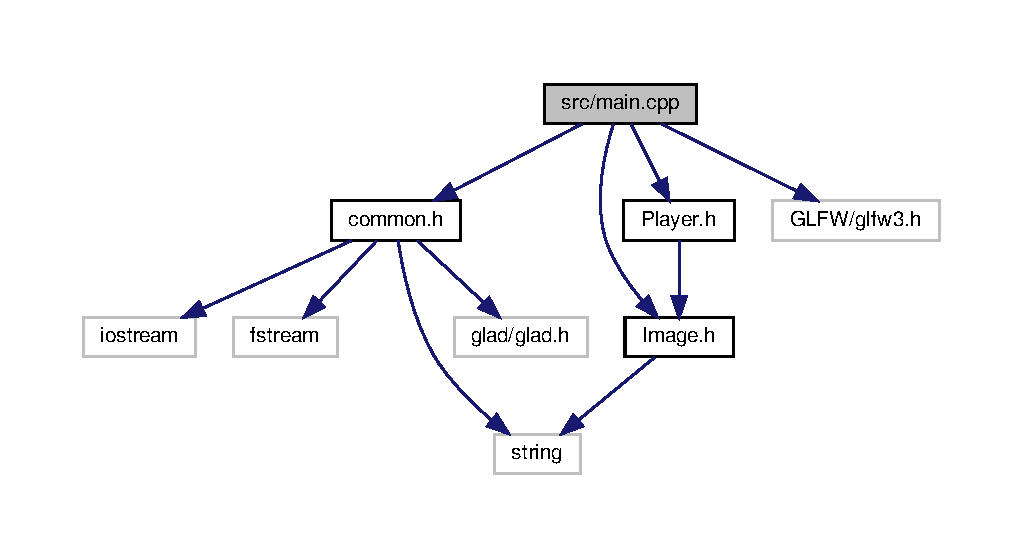
\includegraphics[width=350pt]{main_8cpp__incl}
\end{center}
\end{figure}
\subsection*{Classes}
\begin{DoxyCompactItemize}
\item 
struct \hyperlink{structInputState}{Input\+State}
\end{DoxyCompactItemize}
\subsection*{Macros}
\begin{DoxyCompactItemize}
\item 
\#define \hyperlink{main_8cpp_acaaeb59c827bcce5feadee7db40525b0}{G\+L\+F\+W\+\_\+\+D\+LL}
\end{DoxyCompactItemize}
\subsection*{Functions}
\begin{DoxyCompactItemize}
\item 
void \hyperlink{main_8cpp_aaa4abcb7f4846f711d52ad1b601a5d78}{On\+Keyboard\+Pressed} (G\+L\+F\+Wwindow $\ast$window, int key, int scancode, int action, int mode)
\item 
void \hyperlink{main_8cpp_aeffc3e0d1a1c5969bc1f3d177d78ae90}{process\+Player\+Movement} (\hyperlink{structPlayer}{Player} \&player)
\item 
void \hyperlink{main_8cpp_a6d05fb67cad0ce9a942c185ad4980aee}{On\+Mouse\+Button\+Clicked} (G\+L\+F\+Wwindow $\ast$window, int button, int action, int mods)
\item 
void \hyperlink{main_8cpp_a9460a3d7c16ac378e8448ddfe3f6e31e}{On\+Mouse\+Move} (G\+L\+F\+Wwindow $\ast$window, double xpos, double ypos)
\item 
void \hyperlink{main_8cpp_af0722419fcccf4242e0cce6decfcc14b}{On\+Mouse\+Scroll} (G\+L\+F\+Wwindow $\ast$window, double xoffset, double yoffset)
\item 
int \hyperlink{main_8cpp_affd9792de82327852d79df77c1261657}{init\+GL} ()
\item 
int \hyperlink{main_8cpp_a3c04138a5bfe5d72780bb7e82a18e627}{main} (int argc, char $\ast$$\ast$argv)
\end{DoxyCompactItemize}
\subsection*{Variables}
\begin{DoxyCompactItemize}
\item 
constexpr G\+Lsizei \hyperlink{main_8cpp_a6f9dfdfc4bf437ef692c4509b1dab1de}{W\+I\+N\+D\+O\+W\+\_\+\+W\+I\+D\+TH} = 1024
\item 
constexpr G\+Lsizei \hyperlink{main_8cpp_a526c9c10cab0f50a073d6ad4f7848295}{W\+I\+N\+D\+O\+W\+\_\+\+H\+E\+I\+G\+HT} = 1024
\item 
struct \hyperlink{structInputState}{Input\+State} \hyperlink{main_8cpp_aae98fcc029b6c75981e2489ab4ed42e5}{Input}
\item 
G\+Lfloat \hyperlink{main_8cpp_adf7cb443fa70a647d5603ee33b392102}{delta\+Time} = 0.\+0f
\item 
G\+Lfloat \hyperlink{main_8cpp_a606e9490a5462c2c60b30dc76ff573a1}{last\+Frame} = 0.\+0f
\end{DoxyCompactItemize}


\subsection{Macro Definition Documentation}
\mbox{\Hypertarget{main_8cpp_acaaeb59c827bcce5feadee7db40525b0}\label{main_8cpp_acaaeb59c827bcce5feadee7db40525b0}} 
\index{main.\+cpp@{main.\+cpp}!G\+L\+F\+W\+\_\+\+D\+LL@{G\+L\+F\+W\+\_\+\+D\+LL}}
\index{G\+L\+F\+W\+\_\+\+D\+LL@{G\+L\+F\+W\+\_\+\+D\+LL}!main.\+cpp@{main.\+cpp}}
\subsubsection{\texorpdfstring{G\+L\+F\+W\+\_\+\+D\+LL}{GLFW\_DLL}}
{\footnotesize\ttfamily \#define G\+L\+F\+W\+\_\+\+D\+LL}



\subsection{Function Documentation}
\mbox{\Hypertarget{main_8cpp_affd9792de82327852d79df77c1261657}\label{main_8cpp_affd9792de82327852d79df77c1261657}} 
\index{main.\+cpp@{main.\+cpp}!init\+GL@{init\+GL}}
\index{init\+GL@{init\+GL}!main.\+cpp@{main.\+cpp}}
\subsubsection{\texorpdfstring{init\+G\+L()}{initGL()}}
{\footnotesize\ttfamily int init\+GL (\begin{DoxyParamCaption}{ }\end{DoxyParamCaption})}

Here is the call graph for this function\+:
\nopagebreak
\begin{figure}[H]
\begin{center}
\leavevmode
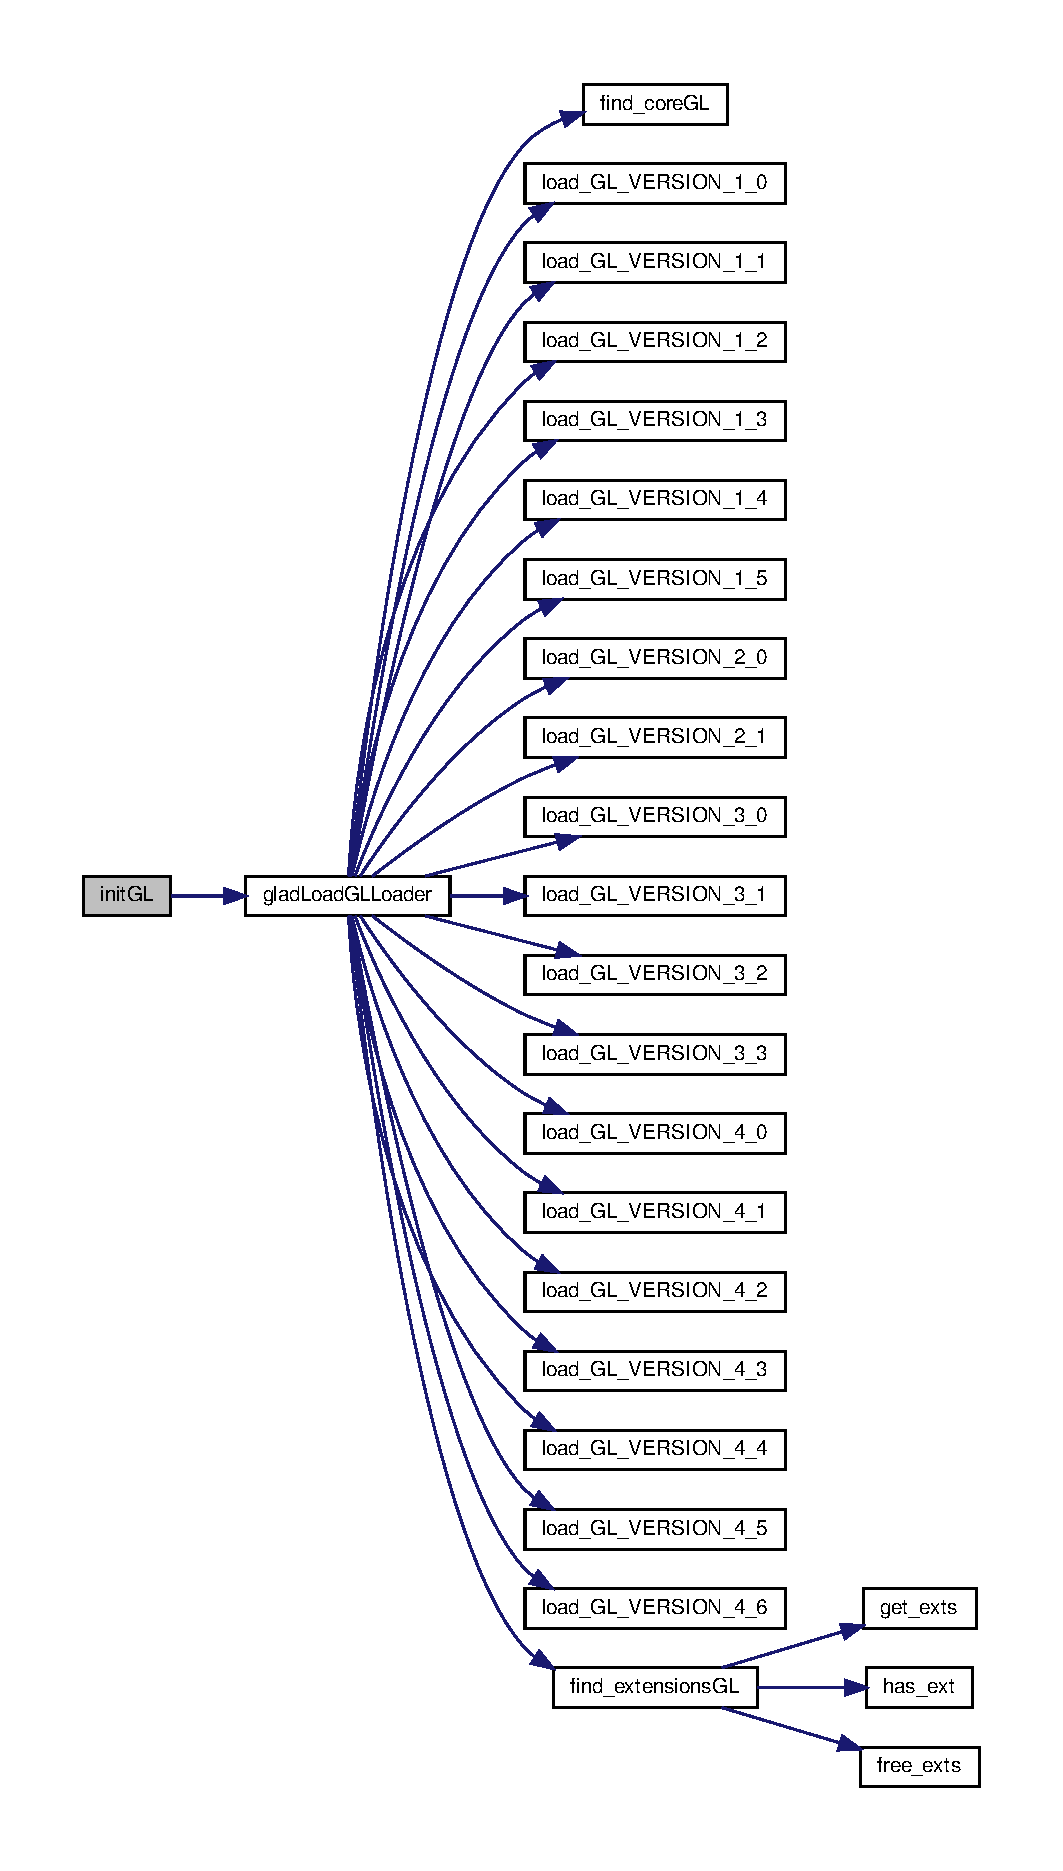
\includegraphics[height=550pt]{main_8cpp_affd9792de82327852d79df77c1261657_cgraph}
\end{center}
\end{figure}
Here is the caller graph for this function\+:
\nopagebreak
\begin{figure}[H]
\begin{center}
\leavevmode
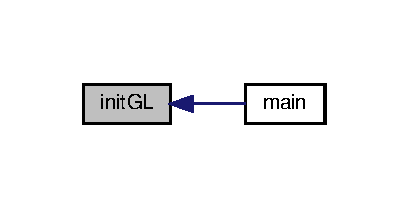
\includegraphics[width=196pt]{main_8cpp_affd9792de82327852d79df77c1261657_icgraph}
\end{center}
\end{figure}
\mbox{\Hypertarget{main_8cpp_a3c04138a5bfe5d72780bb7e82a18e627}\label{main_8cpp_a3c04138a5bfe5d72780bb7e82a18e627}} 
\index{main.\+cpp@{main.\+cpp}!main@{main}}
\index{main@{main}!main.\+cpp@{main.\+cpp}}
\subsubsection{\texorpdfstring{main()}{main()}}
{\footnotesize\ttfamily int main (\begin{DoxyParamCaption}\item[{int}]{argc,  }\item[{char $\ast$$\ast$}]{argv }\end{DoxyParamCaption})}

Here is the call graph for this function\+:
\nopagebreak
\begin{figure}[H]
\begin{center}
\leavevmode
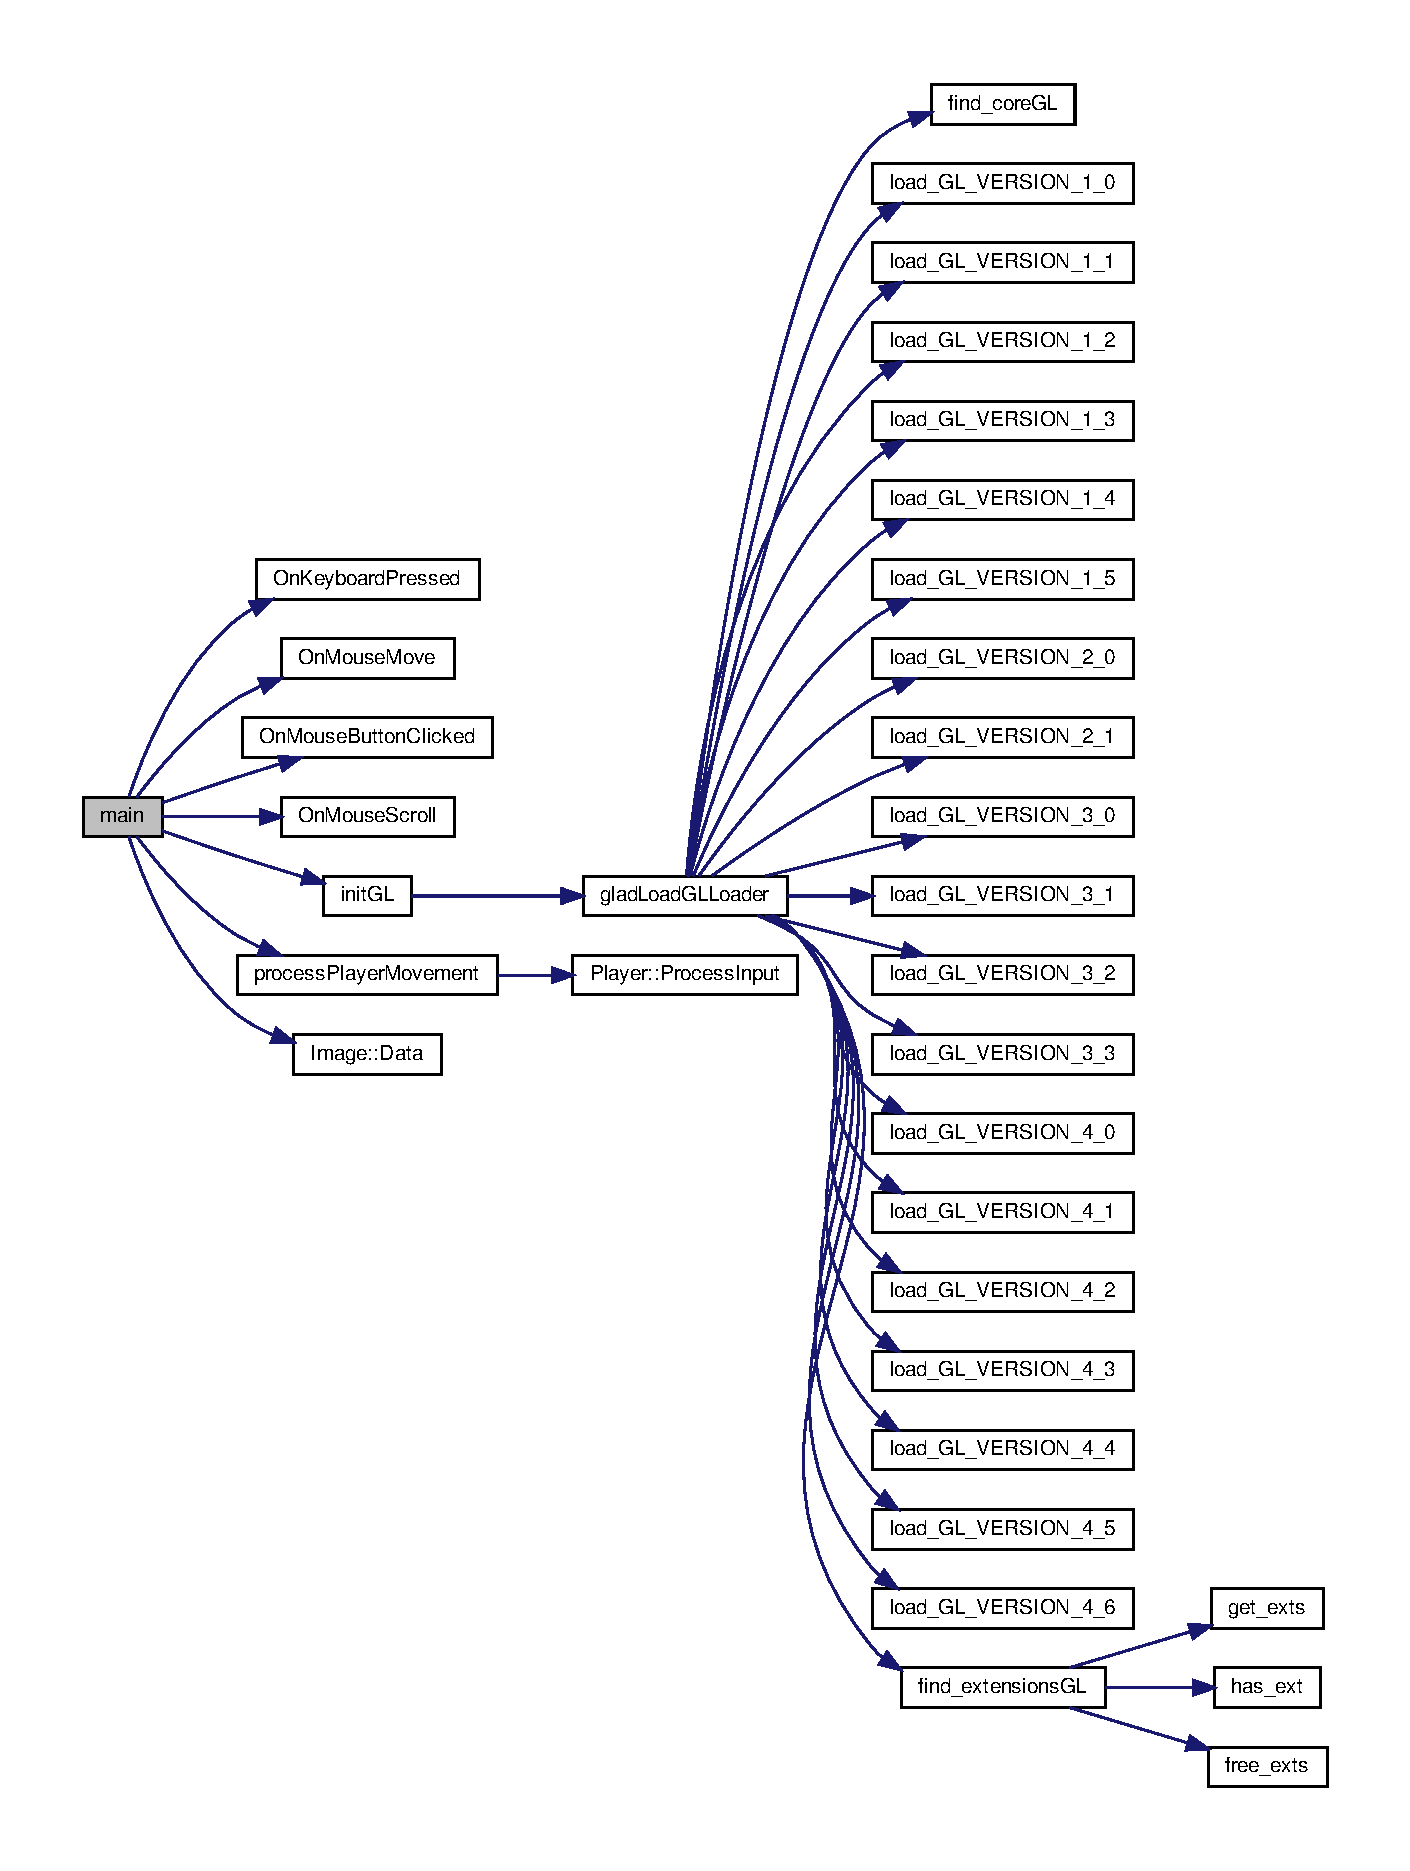
\includegraphics[width=350pt]{main_8cpp_a3c04138a5bfe5d72780bb7e82a18e627_cgraph}
\end{center}
\end{figure}
\mbox{\Hypertarget{main_8cpp_aaa4abcb7f4846f711d52ad1b601a5d78}\label{main_8cpp_aaa4abcb7f4846f711d52ad1b601a5d78}} 
\index{main.\+cpp@{main.\+cpp}!On\+Keyboard\+Pressed@{On\+Keyboard\+Pressed}}
\index{On\+Keyboard\+Pressed@{On\+Keyboard\+Pressed}!main.\+cpp@{main.\+cpp}}
\subsubsection{\texorpdfstring{On\+Keyboard\+Pressed()}{OnKeyboardPressed()}}
{\footnotesize\ttfamily void On\+Keyboard\+Pressed (\begin{DoxyParamCaption}\item[{G\+L\+F\+Wwindow $\ast$}]{window,  }\item[{int}]{key,  }\item[{int}]{scancode,  }\item[{int}]{action,  }\item[{int}]{mode }\end{DoxyParamCaption})}

Here is the caller graph for this function\+:
\nopagebreak
\begin{figure}[H]
\begin{center}
\leavevmode
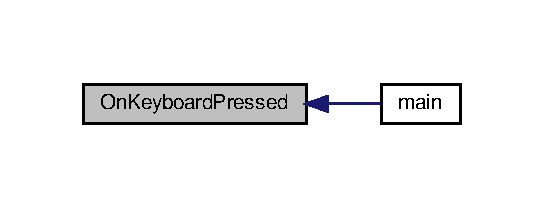
\includegraphics[width=261pt]{main_8cpp_aaa4abcb7f4846f711d52ad1b601a5d78_icgraph}
\end{center}
\end{figure}
\mbox{\Hypertarget{main_8cpp_a6d05fb67cad0ce9a942c185ad4980aee}\label{main_8cpp_a6d05fb67cad0ce9a942c185ad4980aee}} 
\index{main.\+cpp@{main.\+cpp}!On\+Mouse\+Button\+Clicked@{On\+Mouse\+Button\+Clicked}}
\index{On\+Mouse\+Button\+Clicked@{On\+Mouse\+Button\+Clicked}!main.\+cpp@{main.\+cpp}}
\subsubsection{\texorpdfstring{On\+Mouse\+Button\+Clicked()}{OnMouseButtonClicked()}}
{\footnotesize\ttfamily void On\+Mouse\+Button\+Clicked (\begin{DoxyParamCaption}\item[{G\+L\+F\+Wwindow $\ast$}]{window,  }\item[{int}]{button,  }\item[{int}]{action,  }\item[{int}]{mods }\end{DoxyParamCaption})}

Here is the caller graph for this function\+:
\nopagebreak
\begin{figure}[H]
\begin{center}
\leavevmode
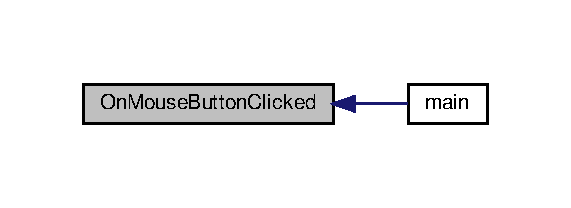
\includegraphics[width=274pt]{main_8cpp_a6d05fb67cad0ce9a942c185ad4980aee_icgraph}
\end{center}
\end{figure}
\mbox{\Hypertarget{main_8cpp_a9460a3d7c16ac378e8448ddfe3f6e31e}\label{main_8cpp_a9460a3d7c16ac378e8448ddfe3f6e31e}} 
\index{main.\+cpp@{main.\+cpp}!On\+Mouse\+Move@{On\+Mouse\+Move}}
\index{On\+Mouse\+Move@{On\+Mouse\+Move}!main.\+cpp@{main.\+cpp}}
\subsubsection{\texorpdfstring{On\+Mouse\+Move()}{OnMouseMove()}}
{\footnotesize\ttfamily void On\+Mouse\+Move (\begin{DoxyParamCaption}\item[{G\+L\+F\+Wwindow $\ast$}]{window,  }\item[{double}]{xpos,  }\item[{double}]{ypos }\end{DoxyParamCaption})}

Here is the caller graph for this function\+:
\nopagebreak
\begin{figure}[H]
\begin{center}
\leavevmode
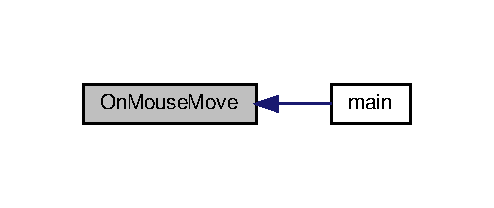
\includegraphics[width=237pt]{main_8cpp_a9460a3d7c16ac378e8448ddfe3f6e31e_icgraph}
\end{center}
\end{figure}
\mbox{\Hypertarget{main_8cpp_af0722419fcccf4242e0cce6decfcc14b}\label{main_8cpp_af0722419fcccf4242e0cce6decfcc14b}} 
\index{main.\+cpp@{main.\+cpp}!On\+Mouse\+Scroll@{On\+Mouse\+Scroll}}
\index{On\+Mouse\+Scroll@{On\+Mouse\+Scroll}!main.\+cpp@{main.\+cpp}}
\subsubsection{\texorpdfstring{On\+Mouse\+Scroll()}{OnMouseScroll()}}
{\footnotesize\ttfamily void On\+Mouse\+Scroll (\begin{DoxyParamCaption}\item[{G\+L\+F\+Wwindow $\ast$}]{window,  }\item[{double}]{xoffset,  }\item[{double}]{yoffset }\end{DoxyParamCaption})}

Here is the caller graph for this function\+:
\nopagebreak
\begin{figure}[H]
\begin{center}
\leavevmode
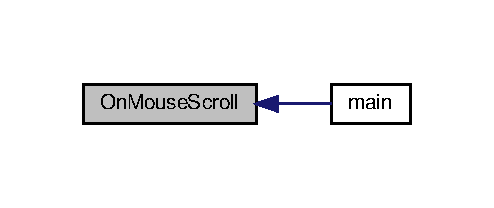
\includegraphics[width=237pt]{main_8cpp_af0722419fcccf4242e0cce6decfcc14b_icgraph}
\end{center}
\end{figure}
\mbox{\Hypertarget{main_8cpp_aeffc3e0d1a1c5969bc1f3d177d78ae90}\label{main_8cpp_aeffc3e0d1a1c5969bc1f3d177d78ae90}} 
\index{main.\+cpp@{main.\+cpp}!process\+Player\+Movement@{process\+Player\+Movement}}
\index{process\+Player\+Movement@{process\+Player\+Movement}!main.\+cpp@{main.\+cpp}}
\subsubsection{\texorpdfstring{process\+Player\+Movement()}{processPlayerMovement()}}
{\footnotesize\ttfamily void process\+Player\+Movement (\begin{DoxyParamCaption}\item[{\hyperlink{structPlayer}{Player} \&}]{player }\end{DoxyParamCaption})}

Here is the call graph for this function\+:
\nopagebreak
\begin{figure}[H]
\begin{center}
\leavevmode
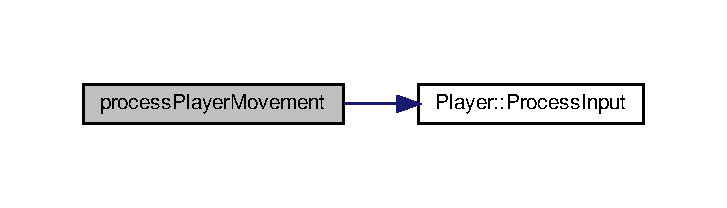
\includegraphics[width=349pt]{main_8cpp_aeffc3e0d1a1c5969bc1f3d177d78ae90_cgraph}
\end{center}
\end{figure}
Here is the caller graph for this function\+:
\nopagebreak
\begin{figure}[H]
\begin{center}
\leavevmode
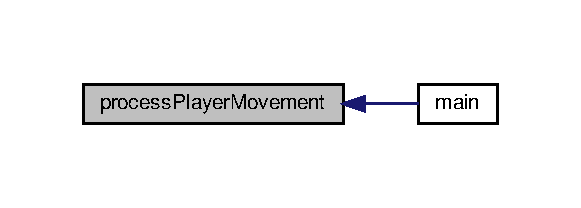
\includegraphics[width=279pt]{main_8cpp_aeffc3e0d1a1c5969bc1f3d177d78ae90_icgraph}
\end{center}
\end{figure}


\subsection{Variable Documentation}
\mbox{\Hypertarget{main_8cpp_adf7cb443fa70a647d5603ee33b392102}\label{main_8cpp_adf7cb443fa70a647d5603ee33b392102}} 
\index{main.\+cpp@{main.\+cpp}!delta\+Time@{delta\+Time}}
\index{delta\+Time@{delta\+Time}!main.\+cpp@{main.\+cpp}}
\subsubsection{\texorpdfstring{delta\+Time}{deltaTime}}
{\footnotesize\ttfamily G\+Lfloat delta\+Time = 0.\+0f}

\mbox{\Hypertarget{main_8cpp_aae98fcc029b6c75981e2489ab4ed42e5}\label{main_8cpp_aae98fcc029b6c75981e2489ab4ed42e5}} 
\index{main.\+cpp@{main.\+cpp}!Input@{Input}}
\index{Input@{Input}!main.\+cpp@{main.\+cpp}}
\subsubsection{\texorpdfstring{Input}{Input}}
{\footnotesize\ttfamily struct \hyperlink{structInputState}{Input\+State} Input}

\mbox{\Hypertarget{main_8cpp_a606e9490a5462c2c60b30dc76ff573a1}\label{main_8cpp_a606e9490a5462c2c60b30dc76ff573a1}} 
\index{main.\+cpp@{main.\+cpp}!last\+Frame@{last\+Frame}}
\index{last\+Frame@{last\+Frame}!main.\+cpp@{main.\+cpp}}
\subsubsection{\texorpdfstring{last\+Frame}{lastFrame}}
{\footnotesize\ttfamily G\+Lfloat last\+Frame = 0.\+0f}

\mbox{\Hypertarget{main_8cpp_a526c9c10cab0f50a073d6ad4f7848295}\label{main_8cpp_a526c9c10cab0f50a073d6ad4f7848295}} 
\index{main.\+cpp@{main.\+cpp}!W\+I\+N\+D\+O\+W\+\_\+\+H\+E\+I\+G\+HT@{W\+I\+N\+D\+O\+W\+\_\+\+H\+E\+I\+G\+HT}}
\index{W\+I\+N\+D\+O\+W\+\_\+\+H\+E\+I\+G\+HT@{W\+I\+N\+D\+O\+W\+\_\+\+H\+E\+I\+G\+HT}!main.\+cpp@{main.\+cpp}}
\subsubsection{\texorpdfstring{W\+I\+N\+D\+O\+W\+\_\+\+H\+E\+I\+G\+HT}{WINDOW\_HEIGHT}}
{\footnotesize\ttfamily constexpr G\+Lsizei W\+I\+N\+D\+O\+W\+\_\+\+H\+E\+I\+G\+HT = 1024}

\mbox{\Hypertarget{main_8cpp_a6f9dfdfc4bf437ef692c4509b1dab1de}\label{main_8cpp_a6f9dfdfc4bf437ef692c4509b1dab1de}} 
\index{main.\+cpp@{main.\+cpp}!W\+I\+N\+D\+O\+W\+\_\+\+W\+I\+D\+TH@{W\+I\+N\+D\+O\+W\+\_\+\+W\+I\+D\+TH}}
\index{W\+I\+N\+D\+O\+W\+\_\+\+W\+I\+D\+TH@{W\+I\+N\+D\+O\+W\+\_\+\+W\+I\+D\+TH}!main.\+cpp@{main.\+cpp}}
\subsubsection{\texorpdfstring{W\+I\+N\+D\+O\+W\+\_\+\+W\+I\+D\+TH}{WINDOW\_WIDTH}}
{\footnotesize\ttfamily constexpr G\+Lsizei W\+I\+N\+D\+O\+W\+\_\+\+W\+I\+D\+TH = 1024}


\hypertarget{Player_8cpp}{}\section{src/\+Player.cpp File Reference}
\label{Player_8cpp}\index{src/\+Player.\+cpp@{src/\+Player.\+cpp}}
{\ttfamily \#include \char`\"{}Player.\+h\char`\"{}}\newline
Include dependency graph for Player.\+cpp\+:\nopagebreak
\begin{figure}[H]
\begin{center}
\leavevmode
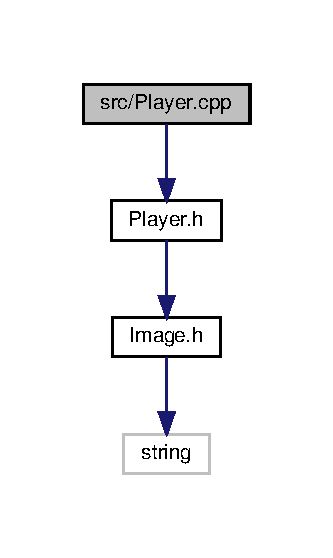
\includegraphics[width=160pt]{Player_8cpp__incl}
\end{center}
\end{figure}

%--- End generated contents ---

% Index
\backmatter
\newpage
\phantomsection
\clearemptydoublepage
\addcontentsline{toc}{chapter}{Index}
\printindex

\end{document}
